\documentclass[twoside]{book}

% Packages required by doxygen
\usepackage{fixltx2e}
\usepackage{calc}
\usepackage{doxygen}
\usepackage[export]{adjustbox} % also loads graphicx
\usepackage{graphicx}
\usepackage[utf8]{inputenc}
\usepackage{makeidx}
\usepackage{multicol}
\usepackage{multirow}
\PassOptionsToPackage{warn}{textcomp}
\usepackage{textcomp}
\usepackage[nointegrals]{wasysym}
\usepackage[table]{xcolor}

% Font selection
\usepackage[T1]{fontenc}
\usepackage[scaled=.90]{helvet}
\usepackage{courier}
\usepackage{amssymb}
\usepackage{sectsty}
\renewcommand{\familydefault}{\sfdefault}
\allsectionsfont{%
  \fontseries{bc}\selectfont%
  \color{darkgray}%
}
\renewcommand{\DoxyLabelFont}{%
  \fontseries{bc}\selectfont%
  \color{darkgray}%
}
\newcommand{\+}{\discretionary{\mbox{\scriptsize$\hookleftarrow$}}{}{}}

% Page & text layout
\usepackage{geometry}
\geometry{%
  a4paper,%
  top=2.5cm,%
  bottom=2.5cm,%
  left=2.5cm,%
  right=2.5cm%
}
\tolerance=750
\hfuzz=15pt
\hbadness=750
\setlength{\emergencystretch}{15pt}
\setlength{\parindent}{0cm}
\setlength{\parskip}{0.2cm}
\makeatletter
\renewcommand{\paragraph}{%
  \@startsection{paragraph}{4}{0ex}{-1.0ex}{1.0ex}{%
    \normalfont\normalsize\bfseries\SS@parafont%
  }%
}
\renewcommand{\subparagraph}{%
  \@startsection{subparagraph}{5}{0ex}{-1.0ex}{1.0ex}{%
    \normalfont\normalsize\bfseries\SS@subparafont%
  }%
}
\makeatother

% Headers & footers
\usepackage{fancyhdr}
\pagestyle{fancyplain}
\fancyhead[LE]{\fancyplain{}{\bfseries\thepage}}
\fancyhead[CE]{\fancyplain{}{}}
\fancyhead[RE]{\fancyplain{}{\bfseries\leftmark}}
\fancyhead[LO]{\fancyplain{}{\bfseries\rightmark}}
\fancyhead[CO]{\fancyplain{}{}}
\fancyhead[RO]{\fancyplain{}{\bfseries\thepage}}
\fancyfoot[LE]{\fancyplain{}{}}
\fancyfoot[CE]{\fancyplain{}{}}
\fancyfoot[RE]{\fancyplain{}{\bfseries\scriptsize Generated on Mon Feb 15 2016 15\+:47\+:55 for Bio\+Signal\+Pi by Doxygen }}
\fancyfoot[LO]{\fancyplain{}{\bfseries\scriptsize Generated on Mon Feb 15 2016 15\+:47\+:55 for Bio\+Signal\+Pi by Doxygen }}
\fancyfoot[CO]{\fancyplain{}{}}
\fancyfoot[RO]{\fancyplain{}{}}
\renewcommand{\footrulewidth}{0.4pt}
\renewcommand{\chaptermark}[1]{%
  \markboth{#1}{}%
}
\renewcommand{\sectionmark}[1]{%
  \markright{\thesection\ #1}%
}

% Indices & bibliography
\usepackage{natbib}
\usepackage[titles]{tocloft}
\setcounter{tocdepth}{3}
\setcounter{secnumdepth}{5}
\makeindex

% Hyperlinks (required, but should be loaded last)
\usepackage{ifpdf}
\ifpdf
  \usepackage[pdftex,pagebackref=true]{hyperref}
\else
  \usepackage[ps2pdf,pagebackref=true]{hyperref}
\fi
\hypersetup{%
  colorlinks=true,%
  linkcolor=blue,%
  citecolor=blue,%
  unicode%
}

% Custom commands
\newcommand{\clearemptydoublepage}{%
  \newpage{\pagestyle{empty}\cleardoublepage}%
}

\usepackage{caption}
\captionsetup{labelsep=space,justification=centering,font={bf},singlelinecheck=off,skip=4pt,position=top}

%===== C O N T E N T S =====

\begin{document}

% Titlepage & ToC
\hypersetup{pageanchor=false,
             bookmarks=true,
             bookmarksnumbered=true,
             pdfencoding=unicode
            }
\pagenumbering{roman}
\begin{titlepage}
\vspace*{7cm}
\begin{center}%
{\Large Bio\+Signal\+Pi \\[1ex]\large v2 }\\
\vspace*{1cm}
{\large Generated by Doxygen 1.8.11}\\
\vspace*{0.5cm}
{\small Mon Feb 15 2016 15:47:55}\\
\end{center}
\end{titlepage}
\clearemptydoublepage
\tableofcontents
\clearemptydoublepage
\pagenumbering{arabic}
\hypersetup{pageanchor=true}

%--- Begin generated contents ---
\chapter{Biosignal PI}
\label{index}\hypertarget{index}{}Biosignal PI aim is to provide a flexible and affordable open-\/source platform and tools for physiological and biological measurements such as blood pressure, blood glucose, weight, body composition, activity monitoring, and brain and cardiac activity.\+In first step, electrocardiogram (E\+CG) with wide usage in diagnosing and monitoring of heart disease and even in monitoring the autonomic nervous system through heart-\/rate variability (H\+RV) is developed.

This version provides 5-\/12 leads E\+CG and respiration measurement system based on Raspberry PI, a credit-\/card-\/size single-\/board computer, and A\+D\+A\+S1000. A\+D\+A\+S1000 is introduced by Analog Devices includes all the components necessary to perform a five-\/lead E\+CG digital conversion with respiration and pacemaker-\/artefact detection in a single chip. 



\subsubsection*{Functional Requirements\+:}


\begin{DoxyItemize}
\item Capture physiologicalsignal/data
\item Store captured data
\item Visualize sampled data in real time
\item Visualize sampled data from file
\item Process data
\end{DoxyItemize}

\subsubsection*{General Requirements\+:}


\begin{DoxyItemize}
\item Highly modular with interchangable parts
\item Extendable
\item Hardware independence
\item Easy to deploy
\item Testable classes,dependency reduction
\item Open-\/source 
\end{DoxyItemize}
\chapter{Todo List}
\label{todo}
\hypertarget{todo}{}

\begin{DoxyRefList}
\item[\label{todo__todo000021}%
\hypertarget{todo__todo000021}{}%
Member \hyperlink{classBluetoothMenu_a0fd16ad5a39ce3624613ad7834a55565}{Bluetooth\+Menu\+:\+:new\+Menu} ()]implement when Bluetooth functionallity is working for the R\+PI 

Implement to get Bluyetooth functionallity  
\item[\label{todo__todo000003}%
\hypertarget{todo__todo000003}{}%
Class \hyperlink{classConvertEcgToIbi}{Convert\+Ecg\+To\+Ibi} ]take different sort of files as input 
\item[\label{todo__todo000001}%
\hypertarget{todo__todo000001}{}%
Member \hyperlink{classConvertEcgToIbi_a3d9ea57ed19352295382095febc82f71}{Convert\+Ecg\+To\+Ibi\+:\+:run} ()]normalize input to work with more files 

F\+IX this check neater  
\item[\label{todo__todo000009}%
\hypertarget{todo__todo000009}{}%
Member \hyperlink{classDeviceManager_a8569742b2eb08d95052506e372b6bd31}{Device\+Manager\+:\+:stop} ()]use connected() before execution  
\item[\label{todo__todo000011}%
\hypertarget{todo__todo000011}{}%
Class \hyperlink{classEcgCapture}{Ecg\+Capture} ]Move all function descriptions from the .cpp file to the headerfile (.h file) \begin{DoxyAuthor}{Author}
Jonathan 

Martin  
\end{DoxyAuthor}

\item[\label{todo__todo000012}%
\hypertarget{todo__todo000012}{}%
Member \hyperlink{group__Device-Facade_ga8fef74cdd0296256ab4a700dae2d02a4}{Ecg\+Capture\+:\+:stop} ()]Implement 
\item[\label{todo__todo000013}%
\hypertarget{todo__todo000013}{}%
Module \hyperlink{group__HRV-Analysis}{H\+R\+V-\/\+Analysis} ]Add a function/class that takes a \hyperlink{classDataStream}{Data\+Stream} object as input and performs all the steps of the H\+RV Analysis taking E\+C\+G-\/\+Data as input and returning calculated H\+R\+V-\/\+Data.  
\item[\label{todo__todo000014}%
\hypertarget{todo__todo000014}{}%
File \hyperlink{hrvanalysis_8h}{hrvanalysis.h} ]add the ability to use a \hyperlink{classDataStream}{Data\+Stream} object as input for the H\+R\+V-\/functions.  
\item[\label{todo__todo000017}%
\hypertarget{todo__todo000017}{}%
Class \hyperlink{classHrvWidget}{Hrv\+Widget} ]Might be neccessary to set a upper limit for how large files to analyze. The qrs detection is the most computional demanding function called by \hyperlink{classHrvWidget}{Hrv\+Widget} 

Add a seperate Header\+Text\+Area to display information from Header textfile if that exists. 

Add the ability to use it for different sampling frequency sampling frequency is set in compile-\/time. Value set in Q\+R\+S\+D\+E\+T.\+h and \hyperlink{convertecgtoibi_8h}{convertecgtoibi.\+h}  
\item[\label{todo__todo000018}%
\hypertarget{todo__todo000018}{}%
Class \hyperlink{classLoadBigFile}{Load\+Big\+File} ]Could be integrated into \hyperlink{classDataLogger}{Data\+Logger} instead  
\item[\label{todo__todo000019}%
\hypertarget{todo__todo000019}{}%
Class \hyperlink{classMainWindow}{Main\+Window} ]add new Icons for the H\+R\+V-\/\+Widget and the Bluetooth\+Transfer-\/\+Widget 
\item[\label{todo__todo000016}%
\hypertarget{todo__todo000016}{}%
global\+Scope$>$ Member \hyperlink{group__HRV-Analysis_ga3cfec29967efe1561722a05d03f26158}{perform\+Freq\+Domain\+Hrv} (const Q\+Vector$<$ double $>$ $\ast$ibi\+Data, const Q\+Vector$<$ double $>$ $\ast$time\+Data, struct\+Freq\+\_\+T $\ast$output)]Add Ectopic Intervall Detection and Ectopic Interval Correction for the ibi\+Data 

Add Detrend for the ibi\+Data 
\item[\label{todo__todo000015}%
\hypertarget{todo__todo000015}{}%
global\+Scope$>$ Member \hyperlink{group__HRV-Analysis_ga2bd6c358a622e01babb7fdbca313c50f}{perform\+Time\+Domain\+Hrv} (const Q\+Vector$<$ double $>$ $\ast$ibi\+Data, struct0\+\_\+T $\ast$output)]Add Ectopic Intervall Detection and Ectopic Interval Correction for the ibi\+Data 
\item[\label{todo__todo000023}%
\hypertarget{todo__todo000023}{}%
Class \hyperlink{classPlotAndCaptureWidget}{Plot\+And\+Capture\+Widget} ]Move comments from .cpp file to header file (.h)  
\item[\label{todo__todo000024}%
\hypertarget{todo__todo000024}{}%
Member \hyperlink{classPlotAndCaptureWidget_a77ecf5a130215ce0246b8817e44081f7}{Plot\+And\+Capture\+Widget\+:\+:take\+Screen} ()]prevent overwriting previous snapshots  
\item[\label{todo__todo000025}%
\hypertarget{todo__todo000025}{}%
Class \hyperlink{classPlottingWidget}{Plotting\+Widget} ]Use the \hyperlink{classDataLogger}{Data\+Logger} instead of load\+Big\+File for reading data from txt and edf file. This needs to be implemented both in this class and also in the \hyperlink{classDataLogger}{Data\+Logger} Class. 
\item[\label{todo__todo000030}%
\hypertarget{todo__todo000030}{}%
Member \hyperlink{classSamplingThread_aade561b442e580b0ca4af112de2d7a41}{Sampling\+Thread\+:\+:close} ()]Implement function 

Implement  
\item[\label{todo__todo000029}%
\hypertarget{todo__todo000029}{}%
Member \hyperlink{classSamplingThread_a0770f5d1d0c0160cf023fae294010961}{Sampling\+Thread\+:\+:connected} ()]Implement function 

Implement \begin{DoxyReturn}{Returns}

\end{DoxyReturn}

\item[\label{todo__todo000028}%
\hypertarget{todo__todo000028}{}%
Member \hyperlink{classSamplingThread_aa52f1e7171ae5cb8432e949635b02d25}{Sampling\+Thread\+:\+:get\+Data} (\hyperlink{classDataStream}{Data\+Stream} \&)]
\item[\label{todo__todo000022}%
\hypertarget{todo__todo000022}{}%
Member \hyperlink{classSettingsMenu_abc441c12e8044c13f1a99791e2ee30d1}{Settings\+Menu\+:\+:new\+Menu} ()]Implement  
\item[\label{todo__todo000031}%
\hypertarget{todo__todo000031}{}%
Class \hyperlink{classSettingsSingleton}{Settings\+Singleton} ]Add verification functions controlling the input.  
\item[\label{todo__todo000033}%
\hypertarget{todo__todo000033}{}%
Class \hyperlink{classSettingsWidget}{Settings\+Widget} ]Add some sort of input-\/control for validating that the entered data is \char`\"{}correct\char`\"{} 
\end{DoxyRefList}
\chapter{Deprecated List}
\label{deprecated}
\hypertarget{deprecated}{}

\begin{DoxyRefList}
\item[\label{deprecated__deprecated000001}%
\hypertarget{deprecated__deprecated000001}{}%
Member \hyperlink{classDeviceManager_a322e3bd6b6f57692116b6af7b9a57a9a}{Device\+Manager\+:\+:collect\+Data} (\hyperlink{classDataStream}{Data\+Stream} \&)]
\item[\label{deprecated__deprecated000002}%
\hypertarget{deprecated__deprecated000002}{}%
Member \hyperlink{group__Device-Facade_ga9f04dad928d472c92229f3f39a8f2445}{Ecg\+Capture\+:\+:test\+Device} ()]Currently not in use.  
\item[\label{deprecated__deprecated000003}%
\hypertarget{deprecated__deprecated000003}{}%
Member \hyperlink{classEcgMock_aaa2628c0e8364980e6f252dfc3b86d1a}{Ecg\+Mock\+:\+:get\+Data} (\hyperlink{classDataStream}{Data\+Stream} \&)]old function, not used 
\begin{DoxyParams}{Parameters}
{\em \hyperlink{classDataStream}{Data\+Stream}} & \& \\
\hline
\end{DoxyParams}

\item[\label{deprecated__deprecated000007}%
\hypertarget{deprecated__deprecated000007}{}%
Member \hyperlink{classSamplingThread_aa52f1e7171ae5cb8432e949635b02d25}{Sampling\+Thread\+:\+:get\+Data} (\hyperlink{classDataStream}{Data\+Stream} \&)]Not used 
\end{DoxyRefList}
\chapter{Bug List}
\label{bug}
\hypertarget{bug}{}

\begin{DoxyRefList}
\item[\label{bug__bug000003}%
\hypertarget{bug__bug000003}{}%
Class \hyperlink{classEcgCapture}{Ecg\+Capture} ]Crashes with a Q\+Vector index out of range. Problem caused by the read\+Frame function when it dosent provide a array with at least 5 elements  
\item[\label{bug__bug000006}%
\hypertarget{bug__bug000006}{}%
Member \hyperlink{classEcgCaptureMenu_a610d2985e09cd56cb381e6e443dbbc72}{Ecg\+Capture\+Menu\+:\+:new\+Menu} ()]The program will freeze after the capturing is stopped since the stop function isn\textquotesingle{}t implemented with a return statement  
\item[\label{bug__bug000004}%
\hypertarget{bug__bug000004}{}%
Class \hyperlink{classEcgMock}{Ecg\+Mock} ]No known Bugs  
\item[\label{bug__bug000005}%
\hypertarget{bug__bug000005}{}%
Class \hyperlink{classHrvWidget}{Hrv\+Widget} ]Might crash or work incorrectly for \char`\"{}wrong\char`\"{} formated E\+C\+G-\/files
\end{DoxyRefList}
\chapter{Module Index}
\section{Modules}
Here is a list of all modules\+:\begin{DoxyCompactList}
\item \contentsline{section}{H\+R\+V-\/\+Analysis}{\pageref{group__HRV-Analysis}}{}
\item \contentsline{section}{Data\+Logger}{\pageref{group__DataLogger}}{}
\item \contentsline{section}{Device-\/\+Facade}{\pageref{group__Device-Facade}}{}
\end{DoxyCompactList}

\chapter{Namespace Index}
\section{Namespace List}
Here is a list of all namespaces with brief descriptions\+:\begin{DoxyCompactList}
\item\contentsline{section}{\hyperlink{namespaceUi}{Ui} }{\pageref{namespaceUi}}{}
\end{DoxyCompactList}

\chapter{Hierarchical Index}
\section{Class Hierarchy}
This inheritance list is sorted roughly, but not completely, alphabetically\+:\begin{DoxyCompactList}
\item \contentsline{section}{Abstract\+Menu}{\pageref{classAbstractMenu}}{}
\begin{DoxyCompactList}
\item \contentsline{section}{Base\+Menu}{\pageref{classBaseMenu}}{}
\begin{DoxyCompactList}
\item \contentsline{section}{Bluetooth\+Menu}{\pageref{classBluetoothMenu}}{}
\item \contentsline{section}{Ecg\+Capture\+Menu}{\pageref{classEcgCaptureMenu}}{}
\begin{DoxyCompactList}
\item \contentsline{section}{Settings\+Menu}{\pageref{classSettingsMenu}}{}
\end{DoxyCompactList}
\end{DoxyCompactList}
\end{DoxyCompactList}
\item \contentsline{section}{Ecg\+Stream\+Object}{\pageref{structEcgStreamObject}}{}
\item Q\+Dialog\begin{DoxyCompactList}
\item \contentsline{section}{pin\+Display}{\pageref{classpinDisplay}}{}
\item \contentsline{section}{Progress}{\pageref{classProgress}}{}
\item \contentsline{section}{Remote\+Selector}{\pageref{classRemoteSelector}}{}
\end{DoxyCompactList}
\item Q\+Object\begin{DoxyCompactList}
\item \contentsline{section}{Data\+Logger}{\pageref{classDataLogger}}{}
\item \contentsline{section}{Ecg\+Capture}{\pageref{classEcgCapture}}{}
\item \contentsline{section}{Pi\+Face\+Control\+And\+View}{\pageref{classPiFaceControlAndView}}{}
\end{DoxyCompactList}
\item Q\+Thread\begin{DoxyCompactList}
\item \contentsline{section}{Convert\+Ecg\+To\+Ibi}{\pageref{classConvertEcgToIbi}}{}
\item \contentsline{section}{Device\+Interface}{\pageref{classDeviceInterface}}{}
\begin{DoxyCompactList}
\item \contentsline{section}{Ecg\+Mock}{\pageref{classEcgMock}}{}
\item \contentsline{section}{Sampling\+Thread}{\pageref{classSamplingThread}}{}
\end{DoxyCompactList}
\item \contentsline{section}{Device\+Manager}{\pageref{classDeviceManager}}{}
\item \contentsline{section}{Load\+Big\+File}{\pageref{classLoadBigFile}}{}
\end{DoxyCompactList}
\item Q\+Vector\begin{DoxyCompactList}
\item \contentsline{section}{Data\+Stream}{\pageref{classDataStream}}{}
\end{DoxyCompactList}
\item Q\+Widget\begin{DoxyCompactList}
\item \contentsline{section}{Home\+Page\+Widget}{\pageref{classHomePageWidget}}{}
\item \contentsline{section}{Hrv\+Widget}{\pageref{classHrvWidget}}{}
\item \contentsline{section}{Main\+Window}{\pageref{classMainWindow}}{}
\item \contentsline{section}{Plot\+And\+Capture\+Widget}{\pageref{classPlotAndCaptureWidget}}{}
\item \contentsline{section}{Plotting\+Widget}{\pageref{classPlottingWidget}}{}
\item \contentsline{section}{Settings\+Widget}{\pageref{classSettingsWidget}}{}
\item \contentsline{section}{Slider\+Widget}{\pageref{classSliderWidget}}{}
\end{DoxyCompactList}
\item Qwt\+Array\+Series\+Data\begin{DoxyCompactList}
\item \contentsline{section}{Curve\+Data}{\pageref{classCurveData}}{}
\end{DoxyCompactList}
\item Qwt\+Plot\begin{DoxyCompactList}
\item \contentsline{section}{Plot}{\pageref{classPlot}}{}
\end{DoxyCompactList}
\item \contentsline{section}{Settings\+Singleton}{\pageref{classSettingsSingleton}}{}
\end{DoxyCompactList}

\chapter{Class Index}
\section{Class List}
Here are the classes, structs, unions and interfaces with brief descriptions\+:\begin{DoxyCompactList}
\item\contentsline{section}{\hyperlink{classAbstractMenu}{Abstract\+Menu} \\*Abstract menu object for Pi\+Face C\+AD }{\pageref{classAbstractMenu}}{}
\item\contentsline{section}{\hyperlink{classBaseMenu}{Base\+Menu} \\*Homepage of the Menu-\/system for the Pi\+Face G\+UI }{\pageref{classBaseMenu}}{}
\item\contentsline{section}{\hyperlink{classBluetoothMenu}{Bluetooth\+Menu} \\*The \hyperlink{classBluetoothMenu}{Bluetooth\+Menu} class }{\pageref{classBluetoothMenu}}{}
\item\contentsline{section}{\hyperlink{classConvertEcgToIbi}{Convert\+Ecg\+To\+Ibi} \\*Converts textfile with E\+C\+G-\/data into I\+BI file }{\pageref{classConvertEcgToIbi}}{}
\item\contentsline{section}{\hyperlink{classCurveData}{Curve\+Data} }{\pageref{classCurveData}}{}
\item\contentsline{section}{\hyperlink{classDataLogger}{Data\+Logger} \\*The \hyperlink{classDataLogger}{Data\+Logger} class }{\pageref{classDataLogger}}{}
\item\contentsline{section}{\hyperlink{classDataStream}{Data\+Stream} \\*Abstract Interface that should be used for storing data in the memory }{\pageref{classDataStream}}{}
\item\contentsline{section}{\hyperlink{classDeviceInterface}{Device\+Interface} \\*Abstract interface for all devices }{\pageref{classDeviceInterface}}{}
\item\contentsline{section}{\hyperlink{classDeviceManager}{Device\+Manager} \\*Handles which device to connect through the \hyperlink{classDeviceInterface}{Device\+Interface} }{\pageref{classDeviceManager}}{}
\item\contentsline{section}{\hyperlink{classEcgCapture}{Ecg\+Capture} \\*Responsible for communication with A\+D\+AS }{\pageref{classEcgCapture}}{}
\item\contentsline{section}{\hyperlink{classEcgCaptureMenu}{Ecg\+Capture\+Menu} \\*Menu were the user can chosse between \hyperlink{classSettingsMenu}{Settings\+Menu} or starting E\+C\+G-\/capture The start menu starts the E\+C\+G-\/capture and will capture until pressed again }{\pageref{classEcgCaptureMenu}}{}
\item\contentsline{section}{\hyperlink{classEcgMock}{Ecg\+Mock} \\*Mock version of an device The \hyperlink{classEcgMock}{Ecg\+Mock} device will return sine and cosine functions as data }{\pageref{classEcgMock}}{}
\item\contentsline{section}{\hyperlink{structEcgStreamObject}{Ecg\+Stream\+Object} \\*Struct to store Biosignal data from a specific time, combined with \hyperlink{classDataStream}{Data\+Stream} it will store a sequence of sampled data }{\pageref{structEcgStreamObject}}{}
\item\contentsline{section}{\hyperlink{classHomePageWidget}{Home\+Page\+Widget} \\*Startpage for the Biosignal PI software }{\pageref{classHomePageWidget}}{}
\item\contentsline{section}{\hyperlink{classHrvWidget}{Hrv\+Widget} \\*Widget responsible for the graphical interface of the H\+RV Analysis }{\pageref{classHrvWidget}}{}
\item\contentsline{section}{\hyperlink{classLoadBigFile}{Load\+Big\+File} \\*Class used to load a big .txt file in a new thread }{\pageref{classLoadBigFile}}{}
\item\contentsline{section}{\hyperlink{classMainWindow}{Main\+Window} \\*\hyperlink{classMainWindow}{Main\+Window} holds all the different parts of the G\+UI Implements the different widgets used in the G\+UI and let the user decide wich widget to use by clicking the approbiate icon representing the different widgets the Biosignal PI software contains of }{\pageref{classMainWindow}}{}
\item\contentsline{section}{\hyperlink{classPiFaceControlAndView}{Pi\+Face\+Control\+And\+View} \\*Handles the eventloop of the Pi\+Face G\+UI }{\pageref{classPiFaceControlAndView}}{}
\item\contentsline{section}{\hyperlink{classpinDisplay}{pin\+Display} }{\pageref{classpinDisplay}}{}
\item\contentsline{section}{\hyperlink{classPlot}{Plot} \\*Extension of Qwt\+Plot used for plotting data }{\pageref{classPlot}}{}
\item\contentsline{section}{\hyperlink{classPlotAndCaptureWidget}{Plot\+And\+Capture\+Widget} \\*Widget used for capture and plotting of data from the connected \hyperlink{classDeviceManager}{Device\+Manager} }{\pageref{classPlotAndCaptureWidget}}{}
\item\contentsline{section}{\hyperlink{classPlottingWidget}{Plotting\+Widget} \\*Widget that can read E\+CG information from file and plots the data }{\pageref{classPlottingWidget}}{}
\item\contentsline{section}{\hyperlink{classProgress}{Progress} }{\pageref{classProgress}}{}
\item\contentsline{section}{\hyperlink{classRemoteSelector}{Remote\+Selector} }{\pageref{classRemoteSelector}}{}
\item\contentsline{section}{\hyperlink{classSamplingThread}{Sampling\+Thread} \\*\hyperlink{classDeviceInterface}{Device\+Interface} Class responsible for sampling E\+CG }{\pageref{classSamplingThread}}{}
\item\contentsline{section}{\hyperlink{classSettingsMenu}{Settings\+Menu} \\*For the Pi\+Face G\+UI }{\pageref{classSettingsMenu}}{}
\item\contentsline{section}{\hyperlink{classSettingsSingleton}{Settings\+Singleton} \\*Singleton containing all settings used by the Biosignal PI Framework }{\pageref{classSettingsSingleton}}{}
\item\contentsline{section}{\hyperlink{classSettingsWidget}{Settings\+Widget} \\*Widget used to change the different settings in \hyperlink{classSettingsWidget}{Settings\+Widget} }{\pageref{classSettingsWidget}}{}
\item\contentsline{section}{\hyperlink{classSliderWidget}{Slider\+Widget} \\*Class used by \hyperlink{classPlottingWidget}{Plotting\+Widget} to enable a slider for the different signals plotted }{\pageref{classSliderWidget}}{}
\end{DoxyCompactList}

\chapter{File Index}
\section{File List}
Here is a list of all files with brief descriptions\+:\begin{DoxyCompactList}
\item\contentsline{section}{src/\hyperlink{convertecgtoibi_8cpp}{convertecgtoibi.\+cpp} }{\pageref{convertecgtoibi_8cpp}}{}
\item\contentsline{section}{src/\hyperlink{convertecgtoibi_8h}{convertecgtoibi.\+h} }{\pageref{convertecgtoibi_8h}}{}
\item\contentsline{section}{src/\hyperlink{datalogger_8cpp}{datalogger.\+cpp} }{\pageref{datalogger_8cpp}}{}
\item\contentsline{section}{src/\hyperlink{datalogger_8h}{datalogger.\+h} }{\pageref{datalogger_8h}}{}
\item\contentsline{section}{src/\hyperlink{datastream_8cpp}{datastream.\+cpp} }{\pageref{datastream_8cpp}}{}
\item\contentsline{section}{src/\hyperlink{datastream_8h}{datastream.\+h} }{\pageref{datastream_8h}}{}
\item\contentsline{section}{src/\hyperlink{deviceinterface_8cpp}{deviceinterface.\+cpp} }{\pageref{deviceinterface_8cpp}}{}
\item\contentsline{section}{src/\hyperlink{deviceinterface_8h}{deviceinterface.\+h} }{\pageref{deviceinterface_8h}}{}
\item\contentsline{section}{src/\hyperlink{devicemanager_8cpp}{devicemanager.\+cpp} }{\pageref{devicemanager_8cpp}}{}
\item\contentsline{section}{src/\hyperlink{devicemanager_8h}{devicemanager.\+h} }{\pageref{devicemanager_8h}}{}
\item\contentsline{section}{src/\hyperlink{ecgcapture_8cpp}{ecgcapture.\+cpp} }{\pageref{ecgcapture_8cpp}}{}
\item\contentsline{section}{src/\hyperlink{ecgcapture_8h}{ecgcapture.\+h} }{\pageref{ecgcapture_8h}}{}
\item\contentsline{section}{src/\hyperlink{ecgmock_8cpp}{ecgmock.\+cpp} }{\pageref{ecgmock_8cpp}}{}
\item\contentsline{section}{src/\hyperlink{ecgmock_8h}{ecgmock.\+h} }{\pageref{ecgmock_8h}}{}
\item\contentsline{section}{src/\hyperlink{ecgstreamobject_8cpp}{ecgstreamobject.\+cpp} }{\pageref{ecgstreamobject_8cpp}}{}
\item\contentsline{section}{src/\hyperlink{ecgstreamobject_8h}{ecgstreamobject.\+h} }{\pageref{ecgstreamobject_8h}}{}
\item\contentsline{section}{src/\hyperlink{homepagewidget_8cpp}{homepagewidget.\+cpp} }{\pageref{homepagewidget_8cpp}}{}
\item\contentsline{section}{src/\hyperlink{homepagewidget_8h}{homepagewidget.\+h} }{\pageref{homepagewidget_8h}}{}
\item\contentsline{section}{src/\hyperlink{hrvanalysis_8cpp}{hrvanalysis.\+cpp} }{\pageref{hrvanalysis_8cpp}}{}
\item\contentsline{section}{src/\hyperlink{hrvanalysis_8h}{hrvanalysis.\+h} \\*Collection of functions used to interact with the Matlab Coder generated H\+R\+V-\/functions }{\pageref{hrvanalysis_8h}}{}
\item\contentsline{section}{src/\hyperlink{hrvwidget_8cpp}{hrvwidget.\+cpp} }{\pageref{hrvwidget_8cpp}}{}
\item\contentsline{section}{src/\hyperlink{hrvwidget_8h}{hrvwidget.\+h} }{\pageref{hrvwidget_8h}}{}
\item\contentsline{section}{src/\hyperlink{loadbigfile_8cpp}{loadbigfile.\+cpp} }{\pageref{loadbigfile_8cpp}}{}
\item\contentsline{section}{src/\hyperlink{loadbigfile_8h}{loadbigfile.\+h} }{\pageref{loadbigfile_8h}}{}
\item\contentsline{section}{src/\hyperlink{main_8cpp}{main.\+cpp} }{\pageref{main_8cpp}}{}
\item\contentsline{section}{src/\hyperlink{mainwindow_8cpp}{mainwindow.\+cpp} }{\pageref{mainwindow_8cpp}}{}
\item\contentsline{section}{src/\hyperlink{mainwindow_8h}{mainwindow.\+h} }{\pageref{mainwindow_8h}}{}
\item\contentsline{section}{src/\hyperlink{meanFilter_8cpp}{mean\+Filter.\+cpp} }{\pageref{meanFilter_8cpp}}{}
\item\contentsline{section}{src/\hyperlink{meanFilter_8h}{mean\+Filter.\+h} }{\pageref{meanFilter_8h}}{}
\item\contentsline{section}{src/\hyperlink{plot_8cpp}{plot.\+cpp} }{\pageref{plot_8cpp}}{}
\item\contentsline{section}{src/\hyperlink{plot_8h}{plot.\+h} }{\pageref{plot_8h}}{}
\item\contentsline{section}{src/\hyperlink{plotandcapturewidget_8cpp}{plotandcapturewidget.\+cpp} }{\pageref{plotandcapturewidget_8cpp}}{}
\item\contentsline{section}{src/\hyperlink{plotandcapturewidget_8h}{plotandcapturewidget.\+h} }{\pageref{plotandcapturewidget_8h}}{}
\item\contentsline{section}{src/\hyperlink{plottingwidget_8cpp}{plottingwidget.\+cpp} }{\pageref{plottingwidget_8cpp}}{}
\item\contentsline{section}{src/\hyperlink{plottingwidget_8h}{plottingwidget.\+h} }{\pageref{plottingwidget_8h}}{}
\item\contentsline{section}{src/\hyperlink{samplingthread_8cpp}{samplingthread.\+cpp} }{\pageref{samplingthread_8cpp}}{}
\item\contentsline{section}{src/\hyperlink{samplingthread_8h}{samplingthread.\+h} }{\pageref{samplingthread_8h}}{}
\item\contentsline{section}{src/\hyperlink{settingssingleton_8cpp}{settingssingleton.\+cpp} }{\pageref{settingssingleton_8cpp}}{}
\item\contentsline{section}{src/\hyperlink{settingssingleton_8h}{settingssingleton.\+h} }{\pageref{settingssingleton_8h}}{}
\item\contentsline{section}{src/\hyperlink{settingswidget_8cpp}{settingswidget.\+cpp} }{\pageref{settingswidget_8cpp}}{}
\item\contentsline{section}{src/\hyperlink{settingswidget_8h}{settingswidget.\+h} }{\pageref{settingswidget_8h}}{}
\item\contentsline{section}{src/\hyperlink{sliderwidget_8cpp}{sliderwidget.\+cpp} }{\pageref{sliderwidget_8cpp}}{}
\item\contentsline{section}{src/\hyperlink{sliderwidget_8h}{sliderwidget.\+h} }{\pageref{sliderwidget_8h}}{}
\item\contentsline{section}{src/\+Pi\+Face-\/\+Interface/\hyperlink{abstractmenu_8cpp}{abstractmenu.\+cpp} }{\pageref{abstractmenu_8cpp}}{}
\item\contentsline{section}{src/\+Pi\+Face-\/\+Interface/\hyperlink{abstractmenu_8h}{abstractmenu.\+h} }{\pageref{abstractmenu_8h}}{}
\item\contentsline{section}{src/\+Pi\+Face-\/\+Interface/\hyperlink{basemenu_8cpp}{basemenu.\+cpp} }{\pageref{basemenu_8cpp}}{}
\item\contentsline{section}{src/\+Pi\+Face-\/\+Interface/\hyperlink{basemenu_8h}{basemenu.\+h} }{\pageref{basemenu_8h}}{}
\item\contentsline{section}{src/\+Pi\+Face-\/\+Interface/\hyperlink{bluetoothmenu_8cpp}{bluetoothmenu.\+cpp} }{\pageref{bluetoothmenu_8cpp}}{}
\item\contentsline{section}{src/\+Pi\+Face-\/\+Interface/\hyperlink{bluetoothmenu_8h}{bluetoothmenu.\+h} }{\pageref{bluetoothmenu_8h}}{}
\item\contentsline{section}{src/\+Pi\+Face-\/\+Interface/\hyperlink{ecgcapturemenu_8cpp}{ecgcapturemenu.\+cpp} }{\pageref{ecgcapturemenu_8cpp}}{}
\item\contentsline{section}{src/\+Pi\+Face-\/\+Interface/\hyperlink{ecgcapturemenu_8h}{ecgcapturemenu.\+h} }{\pageref{ecgcapturemenu_8h}}{}
\item\contentsline{section}{src/\+Pi\+Face-\/\+Interface/\hyperlink{PiFace-Interface_2main_8cpp}{main.\+cpp} }{\pageref{PiFace-Interface_2main_8cpp}}{}
\item\contentsline{section}{src/\+Pi\+Face-\/\+Interface/\hyperlink{pifacecontrolandview_8cpp}{pifacecontrolandview.\+cpp} }{\pageref{pifacecontrolandview_8cpp}}{}
\item\contentsline{section}{src/\+Pi\+Face-\/\+Interface/\hyperlink{pifacecontrolandview_8h}{pifacecontrolandview.\+h} }{\pageref{pifacecontrolandview_8h}}{}
\item\contentsline{section}{src/\+Pi\+Face-\/\+Interface/\hyperlink{settingsmenu_8cpp}{settingsmenu.\+cpp} }{\pageref{settingsmenu_8cpp}}{}
\item\contentsline{section}{src/\+Pi\+Face-\/\+Interface/\hyperlink{settingsmenu_8h}{settingsmenu.\+h} }{\pageref{settingsmenu_8h}}{}
\item\contentsline{section}{src/\+Qt-\/btfiletransfer/\hyperlink{pindisplay_8cpp}{pindisplay.\+cpp} }{\pageref{pindisplay_8cpp}}{}
\item\contentsline{section}{src/\+Qt-\/btfiletransfer/\hyperlink{pindisplay_8h}{pindisplay.\+h} }{\pageref{pindisplay_8h}}{}
\item\contentsline{section}{src/\+Qt-\/btfiletransfer/\hyperlink{progress_8cpp}{progress.\+cpp} }{\pageref{progress_8cpp}}{}
\item\contentsline{section}{src/\+Qt-\/btfiletransfer/\hyperlink{progress_8h}{progress.\+h} }{\pageref{progress_8h}}{}
\item\contentsline{section}{src/\+Qt-\/btfiletransfer/\hyperlink{remoteselector_8cpp}{remoteselector.\+cpp} }{\pageref{remoteselector_8cpp}}{}
\item\contentsline{section}{src/\+Qt-\/btfiletransfer/\hyperlink{remoteselector_8h}{remoteselector.\+h} }{\pageref{remoteselector_8h}}{}
\end{DoxyCompactList}

\chapter{Module Documentation}
\hypertarget{group__HRV-Analysis}{}\section{H\+R\+V-\/\+Analysis}
\label{group__HRV-Analysis}\index{H\+R\+V-\/\+Analysis@{H\+R\+V-\/\+Analysis}}


Classes and Functions used for H\+R\+V-\/\+Analysis.  


\subsection*{Files}
\begin{DoxyCompactItemize}
\item 
file \hyperlink{hrvanalysis_8h}{hrvanalysis.\+h}
\begin{DoxyCompactList}\small\item\em Collection of functions used to interact with the Matlab Coder generated H\+R\+V-\/functions. \end{DoxyCompactList}\end{DoxyCompactItemize}
\subsection*{Classes}
\begin{DoxyCompactItemize}
\item 
class \hyperlink{classConvertEcgToIbi}{Convert\+Ecg\+To\+Ibi}
\begin{DoxyCompactList}\small\item\em Converts textfile with E\+C\+G-\/data into I\+BI file. \end{DoxyCompactList}\end{DoxyCompactItemize}
\subsection*{Functions}
\begin{DoxyCompactItemize}
\item 
int \hyperlink{group__HRV-Analysis_ga5c14f0d7dd58dec49e939470bcb5db1c}{Q\+R\+S\+Det} (int, int)
\begin{DoxyCompactList}\small\item\em Q\+R\+S\+Det Function used for the Q\+R\+S-\/detection. \end{DoxyCompactList}\item 
void \hyperlink{group__HRV-Analysis_ga2bd6c358a622e01babb7fdbca313c50f}{perform\+Time\+Domain\+Hrv} (const Q\+Vector$<$ double $>$ $\ast$ibi\+Data, struct0\+\_\+T $\ast$output)
\begin{DoxyCompactList}\small\item\em Performs the Statistical Time Domain calculations for H\+RV Analysis. \end{DoxyCompactList}\item 
void \hyperlink{group__HRV-Analysis_ga3cfec29967efe1561722a05d03f26158}{perform\+Freq\+Domain\+Hrv} (const Q\+Vector$<$ double $>$ $\ast$ibi\+Data, const Q\+Vector$<$ double $>$ $\ast$time\+Data, struct\+Freq\+\_\+T $\ast$output)
\begin{DoxyCompactList}\small\item\em Performs calculations for Frequency Domain H\+RV Analysis. \end{DoxyCompactList}\end{DoxyCompactItemize}


\subsection{Detailed Description}
Classes and Functions used for H\+R\+V-\/\+Analysis. 

\begin{DoxyAuthor}{Author}
Martin 
\end{DoxyAuthor}
\begin{DoxyRefDesc}{Todo}
\item[\hyperlink{todo__todo000013}{Todo}]Add a function/class that takes a \hyperlink{classDataStream}{Data\+Stream} object as input and performs all the steps of the H\+RV Analysis taking E\+C\+G-\/\+Data as input and returning calculated H\+R\+V-\/\+Data. \end{DoxyRefDesc}


\subsection{Function Documentation}
\index{H\+R\+V-\/\+Analysis@{H\+R\+V-\/\+Analysis}!perform\+Freq\+Domain\+Hrv@{perform\+Freq\+Domain\+Hrv}}
\index{perform\+Freq\+Domain\+Hrv@{perform\+Freq\+Domain\+Hrv}!H\+R\+V-\/\+Analysis@{H\+R\+V-\/\+Analysis}}
\subsubsection[{perform\+Freq\+Domain\+Hrv(const Q\+Vector$<$ double $>$ $\ast$ibi\+Data, const Q\+Vector$<$ double $>$ $\ast$time\+Data, struct\+Freq\+\_\+\+T $\ast$output)}]{\setlength{\rightskip}{0pt plus 5cm}void perform\+Freq\+Domain\+Hrv (
\begin{DoxyParamCaption}
\item[{const Q\+Vector$<$ double $>$ $\ast$}]{ibi\+Data, }
\item[{const Q\+Vector$<$ double $>$ $\ast$}]{time\+Data, }
\item[{struct\+Freq\+\_\+T $\ast$}]{output}
\end{DoxyParamCaption}
)}\hypertarget{group__HRV-Analysis_ga3cfec29967efe1561722a05d03f26158}{}\label{group__HRV-Analysis_ga3cfec29967efe1561722a05d03f26158}


Performs calculations for Frequency Domain H\+RV Analysis. 


\begin{DoxyParams}[1]{Parameters}
\mbox{\tt in}  & {\em ibi\+Data} & Q\+Vector containing double with ibi information. \\
\hline
\mbox{\tt in}  & {\em time\+Data} & Q\+Vector containing double with time information. \\
\hline
\mbox{\tt out}  & {\em output} & struct0\+\_\+T containing the calculated metrics needed to plot a Lomb-\/periodogram\\
\hline
\end{DoxyParams}
\begin{DoxyRefDesc}{Todo}
\item[\hyperlink{todo__todo000016}{Todo}]Add Ectopic Intervall Detection and Ectopic Interval Correction for the ibi\+Data 

Add Detrend for the ibi\+Data\end{DoxyRefDesc}


Definition at line \hyperlink{hrvanalysis_8cpp_source_l00062}{62} of file \hyperlink{hrvanalysis_8cpp_source}{hrvanalysis.\+cpp}.



Here is the call graph for this function\+:\nopagebreak
\begin{figure}[H]
\begin{center}
\leavevmode
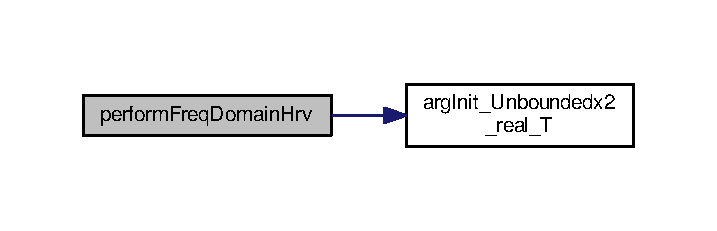
\includegraphics[width=344pt]{group__HRV-Analysis_ga3cfec29967efe1561722a05d03f26158_cgraph}
\end{center}
\end{figure}




Here is the caller graph for this function\+:\nopagebreak
\begin{figure}[H]
\begin{center}
\leavevmode
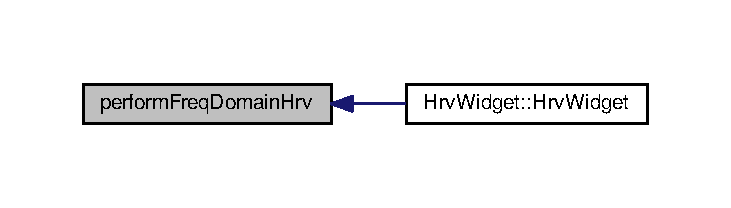
\includegraphics[width=350pt]{group__HRV-Analysis_ga3cfec29967efe1561722a05d03f26158_icgraph}
\end{center}
\end{figure}


\index{H\+R\+V-\/\+Analysis@{H\+R\+V-\/\+Analysis}!perform\+Time\+Domain\+Hrv@{perform\+Time\+Domain\+Hrv}}
\index{perform\+Time\+Domain\+Hrv@{perform\+Time\+Domain\+Hrv}!H\+R\+V-\/\+Analysis@{H\+R\+V-\/\+Analysis}}
\subsubsection[{perform\+Time\+Domain\+Hrv(const Q\+Vector$<$ double $>$ $\ast$ibi\+Data, struct0\+\_\+\+T $\ast$output)}]{\setlength{\rightskip}{0pt plus 5cm}void perform\+Time\+Domain\+Hrv (
\begin{DoxyParamCaption}
\item[{const Q\+Vector$<$ double $>$ $\ast$}]{ibi\+Data, }
\item[{struct0\+\_\+T $\ast$}]{output}
\end{DoxyParamCaption}
)}\hypertarget{group__HRV-Analysis_ga2bd6c358a622e01babb7fdbca313c50f}{}\label{group__HRV-Analysis_ga2bd6c358a622e01babb7fdbca313c50f}


Performs the Statistical Time Domain calculations for H\+RV Analysis. 


\begin{DoxyParams}[1]{Parameters}
\mbox{\tt in}  & {\em ibi\+Data} & Q\+Vector containing double with ibi information. \\
\hline
\mbox{\tt out}  & {\em output} & struct0\+\_\+T containing all the calculated metrics\\
\hline
\end{DoxyParams}
\begin{DoxyRefDesc}{Todo}
\item[\hyperlink{todo__todo000015}{Todo}]Add Ectopic Intervall Detection and Ectopic Interval Correction for the ibi\+Data\end{DoxyRefDesc}


Definition at line \hyperlink{hrvanalysis_8cpp_source_l00034}{34} of file \hyperlink{hrvanalysis_8cpp_source}{hrvanalysis.\+cpp}.



Here is the call graph for this function\+:\nopagebreak
\begin{figure}[H]
\begin{center}
\leavevmode
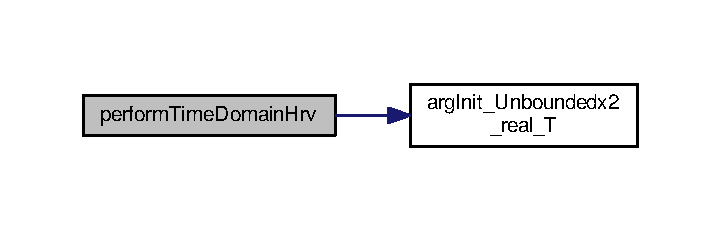
\includegraphics[width=346pt]{group__HRV-Analysis_ga2bd6c358a622e01babb7fdbca313c50f_cgraph}
\end{center}
\end{figure}




Here is the caller graph for this function\+:\nopagebreak
\begin{figure}[H]
\begin{center}
\leavevmode
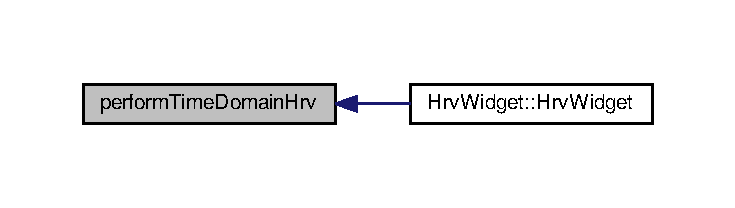
\includegraphics[width=350pt]{group__HRV-Analysis_ga2bd6c358a622e01babb7fdbca313c50f_icgraph}
\end{center}
\end{figure}


\index{H\+R\+V-\/\+Analysis@{H\+R\+V-\/\+Analysis}!Q\+R\+S\+Det@{Q\+R\+S\+Det}}
\index{Q\+R\+S\+Det@{Q\+R\+S\+Det}!H\+R\+V-\/\+Analysis@{H\+R\+V-\/\+Analysis}}
\subsubsection[{Q\+R\+S\+Det(int, int)}]{\setlength{\rightskip}{0pt plus 5cm}int Q\+R\+S\+Det (
\begin{DoxyParamCaption}
\item[{int}]{, }
\item[{int}]{}
\end{DoxyParamCaption}
)}\hypertarget{group__HRV-Analysis_ga5c14f0d7dd58dec49e939470bcb5db1c}{}\label{group__HRV-Analysis_ga5c14f0d7dd58dec49e939470bcb5db1c}


Q\+R\+S\+Det Function used for the Q\+R\+S-\/detection. 

\begin{DoxyReturn}{Returns}

\end{DoxyReturn}


Here is the caller graph for this function\+:\nopagebreak
\begin{figure}[H]
\begin{center}
\leavevmode
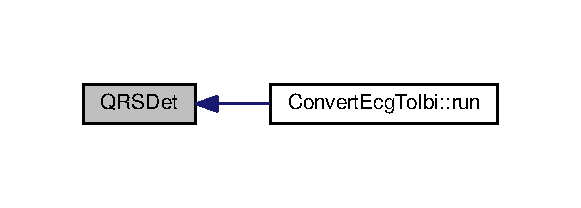
\includegraphics[width=279pt]{group__HRV-Analysis_ga5c14f0d7dd58dec49e939470bcb5db1c_icgraph}
\end{center}
\end{figure}



\hypertarget{group__DataLogger}{}\section{Data\+Logger}
\label{group__DataLogger}\index{Data\+Logger@{Data\+Logger}}


Classes and Functions used to log data, for example saving to txt file or edf file.  


\subsection*{Classes}
\begin{DoxyCompactItemize}
\item 
class \hyperlink{classDataLogger}{Data\+Logger}
\begin{DoxyCompactList}\small\item\em The \hyperlink{classDataLogger}{Data\+Logger} class. \end{DoxyCompactList}\end{DoxyCompactItemize}


\subsection{Detailed Description}
Classes and Functions used to log data, for example saving to txt file or edf file. 

\begin{DoxyAuthor}{Author}
Martin 
\end{DoxyAuthor}

\hypertarget{group__Device-Facade}{}\section{Device-\/\+Facade}
\label{group__Device-Facade}\index{Device-\/\+Facade@{Device-\/\+Facade}}


Module responsible for all connection to the Bio\+Medical Devices used.  


\subsection*{Classes}
\begin{DoxyCompactItemize}
\item 
class \hyperlink{classDeviceInterface}{Device\+Interface}
\begin{DoxyCompactList}\small\item\em Abstract interface for all devices. \end{DoxyCompactList}\item 
class \hyperlink{classDeviceManager}{Device\+Manager}
\begin{DoxyCompactList}\small\item\em Handles which device to connect through the \hyperlink{classDeviceInterface}{Device\+Interface}. \end{DoxyCompactList}\item 
class \hyperlink{classEcgCapture}{Ecg\+Capture}
\begin{DoxyCompactList}\small\item\em Responsible for communication with A\+D\+AS. \end{DoxyCompactList}\item 
class \hyperlink{classEcgMock}{Ecg\+Mock}
\begin{DoxyCompactList}\small\item\em Mock version of an device The \hyperlink{classEcgMock}{Ecg\+Mock} device will return sine and cosine functions as data. \end{DoxyCompactList}\item 
class \hyperlink{classSamplingThread}{Sampling\+Thread}
\begin{DoxyCompactList}\small\item\em \hyperlink{classDeviceInterface}{Device\+Interface} Class responsible for sampling E\+CG. \end{DoxyCompactList}\end{DoxyCompactItemize}
\subsection*{Enumerations}
\begin{DoxyCompactItemize}
\item 
enum \hyperlink{group__Device-Facade_gabf6e5cc9109a573e29add762dc36df9b}{Ecg\+Capture\+::\+Operating\+Mode} \{ \hyperlink{group__Device-Facade_ggabf6e5cc9109a573e29add762dc36df9ba9e4c8f425af52209ee3eb7c466852b22}{Ecg\+Capture\+::ecg\+Capture}, 
\hyperlink{group__Device-Facade_ggabf6e5cc9109a573e29add762dc36df9ba8b349f0786d8e8247f4bc381baa51134}{Ecg\+Capture\+::test\+Tone\+Square}, 
\hyperlink{group__Device-Facade_ggabf6e5cc9109a573e29add762dc36df9ba9ececd6d5264a0e5996556c6697a4f94}{Ecg\+Capture\+::test\+Tone\+Low\+Freq\+Sin}, 
\hyperlink{group__Device-Facade_ggabf6e5cc9109a573e29add762dc36df9ba397d60b89ddb5aaf41d92c617868ed47}{Ecg\+Capture\+::test\+Tone\+High\+Freq\+Sin}
 \}
\item 
enum \hyperlink{group__Device-Facade_gaaf4f7677ca26944edc0f65195b8729f3}{Ecg\+Capture\+::\+Frequency} \{ \hyperlink{group__Device-Facade_ggaaf4f7677ca26944edc0f65195b8729f3acb281025a93800e7ed188605a7375838}{Ecg\+Capture\+::low\+Freq}, 
\hyperlink{group__Device-Facade_ggaaf4f7677ca26944edc0f65195b8729f3a2a968734e734a271ef5a52b83360122a}{Ecg\+Capture\+::mid\+Freq}, 
\hyperlink{group__Device-Facade_ggaaf4f7677ca26944edc0f65195b8729f3abd09d184c2c34f227532a8bc5fb90877}{Ecg\+Capture\+::high\+Freq}
 \}
\item 
enum \hyperlink{group__Device-Facade_ga1750ac59389b67ba4d9d2834dd7c2d9c}{Ecg\+Capture\+::lead\+Format} \{ \hyperlink{group__Device-Facade_gga1750ac59389b67ba4d9d2834dd7c2d9caf7786dce131009aa61ddfed4f8d8639b}{Ecg\+Capture\+::digital}, 
\hyperlink{group__Device-Facade_gga1750ac59389b67ba4d9d2834dd7c2d9ca21cabce4f74afcf79d24897058fdd6b9}{Ecg\+Capture\+::electrode}
 \}
\end{DoxyCompactItemize}
\subsection*{Functions}
\begin{DoxyCompactItemize}
\item 
\hyperlink{group__Device-Facade_gaeef1c0708b94ee82330d6d165a2b5a71}{Ecg\+Capture\+::\+Ecg\+Capture} ()
\item 
void \hyperlink{group__Device-Facade_ga8f080b59e8caab0993bb7ee6b872b6a0}{Ecg\+Capture\+::init} (Operating\+Mode, Frequency)
\begin{DoxyCompactList}\small\item\em Initiate the device by configuring the registers depending on operating mode and sampling frequency. \end{DoxyCompactList}\item 
void \hyperlink{group__Device-Facade_ga9582047c81db34a3cab2bb315fcb1793}{Ecg\+Capture\+::start} ()
\begin{DoxyCompactList}\small\item\em Start capturing frames from the A\+D\+A\+S1000. \end{DoxyCompactList}\item 
void \hyperlink{group__Device-Facade_ga8fef74cdd0296256ab4a700dae2d02a4}{Ecg\+Capture\+::stop} ()
\begin{DoxyCompactList}\small\item\em stop capture \end{DoxyCompactList}\item 
void \hyperlink{group__Device-Facade_ga9f04dad928d472c92229f3f39a8f2445}{Ecg\+Capture\+::test\+Device} ()
\begin{DoxyCompactList}\small\item\em Method used to test if the device is working properly. \end{DoxyCompactList}\item 
const Q\+Vector$<$ double $>$ \hyperlink{group__Device-Facade_ga644ec3752de6ee1e818b5fcd1de5decd}{Ecg\+Capture\+::read\+Frame} ()
\begin{DoxyCompactList}\small\item\em Reads a single frame. \end{DoxyCompactList}\end{DoxyCompactItemize}


\subsection{Detailed Description}
Module responsible for all connection to the Bio\+Medical Devices used. 

\begin{DoxyAuthor}{Author}
Martin 
\end{DoxyAuthor}


\subsection{Enumeration Type Documentation}
\index{Device-\/\+Facade@{Device-\/\+Facade}!Frequency@{Frequency}}
\index{Frequency@{Frequency}!Device-\/\+Facade@{Device-\/\+Facade}}
\subsubsection[{Frequency}]{\setlength{\rightskip}{0pt plus 5cm}enum {\bf Ecg\+Capture\+::\+Frequency}}\hypertarget{group__Device-Facade_gaaf4f7677ca26944edc0f65195b8729f3}{}\label{group__Device-Facade_gaaf4f7677ca26944edc0f65195b8729f3}
\begin{Desc}
\item[Enumerator]\par
\begin{description}
\index{low\+Freq@{low\+Freq}!Device-\/\+Facade@{Device-\/\+Facade}}\index{Device-\/\+Facade@{Device-\/\+Facade}!low\+Freq@{low\+Freq}}\item[{\em 
low\+Freq\hypertarget{group__Device-Facade_ggaaf4f7677ca26944edc0f65195b8729f3acb281025a93800e7ed188605a7375838}{}\label{group__Device-Facade_ggaaf4f7677ca26944edc0f65195b8729f3acb281025a93800e7ed188605a7375838}
}]\index{mid\+Freq@{mid\+Freq}!Device-\/\+Facade@{Device-\/\+Facade}}\index{Device-\/\+Facade@{Device-\/\+Facade}!mid\+Freq@{mid\+Freq}}\item[{\em 
mid\+Freq\hypertarget{group__Device-Facade_ggaaf4f7677ca26944edc0f65195b8729f3a2a968734e734a271ef5a52b83360122a}{}\label{group__Device-Facade_ggaaf4f7677ca26944edc0f65195b8729f3a2a968734e734a271ef5a52b83360122a}
}]\index{high\+Freq@{high\+Freq}!Device-\/\+Facade@{Device-\/\+Facade}}\index{Device-\/\+Facade@{Device-\/\+Facade}!high\+Freq@{high\+Freq}}\item[{\em 
high\+Freq\hypertarget{group__Device-Facade_ggaaf4f7677ca26944edc0f65195b8729f3abd09d184c2c34f227532a8bc5fb90877}{}\label{group__Device-Facade_ggaaf4f7677ca26944edc0f65195b8729f3abd09d184c2c34f227532a8bc5fb90877}
}]\end{description}
\end{Desc}


Definition at line \hyperlink{ecgcapture_8h_source_l00037}{37} of file \hyperlink{ecgcapture_8h_source}{ecgcapture.\+h}.

\index{Device-\/\+Facade@{Device-\/\+Facade}!lead\+Format@{lead\+Format}}
\index{lead\+Format@{lead\+Format}!Device-\/\+Facade@{Device-\/\+Facade}}
\subsubsection[{lead\+Format}]{\setlength{\rightskip}{0pt plus 5cm}enum {\bf Ecg\+Capture\+::lead\+Format}}\hypertarget{group__Device-Facade_ga1750ac59389b67ba4d9d2834dd7c2d9c}{}\label{group__Device-Facade_ga1750ac59389b67ba4d9d2834dd7c2d9c}
\begin{Desc}
\item[Enumerator]\par
\begin{description}
\index{digital@{digital}!Device-\/\+Facade@{Device-\/\+Facade}}\index{Device-\/\+Facade@{Device-\/\+Facade}!digital@{digital}}\item[{\em 
digital\hypertarget{group__Device-Facade_gga1750ac59389b67ba4d9d2834dd7c2d9caf7786dce131009aa61ddfed4f8d8639b}{}\label{group__Device-Facade_gga1750ac59389b67ba4d9d2834dd7c2d9caf7786dce131009aa61ddfed4f8d8639b}
}]\index{electrode@{electrode}!Device-\/\+Facade@{Device-\/\+Facade}}\index{Device-\/\+Facade@{Device-\/\+Facade}!electrode@{electrode}}\item[{\em 
electrode\hypertarget{group__Device-Facade_gga1750ac59389b67ba4d9d2834dd7c2d9ca21cabce4f74afcf79d24897058fdd6b9}{}\label{group__Device-Facade_gga1750ac59389b67ba4d9d2834dd7c2d9ca21cabce4f74afcf79d24897058fdd6b9}
}]\end{description}
\end{Desc}


Definition at line \hyperlink{ecgcapture_8h_source_l00043}{43} of file \hyperlink{ecgcapture_8h_source}{ecgcapture.\+h}.

\index{Device-\/\+Facade@{Device-\/\+Facade}!Operating\+Mode@{Operating\+Mode}}
\index{Operating\+Mode@{Operating\+Mode}!Device-\/\+Facade@{Device-\/\+Facade}}
\subsubsection[{Operating\+Mode}]{\setlength{\rightskip}{0pt plus 5cm}enum {\bf Ecg\+Capture\+::\+Operating\+Mode}}\hypertarget{group__Device-Facade_gabf6e5cc9109a573e29add762dc36df9b}{}\label{group__Device-Facade_gabf6e5cc9109a573e29add762dc36df9b}
\begin{Desc}
\item[Enumerator]\par
\begin{description}
\index{ecg\+Capture@{ecg\+Capture}!Device-\/\+Facade@{Device-\/\+Facade}}\index{Device-\/\+Facade@{Device-\/\+Facade}!ecg\+Capture@{ecg\+Capture}}\item[{\em 
ecg\+Capture\hypertarget{group__Device-Facade_ggabf6e5cc9109a573e29add762dc36df9ba9e4c8f425af52209ee3eb7c466852b22}{}\label{group__Device-Facade_ggabf6e5cc9109a573e29add762dc36df9ba9e4c8f425af52209ee3eb7c466852b22}
}]\index{test\+Tone\+Square@{test\+Tone\+Square}!Device-\/\+Facade@{Device-\/\+Facade}}\index{Device-\/\+Facade@{Device-\/\+Facade}!test\+Tone\+Square@{test\+Tone\+Square}}\item[{\em 
test\+Tone\+Square\hypertarget{group__Device-Facade_ggabf6e5cc9109a573e29add762dc36df9ba8b349f0786d8e8247f4bc381baa51134}{}\label{group__Device-Facade_ggabf6e5cc9109a573e29add762dc36df9ba8b349f0786d8e8247f4bc381baa51134}
}]\index{test\+Tone\+Low\+Freq\+Sin@{test\+Tone\+Low\+Freq\+Sin}!Device-\/\+Facade@{Device-\/\+Facade}}\index{Device-\/\+Facade@{Device-\/\+Facade}!test\+Tone\+Low\+Freq\+Sin@{test\+Tone\+Low\+Freq\+Sin}}\item[{\em 
test\+Tone\+Low\+Freq\+Sin\hypertarget{group__Device-Facade_ggabf6e5cc9109a573e29add762dc36df9ba9ececd6d5264a0e5996556c6697a4f94}{}\label{group__Device-Facade_ggabf6e5cc9109a573e29add762dc36df9ba9ececd6d5264a0e5996556c6697a4f94}
}]\index{test\+Tone\+High\+Freq\+Sin@{test\+Tone\+High\+Freq\+Sin}!Device-\/\+Facade@{Device-\/\+Facade}}\index{Device-\/\+Facade@{Device-\/\+Facade}!test\+Tone\+High\+Freq\+Sin@{test\+Tone\+High\+Freq\+Sin}}\item[{\em 
test\+Tone\+High\+Freq\+Sin\hypertarget{group__Device-Facade_ggabf6e5cc9109a573e29add762dc36df9ba397d60b89ddb5aaf41d92c617868ed47}{}\label{group__Device-Facade_ggabf6e5cc9109a573e29add762dc36df9ba397d60b89ddb5aaf41d92c617868ed47}
}]\end{description}
\end{Desc}


Definition at line \hyperlink{ecgcapture_8h_source_l00030}{30} of file \hyperlink{ecgcapture_8h_source}{ecgcapture.\+h}.



\subsection{Function Documentation}
\index{Device-\/\+Facade@{Device-\/\+Facade}!Ecg\+Capture@{Ecg\+Capture}}
\index{Ecg\+Capture@{Ecg\+Capture}!Device-\/\+Facade@{Device-\/\+Facade}}
\subsubsection[{Ecg\+Capture()}]{\setlength{\rightskip}{0pt plus 5cm}Ecg\+Capture\+::\+Ecg\+Capture (
\begin{DoxyParamCaption}
{}
\end{DoxyParamCaption}
)}\hypertarget{group__Device-Facade_gaeef1c0708b94ee82330d6d165a2b5a71}{}\label{group__Device-Facade_gaeef1c0708b94ee82330d6d165a2b5a71}


Definition at line \hyperlink{ecgcapture_8cpp_source_l00015}{15} of file \hyperlink{ecgcapture_8cpp_source}{ecgcapture.\+cpp}.

\index{Device-\/\+Facade@{Device-\/\+Facade}!init@{init}}
\index{init@{init}!Device-\/\+Facade@{Device-\/\+Facade}}
\subsubsection[{init(\+Operating\+Mode, Frequency)}]{\setlength{\rightskip}{0pt plus 5cm}void Ecg\+Capture\+::init (
\begin{DoxyParamCaption}
\item[{{\bf Operating\+Mode}}]{mode, }
\item[{{\bf Frequency}}]{freq}
\end{DoxyParamCaption}
)}\hypertarget{group__Device-Facade_ga8f080b59e8caab0993bb7ee6b872b6a0}{}\label{group__Device-Facade_ga8f080b59e8caab0993bb7ee6b872b6a0}


Initiate the device by configuring the registers depending on operating mode and sampling frequency. 


\begin{DoxyParams}[1]{Parameters}
\mbox{\tt in}  & {\em Operating\+Mode} & enum stating which operating mode to use \\
\hline
\mbox{\tt in}  & {\em Frequency} & enum stating the which frequency to sample in \\
\hline
\end{DoxyParams}


Definition at line \hyperlink{ecgcapture_8cpp_source_l00026}{26} of file \hyperlink{ecgcapture_8cpp_source}{ecgcapture.\+cpp}.



Here is the caller graph for this function\+:
\nopagebreak
\begin{figure}[H]
\begin{center}
\leavevmode
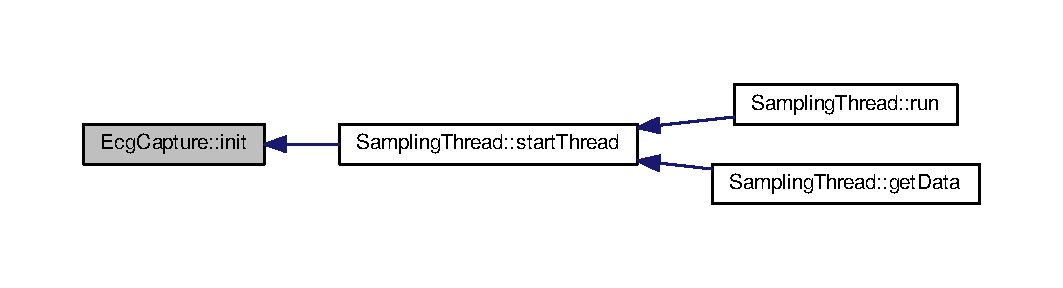
\includegraphics[width=350pt]{group__Device-Facade_ga8f080b59e8caab0993bb7ee6b872b6a0_icgraph}
\end{center}
\end{figure}


\index{Device-\/\+Facade@{Device-\/\+Facade}!read\+Frame@{read\+Frame}}
\index{read\+Frame@{read\+Frame}!Device-\/\+Facade@{Device-\/\+Facade}}
\subsubsection[{read\+Frame()}]{\setlength{\rightskip}{0pt plus 5cm}const Q\+Vector$<$ double $>$ Ecg\+Capture\+::read\+Frame (
\begin{DoxyParamCaption}
{}
\end{DoxyParamCaption}
)}\hypertarget{group__Device-Facade_ga644ec3752de6ee1e818b5fcd1de5decd}{}\label{group__Device-Facade_ga644ec3752de6ee1e818b5fcd1de5decd}


Reads a single frame. 

\begin{DoxyReturn}{Returns}
Q\+Vector$<$double$>$ single\+Frame 
\end{DoxyReturn}


Definition at line \hyperlink{ecgcapture_8cpp_source_l00400}{400} of file \hyperlink{ecgcapture_8cpp_source}{ecgcapture.\+cpp}.



Here is the call graph for this function\+:
\nopagebreak
\begin{figure}[H]
\begin{center}
\leavevmode
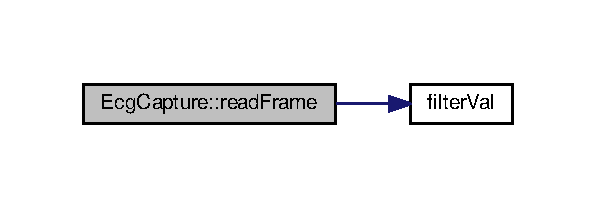
\includegraphics[width=286pt]{group__Device-Facade_ga644ec3752de6ee1e818b5fcd1de5decd_cgraph}
\end{center}
\end{figure}




Here is the caller graph for this function\+:
\nopagebreak
\begin{figure}[H]
\begin{center}
\leavevmode
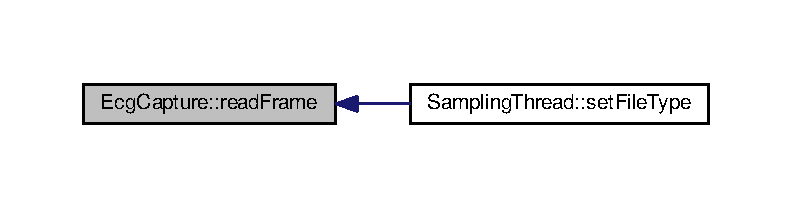
\includegraphics[width=350pt]{group__Device-Facade_ga644ec3752de6ee1e818b5fcd1de5decd_icgraph}
\end{center}
\end{figure}


\index{Device-\/\+Facade@{Device-\/\+Facade}!start@{start}}
\index{start@{start}!Device-\/\+Facade@{Device-\/\+Facade}}
\subsubsection[{start()}]{\setlength{\rightskip}{0pt plus 5cm}void Ecg\+Capture\+::start (
\begin{DoxyParamCaption}
{}
\end{DoxyParamCaption}
)}\hypertarget{group__Device-Facade_ga9582047c81db34a3cab2bb315fcb1793}{}\label{group__Device-Facade_ga9582047c81db34a3cab2bb315fcb1793}


Start capturing frames from the A\+D\+A\+S1000. 

Start sending frames. 

Definition at line \hyperlink{ecgcapture_8cpp_source_l00353}{353} of file \hyperlink{ecgcapture_8cpp_source}{ecgcapture.\+cpp}.



Here is the caller graph for this function\+:
\nopagebreak
\begin{figure}[H]
\begin{center}
\leavevmode
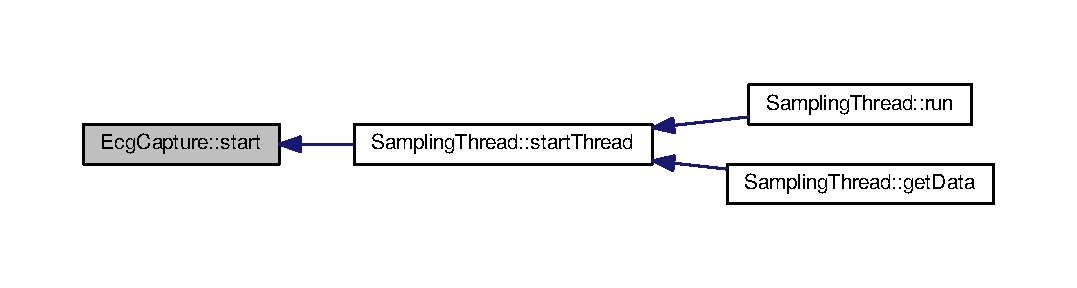
\includegraphics[width=350pt]{group__Device-Facade_ga9582047c81db34a3cab2bb315fcb1793_icgraph}
\end{center}
\end{figure}


\index{Device-\/\+Facade@{Device-\/\+Facade}!stop@{stop}}
\index{stop@{stop}!Device-\/\+Facade@{Device-\/\+Facade}}
\subsubsection[{stop()}]{\setlength{\rightskip}{0pt plus 5cm}void Ecg\+Capture\+::stop (
\begin{DoxyParamCaption}
{}
\end{DoxyParamCaption}
)}\hypertarget{group__Device-Facade_ga8fef74cdd0296256ab4a700dae2d02a4}{}\label{group__Device-Facade_ga8fef74cdd0296256ab4a700dae2d02a4}


stop capture 

\begin{DoxyRefDesc}{Todo}
\item[\hyperlink{todo__todo000012}{Todo}]Implement\end{DoxyRefDesc}


Definition at line \hyperlink{ecgcapture_8cpp_source_l00362}{362} of file \hyperlink{ecgcapture_8cpp_source}{ecgcapture.\+cpp}.

\index{Device-\/\+Facade@{Device-\/\+Facade}!test\+Device@{test\+Device}}
\index{test\+Device@{test\+Device}!Device-\/\+Facade@{Device-\/\+Facade}}
\subsubsection[{test\+Device()}]{\setlength{\rightskip}{0pt plus 5cm}void Ecg\+Capture\+::test\+Device (
\begin{DoxyParamCaption}
{}
\end{DoxyParamCaption}
)}\hypertarget{group__Device-Facade_ga9f04dad928d472c92229f3f39a8f2445}{}\label{group__Device-Facade_ga9f04dad928d472c92229f3f39a8f2445}


Method used to test if the device is working properly. 

It works by writing to a register and then reading the same register.

\begin{DoxyRefDesc}{Deprecated}
\item[\hyperlink{deprecated__deprecated000002}{Deprecated}]Currently not in use. \end{DoxyRefDesc}


Definition at line \hyperlink{ecgcapture_8cpp_source_l00257}{257} of file \hyperlink{ecgcapture_8cpp_source}{ecgcapture.\+cpp}.


\chapter{Namespace Documentation}
\hypertarget{namespaceUi}{}\section{Ui Namespace Reference}
\label{namespaceUi}\index{Ui@{Ui}}

\chapter{Class Documentation}
\hypertarget{classAbstractMenu}{}\section{Abstract\+Menu Class Reference}
\label{classAbstractMenu}\index{Abstract\+Menu@{Abstract\+Menu}}


Abstract menu object for Pi\+Face C\+AD.  




{\ttfamily \#include $<$abstractmenu.\+h$>$}



Inheritance diagram for Abstract\+Menu\+:
\nopagebreak
\begin{figure}[H]
\begin{center}
\leavevmode
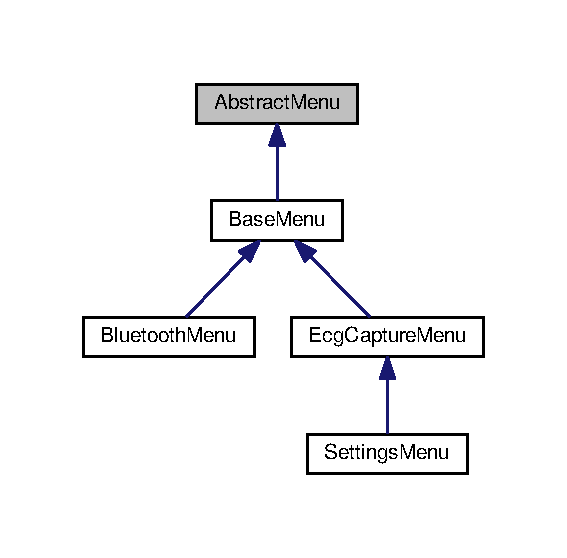
\includegraphics[width=272pt]{classAbstractMenu__inherit__graph}
\end{center}
\end{figure}
\subsection*{Public Member Functions}
\begin{DoxyCompactItemize}
\item 
\hyperlink{classAbstractMenu_a45d32cb02984b79e6bc6f6e930ee5c8c}{Abstract\+Menu} ()
\item 
virtual \hyperlink{classAbstractMenu_af4aacdda3e23fedf1de7781befe22116}{$\sim$\+Abstract\+Menu} ()
\item 
virtual \hyperlink{classAbstractMenu}{Abstract\+Menu} $\ast$ \hyperlink{classAbstractMenu_aef49c4a4ceeb1aad12101cb4768e1596}{new\+Menu} ()=0
\begin{DoxyCompactList}\small\item\em Pure virtual function, creates the next Menu object Pure virtual function, that is meant to create a the \hyperlink{classAbstractMenu}{Abstract\+Menu} object that comes after the Menu\+Object that called it. \end{DoxyCompactList}\item 
virtual void \hyperlink{classAbstractMenu_a4163c42d2127430e184612cb95211cda}{set\+Upper\+Text} ()
\begin{DoxyCompactList}\small\item\em Sets the first row of the Pi\+Face C\+AD to the current option choosen Uses the C library pifacecad.\+h to control the display. \end{DoxyCompactList}\item 
virtual void \hyperlink{classAbstractMenu_ab07feae31d2527f2830188fc10bcb728}{set\+Upper\+Text} (const char $\ast$)
\begin{DoxyCompactList}\small\item\em Sets the first row of the Pi\+Face C\+AD to the current option choosen Uses the C library pifacecad.\+h to control the display. \end{DoxyCompactList}\item 
virtual void \hyperlink{classAbstractMenu_afc9ee4bf101f2761b4e8e083ef3c4a9b}{next} ()
\begin{DoxyCompactList}\small\item\em Toggles the second row of the Pi\+Face C\+AD to the next option Uses the C library pifacecad.\+h to control the display. \end{DoxyCompactList}\item 
virtual void \hyperlink{classAbstractMenu_a5fd1c385e4acd825631ede5bb0424a5c}{set\+Lower\+Text} ()
\begin{DoxyCompactList}\small\item\em Sets the second row of the Pi\+Face C\+AD to the current option choosen Uses the C library pifacecad.\+h to control the display. \end{DoxyCompactList}\end{DoxyCompactItemize}
\subsection*{Protected Attributes}
\begin{DoxyCompactItemize}
\item 
std\+::vector$<$ std\+::string $>$ \hyperlink{classAbstractMenu_a990dc4299fbe86152487fd35d46a403b}{options}
\begin{DoxyCompactList}\small\item\em std\+::vector containing the different options to display on the Pi\+Face C\+AD To be set by the derived \hyperlink{classAbstractMenu}{Abstract\+Menu} object \end{DoxyCompactList}\item 
int \hyperlink{classAbstractMenu_a6caff7f6281c6c2912e5f808c2906123}{number\+Of\+Options}
\begin{DoxyCompactList}\small\item\em number of elements stored in the options vector. To be set by the derived \hyperlink{classAbstractMenu}{Abstract\+Menu} object \end{DoxyCompactList}\item 
int \hyperlink{classAbstractMenu_a589fea1bf68c33e0eff64c8b609cb980}{current\+Option}
\begin{DoxyCompactList}\small\item\em Counter that keeps track of the option visible on the Pi\+Face C\+AD. \end{DoxyCompactList}\end{DoxyCompactItemize}


\subsection{Detailed Description}
Abstract menu object for Pi\+Face C\+AD. 

\hyperlink{classAbstractMenu}{Abstract\+Menu} is the base class for menu objects to be used to create a small logical menu that can be called from the Pi\+Face C\+AD

\begin{DoxyAuthor}{Author}
Martin 
\end{DoxyAuthor}


Definition at line \hyperlink{abstractmenu_8h_source_l00017}{17} of file \hyperlink{abstractmenu_8h_source}{abstractmenu.\+h}.



\subsection{Constructor \& Destructor Documentation}
\index{Abstract\+Menu@{Abstract\+Menu}!Abstract\+Menu@{Abstract\+Menu}}
\index{Abstract\+Menu@{Abstract\+Menu}!Abstract\+Menu@{Abstract\+Menu}}
\subsubsection[{Abstract\+Menu()}]{\setlength{\rightskip}{0pt plus 5cm}Abstract\+Menu\+::\+Abstract\+Menu (
\begin{DoxyParamCaption}
{}
\end{DoxyParamCaption}
)}\hypertarget{classAbstractMenu_a45d32cb02984b79e6bc6f6e930ee5c8c}{}\label{classAbstractMenu_a45d32cb02984b79e6bc6f6e930ee5c8c}


Definition at line \hyperlink{abstractmenu_8cpp_source_l00004}{4} of file \hyperlink{abstractmenu_8cpp_source}{abstractmenu.\+cpp}.

\index{Abstract\+Menu@{Abstract\+Menu}!````~Abstract\+Menu@{$\sim$\+Abstract\+Menu}}
\index{````~Abstract\+Menu@{$\sim$\+Abstract\+Menu}!Abstract\+Menu@{Abstract\+Menu}}
\subsubsection[{$\sim$\+Abstract\+Menu()}]{\setlength{\rightskip}{0pt plus 5cm}virtual Abstract\+Menu\+::$\sim$\+Abstract\+Menu (
\begin{DoxyParamCaption}
{}
\end{DoxyParamCaption}
)\hspace{0.3cm}{\ttfamily [inline]}, {\ttfamily [virtual]}}\hypertarget{classAbstractMenu_af4aacdda3e23fedf1de7781befe22116}{}\label{classAbstractMenu_af4aacdda3e23fedf1de7781befe22116}


Definition at line \hyperlink{abstractmenu_8h_source_l00021}{21} of file \hyperlink{abstractmenu_8h_source}{abstractmenu.\+h}.



Here is the call graph for this function\+:
\nopagebreak
\begin{figure}[H]
\begin{center}
\leavevmode
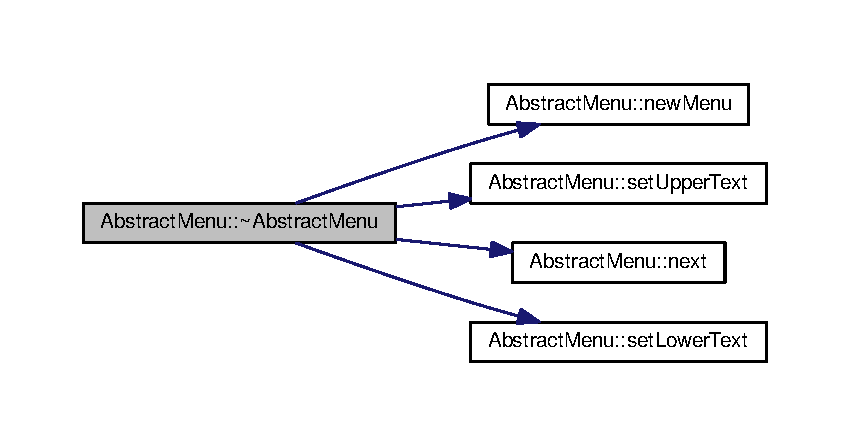
\includegraphics[width=350pt]{classAbstractMenu_af4aacdda3e23fedf1de7781befe22116_cgraph}
\end{center}
\end{figure}




\subsection{Member Function Documentation}
\index{Abstract\+Menu@{Abstract\+Menu}!new\+Menu@{new\+Menu}}
\index{new\+Menu@{new\+Menu}!Abstract\+Menu@{Abstract\+Menu}}
\subsubsection[{new\+Menu()=0}]{\setlength{\rightskip}{0pt plus 5cm}virtual {\bf Abstract\+Menu}$\ast$ Abstract\+Menu\+::new\+Menu (
\begin{DoxyParamCaption}
{}
\end{DoxyParamCaption}
)\hspace{0.3cm}{\ttfamily [pure virtual]}}\hypertarget{classAbstractMenu_aef49c4a4ceeb1aad12101cb4768e1596}{}\label{classAbstractMenu_aef49c4a4ceeb1aad12101cb4768e1596}


Pure virtual function, creates the next Menu object Pure virtual function, that is meant to create a the \hyperlink{classAbstractMenu}{Abstract\+Menu} object that comes after the Menu\+Object that called it. 

What \hyperlink{classAbstractMenu}{Abstract\+Menu} object that are created depends on in which object the function was called.


\begin{DoxyParams}{Parameters}
{\em current\+Option} & inherited from \hyperlink{classAbstractMenu}{Abstract\+Menu} to realize what Object to create. \\
\hline
\end{DoxyParams}


Implemented in \hyperlink{classEcgCaptureMenu_a610d2985e09cd56cb381e6e443dbbc72}{Ecg\+Capture\+Menu}, \hyperlink{classBluetoothMenu_a0fd16ad5a39ce3624613ad7834a55565}{Bluetooth\+Menu}, \hyperlink{classSettingsMenu_abc441c12e8044c13f1a99791e2ee30d1}{Settings\+Menu}, and \hyperlink{classBaseMenu_a722bb88987e9a64015c59f3419d89704}{Base\+Menu}.



Here is the caller graph for this function\+:
\nopagebreak
\begin{figure}[H]
\begin{center}
\leavevmode
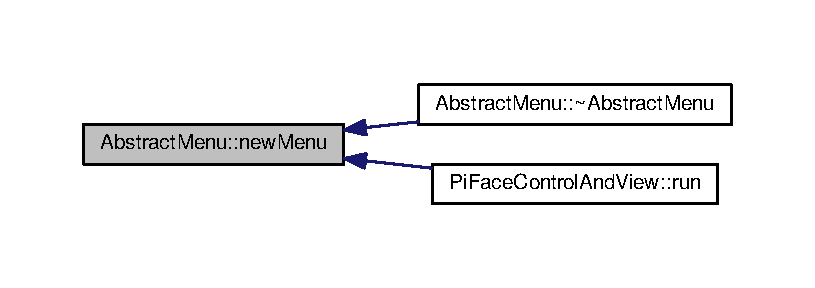
\includegraphics[width=350pt]{classAbstractMenu_aef49c4a4ceeb1aad12101cb4768e1596_icgraph}
\end{center}
\end{figure}


\index{Abstract\+Menu@{Abstract\+Menu}!next@{next}}
\index{next@{next}!Abstract\+Menu@{Abstract\+Menu}}
\subsubsection[{next()}]{\setlength{\rightskip}{0pt plus 5cm}void Abstract\+Menu\+::next (
\begin{DoxyParamCaption}
{}
\end{DoxyParamCaption}
)\hspace{0.3cm}{\ttfamily [virtual]}}\hypertarget{classAbstractMenu_afc9ee4bf101f2761b4e8e083ef3c4a9b}{}\label{classAbstractMenu_afc9ee4bf101f2761b4e8e083ef3c4a9b}


Toggles the second row of the Pi\+Face C\+AD to the next option Uses the C library pifacecad.\+h to control the display. 



Definition at line \hyperlink{abstractmenu_8cpp_source_l00027}{27} of file \hyperlink{abstractmenu_8cpp_source}{abstractmenu.\+cpp}.



Here is the caller graph for this function\+:
\nopagebreak
\begin{figure}[H]
\begin{center}
\leavevmode
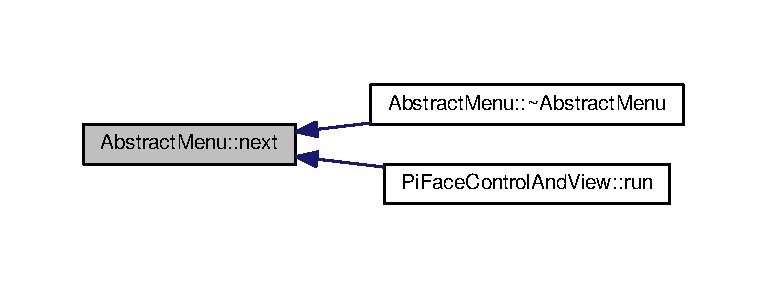
\includegraphics[width=350pt]{classAbstractMenu_afc9ee4bf101f2761b4e8e083ef3c4a9b_icgraph}
\end{center}
\end{figure}


\index{Abstract\+Menu@{Abstract\+Menu}!set\+Lower\+Text@{set\+Lower\+Text}}
\index{set\+Lower\+Text@{set\+Lower\+Text}!Abstract\+Menu@{Abstract\+Menu}}
\subsubsection[{set\+Lower\+Text()}]{\setlength{\rightskip}{0pt plus 5cm}void Abstract\+Menu\+::set\+Lower\+Text (
\begin{DoxyParamCaption}
{}
\end{DoxyParamCaption}
)\hspace{0.3cm}{\ttfamily [virtual]}}\hypertarget{classAbstractMenu_a5fd1c385e4acd825631ede5bb0424a5c}{}\label{classAbstractMenu_a5fd1c385e4acd825631ede5bb0424a5c}


Sets the second row of the Pi\+Face C\+AD to the current option choosen Uses the C library pifacecad.\+h to control the display. 



Definition at line \hyperlink{abstractmenu_8cpp_source_l00021}{21} of file \hyperlink{abstractmenu_8cpp_source}{abstractmenu.\+cpp}.



Here is the caller graph for this function\+:
\nopagebreak
\begin{figure}[H]
\begin{center}
\leavevmode
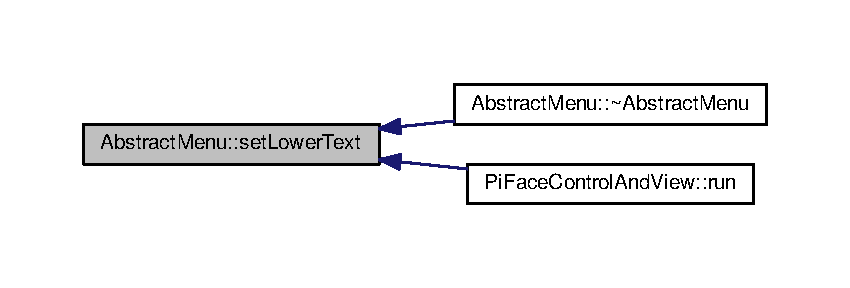
\includegraphics[width=350pt]{classAbstractMenu_a5fd1c385e4acd825631ede5bb0424a5c_icgraph}
\end{center}
\end{figure}


\index{Abstract\+Menu@{Abstract\+Menu}!set\+Upper\+Text@{set\+Upper\+Text}}
\index{set\+Upper\+Text@{set\+Upper\+Text}!Abstract\+Menu@{Abstract\+Menu}}
\subsubsection[{set\+Upper\+Text()}]{\setlength{\rightskip}{0pt plus 5cm}void Abstract\+Menu\+::set\+Upper\+Text (
\begin{DoxyParamCaption}
{}
\end{DoxyParamCaption}
)\hspace{0.3cm}{\ttfamily [virtual]}}\hypertarget{classAbstractMenu_a4163c42d2127430e184612cb95211cda}{}\label{classAbstractMenu_a4163c42d2127430e184612cb95211cda}


Sets the first row of the Pi\+Face C\+AD to the current option choosen Uses the C library pifacecad.\+h to control the display. 



Definition at line \hyperlink{abstractmenu_8cpp_source_l00009}{9} of file \hyperlink{abstractmenu_8cpp_source}{abstractmenu.\+cpp}.



Here is the caller graph for this function\+:
\nopagebreak
\begin{figure}[H]
\begin{center}
\leavevmode
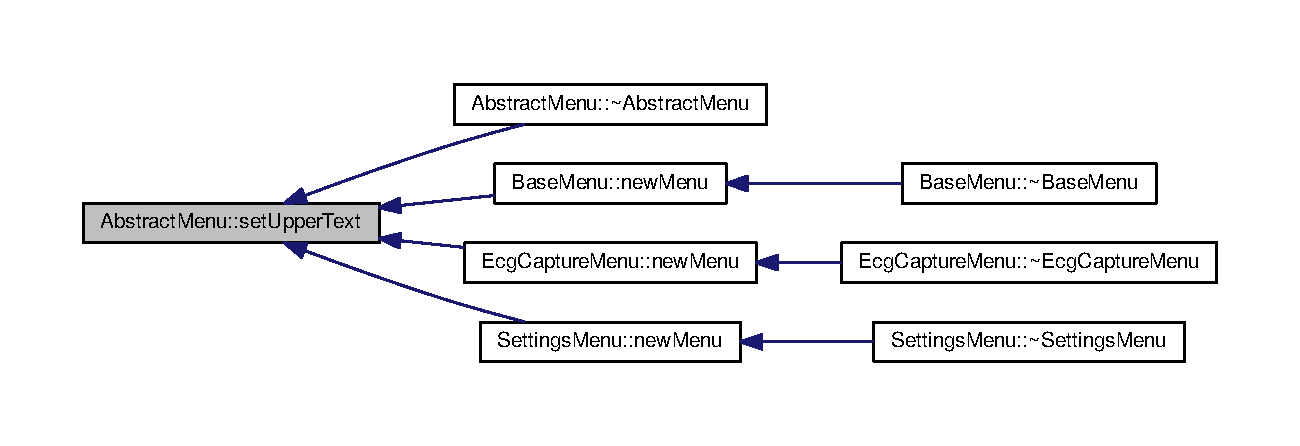
\includegraphics[width=350pt]{classAbstractMenu_a4163c42d2127430e184612cb95211cda_icgraph}
\end{center}
\end{figure}


\index{Abstract\+Menu@{Abstract\+Menu}!set\+Upper\+Text@{set\+Upper\+Text}}
\index{set\+Upper\+Text@{set\+Upper\+Text}!Abstract\+Menu@{Abstract\+Menu}}
\subsubsection[{set\+Upper\+Text(const char $\ast$)}]{\setlength{\rightskip}{0pt plus 5cm}void Abstract\+Menu\+::set\+Upper\+Text (
\begin{DoxyParamCaption}
\item[{const char $\ast$}]{input}
\end{DoxyParamCaption}
)\hspace{0.3cm}{\ttfamily [virtual]}}\hypertarget{classAbstractMenu_ab07feae31d2527f2830188fc10bcb728}{}\label{classAbstractMenu_ab07feae31d2527f2830188fc10bcb728}


Sets the first row of the Pi\+Face C\+AD to the current option choosen Uses the C library pifacecad.\+h to control the display. 


\begin{DoxyParams}{Parameters}
{\em text} & to display on upper row of Pi\+Face C\+AD \\
\hline
\end{DoxyParams}


Definition at line \hyperlink{abstractmenu_8cpp_source_l00015}{15} of file \hyperlink{abstractmenu_8cpp_source}{abstractmenu.\+cpp}.



\subsection{Member Data Documentation}
\index{Abstract\+Menu@{Abstract\+Menu}!current\+Option@{current\+Option}}
\index{current\+Option@{current\+Option}!Abstract\+Menu@{Abstract\+Menu}}
\subsubsection[{current\+Option}]{\setlength{\rightskip}{0pt plus 5cm}int Abstract\+Menu\+::current\+Option\hspace{0.3cm}{\ttfamily [protected]}}\hypertarget{classAbstractMenu_a589fea1bf68c33e0eff64c8b609cb980}{}\label{classAbstractMenu_a589fea1bf68c33e0eff64c8b609cb980}


Counter that keeps track of the option visible on the Pi\+Face C\+AD. 


\begin{DoxyParams}{Parameters}
{\em current\+Option} & \\
\hline
\end{DoxyParams}


Definition at line \hyperlink{abstractmenu_8h_source_l00082}{82} of file \hyperlink{abstractmenu_8h_source}{abstractmenu.\+h}.

\index{Abstract\+Menu@{Abstract\+Menu}!number\+Of\+Options@{number\+Of\+Options}}
\index{number\+Of\+Options@{number\+Of\+Options}!Abstract\+Menu@{Abstract\+Menu}}
\subsubsection[{number\+Of\+Options}]{\setlength{\rightskip}{0pt plus 5cm}int Abstract\+Menu\+::number\+Of\+Options\hspace{0.3cm}{\ttfamily [protected]}}\hypertarget{classAbstractMenu_a6caff7f6281c6c2912e5f808c2906123}{}\label{classAbstractMenu_a6caff7f6281c6c2912e5f808c2906123}


number of elements stored in the options vector. To be set by the derived \hyperlink{classAbstractMenu}{Abstract\+Menu} object 


\begin{DoxyParams}{Parameters}
{\em number\+Of\+Options} & \\
\hline
\end{DoxyParams}


Definition at line \hyperlink{abstractmenu_8h_source_l00076}{76} of file \hyperlink{abstractmenu_8h_source}{abstractmenu.\+h}.

\index{Abstract\+Menu@{Abstract\+Menu}!options@{options}}
\index{options@{options}!Abstract\+Menu@{Abstract\+Menu}}
\subsubsection[{options}]{\setlength{\rightskip}{0pt plus 5cm}std\+::vector$<$std\+::string$>$ Abstract\+Menu\+::options\hspace{0.3cm}{\ttfamily [protected]}}\hypertarget{classAbstractMenu_a990dc4299fbe86152487fd35d46a403b}{}\label{classAbstractMenu_a990dc4299fbe86152487fd35d46a403b}


std\+::vector containing the different options to display on the Pi\+Face C\+AD To be set by the derived \hyperlink{classAbstractMenu}{Abstract\+Menu} object 


\begin{DoxyParams}{Parameters}
{\em options} & \\
\hline
\end{DoxyParams}


Definition at line \hyperlink{abstractmenu_8h_source_l00070}{70} of file \hyperlink{abstractmenu_8h_source}{abstractmenu.\+h}.



The documentation for this class was generated from the following files\+:\begin{DoxyCompactItemize}
\item 
src/\+Pi\+Face-\/\+Interface/\hyperlink{abstractmenu_8h}{abstractmenu.\+h}\item 
src/\+Pi\+Face-\/\+Interface/\hyperlink{abstractmenu_8cpp}{abstractmenu.\+cpp}\end{DoxyCompactItemize}

\hypertarget{classBaseMenu}{}\section{Base\+Menu Class Reference}
\label{classBaseMenu}\index{Base\+Menu@{Base\+Menu}}


Homepage of the Menu-\/system for the Pi\+Face G\+UI.  




{\ttfamily \#include $<$basemenu.\+h$>$}



Inheritance diagram for Base\+Menu\+:\nopagebreak
\begin{figure}[H]
\begin{center}
\leavevmode
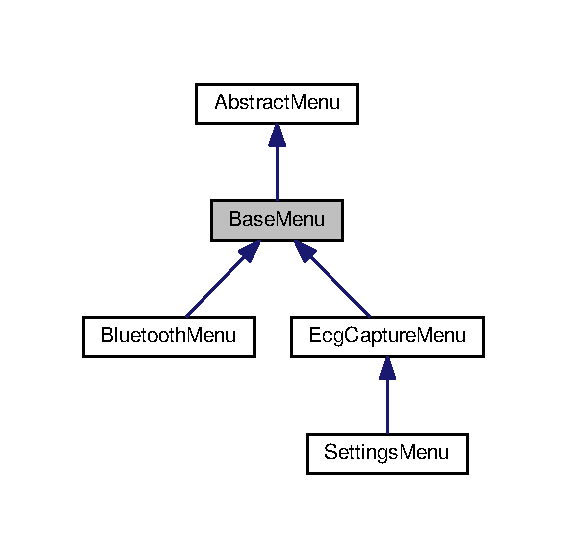
\includegraphics[width=272pt]{classBaseMenu__inherit__graph}
\end{center}
\end{figure}


Collaboration diagram for Base\+Menu\+:\nopagebreak
\begin{figure}[H]
\begin{center}
\leavevmode
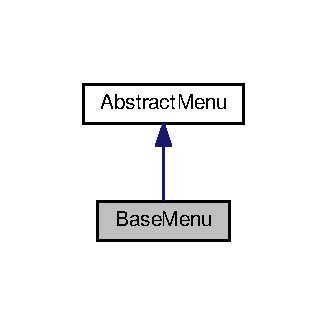
\includegraphics[width=157pt]{classBaseMenu__coll__graph}
\end{center}
\end{figure}
\subsection*{Public Member Functions}
\begin{DoxyCompactItemize}
\item 
\hyperlink{classBaseMenu_aac7431fdaecc0ecc3a0695511dc8426f}{Base\+Menu} ()
\item 
virtual \hyperlink{classBaseMenu_aea8cd4859286c711abee5f54d608cf1a}{$\sim$\+Base\+Menu} ()
\item 
virtual \hyperlink{classAbstractMenu}{Abstract\+Menu} $\ast$ \hyperlink{classBaseMenu_a722bb88987e9a64015c59f3419d89704}{new\+Menu} ()
\begin{DoxyCompactList}\small\item\em Pure virtual function, creates the next Menu object Pure virtual function, that is meant to create a the \hyperlink{classAbstractMenu}{Abstract\+Menu} object that comes after the Menu\+Object that called it. \end{DoxyCompactList}\end{DoxyCompactItemize}
\subsection*{Additional Inherited Members}


\subsection{Detailed Description}
Homepage of the Menu-\/system for the Pi\+Face G\+UI. 

\begin{DoxyAuthor}{Author}
Martin 
\end{DoxyAuthor}


Definition at line \hyperlink{basemenu_8h_source_l00009}{9} of file \hyperlink{basemenu_8h_source}{basemenu.\+h}.



\subsection{Constructor \& Destructor Documentation}
\index{Base\+Menu@{Base\+Menu}!Base\+Menu@{Base\+Menu}}
\index{Base\+Menu@{Base\+Menu}!Base\+Menu@{Base\+Menu}}
\subsubsection[{Base\+Menu()}]{\setlength{\rightskip}{0pt plus 5cm}Base\+Menu\+::\+Base\+Menu (
\begin{DoxyParamCaption}
{}
\end{DoxyParamCaption}
)}\hypertarget{classBaseMenu_aac7431fdaecc0ecc3a0695511dc8426f}{}\label{classBaseMenu_aac7431fdaecc0ecc3a0695511dc8426f}


Definition at line \hyperlink{basemenu_8cpp_source_l00005}{5} of file \hyperlink{basemenu_8cpp_source}{basemenu.\+cpp}.



Here is the caller graph for this function\+:\nopagebreak
\begin{figure}[H]
\begin{center}
\leavevmode
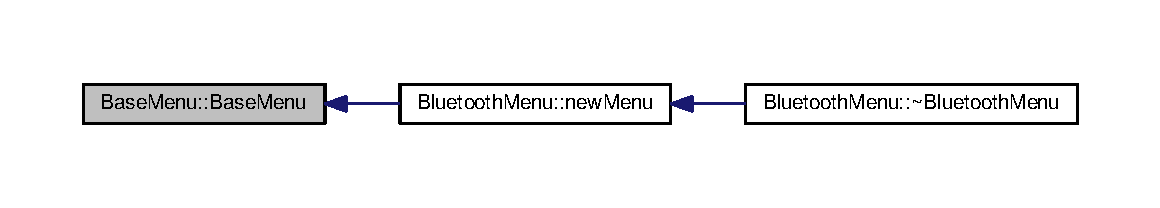
\includegraphics[width=350pt]{classBaseMenu_aac7431fdaecc0ecc3a0695511dc8426f_icgraph}
\end{center}
\end{figure}


\index{Base\+Menu@{Base\+Menu}!````~Base\+Menu@{$\sim$\+Base\+Menu}}
\index{````~Base\+Menu@{$\sim$\+Base\+Menu}!Base\+Menu@{Base\+Menu}}
\subsubsection[{$\sim$\+Base\+Menu()}]{\setlength{\rightskip}{0pt plus 5cm}virtual Base\+Menu\+::$\sim$\+Base\+Menu (
\begin{DoxyParamCaption}
{}
\end{DoxyParamCaption}
)\hspace{0.3cm}{\ttfamily [inline]}, {\ttfamily [virtual]}}\hypertarget{classBaseMenu_aea8cd4859286c711abee5f54d608cf1a}{}\label{classBaseMenu_aea8cd4859286c711abee5f54d608cf1a}


Definition at line \hyperlink{basemenu_8h_source_l00013}{13} of file \hyperlink{basemenu_8h_source}{basemenu.\+h}.



Here is the call graph for this function\+:\nopagebreak
\begin{figure}[H]
\begin{center}
\leavevmode
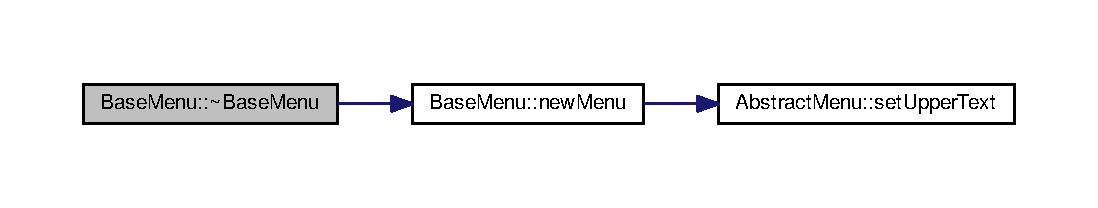
\includegraphics[width=350pt]{classBaseMenu_aea8cd4859286c711abee5f54d608cf1a_cgraph}
\end{center}
\end{figure}




\subsection{Member Function Documentation}
\index{Base\+Menu@{Base\+Menu}!new\+Menu@{new\+Menu}}
\index{new\+Menu@{new\+Menu}!Base\+Menu@{Base\+Menu}}
\subsubsection[{new\+Menu()}]{\setlength{\rightskip}{0pt plus 5cm}{\bf Abstract\+Menu} $\ast$ Base\+Menu\+::new\+Menu (
\begin{DoxyParamCaption}
{}
\end{DoxyParamCaption}
)\hspace{0.3cm}{\ttfamily [virtual]}}\hypertarget{classBaseMenu_a722bb88987e9a64015c59f3419d89704}{}\label{classBaseMenu_a722bb88987e9a64015c59f3419d89704}


Pure virtual function, creates the next Menu object Pure virtual function, that is meant to create a the \hyperlink{classAbstractMenu}{Abstract\+Menu} object that comes after the Menu\+Object that called it. 

What \hyperlink{classAbstractMenu}{Abstract\+Menu} object that are created depends on in which object the function was called.


\begin{DoxyParams}{Parameters}
{\em current\+Option} & inherited from \hyperlink{classAbstractMenu}{Abstract\+Menu} to realize what Object to create. \\
\hline
\end{DoxyParams}


Implements \hyperlink{classAbstractMenu_aef49c4a4ceeb1aad12101cb4768e1596}{Abstract\+Menu}.



Reimplemented in \hyperlink{classEcgCaptureMenu_a610d2985e09cd56cb381e6e443dbbc72}{Ecg\+Capture\+Menu}, \hyperlink{classBluetoothMenu_a0fd16ad5a39ce3624613ad7834a55565}{Bluetooth\+Menu}, and \hyperlink{classSettingsMenu_abc441c12e8044c13f1a99791e2ee30d1}{Settings\+Menu}.



Definition at line \hyperlink{basemenu_8cpp_source_l00011}{11} of file \hyperlink{basemenu_8cpp_source}{basemenu.\+cpp}.



Here is the call graph for this function\+:\nopagebreak
\begin{figure}[H]
\begin{center}
\leavevmode
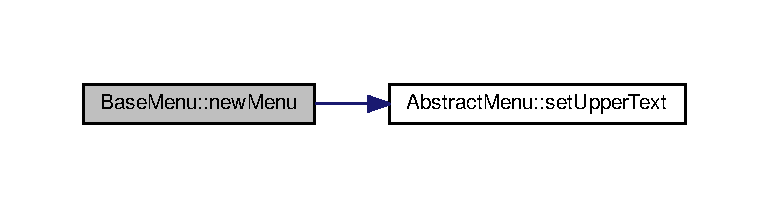
\includegraphics[width=350pt]{classBaseMenu_a722bb88987e9a64015c59f3419d89704_cgraph}
\end{center}
\end{figure}




Here is the caller graph for this function\+:\nopagebreak
\begin{figure}[H]
\begin{center}
\leavevmode
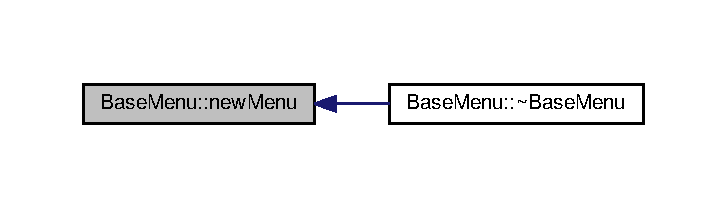
\includegraphics[width=349pt]{classBaseMenu_a722bb88987e9a64015c59f3419d89704_icgraph}
\end{center}
\end{figure}




The documentation for this class was generated from the following files\+:\begin{DoxyCompactItemize}
\item 
src/\+Pi\+Face-\/\+Interface/\hyperlink{basemenu_8h}{basemenu.\+h}\item 
src/\+Pi\+Face-\/\+Interface/\hyperlink{basemenu_8cpp}{basemenu.\+cpp}\end{DoxyCompactItemize}

\hypertarget{classBluetoothMenu}{}\section{Bluetooth\+Menu Class Reference}
\label{classBluetoothMenu}\index{Bluetooth\+Menu@{Bluetooth\+Menu}}


The \hyperlink{classBluetoothMenu}{Bluetooth\+Menu} class.  




{\ttfamily \#include $<$bluetoothmenu.\+h$>$}



Inheritance diagram for Bluetooth\+Menu\+:\nopagebreak
\begin{figure}[H]
\begin{center}
\leavevmode
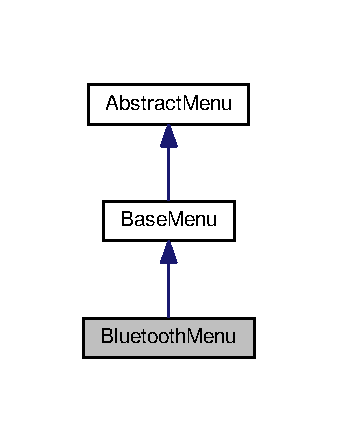
\includegraphics[width=162pt]{classBluetoothMenu__inherit__graph}
\end{center}
\end{figure}


Collaboration diagram for Bluetooth\+Menu\+:\nopagebreak
\begin{figure}[H]
\begin{center}
\leavevmode
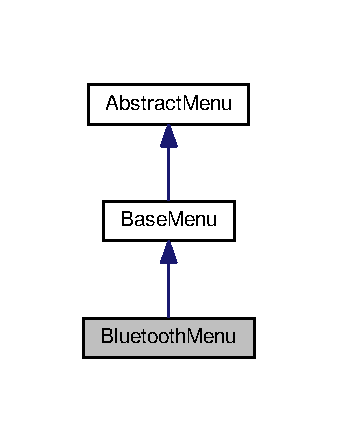
\includegraphics[width=162pt]{classBluetoothMenu__coll__graph}
\end{center}
\end{figure}
\subsection*{Public Member Functions}
\begin{DoxyCompactItemize}
\item 
\hyperlink{classBluetoothMenu_a164151dbccd288a092ddd35f23dfd778}{Bluetooth\+Menu} ()
\item 
virtual \hyperlink{classBluetoothMenu_aa8665ebed9b5bdb0fb9bcb83346ef1ce}{$\sim$\+Bluetooth\+Menu} ()
\item 
virtual \hyperlink{classAbstractMenu}{Abstract\+Menu} $\ast$ \hyperlink{classBluetoothMenu_a0fd16ad5a39ce3624613ad7834a55565}{new\+Menu} ()
\begin{DoxyCompactList}\small\item\em Does nothing. \end{DoxyCompactList}\end{DoxyCompactItemize}
\subsection*{Additional Inherited Members}


\subsection{Detailed Description}
The \hyperlink{classBluetoothMenu}{Bluetooth\+Menu} class. 

\begin{DoxyAuthor}{Author}
Martin 
\end{DoxyAuthor}


Definition at line \hyperlink{bluetoothmenu_8h_source_l00010}{10} of file \hyperlink{bluetoothmenu_8h_source}{bluetoothmenu.\+h}.



\subsection{Constructor \& Destructor Documentation}
\index{Bluetooth\+Menu@{Bluetooth\+Menu}!Bluetooth\+Menu@{Bluetooth\+Menu}}
\index{Bluetooth\+Menu@{Bluetooth\+Menu}!Bluetooth\+Menu@{Bluetooth\+Menu}}
\subsubsection[{Bluetooth\+Menu()}]{\setlength{\rightskip}{0pt plus 5cm}Bluetooth\+Menu\+::\+Bluetooth\+Menu (
\begin{DoxyParamCaption}
{}
\end{DoxyParamCaption}
)}\hypertarget{classBluetoothMenu_a164151dbccd288a092ddd35f23dfd778}{}\label{classBluetoothMenu_a164151dbccd288a092ddd35f23dfd778}


Definition at line \hyperlink{bluetoothmenu_8cpp_source_l00004}{4} of file \hyperlink{bluetoothmenu_8cpp_source}{bluetoothmenu.\+cpp}.

\index{Bluetooth\+Menu@{Bluetooth\+Menu}!````~Bluetooth\+Menu@{$\sim$\+Bluetooth\+Menu}}
\index{````~Bluetooth\+Menu@{$\sim$\+Bluetooth\+Menu}!Bluetooth\+Menu@{Bluetooth\+Menu}}
\subsubsection[{$\sim$\+Bluetooth\+Menu()}]{\setlength{\rightskip}{0pt plus 5cm}virtual Bluetooth\+Menu\+::$\sim$\+Bluetooth\+Menu (
\begin{DoxyParamCaption}
{}
\end{DoxyParamCaption}
)\hspace{0.3cm}{\ttfamily [inline]}, {\ttfamily [virtual]}}\hypertarget{classBluetoothMenu_aa8665ebed9b5bdb0fb9bcb83346ef1ce}{}\label{classBluetoothMenu_aa8665ebed9b5bdb0fb9bcb83346ef1ce}


Definition at line \hyperlink{bluetoothmenu_8h_source_l00014}{14} of file \hyperlink{bluetoothmenu_8h_source}{bluetoothmenu.\+h}.



Here is the call graph for this function\+:\nopagebreak
\begin{figure}[H]
\begin{center}
\leavevmode
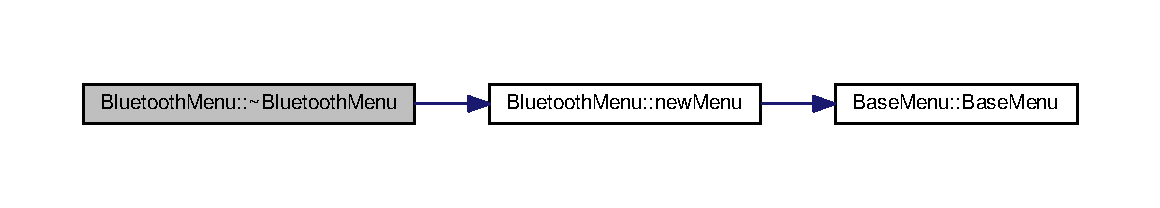
\includegraphics[width=350pt]{classBluetoothMenu_aa8665ebed9b5bdb0fb9bcb83346ef1ce_cgraph}
\end{center}
\end{figure}




\subsection{Member Function Documentation}
\index{Bluetooth\+Menu@{Bluetooth\+Menu}!new\+Menu@{new\+Menu}}
\index{new\+Menu@{new\+Menu}!Bluetooth\+Menu@{Bluetooth\+Menu}}
\subsubsection[{new\+Menu()}]{\setlength{\rightskip}{0pt plus 5cm}{\bf Abstract\+Menu} $\ast$ Bluetooth\+Menu\+::new\+Menu (
\begin{DoxyParamCaption}
{}
\end{DoxyParamCaption}
)\hspace{0.3cm}{\ttfamily [virtual]}}\hypertarget{classBluetoothMenu_a0fd16ad5a39ce3624613ad7834a55565}{}\label{classBluetoothMenu_a0fd16ad5a39ce3624613ad7834a55565}


Does nothing. 

\begin{DoxyRefDesc}{Todo}
\item[\hyperlink{todo__todo000021}{Todo}]implement when Bluetooth functionallity is working for the R\+PI \end{DoxyRefDesc}


\begin{DoxyRefDesc}{Todo}
\item[\hyperlink{todo__todo000020}{Todo}]Implement to get Bluyetooth functionallity \end{DoxyRefDesc}


Reimplemented from \hyperlink{classBaseMenu_a722bb88987e9a64015c59f3419d89704}{Base\+Menu}.



Definition at line \hyperlink{bluetoothmenu_8cpp_source_l00014}{14} of file \hyperlink{bluetoothmenu_8cpp_source}{bluetoothmenu.\+cpp}.



Here is the call graph for this function\+:\nopagebreak
\begin{figure}[H]
\begin{center}
\leavevmode
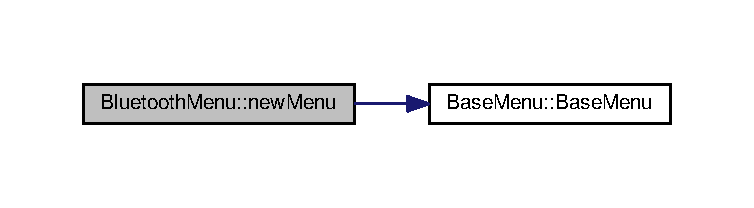
\includegraphics[width=350pt]{classBluetoothMenu_a0fd16ad5a39ce3624613ad7834a55565_cgraph}
\end{center}
\end{figure}




Here is the caller graph for this function\+:\nopagebreak
\begin{figure}[H]
\begin{center}
\leavevmode
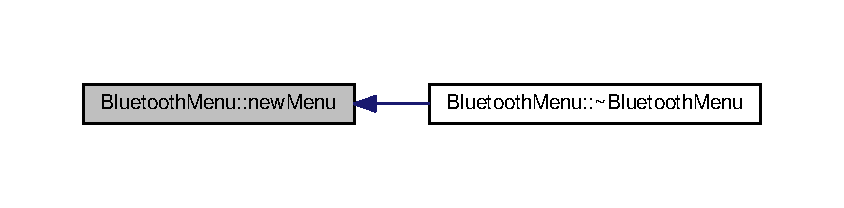
\includegraphics[width=350pt]{classBluetoothMenu_a0fd16ad5a39ce3624613ad7834a55565_icgraph}
\end{center}
\end{figure}




The documentation for this class was generated from the following files\+:\begin{DoxyCompactItemize}
\item 
src/\+Pi\+Face-\/\+Interface/\hyperlink{bluetoothmenu_8h}{bluetoothmenu.\+h}\item 
src/\+Pi\+Face-\/\+Interface/\hyperlink{bluetoothmenu_8cpp}{bluetoothmenu.\+cpp}\end{DoxyCompactItemize}

\hypertarget{classConvertEcgToIbi}{}\section{Convert\+Ecg\+To\+Ibi Class Reference}
\label{classConvertEcgToIbi}\index{Convert\+Ecg\+To\+Ibi@{Convert\+Ecg\+To\+Ibi}}


Converts textfile with E\+C\+G-\/data into I\+BI file.  




{\ttfamily \#include $<$convertecgtoibi.\+h$>$}



Inheritance diagram for Convert\+Ecg\+To\+Ibi\+:\nopagebreak
\begin{figure}[H]
\begin{center}
\leavevmode
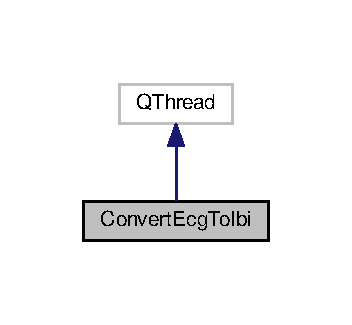
\includegraphics[width=169pt]{classConvertEcgToIbi__inherit__graph}
\end{center}
\end{figure}


Collaboration diagram for Convert\+Ecg\+To\+Ibi\+:\nopagebreak
\begin{figure}[H]
\begin{center}
\leavevmode
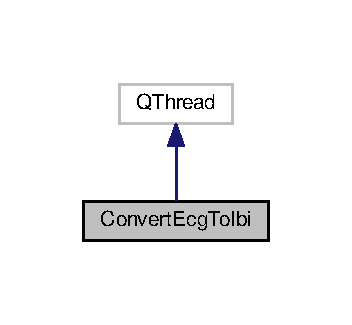
\includegraphics[width=169pt]{classConvertEcgToIbi__coll__graph}
\end{center}
\end{figure}
\subsection*{Signals}
\begin{DoxyCompactItemize}
\item 
void \hyperlink{classConvertEcgToIbi_a34d6d61a81e88116c65a2ba9198b7f1c}{send\+File\+Data} (Q\+Vector$<$ double $>$ qrs\+Peaks, Q\+Vector$<$ double $>$ time\+Data)
\begin{DoxyCompactList}\small\item\em send\+File\+Data \end{DoxyCompactList}\end{DoxyCompactItemize}
\subsection*{Public Member Functions}
\begin{DoxyCompactItemize}
\item 
\hyperlink{classConvertEcgToIbi_add4a7e9eceff1edadcce6e7aa417c05f}{Convert\+Ecg\+To\+Ibi} (Q\+String file\+Name, Q\+Object $\ast$parent=N\+U\+LL)
\begin{DoxyCompactList}\small\item\em \hyperlink{classConvertEcgToIbi}{Convert\+Ecg\+To\+Ibi}. \end{DoxyCompactList}\item 
virtual void \hyperlink{classConvertEcgToIbi_a3d9ea57ed19352295382095febc82f71}{run} ()
\end{DoxyCompactItemize}


\subsection{Detailed Description}
Converts textfile with E\+C\+G-\/data into I\+BI file. 

\begin{DoxyAuthor}{Author}
Martin 
\end{DoxyAuthor}
\begin{DoxyRefDesc}{Todo}
\item[\hyperlink{todo__todo000003}{Todo}]take different sort of files as input\end{DoxyRefDesc}


Definition at line \hyperlink{convertecgtoibi_8h_source_l00027}{27} of file \hyperlink{convertecgtoibi_8h_source}{convertecgtoibi.\+h}.



\subsection{Constructor \& Destructor Documentation}
\index{Convert\+Ecg\+To\+Ibi@{Convert\+Ecg\+To\+Ibi}!Convert\+Ecg\+To\+Ibi@{Convert\+Ecg\+To\+Ibi}}
\index{Convert\+Ecg\+To\+Ibi@{Convert\+Ecg\+To\+Ibi}!Convert\+Ecg\+To\+Ibi@{Convert\+Ecg\+To\+Ibi}}
\subsubsection[{Convert\+Ecg\+To\+Ibi(\+Q\+String file\+Name, Q\+Object $\ast$parent=\+N\+U\+L\+L)}]{\setlength{\rightskip}{0pt plus 5cm}Convert\+Ecg\+To\+Ibi\+::\+Convert\+Ecg\+To\+Ibi (
\begin{DoxyParamCaption}
\item[{Q\+String}]{file\+Name, }
\item[{Q\+Object $\ast$}]{parent = {\ttfamily NULL}}
\end{DoxyParamCaption}
)}\hypertarget{classConvertEcgToIbi_add4a7e9eceff1edadcce6e7aa417c05f}{}\label{classConvertEcgToIbi_add4a7e9eceff1edadcce6e7aa417c05f}


\hyperlink{classConvertEcgToIbi}{Convert\+Ecg\+To\+Ibi}. 


\begin{DoxyParams}[1]{Parameters}
\mbox{\tt in}  & {\em file\+Name} & String containing the name of the file to process \\
\hline
\end{DoxyParams}


Definition at line \hyperlink{convertecgtoibi_8cpp_source_l00023}{23} of file \hyperlink{convertecgtoibi_8cpp_source}{convertecgtoibi.\+cpp}.



\subsection{Member Function Documentation}
\index{Convert\+Ecg\+To\+Ibi@{Convert\+Ecg\+To\+Ibi}!run@{run}}
\index{run@{run}!Convert\+Ecg\+To\+Ibi@{Convert\+Ecg\+To\+Ibi}}
\subsubsection[{run()}]{\setlength{\rightskip}{0pt plus 5cm}void Convert\+Ecg\+To\+Ibi\+::run (
\begin{DoxyParamCaption}
{}
\end{DoxyParamCaption}
)\hspace{0.3cm}{\ttfamily [virtual]}}\hypertarget{classConvertEcgToIbi_a3d9ea57ed19352295382095febc82f71}{}\label{classConvertEcgToIbi_a3d9ea57ed19352295382095febc82f71}
$<$\begin{DoxyRefDesc}{Todo}
\item[\hyperlink{todo__todo000001}{Todo}]normalize input to work with more files \end{DoxyRefDesc}


\begin{DoxyRefDesc}{Todo}
\item[\hyperlink{todo__todo000002}{Todo}]F\+IX this check neater \end{DoxyRefDesc}


Definition at line \hyperlink{convertecgtoibi_8cpp_source_l00034}{34} of file \hyperlink{convertecgtoibi_8cpp_source}{convertecgtoibi.\+cpp}.



Here is the call graph for this function\+:\nopagebreak
\begin{figure}[H]
\begin{center}
\leavevmode
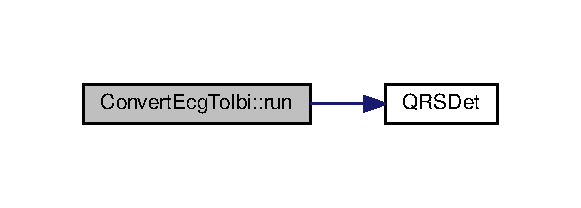
\includegraphics[width=279pt]{classConvertEcgToIbi_a3d9ea57ed19352295382095febc82f71_cgraph}
\end{center}
\end{figure}


\index{Convert\+Ecg\+To\+Ibi@{Convert\+Ecg\+To\+Ibi}!send\+File\+Data@{send\+File\+Data}}
\index{send\+File\+Data@{send\+File\+Data}!Convert\+Ecg\+To\+Ibi@{Convert\+Ecg\+To\+Ibi}}
\subsubsection[{send\+File\+Data}]{\setlength{\rightskip}{0pt plus 5cm}void Convert\+Ecg\+To\+Ibi\+::send\+File\+Data (
\begin{DoxyParamCaption}
\item[{Q\+Vector$<$ double $>$}]{qrs\+Peaks, }
\item[{Q\+Vector$<$ double $>$}]{time\+Data}
\end{DoxyParamCaption}
)\hspace{0.3cm}{\ttfamily [signal]}}\hypertarget{classConvertEcgToIbi_a34d6d61a81e88116c65a2ba9198b7f1c}{}\label{classConvertEcgToIbi_a34d6d61a81e88116c65a2ba9198b7f1c}


send\+File\+Data 


\begin{DoxyParams}{Parameters}
{\em qrs\+Peaks} & Vector containing R-\/R information \\
\hline
{\em time\+Data} & Vector containing time information for the R-\/R data. \\
\hline
\end{DoxyParams}


Here is the caller graph for this function\+:\nopagebreak
\begin{figure}[H]
\begin{center}
\leavevmode
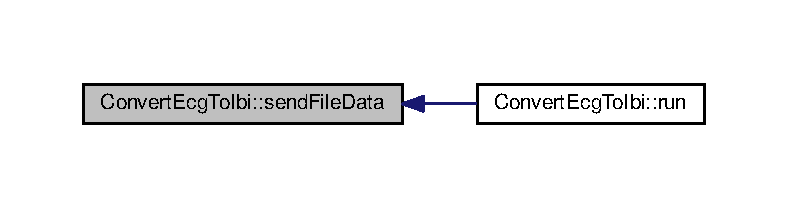
\includegraphics[width=350pt]{classConvertEcgToIbi_a34d6d61a81e88116c65a2ba9198b7f1c_icgraph}
\end{center}
\end{figure}




The documentation for this class was generated from the following files\+:\begin{DoxyCompactItemize}
\item 
src/\hyperlink{convertecgtoibi_8h}{convertecgtoibi.\+h}\item 
src/\hyperlink{convertecgtoibi_8cpp}{convertecgtoibi.\+cpp}\end{DoxyCompactItemize}

\hypertarget{classCurveData}{}\section{Curve\+Data Class Reference}
\label{classCurveData}\index{Curve\+Data@{Curve\+Data}}


Inheritance diagram for Curve\+Data\+:
\nopagebreak
\begin{figure}[H]
\begin{center}
\leavevmode
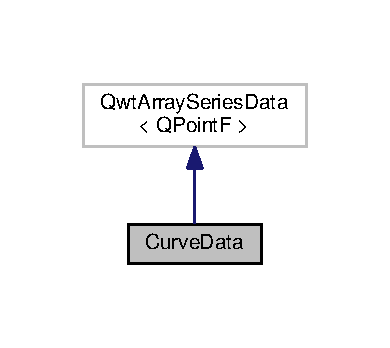
\includegraphics[width=187pt]{classCurveData__inherit__graph}
\end{center}
\end{figure}


Collaboration diagram for Curve\+Data\+:
\nopagebreak
\begin{figure}[H]
\begin{center}
\leavevmode
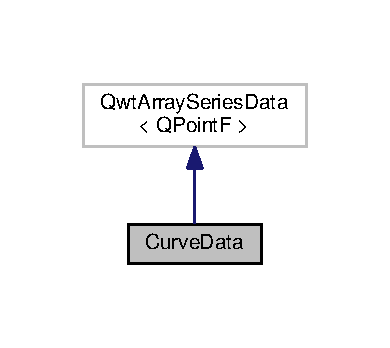
\includegraphics[width=187pt]{classCurveData__coll__graph}
\end{center}
\end{figure}
\subsection*{Public Member Functions}
\begin{DoxyCompactItemize}
\item 
\hyperlink{classCurveData_a4e9a1bb778f0cb2e7d573b88163cfd38}{Curve\+Data} ()
\item 
virtual Q\+RectF \hyperlink{classCurveData_ab915e8d2a5f879804584908a65c5c7f6}{bounding\+Rect} () const 
\item 
void \hyperlink{classCurveData_aff1e348b77d682b9ea65e7724d5679d5}{append} (const Q\+PointF \&point)
\item 
void \hyperlink{classCurveData_ae898810872a274a681ab60131ecf922b}{clear} ()
\end{DoxyCompactItemize}


\subsection{Detailed Description}


Definition at line \hyperlink{plot_8cpp_source_l00013}{13} of file \hyperlink{plot_8cpp_source}{plot.\+cpp}.



\subsection{Constructor \& Destructor Documentation}
\index{Curve\+Data@{Curve\+Data}!Curve\+Data@{Curve\+Data}}
\index{Curve\+Data@{Curve\+Data}!Curve\+Data@{Curve\+Data}}
\subsubsection[{Curve\+Data()}]{\setlength{\rightskip}{0pt plus 5cm}Curve\+Data\+::\+Curve\+Data (
\begin{DoxyParamCaption}
{}
\end{DoxyParamCaption}
)\hspace{0.3cm}{\ttfamily [inline]}}\hypertarget{classCurveData_a4e9a1bb778f0cb2e7d573b88163cfd38}{}\label{classCurveData_a4e9a1bb778f0cb2e7d573b88163cfd38}


Definition at line \hyperlink{plot_8cpp_source_l00016}{16} of file \hyperlink{plot_8cpp_source}{plot.\+cpp}.



\subsection{Member Function Documentation}
\index{Curve\+Data@{Curve\+Data}!append@{append}}
\index{append@{append}!Curve\+Data@{Curve\+Data}}
\subsubsection[{append(const Q\+Point\+F \&point)}]{\setlength{\rightskip}{0pt plus 5cm}void Curve\+Data\+::append (
\begin{DoxyParamCaption}
\item[{const Q\+PointF \&}]{point}
\end{DoxyParamCaption}
)\hspace{0.3cm}{\ttfamily [inline]}}\hypertarget{classCurveData_aff1e348b77d682b9ea65e7724d5679d5}{}\label{classCurveData_aff1e348b77d682b9ea65e7724d5679d5}


Definition at line \hyperlink{plot_8cpp_source_l00028}{28} of file \hyperlink{plot_8cpp_source}{plot.\+cpp}.



Here is the caller graph for this function\+:
\nopagebreak
\begin{figure}[H]
\begin{center}
\leavevmode
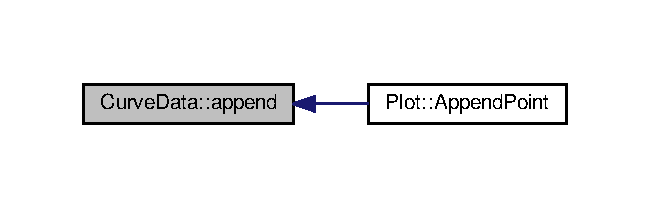
\includegraphics[width=312pt]{classCurveData_aff1e348b77d682b9ea65e7724d5679d5_icgraph}
\end{center}
\end{figure}


\index{Curve\+Data@{Curve\+Data}!bounding\+Rect@{bounding\+Rect}}
\index{bounding\+Rect@{bounding\+Rect}!Curve\+Data@{Curve\+Data}}
\subsubsection[{bounding\+Rect() const }]{\setlength{\rightskip}{0pt plus 5cm}virtual Q\+RectF Curve\+Data\+::bounding\+Rect (
\begin{DoxyParamCaption}
{}
\end{DoxyParamCaption}
) const\hspace{0.3cm}{\ttfamily [inline]}, {\ttfamily [virtual]}}\hypertarget{classCurveData_ab915e8d2a5f879804584908a65c5c7f6}{}\label{classCurveData_ab915e8d2a5f879804584908a65c5c7f6}


Definition at line \hyperlink{plot_8cpp_source_l00020}{20} of file \hyperlink{plot_8cpp_source}{plot.\+cpp}.

\index{Curve\+Data@{Curve\+Data}!clear@{clear}}
\index{clear@{clear}!Curve\+Data@{Curve\+Data}}
\subsubsection[{clear()}]{\setlength{\rightskip}{0pt plus 5cm}void Curve\+Data\+::clear (
\begin{DoxyParamCaption}
{}
\end{DoxyParamCaption}
)\hspace{0.3cm}{\ttfamily [inline]}}\hypertarget{classCurveData_ae898810872a274a681ab60131ecf922b}{}\label{classCurveData_ae898810872a274a681ab60131ecf922b}


Definition at line \hyperlink{plot_8cpp_source_l00033}{33} of file \hyperlink{plot_8cpp_source}{plot.\+cpp}.



Here is the caller graph for this function\+:
\nopagebreak
\begin{figure}[H]
\begin{center}
\leavevmode
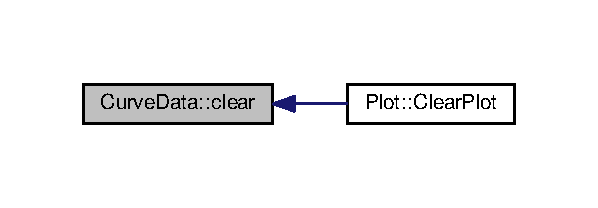
\includegraphics[width=287pt]{classCurveData_ae898810872a274a681ab60131ecf922b_icgraph}
\end{center}
\end{figure}




The documentation for this class was generated from the following file\+:\begin{DoxyCompactItemize}
\item 
src/\hyperlink{plot_8cpp}{plot.\+cpp}\end{DoxyCompactItemize}

\hypertarget{classDataLogger}{}\section{Data\+Logger Class Reference}
\label{classDataLogger}\index{Data\+Logger@{Data\+Logger}}


The \hyperlink{classDataLogger}{Data\+Logger} class.  




{\ttfamily \#include $<$datalogger.\+h$>$}



Inheritance diagram for Data\+Logger\+:\nopagebreak
\begin{figure}[H]
\begin{center}
\leavevmode
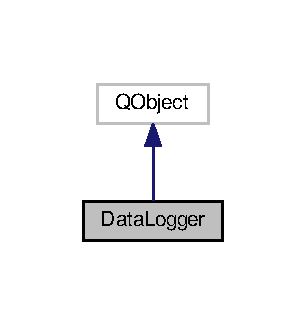
\includegraphics[width=147pt]{classDataLogger__inherit__graph}
\end{center}
\end{figure}


Collaboration diagram for Data\+Logger\+:\nopagebreak
\begin{figure}[H]
\begin{center}
\leavevmode
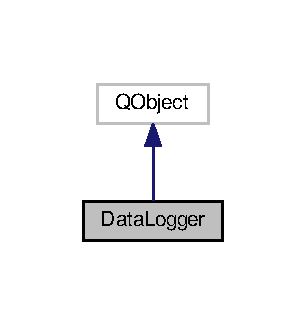
\includegraphics[width=147pt]{classDataLogger__coll__graph}
\end{center}
\end{figure}
\subsection*{Signals}
\begin{DoxyCompactItemize}
\item 
void \hyperlink{classDataLogger_a59e42d6e77f7fd97ea23529abb6c275c}{update\+Status} (Q\+String status)
\begin{DoxyCompactList}\small\item\em Signal emitting status messages during the process. \end{DoxyCompactList}\end{DoxyCompactItemize}
\subsection*{Public Member Functions}
\begin{DoxyCompactItemize}
\item 
\hyperlink{classDataLogger_a4b383913e0fd834ff9b0d8bbd295c2db}{Data\+Logger} (Q\+Object $\ast$parent=0)
\item 
\hyperlink{classDataLogger_a9aaff109f3e7749a0a0a0313655da50a}{$\sim$\+Data\+Logger} ()
\item 
void \hyperlink{classDataLogger_a17296a2d3088e979c9b1f48e68caf9ad}{save} (\hyperlink{classDataStream}{Data\+Stream} \&input)
\begin{DoxyCompactList}\small\item\em Saves the input to a txt-\/file, header-\/file and edf-\/file(if bool save\+As\+Edf in \hyperlink{classSettingsSingleton}{Settings\+Singleton}) \end{DoxyCompactList}\end{DoxyCompactItemize}


\subsection{Detailed Description}
The \hyperlink{classDataLogger}{Data\+Logger} class. 

\begin{DoxyAuthor}{Author}
Martin 
\end{DoxyAuthor}


Definition at line \hyperlink{datalogger_8h_source_l00016}{16} of file \hyperlink{datalogger_8h_source}{datalogger.\+h}.



\subsection{Constructor \& Destructor Documentation}
\index{Data\+Logger@{Data\+Logger}!Data\+Logger@{Data\+Logger}}
\index{Data\+Logger@{Data\+Logger}!Data\+Logger@{Data\+Logger}}
\subsubsection[{Data\+Logger(\+Q\+Object $\ast$parent=0)}]{\setlength{\rightskip}{0pt plus 5cm}Data\+Logger\+::\+Data\+Logger (
\begin{DoxyParamCaption}
\item[{Q\+Object $\ast$}]{parent = {\ttfamily 0}}
\end{DoxyParamCaption}
)\hspace{0.3cm}{\ttfamily [explicit]}}\hypertarget{classDataLogger_a4b383913e0fd834ff9b0d8bbd295c2db}{}\label{classDataLogger_a4b383913e0fd834ff9b0d8bbd295c2db}


Definition at line \hyperlink{datalogger_8cpp_source_l00009}{9} of file \hyperlink{datalogger_8cpp_source}{datalogger.\+cpp}.

\index{Data\+Logger@{Data\+Logger}!````~Data\+Logger@{$\sim$\+Data\+Logger}}
\index{````~Data\+Logger@{$\sim$\+Data\+Logger}!Data\+Logger@{Data\+Logger}}
\subsubsection[{$\sim$\+Data\+Logger()}]{\setlength{\rightskip}{0pt plus 5cm}Data\+Logger\+::$\sim$\+Data\+Logger (
\begin{DoxyParamCaption}
{}
\end{DoxyParamCaption}
)}\hypertarget{classDataLogger_a9aaff109f3e7749a0a0a0313655da50a}{}\label{classDataLogger_a9aaff109f3e7749a0a0a0313655da50a}


Definition at line \hyperlink{datalogger_8cpp_source_l00014}{14} of file \hyperlink{datalogger_8cpp_source}{datalogger.\+cpp}.



\subsection{Member Function Documentation}
\index{Data\+Logger@{Data\+Logger}!save@{save}}
\index{save@{save}!Data\+Logger@{Data\+Logger}}
\subsubsection[{save(\+Data\+Stream \&input)}]{\setlength{\rightskip}{0pt plus 5cm}void Data\+Logger\+::save (
\begin{DoxyParamCaption}
\item[{{\bf Data\+Stream} \&}]{input}
\end{DoxyParamCaption}
)}\hypertarget{classDataLogger_a17296a2d3088e979c9b1f48e68caf9ad}{}\label{classDataLogger_a17296a2d3088e979c9b1f48e68caf9ad}


Saves the input to a txt-\/file, header-\/file and edf-\/file(if bool save\+As\+Edf in \hyperlink{classSettingsSingleton}{Settings\+Singleton}) 

Saves the information from an \hyperlink{structEcgStreamObject}{Ecg\+Stream\+Object} stored in a \hyperlink{classDataStream}{Data\+Stream} vector.

lements. 

Definition at line \hyperlink{datalogger_8cpp_source_l00021}{21} of file \hyperlink{datalogger_8cpp_source}{datalogger.\+cpp}.



Here is the call graph for this function\+:\nopagebreak
\begin{figure}[H]
\begin{center}
\leavevmode
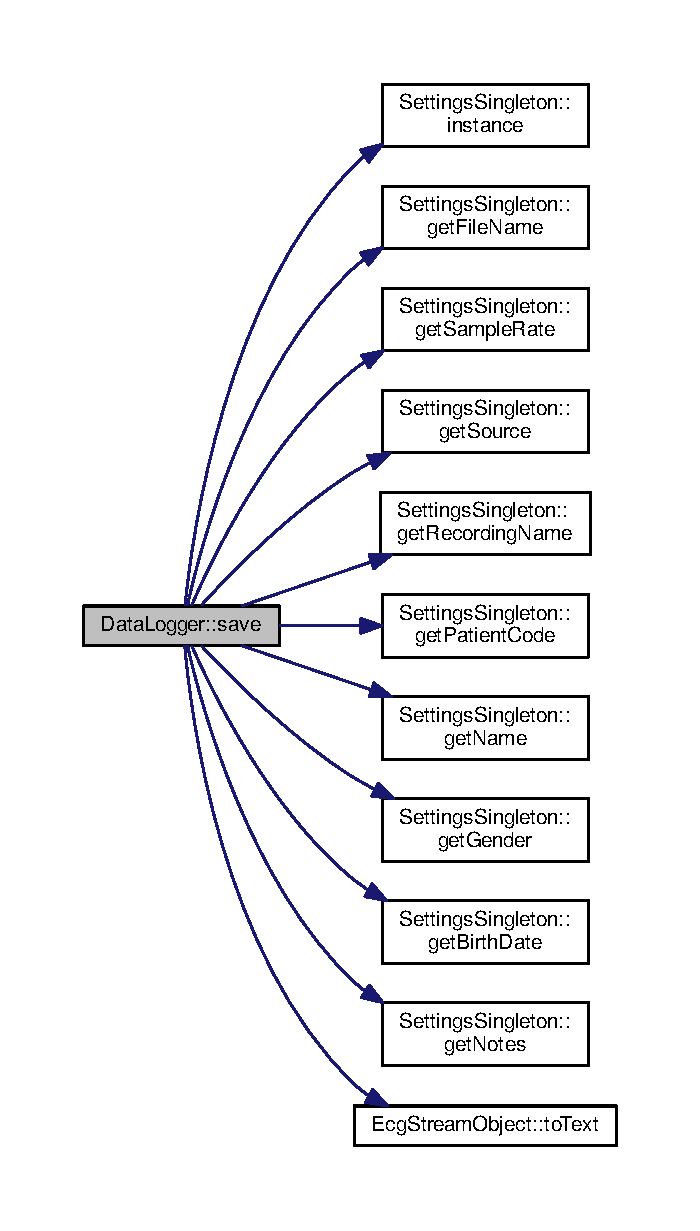
\includegraphics[height=550pt]{classDataLogger_a17296a2d3088e979c9b1f48e68caf9ad_cgraph}
\end{center}
\end{figure}




Here is the caller graph for this function\+:\nopagebreak
\begin{figure}[H]
\begin{center}
\leavevmode
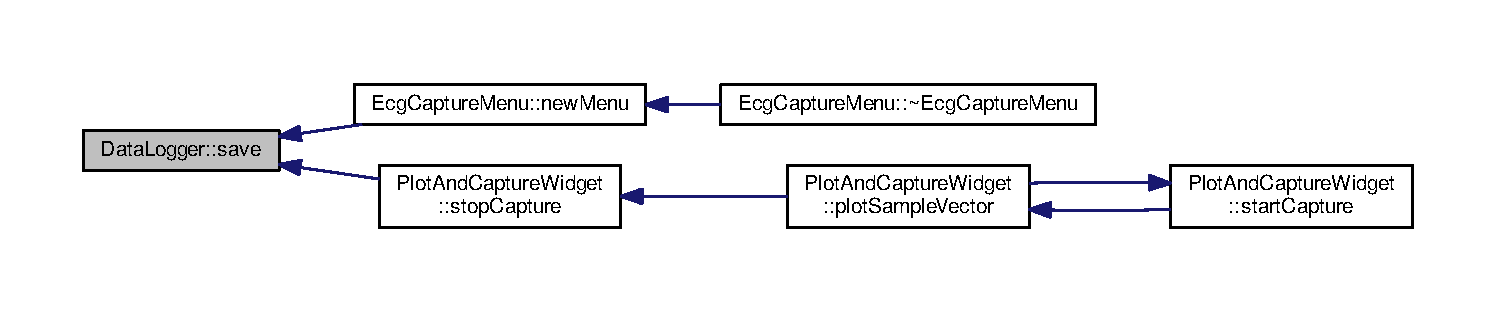
\includegraphics[width=350pt]{classDataLogger_a17296a2d3088e979c9b1f48e68caf9ad_icgraph}
\end{center}
\end{figure}


\index{Data\+Logger@{Data\+Logger}!update\+Status@{update\+Status}}
\index{update\+Status@{update\+Status}!Data\+Logger@{Data\+Logger}}
\subsubsection[{update\+Status}]{\setlength{\rightskip}{0pt plus 5cm}void Data\+Logger\+::update\+Status (
\begin{DoxyParamCaption}
\item[{Q\+String}]{status}
\end{DoxyParamCaption}
)\hspace{0.3cm}{\ttfamily [signal]}}\hypertarget{classDataLogger_a59e42d6e77f7fd97ea23529abb6c275c}{}\label{classDataLogger_a59e42d6e77f7fd97ea23529abb6c275c}


Signal emitting status messages during the process. 



Here is the caller graph for this function\+:\nopagebreak
\begin{figure}[H]
\begin{center}
\leavevmode
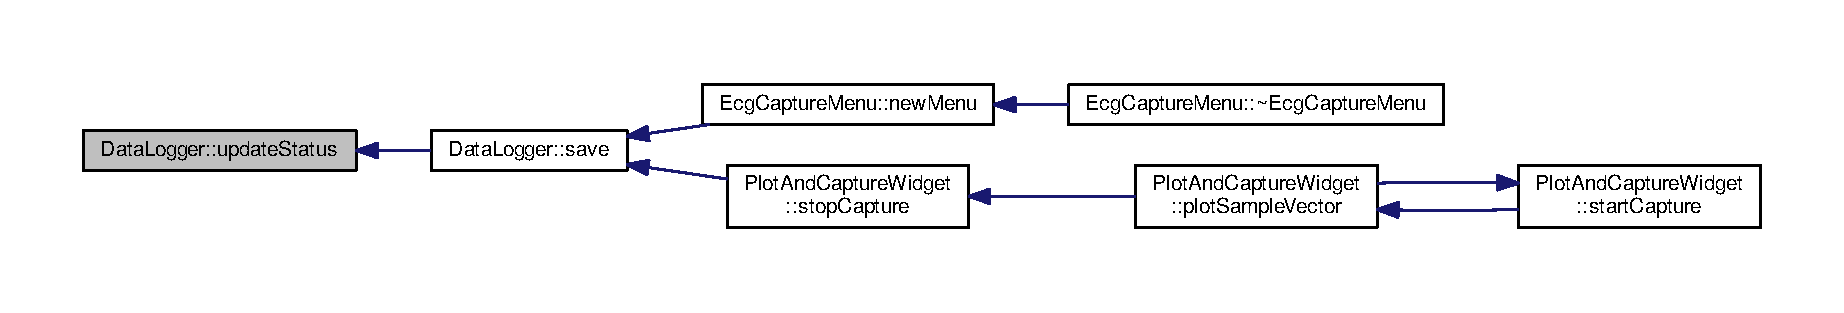
\includegraphics[width=350pt]{classDataLogger_a59e42d6e77f7fd97ea23529abb6c275c_icgraph}
\end{center}
\end{figure}




The documentation for this class was generated from the following files\+:\begin{DoxyCompactItemize}
\item 
src/\hyperlink{datalogger_8h}{datalogger.\+h}\item 
src/\hyperlink{datalogger_8cpp}{datalogger.\+cpp}\end{DoxyCompactItemize}

\hypertarget{classDataStream}{}\section{Data\+Stream Class Reference}
\label{classDataStream}\index{Data\+Stream@{Data\+Stream}}


Abstract Interface that should be used for storing data in the memory.  




{\ttfamily \#include $<$datastream.\+h$>$}



Inheritance diagram for Data\+Stream\+:\nopagebreak
\begin{figure}[H]
\begin{center}
\leavevmode
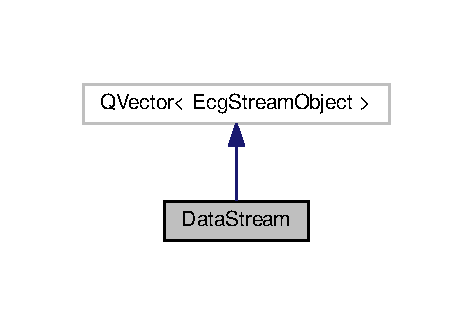
\includegraphics[width=227pt]{classDataStream__inherit__graph}
\end{center}
\end{figure}


Collaboration diagram for Data\+Stream\+:\nopagebreak
\begin{figure}[H]
\begin{center}
\leavevmode
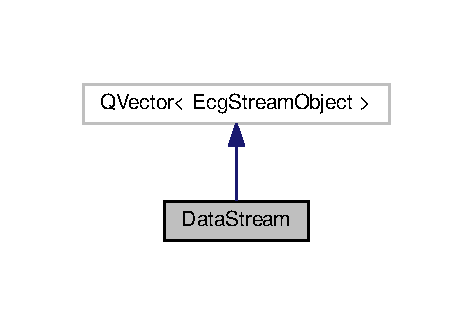
\includegraphics[width=227pt]{classDataStream__coll__graph}
\end{center}
\end{figure}
\subsection*{Public Member Functions}
\begin{DoxyCompactItemize}
\item 
\hyperlink{classDataStream_aadb8f27fe18a349a25b2cd656d686f92}{Data\+Stream} ()
\item 
virtual \hyperlink{classDataStream_ab1ab2421685bd8ee669ec94d3b0239b8}{$\sim$\+Data\+Stream} ()
\item 
Q\+String \hyperlink{classDataStream_a4876a67f0408d22a85ab785a138bcf35}{to\+Text} (int index)
\begin{DoxyCompactList}\small\item\em Text representation of the Object at index. \end{DoxyCompactList}\end{DoxyCompactItemize}
\subsection*{Public Attributes}
\begin{DoxyCompactItemize}
\item 
int \hyperlink{classDataStream_a5b27985e1e797aad7dead2fa690b1638}{sampling\+Rate}
\end{DoxyCompactItemize}


\subsection{Detailed Description}
Abstract Interface that should be used for storing data in the memory. 

\begin{DoxyAuthor}{Author}
Martin 
\end{DoxyAuthor}


Definition at line \hyperlink{datastream_8h_source_l00016}{16} of file \hyperlink{datastream_8h_source}{datastream.\+h}.



\subsection{Constructor \& Destructor Documentation}
\index{Data\+Stream@{Data\+Stream}!Data\+Stream@{Data\+Stream}}
\index{Data\+Stream@{Data\+Stream}!Data\+Stream@{Data\+Stream}}
\subsubsection[{Data\+Stream()}]{\setlength{\rightskip}{0pt plus 5cm}Data\+Stream\+::\+Data\+Stream (
\begin{DoxyParamCaption}
{}
\end{DoxyParamCaption}
)}\hypertarget{classDataStream_aadb8f27fe18a349a25b2cd656d686f92}{}\label{classDataStream_aadb8f27fe18a349a25b2cd656d686f92}


Definition at line \hyperlink{datastream_8cpp_source_l00003}{3} of file \hyperlink{datastream_8cpp_source}{datastream.\+cpp}.

\index{Data\+Stream@{Data\+Stream}!````~Data\+Stream@{$\sim$\+Data\+Stream}}
\index{````~Data\+Stream@{$\sim$\+Data\+Stream}!Data\+Stream@{Data\+Stream}}
\subsubsection[{$\sim$\+Data\+Stream()}]{\setlength{\rightskip}{0pt plus 5cm}Data\+Stream\+::$\sim$\+Data\+Stream (
\begin{DoxyParamCaption}
{}
\end{DoxyParamCaption}
)\hspace{0.3cm}{\ttfamily [virtual]}}\hypertarget{classDataStream_ab1ab2421685bd8ee669ec94d3b0239b8}{}\label{classDataStream_ab1ab2421685bd8ee669ec94d3b0239b8}


Definition at line \hyperlink{datastream_8cpp_source_l00008}{8} of file \hyperlink{datastream_8cpp_source}{datastream.\+cpp}.



\subsection{Member Function Documentation}
\index{Data\+Stream@{Data\+Stream}!to\+Text@{to\+Text}}
\index{to\+Text@{to\+Text}!Data\+Stream@{Data\+Stream}}
\subsubsection[{to\+Text(int index)}]{\setlength{\rightskip}{0pt plus 5cm}Q\+String Data\+Stream\+::to\+Text (
\begin{DoxyParamCaption}
\item[{int}]{index}
\end{DoxyParamCaption}
)}\hypertarget{classDataStream_a4876a67f0408d22a85ab785a138bcf35}{}\label{classDataStream_a4876a67f0408d22a85ab785a138bcf35}


Text representation of the Object at index. 


\begin{DoxyParams}{Parameters}
{\em index} & Index of wanted \hyperlink{structEcgStreamObject}{Ecg\+Stream\+Object} \\
\hline
\end{DoxyParams}
\begin{DoxyReturn}{Returns}
Q\+String contationg the data of the \hyperlink{structEcgStreamObject}{Ecg\+Stream\+Object} 
\end{DoxyReturn}


Definition at line \hyperlink{datastream_8cpp_source_l00013}{13} of file \hyperlink{datastream_8cpp_source}{datastream.\+cpp}.



\subsection{Member Data Documentation}
\index{Data\+Stream@{Data\+Stream}!sampling\+Rate@{sampling\+Rate}}
\index{sampling\+Rate@{sampling\+Rate}!Data\+Stream@{Data\+Stream}}
\subsubsection[{sampling\+Rate}]{\setlength{\rightskip}{0pt plus 5cm}int Data\+Stream\+::sampling\+Rate}\hypertarget{classDataStream_a5b27985e1e797aad7dead2fa690b1638}{}\label{classDataStream_a5b27985e1e797aad7dead2fa690b1638}


Definition at line \hyperlink{datastream_8h_source_l00028}{28} of file \hyperlink{datastream_8h_source}{datastream.\+h}.



The documentation for this class was generated from the following files\+:\begin{DoxyCompactItemize}
\item 
src/\hyperlink{datastream_8h}{datastream.\+h}\item 
src/\hyperlink{datastream_8cpp}{datastream.\+cpp}\end{DoxyCompactItemize}

\hypertarget{classDeviceInterface}{}\section{Device\+Interface Class Reference}
\label{classDeviceInterface}\index{Device\+Interface@{Device\+Interface}}


Abstract interface for all devices.  




{\ttfamily \#include $<$deviceinterface.\+h$>$}



Inheritance diagram for Device\+Interface\+:\nopagebreak
\begin{figure}[H]
\begin{center}
\leavevmode
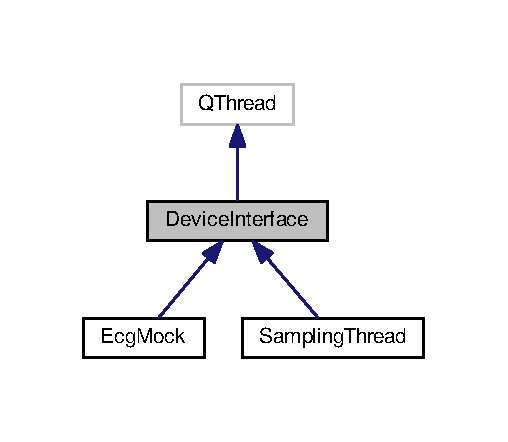
\includegraphics[width=244pt]{classDeviceInterface__inherit__graph}
\end{center}
\end{figure}


Collaboration diagram for Device\+Interface\+:\nopagebreak
\begin{figure}[H]
\begin{center}
\leavevmode
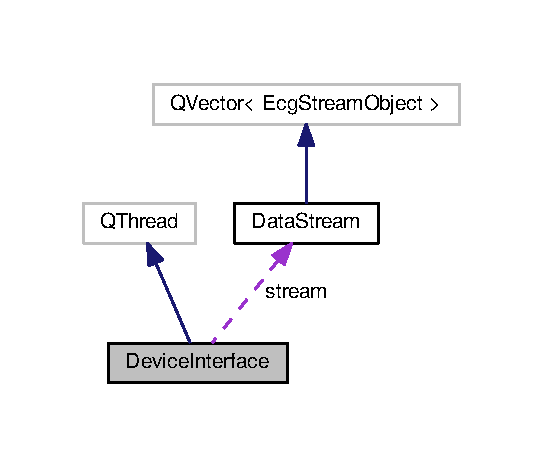
\includegraphics[width=261pt]{classDeviceInterface__coll__graph}
\end{center}
\end{figure}
\subsection*{Signals}
\begin{DoxyCompactItemize}
\item 
void \hyperlink{classDeviceInterface_ae1bcd766865161a659076d2561e79dc5}{send\+Sample\+Vector} (Q\+Vector$<$ Q\+Vector$<$ Q\+PointF $>$ $>$)
\item 
void \hyperlink{classDeviceInterface_ac64a65f54f41f0b7ff4c846ac7fdbef7}{update\+Status} (Q\+String)
\end{DoxyCompactItemize}
\subsection*{Public Member Functions}
\begin{DoxyCompactItemize}
\item 
\hyperlink{classDeviceInterface_a9923935a7fa7b3134568ec7fd97705e3}{Device\+Interface} (\hyperlink{classDataStream}{Data\+Stream} \&input\+Stream)
\item 
virtual \hyperlink{classDeviceInterface_a668a221c7a77701e25719f406d407746}{$\sim$\+Device\+Interface} ()
\item 
virtual void \hyperlink{classDeviceInterface_aeaf032ef412df905fe4f2609cc284887}{get\+Data} (\hyperlink{classDataStream}{Data\+Stream} \&)=0
\item 
virtual bool \hyperlink{classDeviceInterface_a4c7fa83218b6a7c5700cb75253b2165e}{connected} ()=0
\item 
virtual void \hyperlink{classDeviceInterface_a03e9c1bfeabe1a97f05bf9107b89ae67}{init} (\hyperlink{classDataStream}{Data\+Stream} \&)
\item 
virtual void \hyperlink{classDeviceInterface_a08473443413b1725a3930aace12e2837}{close} ()=0
\item 
virtual void \hyperlink{classDeviceInterface_a6511c2845f5198acc94f5d7dd21cae57}{run} ()=0
\item 
virtual void \hyperlink{classDeviceInterface_a101b3b53a01add866737920e03a850a8}{stop} ()=0
\end{DoxyCompactItemize}
\subsection*{Protected Member Functions}
\begin{DoxyCompactItemize}
\item 
void \hyperlink{classDeviceInterface_a83df9dc924dbe0e6c3e0d0fef2a604d0}{update\+Status\+Function} (Q\+String)
\item 
void \hyperlink{classDeviceInterface_adae4c7e07e9bdbbe62be961fd306b5c8}{send\+Sample\+Vector\+Function} (Q\+Vector$<$ Q\+Vector$<$ Q\+PointF $>$ $>$)
\end{DoxyCompactItemize}
\subsection*{Protected Attributes}
\begin{DoxyCompactItemize}
\item 
\hyperlink{classDataStream}{Data\+Stream} \& \hyperlink{classDeviceInterface_ac98f5cd34bafb43265436b29b9f734fa}{stream}
\end{DoxyCompactItemize}


\subsection{Detailed Description}
Abstract interface for all devices. 

Specifies pure virtual functions that specifies the functionality all devices should have

\begin{DoxyAuthor}{Author}
Martin 
\end{DoxyAuthor}


Definition at line \hyperlink{deviceinterface_8h_source_l00029}{29} of file \hyperlink{deviceinterface_8h_source}{deviceinterface.\+h}.



\subsection{Constructor \& Destructor Documentation}
\index{Device\+Interface@{Device\+Interface}!Device\+Interface@{Device\+Interface}}
\index{Device\+Interface@{Device\+Interface}!Device\+Interface@{Device\+Interface}}
\subsubsection[{Device\+Interface(\+Data\+Stream \&input\+Stream)}]{\setlength{\rightskip}{0pt plus 5cm}Device\+Interface\+::\+Device\+Interface (
\begin{DoxyParamCaption}
\item[{{\bf Data\+Stream} \&}]{input\+Stream}
\end{DoxyParamCaption}
)}\hypertarget{classDeviceInterface_a9923935a7fa7b3134568ec7fd97705e3}{}\label{classDeviceInterface_a9923935a7fa7b3134568ec7fd97705e3}


Definition at line \hyperlink{deviceinterface_8cpp_source_l00004}{4} of file \hyperlink{deviceinterface_8cpp_source}{deviceinterface.\+cpp}.

\index{Device\+Interface@{Device\+Interface}!````~Device\+Interface@{$\sim$\+Device\+Interface}}
\index{````~Device\+Interface@{$\sim$\+Device\+Interface}!Device\+Interface@{Device\+Interface}}
\subsubsection[{$\sim$\+Device\+Interface()}]{\setlength{\rightskip}{0pt plus 5cm}Device\+Interface\+::$\sim$\+Device\+Interface (
\begin{DoxyParamCaption}
{}
\end{DoxyParamCaption}
)\hspace{0.3cm}{\ttfamily [virtual]}}\hypertarget{classDeviceInterface_a668a221c7a77701e25719f406d407746}{}\label{classDeviceInterface_a668a221c7a77701e25719f406d407746}


Definition at line \hyperlink{deviceinterface_8cpp_source_l00008}{8} of file \hyperlink{deviceinterface_8cpp_source}{deviceinterface.\+cpp}.



\subsection{Member Function Documentation}
\index{Device\+Interface@{Device\+Interface}!close@{close}}
\index{close@{close}!Device\+Interface@{Device\+Interface}}
\subsubsection[{close()=0}]{\setlength{\rightskip}{0pt plus 5cm}virtual void Device\+Interface\+::close (
\begin{DoxyParamCaption}
{}
\end{DoxyParamCaption}
)\hspace{0.3cm}{\ttfamily [pure virtual]}}\hypertarget{classDeviceInterface_a08473443413b1725a3930aace12e2837}{}\label{classDeviceInterface_a08473443413b1725a3930aace12e2837}


Implemented in \hyperlink{classSamplingThread_aade561b442e580b0ca4af112de2d7a41}{Sampling\+Thread}, and \hyperlink{classEcgMock_a34af13005b5ea44386b7b875b72e9fc3}{Ecg\+Mock}.

\index{Device\+Interface@{Device\+Interface}!connected@{connected}}
\index{connected@{connected}!Device\+Interface@{Device\+Interface}}
\subsubsection[{connected()=0}]{\setlength{\rightskip}{0pt plus 5cm}virtual bool Device\+Interface\+::connected (
\begin{DoxyParamCaption}
{}
\end{DoxyParamCaption}
)\hspace{0.3cm}{\ttfamily [pure virtual]}}\hypertarget{classDeviceInterface_a4c7fa83218b6a7c5700cb75253b2165e}{}\label{classDeviceInterface_a4c7fa83218b6a7c5700cb75253b2165e}


Implemented in \hyperlink{classSamplingThread_a0770f5d1d0c0160cf023fae294010961}{Sampling\+Thread}, and \hyperlink{classEcgMock_ab5e3aac9d92b52b23fafb6e540902f28}{Ecg\+Mock}.

\index{Device\+Interface@{Device\+Interface}!get\+Data@{get\+Data}}
\index{get\+Data@{get\+Data}!Device\+Interface@{Device\+Interface}}
\subsubsection[{get\+Data(\+Data\+Stream \&)=0}]{\setlength{\rightskip}{0pt plus 5cm}virtual void Device\+Interface\+::get\+Data (
\begin{DoxyParamCaption}
\item[{{\bf Data\+Stream} \&}]{}
\end{DoxyParamCaption}
)\hspace{0.3cm}{\ttfamily [pure virtual]}}\hypertarget{classDeviceInterface_aeaf032ef412df905fe4f2609cc284887}{}\label{classDeviceInterface_aeaf032ef412df905fe4f2609cc284887}


Implemented in \hyperlink{classSamplingThread_aa52f1e7171ae5cb8432e949635b02d25}{Sampling\+Thread}, and \hyperlink{classEcgMock_aaa2628c0e8364980e6f252dfc3b86d1a}{Ecg\+Mock}.



Here is the caller graph for this function\+:\nopagebreak
\begin{figure}[H]
\begin{center}
\leavevmode
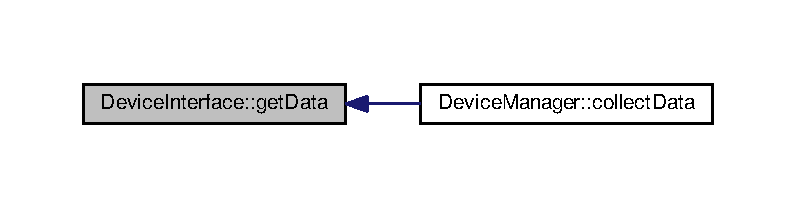
\includegraphics[width=350pt]{classDeviceInterface_aeaf032ef412df905fe4f2609cc284887_icgraph}
\end{center}
\end{figure}


\index{Device\+Interface@{Device\+Interface}!init@{init}}
\index{init@{init}!Device\+Interface@{Device\+Interface}}
\subsubsection[{init(\+Data\+Stream \&)}]{\setlength{\rightskip}{0pt plus 5cm}void Device\+Interface\+::init (
\begin{DoxyParamCaption}
\item[{{\bf Data\+Stream} \&}]{input\+Stream}
\end{DoxyParamCaption}
)\hspace{0.3cm}{\ttfamily [virtual]}}\hypertarget{classDeviceInterface_a03e9c1bfeabe1a97f05bf9107b89ae67}{}\label{classDeviceInterface_a03e9c1bfeabe1a97f05bf9107b89ae67}


Definition at line \hyperlink{deviceinterface_8cpp_source_l00011}{11} of file \hyperlink{deviceinterface_8cpp_source}{deviceinterface.\+cpp}.



Here is the caller graph for this function\+:\nopagebreak
\begin{figure}[H]
\begin{center}
\leavevmode
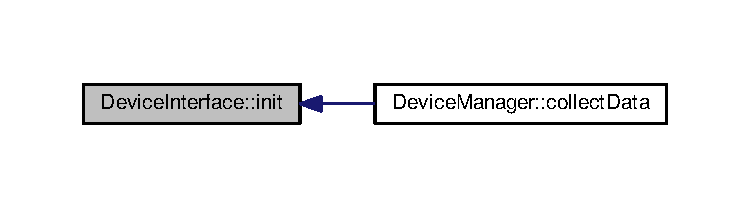
\includegraphics[width=350pt]{classDeviceInterface_a03e9c1bfeabe1a97f05bf9107b89ae67_icgraph}
\end{center}
\end{figure}


\index{Device\+Interface@{Device\+Interface}!run@{run}}
\index{run@{run}!Device\+Interface@{Device\+Interface}}
\subsubsection[{run()=0}]{\setlength{\rightskip}{0pt plus 5cm}virtual void Device\+Interface\+::run (
\begin{DoxyParamCaption}
{}
\end{DoxyParamCaption}
)\hspace{0.3cm}{\ttfamily [pure virtual]}}\hypertarget{classDeviceInterface_a6511c2845f5198acc94f5d7dd21cae57}{}\label{classDeviceInterface_a6511c2845f5198acc94f5d7dd21cae57}


Implemented in \hyperlink{classSamplingThread_a3145c2d8049b3f126f78cb1274154eeb}{Sampling\+Thread}, and \hyperlink{classEcgMock_a8822f99759fcfe9648262007cb380daa}{Ecg\+Mock}.

\index{Device\+Interface@{Device\+Interface}!send\+Sample\+Vector@{send\+Sample\+Vector}}
\index{send\+Sample\+Vector@{send\+Sample\+Vector}!Device\+Interface@{Device\+Interface}}
\subsubsection[{send\+Sample\+Vector}]{\setlength{\rightskip}{0pt plus 5cm}void Device\+Interface\+::send\+Sample\+Vector (
\begin{DoxyParamCaption}
\item[{Q\+Vector$<$ Q\+Vector$<$ Q\+PointF $>$ $>$}]{}
\end{DoxyParamCaption}
)\hspace{0.3cm}{\ttfamily [signal]}}\hypertarget{classDeviceInterface_ae1bcd766865161a659076d2561e79dc5}{}\label{classDeviceInterface_ae1bcd766865161a659076d2561e79dc5}


Here is the caller graph for this function\+:\nopagebreak
\begin{figure}[H]
\begin{center}
\leavevmode
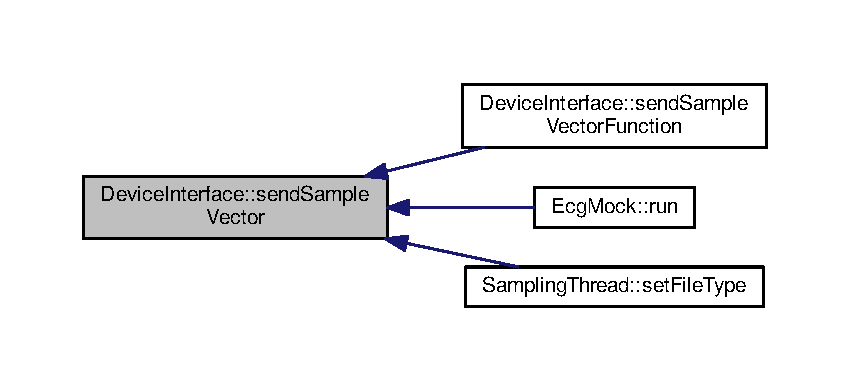
\includegraphics[width=350pt]{classDeviceInterface_ae1bcd766865161a659076d2561e79dc5_icgraph}
\end{center}
\end{figure}


\index{Device\+Interface@{Device\+Interface}!send\+Sample\+Vector\+Function@{send\+Sample\+Vector\+Function}}
\index{send\+Sample\+Vector\+Function@{send\+Sample\+Vector\+Function}!Device\+Interface@{Device\+Interface}}
\subsubsection[{send\+Sample\+Vector\+Function(\+Q\+Vector$<$ Q\+Vector$<$ Q\+Point\+F $>$ $>$)}]{\setlength{\rightskip}{0pt plus 5cm}void Device\+Interface\+::send\+Sample\+Vector\+Function (
\begin{DoxyParamCaption}
\item[{Q\+Vector$<$ Q\+Vector$<$ Q\+PointF $>$ $>$}]{input}
\end{DoxyParamCaption}
)\hspace{0.3cm}{\ttfamily [protected]}}\hypertarget{classDeviceInterface_adae4c7e07e9bdbbe62be961fd306b5c8}{}\label{classDeviceInterface_adae4c7e07e9bdbbe62be961fd306b5c8}


Definition at line \hyperlink{deviceinterface_8cpp_source_l00014}{14} of file \hyperlink{deviceinterface_8cpp_source}{deviceinterface.\+cpp}.

\index{Device\+Interface@{Device\+Interface}!stop@{stop}}
\index{stop@{stop}!Device\+Interface@{Device\+Interface}}
\subsubsection[{stop()=0}]{\setlength{\rightskip}{0pt plus 5cm}virtual void Device\+Interface\+::stop (
\begin{DoxyParamCaption}
{}
\end{DoxyParamCaption}
)\hspace{0.3cm}{\ttfamily [pure virtual]}}\hypertarget{classDeviceInterface_a101b3b53a01add866737920e03a850a8}{}\label{classDeviceInterface_a101b3b53a01add866737920e03a850a8}


Implemented in \hyperlink{classSamplingThread_a6e758c7b8266755c201ca002520f5e2e}{Sampling\+Thread}, and \hyperlink{classEcgMock_aa65eb7c062913402c77ed1dc628168a7}{Ecg\+Mock}.



Here is the caller graph for this function\+:\nopagebreak
\begin{figure}[H]
\begin{center}
\leavevmode
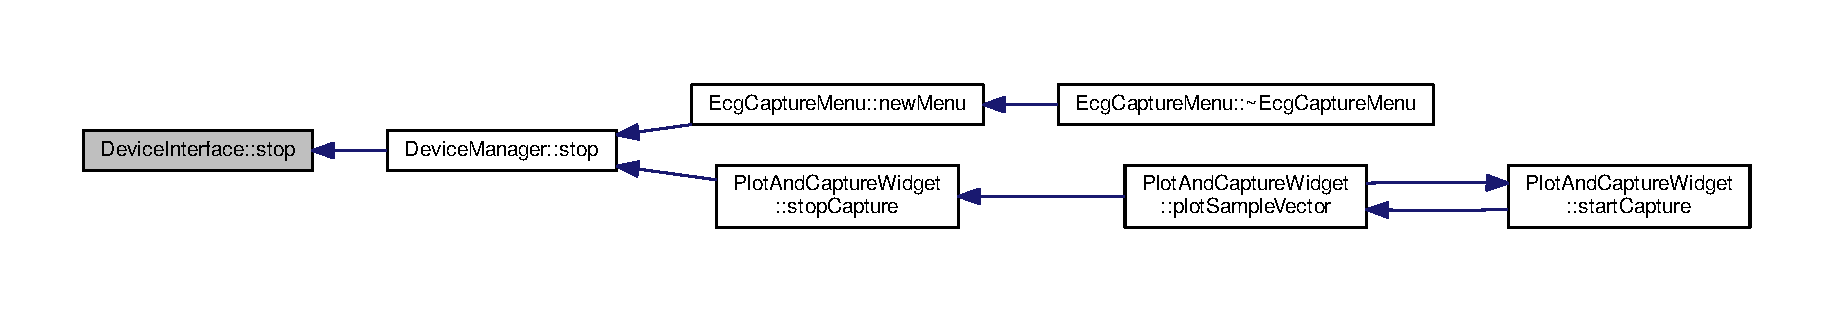
\includegraphics[width=350pt]{classDeviceInterface_a101b3b53a01add866737920e03a850a8_icgraph}
\end{center}
\end{figure}


\index{Device\+Interface@{Device\+Interface}!update\+Status@{update\+Status}}
\index{update\+Status@{update\+Status}!Device\+Interface@{Device\+Interface}}
\subsubsection[{update\+Status}]{\setlength{\rightskip}{0pt plus 5cm}void Device\+Interface\+::update\+Status (
\begin{DoxyParamCaption}
\item[{Q\+String}]{}
\end{DoxyParamCaption}
)\hspace{0.3cm}{\ttfamily [signal]}}\hypertarget{classDeviceInterface_ac64a65f54f41f0b7ff4c846ac7fdbef7}{}\label{classDeviceInterface_ac64a65f54f41f0b7ff4c846ac7fdbef7}


Here is the caller graph for this function\+:\nopagebreak
\begin{figure}[H]
\begin{center}
\leavevmode
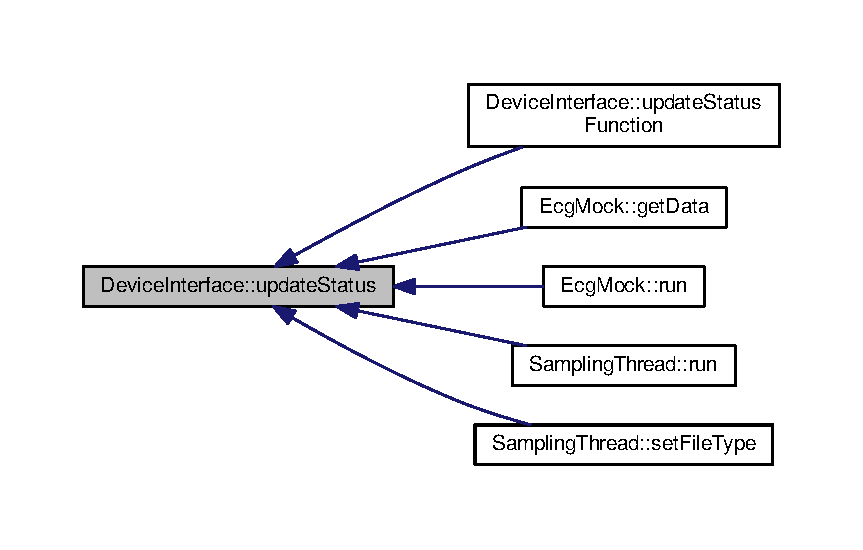
\includegraphics[width=350pt]{classDeviceInterface_ac64a65f54f41f0b7ff4c846ac7fdbef7_icgraph}
\end{center}
\end{figure}


\index{Device\+Interface@{Device\+Interface}!update\+Status\+Function@{update\+Status\+Function}}
\index{update\+Status\+Function@{update\+Status\+Function}!Device\+Interface@{Device\+Interface}}
\subsubsection[{update\+Status\+Function(\+Q\+String)}]{\setlength{\rightskip}{0pt plus 5cm}void Device\+Interface\+::update\+Status\+Function (
\begin{DoxyParamCaption}
\item[{Q\+String}]{input}
\end{DoxyParamCaption}
)\hspace{0.3cm}{\ttfamily [protected]}}\hypertarget{classDeviceInterface_a83df9dc924dbe0e6c3e0d0fef2a604d0}{}\label{classDeviceInterface_a83df9dc924dbe0e6c3e0d0fef2a604d0}


Definition at line \hyperlink{deviceinterface_8cpp_source_l00018}{18} of file \hyperlink{deviceinterface_8cpp_source}{deviceinterface.\+cpp}.



\subsection{Member Data Documentation}
\index{Device\+Interface@{Device\+Interface}!stream@{stream}}
\index{stream@{stream}!Device\+Interface@{Device\+Interface}}
\subsubsection[{stream}]{\setlength{\rightskip}{0pt plus 5cm}{\bf Data\+Stream}\& Device\+Interface\+::stream\hspace{0.3cm}{\ttfamily [protected]}}\hypertarget{classDeviceInterface_ac98f5cd34bafb43265436b29b9f734fa}{}\label{classDeviceInterface_ac98f5cd34bafb43265436b29b9f734fa}


Definition at line \hyperlink{deviceinterface_8h_source_l00048}{48} of file \hyperlink{deviceinterface_8h_source}{deviceinterface.\+h}.



The documentation for this class was generated from the following files\+:\begin{DoxyCompactItemize}
\item 
src/\hyperlink{deviceinterface_8h}{deviceinterface.\+h}\item 
src/\hyperlink{deviceinterface_8cpp}{deviceinterface.\+cpp}\end{DoxyCompactItemize}

\hypertarget{classDeviceManager}{}\section{Device\+Manager Class Reference}
\label{classDeviceManager}\index{Device\+Manager@{Device\+Manager}}


Handles which device to connect through the \hyperlink{classDeviceInterface}{Device\+Interface}.  




{\ttfamily \#include $<$devicemanager.\+h$>$}



Inheritance diagram for Device\+Manager\+:
\nopagebreak
\begin{figure}[H]
\begin{center}
\leavevmode
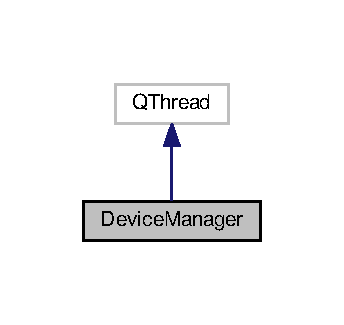
\includegraphics[width=165pt]{classDeviceManager__inherit__graph}
\end{center}
\end{figure}


Collaboration diagram for Device\+Manager\+:
\nopagebreak
\begin{figure}[H]
\begin{center}
\leavevmode
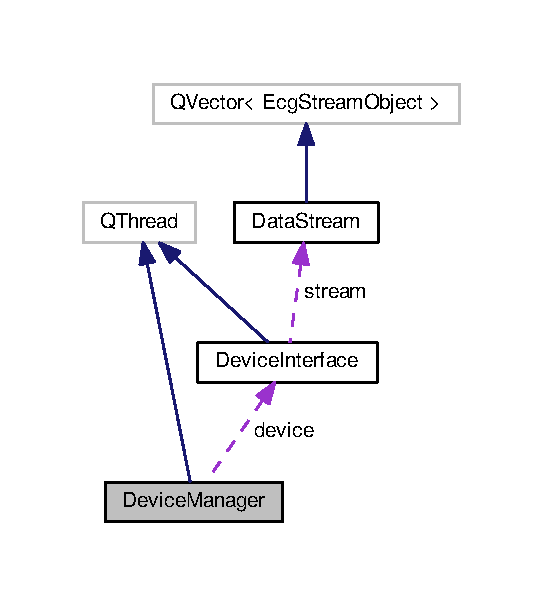
\includegraphics[width=261pt]{classDeviceManager__coll__graph}
\end{center}
\end{figure}
\subsection*{Public Slots}
\begin{DoxyCompactItemize}
\item 
void \hyperlink{classDeviceManager_a14f86d572f6ea7222032ec00499a16a8}{receive\+Sample\+Vector} (Q\+Vector$<$ Q\+Vector$<$ Q\+PointF $>$ $>$)
\begin{DoxyCompactList}\small\item\em Slot used to transfer send\+Sample\+Vector from initiated device to the local signal. \end{DoxyCompactList}\item 
void \hyperlink{classDeviceManager_aa7b96de52a17b961688e81f5e999da74}{receive\+Status} (Q\+String)
\begin{DoxyCompactList}\small\item\em Slot used to transfer update\+Status from initiated device to the local signal. \end{DoxyCompactList}\end{DoxyCompactItemize}
\subsection*{Signals}
\begin{DoxyCompactItemize}
\item 
void \hyperlink{classDeviceManager_a7f0794801ee0b28c74a253f3c2cf5659}{send\+Sample\+Vector} (Q\+Vector$<$ Q\+Vector$<$ Q\+PointF $>$ $>$)
\begin{DoxyCompactList}\small\item\em Sends a Q\+Vector that can be used for a G\+UI to plot in \char`\"{}\+Real-\/time\char`\"{}. \end{DoxyCompactList}\item 
void \hyperlink{classDeviceManager_a68b6e3b924cacf0a5cde44d02eb49d0c}{update\+Status} (Q\+String)
\begin{DoxyCompactList}\small\item\em Information signal for updating status about progress. \end{DoxyCompactList}\end{DoxyCompactItemize}
\subsection*{Public Member Functions}
\begin{DoxyCompactItemize}
\item 
\hyperlink{classDeviceManager_a4e6d37b581df235b46c5696e6c71ae79}{Device\+Manager} ()
\item 
\hyperlink{classDeviceManager_ad91a247c8acfd51c533be52313ce7ddd}{$\sim$\+Device\+Manager} ()
\item 
void \hyperlink{classDeviceManager_a322e3bd6b6f57692116b6af7b9a57a9a}{collect\+Data} (\hyperlink{classDataStream}{Data\+Stream} \&)
\begin{DoxyCompactList}\small\item\em Collects data from the connected device. \end{DoxyCompactList}\item 
void \hyperlink{classDeviceManager_a30358705658f1037ef6bb98e7a2d5e80}{start\+Capture} ()
\begin{DoxyCompactList}\small\item\em Starts the initiated device through a call to start() \end{DoxyCompactList}\item 
void \hyperlink{classDeviceManager_a8569742b2eb08d95052506e372b6bd31}{stop} ()
\begin{DoxyCompactList}\small\item\em Stops the running device. \end{DoxyCompactList}\item 
void \hyperlink{classDeviceManager_a280116304655de3a0bbfbf49730f9384}{init} (int, \hyperlink{classDataStream}{Data\+Stream} \&)
\begin{DoxyCompactList}\small\item\em Prepares a new data-\/collection,. \end{DoxyCompactList}\end{DoxyCompactItemize}
\subsection*{Public Attributes}
\begin{DoxyCompactItemize}
\item 
\hyperlink{classDeviceInterface}{Device\+Interface} $\ast$ \hyperlink{classDeviceManager_aa916ac4224ab9a874e6242c0a9f50a56}{device}
\begin{DoxyCompactList}\small\item\em The connected device. \end{DoxyCompactList}\end{DoxyCompactItemize}


\subsection{Detailed Description}
Handles which device to connect through the \hyperlink{classDeviceInterface}{Device\+Interface}. 

\begin{DoxyAuthor}{Author}
Martin 
\end{DoxyAuthor}


Definition at line \hyperlink{devicemanager_8h_source_l00023}{23} of file \hyperlink{devicemanager_8h_source}{devicemanager.\+h}.



\subsection{Constructor \& Destructor Documentation}
\index{Device\+Manager@{Device\+Manager}!Device\+Manager@{Device\+Manager}}
\index{Device\+Manager@{Device\+Manager}!Device\+Manager@{Device\+Manager}}
\subsubsection[{Device\+Manager()}]{\setlength{\rightskip}{0pt plus 5cm}Device\+Manager\+::\+Device\+Manager (
\begin{DoxyParamCaption}
{}
\end{DoxyParamCaption}
)}\hypertarget{classDeviceManager_a4e6d37b581df235b46c5696e6c71ae79}{}\label{classDeviceManager_a4e6d37b581df235b46c5696e6c71ae79}


Definition at line \hyperlink{devicemanager_8cpp_source_l00010}{10} of file \hyperlink{devicemanager_8cpp_source}{devicemanager.\+cpp}.

\index{Device\+Manager@{Device\+Manager}!````~Device\+Manager@{$\sim$\+Device\+Manager}}
\index{````~Device\+Manager@{$\sim$\+Device\+Manager}!Device\+Manager@{Device\+Manager}}
\subsubsection[{$\sim$\+Device\+Manager()}]{\setlength{\rightskip}{0pt plus 5cm}Device\+Manager\+::$\sim$\+Device\+Manager (
\begin{DoxyParamCaption}
{}
\end{DoxyParamCaption}
)}\hypertarget{classDeviceManager_ad91a247c8acfd51c533be52313ce7ddd}{}\label{classDeviceManager_ad91a247c8acfd51c533be52313ce7ddd}


Definition at line \hyperlink{devicemanager_8cpp_source_l00016}{16} of file \hyperlink{devicemanager_8cpp_source}{devicemanager.\+cpp}.



\subsection{Member Function Documentation}
\index{Device\+Manager@{Device\+Manager}!collect\+Data@{collect\+Data}}
\index{collect\+Data@{collect\+Data}!Device\+Manager@{Device\+Manager}}
\subsubsection[{collect\+Data(\+Data\+Stream \&)}]{\setlength{\rightskip}{0pt plus 5cm}void Device\+Manager\+::collect\+Data (
\begin{DoxyParamCaption}
\item[{{\bf Data\+Stream} \&}]{stream}
\end{DoxyParamCaption}
)}\hypertarget{classDeviceManager_a322e3bd6b6f57692116b6af7b9a57a9a}{}\label{classDeviceManager_a322e3bd6b6f57692116b6af7b9a57a9a}


Collects data from the connected device. 

\begin{DoxyRefDesc}{Deprecated}
\item[\hyperlink{deprecated__deprecated000001}{Deprecated}]\end{DoxyRefDesc}


Definition at line \hyperlink{devicemanager_8cpp_source_l00033}{33} of file \hyperlink{devicemanager_8cpp_source}{devicemanager.\+cpp}.



Here is the call graph for this function\+:
\nopagebreak
\begin{figure}[H]
\begin{center}
\leavevmode
\includegraphics[width=350pt]{classDeviceManager_a322e3bd6b6f57692116b6af7b9a57a9a_cgraph}
\end{center}
\end{figure}


\index{Device\+Manager@{Device\+Manager}!init@{init}}
\index{init@{init}!Device\+Manager@{Device\+Manager}}
\subsubsection[{init(int, Data\+Stream \&)}]{\setlength{\rightskip}{0pt plus 5cm}void Device\+Manager\+::init (
\begin{DoxyParamCaption}
\item[{int}]{device\+Number, }
\item[{{\bf Data\+Stream} \&}]{input\+Stream}
\end{DoxyParamCaption}
)}\hypertarget{classDeviceManager_a280116304655de3a0bbfbf49730f9384}{}\label{classDeviceManager_a280116304655de3a0bbfbf49730f9384}


Prepares a new data-\/collection,. 


\begin{DoxyParams}{Parameters}
{\em device\+Number} & Which device to connect \\
\hline
{\em output\+Stream} & \hyperlink{classDataStream}{Data\+Stream} to store the collected values in. \\
\hline
\end{DoxyParams}


Definition at line \hyperlink{devicemanager_8cpp_source_l00053}{53} of file \hyperlink{devicemanager_8cpp_source}{devicemanager.\+cpp}.



Here is the call graph for this function\+:
\nopagebreak
\begin{figure}[H]
\begin{center}
\leavevmode
\includegraphics[width=350pt]{classDeviceManager_a280116304655de3a0bbfbf49730f9384_cgraph}
\end{center}
\end{figure}




Here is the caller graph for this function\+:
\nopagebreak
\begin{figure}[H]
\begin{center}
\leavevmode
\includegraphics[width=350pt]{classDeviceManager_a280116304655de3a0bbfbf49730f9384_icgraph}
\end{center}
\end{figure}


\index{Device\+Manager@{Device\+Manager}!receive\+Sample\+Vector@{receive\+Sample\+Vector}}
\index{receive\+Sample\+Vector@{receive\+Sample\+Vector}!Device\+Manager@{Device\+Manager}}
\subsubsection[{receive\+Sample\+Vector}]{\setlength{\rightskip}{0pt plus 5cm}void Device\+Manager\+::receive\+Sample\+Vector (
\begin{DoxyParamCaption}
\item[{Q\+Vector$<$ Q\+Vector$<$ Q\+PointF $>$ $>$}]{input}
\end{DoxyParamCaption}
)\hspace{0.3cm}{\ttfamily [slot]}}\hypertarget{classDeviceManager_a14f86d572f6ea7222032ec00499a16a8}{}\label{classDeviceManager_a14f86d572f6ea7222032ec00499a16a8}


Slot used to transfer send\+Sample\+Vector from initiated device to the local signal. 



Definition at line \hyperlink{devicemanager_8cpp_source_l00025}{25} of file \hyperlink{devicemanager_8cpp_source}{devicemanager.\+cpp}.



Here is the caller graph for this function\+:
\nopagebreak
\begin{figure}[H]
\begin{center}
\leavevmode
\includegraphics[width=350pt]{classDeviceManager_a14f86d572f6ea7222032ec00499a16a8_icgraph}
\end{center}
\end{figure}


\index{Device\+Manager@{Device\+Manager}!receive\+Status@{receive\+Status}}
\index{receive\+Status@{receive\+Status}!Device\+Manager@{Device\+Manager}}
\subsubsection[{receive\+Status}]{\setlength{\rightskip}{0pt plus 5cm}void Device\+Manager\+::receive\+Status (
\begin{DoxyParamCaption}
\item[{Q\+String}]{input}
\end{DoxyParamCaption}
)\hspace{0.3cm}{\ttfamily [slot]}}\hypertarget{classDeviceManager_aa7b96de52a17b961688e81f5e999da74}{}\label{classDeviceManager_aa7b96de52a17b961688e81f5e999da74}


Slot used to transfer update\+Status from initiated device to the local signal. 



Definition at line \hyperlink{devicemanager_8cpp_source_l00029}{29} of file \hyperlink{devicemanager_8cpp_source}{devicemanager.\+cpp}.



Here is the caller graph for this function\+:
\nopagebreak
\begin{figure}[H]
\begin{center}
\leavevmode
\includegraphics[width=350pt]{classDeviceManager_aa7b96de52a17b961688e81f5e999da74_icgraph}
\end{center}
\end{figure}


\index{Device\+Manager@{Device\+Manager}!send\+Sample\+Vector@{send\+Sample\+Vector}}
\index{send\+Sample\+Vector@{send\+Sample\+Vector}!Device\+Manager@{Device\+Manager}}
\subsubsection[{send\+Sample\+Vector}]{\setlength{\rightskip}{0pt plus 5cm}void Device\+Manager\+::send\+Sample\+Vector (
\begin{DoxyParamCaption}
\item[{Q\+Vector$<$ Q\+Vector$<$ Q\+PointF $>$ $>$}]{}
\end{DoxyParamCaption}
)\hspace{0.3cm}{\ttfamily [signal]}}\hypertarget{classDeviceManager_a7f0794801ee0b28c74a253f3c2cf5659}{}\label{classDeviceManager_a7f0794801ee0b28c74a253f3c2cf5659}


Sends a Q\+Vector that can be used for a G\+UI to plot in \char`\"{}\+Real-\/time\char`\"{}. 



Here is the caller graph for this function\+:
\nopagebreak
\begin{figure}[H]
\begin{center}
\leavevmode
\includegraphics[width=350pt]{classDeviceManager_a7f0794801ee0b28c74a253f3c2cf5659_icgraph}
\end{center}
\end{figure}


\index{Device\+Manager@{Device\+Manager}!start\+Capture@{start\+Capture}}
\index{start\+Capture@{start\+Capture}!Device\+Manager@{Device\+Manager}}
\subsubsection[{start\+Capture()}]{\setlength{\rightskip}{0pt plus 5cm}void Device\+Manager\+::start\+Capture (
\begin{DoxyParamCaption}
{}
\end{DoxyParamCaption}
)}\hypertarget{classDeviceManager_a30358705658f1037ef6bb98e7a2d5e80}{}\label{classDeviceManager_a30358705658f1037ef6bb98e7a2d5e80}


Starts the initiated device through a call to start() 



Definition at line \hyperlink{devicemanager_8cpp_source_l00042}{42} of file \hyperlink{devicemanager_8cpp_source}{devicemanager.\+cpp}.



Here is the caller graph for this function\+:
\nopagebreak
\begin{figure}[H]
\begin{center}
\leavevmode
\includegraphics[width=350pt]{classDeviceManager_a30358705658f1037ef6bb98e7a2d5e80_icgraph}
\end{center}
\end{figure}


\index{Device\+Manager@{Device\+Manager}!stop@{stop}}
\index{stop@{stop}!Device\+Manager@{Device\+Manager}}
\subsubsection[{stop()}]{\setlength{\rightskip}{0pt plus 5cm}void Device\+Manager\+::stop (
\begin{DoxyParamCaption}
{}
\end{DoxyParamCaption}
)}\hypertarget{classDeviceManager_a8569742b2eb08d95052506e372b6bd31}{}\label{classDeviceManager_a8569742b2eb08d95052506e372b6bd31}


Stops the running device. 

\begin{DoxyRefDesc}{Todo}
\item[\hyperlink{todo__todo000009}{Todo}]use connected() before execution \end{DoxyRefDesc}


Definition at line \hyperlink{devicemanager_8cpp_source_l00049}{49} of file \hyperlink{devicemanager_8cpp_source}{devicemanager.\+cpp}.



Here is the call graph for this function\+:
\nopagebreak
\begin{figure}[H]
\begin{center}
\leavevmode
\includegraphics[width=336pt]{classDeviceManager_a8569742b2eb08d95052506e372b6bd31_cgraph}
\end{center}
\end{figure}




Here is the caller graph for this function\+:
\nopagebreak
\begin{figure}[H]
\begin{center}
\leavevmode
\includegraphics[width=350pt]{classDeviceManager_a8569742b2eb08d95052506e372b6bd31_icgraph}
\end{center}
\end{figure}


\index{Device\+Manager@{Device\+Manager}!update\+Status@{update\+Status}}
\index{update\+Status@{update\+Status}!Device\+Manager@{Device\+Manager}}
\subsubsection[{update\+Status}]{\setlength{\rightskip}{0pt plus 5cm}void Device\+Manager\+::update\+Status (
\begin{DoxyParamCaption}
\item[{Q\+String}]{}
\end{DoxyParamCaption}
)\hspace{0.3cm}{\ttfamily [signal]}}\hypertarget{classDeviceManager_a68b6e3b924cacf0a5cde44d02eb49d0c}{}\label{classDeviceManager_a68b6e3b924cacf0a5cde44d02eb49d0c}


Information signal for updating status about progress. 



Here is the caller graph for this function\+:
\nopagebreak
\begin{figure}[H]
\begin{center}
\leavevmode
\includegraphics[width=350pt]{classDeviceManager_a68b6e3b924cacf0a5cde44d02eb49d0c_icgraph}
\end{center}
\end{figure}




\subsection{Member Data Documentation}
\index{Device\+Manager@{Device\+Manager}!device@{device}}
\index{device@{device}!Device\+Manager@{Device\+Manager}}
\subsubsection[{device}]{\setlength{\rightskip}{0pt plus 5cm}{\bf Device\+Interface}$\ast$ Device\+Manager\+::device}\hypertarget{classDeviceManager_aa916ac4224ab9a874e6242c0a9f50a56}{}\label{classDeviceManager_aa916ac4224ab9a874e6242c0a9f50a56}


The connected device. 



Definition at line \hyperlink{devicemanager_8h_source_l00033}{33} of file \hyperlink{devicemanager_8h_source}{devicemanager.\+h}.



The documentation for this class was generated from the following files\+:\begin{DoxyCompactItemize}
\item 
src/\hyperlink{devicemanager_8h}{devicemanager.\+h}\item 
src/\hyperlink{devicemanager_8cpp}{devicemanager.\+cpp}\end{DoxyCompactItemize}

\hypertarget{classEcgCapture}{}\section{Ecg\+Capture Class Reference}
\label{classEcgCapture}\index{Ecg\+Capture@{Ecg\+Capture}}


Responsible for communication with A\+D\+AS.  




{\ttfamily \#include $<$ecgcapture.\+h$>$}



Inheritance diagram for Ecg\+Capture\+:
\nopagebreak
\begin{figure}[H]
\begin{center}
\leavevmode
\includegraphics[width=148pt]{classEcgCapture__inherit__graph}
\end{center}
\end{figure}


Collaboration diagram for Ecg\+Capture\+:
\nopagebreak
\begin{figure}[H]
\begin{center}
\leavevmode
\includegraphics[width=148pt]{classEcgCapture__coll__graph}
\end{center}
\end{figure}
\subsection*{Public Types}
\begin{DoxyCompactItemize}
\item 
enum \hyperlink{group__Device-Facade_gabf6e5cc9109a573e29add762dc36df9b}{Operating\+Mode} \{ \hyperlink{group__Device-Facade_ggabf6e5cc9109a573e29add762dc36df9ba9e4c8f425af52209ee3eb7c466852b22}{ecg\+Capture}, 
\hyperlink{group__Device-Facade_ggabf6e5cc9109a573e29add762dc36df9ba8b349f0786d8e8247f4bc381baa51134}{test\+Tone\+Square}, 
\hyperlink{group__Device-Facade_ggabf6e5cc9109a573e29add762dc36df9ba9ececd6d5264a0e5996556c6697a4f94}{test\+Tone\+Low\+Freq\+Sin}, 
\hyperlink{group__Device-Facade_ggabf6e5cc9109a573e29add762dc36df9ba397d60b89ddb5aaf41d92c617868ed47}{test\+Tone\+High\+Freq\+Sin}
 \}
\item 
enum \hyperlink{group__Device-Facade_gaaf4f7677ca26944edc0f65195b8729f3}{Frequency} \{ \hyperlink{group__Device-Facade_ggaaf4f7677ca26944edc0f65195b8729f3acb281025a93800e7ed188605a7375838}{low\+Freq}, 
\hyperlink{group__Device-Facade_ggaaf4f7677ca26944edc0f65195b8729f3a2a968734e734a271ef5a52b83360122a}{mid\+Freq}, 
\hyperlink{group__Device-Facade_ggaaf4f7677ca26944edc0f65195b8729f3abd09d184c2c34f227532a8bc5fb90877}{high\+Freq}
 \}
\item 
enum \hyperlink{group__Device-Facade_ga1750ac59389b67ba4d9d2834dd7c2d9c}{lead\+Format} \{ \hyperlink{group__Device-Facade_gga1750ac59389b67ba4d9d2834dd7c2d9caf7786dce131009aa61ddfed4f8d8639b}{digital}, 
\hyperlink{group__Device-Facade_gga1750ac59389b67ba4d9d2834dd7c2d9ca21cabce4f74afcf79d24897058fdd6b9}{electrode}
 \}
\end{DoxyCompactItemize}
\subsection*{Public Member Functions}
\begin{DoxyCompactItemize}
\item 
\hyperlink{group__Device-Facade_gaeef1c0708b94ee82330d6d165a2b5a71}{Ecg\+Capture} ()
\item 
void \hyperlink{group__Device-Facade_ga8f080b59e8caab0993bb7ee6b872b6a0}{init} (\hyperlink{group__Device-Facade_gabf6e5cc9109a573e29add762dc36df9b}{Operating\+Mode}, \hyperlink{group__Device-Facade_gaaf4f7677ca26944edc0f65195b8729f3}{Frequency})
\begin{DoxyCompactList}\small\item\em Initiate the device by configuring the registers depending on operating mode and sampling frequency. \end{DoxyCompactList}\item 
void \hyperlink{group__Device-Facade_ga9582047c81db34a3cab2bb315fcb1793}{start} ()
\begin{DoxyCompactList}\small\item\em Start capturing frames from the A\+D\+A\+S1000. \end{DoxyCompactList}\item 
void \hyperlink{group__Device-Facade_ga8fef74cdd0296256ab4a700dae2d02a4}{stop} ()
\begin{DoxyCompactList}\small\item\em stop capture \end{DoxyCompactList}\item 
void \hyperlink{group__Device-Facade_ga9f04dad928d472c92229f3f39a8f2445}{test\+Device} ()
\begin{DoxyCompactList}\small\item\em Method used to test if the device is working properly. \end{DoxyCompactList}\item 
const Q\+Vector$<$ double $>$ \hyperlink{group__Device-Facade_ga644ec3752de6ee1e818b5fcd1de5decd}{read\+Frame} ()
\begin{DoxyCompactList}\small\item\em Reads a single frame. \end{DoxyCompactList}\end{DoxyCompactItemize}


\subsection{Detailed Description}
Responsible for communication with A\+D\+AS. 

\hyperlink{classEcgCapture}{Ecg\+Capture} is the main class responsible for communication with the A\+D\+A\+S1000. It uses the B\+C\+M2835.\+h library for access to the G\+P\+IO pins of R\+PI

\begin{DoxyRefDesc}{Todo}
\item[\hyperlink{todo__todo000011}{Todo}]Move all function descriptions from the .cpp file to the headerfile (.h file) \begin{DoxyAuthor}{Author}
Jonathan 

Martin 
\end{DoxyAuthor}
\end{DoxyRefDesc}
\begin{DoxyRefDesc}{Bug}
\item[\hyperlink{bug__bug000003}{Bug}]Crashes with a Q\+Vector index out of range. Problem caused by the read\+Frame function when it dosent provide a array with at least 5 elements \end{DoxyRefDesc}


Definition at line \hyperlink{ecgcapture_8h_source_l00024}{24} of file \hyperlink{ecgcapture_8h_source}{ecgcapture.\+h}.



The documentation for this class was generated from the following files\+:\begin{DoxyCompactItemize}
\item 
src/\hyperlink{ecgcapture_8h}{ecgcapture.\+h}\item 
src/\hyperlink{ecgcapture_8cpp}{ecgcapture.\+cpp}\end{DoxyCompactItemize}

\hypertarget{classEcgCaptureMenu}{}\section{Ecg\+Capture\+Menu Class Reference}
\label{classEcgCaptureMenu}\index{Ecg\+Capture\+Menu@{Ecg\+Capture\+Menu}}


Menu were the user can chosse between \hyperlink{classSettingsMenu}{Settings\+Menu} or starting E\+C\+G-\/capture The start menu starts the E\+C\+G-\/capture and will capture until pressed again.  




{\ttfamily \#include $<$ecgcapturemenu.\+h$>$}



Inheritance diagram for Ecg\+Capture\+Menu\+:\nopagebreak
\begin{figure}[H]
\begin{center}
\leavevmode
\includegraphics[width=172pt]{classEcgCaptureMenu__inherit__graph}
\end{center}
\end{figure}


Collaboration diagram for Ecg\+Capture\+Menu\+:\nopagebreak
\begin{figure}[H]
\begin{center}
\leavevmode
\includegraphics[width=172pt]{classEcgCaptureMenu__coll__graph}
\end{center}
\end{figure}
\subsection*{Public Member Functions}
\begin{DoxyCompactItemize}
\item 
\hyperlink{classEcgCaptureMenu_ac430bc0a2eb1879fe77cd0133d4dd704}{Ecg\+Capture\+Menu} ()
\item 
virtual \hyperlink{classEcgCaptureMenu_ac779737a084cb49d1517974543d4965b}{$\sim$\+Ecg\+Capture\+Menu} ()
\item 
virtual \hyperlink{classAbstractMenu}{Abstract\+Menu} $\ast$ \hyperlink{classEcgCaptureMenu_a610d2985e09cd56cb381e6e443dbbc72}{new\+Menu} ()
\begin{DoxyCompactList}\small\item\em Enter \hyperlink{classSettingsMenu}{Settings\+Menu} for case 0 and starts \hyperlink{classDeviceManager}{Device\+Manager} and \hyperlink{classEcgCapture}{Ecg\+Capture} for case 1. \end{DoxyCompactList}\end{DoxyCompactItemize}
\subsection*{Additional Inherited Members}


\subsection{Detailed Description}
Menu were the user can chosse between \hyperlink{classSettingsMenu}{Settings\+Menu} or starting E\+C\+G-\/capture The start menu starts the E\+C\+G-\/capture and will capture until pressed again. 

\begin{DoxyAuthor}{Author}
Martin 
\end{DoxyAuthor}


Definition at line \hyperlink{ecgcapturemenu_8h_source_l00014}{14} of file \hyperlink{ecgcapturemenu_8h_source}{ecgcapturemenu.\+h}.



\subsection{Constructor \& Destructor Documentation}
\index{Ecg\+Capture\+Menu@{Ecg\+Capture\+Menu}!Ecg\+Capture\+Menu@{Ecg\+Capture\+Menu}}
\index{Ecg\+Capture\+Menu@{Ecg\+Capture\+Menu}!Ecg\+Capture\+Menu@{Ecg\+Capture\+Menu}}
\subsubsection[{Ecg\+Capture\+Menu()}]{\setlength{\rightskip}{0pt plus 5cm}Ecg\+Capture\+Menu\+::\+Ecg\+Capture\+Menu (
\begin{DoxyParamCaption}
{}
\end{DoxyParamCaption}
)}\hypertarget{classEcgCaptureMenu_ac430bc0a2eb1879fe77cd0133d4dd704}{}\label{classEcgCaptureMenu_ac430bc0a2eb1879fe77cd0133d4dd704}


Definition at line \hyperlink{ecgcapturemenu_8cpp_source_l00008}{8} of file \hyperlink{ecgcapturemenu_8cpp_source}{ecgcapturemenu.\+cpp}.



Here is the call graph for this function\+:\nopagebreak
\begin{figure}[H]
\begin{center}
\leavevmode
\includegraphics[width=350pt]{classEcgCaptureMenu_ac430bc0a2eb1879fe77cd0133d4dd704_cgraph}
\end{center}
\end{figure}




Here is the caller graph for this function\+:\nopagebreak
\begin{figure}[H]
\begin{center}
\leavevmode
\includegraphics[width=350pt]{classEcgCaptureMenu_ac430bc0a2eb1879fe77cd0133d4dd704_icgraph}
\end{center}
\end{figure}


\index{Ecg\+Capture\+Menu@{Ecg\+Capture\+Menu}!````~Ecg\+Capture\+Menu@{$\sim$\+Ecg\+Capture\+Menu}}
\index{````~Ecg\+Capture\+Menu@{$\sim$\+Ecg\+Capture\+Menu}!Ecg\+Capture\+Menu@{Ecg\+Capture\+Menu}}
\subsubsection[{$\sim$\+Ecg\+Capture\+Menu()}]{\setlength{\rightskip}{0pt plus 5cm}virtual Ecg\+Capture\+Menu\+::$\sim$\+Ecg\+Capture\+Menu (
\begin{DoxyParamCaption}
{}
\end{DoxyParamCaption}
)\hspace{0.3cm}{\ttfamily [inline]}, {\ttfamily [virtual]}}\hypertarget{classEcgCaptureMenu_ac779737a084cb49d1517974543d4965b}{}\label{classEcgCaptureMenu_ac779737a084cb49d1517974543d4965b}


Definition at line \hyperlink{ecgcapturemenu_8h_source_l00018}{18} of file \hyperlink{ecgcapturemenu_8h_source}{ecgcapturemenu.\+h}.



Here is the call graph for this function\+:\nopagebreak
\begin{figure}[H]
\begin{center}
\leavevmode
\includegraphics[width=350pt]{classEcgCaptureMenu_ac779737a084cb49d1517974543d4965b_cgraph}
\end{center}
\end{figure}




\subsection{Member Function Documentation}
\index{Ecg\+Capture\+Menu@{Ecg\+Capture\+Menu}!new\+Menu@{new\+Menu}}
\index{new\+Menu@{new\+Menu}!Ecg\+Capture\+Menu@{Ecg\+Capture\+Menu}}
\subsubsection[{new\+Menu()}]{\setlength{\rightskip}{0pt plus 5cm}{\bf Abstract\+Menu} $\ast$ Ecg\+Capture\+Menu\+::new\+Menu (
\begin{DoxyParamCaption}
{}
\end{DoxyParamCaption}
)\hspace{0.3cm}{\ttfamily [virtual]}}\hypertarget{classEcgCaptureMenu_a610d2985e09cd56cb381e6e443dbbc72}{}\label{classEcgCaptureMenu_a610d2985e09cd56cb381e6e443dbbc72}


Enter \hyperlink{classSettingsMenu}{Settings\+Menu} for case 0 and starts \hyperlink{classDeviceManager}{Device\+Manager} and \hyperlink{classEcgCapture}{Ecg\+Capture} for case 1. 

\begin{DoxyReturn}{Returns}
the next menu 
\end{DoxyReturn}
\begin{DoxyRefDesc}{Bug}
\item[\hyperlink{bug__bug000006}{Bug}]The program will freeze after the capturing is stopped since the stop function isn\textquotesingle{}t implemented with a return statement \end{DoxyRefDesc}


Reimplemented from \hyperlink{classBaseMenu_a722bb88987e9a64015c59f3419d89704}{Base\+Menu}.



Reimplemented in \hyperlink{classSettingsMenu_abc441c12e8044c13f1a99791e2ee30d1}{Settings\+Menu}.



Definition at line \hyperlink{ecgcapturemenu_8cpp_source_l00021}{21} of file \hyperlink{ecgcapturemenu_8cpp_source}{ecgcapturemenu.\+cpp}.



Here is the call graph for this function\+:\nopagebreak
\begin{figure}[H]
\begin{center}
\leavevmode
\includegraphics[width=350pt]{classEcgCaptureMenu_a610d2985e09cd56cb381e6e443dbbc72_cgraph}
\end{center}
\end{figure}




Here is the caller graph for this function\+:\nopagebreak
\begin{figure}[H]
\begin{center}
\leavevmode
\includegraphics[width=350pt]{classEcgCaptureMenu_a610d2985e09cd56cb381e6e443dbbc72_icgraph}
\end{center}
\end{figure}




The documentation for this class was generated from the following files\+:\begin{DoxyCompactItemize}
\item 
src/\+Pi\+Face-\/\+Interface/\hyperlink{ecgcapturemenu_8h}{ecgcapturemenu.\+h}\item 
src/\+Pi\+Face-\/\+Interface/\hyperlink{ecgcapturemenu_8cpp}{ecgcapturemenu.\+cpp}\end{DoxyCompactItemize}

\hypertarget{classEcgMock}{}\section{Ecg\+Mock Class Reference}
\label{classEcgMock}\index{Ecg\+Mock@{Ecg\+Mock}}


Mock version of an device The \hyperlink{classEcgMock}{Ecg\+Mock} device will return sine and cosine functions as data.  




{\ttfamily \#include $<$ecgmock.\+h$>$}



Inheritance diagram for Ecg\+Mock\+:
\nopagebreak
\begin{figure}[H]
\begin{center}
\leavevmode
\includegraphics[width=166pt]{classEcgMock__inherit__graph}
\end{center}
\end{figure}


Collaboration diagram for Ecg\+Mock\+:
\nopagebreak
\begin{figure}[H]
\begin{center}
\leavevmode
\includegraphics[width=261pt]{classEcgMock__coll__graph}
\end{center}
\end{figure}
\subsection*{Public Member Functions}
\begin{DoxyCompactItemize}
\item 
\hyperlink{classEcgMock_a880936385845728f4d96a54848d8ab6e}{Ecg\+Mock} (\hyperlink{classDataStream}{Data\+Stream} \&input\+Stream)
\item 
virtual \hyperlink{classEcgMock_a977966ab6184171d95c9f9c01eca0c7a}{$\sim$\+Ecg\+Mock} ()
\item 
virtual void \hyperlink{classEcgMock_aaa2628c0e8364980e6f252dfc3b86d1a}{get\+Data} (\hyperlink{classDataStream}{Data\+Stream} \&)
\item 
virtual bool \hyperlink{classEcgMock_ab5e3aac9d92b52b23fafb6e540902f28}{connected} ()
\begin{DoxyCompactList}\small\item\em true as long as \hyperlink{classEcgMock_a34af13005b5ea44386b7b875b72e9fc3}{close()} isn\textquotesingle{}t called. \end{DoxyCompactList}\item 
virtual void \hyperlink{classEcgMock_aed480e6edc6016917a5663f61b3a5091}{reconnect} ()
\begin{DoxyCompactList}\small\item\em sets state=true \end{DoxyCompactList}\item 
virtual void \hyperlink{classEcgMock_a34af13005b5ea44386b7b875b72e9fc3}{close} ()
\begin{DoxyCompactList}\small\item\em sets state=false \end{DoxyCompactList}\item 
virtual void \hyperlink{classEcgMock_aa65eb7c062913402c77ed1dc628168a7}{stop} ()
\end{DoxyCompactItemize}
\subsection*{Protected Member Functions}
\begin{DoxyCompactItemize}
\item 
virtual void \hyperlink{classEcgMock_a8822f99759fcfe9648262007cb380daa}{run} ()
\end{DoxyCompactItemize}
\subsection*{Additional Inherited Members}


\subsection{Detailed Description}
Mock version of an device The \hyperlink{classEcgMock}{Ecg\+Mock} device will return sine and cosine functions as data. 

Call the \hyperlink{classEcgMock}{Ecg\+Mock} should render (sine(x),cosine(x),tan(x),sin(2x)) \begin{DoxyAuthor}{Author}
Martin 
\end{DoxyAuthor}
\begin{DoxyRefDesc}{Bug}
\item[\hyperlink{bug__bug000004}{Bug}]No known Bugs \end{DoxyRefDesc}


Definition at line \hyperlink{ecgmock_8h_source_l00021}{21} of file \hyperlink{ecgmock_8h_source}{ecgmock.\+h}.



\subsection{Constructor \& Destructor Documentation}
\index{Ecg\+Mock@{Ecg\+Mock}!Ecg\+Mock@{Ecg\+Mock}}
\index{Ecg\+Mock@{Ecg\+Mock}!Ecg\+Mock@{Ecg\+Mock}}
\subsubsection[{Ecg\+Mock(\+Data\+Stream \&input\+Stream)}]{\setlength{\rightskip}{0pt plus 5cm}Ecg\+Mock\+::\+Ecg\+Mock (
\begin{DoxyParamCaption}
\item[{{\bf Data\+Stream} \&}]{input\+Stream}
\end{DoxyParamCaption}
)}\hypertarget{classEcgMock_a880936385845728f4d96a54848d8ab6e}{}\label{classEcgMock_a880936385845728f4d96a54848d8ab6e}


Definition at line \hyperlink{ecgmock_8cpp_source_l00015}{15} of file \hyperlink{ecgmock_8cpp_source}{ecgmock.\+cpp}.

\index{Ecg\+Mock@{Ecg\+Mock}!````~Ecg\+Mock@{$\sim$\+Ecg\+Mock}}
\index{````~Ecg\+Mock@{$\sim$\+Ecg\+Mock}!Ecg\+Mock@{Ecg\+Mock}}
\subsubsection[{$\sim$\+Ecg\+Mock()}]{\setlength{\rightskip}{0pt plus 5cm}Ecg\+Mock\+::$\sim$\+Ecg\+Mock (
\begin{DoxyParamCaption}
{}
\end{DoxyParamCaption}
)\hspace{0.3cm}{\ttfamily [virtual]}}\hypertarget{classEcgMock_a977966ab6184171d95c9f9c01eca0c7a}{}\label{classEcgMock_a977966ab6184171d95c9f9c01eca0c7a}


Definition at line \hyperlink{ecgmock_8cpp_source_l00019}{19} of file \hyperlink{ecgmock_8cpp_source}{ecgmock.\+cpp}.



Here is the call graph for this function\+:
\nopagebreak
\begin{figure}[H]
\begin{center}
\leavevmode
\includegraphics[width=314pt]{classEcgMock_a977966ab6184171d95c9f9c01eca0c7a_cgraph}
\end{center}
\end{figure}




\subsection{Member Function Documentation}
\index{Ecg\+Mock@{Ecg\+Mock}!close@{close}}
\index{close@{close}!Ecg\+Mock@{Ecg\+Mock}}
\subsubsection[{close()}]{\setlength{\rightskip}{0pt plus 5cm}void Ecg\+Mock\+::close (
\begin{DoxyParamCaption}
{}
\end{DoxyParamCaption}
)\hspace{0.3cm}{\ttfamily [virtual]}}\hypertarget{classEcgMock_a34af13005b5ea44386b7b875b72e9fc3}{}\label{classEcgMock_a34af13005b5ea44386b7b875b72e9fc3}


sets state=false 



Implements \hyperlink{classDeviceInterface_a08473443413b1725a3930aace12e2837}{Device\+Interface}.



Definition at line \hyperlink{ecgmock_8cpp_source_l00107}{107} of file \hyperlink{ecgmock_8cpp_source}{ecgmock.\+cpp}.



Here is the caller graph for this function\+:
\nopagebreak
\begin{figure}[H]
\begin{center}
\leavevmode
\includegraphics[width=314pt]{classEcgMock_a34af13005b5ea44386b7b875b72e9fc3_icgraph}
\end{center}
\end{figure}


\index{Ecg\+Mock@{Ecg\+Mock}!connected@{connected}}
\index{connected@{connected}!Ecg\+Mock@{Ecg\+Mock}}
\subsubsection[{connected()}]{\setlength{\rightskip}{0pt plus 5cm}bool Ecg\+Mock\+::connected (
\begin{DoxyParamCaption}
{}
\end{DoxyParamCaption}
)\hspace{0.3cm}{\ttfamily [virtual]}}\hypertarget{classEcgMock_ab5e3aac9d92b52b23fafb6e540902f28}{}\label{classEcgMock_ab5e3aac9d92b52b23fafb6e540902f28}


true as long as \hyperlink{classEcgMock_a34af13005b5ea44386b7b875b72e9fc3}{close()} isn\textquotesingle{}t called. 



Implements \hyperlink{classDeviceInterface_a4c7fa83218b6a7c5700cb75253b2165e}{Device\+Interface}.



Definition at line \hyperlink{ecgmock_8cpp_source_l00099}{99} of file \hyperlink{ecgmock_8cpp_source}{ecgmock.\+cpp}.

\index{Ecg\+Mock@{Ecg\+Mock}!get\+Data@{get\+Data}}
\index{get\+Data@{get\+Data}!Ecg\+Mock@{Ecg\+Mock}}
\subsubsection[{get\+Data(\+Data\+Stream \&)}]{\setlength{\rightskip}{0pt plus 5cm}void Ecg\+Mock\+::get\+Data (
\begin{DoxyParamCaption}
\item[{{\bf Data\+Stream} \&}]{input\+Stream}
\end{DoxyParamCaption}
)\hspace{0.3cm}{\ttfamily [virtual]}}\hypertarget{classEcgMock_aaa2628c0e8364980e6f252dfc3b86d1a}{}\label{classEcgMock_aaa2628c0e8364980e6f252dfc3b86d1a}
\begin{DoxySeeAlso}{See also}
\hyperlink{classDeviceInterface_aeaf032ef412df905fe4f2609cc284887}{Device\+Interface\+::get\+Data()};
\end{DoxySeeAlso}
\begin{DoxyRefDesc}{Deprecated}
\item[\hyperlink{deprecated__deprecated000003}{Deprecated}]old function, not used 
\begin{DoxyParams}{Parameters}
{\em \hyperlink{classDataStream}{Data\+Stream}} & \&\\
\hline
\end{DoxyParams}
\end{DoxyRefDesc}


Implements \hyperlink{classDeviceInterface_aeaf032ef412df905fe4f2609cc284887}{Device\+Interface}.



Definition at line \hyperlink{ecgmock_8cpp_source_l00028}{28} of file \hyperlink{ecgmock_8cpp_source}{ecgmock.\+cpp}.

\index{Ecg\+Mock@{Ecg\+Mock}!reconnect@{reconnect}}
\index{reconnect@{reconnect}!Ecg\+Mock@{Ecg\+Mock}}
\subsubsection[{reconnect()}]{\setlength{\rightskip}{0pt plus 5cm}void Ecg\+Mock\+::reconnect (
\begin{DoxyParamCaption}
{}
\end{DoxyParamCaption}
)\hspace{0.3cm}{\ttfamily [virtual]}}\hypertarget{classEcgMock_aed480e6edc6016917a5663f61b3a5091}{}\label{classEcgMock_aed480e6edc6016917a5663f61b3a5091}


sets state=true 



Definition at line \hyperlink{ecgmock_8cpp_source_l00103}{103} of file \hyperlink{ecgmock_8cpp_source}{ecgmock.\+cpp}.

\index{Ecg\+Mock@{Ecg\+Mock}!run@{run}}
\index{run@{run}!Ecg\+Mock@{Ecg\+Mock}}
\subsubsection[{run()}]{\setlength{\rightskip}{0pt plus 5cm}void Ecg\+Mock\+::run (
\begin{DoxyParamCaption}
{}
\end{DoxyParamCaption}
)\hspace{0.3cm}{\ttfamily [protected]}, {\ttfamily [virtual]}}\hypertarget{classEcgMock_a8822f99759fcfe9648262007cb380daa}{}\label{classEcgMock_a8822f99759fcfe9648262007cb380daa}


Implements \hyperlink{classDeviceInterface_a6511c2845f5198acc94f5d7dd21cae57}{Device\+Interface}.



Definition at line \hyperlink{ecgmock_8cpp_source_l00047}{47} of file \hyperlink{ecgmock_8cpp_source}{ecgmock.\+cpp}.

\index{Ecg\+Mock@{Ecg\+Mock}!stop@{stop}}
\index{stop@{stop}!Ecg\+Mock@{Ecg\+Mock}}
\subsubsection[{stop()}]{\setlength{\rightskip}{0pt plus 5cm}void Ecg\+Mock\+::stop (
\begin{DoxyParamCaption}
{}
\end{DoxyParamCaption}
)\hspace{0.3cm}{\ttfamily [virtual]}}\hypertarget{classEcgMock_aa65eb7c062913402c77ed1dc628168a7}{}\label{classEcgMock_aa65eb7c062913402c77ed1dc628168a7}


Implements \hyperlink{classDeviceInterface_a101b3b53a01add866737920e03a850a8}{Device\+Interface}.



Definition at line \hyperlink{ecgmock_8cpp_source_l00094}{94} of file \hyperlink{ecgmock_8cpp_source}{ecgmock.\+cpp}.



The documentation for this class was generated from the following files\+:\begin{DoxyCompactItemize}
\item 
src/\hyperlink{ecgmock_8h}{ecgmock.\+h}\item 
src/\hyperlink{ecgmock_8cpp}{ecgmock.\+cpp}\end{DoxyCompactItemize}

\hypertarget{structEcgStreamObject}{}\section{Ecg\+Stream\+Object Struct Reference}
\label{structEcgStreamObject}\index{Ecg\+Stream\+Object@{Ecg\+Stream\+Object}}


Struct to store Biosignal data from a specific time, combined with \hyperlink{classDataStream}{Data\+Stream} it will store a sequence of sampled data.  




{\ttfamily \#include $<$ecgstreamobject.\+h$>$}

\subsection*{Public Member Functions}
\begin{DoxyCompactItemize}
\item 
\hyperlink{structEcgStreamObject_ae7be034b8a6701ca31af84cf5cc6f1e2}{Ecg\+Stream\+Object} ()
\item 
\hyperlink{structEcgStreamObject_a51eafb78010c5589b8c488d89d057c60}{Ecg\+Stream\+Object} (double \hyperlink{structEcgStreamObject_ad6e113c9158619aa7305d7c95dc79d45}{frame1}, double \hyperlink{structEcgStreamObject_a7f297c636f2bb49ce4337e670f66752a}{frame2}, double \hyperlink{structEcgStreamObject_a40bfead3ce53e3a9677569dcdb80875a}{frame3}, double \hyperlink{structEcgStreamObject_ab8b391bafe34077ab3733e29d1b76b50}{resp}, double \hyperlink{structEcgStreamObject_a79a47ddd0a7c6c432d12b0da042091bf}{time})
\begin{DoxyCompactList}\small\item\em Constructor for a \hyperlink{structEcgStreamObject}{Ecg\+Stream\+Object} to be used in a \hyperlink{classDataStream}{Data\+Stream} vector. \end{DoxyCompactList}\item 
virtual \hyperlink{structEcgStreamObject_a0b44f43509360ffae050c6dedcbb59dd}{$\sim$\+Ecg\+Stream\+Object} ()
\item 
virtual Q\+String \hyperlink{structEcgStreamObject_ae988014880bd678ae693545b6b1f0175}{to\+Text} () const 
\begin{DoxyCompactList}\small\item\em Converts the data from the struct into a Q\+String representation. \end{DoxyCompactList}\end{DoxyCompactItemize}
\subsection*{Public Attributes}
\begin{DoxyCompactItemize}
\item 
double \hyperlink{structEcgStreamObject_ad6e113c9158619aa7305d7c95dc79d45}{frame1}
\item 
double \hyperlink{structEcgStreamObject_a7f297c636f2bb49ce4337e670f66752a}{frame2}
\item 
double \hyperlink{structEcgStreamObject_a40bfead3ce53e3a9677569dcdb80875a}{frame3}
\item 
double \hyperlink{structEcgStreamObject_ab8b391bafe34077ab3733e29d1b76b50}{resp}
\item 
double \hyperlink{structEcgStreamObject_a79a47ddd0a7c6c432d12b0da042091bf}{time}
\end{DoxyCompactItemize}


\subsection{Detailed Description}
Struct to store Biosignal data from a specific time, combined with \hyperlink{classDataStream}{Data\+Stream} it will store a sequence of sampled data. 


\begin{DoxyParams}{Parameters}
{\em frame1,frame2,frame3} & Captured E\+C\+G-\/data \\
\hline
{\em resp} & Respiration data \\
\hline
{\em time} & Timestamp information \\
\hline
\end{DoxyParams}
\begin{DoxyAuthor}{Author}
Martin 
\end{DoxyAuthor}


Definition at line \hyperlink{ecgstreamobject_8h_source_l00014}{14} of file \hyperlink{ecgstreamobject_8h_source}{ecgstreamobject.\+h}.



\subsection{Constructor \& Destructor Documentation}
\index{Ecg\+Stream\+Object@{Ecg\+Stream\+Object}!Ecg\+Stream\+Object@{Ecg\+Stream\+Object}}
\index{Ecg\+Stream\+Object@{Ecg\+Stream\+Object}!Ecg\+Stream\+Object@{Ecg\+Stream\+Object}}
\subsubsection[{Ecg\+Stream\+Object()}]{\setlength{\rightskip}{0pt plus 5cm}Ecg\+Stream\+Object\+::\+Ecg\+Stream\+Object (
\begin{DoxyParamCaption}
{}
\end{DoxyParamCaption}
)}\hypertarget{structEcgStreamObject_ae7be034b8a6701ca31af84cf5cc6f1e2}{}\label{structEcgStreamObject_ae7be034b8a6701ca31af84cf5cc6f1e2}


Definition at line \hyperlink{ecgstreamobject_8cpp_source_l00003}{3} of file \hyperlink{ecgstreamobject_8cpp_source}{ecgstreamobject.\+cpp}.

\index{Ecg\+Stream\+Object@{Ecg\+Stream\+Object}!Ecg\+Stream\+Object@{Ecg\+Stream\+Object}}
\index{Ecg\+Stream\+Object@{Ecg\+Stream\+Object}!Ecg\+Stream\+Object@{Ecg\+Stream\+Object}}
\subsubsection[{Ecg\+Stream\+Object(double frame1, double frame2, double frame3, double resp, double time)}]{\setlength{\rightskip}{0pt plus 5cm}Ecg\+Stream\+Object\+::\+Ecg\+Stream\+Object (
\begin{DoxyParamCaption}
\item[{double}]{frame1, }
\item[{double}]{frame2, }
\item[{double}]{frame3, }
\item[{double}]{resp, }
\item[{double}]{time}
\end{DoxyParamCaption}
)}\hypertarget{structEcgStreamObject_a51eafb78010c5589b8c488d89d057c60}{}\label{structEcgStreamObject_a51eafb78010c5589b8c488d89d057c60}


Constructor for a \hyperlink{structEcgStreamObject}{Ecg\+Stream\+Object} to be used in a \hyperlink{classDataStream}{Data\+Stream} vector. 


\begin{DoxyParams}[1]{Parameters}
\mbox{\tt in}  & {\em frame1,frame2,frame3} & Captured E\+C\+G-\/data \\
\hline
\mbox{\tt in}  & {\em resp} & Respiration data \\
\hline
\mbox{\tt in}  & {\em time} & Timestamp information \\
\hline
\end{DoxyParams}


Definition at line \hyperlink{ecgstreamobject_8cpp_source_l00008}{8} of file \hyperlink{ecgstreamobject_8cpp_source}{ecgstreamobject.\+cpp}.

\index{Ecg\+Stream\+Object@{Ecg\+Stream\+Object}!````~Ecg\+Stream\+Object@{$\sim$\+Ecg\+Stream\+Object}}
\index{````~Ecg\+Stream\+Object@{$\sim$\+Ecg\+Stream\+Object}!Ecg\+Stream\+Object@{Ecg\+Stream\+Object}}
\subsubsection[{$\sim$\+Ecg\+Stream\+Object()}]{\setlength{\rightskip}{0pt plus 5cm}Ecg\+Stream\+Object\+::$\sim$\+Ecg\+Stream\+Object (
\begin{DoxyParamCaption}
{}
\end{DoxyParamCaption}
)\hspace{0.3cm}{\ttfamily [virtual]}}\hypertarget{structEcgStreamObject_a0b44f43509360ffae050c6dedcbb59dd}{}\label{structEcgStreamObject_a0b44f43509360ffae050c6dedcbb59dd}


Definition at line \hyperlink{ecgstreamobject_8cpp_source_l00020}{20} of file \hyperlink{ecgstreamobject_8cpp_source}{ecgstreamobject.\+cpp}.



\subsection{Member Function Documentation}
\index{Ecg\+Stream\+Object@{Ecg\+Stream\+Object}!to\+Text@{to\+Text}}
\index{to\+Text@{to\+Text}!Ecg\+Stream\+Object@{Ecg\+Stream\+Object}}
\subsubsection[{to\+Text() const }]{\setlength{\rightskip}{0pt plus 5cm}Q\+String Ecg\+Stream\+Object\+::to\+Text (
\begin{DoxyParamCaption}
{}
\end{DoxyParamCaption}
) const\hspace{0.3cm}{\ttfamily [virtual]}}\hypertarget{structEcgStreamObject_ae988014880bd678ae693545b6b1f0175}{}\label{structEcgStreamObject_ae988014880bd678ae693545b6b1f0175}


Converts the data from the struct into a Q\+String representation. 

\begin{DoxyReturn}{Returns}
String representation of the Data with tab between values. 
\end{DoxyReturn}


Definition at line \hyperlink{ecgstreamobject_8cpp_source_l00013}{13} of file \hyperlink{ecgstreamobject_8cpp_source}{ecgstreamobject.\+cpp}.



Here is the caller graph for this function\+:
\nopagebreak
\begin{figure}[H]
\begin{center}
\leavevmode
\includegraphics[width=350pt]{structEcgStreamObject_ae988014880bd678ae693545b6b1f0175_icgraph}
\end{center}
\end{figure}




\subsection{Member Data Documentation}
\index{Ecg\+Stream\+Object@{Ecg\+Stream\+Object}!frame1@{frame1}}
\index{frame1@{frame1}!Ecg\+Stream\+Object@{Ecg\+Stream\+Object}}
\subsubsection[{frame1}]{\setlength{\rightskip}{0pt plus 5cm}double Ecg\+Stream\+Object\+::frame1}\hypertarget{structEcgStreamObject_ad6e113c9158619aa7305d7c95dc79d45}{}\label{structEcgStreamObject_ad6e113c9158619aa7305d7c95dc79d45}


Definition at line \hyperlink{ecgstreamobject_8h_source_l00031}{31} of file \hyperlink{ecgstreamobject_8h_source}{ecgstreamobject.\+h}.

\index{Ecg\+Stream\+Object@{Ecg\+Stream\+Object}!frame2@{frame2}}
\index{frame2@{frame2}!Ecg\+Stream\+Object@{Ecg\+Stream\+Object}}
\subsubsection[{frame2}]{\setlength{\rightskip}{0pt plus 5cm}double Ecg\+Stream\+Object\+::frame2}\hypertarget{structEcgStreamObject_a7f297c636f2bb49ce4337e670f66752a}{}\label{structEcgStreamObject_a7f297c636f2bb49ce4337e670f66752a}


Definition at line \hyperlink{ecgstreamobject_8h_source_l00031}{31} of file \hyperlink{ecgstreamobject_8h_source}{ecgstreamobject.\+h}.

\index{Ecg\+Stream\+Object@{Ecg\+Stream\+Object}!frame3@{frame3}}
\index{frame3@{frame3}!Ecg\+Stream\+Object@{Ecg\+Stream\+Object}}
\subsubsection[{frame3}]{\setlength{\rightskip}{0pt plus 5cm}double Ecg\+Stream\+Object\+::frame3}\hypertarget{structEcgStreamObject_a40bfead3ce53e3a9677569dcdb80875a}{}\label{structEcgStreamObject_a40bfead3ce53e3a9677569dcdb80875a}


Definition at line \hyperlink{ecgstreamobject_8h_source_l00031}{31} of file \hyperlink{ecgstreamobject_8h_source}{ecgstreamobject.\+h}.

\index{Ecg\+Stream\+Object@{Ecg\+Stream\+Object}!resp@{resp}}
\index{resp@{resp}!Ecg\+Stream\+Object@{Ecg\+Stream\+Object}}
\subsubsection[{resp}]{\setlength{\rightskip}{0pt plus 5cm}double Ecg\+Stream\+Object\+::resp}\hypertarget{structEcgStreamObject_ab8b391bafe34077ab3733e29d1b76b50}{}\label{structEcgStreamObject_ab8b391bafe34077ab3733e29d1b76b50}


Definition at line \hyperlink{ecgstreamobject_8h_source_l00031}{31} of file \hyperlink{ecgstreamobject_8h_source}{ecgstreamobject.\+h}.

\index{Ecg\+Stream\+Object@{Ecg\+Stream\+Object}!time@{time}}
\index{time@{time}!Ecg\+Stream\+Object@{Ecg\+Stream\+Object}}
\subsubsection[{time}]{\setlength{\rightskip}{0pt plus 5cm}double Ecg\+Stream\+Object\+::time}\hypertarget{structEcgStreamObject_a79a47ddd0a7c6c432d12b0da042091bf}{}\label{structEcgStreamObject_a79a47ddd0a7c6c432d12b0da042091bf}


Definition at line \hyperlink{ecgstreamobject_8h_source_l00031}{31} of file \hyperlink{ecgstreamobject_8h_source}{ecgstreamobject.\+h}.



The documentation for this struct was generated from the following files\+:\begin{DoxyCompactItemize}
\item 
src/\hyperlink{ecgstreamobject_8h}{ecgstreamobject.\+h}\item 
src/\hyperlink{ecgstreamobject_8cpp}{ecgstreamobject.\+cpp}\end{DoxyCompactItemize}

\hypertarget{classHomePageWidget}{}\section{Home\+Page\+Widget Class Reference}
\label{classHomePageWidget}\index{Home\+Page\+Widget@{Home\+Page\+Widget}}


Startpage for the Biosignal PI software.  




{\ttfamily \#include $<$homepagewidget.\+h$>$}



Inheritance diagram for Home\+Page\+Widget\+:
\nopagebreak
\begin{figure}[H]
\begin{center}
\leavevmode
\includegraphics[width=176pt]{classHomePageWidget__inherit__graph}
\end{center}
\end{figure}


Collaboration diagram for Home\+Page\+Widget\+:
\nopagebreak
\begin{figure}[H]
\begin{center}
\leavevmode
\includegraphics[width=176pt]{classHomePageWidget__coll__graph}
\end{center}
\end{figure}
\subsection*{Public Member Functions}
\begin{DoxyCompactItemize}
\item 
\hyperlink{classHomePageWidget_a72947da81d3ac3ce6edc9da05fd809ac}{Home\+Page\+Widget} (Q\+Widget $\ast$=N\+U\+LL)
\end{DoxyCompactItemize}


\subsection{Detailed Description}
Startpage for the Biosignal PI software. 

Displays information about the project/software and shows a picture on how to attach the electrodes. \begin{DoxyAuthor}{Author}
Jonatan 

Martin 
\end{DoxyAuthor}


Definition at line \hyperlink{homepagewidget_8h_source_l00012}{12} of file \hyperlink{homepagewidget_8h_source}{homepagewidget.\+h}.



\subsection{Constructor \& Destructor Documentation}
\index{Home\+Page\+Widget@{Home\+Page\+Widget}!Home\+Page\+Widget@{Home\+Page\+Widget}}
\index{Home\+Page\+Widget@{Home\+Page\+Widget}!Home\+Page\+Widget@{Home\+Page\+Widget}}
\subsubsection[{Home\+Page\+Widget(\+Q\+Widget $\ast$=\+N\+U\+L\+L)}]{\setlength{\rightskip}{0pt plus 5cm}Home\+Page\+Widget\+::\+Home\+Page\+Widget (
\begin{DoxyParamCaption}
\item[{Q\+Widget $\ast$}]{parent = {\ttfamily NULL}}
\end{DoxyParamCaption}
)}\hypertarget{classHomePageWidget_a72947da81d3ac3ce6edc9da05fd809ac}{}\label{classHomePageWidget_a72947da81d3ac3ce6edc9da05fd809ac}


Definition at line \hyperlink{homepagewidget_8cpp_source_l00004}{4} of file \hyperlink{homepagewidget_8cpp_source}{homepagewidget.\+cpp}.



The documentation for this class was generated from the following files\+:\begin{DoxyCompactItemize}
\item 
src/\hyperlink{homepagewidget_8h}{homepagewidget.\+h}\item 
src/\hyperlink{homepagewidget_8cpp}{homepagewidget.\+cpp}\end{DoxyCompactItemize}

\hypertarget{classHrvWidget}{}\section{Hrv\+Widget Class Reference}
\label{classHrvWidget}\index{Hrv\+Widget@{Hrv\+Widget}}


Widget responsible for the graphical interface of the H\+RV Analysis.  




{\ttfamily \#include $<$hrvwidget.\+h$>$}



Inheritance diagram for Hrv\+Widget\+:
\nopagebreak
\begin{figure}[H]
\begin{center}
\leavevmode
\includegraphics[width=143pt]{classHrvWidget__inherit__graph}
\end{center}
\end{figure}


Collaboration diagram for Hrv\+Widget\+:
\nopagebreak
\begin{figure}[H]
\begin{center}
\leavevmode
\includegraphics[width=143pt]{classHrvWidget__coll__graph}
\end{center}
\end{figure}
\subsection*{Public Member Functions}
\begin{DoxyCompactItemize}
\item 
\hyperlink{classHrvWidget_adfd3a1b7a3c35e4380208cbe8d620c88}{Hrv\+Widget} (Q\+Widget $\ast$=N\+U\+LL)
\end{DoxyCompactItemize}


\subsection{Detailed Description}
Widget responsible for the graphical interface of the H\+RV Analysis. 

\begin{DoxyAuthor}{Author}
Martin 
\end{DoxyAuthor}
\begin{DoxyRefDesc}{Todo}
\item[\hyperlink{todo__todo000017}{Todo}]Might be neccessary to set a upper limit for how large files to analyze. The qrs detection is the most computional demanding function called by \hyperlink{classHrvWidget}{Hrv\+Widget} 

Add a seperate Header\+Text\+Area to display information from Header textfile if that exists. 

Add the ability to use it for different sampling frequency sampling frequency is set in compile-\/time. Value set in Q\+R\+S\+D\+E\+T.\+h and \hyperlink{convertecgtoibi_8h}{convertecgtoibi.\+h} \end{DoxyRefDesc}
\begin{DoxyRefDesc}{Bug}
\item[\hyperlink{bug__bug000005}{Bug}]Might crash or work incorrectly for \char`\"{}wrong\char`\"{} formated E\+C\+G-\/files\end{DoxyRefDesc}


Definition at line \hyperlink{hrvwidget_8h_source_l00048}{48} of file \hyperlink{hrvwidget_8h_source}{hrvwidget.\+h}.



\subsection{Constructor \& Destructor Documentation}
\index{Hrv\+Widget@{Hrv\+Widget}!Hrv\+Widget@{Hrv\+Widget}}
\index{Hrv\+Widget@{Hrv\+Widget}!Hrv\+Widget@{Hrv\+Widget}}
\subsubsection[{Hrv\+Widget(\+Q\+Widget $\ast$=\+N\+U\+L\+L)}]{\setlength{\rightskip}{0pt plus 5cm}Hrv\+Widget\+::\+Hrv\+Widget (
\begin{DoxyParamCaption}
\item[{Q\+Widget $\ast$}]{parent = {\ttfamily NULL}}
\end{DoxyParamCaption}
)}\hypertarget{classHrvWidget_adfd3a1b7a3c35e4380208cbe8d620c88}{}\label{classHrvWidget_adfd3a1b7a3c35e4380208cbe8d620c88}


Definition at line \hyperlink{hrvwidget_8cpp_source_l00022}{22} of file \hyperlink{hrvwidget_8cpp_source}{hrvwidget.\+cpp}.



Here is the call graph for this function\+:
\nopagebreak
\begin{figure}[H]
\begin{center}
\leavevmode
\includegraphics[width=350pt]{classHrvWidget_adfd3a1b7a3c35e4380208cbe8d620c88_cgraph}
\end{center}
\end{figure}




The documentation for this class was generated from the following files\+:\begin{DoxyCompactItemize}
\item 
src/\hyperlink{hrvwidget_8h}{hrvwidget.\+h}\item 
src/\hyperlink{hrvwidget_8cpp}{hrvwidget.\+cpp}\end{DoxyCompactItemize}

\hypertarget{classLoadBigFile}{}\section{Load\+Big\+File Class Reference}
\label{classLoadBigFile}\index{Load\+Big\+File@{Load\+Big\+File}}


Class used to load a big .txt file in a new thread.  




{\ttfamily \#include $<$loadbigfile.\+h$>$}



Inheritance diagram for Load\+Big\+File\+:\nopagebreak
\begin{figure}[H]
\begin{center}
\leavevmode
\includegraphics[width=148pt]{classLoadBigFile__inherit__graph}
\end{center}
\end{figure}


Collaboration diagram for Load\+Big\+File\+:\nopagebreak
\begin{figure}[H]
\begin{center}
\leavevmode
\includegraphics[width=148pt]{classLoadBigFile__coll__graph}
\end{center}
\end{figure}
\subsection*{Signals}
\begin{DoxyCompactItemize}
\item 
void \hyperlink{classLoadBigFile_ad0c00cd9faeeb4e03a94f530152c69d9}{send\+File\+Data} (Q\+Vector$<$ Q\+Vector$<$ Q\+PointF $>$ $>$)
\begin{DoxyCompactList}\small\item\em signal used to send the loaded txt file as a Q\+Vector$<$Q\+Vector $<$\+Q\+Point\+F$>$ $>$ that can be used for plotting the file \end{DoxyCompactList}\end{DoxyCompactItemize}
\subsection*{Public Member Functions}
\begin{DoxyCompactItemize}
\item 
\hyperlink{classLoadBigFile_ad09a2464295530b5a7f202d7059e7e8a}{Load\+Big\+File} (Q\+String file\+Name, Q\+Object $\ast$parent=N\+U\+LL)
\item 
virtual void \hyperlink{classLoadBigFile_a8a1ceb823a23faa69485c864c35cd60f}{run} ()
\begin{DoxyCompactList}\small\item\em Load the file with chosen filename and emit the signal \hyperlink{classLoadBigFile_ad0c00cd9faeeb4e03a94f530152c69d9}{send\+File\+Data()} when the file is read. \end{DoxyCompactList}\end{DoxyCompactItemize}


\subsection{Detailed Description}
Class used to load a big .txt file in a new thread. 

\begin{DoxyAuthor}{Author}
Jonatan
\end{DoxyAuthor}
\begin{DoxyRefDesc}{Todo}
\item[\hyperlink{todo__todo000018}{Todo}]Could be integrated into \hyperlink{classDataLogger}{Data\+Logger} instead \end{DoxyRefDesc}


Definition at line \hyperlink{loadbigfile_8h_source_l00014}{14} of file \hyperlink{loadbigfile_8h_source}{loadbigfile.\+h}.



\subsection{Constructor \& Destructor Documentation}
\index{Load\+Big\+File@{Load\+Big\+File}!Load\+Big\+File@{Load\+Big\+File}}
\index{Load\+Big\+File@{Load\+Big\+File}!Load\+Big\+File@{Load\+Big\+File}}
\subsubsection[{Load\+Big\+File(\+Q\+String file\+Name, Q\+Object $\ast$parent=\+N\+U\+L\+L)}]{\setlength{\rightskip}{0pt plus 5cm}Load\+Big\+File\+::\+Load\+Big\+File (
\begin{DoxyParamCaption}
\item[{Q\+String}]{file\+Name, }
\item[{Q\+Object $\ast$}]{parent = {\ttfamily NULL}}
\end{DoxyParamCaption}
)}\hypertarget{classLoadBigFile_ad09a2464295530b5a7f202d7059e7e8a}{}\label{classLoadBigFile_ad09a2464295530b5a7f202d7059e7e8a}


Definition at line \hyperlink{loadbigfile_8cpp_source_l00014}{14} of file \hyperlink{loadbigfile_8cpp_source}{loadbigfile.\+cpp}.



\subsection{Member Function Documentation}
\index{Load\+Big\+File@{Load\+Big\+File}!run@{run}}
\index{run@{run}!Load\+Big\+File@{Load\+Big\+File}}
\subsubsection[{run()}]{\setlength{\rightskip}{0pt plus 5cm}void Load\+Big\+File\+::run (
\begin{DoxyParamCaption}
{}
\end{DoxyParamCaption}
)\hspace{0.3cm}{\ttfamily [virtual]}}\hypertarget{classLoadBigFile_a8a1ceb823a23faa69485c864c35cd60f}{}\label{classLoadBigFile_a8a1ceb823a23faa69485c864c35cd60f}


Load the file with chosen filename and emit the signal \hyperlink{classLoadBigFile_ad0c00cd9faeeb4e03a94f530152c69d9}{send\+File\+Data()} when the file is read. 



Definition at line \hyperlink{loadbigfile_8cpp_source_l00024}{24} of file \hyperlink{loadbigfile_8cpp_source}{loadbigfile.\+cpp}.

\index{Load\+Big\+File@{Load\+Big\+File}!send\+File\+Data@{send\+File\+Data}}
\index{send\+File\+Data@{send\+File\+Data}!Load\+Big\+File@{Load\+Big\+File}}
\subsubsection[{send\+File\+Data}]{\setlength{\rightskip}{0pt plus 5cm}void Load\+Big\+File\+::send\+File\+Data (
\begin{DoxyParamCaption}
\item[{Q\+Vector$<$ Q\+Vector$<$ Q\+PointF $>$ $>$}]{}
\end{DoxyParamCaption}
)\hspace{0.3cm}{\ttfamily [signal]}}\hypertarget{classLoadBigFile_ad0c00cd9faeeb4e03a94f530152c69d9}{}\label{classLoadBigFile_ad0c00cd9faeeb4e03a94f530152c69d9}


signal used to send the loaded txt file as a Q\+Vector$<$Q\+Vector $<$\+Q\+Point\+F$>$ $>$ that can be used for plotting the file 



Here is the caller graph for this function\+:\nopagebreak
\begin{figure}[H]
\begin{center}
\leavevmode
\includegraphics[width=334pt]{classLoadBigFile_ad0c00cd9faeeb4e03a94f530152c69d9_icgraph}
\end{center}
\end{figure}




The documentation for this class was generated from the following files\+:\begin{DoxyCompactItemize}
\item 
src/\hyperlink{loadbigfile_8h}{loadbigfile.\+h}\item 
src/\hyperlink{loadbigfile_8cpp}{loadbigfile.\+cpp}\end{DoxyCompactItemize}

\hypertarget{classMainWindow}{}\section{Main\+Window Class Reference}
\label{classMainWindow}\index{Main\+Window@{Main\+Window}}


\hyperlink{classMainWindow}{Main\+Window} holds all the different parts of the G\+UI Implements the different widgets used in the G\+UI and let the user decide wich widget to use by clicking the approbiate icon representing the different widgets the Biosignal PI software contains of.  




{\ttfamily \#include $<$mainwindow.\+h$>$}



Inheritance diagram for Main\+Window\+:
\nopagebreak
\begin{figure}[H]
\begin{center}
\leavevmode
\includegraphics[width=153pt]{classMainWindow__inherit__graph}
\end{center}
\end{figure}


Collaboration diagram for Main\+Window\+:
\nopagebreak
\begin{figure}[H]
\begin{center}
\leavevmode
\includegraphics[width=153pt]{classMainWindow__coll__graph}
\end{center}
\end{figure}
\subsection*{Public Member Functions}
\begin{DoxyCompactItemize}
\item 
\hyperlink{classMainWindow_a25e1fb1c2c42a5b961db39ae08ff6443}{Main\+Window} (Q\+Widget $\ast$=N\+U\+LL)
\end{DoxyCompactItemize}


\subsection{Detailed Description}
\hyperlink{classMainWindow}{Main\+Window} holds all the different parts of the G\+UI Implements the different widgets used in the G\+UI and let the user decide wich widget to use by clicking the approbiate icon representing the different widgets the Biosignal PI software contains of. 

\begin{DoxyAuthor}{Author}
Martin 

Jonatan 
\end{DoxyAuthor}
\begin{DoxyRefDesc}{Todo}
\item[\hyperlink{todo__todo000019}{Todo}]add new Icons for the H\+R\+V-\/\+Widget and the Bluetooth\+Transfer-\/\+Widget\end{DoxyRefDesc}


Definition at line \hyperlink{mainwindow_8h_source_l00019}{19} of file \hyperlink{mainwindow_8h_source}{mainwindow.\+h}.



\subsection{Constructor \& Destructor Documentation}
\index{Main\+Window@{Main\+Window}!Main\+Window@{Main\+Window}}
\index{Main\+Window@{Main\+Window}!Main\+Window@{Main\+Window}}
\subsubsection[{Main\+Window(\+Q\+Widget $\ast$=\+N\+U\+L\+L)}]{\setlength{\rightskip}{0pt plus 5cm}Main\+Window\+::\+Main\+Window (
\begin{DoxyParamCaption}
\item[{Q\+Widget $\ast$}]{parent = {\ttfamily NULL}}
\end{DoxyParamCaption}
)}\hypertarget{classMainWindow_a25e1fb1c2c42a5b961db39ae08ff6443}{}\label{classMainWindow_a25e1fb1c2c42a5b961db39ae08ff6443}


Definition at line \hyperlink{mainwindow_8cpp_source_l00013}{13} of file \hyperlink{mainwindow_8cpp_source}{mainwindow.\+cpp}.



The documentation for this class was generated from the following files\+:\begin{DoxyCompactItemize}
\item 
src/\hyperlink{mainwindow_8h}{mainwindow.\+h}\item 
src/\hyperlink{mainwindow_8cpp}{mainwindow.\+cpp}\end{DoxyCompactItemize}

\hypertarget{classPiFaceControlAndView}{}\section{Pi\+Face\+Control\+And\+View Class Reference}
\label{classPiFaceControlAndView}\index{Pi\+Face\+Control\+And\+View@{Pi\+Face\+Control\+And\+View}}


Handles the eventloop of the Pi\+Face G\+UI.  




{\ttfamily \#include $<$pifacecontrolandview.\+h$>$}



Inheritance diagram for Pi\+Face\+Control\+And\+View\+:
\nopagebreak
\begin{figure}[H]
\begin{center}
\leavevmode
\includegraphics[width=198pt]{classPiFaceControlAndView__inherit__graph}
\end{center}
\end{figure}


Collaboration diagram for Pi\+Face\+Control\+And\+View\+:
\nopagebreak
\begin{figure}[H]
\begin{center}
\leavevmode
\includegraphics[width=198pt]{classPiFaceControlAndView__coll__graph}
\end{center}
\end{figure}
\subsection*{Public Slots}
\begin{DoxyCompactItemize}
\item 
void \hyperlink{classPiFaceControlAndView_a5463b09284910cea9db7997f59b5345a}{run} ()
\begin{DoxyCompactList}\small\item\em Main eventloop. \end{DoxyCompactList}\end{DoxyCompactItemize}
\subsection*{Signals}
\begin{DoxyCompactItemize}
\item 
void \hyperlink{classPiFaceControlAndView_a704d233cb698bce10515c0af721581ce}{finished} ()
\begin{DoxyCompactList}\small\item\em Emits when it wants to be terminated. \end{DoxyCompactList}\end{DoxyCompactItemize}
\subsection*{Public Member Functions}
\begin{DoxyCompactItemize}
\item 
\hyperlink{classPiFaceControlAndView_aaf210318d47c72e1262372662c554c25}{Pi\+Face\+Control\+And\+View} (Q\+Object $\ast$parent=0)
\item 
\hyperlink{classPiFaceControlAndView_aeb3977adb33eddb01288de16cffc1730}{$\sim$\+Pi\+Face\+Control\+And\+View} ()
\end{DoxyCompactItemize}


\subsection{Detailed Description}
Handles the eventloop of the Pi\+Face G\+UI. 

\begin{DoxyAuthor}{Author}
Martin 
\end{DoxyAuthor}


Definition at line \hyperlink{pifacecontrolandview_8h_source_l00010}{10} of file \hyperlink{pifacecontrolandview_8h_source}{pifacecontrolandview.\+h}.



\subsection{Constructor \& Destructor Documentation}
\index{Pi\+Face\+Control\+And\+View@{Pi\+Face\+Control\+And\+View}!Pi\+Face\+Control\+And\+View@{Pi\+Face\+Control\+And\+View}}
\index{Pi\+Face\+Control\+And\+View@{Pi\+Face\+Control\+And\+View}!Pi\+Face\+Control\+And\+View@{Pi\+Face\+Control\+And\+View}}
\subsubsection[{Pi\+Face\+Control\+And\+View(\+Q\+Object $\ast$parent=0)}]{\setlength{\rightskip}{0pt plus 5cm}Pi\+Face\+Control\+And\+View\+::\+Pi\+Face\+Control\+And\+View (
\begin{DoxyParamCaption}
\item[{Q\+Object $\ast$}]{parent = {\ttfamily 0}}
\end{DoxyParamCaption}
)}\hypertarget{classPiFaceControlAndView_aaf210318d47c72e1262372662c554c25}{}\label{classPiFaceControlAndView_aaf210318d47c72e1262372662c554c25}


Definition at line \hyperlink{pifacecontrolandview_8cpp_source_l00012}{12} of file \hyperlink{pifacecontrolandview_8cpp_source}{pifacecontrolandview.\+cpp}.

\index{Pi\+Face\+Control\+And\+View@{Pi\+Face\+Control\+And\+View}!````~Pi\+Face\+Control\+And\+View@{$\sim$\+Pi\+Face\+Control\+And\+View}}
\index{````~Pi\+Face\+Control\+And\+View@{$\sim$\+Pi\+Face\+Control\+And\+View}!Pi\+Face\+Control\+And\+View@{Pi\+Face\+Control\+And\+View}}
\subsubsection[{$\sim$\+Pi\+Face\+Control\+And\+View()}]{\setlength{\rightskip}{0pt plus 5cm}Pi\+Face\+Control\+And\+View\+::$\sim$\+Pi\+Face\+Control\+And\+View (
\begin{DoxyParamCaption}
{}
\end{DoxyParamCaption}
)}\hypertarget{classPiFaceControlAndView_aeb3977adb33eddb01288de16cffc1730}{}\label{classPiFaceControlAndView_aeb3977adb33eddb01288de16cffc1730}


Definition at line \hyperlink{pifacecontrolandview_8cpp_source_l00018}{18} of file \hyperlink{pifacecontrolandview_8cpp_source}{pifacecontrolandview.\+cpp}.



\subsection{Member Function Documentation}
\index{Pi\+Face\+Control\+And\+View@{Pi\+Face\+Control\+And\+View}!finished@{finished}}
\index{finished@{finished}!Pi\+Face\+Control\+And\+View@{Pi\+Face\+Control\+And\+View}}
\subsubsection[{finished}]{\setlength{\rightskip}{0pt plus 5cm}void Pi\+Face\+Control\+And\+View\+::finished (
\begin{DoxyParamCaption}
{}
\end{DoxyParamCaption}
)\hspace{0.3cm}{\ttfamily [signal]}}\hypertarget{classPiFaceControlAndView_a704d233cb698bce10515c0af721581ce}{}\label{classPiFaceControlAndView_a704d233cb698bce10515c0af721581ce}


Emits when it wants to be terminated. 



Here is the caller graph for this function\+:
\nopagebreak
\begin{figure}[H]
\begin{center}
\leavevmode
\includegraphics[width=350pt]{classPiFaceControlAndView_a704d233cb698bce10515c0af721581ce_icgraph}
\end{center}
\end{figure}


\index{Pi\+Face\+Control\+And\+View@{Pi\+Face\+Control\+And\+View}!run@{run}}
\index{run@{run}!Pi\+Face\+Control\+And\+View@{Pi\+Face\+Control\+And\+View}}
\subsubsection[{run}]{\setlength{\rightskip}{0pt plus 5cm}void Pi\+Face\+Control\+And\+View\+::run (
\begin{DoxyParamCaption}
{}
\end{DoxyParamCaption}
)\hspace{0.3cm}{\ttfamily [slot]}}\hypertarget{classPiFaceControlAndView_a5463b09284910cea9db7997f59b5345a}{}\label{classPiFaceControlAndView_a5463b09284910cea9db7997f59b5345a}


Main eventloop. 



Definition at line \hyperlink{pifacecontrolandview_8cpp_source_l00022}{22} of file \hyperlink{pifacecontrolandview_8cpp_source}{pifacecontrolandview.\+cpp}.



Here is the call graph for this function\+:
\nopagebreak
\begin{figure}[H]
\begin{center}
\leavevmode
\includegraphics[width=350pt]{classPiFaceControlAndView_a5463b09284910cea9db7997f59b5345a_cgraph}
\end{center}
\end{figure}




The documentation for this class was generated from the following files\+:\begin{DoxyCompactItemize}
\item 
src/\+Pi\+Face-\/\+Interface/\hyperlink{pifacecontrolandview_8h}{pifacecontrolandview.\+h}\item 
src/\+Pi\+Face-\/\+Interface/\hyperlink{pifacecontrolandview_8cpp}{pifacecontrolandview.\+cpp}\end{DoxyCompactItemize}

\hypertarget{classpinDisplay}{}\section{pin\+Display Class Reference}
\label{classpinDisplay}\index{pin\+Display@{pin\+Display}}


{\ttfamily \#include $<$pindisplay.\+h$>$}



Inheritance diagram for pin\+Display\+:\nopagebreak
\begin{figure}[H]
\begin{center}
\leavevmode
\includegraphics[width=142pt]{classpinDisplay__inherit__graph}
\end{center}
\end{figure}


Collaboration diagram for pin\+Display\+:\nopagebreak
\begin{figure}[H]
\begin{center}
\leavevmode
\includegraphics[width=142pt]{classpinDisplay__coll__graph}
\end{center}
\end{figure}
\subsection*{Public Member Functions}
\begin{DoxyCompactItemize}
\item 
\hyperlink{classpinDisplay_a36cbc413bef6dbb2b35d22034e09d954}{pin\+Display} (Q\+String title, Q\+String pin, Q\+Widget $\ast$parent=0)
\item 
\hyperlink{classpinDisplay_a9f0d6882b7e823bf510390701f5e2f85}{$\sim$pin\+Display} ()
\item 
void \hyperlink{classpinDisplay_a1a00155d5f7c1e3c1c7512cf5a2670af}{set\+Ok\+Cancel} ()
\end{DoxyCompactItemize}


\subsection{Detailed Description}


Definition at line \hyperlink{pindisplay_8h_source_l00052}{52} of file \hyperlink{pindisplay_8h_source}{pindisplay.\+h}.



\subsection{Constructor \& Destructor Documentation}
\index{pin\+Display@{pin\+Display}!pin\+Display@{pin\+Display}}
\index{pin\+Display@{pin\+Display}!pin\+Display@{pin\+Display}}
\subsubsection[{pin\+Display(\+Q\+String title, Q\+String pin, Q\+Widget $\ast$parent=0)}]{\setlength{\rightskip}{0pt plus 5cm}pin\+Display\+::pin\+Display (
\begin{DoxyParamCaption}
\item[{Q\+String}]{title, }
\item[{Q\+String}]{pin, }
\item[{Q\+Widget $\ast$}]{parent = {\ttfamily 0}}
\end{DoxyParamCaption}
)\hspace{0.3cm}{\ttfamily [explicit]}}\hypertarget{classpinDisplay_a36cbc413bef6dbb2b35d22034e09d954}{}\label{classpinDisplay_a36cbc413bef6dbb2b35d22034e09d954}


Definition at line \hyperlink{pindisplay_8cpp_source_l00044}{44} of file \hyperlink{pindisplay_8cpp_source}{pindisplay.\+cpp}.

\index{pin\+Display@{pin\+Display}!````~pin\+Display@{$\sim$pin\+Display}}
\index{````~pin\+Display@{$\sim$pin\+Display}!pin\+Display@{pin\+Display}}
\subsubsection[{$\sim$pin\+Display()}]{\setlength{\rightskip}{0pt plus 5cm}pin\+Display\+::$\sim$pin\+Display (
\begin{DoxyParamCaption}
{}
\end{DoxyParamCaption}
)}\hypertarget{classpinDisplay_a9f0d6882b7e823bf510390701f5e2f85}{}\label{classpinDisplay_a9f0d6882b7e823bf510390701f5e2f85}


Definition at line \hyperlink{pindisplay_8cpp_source_l00056}{56} of file \hyperlink{pindisplay_8cpp_source}{pindisplay.\+cpp}.



\subsection{Member Function Documentation}
\index{pin\+Display@{pin\+Display}!set\+Ok\+Cancel@{set\+Ok\+Cancel}}
\index{set\+Ok\+Cancel@{set\+Ok\+Cancel}!pin\+Display@{pin\+Display}}
\subsubsection[{set\+Ok\+Cancel()}]{\setlength{\rightskip}{0pt plus 5cm}void pin\+Display\+::set\+Ok\+Cancel (
\begin{DoxyParamCaption}
{}
\end{DoxyParamCaption}
)}\hypertarget{classpinDisplay_a1a00155d5f7c1e3c1c7512cf5a2670af}{}\label{classpinDisplay_a1a00155d5f7c1e3c1c7512cf5a2670af}


Definition at line \hyperlink{pindisplay_8cpp_source_l00066}{66} of file \hyperlink{pindisplay_8cpp_source}{pindisplay.\+cpp}.



The documentation for this class was generated from the following files\+:\begin{DoxyCompactItemize}
\item 
src/\+Qt-\/btfiletransfer/\hyperlink{pindisplay_8h}{pindisplay.\+h}\item 
src/\+Qt-\/btfiletransfer/\hyperlink{pindisplay_8cpp}{pindisplay.\+cpp}\end{DoxyCompactItemize}

\hypertarget{classPlot}{}\section{Plot Class Reference}
\label{classPlot}\index{Plot@{Plot}}


Extension of Qwt\+Plot used for plotting data.  




{\ttfamily \#include $<$plot.\+h$>$}



Inheritance diagram for Plot\+:\nopagebreak
\begin{figure}[H]
\begin{center}
\leavevmode
\includegraphics[width=132pt]{classPlot__inherit__graph}
\end{center}
\end{figure}


Collaboration diagram for Plot\+:\nopagebreak
\begin{figure}[H]
\begin{center}
\leavevmode
\includegraphics[width=132pt]{classPlot__coll__graph}
\end{center}
\end{figure}
\subsection*{Public Member Functions}
\begin{DoxyCompactItemize}
\item 
\hyperlink{classPlot_a26093e28c6d18a6324f421278474538d}{Plot} (Q\+String curve\+Title=\char`\"{}\char`\"{}, Q\+Widget $\ast$parent=N\+U\+LL)
\item 
virtual \hyperlink{classPlot_a277e9c79c4357b3a317d74d61dabefcf}{$\sim$\+Plot} ()
\item 
void \hyperlink{classPlot_a983cc18b014a7da6a9ebd18d941a2810}{Append\+Point} (const Q\+PointF \&)
\item 
void \hyperlink{classPlot_a19036300cad7a088f1453ff17162490f}{Draw\+Curve\+Segment} (const int length)
\item 
void \hyperlink{classPlot_af2b50b6923556e2bb04fd0b0dc7da318}{Clear\+Plot} ()
\item 
void \hyperlink{classPlot_acb0268b78902a0105c27e456e272e9b0}{Draw\+Single\+Point} ()
\item 
void \hyperlink{classPlot_a3deed9a4018d838d2c21d37e7b550fe0}{Increment\+Interval} ()
\item 
void \hyperlink{classPlot_a02379d1d3094929aff97df8aa5c83fd6}{Clear\+Interval} ()
\item 
void \hyperlink{classPlot_a932e846d63f6e6192485fa8402c1c7bf}{set\+Interval} (int xmin, int xmax)
\item 
void \hyperlink{classPlot_af2d2fb49ecae0a12196606a153f5bee0}{set\+Curve\+Color} (const Q\+Color \&color)
\item 
void \hyperlink{classPlot_a06a7d71c936d5e303fddbed3aac9b99f}{set\+Curve\+Margin} (double)
\item 
void \hyperlink{classPlot_a783f800388cb6615b60efbafa523fbf0}{set\+Y\+Axis} (double, double)
\end{DoxyCompactItemize}


\subsection{Detailed Description}
Extension of Qwt\+Plot used for plotting data. 

\begin{DoxyAuthor}{Author}
Jonatan 
\end{DoxyAuthor}


Definition at line \hyperlink{plot_8h_source_l00014}{14} of file \hyperlink{plot_8h_source}{plot.\+h}.



\subsection{Constructor \& Destructor Documentation}
\index{Plot@{Plot}!Plot@{Plot}}
\index{Plot@{Plot}!Plot@{Plot}}
\subsubsection[{Plot(\+Q\+String curve\+Title="""", Q\+Widget $\ast$parent=\+N\+U\+L\+L)}]{\setlength{\rightskip}{0pt plus 5cm}Plot\+::\+Plot (
\begin{DoxyParamCaption}
\item[{Q\+String}]{curve\+Title = {\ttfamily \char`\"{}\char`\"{}}, }
\item[{Q\+Widget $\ast$}]{parent = {\ttfamily NULL}}
\end{DoxyParamCaption}
)}\hypertarget{classPlot_a26093e28c6d18a6324f421278474538d}{}\label{classPlot_a26093e28c6d18a6324f421278474538d}


Definition at line \hyperlink{plot_8cpp_source_l00041}{41} of file \hyperlink{plot_8cpp_source}{plot.\+cpp}.

\index{Plot@{Plot}!````~Plot@{$\sim$\+Plot}}
\index{````~Plot@{$\sim$\+Plot}!Plot@{Plot}}
\subsubsection[{$\sim$\+Plot()}]{\setlength{\rightskip}{0pt plus 5cm}Plot\+::$\sim$\+Plot (
\begin{DoxyParamCaption}
{}
\end{DoxyParamCaption}
)\hspace{0.3cm}{\ttfamily [virtual]}}\hypertarget{classPlot_a277e9c79c4357b3a317d74d61dabefcf}{}\label{classPlot_a277e9c79c4357b3a317d74d61dabefcf}


Definition at line \hyperlink{plot_8cpp_source_l00089}{89} of file \hyperlink{plot_8cpp_source}{plot.\+cpp}.



\subsection{Member Function Documentation}
\index{Plot@{Plot}!Append\+Point@{Append\+Point}}
\index{Append\+Point@{Append\+Point}!Plot@{Plot}}
\subsubsection[{Append\+Point(const Q\+Point\+F \&)}]{\setlength{\rightskip}{0pt plus 5cm}void Plot\+::\+Append\+Point (
\begin{DoxyParamCaption}
\item[{const Q\+PointF \&}]{point}
\end{DoxyParamCaption}
)}\hypertarget{classPlot_a983cc18b014a7da6a9ebd18d941a2810}{}\label{classPlot_a983cc18b014a7da6a9ebd18d941a2810}


Definition at line \hyperlink{plot_8cpp_source_l00094}{94} of file \hyperlink{plot_8cpp_source}{plot.\+cpp}.



Here is the call graph for this function\+:\nopagebreak
\begin{figure}[H]
\begin{center}
\leavevmode
\includegraphics[width=312pt]{classPlot_a983cc18b014a7da6a9ebd18d941a2810_cgraph}
\end{center}
\end{figure}


\index{Plot@{Plot}!Clear\+Interval@{Clear\+Interval}}
\index{Clear\+Interval@{Clear\+Interval}!Plot@{Plot}}
\subsubsection[{Clear\+Interval()}]{\setlength{\rightskip}{0pt plus 5cm}void Plot\+::\+Clear\+Interval (
\begin{DoxyParamCaption}
{}
\end{DoxyParamCaption}
)}\hypertarget{classPlot_a02379d1d3094929aff97df8aa5c83fd6}{}\label{classPlot_a02379d1d3094929aff97df8aa5c83fd6}


Definition at line \hyperlink{plot_8cpp_source_l00113}{113} of file \hyperlink{plot_8cpp_source}{plot.\+cpp}.

\index{Plot@{Plot}!Clear\+Plot@{Clear\+Plot}}
\index{Clear\+Plot@{Clear\+Plot}!Plot@{Plot}}
\subsubsection[{Clear\+Plot()}]{\setlength{\rightskip}{0pt plus 5cm}void Plot\+::\+Clear\+Plot (
\begin{DoxyParamCaption}
{}
\end{DoxyParamCaption}
)}\hypertarget{classPlot_af2b50b6923556e2bb04fd0b0dc7da318}{}\label{classPlot_af2b50b6923556e2bb04fd0b0dc7da318}


Definition at line \hyperlink{plot_8cpp_source_l00141}{141} of file \hyperlink{plot_8cpp_source}{plot.\+cpp}.



Here is the call graph for this function\+:\nopagebreak
\begin{figure}[H]
\begin{center}
\leavevmode
\includegraphics[width=287pt]{classPlot_af2b50b6923556e2bb04fd0b0dc7da318_cgraph}
\end{center}
\end{figure}


\index{Plot@{Plot}!Draw\+Curve\+Segment@{Draw\+Curve\+Segment}}
\index{Draw\+Curve\+Segment@{Draw\+Curve\+Segment}!Plot@{Plot}}
\subsubsection[{Draw\+Curve\+Segment(const int length)}]{\setlength{\rightskip}{0pt plus 5cm}void Plot\+::\+Draw\+Curve\+Segment (
\begin{DoxyParamCaption}
\item[{const int}]{length}
\end{DoxyParamCaption}
)}\hypertarget{classPlot_a19036300cad7a088f1453ff17162490f}{}\label{classPlot_a19036300cad7a088f1453ff17162490f}


Definition at line \hyperlink{plot_8cpp_source_l00127}{127} of file \hyperlink{plot_8cpp_source}{plot.\+cpp}.

\index{Plot@{Plot}!Draw\+Single\+Point@{Draw\+Single\+Point}}
\index{Draw\+Single\+Point@{Draw\+Single\+Point}!Plot@{Plot}}
\subsubsection[{Draw\+Single\+Point()}]{\setlength{\rightskip}{0pt plus 5cm}void Plot\+::\+Draw\+Single\+Point (
\begin{DoxyParamCaption}
{}
\end{DoxyParamCaption}
)}\hypertarget{classPlot_acb0268b78902a0105c27e456e272e9b0}{}\label{classPlot_acb0268b78902a0105c27e456e272e9b0}


Definition at line \hyperlink{plot_8cpp_source_l00134}{134} of file \hyperlink{plot_8cpp_source}{plot.\+cpp}.

\index{Plot@{Plot}!Increment\+Interval@{Increment\+Interval}}
\index{Increment\+Interval@{Increment\+Interval}!Plot@{Plot}}
\subsubsection[{Increment\+Interval()}]{\setlength{\rightskip}{0pt plus 5cm}void Plot\+::\+Increment\+Interval (
\begin{DoxyParamCaption}
{}
\end{DoxyParamCaption}
)}\hypertarget{classPlot_a3deed9a4018d838d2c21d37e7b550fe0}{}\label{classPlot_a3deed9a4018d838d2c21d37e7b550fe0}


Definition at line \hyperlink{plot_8cpp_source_l00100}{100} of file \hyperlink{plot_8cpp_source}{plot.\+cpp}.

\index{Plot@{Plot}!set\+Curve\+Color@{set\+Curve\+Color}}
\index{set\+Curve\+Color@{set\+Curve\+Color}!Plot@{Plot}}
\subsubsection[{set\+Curve\+Color(const Q\+Color \&color)}]{\setlength{\rightskip}{0pt plus 5cm}void Plot\+::set\+Curve\+Color (
\begin{DoxyParamCaption}
\item[{const Q\+Color \&}]{color}
\end{DoxyParamCaption}
)}\hypertarget{classPlot_af2d2fb49ecae0a12196606a153f5bee0}{}\label{classPlot_af2d2fb49ecae0a12196606a153f5bee0}


Definition at line \hyperlink{plot_8cpp_source_l00149}{149} of file \hyperlink{plot_8cpp_source}{plot.\+cpp}.

\index{Plot@{Plot}!set\+Curve\+Margin@{set\+Curve\+Margin}}
\index{set\+Curve\+Margin@{set\+Curve\+Margin}!Plot@{Plot}}
\subsubsection[{set\+Curve\+Margin(double)}]{\setlength{\rightskip}{0pt plus 5cm}void Plot\+::set\+Curve\+Margin (
\begin{DoxyParamCaption}
\item[{double}]{margin}
\end{DoxyParamCaption}
)}\hypertarget{classPlot_a06a7d71c936d5e303fddbed3aac9b99f}{}\label{classPlot_a06a7d71c936d5e303fddbed3aac9b99f}


Definition at line \hyperlink{plot_8cpp_source_l00154}{154} of file \hyperlink{plot_8cpp_source}{plot.\+cpp}.

\index{Plot@{Plot}!set\+Interval@{set\+Interval}}
\index{set\+Interval@{set\+Interval}!Plot@{Plot}}
\subsubsection[{set\+Interval(int xmin, int xmax)}]{\setlength{\rightskip}{0pt plus 5cm}void Plot\+::set\+Interval (
\begin{DoxyParamCaption}
\item[{int}]{xmin, }
\item[{int}]{xmax}
\end{DoxyParamCaption}
)}\hypertarget{classPlot_a932e846d63f6e6192485fa8402c1c7bf}{}\label{classPlot_a932e846d63f6e6192485fa8402c1c7bf}


Definition at line \hyperlink{plot_8cpp_source_l00119}{119} of file \hyperlink{plot_8cpp_source}{plot.\+cpp}.

\index{Plot@{Plot}!set\+Y\+Axis@{set\+Y\+Axis}}
\index{set\+Y\+Axis@{set\+Y\+Axis}!Plot@{Plot}}
\subsubsection[{set\+Y\+Axis(double, double)}]{\setlength{\rightskip}{0pt plus 5cm}void Plot\+::set\+Y\+Axis (
\begin{DoxyParamCaption}
\item[{double}]{ymin, }
\item[{double}]{ymax}
\end{DoxyParamCaption}
)}\hypertarget{classPlot_a783f800388cb6615b60efbafa523fbf0}{}\label{classPlot_a783f800388cb6615b60efbafa523fbf0}


Definition at line \hyperlink{plot_8cpp_source_l00159}{159} of file \hyperlink{plot_8cpp_source}{plot.\+cpp}.



The documentation for this class was generated from the following files\+:\begin{DoxyCompactItemize}
\item 
src/\hyperlink{plot_8h}{plot.\+h}\item 
src/\hyperlink{plot_8cpp}{plot.\+cpp}\end{DoxyCompactItemize}

\hypertarget{classPlotAndCaptureWidget}{}\section{Plot\+And\+Capture\+Widget Class Reference}
\label{classPlotAndCaptureWidget}\index{Plot\+And\+Capture\+Widget@{Plot\+And\+Capture\+Widget}}


Widget used for capture and plotting of data from the connected \hyperlink{classDeviceManager}{Device\+Manager}.  




{\ttfamily \#include $<$plotandcapturewidget.\+h$>$}



Inheritance diagram for Plot\+And\+Capture\+Widget\+:\nopagebreak
\begin{figure}[H]
\begin{center}
\leavevmode
\includegraphics[width=196pt]{classPlotAndCaptureWidget__inherit__graph}
\end{center}
\end{figure}


Collaboration diagram for Plot\+And\+Capture\+Widget\+:\nopagebreak
\begin{figure}[H]
\begin{center}
\leavevmode
\includegraphics[width=196pt]{classPlotAndCaptureWidget__coll__graph}
\end{center}
\end{figure}
\subsection*{Public Slots}
\begin{DoxyCompactItemize}
\item 
void \hyperlink{classPlotAndCaptureWidget_a232d01f00a25365382f094ad8eedb7fa}{start\+Capture} ()
\item 
void \hyperlink{classPlotAndCaptureWidget_a5f9fe948c3683ae9026a8f792782e67e}{stop\+Capture} ()
\begin{DoxyCompactList}\small\item\em Stop the E\+CG capture, this will stop the sampling thread so no more samples will be collected. \end{DoxyCompactList}\item 
void \hyperlink{classPlotAndCaptureWidget_a7dca31208a65906f0a96bf4143e0da4f}{plot\+Sample\+Vector} (Q\+Vector$<$ Q\+Vector$<$ Q\+PointF $>$ $>$)
\item 
void \hyperlink{classPlotAndCaptureWidget_a769ecd243154ae9c4ecae9bd4fcbccdb}{update\+Status} (Q\+String)
\item 
void \hyperlink{classPlotAndCaptureWidget_a77ecf5a130215ce0246b8817e44081f7}{take\+Screen} ()
\begin{DoxyCompactList}\small\item\em Take a snapshot of the P\+L\+OT. \end{DoxyCompactList}\end{DoxyCompactItemize}
\subsection*{Public Member Functions}
\begin{DoxyCompactItemize}
\item 
\hyperlink{classPlotAndCaptureWidget_a12b93ad83cddd745f19c4745a9aa7af9}{Plot\+And\+Capture\+Widget} (Q\+Widget $\ast$=N\+U\+LL)
\item 
virtual \hyperlink{classPlotAndCaptureWidget_a04d11f3f4d553c39b0d99da1a9ec0a11}{$\sim$\+Plot\+And\+Capture\+Widget} ()
\item 
void \hyperlink{classPlotAndCaptureWidget_aeb21bda06882afc4636a311318166202}{plot\+Sample} (double)
\end{DoxyCompactItemize}


\subsection{Detailed Description}
Widget used for capture and plotting of data from the connected \hyperlink{classDeviceManager}{Device\+Manager}. 

\begin{DoxyAuthor}{Author}
Martin 

Jonatan 
\end{DoxyAuthor}
\begin{DoxyRefDesc}{Todo}
\item[\hyperlink{todo__todo000023}{Todo}]Move comments from .cpp file to header file (.h) \end{DoxyRefDesc}


Definition at line \hyperlink{plotandcapturewidget_8h_source_l00031}{31} of file \hyperlink{plotandcapturewidget_8h_source}{plotandcapturewidget.\+h}.



\subsection{Constructor \& Destructor Documentation}
\index{Plot\+And\+Capture\+Widget@{Plot\+And\+Capture\+Widget}!Plot\+And\+Capture\+Widget@{Plot\+And\+Capture\+Widget}}
\index{Plot\+And\+Capture\+Widget@{Plot\+And\+Capture\+Widget}!Plot\+And\+Capture\+Widget@{Plot\+And\+Capture\+Widget}}
\subsubsection[{Plot\+And\+Capture\+Widget(\+Q\+Widget $\ast$=\+N\+U\+L\+L)}]{\setlength{\rightskip}{0pt plus 5cm}Plot\+And\+Capture\+Widget\+::\+Plot\+And\+Capture\+Widget (
\begin{DoxyParamCaption}
\item[{Q\+Widget $\ast$}]{parent = {\ttfamily NULL}}
\end{DoxyParamCaption}
)}\hypertarget{classPlotAndCaptureWidget_a12b93ad83cddd745f19c4745a9aa7af9}{}\label{classPlotAndCaptureWidget_a12b93ad83cddd745f19c4745a9aa7af9}


Definition at line \hyperlink{plotandcapturewidget_8cpp_source_l00013}{13} of file \hyperlink{plotandcapturewidget_8cpp_source}{plotandcapturewidget.\+cpp}.

\index{Plot\+And\+Capture\+Widget@{Plot\+And\+Capture\+Widget}!````~Plot\+And\+Capture\+Widget@{$\sim$\+Plot\+And\+Capture\+Widget}}
\index{````~Plot\+And\+Capture\+Widget@{$\sim$\+Plot\+And\+Capture\+Widget}!Plot\+And\+Capture\+Widget@{Plot\+And\+Capture\+Widget}}
\subsubsection[{$\sim$\+Plot\+And\+Capture\+Widget()}]{\setlength{\rightskip}{0pt plus 5cm}Plot\+And\+Capture\+Widget\+::$\sim$\+Plot\+And\+Capture\+Widget (
\begin{DoxyParamCaption}
{}
\end{DoxyParamCaption}
)\hspace{0.3cm}{\ttfamily [virtual]}}\hypertarget{classPlotAndCaptureWidget_a04d11f3f4d553c39b0d99da1a9ec0a11}{}\label{classPlotAndCaptureWidget_a04d11f3f4d553c39b0d99da1a9ec0a11}


Definition at line \hyperlink{plotandcapturewidget_8cpp_source_l00066}{66} of file \hyperlink{plotandcapturewidget_8cpp_source}{plotandcapturewidget.\+cpp}.



\subsection{Member Function Documentation}
\index{Plot\+And\+Capture\+Widget@{Plot\+And\+Capture\+Widget}!plot\+Sample@{plot\+Sample}}
\index{plot\+Sample@{plot\+Sample}!Plot\+And\+Capture\+Widget@{Plot\+And\+Capture\+Widget}}
\subsubsection[{plot\+Sample(double)}]{\setlength{\rightskip}{0pt plus 5cm}void Plot\+And\+Capture\+Widget\+::plot\+Sample (
\begin{DoxyParamCaption}
\item[{double}]{}
\end{DoxyParamCaption}
)}\hypertarget{classPlotAndCaptureWidget_aeb21bda06882afc4636a311318166202}{}\label{classPlotAndCaptureWidget_aeb21bda06882afc4636a311318166202}
\index{Plot\+And\+Capture\+Widget@{Plot\+And\+Capture\+Widget}!plot\+Sample\+Vector@{plot\+Sample\+Vector}}
\index{plot\+Sample\+Vector@{plot\+Sample\+Vector}!Plot\+And\+Capture\+Widget@{Plot\+And\+Capture\+Widget}}
\subsubsection[{plot\+Sample\+Vector}]{\setlength{\rightskip}{0pt plus 5cm}void Plot\+And\+Capture\+Widget\+::plot\+Sample\+Vector (
\begin{DoxyParamCaption}
\item[{Q\+Vector$<$ Q\+Vector$<$ Q\+PointF $>$ $>$}]{sample\+Vector}
\end{DoxyParamCaption}
)\hspace{0.3cm}{\ttfamily [slot]}}\hypertarget{classPlotAndCaptureWidget_a7dca31208a65906f0a96bf4143e0da4f}{}\label{classPlotAndCaptureWidget_a7dca31208a65906f0a96bf4143e0da4f}


Definition at line \hyperlink{plotandcapturewidget_8cpp_source_l00106}{106} of file \hyperlink{plotandcapturewidget_8cpp_source}{plotandcapturewidget.\+cpp}.



Here is the call graph for this function\+:\nopagebreak
\begin{figure}[H]
\begin{center}
\leavevmode
\includegraphics[width=350pt]{classPlotAndCaptureWidget_a7dca31208a65906f0a96bf4143e0da4f_cgraph}
\end{center}
\end{figure}




Here is the caller graph for this function\+:\nopagebreak
\begin{figure}[H]
\begin{center}
\leavevmode
\includegraphics[width=348pt]{classPlotAndCaptureWidget_a7dca31208a65906f0a96bf4143e0da4f_icgraph}
\end{center}
\end{figure}


\index{Plot\+And\+Capture\+Widget@{Plot\+And\+Capture\+Widget}!start\+Capture@{start\+Capture}}
\index{start\+Capture@{start\+Capture}!Plot\+And\+Capture\+Widget@{Plot\+And\+Capture\+Widget}}
\subsubsection[{start\+Capture}]{\setlength{\rightskip}{0pt plus 5cm}void Plot\+And\+Capture\+Widget\+::start\+Capture (
\begin{DoxyParamCaption}
{}
\end{DoxyParamCaption}
)\hspace{0.3cm}{\ttfamily [slot]}}\hypertarget{classPlotAndCaptureWidget_a232d01f00a25365382f094ad8eedb7fa}{}\label{classPlotAndCaptureWidget_a232d01f00a25365382f094ad8eedb7fa}


Definition at line \hyperlink{plotandcapturewidget_8cpp_source_l00073}{73} of file \hyperlink{plotandcapturewidget_8cpp_source}{plotandcapturewidget.\+cpp}.



Here is the call graph for this function\+:\nopagebreak
\begin{figure}[H]
\begin{center}
\leavevmode
\includegraphics[width=350pt]{classPlotAndCaptureWidget_a232d01f00a25365382f094ad8eedb7fa_cgraph}
\end{center}
\end{figure}




Here is the caller graph for this function\+:\nopagebreak
\begin{figure}[H]
\begin{center}
\leavevmode
\includegraphics[width=348pt]{classPlotAndCaptureWidget_a232d01f00a25365382f094ad8eedb7fa_icgraph}
\end{center}
\end{figure}


\index{Plot\+And\+Capture\+Widget@{Plot\+And\+Capture\+Widget}!stop\+Capture@{stop\+Capture}}
\index{stop\+Capture@{stop\+Capture}!Plot\+And\+Capture\+Widget@{Plot\+And\+Capture\+Widget}}
\subsubsection[{stop\+Capture}]{\setlength{\rightskip}{0pt plus 5cm}void Plot\+And\+Capture\+Widget\+::stop\+Capture (
\begin{DoxyParamCaption}
{}
\end{DoxyParamCaption}
)\hspace{0.3cm}{\ttfamily [slot]}}\hypertarget{classPlotAndCaptureWidget_a5f9fe948c3683ae9026a8f792782e67e}{}\label{classPlotAndCaptureWidget_a5f9fe948c3683ae9026a8f792782e67e}


Stop the E\+CG capture, this will stop the sampling thread so no more samples will be collected. 

The collected samples will be saved and the status label will be updated accordingly. 

Definition at line \hyperlink{plotandcapturewidget_8cpp_source_l00093}{93} of file \hyperlink{plotandcapturewidget_8cpp_source}{plotandcapturewidget.\+cpp}.



Here is the call graph for this function\+:\nopagebreak
\begin{figure}[H]
\begin{center}
\leavevmode
\includegraphics[width=350pt]{classPlotAndCaptureWidget_a5f9fe948c3683ae9026a8f792782e67e_cgraph}
\end{center}
\end{figure}




Here is the caller graph for this function\+:\nopagebreak
\begin{figure}[H]
\begin{center}
\leavevmode
\includegraphics[width=350pt]{classPlotAndCaptureWidget_a5f9fe948c3683ae9026a8f792782e67e_icgraph}
\end{center}
\end{figure}


\index{Plot\+And\+Capture\+Widget@{Plot\+And\+Capture\+Widget}!take\+Screen@{take\+Screen}}
\index{take\+Screen@{take\+Screen}!Plot\+And\+Capture\+Widget@{Plot\+And\+Capture\+Widget}}
\subsubsection[{take\+Screen}]{\setlength{\rightskip}{0pt plus 5cm}void Plot\+And\+Capture\+Widget\+::take\+Screen (
\begin{DoxyParamCaption}
{}
\end{DoxyParamCaption}
)\hspace{0.3cm}{\ttfamily [slot]}}\hypertarget{classPlotAndCaptureWidget_a77ecf5a130215ce0246b8817e44081f7}{}\label{classPlotAndCaptureWidget_a77ecf5a130215ce0246b8817e44081f7}


Take a snapshot of the P\+L\+OT. 

\begin{DoxyRefDesc}{Todo}
\item[\hyperlink{todo__todo000024}{Todo}]prevent overwriting previous snapshots \end{DoxyRefDesc}


Definition at line \hyperlink{plotandcapturewidget_8cpp_source_l00050}{50} of file \hyperlink{plotandcapturewidget_8cpp_source}{plotandcapturewidget.\+cpp}.



Here is the caller graph for this function\+:\nopagebreak
\begin{figure}[H]
\begin{center}
\leavevmode
\includegraphics[width=350pt]{classPlotAndCaptureWidget_a77ecf5a130215ce0246b8817e44081f7_icgraph}
\end{center}
\end{figure}


\index{Plot\+And\+Capture\+Widget@{Plot\+And\+Capture\+Widget}!update\+Status@{update\+Status}}
\index{update\+Status@{update\+Status}!Plot\+And\+Capture\+Widget@{Plot\+And\+Capture\+Widget}}
\subsubsection[{update\+Status}]{\setlength{\rightskip}{0pt plus 5cm}void Plot\+And\+Capture\+Widget\+::update\+Status (
\begin{DoxyParamCaption}
\item[{Q\+String}]{status}
\end{DoxyParamCaption}
)\hspace{0.3cm}{\ttfamily [slot]}}\hypertarget{classPlotAndCaptureWidget_a769ecd243154ae9c4ecae9bd4fcbccdb}{}\label{classPlotAndCaptureWidget_a769ecd243154ae9c4ecae9bd4fcbccdb}


Definition at line \hyperlink{plotandcapturewidget_8cpp_source_l00059}{59} of file \hyperlink{plotandcapturewidget_8cpp_source}{plotandcapturewidget.\+cpp}.



Here is the caller graph for this function\+:\nopagebreak
\begin{figure}[H]
\begin{center}
\leavevmode
\includegraphics[width=350pt]{classPlotAndCaptureWidget_a769ecd243154ae9c4ecae9bd4fcbccdb_icgraph}
\end{center}
\end{figure}




The documentation for this class was generated from the following files\+:\begin{DoxyCompactItemize}
\item 
src/\hyperlink{plotandcapturewidget_8h}{plotandcapturewidget.\+h}\item 
src/\hyperlink{plotandcapturewidget_8cpp}{plotandcapturewidget.\+cpp}\end{DoxyCompactItemize}

\hypertarget{classPlottingWidget}{}\section{Plotting\+Widget Class Reference}
\label{classPlottingWidget}\index{Plotting\+Widget@{Plotting\+Widget}}


Widget that can read E\+CG information from file and plots the data.  




{\ttfamily \#include $<$plottingwidget.\+h$>$}



Inheritance diagram for Plotting\+Widget\+:
\nopagebreak
\begin{figure}[H]
\begin{center}
\leavevmode
\includegraphics[width=160pt]{classPlottingWidget__inherit__graph}
\end{center}
\end{figure}


Collaboration diagram for Plotting\+Widget\+:
\nopagebreak
\begin{figure}[H]
\begin{center}
\leavevmode
\includegraphics[width=160pt]{classPlottingWidget__coll__graph}
\end{center}
\end{figure}
\subsection*{Public Member Functions}
\begin{DoxyCompactItemize}
\item 
\hyperlink{classPlottingWidget_a094b0449651206a5d5fbad95489d9a05}{Plotting\+Widget} (Q\+Widget $\ast$=N\+U\+LL)
\end{DoxyCompactItemize}
\subsection*{Protected Member Functions}
\begin{DoxyCompactItemize}
\item 
void \hyperlink{classPlottingWidget_abcb7d54e226df7067f821c954bb3589b}{wheel\+Event} (Q\+Wheel\+Event $\ast$event)
\begin{DoxyCompactList}\small\item\em Handles the events triggered by moving the scroll button Catches the event when the mouse is in the widget are and the scroll button is moved. \end{DoxyCompactList}\end{DoxyCompactItemize}


\subsection{Detailed Description}
Widget that can read E\+CG information from file and plots the data. 

\begin{DoxyAuthor}{Author}
Jonatan 

Martin 
\end{DoxyAuthor}
\begin{DoxyRefDesc}{Todo}
\item[\hyperlink{todo__todo000025}{Todo}]Use the \hyperlink{classDataLogger}{Data\+Logger} instead of load\+Big\+File for reading data from txt and edf file. This needs to be implemented both in this class and also in the \hyperlink{classDataLogger}{Data\+Logger} Class.\end{DoxyRefDesc}


Definition at line \hyperlink{plottingwidget_8h_source_l00030}{30} of file \hyperlink{plottingwidget_8h_source}{plottingwidget.\+h}.



\subsection{Constructor \& Destructor Documentation}
\index{Plotting\+Widget@{Plotting\+Widget}!Plotting\+Widget@{Plotting\+Widget}}
\index{Plotting\+Widget@{Plotting\+Widget}!Plotting\+Widget@{Plotting\+Widget}}
\subsubsection[{Plotting\+Widget(\+Q\+Widget $\ast$=\+N\+U\+L\+L)}]{\setlength{\rightskip}{0pt plus 5cm}Plotting\+Widget\+::\+Plotting\+Widget (
\begin{DoxyParamCaption}
\item[{Q\+Widget $\ast$}]{parent = {\ttfamily NULL}}
\end{DoxyParamCaption}
)}\hypertarget{classPlottingWidget_a094b0449651206a5d5fbad95489d9a05}{}\label{classPlottingWidget_a094b0449651206a5d5fbad95489d9a05}


Definition at line \hyperlink{plottingwidget_8cpp_source_l00007}{7} of file \hyperlink{plottingwidget_8cpp_source}{plottingwidget.\+cpp}.



Here is the call graph for this function\+:
\nopagebreak
\begin{figure}[H]
\begin{center}
\leavevmode
\includegraphics[width=350pt]{classPlottingWidget_a094b0449651206a5d5fbad95489d9a05_cgraph}
\end{center}
\end{figure}




\subsection{Member Function Documentation}
\index{Plotting\+Widget@{Plotting\+Widget}!wheel\+Event@{wheel\+Event}}
\index{wheel\+Event@{wheel\+Event}!Plotting\+Widget@{Plotting\+Widget}}
\subsubsection[{wheel\+Event(\+Q\+Wheel\+Event $\ast$event)}]{\setlength{\rightskip}{0pt plus 5cm}void Plotting\+Widget\+::wheel\+Event (
\begin{DoxyParamCaption}
\item[{Q\+Wheel\+Event $\ast$}]{event}
\end{DoxyParamCaption}
)\hspace{0.3cm}{\ttfamily [protected]}}\hypertarget{classPlottingWidget_abcb7d54e226df7067f821c954bb3589b}{}\label{classPlottingWidget_abcb7d54e226df7067f821c954bb3589b}


Handles the events triggered by moving the scroll button Catches the event when the mouse is in the widget are and the scroll button is moved. 

If scrolled away from the user the next methos is triggered and a step forward is made, if scrolled towards the user the prev method is triggered to browse backwards. 
\begin{DoxyParams}{Parameters}
{\em event} & \\
\hline
\end{DoxyParams}


Definition at line \hyperlink{plottingwidget_8cpp_source_l00263}{263} of file \hyperlink{plottingwidget_8cpp_source}{plottingwidget.\+cpp}.



The documentation for this class was generated from the following files\+:\begin{DoxyCompactItemize}
\item 
src/\hyperlink{plottingwidget_8h}{plottingwidget.\+h}\item 
src/\hyperlink{plottingwidget_8cpp}{plottingwidget.\+cpp}\end{DoxyCompactItemize}

\hypertarget{classProgress}{}\section{Progress Class Reference}
\label{classProgress}\index{Progress@{Progress}}


{\ttfamily \#include $<$progress.\+h$>$}



Inheritance diagram for Progress\+:
\nopagebreak
\begin{figure}[H]
\begin{center}
\leavevmode
\includegraphics[width=136pt]{classProgress__inherit__graph}
\end{center}
\end{figure}


Collaboration diagram for Progress\+:
\nopagebreak
\begin{figure}[H]
\begin{center}
\leavevmode
\includegraphics[width=136pt]{classProgress__coll__graph}
\end{center}
\end{figure}
\subsection*{Public Slots}
\begin{DoxyCompactItemize}
\item 
void \hyperlink{classProgress_a15a8bf25ca7faafcc866813f1fd90677}{finished} (Q\+Bluetooth\+Transfer\+Reply $\ast$)
\item 
void \hyperlink{classProgress_ae4b8bbb82b1713a353688fb24ea39864}{upload\+Progress} (qint64 bytes\+Sent, qint64 bytes\+Total)
\end{DoxyCompactItemize}
\subsection*{Public Member Functions}
\begin{DoxyCompactItemize}
\item 
\hyperlink{classProgress_a51e0a5625142fedf57d9d822afb1b8d4}{Progress} (Q\+Widget $\ast$parent=0)
\item 
\hyperlink{classProgress_abfa443f16958768636a59a560b625317}{$\sim$\+Progress} ()
\item 
void \hyperlink{classProgress_ae2fec44e18b6cfb3e4cba984bdb16824}{set\+Status} (Q\+String title, Q\+String filename)
\end{DoxyCompactItemize}


\subsection{Detailed Description}


Definition at line \hyperlink{progress_8h_source_l00058}{58} of file \hyperlink{progress_8h_source}{progress.\+h}.



\subsection{Constructor \& Destructor Documentation}
\index{Progress@{Progress}!Progress@{Progress}}
\index{Progress@{Progress}!Progress@{Progress}}
\subsubsection[{Progress(\+Q\+Widget $\ast$parent=0)}]{\setlength{\rightskip}{0pt plus 5cm}Q\+T\+\_\+\+U\+S\+E\+\_\+\+N\+A\+M\+E\+S\+P\+A\+CE Progress\+::\+Progress (
\begin{DoxyParamCaption}
\item[{Q\+Widget $\ast$}]{parent = {\ttfamily 0}}
\end{DoxyParamCaption}
)\hspace{0.3cm}{\ttfamily [explicit]}}\hypertarget{classProgress_a51e0a5625142fedf57d9d822afb1b8d4}{}\label{classProgress_a51e0a5625142fedf57d9d822afb1b8d4}


Definition at line \hyperlink{progress_8cpp_source_l00051}{51} of file \hyperlink{progress_8cpp_source}{progress.\+cpp}.

\index{Progress@{Progress}!````~Progress@{$\sim$\+Progress}}
\index{````~Progress@{$\sim$\+Progress}!Progress@{Progress}}
\subsubsection[{$\sim$\+Progress()}]{\setlength{\rightskip}{0pt plus 5cm}Progress\+::$\sim$\+Progress (
\begin{DoxyParamCaption}
{}
\end{DoxyParamCaption}
)}\hypertarget{classProgress_abfa443f16958768636a59a560b625317}{}\label{classProgress_abfa443f16958768636a59a560b625317}


Definition at line \hyperlink{progress_8cpp_source_l00060}{60} of file \hyperlink{progress_8cpp_source}{progress.\+cpp}.



\subsection{Member Function Documentation}
\index{Progress@{Progress}!finished@{finished}}
\index{finished@{finished}!Progress@{Progress}}
\subsubsection[{finished}]{\setlength{\rightskip}{0pt plus 5cm}void Progress\+::finished (
\begin{DoxyParamCaption}
\item[{Q\+Bluetooth\+Transfer\+Reply $\ast$}]{reply}
\end{DoxyParamCaption}
)\hspace{0.3cm}{\ttfamily [slot]}}\hypertarget{classProgress_a15a8bf25ca7faafcc866813f1fd90677}{}\label{classProgress_a15a8bf25ca7faafcc866813f1fd90677}


Definition at line \hyperlink{progress_8cpp_source_l00070}{70} of file \hyperlink{progress_8cpp_source}{progress.\+cpp}.

\index{Progress@{Progress}!set\+Status@{set\+Status}}
\index{set\+Status@{set\+Status}!Progress@{Progress}}
\subsubsection[{set\+Status(\+Q\+String title, Q\+String filename)}]{\setlength{\rightskip}{0pt plus 5cm}void Progress\+::set\+Status (
\begin{DoxyParamCaption}
\item[{Q\+String}]{title, }
\item[{Q\+String}]{filename}
\end{DoxyParamCaption}
)}\hypertarget{classProgress_ae2fec44e18b6cfb3e4cba984bdb16824}{}\label{classProgress_ae2fec44e18b6cfb3e4cba984bdb16824}


Definition at line \hyperlink{progress_8cpp_source_l00065}{65} of file \hyperlink{progress_8cpp_source}{progress.\+cpp}.



Here is the caller graph for this function\+:
\nopagebreak
\begin{figure}[H]
\begin{center}
\leavevmode
\includegraphics[width=350pt]{classProgress_ae2fec44e18b6cfb3e4cba984bdb16824_icgraph}
\end{center}
\end{figure}


\index{Progress@{Progress}!upload\+Progress@{upload\+Progress}}
\index{upload\+Progress@{upload\+Progress}!Progress@{Progress}}
\subsubsection[{upload\+Progress}]{\setlength{\rightskip}{0pt plus 5cm}void Progress\+::upload\+Progress (
\begin{DoxyParamCaption}
\item[{qint64}]{bytes\+Sent, }
\item[{qint64}]{bytes\+Total}
\end{DoxyParamCaption}
)\hspace{0.3cm}{\ttfamily [slot]}}\hypertarget{classProgress_ae4b8bbb82b1713a353688fb24ea39864}{}\label{classProgress_ae4b8bbb82b1713a353688fb24ea39864}


Definition at line \hyperlink{progress_8cpp_source_l00081}{81} of file \hyperlink{progress_8cpp_source}{progress.\+cpp}.



The documentation for this class was generated from the following files\+:\begin{DoxyCompactItemize}
\item 
src/\+Qt-\/btfiletransfer/\hyperlink{progress_8h}{progress.\+h}\item 
src/\+Qt-\/btfiletransfer/\hyperlink{progress_8cpp}{progress.\+cpp}\end{DoxyCompactItemize}

\hypertarget{classRemoteSelector}{}\section{Remote\+Selector Class Reference}
\label{classRemoteSelector}\index{Remote\+Selector@{Remote\+Selector}}


{\ttfamily \#include $<$remoteselector.\+h$>$}



Inheritance diagram for Remote\+Selector\+:
\nopagebreak
\begin{figure}[H]
\begin{center}
\leavevmode
\includegraphics[width=167pt]{classRemoteSelector__inherit__graph}
\end{center}
\end{figure}


Collaboration diagram for Remote\+Selector\+:
\nopagebreak
\begin{figure}[H]
\begin{center}
\leavevmode
\includegraphics[width=167pt]{classRemoteSelector__coll__graph}
\end{center}
\end{figure}
\subsection*{Public Slots}
\begin{DoxyCompactItemize}
\item 
void \hyperlink{classRemoteSelector_a63cf76514fa5b2bf1b85b87db1a49e99}{start\+Discovery} ()
\end{DoxyCompactItemize}
\subsection*{Public Member Functions}
\begin{DoxyCompactItemize}
\item 
\hyperlink{classRemoteSelector_afd501861aba4f67aee79d24c40c9944c}{Remote\+Selector} (Q\+Widget $\ast$parent=0)
\item 
\hyperlink{classRemoteSelector_afa7b3a154952183e183d06c0a01f9c84}{$\sim$\+Remote\+Selector} ()
\item 
void \hyperlink{classRemoteSelector_aae9c338f7593d9b25d540d48da452111}{start\+Discovery} (const Q\+Bluetooth\+Uuid \&uuid)
\item 
Q\+Bluetooth\+Service\+Info \hyperlink{classRemoteSelector_ada5543d127d62eb91591d4d11294b8b2}{service} () const 
\end{DoxyCompactItemize}


\subsection{Detailed Description}


Definition at line \hyperlink{remoteselector_8h_source_l00066}{66} of file \hyperlink{remoteselector_8h_source}{remoteselector.\+h}.



\subsection{Constructor \& Destructor Documentation}
\index{Remote\+Selector@{Remote\+Selector}!Remote\+Selector@{Remote\+Selector}}
\index{Remote\+Selector@{Remote\+Selector}!Remote\+Selector@{Remote\+Selector}}
\subsubsection[{Remote\+Selector(\+Q\+Widget $\ast$parent=0)}]{\setlength{\rightskip}{0pt plus 5cm}Q\+T\+\_\+\+U\+S\+E\+\_\+\+N\+A\+M\+E\+S\+P\+A\+CE Remote\+Selector\+::\+Remote\+Selector (
\begin{DoxyParamCaption}
\item[{Q\+Widget $\ast$}]{parent = {\ttfamily 0}}
\end{DoxyParamCaption}
)\hspace{0.3cm}{\ttfamily [explicit]}}\hypertarget{classRemoteSelector_afd501861aba4f67aee79d24c40c9944c}{}\label{classRemoteSelector_afd501861aba4f67aee79d24c40c9944c}


Definition at line \hyperlink{remoteselector_8cpp_source_l00060}{60} of file \hyperlink{remoteselector_8cpp_source}{remoteselector.\+cpp}.

\index{Remote\+Selector@{Remote\+Selector}!````~Remote\+Selector@{$\sim$\+Remote\+Selector}}
\index{````~Remote\+Selector@{$\sim$\+Remote\+Selector}!Remote\+Selector@{Remote\+Selector}}
\subsubsection[{$\sim$\+Remote\+Selector()}]{\setlength{\rightskip}{0pt plus 5cm}Remote\+Selector\+::$\sim$\+Remote\+Selector (
\begin{DoxyParamCaption}
{}
\end{DoxyParamCaption}
)}\hypertarget{classRemoteSelector_afa7b3a154952183e183d06c0a01f9c84}{}\label{classRemoteSelector_afa7b3a154952183e183d06c0a01f9c84}


Definition at line \hyperlink{remoteselector_8cpp_source_l00108}{108} of file \hyperlink{remoteselector_8cpp_source}{remoteselector.\+cpp}.



\subsection{Member Function Documentation}
\index{Remote\+Selector@{Remote\+Selector}!service@{service}}
\index{service@{service}!Remote\+Selector@{Remote\+Selector}}
\subsubsection[{service() const }]{\setlength{\rightskip}{0pt plus 5cm}Q\+Bluetooth\+Service\+Info Remote\+Selector\+::service (
\begin{DoxyParamCaption}
{}
\end{DoxyParamCaption}
) const}\hypertarget{classRemoteSelector_ada5543d127d62eb91591d4d11294b8b2}{}\label{classRemoteSelector_ada5543d127d62eb91591d4d11294b8b2}


Definition at line \hyperlink{remoteselector_8cpp_source_l00134}{134} of file \hyperlink{remoteselector_8cpp_source}{remoteselector.\+cpp}.



Here is the caller graph for this function\+:
\nopagebreak
\begin{figure}[H]
\begin{center}
\leavevmode
\includegraphics[width=350pt]{classRemoteSelector_ada5543d127d62eb91591d4d11294b8b2_icgraph}
\end{center}
\end{figure}


\index{Remote\+Selector@{Remote\+Selector}!start\+Discovery@{start\+Discovery}}
\index{start\+Discovery@{start\+Discovery}!Remote\+Selector@{Remote\+Selector}}
\subsubsection[{start\+Discovery(const Q\+Bluetooth\+Uuid \&uuid)}]{\setlength{\rightskip}{0pt plus 5cm}void Remote\+Selector\+::start\+Discovery (
\begin{DoxyParamCaption}
\item[{const Q\+Bluetooth\+Uuid \&}]{uuid}
\end{DoxyParamCaption}
)}\hypertarget{classRemoteSelector_aae9c338f7593d9b25d540d48da452111}{}\label{classRemoteSelector_aae9c338f7593d9b25d540d48da452111}


Definition at line \hyperlink{remoteselector_8cpp_source_l00115}{115} of file \hyperlink{remoteselector_8cpp_source}{remoteselector.\+cpp}.

\index{Remote\+Selector@{Remote\+Selector}!start\+Discovery@{start\+Discovery}}
\index{start\+Discovery@{start\+Discovery}!Remote\+Selector@{Remote\+Selector}}
\subsubsection[{start\+Discovery}]{\setlength{\rightskip}{0pt plus 5cm}void Remote\+Selector\+::start\+Discovery (
\begin{DoxyParamCaption}
{}
\end{DoxyParamCaption}
)\hspace{0.3cm}{\ttfamily [slot]}}\hypertarget{classRemoteSelector_a63cf76514fa5b2bf1b85b87db1a49e99}{}\label{classRemoteSelector_a63cf76514fa5b2bf1b85b87db1a49e99}


Definition at line \hyperlink{remoteselector_8cpp_source_l00218}{218} of file \hyperlink{remoteselector_8cpp_source}{remoteselector.\+cpp}.



Here is the call graph for this function\+:
\nopagebreak
\begin{figure}[H]
\begin{center}
\leavevmode
\includegraphics[width=350pt]{classRemoteSelector_a63cf76514fa5b2bf1b85b87db1a49e99_cgraph}
\end{center}
\end{figure}




The documentation for this class was generated from the following files\+:\begin{DoxyCompactItemize}
\item 
src/\+Qt-\/btfiletransfer/\hyperlink{remoteselector_8h}{remoteselector.\+h}\item 
src/\+Qt-\/btfiletransfer/\hyperlink{remoteselector_8cpp}{remoteselector.\+cpp}\end{DoxyCompactItemize}

\hypertarget{classSamplingThread}{}\section{Sampling\+Thread Class Reference}
\label{classSamplingThread}\index{Sampling\+Thread@{Sampling\+Thread}}


\hyperlink{classDeviceInterface}{Device\+Interface} Class responsible for sampling E\+CG.  




{\ttfamily \#include $<$samplingthread.\+h$>$}



Inheritance diagram for Sampling\+Thread\+:\nopagebreak
\begin{figure}[H]
\begin{center}
\leavevmode
\includegraphics[width=167pt]{classSamplingThread__inherit__graph}
\end{center}
\end{figure}


Collaboration diagram for Sampling\+Thread\+:\nopagebreak
\begin{figure}[H]
\begin{center}
\leavevmode
\includegraphics[width=261pt]{classSamplingThread__coll__graph}
\end{center}
\end{figure}
\subsection*{Public Slots}
\begin{DoxyCompactItemize}
\item 
void \hyperlink{classSamplingThread_ad97231cf2bf7bbf0d1273b2076a18bab}{set\+Channel} (int)
\end{DoxyCompactItemize}
\subsection*{Public Member Functions}
\begin{DoxyCompactItemize}
\item 
\hyperlink{classSamplingThread_a0ba71431079dd2c80adee37f3e392d98}{Sampling\+Thread} (\hyperlink{classDataStream}{Data\+Stream} \&input\+Stream)
\item 
virtual \hyperlink{classSamplingThread_af1f6a9a930f6c9e3c2ecc3d3d1646373}{$\sim$\+Sampling\+Thread} ()
\item 
void \hyperlink{classSamplingThread_a55abdfd5263e59857dd3ef5c78489cf9}{clear\+Samples} ()
\item 
void \hyperlink{classSamplingThread_a3b186d0fbb2ff172593895ddb094f98d}{set\+Source} (int)
\item 
void \hyperlink{classSamplingThread_a3363a57aa7bc6a4f3867dafd1e35bd72}{set\+File\+Name} (Q\+String)
\item 
void \hyperlink{classSamplingThread_ade4c865b24840742b532a71208101f39}{set\+File\+Type} (Q\+String)
\item 
void \hyperlink{classSamplingThread_ab1284bf5429771100bf0a60ffe3aacef}{start\+Thread} ()
\item 
virtual void \hyperlink{classSamplingThread_a6e758c7b8266755c201ca002520f5e2e}{stop} ()
\item 
virtual void \hyperlink{classSamplingThread_a3145c2d8049b3f126f78cb1274154eeb}{run} ()
\item 
virtual void \hyperlink{classSamplingThread_aa52f1e7171ae5cb8432e949635b02d25}{get\+Data} (\hyperlink{classDataStream}{Data\+Stream} \&)
\begin{DoxyCompactList}\small\item\em Populates \hyperlink{classDataStream}{Data\+Stream} vector with values. \end{DoxyCompactList}\item 
virtual bool \hyperlink{classSamplingThread_a0770f5d1d0c0160cf023fae294010961}{connected} ()
\begin{DoxyCompactList}\small\item\em Boolean for check whether the device is connected$<$. \end{DoxyCompactList}\item 
virtual void \hyperlink{classSamplingThread_aade561b442e580b0ca4af112de2d7a41}{close} ()
\begin{DoxyCompactList}\small\item\em Closes the connection to bcm2835. \end{DoxyCompactList}\end{DoxyCompactItemize}
\subsection*{Additional Inherited Members}


\subsection{Detailed Description}
\hyperlink{classDeviceInterface}{Device\+Interface} Class responsible for sampling E\+CG. 

\begin{DoxyAuthor}{Author}
Martin 

Jonatan 
\end{DoxyAuthor}


Definition at line \hyperlink{samplingthread_8h_source_l00027}{27} of file \hyperlink{samplingthread_8h_source}{samplingthread.\+h}.



\subsection{Constructor \& Destructor Documentation}
\index{Sampling\+Thread@{Sampling\+Thread}!Sampling\+Thread@{Sampling\+Thread}}
\index{Sampling\+Thread@{Sampling\+Thread}!Sampling\+Thread@{Sampling\+Thread}}
\subsubsection[{Sampling\+Thread(\+Data\+Stream \&input\+Stream)}]{\setlength{\rightskip}{0pt plus 5cm}Sampling\+Thread\+::\+Sampling\+Thread (
\begin{DoxyParamCaption}
\item[{{\bf Data\+Stream} \&}]{input\+Stream}
\end{DoxyParamCaption}
)}\hypertarget{classSamplingThread_a0ba71431079dd2c80adee37f3e392d98}{}\label{classSamplingThread_a0ba71431079dd2c80adee37f3e392d98}


Definition at line \hyperlink{samplingthread_8cpp_source_l00016}{16} of file \hyperlink{samplingthread_8cpp_source}{samplingthread.\+cpp}.

\index{Sampling\+Thread@{Sampling\+Thread}!````~Sampling\+Thread@{$\sim$\+Sampling\+Thread}}
\index{````~Sampling\+Thread@{$\sim$\+Sampling\+Thread}!Sampling\+Thread@{Sampling\+Thread}}
\subsubsection[{$\sim$\+Sampling\+Thread()}]{\setlength{\rightskip}{0pt plus 5cm}Sampling\+Thread\+::$\sim$\+Sampling\+Thread (
\begin{DoxyParamCaption}
{}
\end{DoxyParamCaption}
)\hspace{0.3cm}{\ttfamily [virtual]}}\hypertarget{classSamplingThread_af1f6a9a930f6c9e3c2ecc3d3d1646373}{}\label{classSamplingThread_af1f6a9a930f6c9e3c2ecc3d3d1646373}


Definition at line \hyperlink{samplingthread_8cpp_source_l00026}{26} of file \hyperlink{samplingthread_8cpp_source}{samplingthread.\+cpp}.



\subsection{Member Function Documentation}
\index{Sampling\+Thread@{Sampling\+Thread}!clear\+Samples@{clear\+Samples}}
\index{clear\+Samples@{clear\+Samples}!Sampling\+Thread@{Sampling\+Thread}}
\subsubsection[{clear\+Samples()}]{\setlength{\rightskip}{0pt plus 5cm}void Sampling\+Thread\+::clear\+Samples (
\begin{DoxyParamCaption}
{}
\end{DoxyParamCaption}
)}\hypertarget{classSamplingThread_a55abdfd5263e59857dd3ef5c78489cf9}{}\label{classSamplingThread_a55abdfd5263e59857dd3ef5c78489cf9}


Definition at line \hyperlink{samplingthread_8cpp_source_l00134}{134} of file \hyperlink{samplingthread_8cpp_source}{samplingthread.\+cpp}.

\index{Sampling\+Thread@{Sampling\+Thread}!close@{close}}
\index{close@{close}!Sampling\+Thread@{Sampling\+Thread}}
\subsubsection[{close()}]{\setlength{\rightskip}{0pt plus 5cm}void Sampling\+Thread\+::close (
\begin{DoxyParamCaption}
{}
\end{DoxyParamCaption}
)\hspace{0.3cm}{\ttfamily [virtual]}}\hypertarget{classSamplingThread_aade561b442e580b0ca4af112de2d7a41}{}\label{classSamplingThread_aade561b442e580b0ca4af112de2d7a41}


Closes the connection to bcm2835. 

\hyperlink{classSamplingThread_aade561b442e580b0ca4af112de2d7a41}{Sampling\+Thread\+::close}.

\begin{DoxyRefDesc}{Todo}
\item[\hyperlink{todo__todo000030}{Todo}]Implement function \end{DoxyRefDesc}


\begin{DoxyRefDesc}{Todo}
\item[\hyperlink{todo__todo000027}{Todo}]Implement \end{DoxyRefDesc}


Implements \hyperlink{classDeviceInterface_a08473443413b1725a3930aace12e2837}{Device\+Interface}.



Definition at line \hyperlink{samplingthread_8cpp_source_l00425}{425} of file \hyperlink{samplingthread_8cpp_source}{samplingthread.\+cpp}.

\index{Sampling\+Thread@{Sampling\+Thread}!connected@{connected}}
\index{connected@{connected}!Sampling\+Thread@{Sampling\+Thread}}
\subsubsection[{connected()}]{\setlength{\rightskip}{0pt plus 5cm}bool Sampling\+Thread\+::connected (
\begin{DoxyParamCaption}
{}
\end{DoxyParamCaption}
)\hspace{0.3cm}{\ttfamily [virtual]}}\hypertarget{classSamplingThread_a0770f5d1d0c0160cf023fae294010961}{}\label{classSamplingThread_a0770f5d1d0c0160cf023fae294010961}


Boolean for check whether the device is connected$<$. 

\hyperlink{classSamplingThread_a0770f5d1d0c0160cf023fae294010961}{Sampling\+Thread\+::connected}.

\begin{DoxyRefDesc}{Todo}
\item[\hyperlink{todo__todo000029}{Todo}]Implement function \end{DoxyRefDesc}


\begin{DoxyRefDesc}{Todo}
\item[\hyperlink{todo__todo000026}{Todo}]Implement \begin{DoxyReturn}{Returns}

\end{DoxyReturn}
\end{DoxyRefDesc}


Implements \hyperlink{classDeviceInterface_a4c7fa83218b6a7c5700cb75253b2165e}{Device\+Interface}.



Definition at line \hyperlink{samplingthread_8cpp_source_l00418}{418} of file \hyperlink{samplingthread_8cpp_source}{samplingthread.\+cpp}.

\index{Sampling\+Thread@{Sampling\+Thread}!get\+Data@{get\+Data}}
\index{get\+Data@{get\+Data}!Sampling\+Thread@{Sampling\+Thread}}
\subsubsection[{get\+Data(\+Data\+Stream \&)}]{\setlength{\rightskip}{0pt plus 5cm}void Sampling\+Thread\+::get\+Data (
\begin{DoxyParamCaption}
\item[{{\bf Data\+Stream} \&}]{input\+Stream}
\end{DoxyParamCaption}
)\hspace{0.3cm}{\ttfamily [virtual]}}\hypertarget{classSamplingThread_aa52f1e7171ae5cb8432e949635b02d25}{}\label{classSamplingThread_aa52f1e7171ae5cb8432e949635b02d25}


Populates \hyperlink{classDataStream}{Data\+Stream} vector with values. 

\begin{DoxyRefDesc}{Todo}
\item[\hyperlink{todo__todo000028}{Todo}]\end{DoxyRefDesc}


\begin{DoxyRefDesc}{Deprecated}
\item[\hyperlink{deprecated__deprecated000007}{Deprecated}]Not used \end{DoxyRefDesc}


Implements \hyperlink{classDeviceInterface_aeaf032ef412df905fe4f2609cc284887}{Device\+Interface}.



Definition at line \hyperlink{samplingthread_8cpp_source_l00390}{390} of file \hyperlink{samplingthread_8cpp_source}{samplingthread.\+cpp}.



Here is the call graph for this function\+:\nopagebreak
\begin{figure}[H]
\begin{center}
\leavevmode
\includegraphics[width=350pt]{classSamplingThread_aa52f1e7171ae5cb8432e949635b02d25_cgraph}
\end{center}
\end{figure}


\index{Sampling\+Thread@{Sampling\+Thread}!run@{run}}
\index{run@{run}!Sampling\+Thread@{Sampling\+Thread}}
\subsubsection[{run()}]{\setlength{\rightskip}{0pt plus 5cm}void Sampling\+Thread\+::run (
\begin{DoxyParamCaption}
{}
\end{DoxyParamCaption}
)\hspace{0.3cm}{\ttfamily [virtual]}}\hypertarget{classSamplingThread_a3145c2d8049b3f126f78cb1274154eeb}{}\label{classSamplingThread_a3145c2d8049b3f126f78cb1274154eeb}


Implements \hyperlink{classDeviceInterface_a6511c2845f5198acc94f5d7dd21cae57}{Device\+Interface}.



Definition at line \hyperlink{samplingthread_8cpp_source_l00034}{34} of file \hyperlink{samplingthread_8cpp_source}{samplingthread.\+cpp}.



Here is the call graph for this function\+:\nopagebreak
\begin{figure}[H]
\begin{center}
\leavevmode
\includegraphics[width=350pt]{classSamplingThread_a3145c2d8049b3f126f78cb1274154eeb_cgraph}
\end{center}
\end{figure}


\index{Sampling\+Thread@{Sampling\+Thread}!set\+Channel@{set\+Channel}}
\index{set\+Channel@{set\+Channel}!Sampling\+Thread@{Sampling\+Thread}}
\subsubsection[{set\+Channel}]{\setlength{\rightskip}{0pt plus 5cm}void Sampling\+Thread\+::set\+Channel (
\begin{DoxyParamCaption}
\item[{int}]{channel}
\end{DoxyParamCaption}
)\hspace{0.3cm}{\ttfamily [slot]}}\hypertarget{classSamplingThread_ad97231cf2bf7bbf0d1273b2076a18bab}{}\label{classSamplingThread_ad97231cf2bf7bbf0d1273b2076a18bab}


Definition at line \hyperlink{samplingthread_8cpp_source_l00139}{139} of file \hyperlink{samplingthread_8cpp_source}{samplingthread.\+cpp}.

\index{Sampling\+Thread@{Sampling\+Thread}!set\+File\+Name@{set\+File\+Name}}
\index{set\+File\+Name@{set\+File\+Name}!Sampling\+Thread@{Sampling\+Thread}}
\subsubsection[{set\+File\+Name(\+Q\+String)}]{\setlength{\rightskip}{0pt plus 5cm}void Sampling\+Thread\+::set\+File\+Name (
\begin{DoxyParamCaption}
\item[{Q\+String}]{fname}
\end{DoxyParamCaption}
)}\hypertarget{classSamplingThread_a3363a57aa7bc6a4f3867dafd1e35bd72}{}\label{classSamplingThread_a3363a57aa7bc6a4f3867dafd1e35bd72}


Definition at line \hyperlink{samplingthread_8cpp_source_l00150}{150} of file \hyperlink{samplingthread_8cpp_source}{samplingthread.\+cpp}.

\index{Sampling\+Thread@{Sampling\+Thread}!set\+File\+Type@{set\+File\+Type}}
\index{set\+File\+Type@{set\+File\+Type}!Sampling\+Thread@{Sampling\+Thread}}
\subsubsection[{set\+File\+Type(\+Q\+String)}]{\setlength{\rightskip}{0pt plus 5cm}void Sampling\+Thread\+::set\+File\+Type (
\begin{DoxyParamCaption}
\item[{Q\+String}]{ftype}
\end{DoxyParamCaption}
)}\hypertarget{classSamplingThread_ade4c865b24840742b532a71208101f39}{}\label{classSamplingThread_ade4c865b24840742b532a71208101f39}


Definition at line \hyperlink{samplingthread_8cpp_source_l00157}{157} of file \hyperlink{samplingthread_8cpp_source}{samplingthread.\+cpp}.



Here is the call graph for this function\+:\nopagebreak
\begin{figure}[H]
\begin{center}
\leavevmode
\includegraphics[width=350pt]{classSamplingThread_ade4c865b24840742b532a71208101f39_cgraph}
\end{center}
\end{figure}


\index{Sampling\+Thread@{Sampling\+Thread}!set\+Source@{set\+Source}}
\index{set\+Source@{set\+Source}!Sampling\+Thread@{Sampling\+Thread}}
\subsubsection[{set\+Source(int)}]{\setlength{\rightskip}{0pt plus 5cm}void Sampling\+Thread\+::set\+Source (
\begin{DoxyParamCaption}
\item[{int}]{source}
\end{DoxyParamCaption}
)}\hypertarget{classSamplingThread_a3b186d0fbb2ff172593895ddb094f98d}{}\label{classSamplingThread_a3b186d0fbb2ff172593895ddb094f98d}


Definition at line \hyperlink{samplingthread_8cpp_source_l00145}{145} of file \hyperlink{samplingthread_8cpp_source}{samplingthread.\+cpp}.

\index{Sampling\+Thread@{Sampling\+Thread}!start\+Thread@{start\+Thread}}
\index{start\+Thread@{start\+Thread}!Sampling\+Thread@{Sampling\+Thread}}
\subsubsection[{start\+Thread()}]{\setlength{\rightskip}{0pt plus 5cm}void Sampling\+Thread\+::start\+Thread (
\begin{DoxyParamCaption}
{}
\end{DoxyParamCaption}
)}\hypertarget{classSamplingThread_ab1284bf5429771100bf0a60ffe3aacef}{}\label{classSamplingThread_ab1284bf5429771100bf0a60ffe3aacef}


Definition at line \hyperlink{samplingthread_8cpp_source_l00067}{67} of file \hyperlink{samplingthread_8cpp_source}{samplingthread.\+cpp}.



Here is the call graph for this function\+:\nopagebreak
\begin{figure}[H]
\begin{center}
\leavevmode
\includegraphics[width=350pt]{classSamplingThread_ab1284bf5429771100bf0a60ffe3aacef_cgraph}
\end{center}
\end{figure}




Here is the caller graph for this function\+:\nopagebreak
\begin{figure}[H]
\begin{center}
\leavevmode
\includegraphics[width=350pt]{classSamplingThread_ab1284bf5429771100bf0a60ffe3aacef_icgraph}
\end{center}
\end{figure}


\index{Sampling\+Thread@{Sampling\+Thread}!stop@{stop}}
\index{stop@{stop}!Sampling\+Thread@{Sampling\+Thread}}
\subsubsection[{stop()}]{\setlength{\rightskip}{0pt plus 5cm}void Sampling\+Thread\+::stop (
\begin{DoxyParamCaption}
{}
\end{DoxyParamCaption}
)\hspace{0.3cm}{\ttfamily [virtual]}}\hypertarget{classSamplingThread_a6e758c7b8266755c201ca002520f5e2e}{}\label{classSamplingThread_a6e758c7b8266755c201ca002520f5e2e}


Implements \hyperlink{classDeviceInterface_a101b3b53a01add866737920e03a850a8}{Device\+Interface}.



Definition at line \hyperlink{samplingthread_8cpp_source_l00062}{62} of file \hyperlink{samplingthread_8cpp_source}{samplingthread.\+cpp}.



The documentation for this class was generated from the following files\+:\begin{DoxyCompactItemize}
\item 
src/\hyperlink{samplingthread_8h}{samplingthread.\+h}\item 
src/\hyperlink{samplingthread_8cpp}{samplingthread.\+cpp}\end{DoxyCompactItemize}

\hypertarget{classSettingsMenu}{}\section{Settings\+Menu Class Reference}
\label{classSettingsMenu}\index{Settings\+Menu@{Settings\+Menu}}


The \hyperlink{classSettingsMenu}{Settings\+Menu} class for the Pi\+Face G\+UI.  




{\ttfamily \#include $<$settingsmenu.\+h$>$}



Inheritance diagram for Settings\+Menu\+:
\nopagebreak
\begin{figure}[H]
\begin{center}
\leavevmode
\includegraphics[width=172pt]{classSettingsMenu__inherit__graph}
\end{center}
\end{figure}


Collaboration diagram for Settings\+Menu\+:
\nopagebreak
\begin{figure}[H]
\begin{center}
\leavevmode
\includegraphics[width=172pt]{classSettingsMenu__coll__graph}
\end{center}
\end{figure}
\subsection*{Public Member Functions}
\begin{DoxyCompactItemize}
\item 
\hyperlink{classSettingsMenu_a951edfbd3cf728a1e91887fe08df8d7e}{Settings\+Menu} ()
\item 
virtual \hyperlink{classSettingsMenu_a02ee4145d9109e70bad37893a88c94c7}{$\sim$\+Settings\+Menu} ()
\item 
virtual \hyperlink{classAbstractMenu}{Abstract\+Menu} $\ast$ \hyperlink{classSettingsMenu_abc441c12e8044c13f1a99791e2ee30d1}{new\+Menu} ()
\begin{DoxyCompactList}\small\item\em Unimplemented. \end{DoxyCompactList}\end{DoxyCompactItemize}
\subsection*{Additional Inherited Members}


\subsection{Detailed Description}
The \hyperlink{classSettingsMenu}{Settings\+Menu} class for the Pi\+Face G\+UI. 

\begin{DoxyAuthor}{Author}
Martin 
\end{DoxyAuthor}


Definition at line \hyperlink{settingsmenu_8h_source_l00010}{10} of file \hyperlink{settingsmenu_8h_source}{settingsmenu.\+h}.



\subsection{Constructor \& Destructor Documentation}
\index{Settings\+Menu@{Settings\+Menu}!Settings\+Menu@{Settings\+Menu}}
\index{Settings\+Menu@{Settings\+Menu}!Settings\+Menu@{Settings\+Menu}}
\subsubsection[{Settings\+Menu()}]{\setlength{\rightskip}{0pt plus 5cm}Settings\+Menu\+::\+Settings\+Menu (
\begin{DoxyParamCaption}
{}
\end{DoxyParamCaption}
)}\hypertarget{classSettingsMenu_a951edfbd3cf728a1e91887fe08df8d7e}{}\label{classSettingsMenu_a951edfbd3cf728a1e91887fe08df8d7e}


Definition at line \hyperlink{settingsmenu_8cpp_source_l00003}{3} of file \hyperlink{settingsmenu_8cpp_source}{settingsmenu.\+cpp}.

\index{Settings\+Menu@{Settings\+Menu}!````~Settings\+Menu@{$\sim$\+Settings\+Menu}}
\index{````~Settings\+Menu@{$\sim$\+Settings\+Menu}!Settings\+Menu@{Settings\+Menu}}
\subsubsection[{$\sim$\+Settings\+Menu()}]{\setlength{\rightskip}{0pt plus 5cm}virtual Settings\+Menu\+::$\sim$\+Settings\+Menu (
\begin{DoxyParamCaption}
{}
\end{DoxyParamCaption}
)\hspace{0.3cm}{\ttfamily [inline]}, {\ttfamily [virtual]}}\hypertarget{classSettingsMenu_a02ee4145d9109e70bad37893a88c94c7}{}\label{classSettingsMenu_a02ee4145d9109e70bad37893a88c94c7}


Definition at line \hyperlink{settingsmenu_8h_source_l00014}{14} of file \hyperlink{settingsmenu_8h_source}{settingsmenu.\+h}.



Here is the call graph for this function\+:
\nopagebreak
\begin{figure}[H]
\begin{center}
\leavevmode
\includegraphics[width=350pt]{classSettingsMenu_a02ee4145d9109e70bad37893a88c94c7_cgraph}
\end{center}
\end{figure}




\subsection{Member Function Documentation}
\index{Settings\+Menu@{Settings\+Menu}!new\+Menu@{new\+Menu}}
\index{new\+Menu@{new\+Menu}!Settings\+Menu@{Settings\+Menu}}
\subsubsection[{new\+Menu()}]{\setlength{\rightskip}{0pt plus 5cm}{\bf Abstract\+Menu} $\ast$ Settings\+Menu\+::new\+Menu (
\begin{DoxyParamCaption}
{}
\end{DoxyParamCaption}
)\hspace{0.3cm}{\ttfamily [virtual]}}\hypertarget{classSettingsMenu_abc441c12e8044c13f1a99791e2ee30d1}{}\label{classSettingsMenu_abc441c12e8044c13f1a99791e2ee30d1}


Unimplemented. 

\begin{DoxyRefDesc}{Todo}
\item[\hyperlink{todo__todo000022}{Todo}]Implement \end{DoxyRefDesc}


Reimplemented from \hyperlink{classEcgCaptureMenu_a610d2985e09cd56cb381e6e443dbbc72}{Ecg\+Capture\+Menu}.



Definition at line \hyperlink{settingsmenu_8cpp_source_l00010}{10} of file \hyperlink{settingsmenu_8cpp_source}{settingsmenu.\+cpp}.



Here is the call graph for this function\+:
\nopagebreak
\begin{figure}[H]
\begin{center}
\leavevmode
\includegraphics[width=350pt]{classSettingsMenu_abc441c12e8044c13f1a99791e2ee30d1_cgraph}
\end{center}
\end{figure}




Here is the caller graph for this function\+:
\nopagebreak
\begin{figure}[H]
\begin{center}
\leavevmode
\includegraphics[width=350pt]{classSettingsMenu_abc441c12e8044c13f1a99791e2ee30d1_icgraph}
\end{center}
\end{figure}




The documentation for this class was generated from the following files\+:\begin{DoxyCompactItemize}
\item 
src/\+Pi\+Face-\/\+Interface/\hyperlink{settingsmenu_8h}{settingsmenu.\+h}\item 
src/\+Pi\+Face-\/\+Interface/\hyperlink{settingsmenu_8cpp}{settingsmenu.\+cpp}\end{DoxyCompactItemize}

\hypertarget{classSettingsSingleton}{}\section{Settings\+Singleton Class Reference}
\label{classSettingsSingleton}\index{Settings\+Singleton@{Settings\+Singleton}}


Singleton containing all settings used by the Biosignal PI Framework.  




{\ttfamily \#include $<$settingssingleton.\+h$>$}

\subsection*{Public Member Functions}
\begin{DoxyCompactItemize}
\item 
virtual \hyperlink{classSettingsSingleton_a91b78db84657cbeb299c30e4aac3c269}{$\sim$\+Settings\+Singleton} ()
\item 
void \hyperlink{classSettingsSingleton_aec045fc249983ef4ac0de4ba8925b300}{set\+File\+Name} (Q\+String file\+Name)
\begin{DoxyCompactList}\small\item\em Used to set private variable file\+Name. \end{DoxyCompactList}\item 
void \hyperlink{classSettingsSingleton_a383c335986ea26502cb65886a9fea1ac}{set\+Name} (Q\+String name)
\begin{DoxyCompactList}\small\item\em Used to set private variable name. \end{DoxyCompactList}\item 
void \hyperlink{classSettingsSingleton_a00746454430a23dc51fd64834e35bf0f}{set\+Gender} (Q\+String gender)
\begin{DoxyCompactList}\small\item\em Used to set private variable gender. \end{DoxyCompactList}\item 
void \hyperlink{classSettingsSingleton_a1b23c39146607ea723fc97f570e6e3e1}{set\+Birth\+Date} (Q\+String birth\+Date)
\begin{DoxyCompactList}\small\item\em Used to set private variable birth\+Date. \end{DoxyCompactList}\item 
void \hyperlink{classSettingsSingleton_a43d597e9d39a9b76a11c4575d8d71adc}{set\+Patient\+Code} (Q\+String patient\+Code)
\begin{DoxyCompactList}\small\item\em Used to set private variable patient\+Code. \end{DoxyCompactList}\item 
void \hyperlink{classSettingsSingleton_a015183461cfd8c90a1419341e09c7c92}{set\+Recording\+Name} (Q\+String recording\+Name)
\begin{DoxyCompactList}\small\item\em Used to set private variable recording\+Name. \end{DoxyCompactList}\item 
void \hyperlink{classSettingsSingleton_ac9c888265f360f1fe7ee3fb9441dd514}{set\+Notes} (Q\+String notes)
\begin{DoxyCompactList}\small\item\em Used to set private variable notes. \end{DoxyCompactList}\item 
void \hyperlink{classSettingsSingleton_afb6c1555d8a9a93fab574345b7e28e28}{set\+Sample\+Rate} (int sample\+Rate)
\begin{DoxyCompactList}\small\item\em Used to set private variable sample\+Rate. \end{DoxyCompactList}\item 
void \hyperlink{classSettingsSingleton_af3d750e4f32db65df430d03a9b947b16}{set\+Source} (Q\+String source)
\begin{DoxyCompactList}\small\item\em Used to set private Q\+String source. \end{DoxyCompactList}\item 
void \hyperlink{classSettingsSingleton_af4b9b4364b4146711000f425dd5f5aa9}{set\+Source\+Id} (int source\+Id)
\begin{DoxyCompactList}\small\item\em Used to set private int name. \end{DoxyCompactList}\item 
void \hyperlink{classSettingsSingleton_adb4221d2f742cff29038bfda74cfc784}{set\+Save\+As\+Edf} (bool save\+As\+Edf)
\begin{DoxyCompactList}\small\item\em Set the private bool save\+As\+Edf. \end{DoxyCompactList}\item 
Q\+String \hyperlink{classSettingsSingleton_aa5c7ee7b9966f8391d7431a7e8ab3949}{get\+File\+Name} ()
\begin{DoxyCompactList}\small\item\em Returns a Q\+String containing the value from private Q\+String file\+Name. \end{DoxyCompactList}\item 
Q\+String \hyperlink{classSettingsSingleton_ab9e0ab27c53f748e458cfb14f71a94ea}{get\+Name} ()
\begin{DoxyCompactList}\small\item\em Returns a Q\+String containing the value from private Q\+String name. \end{DoxyCompactList}\item 
Q\+String \hyperlink{classSettingsSingleton_a3e61e7730d97ab3e893499538aba04ba}{get\+Gender} ()
\begin{DoxyCompactList}\small\item\em Returns a Q\+String containing the value from private Q\+String gender. \end{DoxyCompactList}\item 
Q\+String \hyperlink{classSettingsSingleton_a8e25762548883f476860ed5e1ab0b366}{get\+Birth\+Date} ()
\begin{DoxyCompactList}\small\item\em Returns a Q\+String containing the value from private Q\+String birth\+Date. \end{DoxyCompactList}\item 
Q\+String \hyperlink{classSettingsSingleton_a01b74f6d99cfbbd5bc6114b69ee5c87c}{get\+Patient\+Code} ()
\begin{DoxyCompactList}\small\item\em Returns a Q\+String containing the value from private Q\+String patient\+Code. \end{DoxyCompactList}\item 
Q\+String \hyperlink{classSettingsSingleton_a0275cd8a138fa91222ad36d9fbf465d2}{get\+Recording\+Name} ()
\begin{DoxyCompactList}\small\item\em Returns a Q\+String containing the value from private Q\+String recording\+Name. \end{DoxyCompactList}\item 
Q\+String \hyperlink{classSettingsSingleton_a14e8cddfa2bfbc896b9f31bddb4e675b}{get\+Notes} ()
\begin{DoxyCompactList}\small\item\em Returns a Q\+String containing the value from private Q\+String notes. \end{DoxyCompactList}\item 
int \hyperlink{classSettingsSingleton_a11896cc46cb374ae6a8234e1cd3cb68f}{get\+Sample\+Rate} ()
\begin{DoxyCompactList}\small\item\em Returns a int containing the value from private int sample\+Rate. \end{DoxyCompactList}\item 
Q\+String \hyperlink{classSettingsSingleton_a612c925c64e9862b0fdeca1b5f8f4773}{get\+Source} ()
\begin{DoxyCompactList}\small\item\em Returns a Q\+String containing the value from private Q\+String source. \end{DoxyCompactList}\item 
int \hyperlink{classSettingsSingleton_aa6db88481c421b96974519b8e28192c9}{get\+Source\+Id} ()
\begin{DoxyCompactList}\small\item\em Returns a int containing the value from private int source\+Id. \end{DoxyCompactList}\item 
bool \hyperlink{classSettingsSingleton_ad40343fdaed55e07e0b98361792ab142}{get\+Save\+As\+Edf} ()
\begin{DoxyCompactList}\small\item\em Returns the private bool save\+As\+Edf. \end{DoxyCompactList}\end{DoxyCompactItemize}
\subsection*{Static Public Member Functions}
\begin{DoxyCompactItemize}
\item 
static \hyperlink{classSettingsSingleton}{Settings\+Singleton} \& \hyperlink{classSettingsSingleton_aad528becd7ce5903c418a5b8b718074c}{instance} ()
\begin{DoxyCompactList}\small\item\em Retrives a reference to the O\+NE and O\+N\+LY \hyperlink{classSettingsSingleton}{Settings\+Singleton} created for the application. \end{DoxyCompactList}\end{DoxyCompactItemize}
\subsection*{Protected Member Functions}
\begin{DoxyCompactItemize}
\item 
\hyperlink{classSettingsSingleton_af3d8ea55c2c625c0b6504b472d8664af}{Settings\+Singleton} ()
\begin{DoxyCompactList}\small\item\em Protected constructur called by \hyperlink{classSettingsSingleton_aad528becd7ce5903c418a5b8b718074c}{instance()} to create O\+NE and O\+N\+LY O\+NE \hyperlink{classSettingsSingleton}{Settings\+Singleton}. \end{DoxyCompactList}\end{DoxyCompactItemize}


\subsection{Detailed Description}
Singleton containing all settings used by the Biosignal PI Framework. 

\begin{DoxyAuthor}{Author}
Martin 
\end{DoxyAuthor}
\begin{DoxyRefDesc}{Todo}
\item[\hyperlink{todo__todo000031}{Todo}]Add verification functions controlling the input. \end{DoxyRefDesc}


Definition at line \hyperlink{settingssingleton_8h_source_l00012}{12} of file \hyperlink{settingssingleton_8h_source}{settingssingleton.\+h}.



\subsection{Constructor \& Destructor Documentation}
\index{Settings\+Singleton@{Settings\+Singleton}!````~Settings\+Singleton@{$\sim$\+Settings\+Singleton}}
\index{````~Settings\+Singleton@{$\sim$\+Settings\+Singleton}!Settings\+Singleton@{Settings\+Singleton}}
\subsubsection[{$\sim$\+Settings\+Singleton()}]{\setlength{\rightskip}{0pt plus 5cm}Settings\+Singleton\+::$\sim$\+Settings\+Singleton (
\begin{DoxyParamCaption}
{}
\end{DoxyParamCaption}
)\hspace{0.3cm}{\ttfamily [virtual]}}\hypertarget{classSettingsSingleton_a91b78db84657cbeb299c30e4aac3c269}{}\label{classSettingsSingleton_a91b78db84657cbeb299c30e4aac3c269}


Definition at line \hyperlink{settingssingleton_8cpp_source_l00019}{19} of file \hyperlink{settingssingleton_8cpp_source}{settingssingleton.\+cpp}.

\index{Settings\+Singleton@{Settings\+Singleton}!Settings\+Singleton@{Settings\+Singleton}}
\index{Settings\+Singleton@{Settings\+Singleton}!Settings\+Singleton@{Settings\+Singleton}}
\subsubsection[{Settings\+Singleton()}]{\setlength{\rightskip}{0pt plus 5cm}Settings\+Singleton\+::\+Settings\+Singleton (
\begin{DoxyParamCaption}
{}
\end{DoxyParamCaption}
)\hspace{0.3cm}{\ttfamily [protected]}}\hypertarget{classSettingsSingleton_af3d8ea55c2c625c0b6504b472d8664af}{}\label{classSettingsSingleton_af3d8ea55c2c625c0b6504b472d8664af}


Protected constructur called by \hyperlink{classSettingsSingleton_aad528becd7ce5903c418a5b8b718074c}{instance()} to create O\+NE and O\+N\+LY O\+NE \hyperlink{classSettingsSingleton}{Settings\+Singleton}. 



Definition at line \hyperlink{settingssingleton_8cpp_source_l00003}{3} of file \hyperlink{settingssingleton_8cpp_source}{settingssingleton.\+cpp}.



\subsection{Member Function Documentation}
\index{Settings\+Singleton@{Settings\+Singleton}!get\+Birth\+Date@{get\+Birth\+Date}}
\index{get\+Birth\+Date@{get\+Birth\+Date}!Settings\+Singleton@{Settings\+Singleton}}
\subsubsection[{get\+Birth\+Date()}]{\setlength{\rightskip}{0pt plus 5cm}Q\+String Settings\+Singleton\+::get\+Birth\+Date (
\begin{DoxyParamCaption}
{}
\end{DoxyParamCaption}
)}\hypertarget{classSettingsSingleton_a8e25762548883f476860ed5e1ab0b366}{}\label{classSettingsSingleton_a8e25762548883f476860ed5e1ab0b366}


Returns a Q\+String containing the value from private Q\+String birth\+Date. 

\begin{DoxyReturn}{Returns}
birth\+Date 
\end{DoxyReturn}


Definition at line \hyperlink{settingssingleton_8cpp_source_l00071}{71} of file \hyperlink{settingssingleton_8cpp_source}{settingssingleton.\+cpp}.



Here is the caller graph for this function\+:
\nopagebreak
\begin{figure}[H]
\begin{center}
\leavevmode
\includegraphics[width=350pt]{classSettingsSingleton_a8e25762548883f476860ed5e1ab0b366_icgraph}
\end{center}
\end{figure}


\index{Settings\+Singleton@{Settings\+Singleton}!get\+File\+Name@{get\+File\+Name}}
\index{get\+File\+Name@{get\+File\+Name}!Settings\+Singleton@{Settings\+Singleton}}
\subsubsection[{get\+File\+Name()}]{\setlength{\rightskip}{0pt plus 5cm}Q\+String Settings\+Singleton\+::get\+File\+Name (
\begin{DoxyParamCaption}
{}
\end{DoxyParamCaption}
)}\hypertarget{classSettingsSingleton_aa5c7ee7b9966f8391d7431a7e8ab3949}{}\label{classSettingsSingleton_aa5c7ee7b9966f8391d7431a7e8ab3949}


Returns a Q\+String containing the value from private Q\+String file\+Name. 

\begin{DoxyReturn}{Returns}
file\+Name 
\end{DoxyReturn}


Definition at line \hyperlink{settingssingleton_8cpp_source_l00062}{62} of file \hyperlink{settingssingleton_8cpp_source}{settingssingleton.\+cpp}.



Here is the caller graph for this function\+:
\nopagebreak
\begin{figure}[H]
\begin{center}
\leavevmode
\includegraphics[width=350pt]{classSettingsSingleton_aa5c7ee7b9966f8391d7431a7e8ab3949_icgraph}
\end{center}
\end{figure}


\index{Settings\+Singleton@{Settings\+Singleton}!get\+Gender@{get\+Gender}}
\index{get\+Gender@{get\+Gender}!Settings\+Singleton@{Settings\+Singleton}}
\subsubsection[{get\+Gender()}]{\setlength{\rightskip}{0pt plus 5cm}Q\+String Settings\+Singleton\+::get\+Gender (
\begin{DoxyParamCaption}
{}
\end{DoxyParamCaption}
)}\hypertarget{classSettingsSingleton_a3e61e7730d97ab3e893499538aba04ba}{}\label{classSettingsSingleton_a3e61e7730d97ab3e893499538aba04ba}


Returns a Q\+String containing the value from private Q\+String gender. 

\begin{DoxyReturn}{Returns}
gender 
\end{DoxyReturn}


Definition at line \hyperlink{settingssingleton_8cpp_source_l00068}{68} of file \hyperlink{settingssingleton_8cpp_source}{settingssingleton.\+cpp}.



Here is the caller graph for this function\+:
\nopagebreak
\begin{figure}[H]
\begin{center}
\leavevmode
\includegraphics[width=350pt]{classSettingsSingleton_a3e61e7730d97ab3e893499538aba04ba_icgraph}
\end{center}
\end{figure}


\index{Settings\+Singleton@{Settings\+Singleton}!get\+Name@{get\+Name}}
\index{get\+Name@{get\+Name}!Settings\+Singleton@{Settings\+Singleton}}
\subsubsection[{get\+Name()}]{\setlength{\rightskip}{0pt plus 5cm}Q\+String Settings\+Singleton\+::get\+Name (
\begin{DoxyParamCaption}
{}
\end{DoxyParamCaption}
)}\hypertarget{classSettingsSingleton_ab9e0ab27c53f748e458cfb14f71a94ea}{}\label{classSettingsSingleton_ab9e0ab27c53f748e458cfb14f71a94ea}


Returns a Q\+String containing the value from private Q\+String name. 

\begin{DoxyReturn}{Returns}
name 
\end{DoxyReturn}


Definition at line \hyperlink{settingssingleton_8cpp_source_l00065}{65} of file \hyperlink{settingssingleton_8cpp_source}{settingssingleton.\+cpp}.



Here is the caller graph for this function\+:
\nopagebreak
\begin{figure}[H]
\begin{center}
\leavevmode
\includegraphics[width=350pt]{classSettingsSingleton_ab9e0ab27c53f748e458cfb14f71a94ea_icgraph}
\end{center}
\end{figure}


\index{Settings\+Singleton@{Settings\+Singleton}!get\+Notes@{get\+Notes}}
\index{get\+Notes@{get\+Notes}!Settings\+Singleton@{Settings\+Singleton}}
\subsubsection[{get\+Notes()}]{\setlength{\rightskip}{0pt plus 5cm}Q\+String Settings\+Singleton\+::get\+Notes (
\begin{DoxyParamCaption}
{}
\end{DoxyParamCaption}
)}\hypertarget{classSettingsSingleton_a14e8cddfa2bfbc896b9f31bddb4e675b}{}\label{classSettingsSingleton_a14e8cddfa2bfbc896b9f31bddb4e675b}


Returns a Q\+String containing the value from private Q\+String notes. 

\begin{DoxyReturn}{Returns}
notes 
\end{DoxyReturn}


Definition at line \hyperlink{settingssingleton_8cpp_source_l00080}{80} of file \hyperlink{settingssingleton_8cpp_source}{settingssingleton.\+cpp}.



Here is the caller graph for this function\+:
\nopagebreak
\begin{figure}[H]
\begin{center}
\leavevmode
\includegraphics[width=350pt]{classSettingsSingleton_a14e8cddfa2bfbc896b9f31bddb4e675b_icgraph}
\end{center}
\end{figure}


\index{Settings\+Singleton@{Settings\+Singleton}!get\+Patient\+Code@{get\+Patient\+Code}}
\index{get\+Patient\+Code@{get\+Patient\+Code}!Settings\+Singleton@{Settings\+Singleton}}
\subsubsection[{get\+Patient\+Code()}]{\setlength{\rightskip}{0pt plus 5cm}Q\+String Settings\+Singleton\+::get\+Patient\+Code (
\begin{DoxyParamCaption}
{}
\end{DoxyParamCaption}
)}\hypertarget{classSettingsSingleton_a01b74f6d99cfbbd5bc6114b69ee5c87c}{}\label{classSettingsSingleton_a01b74f6d99cfbbd5bc6114b69ee5c87c}


Returns a Q\+String containing the value from private Q\+String patient\+Code. 

\begin{DoxyReturn}{Returns}
patient\+Code 
\end{DoxyReturn}


Definition at line \hyperlink{settingssingleton_8cpp_source_l00074}{74} of file \hyperlink{settingssingleton_8cpp_source}{settingssingleton.\+cpp}.



Here is the caller graph for this function\+:
\nopagebreak
\begin{figure}[H]
\begin{center}
\leavevmode
\includegraphics[width=350pt]{classSettingsSingleton_a01b74f6d99cfbbd5bc6114b69ee5c87c_icgraph}
\end{center}
\end{figure}


\index{Settings\+Singleton@{Settings\+Singleton}!get\+Recording\+Name@{get\+Recording\+Name}}
\index{get\+Recording\+Name@{get\+Recording\+Name}!Settings\+Singleton@{Settings\+Singleton}}
\subsubsection[{get\+Recording\+Name()}]{\setlength{\rightskip}{0pt plus 5cm}Q\+String Settings\+Singleton\+::get\+Recording\+Name (
\begin{DoxyParamCaption}
{}
\end{DoxyParamCaption}
)}\hypertarget{classSettingsSingleton_a0275cd8a138fa91222ad36d9fbf465d2}{}\label{classSettingsSingleton_a0275cd8a138fa91222ad36d9fbf465d2}


Returns a Q\+String containing the value from private Q\+String recording\+Name. 

\begin{DoxyReturn}{Returns}
recording\+Name 
\end{DoxyReturn}


Definition at line \hyperlink{settingssingleton_8cpp_source_l00077}{77} of file \hyperlink{settingssingleton_8cpp_source}{settingssingleton.\+cpp}.



Here is the caller graph for this function\+:
\nopagebreak
\begin{figure}[H]
\begin{center}
\leavevmode
\includegraphics[width=350pt]{classSettingsSingleton_a0275cd8a138fa91222ad36d9fbf465d2_icgraph}
\end{center}
\end{figure}


\index{Settings\+Singleton@{Settings\+Singleton}!get\+Sample\+Rate@{get\+Sample\+Rate}}
\index{get\+Sample\+Rate@{get\+Sample\+Rate}!Settings\+Singleton@{Settings\+Singleton}}
\subsubsection[{get\+Sample\+Rate()}]{\setlength{\rightskip}{0pt plus 5cm}int Settings\+Singleton\+::get\+Sample\+Rate (
\begin{DoxyParamCaption}
{}
\end{DoxyParamCaption}
)}\hypertarget{classSettingsSingleton_a11896cc46cb374ae6a8234e1cd3cb68f}{}\label{classSettingsSingleton_a11896cc46cb374ae6a8234e1cd3cb68f}


Returns a int containing the value from private int sample\+Rate. 

\begin{DoxyReturn}{Returns}
sample\+Rate 
\end{DoxyReturn}


Definition at line \hyperlink{settingssingleton_8cpp_source_l00083}{83} of file \hyperlink{settingssingleton_8cpp_source}{settingssingleton.\+cpp}.



Here is the caller graph for this function\+:
\nopagebreak
\begin{figure}[H]
\begin{center}
\leavevmode
\includegraphics[width=350pt]{classSettingsSingleton_a11896cc46cb374ae6a8234e1cd3cb68f_icgraph}
\end{center}
\end{figure}


\index{Settings\+Singleton@{Settings\+Singleton}!get\+Save\+As\+Edf@{get\+Save\+As\+Edf}}
\index{get\+Save\+As\+Edf@{get\+Save\+As\+Edf}!Settings\+Singleton@{Settings\+Singleton}}
\subsubsection[{get\+Save\+As\+Edf()}]{\setlength{\rightskip}{0pt plus 5cm}bool Settings\+Singleton\+::get\+Save\+As\+Edf (
\begin{DoxyParamCaption}
{}
\end{DoxyParamCaption}
)}\hypertarget{classSettingsSingleton_ad40343fdaed55e07e0b98361792ab142}{}\label{classSettingsSingleton_ad40343fdaed55e07e0b98361792ab142}


Returns the private bool save\+As\+Edf. 

\begin{DoxyReturn}{Returns}
save\+As\+Edf 
\end{DoxyReturn}


Definition at line \hyperlink{settingssingleton_8cpp_source_l00092}{92} of file \hyperlink{settingssingleton_8cpp_source}{settingssingleton.\+cpp}.

\index{Settings\+Singleton@{Settings\+Singleton}!get\+Source@{get\+Source}}
\index{get\+Source@{get\+Source}!Settings\+Singleton@{Settings\+Singleton}}
\subsubsection[{get\+Source()}]{\setlength{\rightskip}{0pt plus 5cm}Q\+String Settings\+Singleton\+::get\+Source (
\begin{DoxyParamCaption}
{}
\end{DoxyParamCaption}
)}\hypertarget{classSettingsSingleton_a612c925c64e9862b0fdeca1b5f8f4773}{}\label{classSettingsSingleton_a612c925c64e9862b0fdeca1b5f8f4773}


Returns a Q\+String containing the value from private Q\+String source. 

\begin{DoxyReturn}{Returns}
source 
\end{DoxyReturn}


Definition at line \hyperlink{settingssingleton_8cpp_source_l00086}{86} of file \hyperlink{settingssingleton_8cpp_source}{settingssingleton.\+cpp}.



Here is the caller graph for this function\+:
\nopagebreak
\begin{figure}[H]
\begin{center}
\leavevmode
\includegraphics[width=350pt]{classSettingsSingleton_a612c925c64e9862b0fdeca1b5f8f4773_icgraph}
\end{center}
\end{figure}


\index{Settings\+Singleton@{Settings\+Singleton}!get\+Source\+Id@{get\+Source\+Id}}
\index{get\+Source\+Id@{get\+Source\+Id}!Settings\+Singleton@{Settings\+Singleton}}
\subsubsection[{get\+Source\+Id()}]{\setlength{\rightskip}{0pt plus 5cm}int Settings\+Singleton\+::get\+Source\+Id (
\begin{DoxyParamCaption}
{}
\end{DoxyParamCaption}
)}\hypertarget{classSettingsSingleton_aa6db88481c421b96974519b8e28192c9}{}\label{classSettingsSingleton_aa6db88481c421b96974519b8e28192c9}


Returns a int containing the value from private int source\+Id. 

\begin{DoxyReturn}{Returns}
source\+Id 
\end{DoxyReturn}


Definition at line \hyperlink{settingssingleton_8cpp_source_l00089}{89} of file \hyperlink{settingssingleton_8cpp_source}{settingssingleton.\+cpp}.



Here is the caller graph for this function\+:
\nopagebreak
\begin{figure}[H]
\begin{center}
\leavevmode
\includegraphics[width=350pt]{classSettingsSingleton_aa6db88481c421b96974519b8e28192c9_icgraph}
\end{center}
\end{figure}


\index{Settings\+Singleton@{Settings\+Singleton}!instance@{instance}}
\index{instance@{instance}!Settings\+Singleton@{Settings\+Singleton}}
\subsubsection[{instance()}]{\setlength{\rightskip}{0pt plus 5cm}{\bf Settings\+Singleton} \& Settings\+Singleton\+::instance (
\begin{DoxyParamCaption}
{}
\end{DoxyParamCaption}
)\hspace{0.3cm}{\ttfamily [static]}}\hypertarget{classSettingsSingleton_aad528becd7ce5903c418a5b8b718074c}{}\label{classSettingsSingleton_aad528becd7ce5903c418a5b8b718074c}


Retrives a reference to the O\+NE and O\+N\+LY \hyperlink{classSettingsSingleton}{Settings\+Singleton} created for the application. 

\begin{DoxyReturn}{Returns}
\mbox{[}\hyperlink{classSettingsSingleton}{Settings\+Singleton}\&\mbox{]} instance handle to access the member functions for get and set of private variables 
\end{DoxyReturn}


Definition at line \hyperlink{settingssingleton_8cpp_source_l00023}{23} of file \hyperlink{settingssingleton_8cpp_source}{settingssingleton.\+cpp}.



Here is the caller graph for this function\+:
\nopagebreak
\begin{figure}[H]
\begin{center}
\leavevmode
\includegraphics[width=350pt]{classSettingsSingleton_aad528becd7ce5903c418a5b8b718074c_icgraph}
\end{center}
\end{figure}


\index{Settings\+Singleton@{Settings\+Singleton}!set\+Birth\+Date@{set\+Birth\+Date}}
\index{set\+Birth\+Date@{set\+Birth\+Date}!Settings\+Singleton@{Settings\+Singleton}}
\subsubsection[{set\+Birth\+Date(\+Q\+String birth\+Date)}]{\setlength{\rightskip}{0pt plus 5cm}void Settings\+Singleton\+::set\+Birth\+Date (
\begin{DoxyParamCaption}
\item[{Q\+String}]{birth\+Date}
\end{DoxyParamCaption}
)}\hypertarget{classSettingsSingleton_a1b23c39146607ea723fc97f570e6e3e1}{}\label{classSettingsSingleton_a1b23c39146607ea723fc97f570e6e3e1}


Used to set private variable birth\+Date. 


\begin{DoxyParams}{Parameters}
{\em birth\+Date} & the birth\+Date to change the private variable to. \\
\hline
\end{DoxyParams}


Definition at line \hyperlink{settingssingleton_8cpp_source_l00037}{37} of file \hyperlink{settingssingleton_8cpp_source}{settingssingleton.\+cpp}.



Here is the caller graph for this function\+:
\nopagebreak
\begin{figure}[H]
\begin{center}
\leavevmode
\includegraphics[width=340pt]{classSettingsSingleton_a1b23c39146607ea723fc97f570e6e3e1_icgraph}
\end{center}
\end{figure}


\index{Settings\+Singleton@{Settings\+Singleton}!set\+File\+Name@{set\+File\+Name}}
\index{set\+File\+Name@{set\+File\+Name}!Settings\+Singleton@{Settings\+Singleton}}
\subsubsection[{set\+File\+Name(\+Q\+String file\+Name)}]{\setlength{\rightskip}{0pt plus 5cm}void Settings\+Singleton\+::set\+File\+Name (
\begin{DoxyParamCaption}
\item[{Q\+String}]{file\+Name}
\end{DoxyParamCaption}
)}\hypertarget{classSettingsSingleton_aec045fc249983ef4ac0de4ba8925b300}{}\label{classSettingsSingleton_aec045fc249983ef4ac0de4ba8925b300}


Used to set private variable file\+Name. 



Definition at line \hyperlink{settingssingleton_8cpp_source_l00028}{28} of file \hyperlink{settingssingleton_8cpp_source}{settingssingleton.\+cpp}.



Here is the caller graph for this function\+:
\nopagebreak
\begin{figure}[H]
\begin{center}
\leavevmode
\includegraphics[width=340pt]{classSettingsSingleton_aec045fc249983ef4ac0de4ba8925b300_icgraph}
\end{center}
\end{figure}


\index{Settings\+Singleton@{Settings\+Singleton}!set\+Gender@{set\+Gender}}
\index{set\+Gender@{set\+Gender}!Settings\+Singleton@{Settings\+Singleton}}
\subsubsection[{set\+Gender(\+Q\+String gender)}]{\setlength{\rightskip}{0pt plus 5cm}void Settings\+Singleton\+::set\+Gender (
\begin{DoxyParamCaption}
\item[{Q\+String}]{gender}
\end{DoxyParamCaption}
)}\hypertarget{classSettingsSingleton_a00746454430a23dc51fd64834e35bf0f}{}\label{classSettingsSingleton_a00746454430a23dc51fd64834e35bf0f}


Used to set private variable gender. 


\begin{DoxyParams}{Parameters}
{\em gender} & the gender to change the private variable to. \\
\hline
\end{DoxyParams}


Definition at line \hyperlink{settingssingleton_8cpp_source_l00034}{34} of file \hyperlink{settingssingleton_8cpp_source}{settingssingleton.\+cpp}.



Here is the caller graph for this function\+:
\nopagebreak
\begin{figure}[H]
\begin{center}
\leavevmode
\includegraphics[width=340pt]{classSettingsSingleton_a00746454430a23dc51fd64834e35bf0f_icgraph}
\end{center}
\end{figure}


\index{Settings\+Singleton@{Settings\+Singleton}!set\+Name@{set\+Name}}
\index{set\+Name@{set\+Name}!Settings\+Singleton@{Settings\+Singleton}}
\subsubsection[{set\+Name(\+Q\+String name)}]{\setlength{\rightskip}{0pt plus 5cm}void Settings\+Singleton\+::set\+Name (
\begin{DoxyParamCaption}
\item[{Q\+String}]{name}
\end{DoxyParamCaption}
)}\hypertarget{classSettingsSingleton_a383c335986ea26502cb65886a9fea1ac}{}\label{classSettingsSingleton_a383c335986ea26502cb65886a9fea1ac}


Used to set private variable name. 


\begin{DoxyParams}{Parameters}
{\em name} & the name to change the private variable to. \\
\hline
\end{DoxyParams}


Definition at line \hyperlink{settingssingleton_8cpp_source_l00031}{31} of file \hyperlink{settingssingleton_8cpp_source}{settingssingleton.\+cpp}.



Here is the caller graph for this function\+:
\nopagebreak
\begin{figure}[H]
\begin{center}
\leavevmode
\includegraphics[width=340pt]{classSettingsSingleton_a383c335986ea26502cb65886a9fea1ac_icgraph}
\end{center}
\end{figure}


\index{Settings\+Singleton@{Settings\+Singleton}!set\+Notes@{set\+Notes}}
\index{set\+Notes@{set\+Notes}!Settings\+Singleton@{Settings\+Singleton}}
\subsubsection[{set\+Notes(\+Q\+String notes)}]{\setlength{\rightskip}{0pt plus 5cm}void Settings\+Singleton\+::set\+Notes (
\begin{DoxyParamCaption}
\item[{Q\+String}]{notes}
\end{DoxyParamCaption}
)}\hypertarget{classSettingsSingleton_ac9c888265f360f1fe7ee3fb9441dd514}{}\label{classSettingsSingleton_ac9c888265f360f1fe7ee3fb9441dd514}


Used to set private variable notes. 


\begin{DoxyParams}{Parameters}
{\em notes} & the notes to change the private variable to. \\
\hline
\end{DoxyParams}


Definition at line \hyperlink{settingssingleton_8cpp_source_l00046}{46} of file \hyperlink{settingssingleton_8cpp_source}{settingssingleton.\+cpp}.



Here is the caller graph for this function\+:
\nopagebreak
\begin{figure}[H]
\begin{center}
\leavevmode
\includegraphics[width=340pt]{classSettingsSingleton_ac9c888265f360f1fe7ee3fb9441dd514_icgraph}
\end{center}
\end{figure}


\index{Settings\+Singleton@{Settings\+Singleton}!set\+Patient\+Code@{set\+Patient\+Code}}
\index{set\+Patient\+Code@{set\+Patient\+Code}!Settings\+Singleton@{Settings\+Singleton}}
\subsubsection[{set\+Patient\+Code(\+Q\+String patient\+Code)}]{\setlength{\rightskip}{0pt plus 5cm}void Settings\+Singleton\+::set\+Patient\+Code (
\begin{DoxyParamCaption}
\item[{Q\+String}]{patient\+Code}
\end{DoxyParamCaption}
)}\hypertarget{classSettingsSingleton_a43d597e9d39a9b76a11c4575d8d71adc}{}\label{classSettingsSingleton_a43d597e9d39a9b76a11c4575d8d71adc}


Used to set private variable patient\+Code. 


\begin{DoxyParams}{Parameters}
{\em patient\+Code} & the patient\+Code to change the private variable to. \\
\hline
\end{DoxyParams}


Definition at line \hyperlink{settingssingleton_8cpp_source_l00040}{40} of file \hyperlink{settingssingleton_8cpp_source}{settingssingleton.\+cpp}.



Here is the caller graph for this function\+:
\nopagebreak
\begin{figure}[H]
\begin{center}
\leavevmode
\includegraphics[width=340pt]{classSettingsSingleton_a43d597e9d39a9b76a11c4575d8d71adc_icgraph}
\end{center}
\end{figure}


\index{Settings\+Singleton@{Settings\+Singleton}!set\+Recording\+Name@{set\+Recording\+Name}}
\index{set\+Recording\+Name@{set\+Recording\+Name}!Settings\+Singleton@{Settings\+Singleton}}
\subsubsection[{set\+Recording\+Name(\+Q\+String recording\+Name)}]{\setlength{\rightskip}{0pt plus 5cm}void Settings\+Singleton\+::set\+Recording\+Name (
\begin{DoxyParamCaption}
\item[{Q\+String}]{recording\+Name}
\end{DoxyParamCaption}
)}\hypertarget{classSettingsSingleton_a015183461cfd8c90a1419341e09c7c92}{}\label{classSettingsSingleton_a015183461cfd8c90a1419341e09c7c92}


Used to set private variable recording\+Name. 


\begin{DoxyParams}{Parameters}
{\em recording\+Name} & the recording\+Name to change the private variable to. \\
\hline
\end{DoxyParams}


Definition at line \hyperlink{settingssingleton_8cpp_source_l00043}{43} of file \hyperlink{settingssingleton_8cpp_source}{settingssingleton.\+cpp}.



Here is the caller graph for this function\+:
\nopagebreak
\begin{figure}[H]
\begin{center}
\leavevmode
\includegraphics[width=342pt]{classSettingsSingleton_a015183461cfd8c90a1419341e09c7c92_icgraph}
\end{center}
\end{figure}


\index{Settings\+Singleton@{Settings\+Singleton}!set\+Sample\+Rate@{set\+Sample\+Rate}}
\index{set\+Sample\+Rate@{set\+Sample\+Rate}!Settings\+Singleton@{Settings\+Singleton}}
\subsubsection[{set\+Sample\+Rate(int sample\+Rate)}]{\setlength{\rightskip}{0pt plus 5cm}void Settings\+Singleton\+::set\+Sample\+Rate (
\begin{DoxyParamCaption}
\item[{int}]{sample\+Rate}
\end{DoxyParamCaption}
)}\hypertarget{classSettingsSingleton_afb6c1555d8a9a93fab574345b7e28e28}{}\label{classSettingsSingleton_afb6c1555d8a9a93fab574345b7e28e28}


Used to set private variable sample\+Rate. 


\begin{DoxyParams}{Parameters}
{\em sample\+Rate} & the sample\+Rate to change the private variable to. \\
\hline
\end{DoxyParams}


Definition at line \hyperlink{settingssingleton_8cpp_source_l00049}{49} of file \hyperlink{settingssingleton_8cpp_source}{settingssingleton.\+cpp}.



Here is the caller graph for this function\+:
\nopagebreak
\begin{figure}[H]
\begin{center}
\leavevmode
\includegraphics[width=340pt]{classSettingsSingleton_afb6c1555d8a9a93fab574345b7e28e28_icgraph}
\end{center}
\end{figure}


\index{Settings\+Singleton@{Settings\+Singleton}!set\+Save\+As\+Edf@{set\+Save\+As\+Edf}}
\index{set\+Save\+As\+Edf@{set\+Save\+As\+Edf}!Settings\+Singleton@{Settings\+Singleton}}
\subsubsection[{set\+Save\+As\+Edf(bool save\+As\+Edf)}]{\setlength{\rightskip}{0pt plus 5cm}void Settings\+Singleton\+::set\+Save\+As\+Edf (
\begin{DoxyParamCaption}
\item[{bool}]{save\+As\+Edf}
\end{DoxyParamCaption}
)}\hypertarget{classSettingsSingleton_adb4221d2f742cff29038bfda74cfc784}{}\label{classSettingsSingleton_adb4221d2f742cff29038bfda74cfc784}


Set the private bool save\+As\+Edf. 


\begin{DoxyParams}{Parameters}
{\em save\+As\+Edf} & \\
\hline
\end{DoxyParams}


Definition at line \hyperlink{settingssingleton_8cpp_source_l00058}{58} of file \hyperlink{settingssingleton_8cpp_source}{settingssingleton.\+cpp}.



Here is the caller graph for this function\+:
\nopagebreak
\begin{figure}[H]
\begin{center}
\leavevmode
\includegraphics[width=340pt]{classSettingsSingleton_adb4221d2f742cff29038bfda74cfc784_icgraph}
\end{center}
\end{figure}


\index{Settings\+Singleton@{Settings\+Singleton}!set\+Source@{set\+Source}}
\index{set\+Source@{set\+Source}!Settings\+Singleton@{Settings\+Singleton}}
\subsubsection[{set\+Source(\+Q\+String source)}]{\setlength{\rightskip}{0pt plus 5cm}void Settings\+Singleton\+::set\+Source (
\begin{DoxyParamCaption}
\item[{Q\+String}]{source}
\end{DoxyParamCaption}
)}\hypertarget{classSettingsSingleton_af3d750e4f32db65df430d03a9b947b16}{}\label{classSettingsSingleton_af3d750e4f32db65df430d03a9b947b16}


Used to set private Q\+String source. 


\begin{DoxyParams}{Parameters}
{\em source} & the source to change the private variable to. \\
\hline
\end{DoxyParams}


Definition at line \hyperlink{settingssingleton_8cpp_source_l00052}{52} of file \hyperlink{settingssingleton_8cpp_source}{settingssingleton.\+cpp}.



Here is the caller graph for this function\+:
\nopagebreak
\begin{figure}[H]
\begin{center}
\leavevmode
\includegraphics[width=340pt]{classSettingsSingleton_af3d750e4f32db65df430d03a9b947b16_icgraph}
\end{center}
\end{figure}


\index{Settings\+Singleton@{Settings\+Singleton}!set\+Source\+Id@{set\+Source\+Id}}
\index{set\+Source\+Id@{set\+Source\+Id}!Settings\+Singleton@{Settings\+Singleton}}
\subsubsection[{set\+Source\+Id(int source\+Id)}]{\setlength{\rightskip}{0pt plus 5cm}void Settings\+Singleton\+::set\+Source\+Id (
\begin{DoxyParamCaption}
\item[{int}]{source\+Id}
\end{DoxyParamCaption}
)}\hypertarget{classSettingsSingleton_af4b9b4364b4146711000f425dd5f5aa9}{}\label{classSettingsSingleton_af4b9b4364b4146711000f425dd5f5aa9}


Used to set private int name. 


\begin{DoxyParams}{Parameters}
{\em source\+Id} & the source\+Id to change the private variable to. \\
\hline
\end{DoxyParams}


Definition at line \hyperlink{settingssingleton_8cpp_source_l00055}{55} of file \hyperlink{settingssingleton_8cpp_source}{settingssingleton.\+cpp}.



Here is the caller graph for this function\+:
\nopagebreak
\begin{figure}[H]
\begin{center}
\leavevmode
\includegraphics[width=350pt]{classSettingsSingleton_af4b9b4364b4146711000f425dd5f5aa9_icgraph}
\end{center}
\end{figure}




The documentation for this class was generated from the following files\+:\begin{DoxyCompactItemize}
\item 
src/\hyperlink{settingssingleton_8h}{settingssingleton.\+h}\item 
src/\hyperlink{settingssingleton_8cpp}{settingssingleton.\+cpp}\end{DoxyCompactItemize}

\hypertarget{classSettingsWidget}{}\section{Settings\+Widget Class Reference}
\label{classSettingsWidget}\index{Settings\+Widget@{Settings\+Widget}}


Widget used to change the different settings in \hyperlink{classSettingsWidget}{Settings\+Widget}.  




{\ttfamily \#include $<$settingswidget.\+h$>$}



Inheritance diagram for Settings\+Widget\+:\nopagebreak
\begin{figure}[H]
\begin{center}
\leavevmode
\includegraphics[width=163pt]{classSettingsWidget__inherit__graph}
\end{center}
\end{figure}


Collaboration diagram for Settings\+Widget\+:\nopagebreak
\begin{figure}[H]
\begin{center}
\leavevmode
\includegraphics[width=163pt]{classSettingsWidget__coll__graph}
\end{center}
\end{figure}
\subsection*{Public Member Functions}
\begin{DoxyCompactItemize}
\item 
\hyperlink{classSettingsWidget_a339891dcba7d2813bc5d894bff494a78}{Settings\+Widget} (Q\+Widget $\ast$=N\+U\+LL)
\end{DoxyCompactItemize}


\subsection{Detailed Description}
Widget used to change the different settings in \hyperlink{classSettingsWidget}{Settings\+Widget}. 

\begin{DoxyAuthor}{Author}
Martin 
\end{DoxyAuthor}
\begin{DoxyRefDesc}{Todo}
\item[\hyperlink{todo__todo000033}{Todo}]Add some sort of input-\/control for validating that the entered data is \char`\"{}correct\char`\"{} \end{DoxyRefDesc}


Definition at line \hyperlink{settingswidget_8h_source_l00018}{18} of file \hyperlink{settingswidget_8h_source}{settingswidget.\+h}.



\subsection{Constructor \& Destructor Documentation}
\index{Settings\+Widget@{Settings\+Widget}!Settings\+Widget@{Settings\+Widget}}
\index{Settings\+Widget@{Settings\+Widget}!Settings\+Widget@{Settings\+Widget}}
\subsubsection[{Settings\+Widget(\+Q\+Widget $\ast$=\+N\+U\+L\+L)}]{\setlength{\rightskip}{0pt plus 5cm}Settings\+Widget\+::\+Settings\+Widget (
\begin{DoxyParamCaption}
\item[{Q\+Widget $\ast$}]{parent = {\ttfamily NULL}}
\end{DoxyParamCaption}
)}\hypertarget{classSettingsWidget_a339891dcba7d2813bc5d894bff494a78}{}\label{classSettingsWidget_a339891dcba7d2813bc5d894bff494a78}


Definition at line \hyperlink{settingswidget_8cpp_source_l00009}{9} of file \hyperlink{settingswidget_8cpp_source}{settingswidget.\+cpp}.



Here is the call graph for this function\+:\nopagebreak
\begin{figure}[H]
\begin{center}
\leavevmode
\includegraphics[height=550pt]{classSettingsWidget_a339891dcba7d2813bc5d894bff494a78_cgraph}
\end{center}
\end{figure}




The documentation for this class was generated from the following files\+:\begin{DoxyCompactItemize}
\item 
src/\hyperlink{settingswidget_8h}{settingswidget.\+h}\item 
src/\hyperlink{settingswidget_8cpp}{settingswidget.\+cpp}\end{DoxyCompactItemize}

\hypertarget{classSliderWidget}{}\section{Slider\+Widget Class Reference}
\label{classSliderWidget}\index{Slider\+Widget@{Slider\+Widget}}


Class used by \hyperlink{classPlottingWidget}{Plotting\+Widget} to enable a slider for the different signals plotted.  




{\ttfamily \#include $<$sliderwidget.\+h$>$}



Inheritance diagram for Slider\+Widget\+:
\nopagebreak
\begin{figure}[H]
\begin{center}
\leavevmode
\includegraphics[width=152pt]{classSliderWidget__inherit__graph}
\end{center}
\end{figure}


Collaboration diagram for Slider\+Widget\+:
\nopagebreak
\begin{figure}[H]
\begin{center}
\leavevmode
\includegraphics[width=152pt]{classSliderWidget__coll__graph}
\end{center}
\end{figure}
\subsection*{Signals}
\begin{DoxyCompactItemize}
\item 
void \hyperlink{classSliderWidget_aa109c6305bc6e78efe3091982e787325}{slider\+Released} ()
\item 
void \hyperlink{classSliderWidget_a23048ce6bec593c2b4d932293b055fa7}{value\+Changed} (int)
\end{DoxyCompactItemize}
\subsection*{Public Member Functions}
\begin{DoxyCompactItemize}
\item 
\hyperlink{classSliderWidget_a22d7be7e513e8d74ec95fcc73d96fdf6}{Slider\+Widget} (int min=0, int max=10, int tick=1, Q\+Widget $\ast$=N\+U\+LL)
\item 
void \hyperlink{classSliderWidget_a8d5fb2c86d6dbcbe67ae480590020af6}{set\+Tick\+Size} (int)
\item 
void \hyperlink{classSliderWidget_aeb088af9a4577c8ca1e64a06bd74eaa1}{set\+Interval} (int, int)
\item 
int \hyperlink{classSliderWidget_a3aec05c05cefab0ec470f6eb79afa81b}{get\+Ticksize} ()
\item 
int \hyperlink{classSliderWidget_a6606e549b1e934517a48f68f9d29ffa6}{get\+Min} ()
\item 
int \hyperlink{classSliderWidget_acdeb4972b7a4ae90f0d042317ff2965d}{get\+Max} ()
\item 
int \hyperlink{classSliderWidget_a05ed61d5bb79a82da1f51f73b5e2466a}{value} ()
\item 
void \hyperlink{classSliderWidget_ad69dd98151b2132011341f7ae7799480}{set\+Value} (int)
\end{DoxyCompactItemize}


\subsection{Detailed Description}
Class used by \hyperlink{classPlottingWidget}{Plotting\+Widget} to enable a slider for the different signals plotted. 

\begin{DoxyAuthor}{Author}
Jonatan 
\end{DoxyAuthor}


Definition at line \hyperlink{sliderwidget_8h_source_l00014}{14} of file \hyperlink{sliderwidget_8h_source}{sliderwidget.\+h}.



\subsection{Constructor \& Destructor Documentation}
\index{Slider\+Widget@{Slider\+Widget}!Slider\+Widget@{Slider\+Widget}}
\index{Slider\+Widget@{Slider\+Widget}!Slider\+Widget@{Slider\+Widget}}
\subsubsection[{Slider\+Widget(int min=0, int max=10, int tick=1, Q\+Widget $\ast$=\+N\+U\+L\+L)}]{\setlength{\rightskip}{0pt plus 5cm}Slider\+Widget\+::\+Slider\+Widget (
\begin{DoxyParamCaption}
\item[{int}]{min = {\ttfamily 0}, }
\item[{int}]{max = {\ttfamily 10}, }
\item[{int}]{tick = {\ttfamily 1}, }
\item[{Q\+Widget $\ast$}]{parent = {\ttfamily NULL}}
\end{DoxyParamCaption}
)}\hypertarget{classSliderWidget_a22d7be7e513e8d74ec95fcc73d96fdf6}{}\label{classSliderWidget_a22d7be7e513e8d74ec95fcc73d96fdf6}


Definition at line \hyperlink{sliderwidget_8cpp_source_l00005}{5} of file \hyperlink{sliderwidget_8cpp_source}{sliderwidget.\+cpp}.



\subsection{Member Function Documentation}
\index{Slider\+Widget@{Slider\+Widget}!get\+Max@{get\+Max}}
\index{get\+Max@{get\+Max}!Slider\+Widget@{Slider\+Widget}}
\subsubsection[{get\+Max()}]{\setlength{\rightskip}{0pt plus 5cm}int Slider\+Widget\+::get\+Max (
\begin{DoxyParamCaption}
{}
\end{DoxyParamCaption}
)}\hypertarget{classSliderWidget_acdeb4972b7a4ae90f0d042317ff2965d}{}\label{classSliderWidget_acdeb4972b7a4ae90f0d042317ff2965d}


Definition at line \hyperlink{sliderwidget_8cpp_source_l00063}{63} of file \hyperlink{sliderwidget_8cpp_source}{sliderwidget.\+cpp}.

\index{Slider\+Widget@{Slider\+Widget}!get\+Min@{get\+Min}}
\index{get\+Min@{get\+Min}!Slider\+Widget@{Slider\+Widget}}
\subsubsection[{get\+Min()}]{\setlength{\rightskip}{0pt plus 5cm}int Slider\+Widget\+::get\+Min (
\begin{DoxyParamCaption}
{}
\end{DoxyParamCaption}
)}\hypertarget{classSliderWidget_a6606e549b1e934517a48f68f9d29ffa6}{}\label{classSliderWidget_a6606e549b1e934517a48f68f9d29ffa6}


Definition at line \hyperlink{sliderwidget_8cpp_source_l00058}{58} of file \hyperlink{sliderwidget_8cpp_source}{sliderwidget.\+cpp}.

\index{Slider\+Widget@{Slider\+Widget}!get\+Ticksize@{get\+Ticksize}}
\index{get\+Ticksize@{get\+Ticksize}!Slider\+Widget@{Slider\+Widget}}
\subsubsection[{get\+Ticksize()}]{\setlength{\rightskip}{0pt plus 5cm}int Slider\+Widget\+::get\+Ticksize (
\begin{DoxyParamCaption}
{}
\end{DoxyParamCaption}
)}\hypertarget{classSliderWidget_a3aec05c05cefab0ec470f6eb79afa81b}{}\label{classSliderWidget_a3aec05c05cefab0ec470f6eb79afa81b}


Definition at line \hyperlink{sliderwidget_8cpp_source_l00053}{53} of file \hyperlink{sliderwidget_8cpp_source}{sliderwidget.\+cpp}.

\index{Slider\+Widget@{Slider\+Widget}!set\+Interval@{set\+Interval}}
\index{set\+Interval@{set\+Interval}!Slider\+Widget@{Slider\+Widget}}
\subsubsection[{set\+Interval(int, int)}]{\setlength{\rightskip}{0pt plus 5cm}void Slider\+Widget\+::set\+Interval (
\begin{DoxyParamCaption}
\item[{int}]{min, }
\item[{int}]{max}
\end{DoxyParamCaption}
)}\hypertarget{classSliderWidget_aeb088af9a4577c8ca1e64a06bd74eaa1}{}\label{classSliderWidget_aeb088af9a4577c8ca1e64a06bd74eaa1}


Definition at line \hyperlink{sliderwidget_8cpp_source_l00045}{45} of file \hyperlink{sliderwidget_8cpp_source}{sliderwidget.\+cpp}.



Here is the caller graph for this function\+:
\nopagebreak
\begin{figure}[H]
\begin{center}
\leavevmode
\includegraphics[width=350pt]{classSliderWidget_aeb088af9a4577c8ca1e64a06bd74eaa1_icgraph}
\end{center}
\end{figure}


\index{Slider\+Widget@{Slider\+Widget}!set\+Tick\+Size@{set\+Tick\+Size}}
\index{set\+Tick\+Size@{set\+Tick\+Size}!Slider\+Widget@{Slider\+Widget}}
\subsubsection[{set\+Tick\+Size(int)}]{\setlength{\rightskip}{0pt plus 5cm}void Slider\+Widget\+::set\+Tick\+Size (
\begin{DoxyParamCaption}
\item[{int}]{t}
\end{DoxyParamCaption}
)}\hypertarget{classSliderWidget_a8d5fb2c86d6dbcbe67ae480590020af6}{}\label{classSliderWidget_a8d5fb2c86d6dbcbe67ae480590020af6}


Definition at line \hyperlink{sliderwidget_8cpp_source_l00040}{40} of file \hyperlink{sliderwidget_8cpp_source}{sliderwidget.\+cpp}.

\index{Slider\+Widget@{Slider\+Widget}!set\+Value@{set\+Value}}
\index{set\+Value@{set\+Value}!Slider\+Widget@{Slider\+Widget}}
\subsubsection[{set\+Value(int)}]{\setlength{\rightskip}{0pt plus 5cm}void Slider\+Widget\+::set\+Value (
\begin{DoxyParamCaption}
\item[{int}]{val}
\end{DoxyParamCaption}
)}\hypertarget{classSliderWidget_ad69dd98151b2132011341f7ae7799480}{}\label{classSliderWidget_ad69dd98151b2132011341f7ae7799480}


Definition at line \hyperlink{sliderwidget_8cpp_source_l00073}{73} of file \hyperlink{sliderwidget_8cpp_source}{sliderwidget.\+cpp}.



Here is the caller graph for this function\+:
\nopagebreak
\begin{figure}[H]
\begin{center}
\leavevmode
\includegraphics[width=350pt]{classSliderWidget_ad69dd98151b2132011341f7ae7799480_icgraph}
\end{center}
\end{figure}


\index{Slider\+Widget@{Slider\+Widget}!slider\+Released@{slider\+Released}}
\index{slider\+Released@{slider\+Released}!Slider\+Widget@{Slider\+Widget}}
\subsubsection[{slider\+Released}]{\setlength{\rightskip}{0pt plus 5cm}void Slider\+Widget\+::slider\+Released (
\begin{DoxyParamCaption}
{}
\end{DoxyParamCaption}
)\hspace{0.3cm}{\ttfamily [signal]}}\hypertarget{classSliderWidget_aa109c6305bc6e78efe3091982e787325}{}\label{classSliderWidget_aa109c6305bc6e78efe3091982e787325}


Here is the caller graph for this function\+:
\nopagebreak
\begin{figure}[H]
\begin{center}
\leavevmode
\includegraphics[width=350pt]{classSliderWidget_aa109c6305bc6e78efe3091982e787325_icgraph}
\end{center}
\end{figure}


\index{Slider\+Widget@{Slider\+Widget}!value@{value}}
\index{value@{value}!Slider\+Widget@{Slider\+Widget}}
\subsubsection[{value()}]{\setlength{\rightskip}{0pt plus 5cm}int Slider\+Widget\+::value (
\begin{DoxyParamCaption}
{}
\end{DoxyParamCaption}
)}\hypertarget{classSliderWidget_a05ed61d5bb79a82da1f51f73b5e2466a}{}\label{classSliderWidget_a05ed61d5bb79a82da1f51f73b5e2466a}


Definition at line \hyperlink{sliderwidget_8cpp_source_l00068}{68} of file \hyperlink{sliderwidget_8cpp_source}{sliderwidget.\+cpp}.



Here is the caller graph for this function\+:
\nopagebreak
\begin{figure}[H]
\begin{center}
\leavevmode
\includegraphics[width=336pt]{classSliderWidget_a05ed61d5bb79a82da1f51f73b5e2466a_icgraph}
\end{center}
\end{figure}


\index{Slider\+Widget@{Slider\+Widget}!value\+Changed@{value\+Changed}}
\index{value\+Changed@{value\+Changed}!Slider\+Widget@{Slider\+Widget}}
\subsubsection[{value\+Changed}]{\setlength{\rightskip}{0pt plus 5cm}void Slider\+Widget\+::value\+Changed (
\begin{DoxyParamCaption}
\item[{int}]{}
\end{DoxyParamCaption}
)\hspace{0.3cm}{\ttfamily [signal]}}\hypertarget{classSliderWidget_a23048ce6bec593c2b4d932293b055fa7}{}\label{classSliderWidget_a23048ce6bec593c2b4d932293b055fa7}


Here is the caller graph for this function\+:
\nopagebreak
\begin{figure}[H]
\begin{center}
\leavevmode
\includegraphics[width=350pt]{classSliderWidget_a23048ce6bec593c2b4d932293b055fa7_icgraph}
\end{center}
\end{figure}




The documentation for this class was generated from the following files\+:\begin{DoxyCompactItemize}
\item 
src/\hyperlink{sliderwidget_8h}{sliderwidget.\+h}\item 
src/\hyperlink{sliderwidget_8cpp}{sliderwidget.\+cpp}\end{DoxyCompactItemize}

\chapter{File Documentation}
\hypertarget{128HzTest_8txt}{}\section{src/128\+Hz\+Test.txt File Reference}
\label{128HzTest_8txt}\index{src/128\+Hz\+Test.\+txt@{src/128\+Hz\+Test.\+txt}}

\hypertarget{CMakeLists_8txt}{}\section{src/\+C\+Make\+Lists.txt File Reference}
\label{CMakeLists_8txt}\index{src/\+C\+Make\+Lists.\+txt@{src/\+C\+Make\+Lists.\+txt}}
\subsection*{Functions}
\begin{DoxyCompactItemize}
\item 
\hyperlink{CMakeLists_8txt_a6eb84f87411132dc67b1758dcf159b46}{cmake\+\_\+minimum\+\_\+required} (V\+E\+R\+S\+I\+ON 3.\+0.\+2) add\+\_\+subdirectory(Tests E\+X\+C\+L\+U\+D\+E\+\_\+\+F\+R\+O\+M\+\_\+\+A\+LL) add\+\_\+subdirectory(Pi\+Face-\/Interface) set(C\+M\+A\+K\+E\+\_\+\+M\+O\+D\+U\+L\+E\+\_\+\+P\+A\+TH \$
\end{DoxyCompactItemize}


\subsection{Function Documentation}
\index{C\+Make\+Lists.\+txt@{C\+Make\+Lists.\+txt}!cmake\+\_\+minimum\+\_\+required@{cmake\+\_\+minimum\+\_\+required}}
\index{cmake\+\_\+minimum\+\_\+required@{cmake\+\_\+minimum\+\_\+required}!C\+Make\+Lists.\+txt@{C\+Make\+Lists.\+txt}}
\subsubsection[{cmake\+\_\+minimum\+\_\+required(\+V\+E\+R\+S\+I\+O\+N 3.\+0.\+2) add\+\_\+subdirectory(\+Tests E\+X\+C\+L\+U\+D\+E\+\_\+\+F\+R\+O\+M\+\_\+\+A\+L\+L) add\+\_\+subdirectory(\+Pi\+Face-\/\+Interface) set(\+C\+M\+A\+K\+E\+\_\+\+M\+O\+D\+U\+L\+E\+\_\+\+P\+A\+T\+H \$}]{\setlength{\rightskip}{0pt plus 5cm}cmake\+\_\+minimum\+\_\+required (
\begin{DoxyParamCaption}
\item[{V\+E\+R\+S\+I\+ON 3.\+0.}]{2}
\end{DoxyParamCaption}
)}\hypertarget{CMakeLists_8txt_a6eb84f87411132dc67b1758dcf159b46}{}\label{CMakeLists_8txt_a6eb84f87411132dc67b1758dcf159b46}


Definition at line \hyperlink{CMakeLists_8txt_source_l00001}{1} of file \hyperlink{CMakeLists_8txt_source}{C\+Make\+Lists.\+txt}.



Here is the call graph for this function\+:
\nopagebreak
\begin{figure}[H]
\begin{center}
\leavevmode
\includegraphics[width=285pt]{CMakeLists_8txt_a6eb84f87411132dc67b1758dcf159b46_cgraph}
\end{center}
\end{figure}



\hypertarget{PiFace-Interface_2CMakeLists_8txt}{}\section{src/\+Pi\+Face-\/\+Interface/\+C\+Make\+Lists.txt File Reference}
\label{PiFace-Interface_2CMakeLists_8txt}\index{src/\+Pi\+Face-\/\+Interface/\+C\+Make\+Lists.\+txt@{src/\+Pi\+Face-\/\+Interface/\+C\+Make\+Lists.\+txt}}
\subsection*{Functions}
\begin{DoxyCompactItemize}
\item 
\hyperlink{PiFace-Interface_2CMakeLists_8txt_a4ee946cd16e5bba5545c5109192e95d5}{project} (Pi\+Face\+C\+AD) \hyperlink{CMakeLists_8txt_a6eb84f87411132dc67b1758dcf159b46}{cmake\+\_\+minimum\+\_\+required}(V\+E\+R\+S\+I\+ON 3.\+0.\+2) set(C\+M\+A\+K\+E\+\_\+\+C\+X\+X\+\_\+\+S\+T\+A\+N\+D\+A\+RD 11) set(C\+M\+A\+K\+E\+\_\+\+C\+X\+X\+\_\+\+S\+T\+A\+N\+D\+A\+R\+D\+\_\+\+R\+E\+Q\+U\+I\+R\+ED ON) include(Check\+C\+X\+X\+Compiler\+Flag) if(C\+O\+M\+P\+I\+L\+E\+R\+\_\+\+S\+U\+P\+P\+O\+R\+T\+S\+\_\+\+C\+X\+X11) set(C\+M\+A\+K\+E\+\_\+\+C\+X\+X\+\_\+\+F\+L\+A\+GS\char`\"{}\$
\end{DoxyCompactItemize}


\subsection{Function Documentation}
\index{Pi\+Face-\/\+Interface/\+C\+Make\+Lists.\+txt@{Pi\+Face-\/\+Interface/\+C\+Make\+Lists.\+txt}!project@{project}}
\index{project@{project}!Pi\+Face-\/\+Interface/\+C\+Make\+Lists.\+txt@{Pi\+Face-\/\+Interface/\+C\+Make\+Lists.\+txt}}
\subsubsection[{project(\+Pi\+Face\+C\+A\+D) cmake\+\_\+minimum\+\_\+required(\+V\+E\+R\+S\+I\+O\+N 3.\+0.\+2) set(\+C\+M\+A\+K\+E\+\_\+\+C\+X\+X\+\_\+\+S\+T\+A\+N\+D\+A\+R\+D 11) set(\+C\+M\+A\+K\+E\+\_\+\+C\+X\+X\+\_\+\+S\+T\+A\+N\+D\+A\+R\+D\+\_\+\+R\+E\+Q\+U\+I\+R\+E\+D O\+N) include(\+Check\+C\+X\+X\+Compiler\+Flag) if(\+C\+O\+M\+P\+I\+L\+E\+R\+\_\+\+S\+U\+P\+P\+O\+R\+T\+S\+\_\+\+C\+X\+X11) set(\+C\+M\+A\+K\+E\+\_\+\+C\+X\+X\+\_\+\+F\+L\+A\+GS""\$}]{\setlength{\rightskip}{0pt plus 5cm}project (
\begin{DoxyParamCaption}
\item[{Pi\+Face\+C\+AD}]{}
\end{DoxyParamCaption}
)}\hypertarget{PiFace-Interface_2CMakeLists_8txt_a4ee946cd16e5bba5545c5109192e95d5}{}\label{PiFace-Interface_2CMakeLists_8txt_a4ee946cd16e5bba5545c5109192e95d5}


Definition at line \hyperlink{PiFace-Interface_2CMakeLists_8txt_source_l00001}{1} of file \hyperlink{PiFace-Interface_2CMakeLists_8txt_source}{C\+Make\+Lists.\+txt}.


\hypertarget{convertecgtoibi_8cpp}{}\section{src/convertecgtoibi.cpp File Reference}
\label{convertecgtoibi_8cpp}\index{src/convertecgtoibi.\+cpp@{src/convertecgtoibi.\+cpp}}
{\ttfamily \#include \char`\"{}lib\+Files/\+Q\+R\+S\+D\+E\+T.\+H\char`\"{}}\\*
{\ttfamily \#include \char`\"{}lib\+Files/\+Q\+R\+S\+F\+I\+L\+T.\+C\+PP\char`\"{}}\\*
{\ttfamily \#include \char`\"{}convertecgtoibi.\+h\char`\"{}}\\*
{\ttfamily \#include $<$Q\+Thread$>$}\\*
{\ttfamily \#include $<$Q\+String$>$}\\*
{\ttfamily \#include $<$Q\+Vector$>$}\\*
{\ttfamily \#include $<$Q\+PointF$>$}\\*
{\ttfamily \#include $<$Q\+File$>$}\\*
{\ttfamily \#include $<$Q\+Text\+Stream$>$}\\*
{\ttfamily \#include $<$Q\+Regular\+Expression$>$}\\*
{\ttfamily \#include $<$Q\+Debug$>$}\\*
{\ttfamily \#include $<$iostream$>$}\\*
Include dependency graph for convertecgtoibi.\+cpp\+:
\nopagebreak
\begin{figure}[H]
\begin{center}
\leavevmode
\includegraphics[width=350pt]{convertecgtoibi_8cpp__incl}
\end{center}
\end{figure}

\hypertarget{convertecgtoibi_8cpp_source}{}\section{convertecgtoibi.\+cpp}
\label{convertecgtoibi_8cpp_source}\index{src/convertecgtoibi.\+cpp@{src/convertecgtoibi.\+cpp}}

\begin{DoxyCode}
00001 \textcolor{comment}{/*}
00002 \textcolor{comment}{ * convertecgtoibi.cpp}
00003 \textcolor{comment}{ *}
00004 \textcolor{comment}{ *  Created on: Nov 5, 2015}
00005 \textcolor{comment}{ *      Author: martin}
00006 \textcolor{comment}{ */}
00007 
00008 \textcolor{preprocessor}{#include "libFiles/QRSDET.H"}
00009 \textcolor{preprocessor}{#include "libFiles/QRSFILT.CPP"}
00010 
00011 \textcolor{preprocessor}{#include "\hyperlink{convertecgtoibi_8h}{convertecgtoibi.h}"}
00012 \textcolor{preprocessor}{#include <QThread>}
00013 \textcolor{preprocessor}{#include <QString>}
00014 \textcolor{preprocessor}{#include <QVector>}
00015 \textcolor{preprocessor}{#include <QPointF>}
00016 \textcolor{preprocessor}{#include <QFile>}
00017 \textcolor{preprocessor}{#include <QTextStream>}
00018 \textcolor{preprocessor}{#include <QRegularExpression>}
00019 \textcolor{preprocessor}{#include <QDebug>}
00020 \textcolor{preprocessor}{#include <iostream>}
00021 
00022 
\hypertarget{convertecgtoibi_8cpp_source.tex_l00023}{}\hyperlink{classConvertEcgToIbi_add4a7e9eceff1edadcce6e7aa417c05f}{00023} \hyperlink{classConvertEcgToIbi_add4a7e9eceff1edadcce6e7aa417c05f}{ConvertEcgToIbi::ConvertEcgToIbi}(QString fileName, QObject *parent):
00024 QThread( parent )
00025 \{
00026     fname = fileName;
00027 
00028 
00029 \}
00030 
00031 \textcolor{comment}{/*}
00032 \textcolor{comment}{ * Load the file with chosen filename and emit the signal sendFileData() when the file is read.}
00033 \textcolor{comment}{ */}
\hypertarget{convertecgtoibi_8cpp_source.tex_l00034}{}\hyperlink{classConvertEcgToIbi_a3d9ea57ed19352295382095febc82f71}{00034} \textcolor{keywordtype}{void} \hyperlink{classConvertEcgToIbi_a3d9ea57ed19352295382095febc82f71}{ConvertEcgToIbi::run}()
00035 \{
00036     QFile myFile(fname);
00037     \textcolor{keywordflow}{if} (myFile.open(QIODevice::ReadOnly | QIODevice::Text)) \{
00038         time.start();
00039         QTextStream ecgInfo(&myFile);
00040         QVector<int > ecgVals;
00041         QVector<double> timeData;
00042         \textcolor{keywordtype}{int} iterations;
00043         \textcolor{keywordflow}{if} (!ecgInfo.atEnd()) \{
00044             QString strVals = ecgInfo.readLine();
00045             ecgInfo.readLine();
00046             ecgInfo.readLine();
00047             \textcolor{keywordtype}{double} tmp;
00048             \textcolor{keywordtype}{int} i=0;
00049             \textcolor{keywordflow}{while} (!ecgInfo.atEnd()) \{
00050 
00051                 strVals = ecgInfo.readLine();
00052                 QStringList strPieces = strVals.split(QRegularExpression(\textcolor{stringliteral}{"\(\backslash\)\(\backslash\)s+"}));
00053 
00054 
00055                 \textcolor{keywordflow}{if} (strPieces.length()==4) \{
00056                     tmp=strPieces[2].toDouble();
00057                     ecgVals.append((tmp*500)); 
00058 
00059                 \}
00060                 \textcolor{keywordflow}{else} \textcolor{keywordflow}{if} (strPieces.length()==3) \{
00061                                     tmp=strPieces[2].toDouble();
00062                                     ecgVals.append((tmp*500));
00063                                                     \}
00064                 \textcolor{keywordflow}{else} \textcolor{keywordflow}{if} (strPieces.length()==5)\{
00065 
00066                     tmp=strPieces[2].toDouble();
00067                     ecgVals.append((tmp*500));
00068                     \}
00069                 \textcolor{keywordflow}{else} \{
00070                     std::cerr << \textcolor{stringliteral}{"Wrong File"} << std::endl;
00071                     \textcolor{keywordflow}{return};
00072                 \}
00073                 i++;
00074                 \}
00075             QVector<double> qrsPeaks;
00076             extractRtoR(&ecgVals, &qrsPeaks);
00077             qrsPeaks.takeFirst();\textcolor{comment}{// Remove the influense of the QRS-detectors learning period}
00078             qrsPeaks.takeFirst();\textcolor{comment}{// Remove the influense of the QRS-detectors learning period}
00079             qrsPeaks.takeFirst();\textcolor{comment}{// Remove the influense of the QRS-detectors learning period}
00080             tmp=0;
00081             \textcolor{keywordflow}{for} (\textcolor{keywordtype}{int} i; i<qrsPeaks.length(); i++)\{
00082                 tmp=tmp+(qrsPeaks.at(i));
00083                 timeData.append(tmp);
00084             \}
00085             \textcolor{keywordflow}{if} (qrsPeaks.length()>10)\{   
00086                 emit \hyperlink{classConvertEcgToIbi_a34d6d61a81e88116c65a2ba9198b7f1c}{sendFileData}(qrsPeaks,timeData);
00087                 saveAsIbiFile(&qrsPeaks);
00088             \}
00089             \textcolor{keywordflow}{else}
00090                 std::cerr << \textcolor{stringliteral}{"Not enough R peaks detected"} << std::endl;
00091             qDebug(\textcolor{stringliteral}{"Time elapsed: %d ms"}, time.elapsed());
00092 
00093         \}
00094         ecgInfo.flush();
00095         myFile.close();
00096 
00097 
00098 
00099     \}
00100 
00101 \}
00102 
00103 \textcolor{keywordtype}{void} ConvertEcgToIbi::extractRtoR(QVector<int>* input, QVector<double>* output) \{
00104 
00105     output->append(\hyperlink{group__HRV-Analysis_ga5c14f0d7dd58dec49e939470bcb5db1c}{QRSDet}(input->takeFirst(),1));
00106     \textcolor{keywordtype}{double} tmpQrs=0;
00107     \textcolor{keywordtype}{double} count=0;
00108     \textcolor{keywordflow}{while} (!input->empty()) \{
00109         tmpQrs=\hyperlink{group__HRV-Analysis_ga5c14f0d7dd58dec49e939470bcb5db1c}{QRSDet}(input->takeFirst(),0);
00110         \textcolor{keywordflow}{if} (tmpQrs==0)\{
00111             count=count+1000/sampRate;
00112         \}
00113         \textcolor{keywordflow}{else} \{
00114             output->append((count+1000/sampRate)/1000);
00115             count=0;
00116         \}
00117 
00118 
00119 
00120     \}
00121 \}
00122 \textcolor{keywordtype}{void} ConvertEcgToIbi::saveAsIbiFile(QVector<double>* input)\{
00123     std::cerr << input->length() <<std::endl;
00124     QFile outFile(fname + \textcolor{stringliteral}{"\_RR.txt"});
00125 
00126             \textcolor{keywordflow}{if} (!outFile.open(QIODevice::WriteOnly | QIODevice::Text)) \{
00127 
00128                 std::cerr << \textcolor{stringliteral}{"Failed to open data file for write"} << std::endl;
00129             \} \textcolor{keywordflow}{else} \{
00130                 QTextStream out(&outFile);
00131                 \textcolor{keywordtype}{double} time=0,tmp=0;
00132                 qDebug() << \textcolor{stringliteral}{"Writing "} << input->length() << \textcolor{stringliteral}{" samples to "} << fname << \textcolor{stringliteral}{"..."} << endl;
00133 
00134                 out <<\textcolor{stringliteral}{"Length:"} << \textcolor{stringliteral}{"\(\backslash\)t"} << QString::number(input->length()) << \textcolor{stringliteral}{"\(\backslash\)n"};
00135                 out <<\textcolor{stringliteral}{"[s]"} << \textcolor{stringliteral}{"\(\backslash\)t"} << \textcolor{stringliteral}{"[s]"} << \textcolor{stringliteral}{"\(\backslash\)n"};
00136                 \textcolor{keywordflow}{while} (!input->empty())\{
00137                     tmp=input->takeFirst();
00138                   \textcolor{comment}{//  tmp=tmp/1000;}
00139                 out << QString::number(time, \textcolor{charliteral}{'f'}, 3) << \textcolor{stringliteral}{"\(\backslash\)t"}
00140                             << QString::number(tmp, \textcolor{charliteral}{'f'}, 3) << \textcolor{stringliteral}{"\(\backslash\)n"};
00141                     time+=tmp;
00142                 \}
00143 
00144                 std::cerr << \textcolor{stringliteral}{"Samples saved in text format"} << std::endl;
00145                 outFile.close();
00146             \}
00147 \}
00148 
00149 
00150 
\end{DoxyCode}

\hypertarget{convertecgtoibi_8h}{}\section{src/convertecgtoibi.h File Reference}
\label{convertecgtoibi_8h}\index{src/convertecgtoibi.\+h@{src/convertecgtoibi.\+h}}
{\ttfamily \#include $<$Q\+Thread$>$}\\*
{\ttfamily \#include $<$Q\+Vector$>$}\\*
{\ttfamily \#include $<$Q\+PointF$>$}\\*
{\ttfamily \#include $<$Q\+Time$>$}\\*
Include dependency graph for convertecgtoibi.\+h\+:\nopagebreak
\begin{figure}[H]
\begin{center}
\leavevmode
\includegraphics[width=340pt]{convertecgtoibi_8h__incl}
\end{center}
\end{figure}
This graph shows which files directly or indirectly include this file\+:\nopagebreak
\begin{figure}[H]
\begin{center}
\leavevmode
\includegraphics[width=310pt]{convertecgtoibi_8h__dep__incl}
\end{center}
\end{figure}
\subsection*{Classes}
\begin{DoxyCompactItemize}
\item 
class \hyperlink{classConvertEcgToIbi}{Convert\+Ecg\+To\+Ibi}
\begin{DoxyCompactList}\small\item\em Converts textfile with E\+C\+G-\/data into I\+BI file. \end{DoxyCompactList}\end{DoxyCompactItemize}
\subsection*{Functions}
\begin{DoxyCompactItemize}
\item 
int \hyperlink{group__HRV-Analysis_ga5c14f0d7dd58dec49e939470bcb5db1c}{Q\+R\+S\+Det} (int, int)
\begin{DoxyCompactList}\small\item\em Q\+R\+S\+Det Function used for the Q\+R\+S-\/detection. \end{DoxyCompactList}\end{DoxyCompactItemize}

\hypertarget{convertecgtoibi_8h_source}{}\section{convertecgtoibi.\+h}
\label{convertecgtoibi_8h_source}\index{src/convertecgtoibi.\+h@{src/convertecgtoibi.\+h}}

\begin{DoxyCode}
00001 \textcolor{comment}{/*}
00002 \textcolor{comment}{ * convertecgtoibi.h}
00003 \textcolor{comment}{ *}
00004 \textcolor{comment}{ *  Created on: Nov 5, 2015}
00005 \textcolor{comment}{ *      Author: martin}
00006 \textcolor{comment}{ */}
00007 
00008 \textcolor{preprocessor}{#ifndef CONVERTECGTOIBI\_H\_}
00009 \textcolor{preprocessor}{#define CONVERTECGTOIBI\_H\_}
00010 
00011 \textcolor{preprocessor}{#include <QThread>}
00012 \textcolor{preprocessor}{#include <QVector>}
00013 \textcolor{preprocessor}{#include <QPointF>}
00014 \textcolor{preprocessor}{#include <QTime>}
00015 
\hypertarget{convertecgtoibi_8h_source.tex_l00027}{}\hyperlink{classConvertEcgToIbi}{00027} \textcolor{keyword}{class }\hyperlink{classConvertEcgToIbi}{ConvertEcgToIbi} : \textcolor{keyword}{public} QThread
00028 \{
00029     Q\_OBJECT
00030 
00031 \textcolor{keyword}{public}:
00037     \hyperlink{classConvertEcgToIbi_add4a7e9eceff1edadcce6e7aa417c05f}{ConvertEcgToIbi}(QString fileName, QObject *parent = NULL);
00038     \textcolor{keyword}{virtual} \textcolor{keywordtype}{void} \hyperlink{classConvertEcgToIbi_a3d9ea57ed19352295382095febc82f71}{run}();
00039 
00040 signals:
00047       \textcolor{keywordtype}{void} \hyperlink{classConvertEcgToIbi_a34d6d61a81e88116c65a2ba9198b7f1c}{sendFileData}(QVector<double> qrsPeaks, QVector<double> timeData);
00048 
00049 \textcolor{keyword}{private}:
00050 
00051     QString fname;
00052     \textcolor{keywordtype}{double} sampRate=128;  
00053 
00057     \textcolor{keywordtype}{void} saveAsIbiFile(QVector<double>*);
00066     \textcolor{keywordtype}{void} extractRtoR(QVector<int>*,QVector<double>*);
00067     QTime time;
00068 \};
00074 \textcolor{keywordtype}{int} \hyperlink{group__HRV-Analysis_ga5c14f0d7dd58dec49e939470bcb5db1c}{QRSDet}(\textcolor{keywordtype}{int},\textcolor{keywordtype}{int});
00075 
00078 \textcolor{preprocessor}{#endif // ConvertEcgToIbi\_H}
\end{DoxyCode}

\hypertarget{datalogger_8cpp}{}\section{src/datalogger.cpp File Reference}
\label{datalogger_8cpp}\index{src/datalogger.\+cpp@{src/datalogger.\+cpp}}
{\ttfamily \#include \char`\"{}datalogger.\+h\char`\"{}}\\*
{\ttfamily \#include \char`\"{}settingssingleton.\+h\char`\"{}}\\*
{\ttfamily \#include $<$Q\+Debug$>$}\\*
{\ttfamily \#include $<$iostream$>$}\\*
{\ttfamily \#include \char`\"{}ecgstreamobject.\+h\char`\"{}}\\*
{\ttfamily \#include $<$Q\+File$>$}\\*
Include dependency graph for datalogger.\+cpp\+:
\nopagebreak
\begin{figure}[H]
\begin{center}
\leavevmode
\includegraphics[width=350pt]{datalogger_8cpp__incl}
\end{center}
\end{figure}

\hypertarget{datalogger_8cpp_source}{}\section{datalogger.\+cpp}
\label{datalogger_8cpp_source}\index{src/datalogger.\+cpp@{src/datalogger.\+cpp}}

\begin{DoxyCode}
00001 \textcolor{preprocessor}{#include "\hyperlink{datalogger_8h}{datalogger.h}"}
00002 \textcolor{preprocessor}{#include "\hyperlink{settingssingleton_8h}{settingssingleton.h}"}
00003 \textcolor{preprocessor}{#include <QDebug>}
00004 \textcolor{preprocessor}{#include <iostream>}
00005 \textcolor{preprocessor}{#include "\hyperlink{ecgstreamobject_8h}{ecgstreamobject.h}"}
00006 \textcolor{preprocessor}{#include <QFile>}
00007 
00008 
\hypertarget{datalogger_8cpp_source.tex_l00009}{}\hyperlink{classDataLogger_a4b383913e0fd834ff9b0d8bbd295c2db}{00009} \hyperlink{classDataLogger_a4b383913e0fd834ff9b0d8bbd295c2db}{DataLogger::DataLogger}(QObject *parent) : QObject(parent)
00010 \{
00011 
00012 \}
00013 
\hypertarget{datalogger_8cpp_source.tex_l00014}{}\hyperlink{classDataLogger_a9aaff109f3e7749a0a0a0313655da50a}{00014} \hyperlink{classDataLogger_a9aaff109f3e7749a0a0a0313655da50a}{DataLogger::~DataLogger}()\{
00015 
00016 \}
\hypertarget{datalogger_8cpp_source.tex_l00021}{}\hyperlink{classDataLogger_a17296a2d3088e979c9b1f48e68caf9ad}{00021} \textcolor{keywordtype}{void} \hyperlink{classDataLogger_a17296a2d3088e979c9b1f48e68caf9ad}{DataLogger::save}(\hyperlink{classDataStream}{DataStream} &input)\{
00022     saveAsText(input);
00023 
00024     \textcolor{keywordflow}{if}  (\hyperlink{classSettingsSingleton_aad528becd7ce5903c418a5b8b718074c}{SettingsSingleton::instance}().getSaveAsEdf())\{
00025         saveAsEdf(input);
00026     \}
00027 \}
00036 \textcolor{keywordtype}{void} DataLogger::saveAsText(\hyperlink{classDataStream}{DataStream} &input)\{
00037 
00038 
00039             QFile outFileHeader(\hyperlink{classSettingsSingleton_aad528becd7ce5903c418a5b8b718074c}{SettingsSingleton::instance}().getFileName()+\textcolor{stringliteral}{"
      \_header.txt"});
00040 
00041                 \textcolor{keywordflow}{if} (!outFileHeader.open(QIODevice::WriteOnly | QIODevice::Text)) \{
00042                 emit \hyperlink{classDataLogger_a59e42d6e77f7fd97ea23529abb6c275c}{updateStatus}(\textcolor{stringliteral}{"Failed to open data file for write!"});
00043                     std::cerr << \textcolor{stringliteral}{"Failed to open header-data file for write!!"} << endl;
00044                 \} \textcolor{keywordflow}{else} \{
00045                     QTextStream outHeader(&outFileHeader);
00046 
00047                     outHeader   << \textcolor{stringliteral}{"[ECG CAPTURE SETTINGS]\(\backslash\)n"}
00048                                 << \textcolor{stringliteral}{"Filename: "} <<      
      \hyperlink{classSettingsSingleton_aad528becd7ce5903c418a5b8b718074c}{SettingsSingleton::instance}().\hyperlink{classSettingsSingleton_aa5c7ee7b9966f8391d7431a7e8ab3949}{getFileName}() << \textcolor{stringliteral}{".txt \(\backslash\)n"}
00049                                 << \textcolor{stringliteral}{"Samples: "} <<       QString::number(input.size()) << \textcolor{stringliteral}{"\(\backslash\)n"}
00050                                 << \textcolor{stringliteral}{"Duration: "} <<      QString::number(input.back().time) << \textcolor{stringliteral}{"ms \(\backslash\)n"}
00051                                 << \textcolor{stringliteral}{"Sample rate: "} <<   QString::number(
      \hyperlink{classSettingsSingleton_aad528becd7ce5903c418a5b8b718074c}{SettingsSingleton::instance}().\hyperlink{classSettingsSingleton_a11896cc46cb374ae6a8234e1cd3cb68f}{getSampleRate}()) << \textcolor{stringliteral}{" Hz\(\backslash\)n"}
00052                                 << \textcolor{stringliteral}{"Source: "}  <<       
      \hyperlink{classSettingsSingleton_aad528becd7ce5903c418a5b8b718074c}{SettingsSingleton::instance}().\hyperlink{classSettingsSingleton_a612c925c64e9862b0fdeca1b5f8f4773}{getSource}() << \textcolor{stringliteral}{"\(\backslash\)n"}
00053                                 << \textcolor{stringliteral}{"\(\backslash\)n[RECORDING INFORMATION]\(\backslash\)n"}
00054                                 << \textcolor{stringliteral}{"Recording name: "} <<    
      \hyperlink{classSettingsSingleton_aad528becd7ce5903c418a5b8b718074c}{SettingsSingleton::instance}().\hyperlink{classSettingsSingleton_a0275cd8a138fa91222ad36d9fbf465d2}{getRecordingName}() << \textcolor{stringliteral}{"\(\backslash\)n"}
00055                                 << \textcolor{stringliteral}{"Patient code: "} <<      
      \hyperlink{classSettingsSingleton_aad528becd7ce5903c418a5b8b718074c}{SettingsSingleton::instance}().\hyperlink{classSettingsSingleton_a01b74f6d99cfbbd5bc6114b69ee5c87c}{getPatientCode}() << \textcolor{stringliteral}{"\(\backslash\)n"}
00056                                 << \textcolor{stringliteral}{"Name: "} <<              
      \hyperlink{classSettingsSingleton_aad528becd7ce5903c418a5b8b718074c}{SettingsSingleton::instance}().\hyperlink{classSettingsSingleton_ab9e0ab27c53f748e458cfb14f71a94ea}{getName}() << \textcolor{stringliteral}{"\(\backslash\)n"}
00057                                 << \textcolor{stringliteral}{"Gender: "} <<            
      \hyperlink{classSettingsSingleton_aad528becd7ce5903c418a5b8b718074c}{SettingsSingleton::instance}().\hyperlink{classSettingsSingleton_a3e61e7730d97ab3e893499538aba04ba}{getGender}() << \textcolor{stringliteral}{"\(\backslash\)n"}
00058                                 << \textcolor{stringliteral}{"Birthdate: "} <<         
      \hyperlink{classSettingsSingleton_aad528becd7ce5903c418a5b8b718074c}{SettingsSingleton::instance}().\hyperlink{classSettingsSingleton_a8e25762548883f476860ed5e1ab0b366}{getBirthDate}() << \textcolor{stringliteral}{"\(\backslash\)n"}
00059                                 << \textcolor{stringliteral}{"Notes: "} <<             
      \hyperlink{classSettingsSingleton_aad528becd7ce5903c418a5b8b718074c}{SettingsSingleton::instance}().\hyperlink{classSettingsSingleton_a14e8cddfa2bfbc896b9f31bddb4e675b}{getNotes}() << \textcolor{stringliteral}{"\(\backslash\)n"};
00060 
00061                     outFileHeader.close();
00062 
00063                 \}
00064 
00065                 QFile outFile(\hyperlink{classSettingsSingleton_aad528becd7ce5903c418a5b8b718074c}{SettingsSingleton::instance}().getFileName() + \textcolor{stringliteral}{"
      .txt"});
00066 
00067                 \textcolor{keywordflow}{if} (!outFile.open(QIODevice::WriteOnly | QIODevice::Text)) \{
00068                 emit \hyperlink{classDataLogger_a59e42d6e77f7fd97ea23529abb6c275c}{updateStatus}(\textcolor{stringliteral}{"Failed to open data file for write!"});
00069                     std::cerr << \textcolor{stringliteral}{"Failed to open data file for write"} << std::endl;
00070                 \} \textcolor{keywordflow}{else} \{
00071                     QTextStream out(&outFile);
00072 
00073                 emit \hyperlink{classDataLogger_a59e42d6e77f7fd97ea23529abb6c275c}{updateStatus}(QString(\textcolor{stringliteral}{"Writing "} + QString::number(input.size()) + \textcolor{stringliteral}{"
       samples to "} + \hyperlink{classSettingsSingleton_aad528becd7ce5903c418a5b8b718074c}{SettingsSingleton::instance}().\hyperlink{classSettingsSingleton_aa5c7ee7b9966f8391d7431a7e8ab3949}{getFileName}() + \textcolor{stringliteral}{"..."}));
00074                     qDebug() << \textcolor{stringliteral}{"Writing "} << input.size() << \textcolor{stringliteral}{" samples to "} << 
      \hyperlink{classSettingsSingleton_aad528becd7ce5903c418a5b8b718074c}{SettingsSingleton::instance}().\hyperlink{classSettingsSingleton_aa5c7ee7b9966f8391d7431a7e8ab3949}{getFileName}() << \textcolor{stringliteral}{"..."} << endl;
00075 
00076                     \textcolor{keywordflow}{for} (\textcolor{keywordtype}{int} i ; i<input.size();i++)\{
00077                            \textcolor{keyword}{const} \hyperlink{structEcgStreamObject}{EcgStreamObject} tmp=input.at(i);
00078                                             out << tmp.\hyperlink{structEcgStreamObject_ae988014880bd678ae693545b6b1f0175}{toText}() << endl; \textcolor{comment}{//"\(\backslash\)n";}
00079 
00080 
00081                     \}
00082 
00083                 emit \hyperlink{classDataLogger_a59e42d6e77f7fd97ea23529abb6c275c}{updateStatus}(QString(\textcolor{stringliteral}{"Samples saved in text format"}));
00084                     std::cerr << \textcolor{stringliteral}{"Samples saved in text format"} << std::endl;
00085 
00086                     outFile.close();
00087                 \}
00088 
00089 
00090 
00091 \}
00098 \textcolor{keywordtype}{void} DataLogger::saveAsEdf(\hyperlink{classDataStream}{DataStream} &input)\{
00099     qDebug() << \textcolor{stringliteral}{"Save as EDF not implemented yet"} << endl;
00100     \hyperlink{classDataLogger_a59e42d6e77f7fd97ea23529abb6c275c}{updateStatus}(\textcolor{stringliteral}{"Save as EDF not implemented yet"});
00101 
00102 
00103 \}
\end{DoxyCode}

\hypertarget{datalogger_8h}{}\section{src/datalogger.h File Reference}
\label{datalogger_8h}\index{src/datalogger.\+h@{src/datalogger.\+h}}
{\ttfamily \#include $<$Q\+Object$>$}\\*
{\ttfamily \#include \char`\"{}datastream.\+h\char`\"{}}\\*
Include dependency graph for datalogger.\+h\+:
\nopagebreak
\begin{figure}[H]
\begin{center}
\leavevmode
\includegraphics[width=314pt]{datalogger_8h__incl}
\end{center}
\end{figure}
This graph shows which files directly or indirectly include this file\+:
\nopagebreak
\begin{figure}[H]
\begin{center}
\leavevmode
\includegraphics[width=350pt]{datalogger_8h__dep__incl}
\end{center}
\end{figure}
\subsection*{Classes}
\begin{DoxyCompactItemize}
\item 
class \hyperlink{classDataLogger}{Data\+Logger}
\begin{DoxyCompactList}\small\item\em The \hyperlink{classDataLogger}{Data\+Logger} class. \end{DoxyCompactList}\end{DoxyCompactItemize}

\hypertarget{datalogger_8h_source}{}\section{datalogger.\+h}
\label{datalogger_8h_source}\index{src/datalogger.\+h@{src/datalogger.\+h}}

\begin{DoxyCode}
00001 \textcolor{preprocessor}{#ifndef DATALOGGER\_H}
00002 \textcolor{preprocessor}{#define DATALOGGER\_H}
00003 
00009 \textcolor{preprocessor}{#include <QObject>}
00010 \textcolor{preprocessor}{#include "\hyperlink{datastream_8h}{datastream.h}"}
00011 
\hypertarget{datalogger_8h_source.tex_l00016}{}\hyperlink{classDataLogger}{00016} \textcolor{keyword}{class }\hyperlink{classDataLogger}{DataLogger} : \textcolor{keyword}{public} QObject
00017 \{
00018     Q\_OBJECT
00019 \textcolor{keyword}{public}:
00020     \textcolor{keyword}{explicit} \hyperlink{classDataLogger_a4b383913e0fd834ff9b0d8bbd295c2db}{DataLogger}(QObject *parent = 0);
00021     \hyperlink{classDataLogger_a9aaff109f3e7749a0a0a0313655da50a}{~DataLogger}();
00022 
00023     \textcolor{keywordtype}{void} \hyperlink{classDataLogger_a17296a2d3088e979c9b1f48e68caf9ad}{save}(\hyperlink{classDataStream}{DataStream}& input); 
00024 \textcolor{keyword}{private}:
00025     \textcolor{keywordtype}{void} saveAsText(\hyperlink{classDataStream}{DataStream}& input); 
00026     \textcolor{keywordtype}{void} saveAsEdf(\hyperlink{classDataStream}{DataStream}& input); 
00027 
00028 
00029 signals:
00030     \textcolor{keywordtype}{void} \hyperlink{classDataLogger_a59e42d6e77f7fd97ea23529abb6c275c}{updateStatus}(QString status); 
00031 \textcolor{keyword}{public} slots:
00032 \};
00033 
00038 \textcolor{preprocessor}{#endif // DATALOGGER\_H}
\end{DoxyCode}

\hypertarget{datastream_8cpp}{}\section{src/datastream.cpp File Reference}
\label{datastream_8cpp}\index{src/datastream.\+cpp@{src/datastream.\+cpp}}
{\ttfamily \#include \char`\"{}datastream.\+h\char`\"{}}\\*
Include dependency graph for datastream.\+cpp\+:\nopagebreak
\begin{figure}[H]
\begin{center}
\leavevmode
\includegraphics[width=286pt]{datastream_8cpp__incl}
\end{center}
\end{figure}

\hypertarget{datastream_8cpp_source}{}\section{datastream.\+cpp}
\label{datastream_8cpp_source}\index{src/datastream.\+cpp@{src/datastream.\+cpp}}

\begin{DoxyCode}
00001 \textcolor{preprocessor}{#include "\hyperlink{datastream_8h}{datastream.h}"}
00002 
\hypertarget{datastream_8cpp_source.tex_l00003}{}\hyperlink{classDataStream_aadb8f27fe18a349a25b2cd656d686f92}{00003}     \hyperlink{classDataStream_aadb8f27fe18a349a25b2cd656d686f92}{DataStream::DataStream}() \{
00004 
00005 
00006     \}
00007 
\hypertarget{datastream_8cpp_source.tex_l00008}{}\hyperlink{classDataStream_ab1ab2421685bd8ee669ec94d3b0239b8}{00008}     \hyperlink{classDataStream_ab1ab2421685bd8ee669ec94d3b0239b8}{DataStream::~DataStream}() \{
00009 
00010 
00011     \}
00012 
\hypertarget{datastream_8cpp_source.tex_l00013}{}\hyperlink{classDataStream_a4876a67f0408d22a85ab785a138bcf35}{00013}     QString \hyperlink{classDataStream_a4876a67f0408d22a85ab785a138bcf35}{DataStream::toText}(\textcolor{keywordtype}{int} index)\{
00014         \textcolor{keywordflow}{return} this->at(index).toText();
00015     \}
\end{DoxyCode}

\hypertarget{datastream_8h}{}\section{src/datastream.h File Reference}
\label{datastream_8h}\index{src/datastream.\+h@{src/datastream.\+h}}
{\ttfamily \#include $<$Q\+Vector$>$}\\*
{\ttfamily \#include $<$Q\+String$>$}\\*
{\ttfamily \#include \char`\"{}ecgstreamobject.\+h\char`\"{}}\\*
Include dependency graph for datastream.\+h\+:
\nopagebreak
\begin{figure}[H]
\begin{center}
\leavevmode
\includegraphics[width=286pt]{datastream_8h__incl}
\end{center}
\end{figure}
This graph shows which files directly or indirectly include this file\+:
\nopagebreak
\begin{figure}[H]
\begin{center}
\leavevmode
\includegraphics[width=350pt]{datastream_8h__dep__incl}
\end{center}
\end{figure}
\subsection*{Classes}
\begin{DoxyCompactItemize}
\item 
class \hyperlink{classDataStream}{Data\+Stream}
\begin{DoxyCompactList}\small\item\em Abstract Interface that should be used for storing data in the memory. \end{DoxyCompactList}\end{DoxyCompactItemize}

\hypertarget{datastream_8h_source}{}\section{datastream.\+h}
\label{datastream_8h_source}\index{src/datastream.\+h@{src/datastream.\+h}}

\begin{DoxyCode}
00001 
00002 
00003 \textcolor{preprocessor}{#ifndef DATASTREAM\_H\_}
00004 \textcolor{preprocessor}{#define DATASTREAM\_H\_}
00005 
00006 
00007 \textcolor{preprocessor}{#include <QVector>}
00008 \textcolor{preprocessor}{#include <QString>}
00009 \textcolor{preprocessor}{#include "\hyperlink{ecgstreamobject_8h}{ecgstreamobject.h}"}
00010 
\hypertarget{datastream_8h_source.tex_l00016}{}\hyperlink{classDataStream}{00016} \textcolor{keyword}{class }\hyperlink{classDataStream}{DataStream} : \textcolor{keyword}{public} QVector<EcgStreamObject> \{
00017 
00018 \textcolor{keyword}{public}:
00019     \hyperlink{classDataStream_aadb8f27fe18a349a25b2cd656d686f92}{DataStream}();
00020 
00021     \textcolor{keyword}{virtual} \hyperlink{classDataStream_ab1ab2421685bd8ee669ec94d3b0239b8}{~DataStream}();
00027     QString \hyperlink{classDataStream_a4876a67f0408d22a85ab785a138bcf35}{toText}(\textcolor{keywordtype}{int} index);
\hypertarget{datastream_8h_source.tex_l00028}{}\hyperlink{classDataStream_a5b27985e1e797aad7dead2fa690b1638}{00028}     \textcolor{keywordtype}{int} \hyperlink{classDataStream_a5b27985e1e797aad7dead2fa690b1638}{samplingRate};
00029 
00030 
00031 
00032 
00033 \};
00034 
00035 \textcolor{preprocessor}{#endif }\textcolor{comment}{/* DATASTREAM\_H\_ */}\textcolor{preprocessor}{}
\end{DoxyCode}

\hypertarget{deviceinterface_8cpp}{}\section{src/deviceinterface.cpp File Reference}
\label{deviceinterface_8cpp}\index{src/deviceinterface.\+cpp@{src/deviceinterface.\+cpp}}
{\ttfamily \#include \char`\"{}deviceinterface.\+h\char`\"{}}\\*
{\ttfamily \#include $<$iostream$>$}\\*
Include dependency graph for deviceinterface.\+cpp\+:
\nopagebreak
\begin{figure}[H]
\begin{center}
\leavevmode
\includegraphics[width=350pt]{deviceinterface_8cpp__incl}
\end{center}
\end{figure}

\hypertarget{deviceinterface_8cpp_source}{}\section{deviceinterface.\+cpp}
\label{deviceinterface_8cpp_source}\index{src/deviceinterface.\+cpp@{src/deviceinterface.\+cpp}}

\begin{DoxyCode}
00001 \textcolor{preprocessor}{#include "\hyperlink{deviceinterface_8h}{deviceinterface.h}"}
00002 \textcolor{preprocessor}{#include <iostream>}
00003      
\hypertarget{deviceinterface_8cpp_source.tex_l00004}{}\hyperlink{classDeviceInterface_a9923935a7fa7b3134568ec7fd97705e3}{00004}     \hyperlink{classDeviceInterface_a9923935a7fa7b3134568ec7fd97705e3}{DeviceInterface::DeviceInterface}(\hyperlink{classDataStream}{DataStream}& inputStream) : 
      stream(inputStream) \{
00005         \textcolor{comment}{//stream=inputStream;}
00006     \}
00007     
\hypertarget{deviceinterface_8cpp_source.tex_l00008}{}\hyperlink{classDeviceInterface_a668a221c7a77701e25719f406d407746}{00008}     \hyperlink{classDeviceInterface_a668a221c7a77701e25719f406d407746}{DeviceInterface::~DeviceInterface}() \{
00009 
00010     \}
\hypertarget{deviceinterface_8cpp_source.tex_l00011}{}\hyperlink{classDeviceInterface_a03e9c1bfeabe1a97f05bf9107b89ae67}{00011}     \textcolor{keywordtype}{void} \hyperlink{classDeviceInterface_a03e9c1bfeabe1a97f05bf9107b89ae67}{DeviceInterface::init}(\hyperlink{classDataStream}{DataStream}& inputStream)\{
00012         \hyperlink{classDeviceInterface_ac98f5cd34bafb43265436b29b9f734fa}{stream}=inputStream;
00013     \}
\hypertarget{deviceinterface_8cpp_source.tex_l00014}{}\hyperlink{classDeviceInterface_adae4c7e07e9bdbbe62be961fd306b5c8}{00014}     \textcolor{keywordtype}{void} \hyperlink{classDeviceInterface_adae4c7e07e9bdbbe62be961fd306b5c8}{DeviceInterface::sendSampleVectorFunction}(QVector<
      QVector<QPointF> > input)\{
00015 
00016         emit \hyperlink{classDeviceInterface_ae1bcd766865161a659076d2561e79dc5}{sendSampleVector}(input);
00017     \}
\hypertarget{deviceinterface_8cpp_source.tex_l00018}{}\hyperlink{classDeviceInterface_a83df9dc924dbe0e6c3e0d0fef2a604d0}{00018}         \textcolor{keywordtype}{void} \hyperlink{classDeviceInterface_a83df9dc924dbe0e6c3e0d0fef2a604d0}{DeviceInterface::updateStatusFunction}(QString input)\{
00019             std::cerr << \textcolor{stringliteral}{"updateStatusFunction"} << std::endl;
00020             emit \hyperlink{classDeviceInterface_ac64a65f54f41f0b7ff4c846ac7fdbef7}{updateStatus}(input);
00021         \}
\end{DoxyCode}

\hypertarget{deviceinterface_8h}{}\section{src/deviceinterface.h File Reference}
\label{deviceinterface_8h}\index{src/deviceinterface.\+h@{src/deviceinterface.\+h}}
{\ttfamily \#include $<$Q\+Object$>$}\\*
{\ttfamily \#include $<$Q\+Thread$>$}\\*
{\ttfamily \#include $<$Q\+PointF$>$}\\*
{\ttfamily \#include $<$Q\+String$>$}\\*
{\ttfamily \#include $<$Q\+Vector$>$}\\*
{\ttfamily \#include \char`\"{}datastream.\+h\char`\"{}}\\*
Include dependency graph for deviceinterface.\+h\+:\nopagebreak
\begin{figure}[H]
\begin{center}
\leavevmode
\includegraphics[width=350pt]{deviceinterface_8h__incl}
\end{center}
\end{figure}
This graph shows which files directly or indirectly include this file\+:\nopagebreak
\begin{figure}[H]
\begin{center}
\leavevmode
\includegraphics[width=350pt]{deviceinterface_8h__dep__incl}
\end{center}
\end{figure}
\subsection*{Classes}
\begin{DoxyCompactItemize}
\item 
class \hyperlink{classDeviceInterface}{Device\+Interface}
\begin{DoxyCompactList}\small\item\em Abstract interface for all devices. \end{DoxyCompactList}\end{DoxyCompactItemize}

\hypertarget{deviceinterface_8h_source}{}\section{deviceinterface.\+h}
\label{deviceinterface_8h_source}\index{src/deviceinterface.\+h@{src/deviceinterface.\+h}}

\begin{DoxyCode}
00001 \textcolor{comment}{/* deviceInterface.h}
00002 \textcolor{comment}{ *}
00003 \textcolor{comment}{ *  Created on: Sep 14, 2015}
00004 \textcolor{comment}{ *      Author: Martin Rostin}
00005 \textcolor{comment}{ */}
00006 
00007 \textcolor{preprocessor}{#ifndef DEVICEINTERFACE\_H\_}
00008 \textcolor{preprocessor}{#define DEVICEINTERFACE\_H\_}
00009 
00010 \textcolor{preprocessor}{#include <QObject>}
00011 \textcolor{preprocessor}{#include <QThread>}
00012 \textcolor{preprocessor}{#include <QPointF>}
00013 \textcolor{preprocessor}{#include <QString>}
00014 \textcolor{preprocessor}{#include <QVector>}
00015 \textcolor{preprocessor}{#include "\hyperlink{datastream_8h}{datastream.h}"}
00016 
00017 
\hypertarget{deviceinterface_8h_source.tex_l00029}{}\hyperlink{classDeviceInterface}{00029} \textcolor{keyword}{class }\hyperlink{classDeviceInterface}{DeviceInterface}:\textcolor{keyword}{public} QThread \{
00030     Q\_OBJECT
00031 \textcolor{keyword}{public}:
00032     \hyperlink{classDeviceInterface_a9923935a7fa7b3134568ec7fd97705e3}{DeviceInterface}(\hyperlink{classDataStream}{DataStream}& inputStream);
00033     \textcolor{keyword}{virtual} \hyperlink{classDeviceInterface_a668a221c7a77701e25719f406d407746}{~DeviceInterface}();
00034 
00035     \textcolor{keyword}{virtual} \textcolor{keywordtype}{void} \hyperlink{classDeviceInterface_aeaf032ef412df905fe4f2609cc284887}{getData}(\hyperlink{classDataStream}{DataStream}&)=0;
00036     \textcolor{keyword}{virtual} \textcolor{keywordtype}{bool} \hyperlink{classDeviceInterface_a4c7fa83218b6a7c5700cb75253b2165e}{connected}()=0;
00037     \textcolor{keyword}{virtual} \textcolor{keywordtype}{void} \hyperlink{classDeviceInterface_a03e9c1bfeabe1a97f05bf9107b89ae67}{init}(\hyperlink{classDataStream}{DataStream}&);
00038     \textcolor{keyword}{virtual} \textcolor{keywordtype}{void} \hyperlink{classDeviceInterface_a08473443413b1725a3930aace12e2837}{close}()=0;
00039     \textcolor{keyword}{virtual} \textcolor{keywordtype}{void} \hyperlink{classDeviceInterface_a6511c2845f5198acc94f5d7dd21cae57}{run}()=0;
00040     \textcolor{keyword}{virtual} \textcolor{keywordtype}{void} \hyperlink{classDeviceInterface_a101b3b53a01add866737920e03a850a8}{stop}()=0;
00041 \textcolor{comment}{/*protected slots:}
00042 \textcolor{comment}{    void sendSampleVectorSlot(QVector<QVector<QPointF> >);}
00043 \textcolor{comment}{    void updateStatusSlot(QString); */}
00044 signals:
00045     \textcolor{keywordtype}{void} \hyperlink{classDeviceInterface_ae1bcd766865161a659076d2561e79dc5}{sendSampleVector}(QVector<QVector<QPointF> >);
00046     \textcolor{keywordtype}{void} \hyperlink{classDeviceInterface_ac64a65f54f41f0b7ff4c846ac7fdbef7}{updateStatus}(QString);
00047 \textcolor{keyword}{protected}:
\hypertarget{deviceinterface_8h_source.tex_l00048}{}\hyperlink{classDeviceInterface_ac98f5cd34bafb43265436b29b9f734fa}{00048}     \hyperlink{classDataStream}{DataStream}& \hyperlink{classDeviceInterface_ac98f5cd34bafb43265436b29b9f734fa}{stream};
00049     \textcolor{keywordtype}{void} \hyperlink{classDeviceInterface_a83df9dc924dbe0e6c3e0d0fef2a604d0}{updateStatusFunction}(QString);
00050     \textcolor{keywordtype}{void} \hyperlink{classDeviceInterface_adae4c7e07e9bdbbe62be961fd306b5c8}{sendSampleVectorFunction}(QVector<QVector<QPointF> >);
00051 
00052 
00053 \};
00054 
00057 \textcolor{preprocessor}{#endif }\textcolor{comment}{/* DEVICEINTERFACE\_H\_ */}\textcolor{preprocessor}{}
\end{DoxyCode}

\hypertarget{devicemanager_8cpp}{}\section{src/devicemanager.cpp File Reference}
\label{devicemanager_8cpp}\index{src/devicemanager.\+cpp@{src/devicemanager.\+cpp}}
{\ttfamily \#include $<$samplingthread.\+h$>$}\\*
{\ttfamily \#include \char`\"{}devicemanager.\+h\char`\"{}}\\*
{\ttfamily \#include \char`\"{}settingssingleton.\+h\char`\"{}}\\*
{\ttfamily \#include $<$Q\+Debug$>$}\\*
Include dependency graph for devicemanager.\+cpp\+:\nopagebreak
\begin{figure}[H]
\begin{center}
\leavevmode
\includegraphics[width=350pt]{devicemanager_8cpp__incl}
\end{center}
\end{figure}

\hypertarget{devicemanager_8cpp_source}{}\section{devicemanager.\+cpp}
\label{devicemanager_8cpp_source}\index{src/devicemanager.\+cpp@{src/devicemanager.\+cpp}}

\begin{DoxyCode}
00001 
00002 \textcolor{preprocessor}{#include <\hyperlink{samplingthread_8h}{samplingthread.h}>}
00003 \textcolor{preprocessor}{#include "\hyperlink{devicemanager_8h}{devicemanager.h}"}
00004 \textcolor{preprocessor}{#include "\hyperlink{settingssingleton_8h}{settingssingleton.h}"}
00005 
00006 \textcolor{preprocessor}{#include <QDebug>}
00007 
00008 
00009 
\hypertarget{devicemanager_8cpp_source.tex_l00010}{}\hyperlink{classDeviceManager_a4e6d37b581df235b46c5696e6c71ae79}{00010} \hyperlink{classDeviceManager_a4e6d37b581df235b46c5696e6c71ae79}{DeviceManager::DeviceManager}(): device(NULL)\{
00011 
00012 
00013 
00014 \}
00015 
\hypertarget{devicemanager_8cpp_source.tex_l00016}{}\hyperlink{classDeviceManager_ad91a247c8acfd51c533be52313ce7ddd}{00016} \hyperlink{classDeviceManager_ad91a247c8acfd51c533be52313ce7ddd}{DeviceManager::~DeviceManager}()\{
00017     \textcolor{keyword}{delete} \hyperlink{classDeviceManager_aa916ac4224ab9a874e6242c0a9f50a56}{device};
00018 \}
00019 \textcolor{keywordtype}{void} DeviceManager::close()\{
00020     \textcolor{keyword}{delete} \hyperlink{classDeviceManager_aa916ac4224ab9a874e6242c0a9f50a56}{device};
00021     \hyperlink{classDeviceManager_aa916ac4224ab9a874e6242c0a9f50a56}{device}=NULL;
00022 
00023 \}
00024 
\hypertarget{devicemanager_8cpp_source.tex_l00025}{}\hyperlink{classDeviceManager_a14f86d572f6ea7222032ec00499a16a8}{00025}     \textcolor{keywordtype}{void} \hyperlink{classDeviceManager_a14f86d572f6ea7222032ec00499a16a8}{DeviceManager::receiveSampleVector}(QVector<QVector<QPointF> > 
      input)\{
00026 
00027         emit \hyperlink{classDeviceManager_a7f0794801ee0b28c74a253f3c2cf5659}{sendSampleVector}(input);
00028     \}
\hypertarget{devicemanager_8cpp_source.tex_l00029}{}\hyperlink{classDeviceManager_aa7b96de52a17b961688e81f5e999da74}{00029}     \textcolor{keywordtype}{void} \hyperlink{classDeviceManager_aa7b96de52a17b961688e81f5e999da74}{DeviceManager::receiveStatus}(QString input)\{
00030         emit \hyperlink{classDeviceManager_a68b6e3b924cacf0a5cde44d02eb49d0c}{updateStatus}(input);
00031     \}
00032 
\hypertarget{devicemanager_8cpp_source.tex_l00033}{}\hyperlink{classDeviceManager_a322e3bd6b6f57692116b6af7b9a57a9a}{00033} \textcolor{keywordtype}{void} \hyperlink{classDeviceManager_a322e3bd6b6f57692116b6af7b9a57a9a}{DeviceManager::collectData}(\hyperlink{classDataStream}{DataStream}& stream)\{
00034 \textcolor{comment}{//    while(device->connected()) \{}
00035         \hyperlink{classDeviceManager_aa916ac4224ab9a874e6242c0a9f50a56}{device}->\hyperlink{classDeviceInterface_a03e9c1bfeabe1a97f05bf9107b89ae67}{init}(stream);
00036         \hyperlink{classDeviceManager_aa916ac4224ab9a874e6242c0a9f50a56}{device}->\hyperlink{classDeviceInterface_aeaf032ef412df905fe4f2609cc284887}{getData}(stream);
00037 
00038 \textcolor{comment}{//    \}}
00039     \textcolor{keywordflow}{return};
00040 \}
00041 
\hypertarget{devicemanager_8cpp_source.tex_l00042}{}\hyperlink{classDeviceManager_a30358705658f1037ef6bb98e7a2d5e80}{00042} \textcolor{keywordtype}{void} \hyperlink{classDeviceManager_a30358705658f1037ef6bb98e7a2d5e80}{DeviceManager::startCapture}()\{
00043 
00044 
00045         \hyperlink{classDeviceManager_aa916ac4224ab9a874e6242c0a9f50a56}{device}->start();
00046         emit \hyperlink{classDeviceManager_a68b6e3b924cacf0a5cde44d02eb49d0c}{updateStatus}(\textcolor{stringliteral}{"Device Started"});
00047 \}
00048 
\hypertarget{devicemanager_8cpp_source.tex_l00049}{}\hyperlink{classDeviceManager_a8569742b2eb08d95052506e372b6bd31}{00049} \textcolor{keywordtype}{void} \hyperlink{classDeviceManager_a8569742b2eb08d95052506e372b6bd31}{DeviceManager::stop}()\{
00050     \hyperlink{classDeviceManager_aa916ac4224ab9a874e6242c0a9f50a56}{device}->\hyperlink{classDeviceInterface_a101b3b53a01add866737920e03a850a8}{stop}();
00051 \}
00052 
\hypertarget{devicemanager_8cpp_source.tex_l00053}{}\hyperlink{classDeviceManager_a280116304655de3a0bbfbf49730f9384}{00053} \textcolor{keywordtype}{void} \hyperlink{classDeviceManager_a280116304655de3a0bbfbf49730f9384}{DeviceManager::init}(\textcolor{keywordtype}{int} deviceNumber, \hyperlink{classDataStream}{DataStream}& inputStream)\{
00054     deviceNumber=\hyperlink{classSettingsSingleton_aad528becd7ce5903c418a5b8b718074c}{SettingsSingleton::instance}().
      \hyperlink{classSettingsSingleton_aa6db88481c421b96974519b8e28192c9}{getSourceId}();
00055     \textcolor{keywordflow}{if} (\hyperlink{classDeviceManager_aa916ac4224ab9a874e6242c0a9f50a56}{device}!=NULL)
00056         close();
00057     \textcolor{keywordflow}{if} (deviceNumber==4) \{
00058         \hyperlink{classDeviceManager_aa916ac4224ab9a874e6242c0a9f50a56}{device}=\textcolor{keyword}{new} \hyperlink{classEcgMock}{EcgMock}(inputStream);
00059 
00060     \}\textcolor{keywordflow}{else}  \{
00061         \hyperlink{classDeviceManager_aa916ac4224ab9a874e6242c0a9f50a56}{device}=\textcolor{keyword}{new} \hyperlink{classSamplingThread}{SamplingThread}(inputStream);
00062 
00063     \}
00064     QThread *sampleT = \textcolor{keyword}{new} QThread;
00065     \hyperlink{classDeviceManager_aa916ac4224ab9a874e6242c0a9f50a56}{device}->moveToThread(sampleT);
00066     \textcolor{comment}{//device->init(inputStream);}
00067     connect(\hyperlink{classDeviceManager_aa916ac4224ab9a874e6242c0a9f50a56}{device}, SIGNAL(\hyperlink{classDeviceManager_a68b6e3b924cacf0a5cde44d02eb49d0c}{updateStatus}(QString)), \textcolor{keyword}{this}, SLOT(
      \hyperlink{classDeviceManager_aa7b96de52a17b961688e81f5e999da74}{receiveStatus}(QString)),Qt::QueuedConnection);
00068     connect(\hyperlink{classDeviceManager_aa916ac4224ab9a874e6242c0a9f50a56}{device}, SIGNAL(\hyperlink{classDeviceManager_a7f0794801ee0b28c74a253f3c2cf5659}{sendSampleVector}(QVector<QVector<QPointF> >)), \textcolor{keyword}{this}, SLOT(
      \hyperlink{classDeviceManager_a14f86d572f6ea7222032ec00499a16a8}{receiveSampleVector}(QVector<QVector<QPointF> >)),Qt::QueuedConnection);
00069 
00070 
00071 \}
00072 
00073 \textcolor{keywordtype}{bool} DeviceManager::connected()\{
00074     \textcolor{keywordtype}{bool} state;
00075     \textcolor{keywordflow}{return} state;
00076 \}
\end{DoxyCode}

\hypertarget{devicemanager_8h}{}\section{src/devicemanager.h File Reference}
\label{devicemanager_8h}\index{src/devicemanager.\+h@{src/devicemanager.\+h}}
{\ttfamily \#include \char`\"{}datastream.\+h\char`\"{}}\\*
{\ttfamily \#include \char`\"{}deviceinterface.\+h\char`\"{}}\\*
{\ttfamily \#include \char`\"{}ecgmock.\+h\char`\"{}}\\*
{\ttfamily \#include \char`\"{}samplingthread.\+h\char`\"{}}\\*
{\ttfamily \#include $<$Q\+Thread$>$}\\*
Include dependency graph for devicemanager.\+h\+:
\nopagebreak
\begin{figure}[H]
\begin{center}
\leavevmode
\includegraphics[width=350pt]{devicemanager_8h__incl}
\end{center}
\end{figure}
This graph shows which files directly or indirectly include this file\+:
\nopagebreak
\begin{figure}[H]
\begin{center}
\leavevmode
\includegraphics[width=350pt]{devicemanager_8h__dep__incl}
\end{center}
\end{figure}
\subsection*{Classes}
\begin{DoxyCompactItemize}
\item 
class \hyperlink{classDeviceManager}{Device\+Manager}
\begin{DoxyCompactList}\small\item\em Handles which device to connect through the \hyperlink{classDeviceInterface}{Device\+Interface}. \end{DoxyCompactList}\end{DoxyCompactItemize}

\hypertarget{devicemanager_8h_source}{}\section{devicemanager.\+h}
\label{devicemanager_8h_source}\index{src/devicemanager.\+h@{src/devicemanager.\+h}}

\begin{DoxyCode}
00001 \textcolor{preprocessor}{#ifndef DEVICEMANAGER\_H}
00002 \textcolor{preprocessor}{#define DEVICEMANAGER\_H}
00003 
00004 \textcolor{preprocessor}{#include "\hyperlink{datastream_8h}{datastream.h}"}
00005 
00006 \textcolor{preprocessor}{#include "\hyperlink{deviceinterface_8h}{deviceinterface.h}"}
00007 \textcolor{preprocessor}{#include "\hyperlink{ecgmock_8h}{ecgmock.h}"}
00008 \textcolor{preprocessor}{#include "\hyperlink{samplingthread_8h}{samplingthread.h}"}
00009 \textcolor{preprocessor}{#include <QThread>}
00010 
\hypertarget{devicemanager_8h_source.tex_l00023}{}\hyperlink{classDeviceManager}{00023} \textcolor{keyword}{class }\hyperlink{classDeviceManager}{DeviceManager} : \textcolor{keyword}{public} QThread
00024 \{
00025     Q\_OBJECT
00026 \textcolor{keyword}{public}:
00027     \hyperlink{classDeviceManager_a4e6d37b581df235b46c5696e6c71ae79}{DeviceManager}();
00028     \hyperlink{classDeviceManager_ad91a247c8acfd51c533be52313ce7ddd}{~DeviceManager}();
00029     \textcolor{keywordtype}{void} \hyperlink{classDeviceManager_a322e3bd6b6f57692116b6af7b9a57a9a}{collectData}(\hyperlink{classDataStream}{DataStream}&); 
00030     \textcolor{keywordtype}{void} \hyperlink{classDeviceManager_a30358705658f1037ef6bb98e7a2d5e80}{startCapture}(); 
00031     \textcolor{keywordtype}{void} \hyperlink{classDeviceManager_a8569742b2eb08d95052506e372b6bd31}{stop}(); 
00032     \textcolor{keywordtype}{void} \hyperlink{classDeviceManager_a280116304655de3a0bbfbf49730f9384}{init}(\textcolor{keywordtype}{int}, \hyperlink{classDataStream}{DataStream}&); 
\hypertarget{devicemanager_8h_source.tex_l00033}{}\hyperlink{classDeviceManager_aa916ac4224ab9a874e6242c0a9f50a56}{00033}     \hyperlink{classDeviceInterface}{DeviceInterface}* \hyperlink{classDeviceManager_aa916ac4224ab9a874e6242c0a9f50a56}{device}; 
00034 
00035 \textcolor{keyword}{public} slots:
00036     \textcolor{keywordtype}{void} \hyperlink{classDeviceManager_a14f86d572f6ea7222032ec00499a16a8}{receiveSampleVector}(QVector<QVector<QPointF> >);  
00037     \textcolor{keywordtype}{void} \hyperlink{classDeviceManager_aa7b96de52a17b961688e81f5e999da74}{receiveStatus}(QString);  
00038 signals:
00039     \textcolor{keywordtype}{void} \hyperlink{classDeviceManager_a7f0794801ee0b28c74a253f3c2cf5659}{sendSampleVector}(QVector<QVector<QPointF> >); 
00040     \textcolor{keywordtype}{void} \hyperlink{classDeviceManager_a68b6e3b924cacf0a5cde44d02eb49d0c}{updateStatus}(QString);  
00041 \textcolor{keyword}{private}:
00042      \textcolor{keywordtype}{bool} connected(); 
00043          \textcolor{keywordtype}{void} close(); 
00044 
00045 \};
00048 \textcolor{preprocessor}{#endif // DEVICEMANAGER\_H}
00049 
00050 
\end{DoxyCode}

\hypertarget{ecgcapture_8cpp}{}\section{src/ecgcapture.cpp File Reference}
\label{ecgcapture_8cpp}\index{src/ecgcapture.\+cpp@{src/ecgcapture.\+cpp}}
{\ttfamily \#include $<$lib\+Files/bcm2835.\+h$>$}\\*
{\ttfamily \#include \char`\"{}ecgcapture.\+h\char`\"{}}\\*
{\ttfamily \#include $<$Q\+Vector$>$}\\*
{\ttfamily \#include $<$Q\+Debug$>$}\\*
{\ttfamily \#include \char`\"{}stdio.\+h\char`\"{}}\\*
{\ttfamily \#include \char`\"{}mean\+Filter.\+h\char`\"{}}\\*
Include dependency graph for ecgcapture.\+cpp\+:
\nopagebreak
\begin{figure}[H]
\begin{center}
\leavevmode
\includegraphics[width=350pt]{ecgcapture_8cpp__incl}
\end{center}
\end{figure}
\subsection*{Macros}
\begin{DoxyCompactItemize}
\item 
\#define \hyperlink{ecgcapture_8cpp_a42dbee90edd2f61e90f501fa3f667761}{P\+I\+N18}~R\+P\+I\+\_\+\+G\+P\+I\+O\+\_\+\+P1\+\_\+18
\item 
\#define \hyperlink{ecgcapture_8cpp_aa8a0f35acb2789eeeecec0b656a199b0}{P\+I\+N16}~R\+P\+I\+\_\+\+G\+P\+I\+O\+\_\+\+P1\+\_\+16
\end{DoxyCompactItemize}


\subsection{Macro Definition Documentation}
\index{ecgcapture.\+cpp@{ecgcapture.\+cpp}!P\+I\+N16@{P\+I\+N16}}
\index{P\+I\+N16@{P\+I\+N16}!ecgcapture.\+cpp@{ecgcapture.\+cpp}}
\subsubsection[{P\+I\+N16}]{\setlength{\rightskip}{0pt plus 5cm}\#define P\+I\+N16~R\+P\+I\+\_\+\+G\+P\+I\+O\+\_\+\+P1\+\_\+16}\hypertarget{ecgcapture_8cpp_aa8a0f35acb2789eeeecec0b656a199b0}{}\label{ecgcapture_8cpp_aa8a0f35acb2789eeeecec0b656a199b0}


Definition at line \hyperlink{ecgcapture_8cpp_source_l00010}{10} of file \hyperlink{ecgcapture_8cpp_source}{ecgcapture.\+cpp}.

\index{ecgcapture.\+cpp@{ecgcapture.\+cpp}!P\+I\+N18@{P\+I\+N18}}
\index{P\+I\+N18@{P\+I\+N18}!ecgcapture.\+cpp@{ecgcapture.\+cpp}}
\subsubsection[{P\+I\+N18}]{\setlength{\rightskip}{0pt plus 5cm}\#define P\+I\+N18~R\+P\+I\+\_\+\+G\+P\+I\+O\+\_\+\+P1\+\_\+18}\hypertarget{ecgcapture_8cpp_a42dbee90edd2f61e90f501fa3f667761}{}\label{ecgcapture_8cpp_a42dbee90edd2f61e90f501fa3f667761}


Definition at line \hyperlink{ecgcapture_8cpp_source_l00009}{9} of file \hyperlink{ecgcapture_8cpp_source}{ecgcapture.\+cpp}.


\hypertarget{ecgcapture_8cpp_source}{}\section{ecgcapture.\+cpp}
\label{ecgcapture_8cpp_source}\index{src/ecgcapture.\+cpp@{src/ecgcapture.\+cpp}}

\begin{DoxyCode}
00001 
00002 \textcolor{preprocessor}{#include <libFiles/bcm2835.h>}
00003 \textcolor{preprocessor}{#include "\hyperlink{ecgcapture_8h}{ecgcapture.h}"}
00004 \textcolor{preprocessor}{#include <QVector>}
00005 \textcolor{preprocessor}{#include <QDebug>}
00006 \textcolor{preprocessor}{#include "stdio.h"}
00007 \textcolor{preprocessor}{#include "\hyperlink{meanFilter_8h}{meanFilter.h}"}
00008 
\hypertarget{ecgcapture_8cpp_source.tex_l00009}{}\hyperlink{ecgcapture_8cpp_a42dbee90edd2f61e90f501fa3f667761}{00009} \textcolor{preprocessor}{#define PIN18 RPI\_GPIO\_P1\_18}
\hypertarget{ecgcapture_8cpp_source.tex_l00010}{}\hyperlink{ecgcapture_8cpp_aa8a0f35acb2789eeeecec0b656a199b0}{00010} \textcolor{preprocessor}{#define PIN16 RPI\_GPIO\_P1\_16}
00011 
00012 \textcolor{keyword}{static} \textcolor{keywordtype}{float} vreff = 1.8, ECG\_GAIN = 1.4, RESPIRATION\_gain = 1;
00013 \textcolor{keyword}{static} \textcolor{keywordtype}{unsigned} \textcolor{keywordtype}{int} nFrames;
00014 
\hypertarget{ecgcapture_8cpp_source.tex_l00015}{}\hyperlink{group__Device-Facade_gaeef1c0708b94ee82330d6d165a2b5a71}{00015} \hyperlink{group__Device-Facade_gaeef1c0708b94ee82330d6d165a2b5a71}{EcgCapture::EcgCapture}()
00016 \{
00017     test = 0;
00018 \}
00019 
\hypertarget{ecgcapture_8cpp_source.tex_l00026}{}\hyperlink{group__Device-Facade_ga8f080b59e8caab0993bb7ee6b872b6a0}{00026} \textcolor{keywordtype}{void} \hyperlink{group__Device-Facade_ga8f080b59e8caab0993bb7ee6b872b6a0}{EcgCapture::init}(\hyperlink{group__Device-Facade_gabf6e5cc9109a573e29add762dc36df9b}{OperatingMode} mode, \hyperlink{group__Device-Facade_gaaf4f7677ca26944edc0f65195b8729f3}{Frequency} freq)
00027 \{
00028     \textcolor{keywordflow}{if} (!bcm2835\_init()) \{
00029             qDebug() << (\textcolor{stringliteral}{"Could not init bcm2835 in EcgCapture"}) << endl;
00030            exit(EXIT\_FAILURE);
00031     \}
00032 
00033     spiInit();
00034 
00035     QByteArray CMREFCTL;
00036     CMREFCTL.resize(4);
00037 
00038     QByteArray FILTCTL;
00039     FILTCTL.resize(4);
00040 
00041     QByteArray FRMCTL;
00042     FRMCTL.resize(4);
00043 
00044     QByteArray ECGCTL;
00045     ECGCTL.resize(4);
00046 
00047     QByteArray RESPCTL;
00048     RESPCTL.resize(4);
00049 
00050     QByteArray TESTTONE;
00051     TESTTONE.resize(4);
00052 
00053     QByteArray LOFFCTL;
00054     LOFFCTL.resize(4);
00055 
00056     \textcolor{comment}{//Configure registers depending on source}
00057     \textcolor{keywordflow}{switch} (mode) \{
00058     \textcolor{keywordflow}{case} \hyperlink{group__Device-Facade_ggabf6e5cc9109a573e29add762dc36df9ba9e4c8f425af52209ee3eb7c466852b22}{ecgCapture}:
00059         \textcolor{comment}{//CMREFCTL is set to 0x85E0000A}
00060         CMREFCTL[0] = 0x85;
00061         CMREFCTL[1] = 0xE0;
00062         CMREFCTL[2] = 0x00;
00063         CMREFCTL[3] = 0x4A; \textcolor{comment}{//0x0A for the first board, 0x4A for the REV\_A board}
00064 
00065         \textcolor{comment}{//FILTCTL is set to 0x8B000000}
00066         FILTCTL[0] = 0x8B;
00067         FILTCTL[1] = 0x00;
00068         FILTCTL[2] = 0x00;
00069         FILTCTL[3] = 0x00;
00070 
00071         \textcolor{comment}{//FRMCTL is set to 0x8A1FCE00}
00072         FRMCTL[0] = 0x8A;
00073         FRMCTL[1] = 0x1F;
00074         FRMCTL[2] = 0xC6; \textcolor{comment}{//CE = pace disabled, C6 = pace disabled LOFF enabled}
00075         FRMCTL[3] = 0x00;
00076 
00077         LOFFCTL[0] = 0x82;
00078         LOFFCTL[1] = 0x00;
00079         LOFFCTL[2] = 0x00;
00080         LOFFCTL[3] = 0x15;
00081 
00082         \textcolor{comment}{//ECGCTL is set to 0x81F800AE}
00083         ECGCTL[0] = 0x81;
00084         ECGCTL[1] = 0xF8;
00085         ECGCTL[2] = 0x00;
00086         ECGCTL[3] = 0xAE;
00087 
00088         \textcolor{comment}{//RESPCTL is set to 0x83002099}
00089         RESPCTL[0] = 0x83;
00090         RESPCTL[1] = 0x00;
00091         RESPCTL[2] = 0x20;
00092         RESPCTL[3] = 0x99;
00093         \textcolor{keywordflow}{break};
00094     \textcolor{keywordflow}{case} \hyperlink{group__Device-Facade_ggabf6e5cc9109a573e29add762dc36df9ba8b349f0786d8e8247f4bc381baa51134}{testToneSquare}:
00095         \textcolor{comment}{//CMREFCTL is set to 0x8500000B}
00096         CMREFCTL[0] = 0x85;
00097         CMREFCTL[1] = 0x00;
00098         CMREFCTL[2] = 0x00;
00099         CMREFCTL[3] = 0x0B;
00100 
00101         \textcolor{comment}{//TESTTONE is set to 0x88F8001D}
00102         TESTTONE[0] = 0x88;
00103         TESTTONE[1] = 0xF8;
00104         TESTTONE[2] = 0x00;
00105         TESTTONE[3] = 0x1D;
00106 
00107         \textcolor{comment}{//FILTCTL is set to 0x8B000008}
00108         FILTCTL[0] = 0x8B;
00109         FILTCTL[1] = 0x00;
00110         FILTCTL[2] = 0x00;
00111         FILTCTL[3] = 0x1D;
00112 
00113         \textcolor{comment}{//FRMCTL is set to 0x8A1FCE10}
00114         FRMCTL[0] = 0x8A;
00115         FRMCTL[1] = 0x1F;
00116         FRMCTL[2] = 0xCE;
00117         FRMCTL[3] = 0x10;
00118 
00119         \textcolor{comment}{//ECGCTL is set to 0x81F800AE}
00120         ECGCTL[0] = 0x81;
00121         ECGCTL[1] = 0xF8;
00122         ECGCTL[2] = 0x00;
00123         ECGCTL[3] = 0xAE;
00124         \textcolor{keywordflow}{break};
00125     \textcolor{keywordflow}{case} \hyperlink{group__Device-Facade_ggabf6e5cc9109a573e29add762dc36df9ba9ececd6d5264a0e5996556c6697a4f94}{testToneLowFreqSin}:
00126         \textcolor{comment}{//CMREFCTL is set to 0x8500000B}
00127         CMREFCTL[0] = 0x85;
00128         CMREFCTL[1] = 0x00;
00129         CMREFCTL[2] = 0x00;
00130         CMREFCTL[3] = 0x0B;
00131 
00132         \textcolor{comment}{//TESTTONE is set to 0x88F80005}
00133         TESTTONE[0] = 0x88;
00134         TESTTONE[1] = 0xF8;
00135         TESTTONE[2] = 0x00;
00136         TESTTONE[3] = 0x05;
00137 
00138         \textcolor{comment}{//FILTCTL is set to 0x8B000008}
00139         FILTCTL[0] = 0x8B;
00140         FILTCTL[1] = 0x00;
00141         FILTCTL[2] = 0x00;
00142         FILTCTL[3] = 0x08;
00143 
00144         \textcolor{comment}{//FRMCTL is set to 0x8A1FCE10}
00145         FRMCTL[0] = 0x8A;
00146         FRMCTL[1] = 0x1F;
00147         FRMCTL[2] = 0xCE;
00148         FRMCTL[3] = 0x10;
00149 
00150         \textcolor{comment}{//ECGCTL is set to 0x81F800AE}
00151         ECGCTL[0] = 0x81;
00152         ECGCTL[1] = 0xF8;
00153         ECGCTL[2] = 0x00;
00154         ECGCTL[3] = 0xAE;
00155         \textcolor{keywordflow}{break};
00156     \textcolor{keywordflow}{case} \hyperlink{group__Device-Facade_ggabf6e5cc9109a573e29add762dc36df9ba397d60b89ddb5aaf41d92c617868ed47}{testToneHighFreqSin}:
00157         \textcolor{comment}{//CMREFCTL is set to 0x8500000B}
00158         CMREFCTL[0] = 0x85;
00159         CMREFCTL[1] = 0x00;
00160         CMREFCTL[2] = 0x00;
00161         CMREFCTL[3] = 0x0B;
00162 
00163         \textcolor{comment}{//TESTTONE is set to 0x88F8000D}
00164         TESTTONE[0] = 0x88;
00165         TESTTONE[1] = 0xF8;
00166         TESTTONE[2] = 0x00;
00167         TESTTONE[3] = 0x0D;
00168 
00169         \textcolor{comment}{//FILTCTL is set to 0x8B000008}
00170         FILTCTL[0] = 0x8B;
00171         FILTCTL[1] = 0x00;
00172         FILTCTL[2] = 0x00;
00173         FILTCTL[3] = 0x08;
00174 
00175         \textcolor{comment}{//FRMCTL is set to 0x8A1FCE10}
00176         FRMCTL[0] = 0x8A;
00177         FRMCTL[1] = 0x1F;
00178         FRMCTL[2] = 0xCE;
00179         FRMCTL[3] = 0x10;
00180 
00181         \textcolor{comment}{//ECGCTL is set to 0x81F800AE}
00182         ECGCTL[0] = 0x81;
00183         ECGCTL[1] = 0xF8;
00184         ECGCTL[2] = 0x00;
00185         ECGCTL[3] = 0xAE;
00186         \textcolor{keywordflow}{break};
00187     \textcolor{keywordflow}{default}:
00188         \textcolor{keywordflow}{break};
00189     \}
00190 
00191     \textcolor{comment}{//Set sampling frequency}
00192     \textcolor{keywordflow}{switch} (freq) \{
00193     \textcolor{keywordflow}{case} \hyperlink{group__Device-Facade_ggaaf4f7677ca26944edc0f65195b8729f3acb281025a93800e7ed188605a7375838}{lowFreq}:
00194         FRMCTL[3] = FRMCTL[3] & 0xF3;
00195         FRMCTL[3] = FRMCTL[3] | 0x0C;
00196         qDebug()<<\textcolor{stringliteral}{"Low freq"};
00197         \textcolor{keywordflow}{break};
00198     \textcolor{keywordflow}{case} \hyperlink{group__Device-Facade_ggaaf4f7677ca26944edc0f65195b8729f3a2a968734e734a271ef5a52b83360122a}{midFreq}:
00199         FRMCTL[3] = FRMCTL[3] & 0xF3;
00200         FRMCTL[3] = FRMCTL[3] | 0x04;
00201         qDebug()<<\textcolor{stringliteral}{"Mid freq"};
00202         \textcolor{keywordflow}{break};
00203     \textcolor{keywordflow}{case} \hyperlink{group__Device-Facade_ggaaf4f7677ca26944edc0f65195b8729f3abd09d184c2c34f227532a8bc5fb90877}{highFreq}:
00204         FRMCTL[3] = FRMCTL[3] & 0xF3;
00205         FRMCTL[3] = FRMCTL[3] | 0x00;
00206         qDebug()<<\textcolor{stringliteral}{"High freq"};
00207         \textcolor{keywordflow}{break};
00208     \textcolor{keywordflow}{default}:
00209         \textcolor{keywordflow}{break};
00210     \}
00211 
00212     \textcolor{keywordflow}{if} (mode == \hyperlink{group__Device-Facade_ggabf6e5cc9109a573e29add762dc36df9ba9e4c8f425af52209ee3eb7c466852b22}{ecgCapture}) \{
00213         setReg(CMREFCTL);
00214         setReg(FILTCTL);
00215         setReg(FRMCTL);
00216         setReg(ECGCTL);
00217         setReg(RESPCTL);
00218         setReg(LOFFCTL);
00219         leadMode = \hyperlink{group__Device-Facade_gga1750ac59389b67ba4d9d2834dd7c2d9caf7786dce131009aa61ddfed4f8d8639b}{digital};
00220         nFrames = 7;
00221     \} \textcolor{keywordflow}{else} \{
00222         setReg(CMREFCTL);
00223         setReg(TESTTONE);
00224         setReg(FILTCTL);
00225         setReg(FRMCTL);
00226         setReg(ECGCTL);
00227         leadMode = \hyperlink{group__Device-Facade_gga1750ac59389b67ba4d9d2834dd7c2d9ca21cabce4f74afcf79d24897058fdd6b9}{electrode};
00228         nFrames = 6;
00229     \}
00230 \}
00231 
00235 \textcolor{keywordtype}{void} EcgCapture::spiInit()
00236 \{
00237     bcm2835\_gpio\_fsel(\hyperlink{ecgcapture_8cpp_a42dbee90edd2f61e90f501fa3f667761}{PIN18}, BCM2835\_GPIO\_FSEL\_OUTP);
00238     bcm2835\_gpio\_write(\hyperlink{ecgcapture_8cpp_a42dbee90edd2f61e90f501fa3f667761}{PIN18}, LOW);
00239     delay(100);
00240     bcm2835\_gpio\_write(\hyperlink{ecgcapture_8cpp_a42dbee90edd2f61e90f501fa3f667761}{PIN18}, HIGH);
00241     delay(100);
00242     bcm2835\_spi\_begin();
00243     bcm2835\_spi\_setBitOrder(BCM2835\_SPI\_BIT\_ORDER\_MSBFIRST);
00244     bcm2835\_spi\_setDataMode(BCM2835\_SPI\_MODE0);
00245     bcm2835\_spi\_setClockDivider(BCM2835\_SPI\_CLOCK\_DIVIDER\_512);
00246     bcm2835\_spi\_chipSelect(BCM2835\_SPI\_CS0);
00247     bcm2835\_spi\_setChipSelectPolarity(BCM2835\_SPI\_CS0, LOW);
00248     bcm2835\_gpio\_fsel(\hyperlink{ecgcapture_8cpp_aa8a0f35acb2789eeeecec0b656a199b0}{PIN16}, BCM2835\_GPIO\_FSEL\_INPT);
00249 \}
00250 
\hypertarget{ecgcapture_8cpp_source.tex_l00257}{}\hyperlink{group__Device-Facade_ga9f04dad928d472c92229f3f39a8f2445}{00257} \textcolor{keywordtype}{void} \hyperlink{group__Device-Facade_ga9f04dad928d472c92229f3f39a8f2445}{EcgCapture::testDevice}()
00258 \{
00259     QByteArray TESTIN;
00260     TESTIN.resize(4);
00261 
00262     QByteArray TESTOUT;
00263     TESTOUT.resize(4);
00264 
00265     TESTIN[0] = 0x01;
00266     TESTIN[1] = 0x00;
00267     TESTIN[2] = 0x00;
00268     TESTIN[3] = 0x00;
00269 
00270     TESTOUT[0] = 0x11;
00271     TESTOUT[1] = 0x11;
00272     TESTOUT[2] = 0x11;
00273     TESTOUT[3] = 0x11;
00274 
00275     qDebug()<<TESTOUT.toHex();
00276 
00277     bcm2835\_spi\_transfernb(TESTIN.data(), TESTOUT.data(), TESTIN.size());
00278 
00279     qDebug()<<TESTOUT.toHex();
00280 
00281     \textcolor{keywordflow}{if}(bcm2835\_gpio\_lev(\hyperlink{ecgcapture_8cpp_aa8a0f35acb2789eeeecec0b656a199b0}{PIN16})==LOW) \{
00282         qDebug()<<\textcolor{stringliteral}{"LOW"};
00283     \} \textcolor{keywordflow}{else} \{
00284         qDebug()<<\textcolor{stringliteral}{"HIGH"};
00285     \}
00286 
00287     QByteArray FRAMES;
00288     QByteArray DATAOUT;
00289     FRAMES.resize(4);
00290     DATAOUT.resize(4);
00291 
00292     FRAMES[0] = 0x00;
00293     FRAMES[1] = 0x00;
00294     FRAMES[2] = 0x00;
00295     FRAMES[3] = 0x00;
00296 
00297     DATAOUT[0] = 0x11;
00298     DATAOUT[1] = 0x11;
00299     DATAOUT[2] = 0x11;
00300     DATAOUT[3] = 0x11;
00301 
00302     qDebug()<<DATAOUT.toHex();
00303     bcm2835\_spi\_transfernb(FRAMES.data(), DATAOUT.data(), FRAMES.size());
00304     qDebug()<<DATAOUT.toHex();
00305 \}
00306 
00310 \textcolor{keywordtype}{bool} EcgCapture::setReg(QByteArray writeCommand)
00311 \{
00312     \textcolor{comment}{//Validate the input}
00313     \textcolor{keywordflow}{if} (writeCommand.size() != 4)
00314         \textcolor{keywordflow}{return} 0;
00315 
00316     enableRegisterWrite();
00317     bcm2835\_spi\_transfern(writeCommand.data(), writeCommand.size());
00318 
00319     \textcolor{keywordflow}{return} 1;
00320 \}
00321 
00325 \textcolor{keywordtype}{void} EcgCapture::csEnable()
00326 \{
00327     bcm2835\_spi\_setChipSelectPolarity(BCM2835\_SPI\_CS0, LOW);
00328 \}
00329 
00334 \textcolor{keywordtype}{void} EcgCapture::csDisable()
00335 \{
00336     bcm2835\_spi\_setChipSelectPolarity(BCM2835\_SPI\_CS0, HIGH);
00337 \}
00338 
00344 \textcolor{keywordtype}{void} EcgCapture::enableRegisterWrite()
00345 \{
00346     csDisable();
00347     csEnable();
00348 \}
00349 
\hypertarget{ecgcapture_8cpp_source.tex_l00353}{}\hyperlink{group__Device-Facade_ga9582047c81db34a3cab2bb315fcb1793}{00353} \textcolor{keywordtype}{void} \hyperlink{group__Device-Facade_ga9582047c81db34a3cab2bb315fcb1793}{EcgCapture::start}()
00354 \{
00355     enableRegisterWrite();
00356 
00357     \textcolor{keywordtype}{char} FRAMES1[] = \{0x40,0x00,0x00,0x00\};
00358     bcm2835\_spi\_transfern(FRAMES1,\textcolor{keyword}{sizeof}(FRAMES1));
00359 \}
00360 
00361 
\hypertarget{ecgcapture_8cpp_source.tex_l00362}{}\hyperlink{group__Device-Facade_ga8fef74cdd0296256ab4a700dae2d02a4}{00362} \textcolor{keywordtype}{void} \hyperlink{group__Device-Facade_ga8fef74cdd0296256ab4a700dae2d02a4}{EcgCapture::stop}()
00363 \{ 
00364 
00365 \}
00366 
00370 \textcolor{keywordtype}{double} EcgCapture::ecgVoltageConversion(\textcolor{keywordtype}{int} ADCDecimal, \hyperlink{group__Device-Facade_ga1750ac59389b67ba4d9d2834dd7c2d9c}{leadFormat} format)
00371 \{
00372     \textcolor{keywordtype}{double} ecg\_voltage = 0;
00373 
00374     \textcolor{keywordflow}{if} (format == \hyperlink{group__Device-Facade_gga1750ac59389b67ba4d9d2834dd7c2d9caf7786dce131009aa61ddfed4f8d8639b}{digital}) \{
00375         \textcolor{keywordflow}{if}(ADCDecimal> 8388608) \{
00376             ecg\_voltage = ((4*vreff*(-(16777216-ADCDecimal))/ECG\_GAIN)/(16777215));
00377         \} \textcolor{keywordflow}{else} \{
00378             ecg\_voltage = ((4*vreff*ADCDecimal)/ECG\_GAIN)/(16777215);
00379         \}
00380     \} \textcolor{keywordflow}{else} \textcolor{keywordflow}{if} (format == \hyperlink{group__Device-Facade_gga1750ac59389b67ba4d9d2834dd7c2d9ca21cabce4f74afcf79d24897058fdd6b9}{electrode}) \{
00381         ecg\_voltage = (2*ADCDecimal*(vreff/ECG\_GAIN))/(16777215);
00382     \}
00383 
00384     \textcolor{keywordflow}{return} ecg\_voltage;
00385 \}
00386 
00390 \textcolor{keywordtype}{double} EcgCapture::respVoltageConversion(\textcolor{keywordtype}{int} ADCDecimal)
00391 \{
00392     \textcolor{keywordflow}{return} 4*(vreff/(1.6468*RESPIRATION\_gain))*ADCDecimal/(16777215);
00393 \}
00394 
\hypertarget{ecgcapture_8cpp_source.tex_l00400}{}\hyperlink{group__Device-Facade_ga644ec3752de6ee1e818b5fcd1de5decd}{00400} \textcolor{keyword}{const} QVector<double> \hyperlink{group__Device-Facade_ga644ec3752de6ee1e818b5fcd1de5decd}{EcgCapture::readFrame}()
00401 \{
00402     \textcolor{keywordtype}{unsigned} \textcolor{keywordtype}{int} counter = 0;
00403     \textcolor{keywordtype}{char} FRAMES[] = \{0x00,0x00,0x00,0x00\};
00404     \textcolor{keywordtype}{char} DATAOUT[] = \{0,0,0,0\};
00405     \textcolor{keywordtype}{int} lead = 0;
00406     QVector<double> frame;
00407     \textcolor{keywordtype}{bool} ecgFlag = \textcolor{keyword}{false};
00408     \textcolor{keywordtype}{bool} respFlag = \textcolor{keyword}{false};
00409     \textcolor{keywordtype}{bool} loffFlag = \textcolor{keyword}{false};
00410 
00411     csEnable();
00412 
00413     \textcolor{keywordflow}{while} (counter<nFrames) \{
00414         \textcolor{keywordflow}{if}(bcm2835\_gpio\_lev(\hyperlink{ecgcapture_8cpp_aa8a0f35acb2789eeeecec0b656a199b0}{PIN16})==LOW) \{
00415             bcm2835\_spi\_transfernb(FRAMES, DATAOUT, \textcolor{keyword}{sizeof}(FRAMES));
00416 
00417             \textcolor{comment}{//Uncomment theese lines to check if frames are dropped}
00418             \textcolor{comment}{//NOTE: writing to the terminal is slow so for performance reasons}
00419             \textcolor{comment}{//      theese code snipped is not used.}
00420 \textcolor{comment}{//            if (DATAOUT[0] == 0xb0) \{}
00421 \textcolor{comment}{//                test++;}
00422 \textcolor{comment}{//                if (test%100 == 0) \{}
00423 \textcolor{comment}{//                    printf("%d\(\backslash\)n",test);}
00424 \textcolor{comment}{//                \}}
00425 \textcolor{comment}{//            \}}
00426 
00427             lead = 0;
00428 
00429             \textcolor{keywordflow}{if} (DATAOUT[0] == 0x11) \{
00430                 \textcolor{comment}{//Lead I}
00431                 lead |= (DATAOUT[1] << 16);
00432                 lead |= (DATAOUT[2] << 8);
00433                 lead |= DATAOUT[3];
00434                 ecgFlag = \textcolor{keyword}{true};
00435             \} \textcolor{keywordflow}{else} \textcolor{keywordflow}{if} (DATAOUT[0] == 0x12) \{
00436                 \textcolor{comment}{//Lead II}
00437                 lead |= (DATAOUT[1] << 16);
00438                 lead |= (DATAOUT[2] << 8);
00439                 lead |= DATAOUT[3];
00440                 ecgFlag = \textcolor{keyword}{true};
00441             \} \textcolor{keywordflow}{else} \textcolor{keywordflow}{if} (DATAOUT[0] == 0x13) \{
00442                 \textcolor{comment}{//Lead III}
00443                 lead |= (DATAOUT[1] << 16);
00444                 lead |= (DATAOUT[2] << 8);
00445                 lead |= DATAOUT[3];
00446                 ecgFlag = \textcolor{keyword}{true};
00447             \} \textcolor{keywordflow}{else} \textcolor{keywordflow}{if} (DATAOUT[0] == 27) \{
00448                 \textcolor{comment}{//Resp mag.}
00449                 lead |= (DATAOUT[1] << 16);
00450                 lead |= (DATAOUT[2] << 8);
00451                 lead |= DATAOUT[3];
00452                 respFlag = \textcolor{keyword}{true};
00453             \} \textcolor{keywordflow}{else} \textcolor{keywordflow}{if} (DATAOUT[0] == 0x1D) \{
00454                 \textcolor{comment}{//LOFF}
00455                 \textcolor{keywordtype}{int} mask = 0xF0;
00456                 \textcolor{keywordtype}{int} tmp = (DATAOUT[1] & mask) >> 4;
00457                 \textcolor{keywordflow}{if} (tmp == 0x00) \{
00458                     \textcolor{comment}{//Leads connected}
00459                     lead = 0;
00460                 \} \textcolor{keywordflow}{else} \{
00461                     \textcolor{comment}{//Leads disconnected}
00462                     lead = 1;
00463                 \}
00464                 loffFlag = \textcolor{keyword}{true};
00465             \}
00466 
00467             \textcolor{keywordflow}{if} (ecgFlag) \{
00468                 frame.append(ecgVoltageConversion(lead, leadMode));
00469                 \textcolor{comment}{//frame.append(filterEcgVal(ecgVoltageConversion(lead)));}
00470             \} \textcolor{keywordflow}{else} \textcolor{keywordflow}{if} (respFlag) \{
00471                 frame.append(\hyperlink{meanFilter_8cpp_a30d3375037ed32fa2ec845d42deebc3d}{filterVal}(respVoltageConversion(lead)));
00472             \} \textcolor{keywordflow}{else} \textcolor{keywordflow}{if} (loffFlag) \{
00473                 \textcolor{keywordflow}{if} (lead == 0) \{
00474                     \textcolor{comment}{//Leads connected}
00475                     frame.append(0.0);
00476                 \} \textcolor{keywordflow}{else} \{
00477                     \textcolor{comment}{//Leads disconnected}
00478                     frame.append(1.0);
00479                 \}
00480             \}
00481 
00482             ecgFlag = \textcolor{keyword}{false};
00483             respFlag = \textcolor{keyword}{false};
00484             loffFlag = \textcolor{keyword}{false};
00485             counter++;
00486         \}
00487     \}
00488 
00489     csDisable();
00490 
00491     counter = 0;
00492 
00493     \textcolor{keywordflow}{return} frame;
00494 \}
00495 
\end{DoxyCode}

\hypertarget{ecgcapture_8h}{}\section{src/ecgcapture.h File Reference}
\label{ecgcapture_8h}\index{src/ecgcapture.\+h@{src/ecgcapture.\+h}}
{\ttfamily \#include $<$Q\+Object$>$}\\*
{\ttfamily \#include $<$Q\+Vector$>$}\\*
{\ttfamily \#include $<$Q\+PointF$>$}\\*
Include dependency graph for ecgcapture.\+h\+:
\nopagebreak
\begin{figure}[H]
\begin{center}
\leavevmode
\includegraphics[width=275pt]{ecgcapture_8h__incl}
\end{center}
\end{figure}
This graph shows which files directly or indirectly include this file\+:
\nopagebreak
\begin{figure}[H]
\begin{center}
\leavevmode
\includegraphics[width=316pt]{ecgcapture_8h__dep__incl}
\end{center}
\end{figure}
\subsection*{Classes}
\begin{DoxyCompactItemize}
\item 
class \hyperlink{classEcgCapture}{Ecg\+Capture}
\begin{DoxyCompactList}\small\item\em Responsible for communication with A\+D\+AS. \end{DoxyCompactList}\end{DoxyCompactItemize}

\hypertarget{ecgcapture_8h_source}{}\section{ecgcapture.\+h}
\label{ecgcapture_8h_source}\index{src/ecgcapture.\+h@{src/ecgcapture.\+h}}

\begin{DoxyCode}
00001 \textcolor{preprocessor}{#ifndef ECGCAPTURE\_H}
00002 \textcolor{preprocessor}{#define ECGCAPTURE\_H}
00003 
00004 \textcolor{preprocessor}{#include <QObject>}
00005 \textcolor{preprocessor}{#include <QVector>}
00006 \textcolor{preprocessor}{#include <QPointF>}
00007 
\hypertarget{ecgcapture_8h_source.tex_l00024}{}\hyperlink{classEcgCapture}{00024} \textcolor{keyword}{class }\hyperlink{classEcgCapture}{EcgCapture}: QObject
00025 \{
00026     Q\_OBJECT
00027 
00028 \textcolor{keyword}{public}:
00029 
\hypertarget{ecgcapture_8h_source.tex_l00030}{}\hyperlink{group__Device-Facade_gabf6e5cc9109a573e29add762dc36df9b}{00030}     \textcolor{keyword}{enum} \hyperlink{group__Device-Facade_gabf6e5cc9109a573e29add762dc36df9b}{OperatingMode} \{
\hypertarget{ecgcapture_8h_source.tex_l00031}{}\hyperlink{group__Device-Facade_ggabf6e5cc9109a573e29add762dc36df9ba9e4c8f425af52209ee3eb7c466852b22}{00031}         \hyperlink{group__Device-Facade_ggabf6e5cc9109a573e29add762dc36df9ba9e4c8f425af52209ee3eb7c466852b22}{ecgCapture},
\hypertarget{ecgcapture_8h_source.tex_l00032}{}\hyperlink{group__Device-Facade_ggabf6e5cc9109a573e29add762dc36df9ba8b349f0786d8e8247f4bc381baa51134}{00032}         \hyperlink{group__Device-Facade_ggabf6e5cc9109a573e29add762dc36df9ba8b349f0786d8e8247f4bc381baa51134}{testToneSquare},
\hypertarget{ecgcapture_8h_source.tex_l00033}{}\hyperlink{group__Device-Facade_ggabf6e5cc9109a573e29add762dc36df9ba9ececd6d5264a0e5996556c6697a4f94}{00033}         \hyperlink{group__Device-Facade_ggabf6e5cc9109a573e29add762dc36df9ba9ececd6d5264a0e5996556c6697a4f94}{testToneLowFreqSin},
\hypertarget{ecgcapture_8h_source.tex_l00034}{}\hyperlink{group__Device-Facade_ggabf6e5cc9109a573e29add762dc36df9ba397d60b89ddb5aaf41d92c617868ed47}{00034}         \hyperlink{group__Device-Facade_ggabf6e5cc9109a573e29add762dc36df9ba397d60b89ddb5aaf41d92c617868ed47}{testToneHighFreqSin}
00035     \};
00036 
\hypertarget{ecgcapture_8h_source.tex_l00037}{}\hyperlink{group__Device-Facade_gaaf4f7677ca26944edc0f65195b8729f3}{00037}     \textcolor{keyword}{enum} \hyperlink{group__Device-Facade_gaaf4f7677ca26944edc0f65195b8729f3}{Frequency} \{
\hypertarget{ecgcapture_8h_source.tex_l00038}{}\hyperlink{group__Device-Facade_ggaaf4f7677ca26944edc0f65195b8729f3acb281025a93800e7ed188605a7375838}{00038}         \hyperlink{group__Device-Facade_ggaaf4f7677ca26944edc0f65195b8729f3acb281025a93800e7ed188605a7375838}{lowFreq},
\hypertarget{ecgcapture_8h_source.tex_l00039}{}\hyperlink{group__Device-Facade_ggaaf4f7677ca26944edc0f65195b8729f3a2a968734e734a271ef5a52b83360122a}{00039}         \hyperlink{group__Device-Facade_ggaaf4f7677ca26944edc0f65195b8729f3a2a968734e734a271ef5a52b83360122a}{midFreq},
\hypertarget{ecgcapture_8h_source.tex_l00040}{}\hyperlink{group__Device-Facade_ggaaf4f7677ca26944edc0f65195b8729f3abd09d184c2c34f227532a8bc5fb90877}{00040}         \hyperlink{group__Device-Facade_ggaaf4f7677ca26944edc0f65195b8729f3abd09d184c2c34f227532a8bc5fb90877}{highFreq}
00041     \};
00042 
\hypertarget{ecgcapture_8h_source.tex_l00043}{}\hyperlink{group__Device-Facade_ga1750ac59389b67ba4d9d2834dd7c2d9c}{00043}     \textcolor{keyword}{enum} \hyperlink{group__Device-Facade_ga1750ac59389b67ba4d9d2834dd7c2d9c}{leadFormat} \{
\hypertarget{ecgcapture_8h_source.tex_l00044}{}\hyperlink{group__Device-Facade_gga1750ac59389b67ba4d9d2834dd7c2d9caf7786dce131009aa61ddfed4f8d8639b}{00044}         \hyperlink{group__Device-Facade_gga1750ac59389b67ba4d9d2834dd7c2d9caf7786dce131009aa61ddfed4f8d8639b}{digital},
\hypertarget{ecgcapture_8h_source.tex_l00045}{}\hyperlink{group__Device-Facade_gga1750ac59389b67ba4d9d2834dd7c2d9ca21cabce4f74afcf79d24897058fdd6b9}{00045}         \hyperlink{group__Device-Facade_gga1750ac59389b67ba4d9d2834dd7c2d9ca21cabce4f74afcf79d24897058fdd6b9}{electrode}
00046     \};
00047 
00048     \hyperlink{group__Device-Facade_gaeef1c0708b94ee82330d6d165a2b5a71}{EcgCapture}();
00057     \textcolor{keywordtype}{void} \hyperlink{group__Device-Facade_ga8f080b59e8caab0993bb7ee6b872b6a0}{init}(\hyperlink{group__Device-Facade_gabf6e5cc9109a573e29add762dc36df9b}{OperatingMode}, \hyperlink{group__Device-Facade_gaaf4f7677ca26944edc0f65195b8729f3}{Frequency});
00061     \textcolor{keywordtype}{void} \hyperlink{group__Device-Facade_ga9582047c81db34a3cab2bb315fcb1793}{start}();
00067     \textcolor{keywordtype}{void} \hyperlink{group__Device-Facade_ga8fef74cdd0296256ab4a700dae2d02a4}{stop}();
00068     \textcolor{keywordtype}{void} \hyperlink{group__Device-Facade_ga9f04dad928d472c92229f3f39a8f2445}{testDevice}();
00069 
00070     \textcolor{keyword}{const} QVector<double> \hyperlink{group__Device-Facade_ga644ec3752de6ee1e818b5fcd1de5decd}{readFrame}();
00071 
00072 \textcolor{keyword}{private}:
00073     \textcolor{keywordtype}{void} spiInit();
00074     \textcolor{keywordtype}{void} csEnable();
00075     \textcolor{keywordtype}{void} csDisable();
00076     \textcolor{keywordtype}{void} enableRegisterWrite();
00077     \textcolor{keywordtype}{bool} setReg(QByteArray);
00078     \textcolor{keywordtype}{double} ecgVoltageConversion(\textcolor{keywordtype}{int} ADCDecimal, \hyperlink{group__Device-Facade_ga1750ac59389b67ba4d9d2834dd7c2d9c}{leadFormat} format);
00079     \textcolor{keywordtype}{double} respVoltageConversion(\textcolor{keywordtype}{int});
00080 
00081     \textcolor{keywordtype}{int} test;
00082     \hyperlink{group__Device-Facade_gabf6e5cc9109a573e29add762dc36df9b}{OperatingMode} mode;
00083     \hyperlink{group__Device-Facade_ga1750ac59389b67ba4d9d2834dd7c2d9c}{leadFormat} leadMode;
00084     QVector<QPointF> privateSamples;
00085 \};
00088 \textcolor{preprocessor}{#endif // ECGCAPTURE\_H}
\end{DoxyCode}

\hypertarget{ecgmock_8cpp}{}\section{src/ecgmock.cpp File Reference}
\label{ecgmock_8cpp}\index{src/ecgmock.\+cpp@{src/ecgmock.\+cpp}}
{\ttfamily \#include \char`\"{}ecgmock.\+h\char`\"{}}\\*
{\ttfamily \#include $<$iostream$>$}\\*
{\ttfamily \#include $<$math.\+h$>$}\\*
{\ttfamily \#include $<$Q\+Debug$>$}\\*
{\ttfamily \#include \char`\"{}ecgstreamobject.\+h\char`\"{}}\\*
Include dependency graph for ecgmock.\+cpp\+:\nopagebreak
\begin{figure}[H]
\begin{center}
\leavevmode
\includegraphics[width=350pt]{ecgmock_8cpp__incl}
\end{center}
\end{figure}

\hypertarget{ecgmock_8cpp_source}{}\section{ecgmock.\+cpp}
\label{ecgmock_8cpp_source}\index{src/ecgmock.\+cpp@{src/ecgmock.\+cpp}}

\begin{DoxyCode}
00001 \textcolor{comment}{/*}
00002 \textcolor{comment}{     * ECGmock.cpp}
00003 \textcolor{comment}{     *}
00004 \textcolor{comment}{     *  Created on: Sep 14, 2015}
00005 \textcolor{comment}{     *      Author: Martin Rostin}
00006 \textcolor{comment}{     */}
00007 
00008 \textcolor{preprocessor}{#include "\hyperlink{ecgmock_8h}{ecgmock.h}"}
00009 \textcolor{preprocessor}{#include <iostream>}
00010 \textcolor{preprocessor}{#include <math.h>}
00011 \textcolor{preprocessor}{#include <QDebug>}
00012 \textcolor{preprocessor}{#include "\hyperlink{ecgstreamobject_8h}{ecgstreamobject.h}"}
00013 
00014 
\hypertarget{ecgmock_8cpp_source.tex_l00015}{}\hyperlink{classEcgMock_a880936385845728f4d96a54848d8ab6e}{00015} \hyperlink{classEcgMock_a880936385845728f4d96a54848d8ab6e}{EcgMock::EcgMock}(\hyperlink{classDataStream}{DataStream}& inputStream): 
      \hyperlink{classDeviceInterface}{DeviceInterface}(inputStream) \{
00016     init();
00017 \}
00018 
\hypertarget{ecgmock_8cpp_source.tex_l00019}{}\hyperlink{classEcgMock_a977966ab6184171d95c9f9c01eca0c7a}{00019} \hyperlink{classEcgMock_a977966ab6184171d95c9f9c01eca0c7a}{EcgMock::~EcgMock}() \{
00020     \hyperlink{classEcgMock_a34af13005b5ea44386b7b875b72e9fc3}{close}();
00021 \}
\hypertarget{ecgmock_8cpp_source.tex_l00028}{}\hyperlink{classEcgMock_aaa2628c0e8364980e6f252dfc3b86d1a}{00028} \textcolor{keywordtype}{void} \hyperlink{classEcgMock_aaa2628c0e8364980e6f252dfc3b86d1a}{EcgMock::getData}(\hyperlink{classDataStream}{DataStream}& inputStream)\{
00029     \textcolor{keywordtype}{int} \_sizeArray=2000;
00030     \hyperlink{classDeviceInterface_ac64a65f54f41f0b7ff4c846ac7fdbef7}{updateStatus}(QString(\textcolor{stringliteral}{"EcgMock::GetData"}));
00031     \textcolor{keywordtype}{int} \_angle=0;
00032 
00033     \textcolor{keywordflow}{for} (\textcolor{keywordtype}{int} i=0;i<\_sizeArray;i++)\{
00034         \textcolor{comment}{//  EcgStruct4 tmp=EcgStruct4(cnt++,cnt++,cnt++,cnt++,cnt++);}
00035         \hyperlink{classDeviceInterface_ac98f5cd34bafb43265436b29b9f734fa}{stream}.push\_back(\hyperlink{structEcgStreamObject}{EcgStreamObject}(sin(\_angle*\hyperlink{ecgmock_8h_a598a3330b3c21701223ee0ca14316eca}{PI}/180),cos(\_angle*
      \hyperlink{ecgmock_8h_a598a3330b3c21701223ee0ca14316eca}{PI}/180),tan(\_angle*\hyperlink{ecgmock_8h_a598a3330b3c21701223ee0ca14316eca}{PI}/180),sin(\_angle*2*\hyperlink{ecgmock_8h_a598a3330b3c21701223ee0ca14316eca}{PI}/180),\_angle*\hyperlink{ecgmock_8h_a598a3330b3c21701223ee0ca14316eca}{PI}/180));
00036         \textcolor{keywordflow}{if}(\_angle>360)\{
00037             \_angle-=360;
00038         \}
00039         \_angle+=6;
00040         \textcolor{comment}{/*      std::cerr << tmp.time << "  " << tmp.frame1 << "  " << tmp.frame1}
00041 \textcolor{comment}{                << "  " << tmp.frame2}
00042 \textcolor{comment}{                << "  " << tmp.frame3}
00043 \textcolor{comment}{                <<std::endl; */}
00044     \}
00045     \textcolor{keywordflow}{return};
00046 \}
\hypertarget{ecgmock_8cpp_source.tex_l00047}{}\hyperlink{classEcgMock_a8822f99759fcfe9648262007cb380daa}{00047} \textcolor{keywordtype}{void} \hyperlink{classEcgMock_a8822f99759fcfe9648262007cb380daa}{EcgMock::run}()\{
00048     \textcolor{keywordtype}{double} counter,counter2=0;
00049     \textcolor{keywordtype}{double} cosinus,angle,sinus,sinus2x,tangens=0.0;
00050     \textcolor{keywordtype}{double} \_angle=0;
00051     condition=\textcolor{keyword}{true};
00052     emit \hyperlink{classDeviceInterface_ac64a65f54f41f0b7ff4c846ac7fdbef7}{updateStatus}(QString(\textcolor{stringliteral}{"EcgMock Started"}));
00053     \textcolor{keywordflow}{while}(condition) \{
00054         \hyperlink{classDeviceInterface_ac98f5cd34bafb43265436b29b9f734fa}{stream}.append(\hyperlink{structEcgStreamObject}{EcgStreamObject}(sin(\_angle*\hyperlink{ecgmock_8h_a598a3330b3c21701223ee0ca14316eca}{PI}/180),cos(\_angle*
      \hyperlink{ecgmock_8h_a598a3330b3c21701223ee0ca14316eca}{PI}/180),tan(\_angle*\hyperlink{ecgmock_8h_a598a3330b3c21701223ee0ca14316eca}{PI}/180),sin(\_angle*2*\hyperlink{ecgmock_8h_a598a3330b3c21701223ee0ca14316eca}{PI}/180),\_angle*\hyperlink{ecgmock_8h_a598a3330b3c21701223ee0ca14316eca}{PI}/180));
00055         \textcolor{keywordflow}{if}(counter2>100)\{
00056             counter2=0;
00057             msleep(200);
00058         \}
00059         angle+=\_angle;
00060         cosinus+=cos(\_angle*\hyperlink{ecgmock_8h_a598a3330b3c21701223ee0ca14316eca}{PI}/180);
00061         sinus2x+=sin(\_angle*2*\hyperlink{ecgmock_8h_a598a3330b3c21701223ee0ca14316eca}{PI}/180);
00062         sinus+=sin(\_angle*\hyperlink{ecgmock_8h_a598a3330b3c21701223ee0ca14316eca}{PI}/180);
00063         tangens+=tan(\_angle*\hyperlink{ecgmock_8h_a598a3330b3c21701223ee0ca14316eca}{PI}/180);
00064         \_angle+=0.2;
00065         counter++;
00066         counter2++;
00067 
00068 
00069         \textcolor{keywordflow}{if} (counter >= 10) \{
00070             QVector<QPointF> tmp;
00071             \textcolor{keywordtype}{double} time=(\_angle)*\hyperlink{ecgmock_8h_a598a3330b3c21701223ee0ca14316eca}{PI}/1800;
00072             tmp << QPointF(time,sinus/10) << QPointF(time,cosinus/10) << QPointF(time,tangens/10) << 
      QPointF(time,sinus2x/10);
00073             \textcolor{comment}{//privateSamples->append(QPointF(elapsed/1000,lead1/10));}
00074             privateSamples->append(tmp);
00075             tmp.clear();
00076 
00077             angle = 0;
00078             sinus = 0.0;
00079             cosinus = 0.0;
00080             tangens = 0.0;
00081             sinus2x = 0.0;
00082             counter=0.0;
00083         \}
00084 
00085         \textcolor{keywordflow}{if} (privateSamples->size() >= 20) \{
00086             QVector<QVector<QPointF> > sampleVector = *privateSamples;
00087             emit \hyperlink{classDeviceInterface_ae1bcd766865161a659076d2561e79dc5}{sendSampleVector}(sampleVector);
00088             privateSamples->clear();
00089 
00090 
00091         \}
00092     \}
00093 \}
\hypertarget{ecgmock_8cpp_source.tex_l00094}{}\hyperlink{classEcgMock_aa65eb7c062913402c77ed1dc628168a7}{00094} \textcolor{keywordtype}{void} \hyperlink{classEcgMock_aa65eb7c062913402c77ed1dc628168a7}{EcgMock::stop}()\{
00095     condition=\textcolor{keyword}{false};
00096 \}
00097 
00098 
\hypertarget{ecgmock_8cpp_source.tex_l00099}{}\hyperlink{classEcgMock_ab5e3aac9d92b52b23fafb6e540902f28}{00099} \textcolor{keywordtype}{bool} \hyperlink{classEcgMock_ab5e3aac9d92b52b23fafb6e540902f28}{EcgMock::connected}()\{
00100 
00101     \textcolor{keywordflow}{return} state;
00102 \}
\hypertarget{ecgmock_8cpp_source.tex_l00103}{}\hyperlink{classEcgMock_aed480e6edc6016917a5663f61b3a5091}{00103} \textcolor{keywordtype}{void}  \hyperlink{classEcgMock_aed480e6edc6016917a5663f61b3a5091}{EcgMock::reconnect}()\{
00104     \textcolor{keywordflow}{if} (!state)
00105         init();
00106 \}
\hypertarget{ecgmock_8cpp_source.tex_l00107}{}\hyperlink{classEcgMock_a34af13005b5ea44386b7b875b72e9fc3}{00107} \textcolor{keywordtype}{void}  \hyperlink{classEcgMock_a34af13005b5ea44386b7b875b72e9fc3}{EcgMock::close}()\{
00108     state=\textcolor{keyword}{false};
00109     \textcolor{keyword}{delete} privateSamples;
00110     \textcolor{keyword}{delete} sampleData;
00111 \}
00112 
00113 \textcolor{keywordtype}{void} EcgMock::init()\{
00114     state=\textcolor{keyword}{true};
00115     privateSamples = \textcolor{keyword}{new} QVector<QVector<QPointF> >;
00116     sampleData = \textcolor{keyword}{new} QVector<QVector<double> >;
00117 \}
\end{DoxyCode}

\hypertarget{ecgmock_8h}{}\section{src/ecgmock.h File Reference}
\label{ecgmock_8h}\index{src/ecgmock.\+h@{src/ecgmock.\+h}}
{\ttfamily \#include \char`\"{}datastream.\+h\char`\"{}}\\*
{\ttfamily \#include \char`\"{}deviceinterface.\+h\char`\"{}}\\*
Include dependency graph for ecgmock.\+h\+:\nopagebreak
\begin{figure}[H]
\begin{center}
\leavevmode
\includegraphics[width=350pt]{ecgmock_8h__incl}
\end{center}
\end{figure}
This graph shows which files directly or indirectly include this file\+:\nopagebreak
\begin{figure}[H]
\begin{center}
\leavevmode
\includegraphics[width=350pt]{ecgmock_8h__dep__incl}
\end{center}
\end{figure}
\subsection*{Classes}
\begin{DoxyCompactItemize}
\item 
class \hyperlink{classEcgMock}{Ecg\+Mock}
\begin{DoxyCompactList}\small\item\em Mock version of an device The \hyperlink{classEcgMock}{Ecg\+Mock} device will return sine and cosine functions as data. \end{DoxyCompactList}\end{DoxyCompactItemize}
\subsection*{Macros}
\begin{DoxyCompactItemize}
\item 
\#define \hyperlink{ecgmock_8h_a598a3330b3c21701223ee0ca14316eca}{PI}~3.\+14159265
\end{DoxyCompactItemize}


\subsection{Macro Definition Documentation}
\index{ecgmock.\+h@{ecgmock.\+h}!PI@{PI}}
\index{PI@{PI}!ecgmock.\+h@{ecgmock.\+h}}
\subsubsection[{PI}]{\setlength{\rightskip}{0pt plus 5cm}\#define PI~3.\+14159265}\hypertarget{ecgmock_8h_a598a3330b3c21701223ee0ca14316eca}{}\label{ecgmock_8h_a598a3330b3c21701223ee0ca14316eca}


Definition at line \hyperlink{ecgmock_8h_source_l00050}{50} of file \hyperlink{ecgmock_8h_source}{ecgmock.\+h}.


\hypertarget{ecgmock_8h_source}{}\section{ecgmock.\+h}
\label{ecgmock_8h_source}\index{src/ecgmock.\+h@{src/ecgmock.\+h}}

\begin{DoxyCode}
00001 \textcolor{preprocessor}{#ifndef ECGMOCK\_H\_}
00002 \textcolor{preprocessor}{#define ECGMOCK\_H\_}
00003 
00004 \textcolor{preprocessor}{#include "\hyperlink{datastream_8h}{datastream.h}"}
00005 \textcolor{preprocessor}{#include "\hyperlink{deviceinterface_8h}{deviceinterface.h}"}
00006 
00007 \textcolor{comment}{//#include "ecgstream\_fourchannels.h"}
00008 
00009 
\hypertarget{ecgmock_8h_source.tex_l00021}{}\hyperlink{classEcgMock}{00021} \textcolor{keyword}{class }\hyperlink{classEcgMock}{EcgMock}   : \textcolor{keyword}{public} \hyperlink{classDeviceInterface}{DeviceInterface} \{
00022     Q\_OBJECT
00023 \textcolor{keyword}{public}:
00024     \hyperlink{classEcgMock_a880936385845728f4d96a54848d8ab6e}{EcgMock}(\hyperlink{classDataStream}{DataStream}& inputStream);
00025     \textcolor{keyword}{virtual} \hyperlink{classEcgMock_a977966ab6184171d95c9f9c01eca0c7a}{~EcgMock}();
00026     \textcolor{keyword}{virtual} \textcolor{keywordtype}{void} \hyperlink{classEcgMock_aaa2628c0e8364980e6f252dfc3b86d1a}{getData}(\hyperlink{classDataStream}{DataStream}&); 
00027     \textcolor{keyword}{virtual} \textcolor{keywordtype}{bool} \hyperlink{classEcgMock_ab5e3aac9d92b52b23fafb6e540902f28}{connected}(); 
00028     \textcolor{keyword}{virtual} \textcolor{keywordtype}{void} \hyperlink{classEcgMock_aed480e6edc6016917a5663f61b3a5091}{reconnect}(); 
00029     \textcolor{keyword}{virtual} \textcolor{keywordtype}{void} \hyperlink{classEcgMock_a34af13005b5ea44386b7b875b72e9fc3}{close}(); 
00030 
00031     \textcolor{keyword}{virtual} \textcolor{keywordtype}{void} \hyperlink{classEcgMock_aa65eb7c062913402c77ed1dc628168a7}{stop}();
00032 
00033 
00034 
00035 \textcolor{keyword}{protected}:
00036     \textcolor{keyword}{virtual} \textcolor{keywordtype}{void} \hyperlink{classEcgMock_a8822f99759fcfe9648262007cb380daa}{run}();
00037 \textcolor{keyword}{private}:
00038     \textcolor{keyword}{virtual} \textcolor{keywordtype}{void} init();
00039     \textcolor{keywordtype}{bool} state,condition;
00040     \textcolor{keywordtype}{double} cnt=0;
00041     QVector<QVector<QPointF> > *privateSamples;
00042     QVector<QVector<double> > *sampleData;
00043 \};
00044 
00047 \textcolor{preprocessor}{#endif }\textcolor{comment}{/* ECGMOCK\_H\_ */}\textcolor{preprocessor}{}
00048 
00049 \textcolor{preprocessor}{#ifndef PI}
\hypertarget{ecgmock_8h_source.tex_l00050}{}\hyperlink{ecgmock_8h_a598a3330b3c21701223ee0ca14316eca}{00050} \textcolor{preprocessor}{#define PI 3.14159265}
00051 \textcolor{preprocessor}{#endif}
00052 
\end{DoxyCode}

\hypertarget{ecgstreamobject_8cpp}{}\section{src/ecgstreamobject.cpp File Reference}
\label{ecgstreamobject_8cpp}\index{src/ecgstreamobject.\+cpp@{src/ecgstreamobject.\+cpp}}
{\ttfamily \#include \char`\"{}ecgstreamobject.\+h\char`\"{}}\\*
Include dependency graph for ecgstreamobject.\+cpp\+:
\nopagebreak
\begin{figure}[H]
\begin{center}
\leavevmode
\includegraphics[width=204pt]{ecgstreamobject_8cpp__incl}
\end{center}
\end{figure}

\hypertarget{ecgstreamobject_8cpp_source}{}\section{ecgstreamobject.\+cpp}
\label{ecgstreamobject_8cpp_source}\index{src/ecgstreamobject.\+cpp@{src/ecgstreamobject.\+cpp}}

\begin{DoxyCode}
00001 \textcolor{preprocessor}{#include "\hyperlink{ecgstreamobject_8h}{ecgstreamobject.h}"}
00002 
\hypertarget{ecgstreamobject_8cpp_source.tex_l00003}{}\hyperlink{structEcgStreamObject_ae7be034b8a6701ca31af84cf5cc6f1e2}{00003} \hyperlink{structEcgStreamObject_ae7be034b8a6701ca31af84cf5cc6f1e2}{EcgStreamObject::EcgStreamObject}()
00004 \{
00005 
00006 \}
00007 
\hypertarget{ecgstreamobject_8cpp_source.tex_l00008}{}\hyperlink{structEcgStreamObject_a51eafb78010c5589b8c488d89d057c60}{00008} \hyperlink{structEcgStreamObject_ae7be034b8a6701ca31af84cf5cc6f1e2}{EcgStreamObject::EcgStreamObject}(\textcolor{keywordtype}{double} \_frame1, \textcolor{keywordtype}{double} \_frame2, \textcolor{keywordtype}{double} 
      \_frame3, \textcolor{keywordtype}{double} \_resp, \textcolor{keywordtype}{double} \_time)
00009     : \hyperlink{structEcgStreamObject_ad6e113c9158619aa7305d7c95dc79d45}{frame1}(\_frame1),\hyperlink{structEcgStreamObject_a7f297c636f2bb49ce4337e670f66752a}{frame2}(\_frame2),\hyperlink{structEcgStreamObject_a40bfead3ce53e3a9677569dcdb80875a}{frame3}(\_frame3),\hyperlink{structEcgStreamObject_a79a47ddd0a7c6c432d12b0da042091bf}{time}(\_time),
      \hyperlink{structEcgStreamObject_ab8b391bafe34077ab3733e29d1b76b50}{resp}(\_resp)\{
00010 
00011 \}
00012 
\hypertarget{ecgstreamobject_8cpp_source.tex_l00013}{}\hyperlink{structEcgStreamObject_ae988014880bd678ae693545b6b1f0175}{00013} QString \hyperlink{structEcgStreamObject_ae988014880bd678ae693545b6b1f0175}{EcgStreamObject::toText}()\textcolor{keyword}{ const}\{
00014     QString tmp=QString::number(\hyperlink{structEcgStreamObject_a79a47ddd0a7c6c432d12b0da042091bf}{time}) + \textcolor{stringliteral}{"\(\backslash\)t"} + QString::number(\hyperlink{structEcgStreamObject_ad6e113c9158619aa7305d7c95dc79d45}{frame1}) + \textcolor{stringliteral}{"\(\backslash\)t"}
00015                       +QString::number(\hyperlink{structEcgStreamObject_a7f297c636f2bb49ce4337e670f66752a}{frame2}) + \textcolor{stringliteral}{"\(\backslash\)t"}
00016                        + QString::number(\hyperlink{structEcgStreamObject_a40bfead3ce53e3a9677569dcdb80875a}{frame3}) + \textcolor{stringliteral}{"\(\backslash\)t"}
00017                         + QString::number(\hyperlink{structEcgStreamObject_ab8b391bafe34077ab3733e29d1b76b50}{resp});
00018     \textcolor{keywordflow}{return} tmp;
00019 \}
\hypertarget{ecgstreamobject_8cpp_source.tex_l00020}{}\hyperlink{structEcgStreamObject_a0b44f43509360ffae050c6dedcbb59dd}{00020} \hyperlink{structEcgStreamObject_a0b44f43509360ffae050c6dedcbb59dd}{EcgStreamObject::~EcgStreamObject}()\{
00021 
00022 \}
\end{DoxyCode}

\hypertarget{ecgstreamobject_8h}{}\section{src/ecgstreamobject.h File Reference}
\label{ecgstreamobject_8h}\index{src/ecgstreamobject.\+h@{src/ecgstreamobject.\+h}}
{\ttfamily \#include $<$Q\+String$>$}\\*
Include dependency graph for ecgstreamobject.\+h\+:
\nopagebreak
\begin{figure}[H]
\begin{center}
\leavevmode
\includegraphics[width=193pt]{ecgstreamobject_8h__incl}
\end{center}
\end{figure}
This graph shows which files directly or indirectly include this file\+:
\nopagebreak
\begin{figure}[H]
\begin{center}
\leavevmode
\includegraphics[width=350pt]{ecgstreamobject_8h__dep__incl}
\end{center}
\end{figure}
\subsection*{Classes}
\begin{DoxyCompactItemize}
\item 
struct \hyperlink{structEcgStreamObject}{Ecg\+Stream\+Object}
\begin{DoxyCompactList}\small\item\em Struct to store Biosignal data from a specific time, combined with \hyperlink{classDataStream}{Data\+Stream} it will store a sequence of sampled data. \end{DoxyCompactList}\end{DoxyCompactItemize}

\hypertarget{ecgstreamobject_8h_source}{}\section{ecgstreamobject.\+h}
\label{ecgstreamobject_8h_source}\index{src/ecgstreamobject.\+h@{src/ecgstreamobject.\+h}}

\begin{DoxyCode}
00001 \textcolor{preprocessor}{#ifndef ECGSTREAMOBJECT\_H}
00002 \textcolor{preprocessor}{#define ECGSTREAMOBJECT\_H}
00003 
00004 \textcolor{comment}{//#include "datastreamobject.h"}
00005 \textcolor{preprocessor}{#include <QString>}
\hypertarget{ecgstreamobject_8h_source.tex_l00014}{}\hyperlink{structEcgStreamObject}{00014} \textcolor{keyword}{struct }\hyperlink{structEcgStreamObject}{EcgStreamObject}
00015 \{
00016 \textcolor{keyword}{public}:
00017     \hyperlink{structEcgStreamObject_ae7be034b8a6701ca31af84cf5cc6f1e2}{EcgStreamObject}();
00024     \hyperlink{structEcgStreamObject_ae7be034b8a6701ca31af84cf5cc6f1e2}{EcgStreamObject}(\textcolor{keywordtype}{double} \hyperlink{structEcgStreamObject_ad6e113c9158619aa7305d7c95dc79d45}{frame1},\textcolor{keywordtype}{double} \hyperlink{structEcgStreamObject_a7f297c636f2bb49ce4337e670f66752a}{frame2},\textcolor{keywordtype}{double} 
      \hyperlink{structEcgStreamObject_a40bfead3ce53e3a9677569dcdb80875a}{frame3}, \textcolor{keywordtype}{double} \hyperlink{structEcgStreamObject_ab8b391bafe34077ab3733e29d1b76b50}{resp}, \textcolor{keywordtype}{double} \hyperlink{structEcgStreamObject_a79a47ddd0a7c6c432d12b0da042091bf}{time});
00025     \textcolor{keyword}{virtual} \hyperlink{structEcgStreamObject_a0b44f43509360ffae050c6dedcbb59dd}{~EcgStreamObject}();
00030     \textcolor{keyword}{virtual} QString \hyperlink{structEcgStreamObject_ae988014880bd678ae693545b6b1f0175}{toText}() \textcolor{keyword}{const};
\hypertarget{ecgstreamobject_8h_source.tex_l00031}{}\hyperlink{structEcgStreamObject_a79a47ddd0a7c6c432d12b0da042091bf}{00031}     \textcolor{keywordtype}{double} \hyperlink{structEcgStreamObject_ad6e113c9158619aa7305d7c95dc79d45}{frame1},\hyperlink{structEcgStreamObject_a7f297c636f2bb49ce4337e670f66752a}{frame2},\hyperlink{structEcgStreamObject_a40bfead3ce53e3a9677569dcdb80875a}{frame3},\hyperlink{structEcgStreamObject_ab8b391bafe34077ab3733e29d1b76b50}{resp},\hyperlink{structEcgStreamObject_a79a47ddd0a7c6c432d12b0da042091bf}{time};
00032 
00033 \};
00034 
00035 \textcolor{preprocessor}{#endif // ECGSTREAMOBJECT\_H}
\end{DoxyCode}

\hypertarget{homepagewidget_8cpp}{}\section{src/homepagewidget.cpp File Reference}
\label{homepagewidget_8cpp}\index{src/homepagewidget.\+cpp@{src/homepagewidget.\+cpp}}
{\ttfamily \#include \char`\"{}homepagewidget.\+h\char`\"{}}\\*
{\ttfamily \#include $<$Qt\+Widgets$>$}\\*
Include dependency graph for homepagewidget.\+cpp\+:
\nopagebreak
\begin{figure}[H]
\begin{center}
\leavevmode
\includegraphics[width=260pt]{homepagewidget_8cpp__incl}
\end{center}
\end{figure}

\hypertarget{homepagewidget_8cpp_source}{}\section{homepagewidget.\+cpp}
\label{homepagewidget_8cpp_source}\index{src/homepagewidget.\+cpp@{src/homepagewidget.\+cpp}}

\begin{DoxyCode}
00001 \textcolor{preprocessor}{#include "\hyperlink{homepagewidget_8h}{homepagewidget.h}"}
00002 \textcolor{preprocessor}{#include <QtWidgets>}
00003 
\hypertarget{homepagewidget_8cpp_source.tex_l00004}{}\hyperlink{classHomePageWidget_a72947da81d3ac3ce6edc9da05fd809ac}{00004} \hyperlink{classHomePageWidget_a72947da81d3ac3ce6edc9da05fd809ac}{HomePageWidget::HomePageWidget}(QWidget *parent):
00005     QWidget( parent )
00006 \{
00007     QLabel *headerLabel = \textcolor{keyword}{new} QLabel(\textcolor{stringliteral}{"<span style=\(\backslash\)"font-size:24px; font-weight:bold;\(\backslash\)">Biosignal PI</span>
      "});
00008     headerLabel->setTextFormat(Qt::RichText);
00009 
00010     QLabel *textLabel = \textcolor{keyword}{new} QLabel();
00011     textLabel->setText(\textcolor{stringliteral}{"This is a 5 lead ECG system for the raspberry PI <br /><br />"}
00012                        \textcolor{stringliteral}{"How to record an ECG:"}
00013                        \textcolor{stringliteral}{"<ol>"}
00014                        \textcolor{stringliteral}{"<li>Click on the settings button, choose source and sampling rate. 1 kHz sampling
       rate is recommended in order to prevent frame drops.</li>"}
00015                        \textcolor{stringliteral}{"<li>Fill in the ECG capture settings (optional).</li>"}
00016                        \textcolor{stringliteral}{"<li>Connect the leads as show in the image.</li>"}
00017                        \textcolor{stringliteral}{"<li>Click on the ECG capture button and then on Start ECG capture.</li>"}
00018                        \textcolor{stringliteral}{"<li>To stop the capture, press the Stop ECG capture button, this will save the
       captured data to a file.</li>"}
00019                        \textcolor{stringliteral}{"</ol> <br />"}
00020                        \textcolor{stringliteral}{"How to view an ECG:"}
00021                        \textcolor{stringliteral}{"<ol>"}
00022                        \textcolor{stringliteral}{"<li>Click on the View ECG button.</li>"}
00023                        \textcolor{stringliteral}{"<li>Click on the Get ECG files button.</li>"}
00024                        \textcolor{stringliteral}{"<li>Double-click on the file with the ECG values.</li>"}
00025                        \textcolor{stringliteral}{"<li>The ECG will now be loaded and viewed at the right side of the screen.</li>"}
00026                        \textcolor{stringliteral}{"</ol>"});
00027     textLabel->setWordWrap(\textcolor{keyword}{true});
00028 
00029 
00030     QLabel *placementHeaderLabel = \textcolor{keyword}{new} QLabel(\textcolor{stringliteral}{"<b>Electrode placement</b>"});
00031     placementHeaderLabel->setAlignment(Qt::AlignHCenter);
00032 
00033     QLabel *placementLabel = \textcolor{keyword}{new} QLabel();
00034     placementLabel->setPixmap(QPixmap(\textcolor{stringliteral}{":/images/images/5-electrode-ECG.jpg"}));
00035 
00036     QVBoxLayout *leftSideLayout = \textcolor{keyword}{new} QVBoxLayout;
00037     leftSideLayout->addStretch();
00038     leftSideLayout->addWidget(headerLabel);
00039     leftSideLayout->addWidget(textLabel);
00040     leftSideLayout->addStretch();
00041 
00042     QVBoxLayout *rightSideLayout = \textcolor{keyword}{new} QVBoxLayout;
00043     rightSideLayout->addStretch();
00044     rightSideLayout->addWidget(placementHeaderLabel);
00045     rightSideLayout->addWidget(placementLabel);
00046     rightSideLayout->addStretch();
00047 
00048     QHBoxLayout *mainLayout = \textcolor{keyword}{new} QHBoxLayout;
00049     mainLayout->addStretch();
00050     mainLayout->addLayout(leftSideLayout);
00051     mainLayout->addStretch();
00052     mainLayout->addLayout(rightSideLayout);
00053     mainLayout->addStretch();
00054 
00055     setLayout(mainLayout);
00056 \}
\end{DoxyCode}

\hypertarget{homepagewidget_8h}{}\section{src/homepagewidget.h File Reference}
\label{homepagewidget_8h}\index{src/homepagewidget.\+h@{src/homepagewidget.\+h}}
{\ttfamily \#include $<$Q\+Widget$>$}\\*
Include dependency graph for homepagewidget.\+h\+:
\nopagebreak
\begin{figure}[H]
\begin{center}
\leavevmode
\includegraphics[width=195pt]{homepagewidget_8h__incl}
\end{center}
\end{figure}
This graph shows which files directly or indirectly include this file\+:
\nopagebreak
\begin{figure}[H]
\begin{center}
\leavevmode
\includegraphics[width=328pt]{homepagewidget_8h__dep__incl}
\end{center}
\end{figure}
\subsection*{Classes}
\begin{DoxyCompactItemize}
\item 
class \hyperlink{classHomePageWidget}{Home\+Page\+Widget}
\begin{DoxyCompactList}\small\item\em Startpage for the Biosignal PI software. \end{DoxyCompactList}\end{DoxyCompactItemize}

\hypertarget{homepagewidget_8h_source}{}\section{homepagewidget.\+h}
\label{homepagewidget_8h_source}\index{src/homepagewidget.\+h@{src/homepagewidget.\+h}}

\begin{DoxyCode}
00001 \textcolor{preprocessor}{#ifndef HOMEPAGEWIDGET\_H}
00002 \textcolor{preprocessor}{#define HOMEPAGEWIDGET\_H}
00003 
00004 \textcolor{preprocessor}{#include <QWidget>}
\hypertarget{homepagewidget_8h_source.tex_l00012}{}\hyperlink{classHomePageWidget}{00012} \textcolor{keyword}{class }\hyperlink{classHomePageWidget}{HomePageWidget} : \textcolor{keyword}{public} QWidget
00013 \{
00014     Q\_OBJECT
00015 
00016 \textcolor{keyword}{public}:
00017     \hyperlink{classHomePageWidget_a72947da81d3ac3ce6edc9da05fd809ac}{HomePageWidget}(QWidget * = NULL);
00018 \};
00019 
00020 \textcolor{preprocessor}{#endif // HOMEPAGEWIDGET\_H}
\end{DoxyCode}

\hypertarget{hrvanalysis_8cpp}{}\section{src/hrvanalysis.cpp File Reference}
\label{hrvanalysis_8cpp}\index{src/hrvanalysis.\+cpp@{src/hrvanalysis.\+cpp}}
{\ttfamily \#include \char`\"{}hrvanalysis.\+h\char`\"{}}\\*
{\ttfamily \#include $<$Q\+Debug$>$}\\*
{\ttfamily \#include \char`\"{}H\+R\+V/time\+Domain\+H\+R\+V\+\_\+emx\+A\+P\+I.\+h\char`\"{}}\\*
{\ttfamily \#include \char`\"{}H\+R\+V/time\+Domain\+H\+R\+V\+\_\+terminate.\+h\char`\"{}}\\*
{\ttfamily \#include \char`\"{}H\+R\+V/time\+Domain\+H\+R\+V\+\_\+initialize.\+h\char`\"{}}\\*
{\ttfamily \#include \char`\"{}H\+R\+V/freq\+Domain\+H\+R\+V\+\_\+emx\+A\+P\+I.\+h\char`\"{}}\\*
{\ttfamily \#include \char`\"{}H\+R\+V/freq\+Domain\+H\+R\+V\+\_\+terminate.\+h\char`\"{}}\\*
{\ttfamily \#include \char`\"{}H\+R\+V/freq\+Domain\+H\+R\+V\+\_\+initialize.\+h\char`\"{}}\\*
{\ttfamily \#include \char`\"{}H\+R\+V/pre\+Process\+I\+B\+I\+\_\+terminate.\+h\char`\"{}}\\*
{\ttfamily \#include \char`\"{}H\+R\+V/pre\+Process\+I\+B\+I\+\_\+initialize.\+h\char`\"{}}\\*
{\ttfamily \#include \char`\"{}H\+R\+V/pre\+Process\+I\+B\+I.\+h\char`\"{}}\\*
{\ttfamily \#include \char`\"{}H\+R\+V/pre\+Process\+I\+B\+I\+\_\+types.\+h\char`\"{}}\\*
Include dependency graph for hrvanalysis.\+cpp\+:\nopagebreak
\begin{figure}[H]
\begin{center}
\leavevmode
\includegraphics[width=350pt]{hrvanalysis_8cpp__incl}
\end{center}
\end{figure}
\subsection*{Functions}
\begin{DoxyCompactItemize}
\item 
void \hyperlink{group__HRV-Analysis_ga2bd6c358a622e01babb7fdbca313c50f}{perform\+Time\+Domain\+Hrv} (const Q\+Vector$<$ double $>$ $\ast$ibi\+Data, struct0\+\_\+T $\ast$output)
\begin{DoxyCompactList}\small\item\em Performs the Statistical Time Domain calculations for H\+RV Analysis. \end{DoxyCompactList}\item 
void \hyperlink{group__HRV-Analysis_ga3cfec29967efe1561722a05d03f26158}{perform\+Freq\+Domain\+Hrv} (const Q\+Vector$<$ double $>$ $\ast$ibi\+Data, const Q\+Vector$<$ double $>$ $\ast$time\+Data, struct\+Freq\+\_\+T $\ast$output)
\begin{DoxyCompactList}\small\item\em Performs calculations for Frequency Domain H\+RV Analysis. \end{DoxyCompactList}\item 
emx\+Array\+\_\+real\+\_\+T $\ast$ \hyperlink{group__HRV-Analysis_ga97aad354e1ec35fab4e98f111f4ed4b4}{arg\+Init\+\_\+\+Unboundedx2\+\_\+real\+\_\+T} (const Q\+Vector$<$ double $>$ $\ast$ibi\+Data, const Q\+Vector$<$ double $>$ $\ast$time\+Data)
\begin{DoxyCompactList}\small\item\em Creates the emx\+Array\+\_\+real\+\_\+T needed for \hyperlink{group__HRV-Analysis_ga2bd6c358a622e01babb7fdbca313c50f}{perform\+Time\+Domain\+Hrv()} The emx\+Array\+\_\+real\+\_\+T is the input vector to the Matlab-\/\+Coder function called by \hyperlink{group__HRV-Analysis_ga3cfec29967efe1561722a05d03f26158}{perform\+Freq\+Domain\+Hrv()} \end{DoxyCompactList}\item 
emx\+Array\+\_\+real\+\_\+T $\ast$ \hyperlink{group__HRV-Analysis_ga95c104a451f12859980435cf9353fc76}{arg\+Init\+\_\+\+Unboundedx2\+\_\+real\+\_\+T} (const Q\+Vector$<$ double $>$ $\ast$ibi\+Data)
\begin{DoxyCompactList}\small\item\em Creates the emx\+Array\+\_\+real\+\_\+T needed for \hyperlink{group__HRV-Analysis_ga2bd6c358a622e01babb7fdbca313c50f}{perform\+Time\+Domain\+Hrv()} The emx\+Array\+\_\+real\+\_\+T is the input vector to the Matlab-\/\+Coder function called by \hyperlink{group__HRV-Analysis_ga2bd6c358a622e01babb7fdbca313c50f}{perform\+Time\+Domain\+Hrv()} \end{DoxyCompactList}\item 
emx\+Array\+\_\+real\+\_\+T $\ast$ \hyperlink{group__HRV-Analysis_ga3bb79c98480ffdfdb826b87cac72be16}{arg\+Init\+\_\+\+Unboundedx2\+\_\+real\+\_\+T} ()
\begin{DoxyCompactList}\small\item\em Creates the emx\+Array\+\_\+real\+\_\+T needed for \hyperlink{group__HRV-Analysis_ga2bd6c358a622e01babb7fdbca313c50f}{perform\+Time\+Domain\+Hrv()} The emx\+Array\+\_\+real\+\_\+T is the input vector to the Matlab-\/\+Coder function called by \hyperlink{group__HRV-Analysis_ga2bd6c358a622e01babb7fdbca313c50f}{perform\+Time\+Domain\+Hrv()} \end{DoxyCompactList}\end{DoxyCompactItemize}

\hypertarget{hrvanalysis_8cpp_source}{}\section{hrvanalysis.\+cpp}
\label{hrvanalysis_8cpp_source}\index{src/hrvanalysis.\+cpp@{src/hrvanalysis.\+cpp}}

\begin{DoxyCode}
00001 \textcolor{comment}{/*}
00002 \textcolor{comment}{ * hrvanalysis.cpp}
00003 \textcolor{comment}{ *}
00004 \textcolor{comment}{ *  Created on: Nov 23, 2015}
00005 \textcolor{comment}{ *      Author: martin}
00006 \textcolor{comment}{ */}
00007 
00008 \textcolor{preprocessor}{#include "\hyperlink{hrvanalysis_8h}{hrvanalysis.h}"}
00009 
00010 \textcolor{preprocessor}{#include <cmath>}
00011 \textcolor{preprocessor}{#include <math.h>}
00012 \textcolor{preprocessor}{#include <stddef.h>}
00013 \textcolor{preprocessor}{#include <stdlib.h>}
00014 \textcolor{preprocessor}{#include <string.h>}
00015 \textcolor{preprocessor}{#include <QDebug>}
00016 
00017 
00018 
00019 \textcolor{preprocessor}{#include "HRV/timeDomainHRV\_emxAPI.h"}
00020 \textcolor{preprocessor}{#include "HRV/timeDomainHRV\_terminate.h"}
00021 \textcolor{preprocessor}{#include "HRV/timeDomainHRV\_initialize.h"}
00022 
00023 \textcolor{preprocessor}{#include "HRV/freqDomainHRV\_emxAPI.h"}
00024 \textcolor{preprocessor}{#include "HRV/freqDomainHRV\_terminate.h"}
00025 \textcolor{preprocessor}{#include "HRV/freqDomainHRV\_initialize.h"}
00026 
00027 
00028 \textcolor{preprocessor}{#include "HRV/preProcessIBI\_terminate.h"}
00029 \textcolor{preprocessor}{#include "HRV/preProcessIBI\_initialize.h"}
00030 \textcolor{preprocessor}{#include "HRV/preProcessIBI.h"}
00031 \textcolor{preprocessor}{#include "HRV/preProcessIBI\_types.h"}
00032 
00033 
\hypertarget{hrvanalysis_8cpp_source.tex_l00034}{}\hyperlink{group__HRV-Analysis_ga2bd6c358a622e01babb7fdbca313c50f}{00034} \textcolor{keywordtype}{void} \hyperlink{group__HRV-Analysis_ga2bd6c358a622e01babb7fdbca313c50f}{performTimeDomainHrv}(\textcolor{keyword}{const} QVector<double>* ibiData, struct0\_T *output) \{
00035     timeDomainHRV\_initialize();
00036     preProcessIBI\_initialize();
00037 
00038     emxArray\_real\_T *ibi, *nibi;
00039      emxArray\_boolean\_T *art;
00040 
00041     emxInitArray\_real\_T(&nibi, 2);
00042     emxInitArray\_boolean\_T(&art, 1);
00043 
00044 
00045     \textcolor{comment}{// Initialize function 'timeDomainHRV' input arguments.}
00046     \textcolor{comment}{// Initialize function input argument 'ibi'.}
00047     \textcolor{keywordtype}{int} i;
00048     ibi = \hyperlink{group__HRV-Analysis_ga97aad354e1ec35fab4e98f111f4ed4b4}{argInit\_Unboundedx2\_real\_T}(ibiData);
00049     preProcessIBI(ibi, nibi, art);
00050     \textcolor{comment}{// Call the entry-point 'timeDomainHRV'.}
00051     qDebug() << \textcolor{stringliteral}{"Terminate Matlab function"} << endl;
00052     timeDomainHRV(nibi, 100, 10, output);
00053     qDebug() << \textcolor{stringliteral}{"Terminate Matlab function"} << endl;
00054     emxDestroyArray\_real\_T(ibi);
00055     emxDestroyArray\_real\_T(nibi);
00056     emxDestroyArray\_boolean\_T(art);
00057     \textcolor{comment}{//    qDebug() << "Terminate Matlab function" << endl;}
00058 
00059     timeDomainHRV\_terminate();
00060     preProcessIBI\_terminate();
00061 \}
\hypertarget{hrvanalysis_8cpp_source.tex_l00062}{}\hyperlink{group__HRV-Analysis_ga3cfec29967efe1561722a05d03f26158}{00062} \textcolor{keywordtype}{void} \hyperlink{group__HRV-Analysis_ga3cfec29967efe1561722a05d03f26158}{performFreqDomainHrv}(\textcolor{keyword}{const} QVector<double>* ibiData,\textcolor{keyword}{const} QVector<double>* 
      timeData, structFreq\_T *output) \{
00063     freqDomainHRV\_initialize();
00064     preProcessIBI\_initialize();
00065     emxArray\_real\_T *ibi, *nibi;
00066     emxArray\_boolean\_T *art;
00067 
00068     emxInitArray\_real\_T(&nibi, 2);
00069     emxInitArray\_boolean\_T(&art, 1);
00070     \textcolor{comment}{// Initialize function 'timeDomainHRV' input arguments.}
00071     \textcolor{comment}{// Initialize function input argument 'ibi'.}
00072     \textcolor{keywordtype}{int} i;
00073     ibi = \hyperlink{group__HRV-Analysis_ga97aad354e1ec35fab4e98f111f4ed4b4}{argInit\_Unboundedx2\_real\_T}(ibiData,timeData);
00074     preProcessIBI(ibi, nibi, art);
00075     \textcolor{comment}{// Call the entry-point 'timeDomainHRV'.}
00076     qDebug() << \textcolor{stringliteral}{"Terminate Matlab function"} << endl;
00077     freqDomainHRV(nibi,output);
00078     qDebug() << \textcolor{stringliteral}{"Terminate Matlab function"} << endl;
00079     emxDestroyArray\_real\_T(ibi);
00080     emxDestroyArray\_real\_T(nibi);
00081     emxDestroyArray\_boolean\_T(art);
00082     \textcolor{comment}{//    qDebug() << "Terminate Matlab function" << endl;}
00083 
00084     freqDomainHRV\_terminate();
00085     preProcessIBI\_terminate();
00086 
00087 \}
00088 
\hypertarget{hrvanalysis_8cpp_source.tex_l00089}{}\hyperlink{group__HRV-Analysis_ga97aad354e1ec35fab4e98f111f4ed4b4}{00089} emxArray\_real\_T *\hyperlink{group__HRV-Analysis_ga97aad354e1ec35fab4e98f111f4ed4b4}{argInit\_Unboundedx2\_real\_T}(\textcolor{keyword}{const} QVector<double>* ibiData,\textcolor{keyword}{const} 
      QVector<double>* timeData)
00090 \{
00091 
00092     emxArray\_real\_T *result;
00093     \textcolor{keywordtype}{int} iv1[2] = \{ ibiData->length(), 2 \};
00094 
00095     \textcolor{keywordtype}{int} idx0;
00096     \textcolor{keywordtype}{int} idx1;
00097 
00098     \textcolor{comment}{// Set the size of the array.}
00099     \textcolor{comment}{// Change this size to the value that the application requires.}
00100     result = emxCreateND\_real\_T(2, *(\textcolor{keywordtype}{int} (*)[2])&iv1[0]);
00101 
00102     \textcolor{comment}{//   result = emxCreateND\_real\_T(2, *(int (*)[ibiData->length()])&iv1[0]);}
00103 
00104     \textcolor{comment}{// Loop over the array to initialize each element.}
00105     qDebug() << result->size[0U] << endl
00106             << result->size[0] << endl
00107             << ibiData->length() <<endl
00108             << iv1[0] <<endl;
00109     \textcolor{keywordtype}{int} index=0;
00110     \textcolor{keywordflow}{for} (idx0 = 0; idx0 < result->size[0U]; idx0++) \{
00111         \textcolor{keywordflow}{for} (idx1 = 0; idx1 < 2; idx1++) \{
00112             \textcolor{comment}{// Set the value of the array element.}
00113             \textcolor{comment}{// Change this value to the value that the application requires.}
00114             \textcolor{keywordflow}{if} (idx1==0)
00115                 result->data[idx0 + result->size[0] * idx1] = (timeData->at(index)*1000);
00116             \textcolor{keywordflow}{else}
00117                 result->data[idx0 + result->size[0] * idx1] = (ibiData->at(index++)*1000);
00118         \}
00119     \}
00120 
00121     qDebug() << \textcolor{stringliteral}{"Created ibiFile in argInit\_Unboundedx2\_real\_T"} << endl;
00122     \textcolor{keywordflow}{return} result;
00123 \}
00124 
\hypertarget{hrvanalysis_8cpp_source.tex_l00125}{}\hyperlink{group__HRV-Analysis_ga95c104a451f12859980435cf9353fc76}{00125} emxArray\_real\_T *\hyperlink{group__HRV-Analysis_ga97aad354e1ec35fab4e98f111f4ed4b4}{argInit\_Unboundedx2\_real\_T}(\textcolor{keyword}{const} QVector<double>* ibiData)
00126 \{
00127 
00128     emxArray\_real\_T *result;
00129     \textcolor{keywordtype}{int} iv1[2] = \{ ibiData->length(), 2 \};
00130 
00131     \textcolor{keywordtype}{int} idx0;
00132     \textcolor{keywordtype}{int} idx1;
00133 
00134     \textcolor{comment}{// Set the size of the array.}
00135     \textcolor{comment}{// Change this size to the value that the application requires.}
00136     result = emxCreateND\_real\_T(2, *(\textcolor{keywordtype}{int} (*)[2])&iv1[0]);
00137 
00138     \textcolor{comment}{//   result = emxCreateND\_real\_T(2, *(int (*)[ibiData->length()])&iv1[0]);}
00139 
00140     \textcolor{comment}{// Loop over the array to initialize each element.}
00141     qDebug() << result->size[0U] << endl
00142             << result->size[0] << endl
00143             << ibiData->length() <<endl
00144             << iv1[0] <<endl;
00145     \textcolor{keywordtype}{int} timeCount=0,index=0;
00146 
00147     \textcolor{keywordflow}{for} (idx0 = 0; idx0 < result->size[0U]; idx0++) \{
00148         \textcolor{keywordflow}{for} (idx1 = 0; idx1 < 2; idx1++) \{
00149             \textcolor{comment}{// Set the value of the array element.}
00150             \textcolor{comment}{// Change this value to the value that the application requires.}
00151             \textcolor{keywordflow}{if} (idx1==0) \{
00152                 result->data[idx0 + result->size[0] * idx1] = timeCount;
00153                 timeCount+=ibiData->at(index);
00154             \}
00155             \textcolor{keywordflow}{else}
00156                 result->data[idx0 + result->size[0] * idx1] = (ibiData->at(index++));
00157         \}
00158     \}
00159     \textcolor{keywordflow}{return} result;
00160 \}
00161 
\hypertarget{hrvanalysis_8cpp_source.tex_l00162}{}\hyperlink{group__HRV-Analysis_ga3bb79c98480ffdfdb826b87cac72be16}{00162} emxArray\_real\_T *\hyperlink{group__HRV-Analysis_ga97aad354e1ec35fab4e98f111f4ed4b4}{argInit\_Unboundedx2\_real\_T}()
00163 \{
00164 
00165     emxArray\_real\_T *result;
00166     \textcolor{keyword}{static} \textcolor{keywordtype}{int} iv1[2] = \{ 2, 2 \};
00167 
00168     \textcolor{keywordtype}{int} idx0;
00169     \textcolor{keywordtype}{int} idx1;
00170 
00171     \textcolor{comment}{// Set the size of the array.}
00172     \textcolor{comment}{// Change this size to the value that the application requires.}
00173     result = emxCreateND\_real\_T(2, *(\textcolor{keywordtype}{int} (*)[100])&iv1[0]);
00174 
00175     \textcolor{comment}{// Loop over the array to initialize each element.}
00176     \textcolor{keywordflow}{for} (idx0 = 0; idx0 < result->size[0U]; idx0++) \{
00177         \textcolor{keywordflow}{for} (idx1 = 0; idx1 < 2; idx1++) \{
00178             \textcolor{comment}{// Set the value of the array element.}
00179             \textcolor{comment}{// Change this value to the value that the application requires.}
00180             result->data[idx0 + result->size[0] * idx1] = 1.075;
00181         \}
00182     \}
00183 
00184     qDebug() << \textcolor{stringliteral}{"Created ibiFile in argInit\_Unboundedx2\_real\_T"} << endl;
00185     \textcolor{keywordflow}{return} result;
00186 \}
00187 
\end{DoxyCode}

\hypertarget{hrvanalysis_8h}{}\section{src/hrvanalysis.h File Reference}
\label{hrvanalysis_8h}\index{src/hrvanalysis.\+h@{src/hrvanalysis.\+h}}


Collection of functions used to interact with the Matlab Coder generated H\+R\+V-\/functions.  


{\ttfamily \#include \char`\"{}H\+R\+V/rtwtypes.\+h\char`\"{}}\\*
{\ttfamily \#include \char`\"{}H\+R\+V/time\+Domain\+H\+R\+V.\+h\char`\"{}}\\*
{\ttfamily \#include \char`\"{}H\+R\+V/rt\+\_\+nonfinite.\+h\char`\"{}}\\*
{\ttfamily \#include \char`\"{}H\+R\+V/time\+Domain\+H\+R\+V\+\_\+types.\+h\char`\"{}}\\*
{\ttfamily \#include \char`\"{}H\+R\+V/freq\+Domain\+H\+R\+V.\+h\char`\"{}}\\*
{\ttfamily \#include \char`\"{}H\+R\+V/freq\+Domain\+H\+R\+V\+\_\+types.\+h\char`\"{}}\\*
{\ttfamily \#include $<$Q\+Vector$>$}\\*
Include dependency graph for hrvanalysis.\+h\+:
\nopagebreak
\begin{figure}[H]
\begin{center}
\leavevmode
\includegraphics[width=350pt]{hrvanalysis_8h__incl}
\end{center}
\end{figure}
This graph shows which files directly or indirectly include this file\+:
\nopagebreak
\begin{figure}[H]
\begin{center}
\leavevmode
\includegraphics[width=350pt]{hrvanalysis_8h__dep__incl}
\end{center}
\end{figure}
\subsection*{Functions}
\begin{DoxyCompactItemize}
\item 
void \hyperlink{group__HRV-Analysis_ga2bd6c358a622e01babb7fdbca313c50f}{perform\+Time\+Domain\+Hrv} (const Q\+Vector$<$ double $>$ $\ast$ibi\+Data, struct0\+\_\+T $\ast$output)
\begin{DoxyCompactList}\small\item\em Performs the Statistical Time Domain calculations for H\+RV Analysis. \end{DoxyCompactList}\item 
void \hyperlink{group__HRV-Analysis_ga3cfec29967efe1561722a05d03f26158}{perform\+Freq\+Domain\+Hrv} (const Q\+Vector$<$ double $>$ $\ast$ibi\+Data, const Q\+Vector$<$ double $>$ $\ast$time\+Data, struct\+Freq\+\_\+T $\ast$output)
\begin{DoxyCompactList}\small\item\em Performs calculations for Frequency Domain H\+RV Analysis. \end{DoxyCompactList}\end{DoxyCompactItemize}


\subsection{Detailed Description}
Collection of functions used to interact with the Matlab Coder generated H\+R\+V-\/functions. 

\begin{DoxyRefDesc}{Todo}
\item[\hyperlink{todo__todo000014}{Todo}]add the ability to use a \hyperlink{classDataStream}{Data\+Stream} object as input for the H\+R\+V-\/functions. \end{DoxyRefDesc}


Definition in file \hyperlink{hrvanalysis_8h_source}{hrvanalysis.\+h}.


\hypertarget{hrvanalysis_8h_source}{}\section{hrvanalysis.\+h}
\label{hrvanalysis_8h_source}\index{src/hrvanalysis.\+h@{src/hrvanalysis.\+h}}

\begin{DoxyCode}
00001 \textcolor{comment}{/*}
00002 \textcolor{comment}{ * hrvanalysis.h}
00003 \textcolor{comment}{ *}
00004 \textcolor{comment}{ *  Created on: Nov 23, 2015}
00005 \textcolor{comment}{ *      Author: martin}
00006 \textcolor{comment}{ */}
00007 
00008 \textcolor{preprocessor}{#ifndef HRVANALYSIS\_H\_}
00009 \textcolor{preprocessor}{#define HRVANALYSIS\_H\_}
00010 
00011 \textcolor{preprocessor}{#include "HRV/rtwtypes.h"}
00012 \textcolor{preprocessor}{#include "HRV/timeDomainHRV.h"}
00013 \textcolor{preprocessor}{#include "HRV/rt\_nonfinite.h"}
00014 \textcolor{preprocessor}{#include "HRV/timeDomainHRV\_types.h"}
00015 \textcolor{preprocessor}{#include "HRV/freqDomainHRV.h"}
00016 \textcolor{preprocessor}{#include "HRV/freqDomainHRV\_types.h"}
00017 
00018 
00019 \textcolor{preprocessor}{#include <QVector>}
00020 
00044     \textcolor{keywordtype}{void} \hyperlink{group__HRV-Analysis_ga2bd6c358a622e01babb7fdbca313c50f}{performTimeDomainHrv}(\textcolor{keyword}{const} QVector<double>* ibiData, struct0\_T *output);
00045 
00056     \textcolor{keywordtype}{void} \hyperlink{group__HRV-Analysis_ga3cfec29967efe1561722a05d03f26158}{performFreqDomainHrv}(\textcolor{keyword}{const} QVector<double>* ibiData,\textcolor{keyword}{const} QVector<double>* 
      timeData, structFreq\_T *output);
00057     \textcolor{comment}{// Function Declarations for timeDomainHRV}
00058 
00059 
00060 
00067         \textcolor{keyword}{static} emxArray\_real\_T *\hyperlink{group__HRV-Analysis_ga97aad354e1ec35fab4e98f111f4ed4b4}{argInit\_Unboundedx2\_real\_T}();
00075         \textcolor{keyword}{static} emxArray\_real\_T *\hyperlink{group__HRV-Analysis_ga97aad354e1ec35fab4e98f111f4ed4b4}{argInit\_Unboundedx2\_real\_T}(\textcolor{keyword}{const} QVector<double>*
       ibiData);
00084         \textcolor{keyword}{static} emxArray\_real\_T *\hyperlink{group__HRV-Analysis_ga97aad354e1ec35fab4e98f111f4ed4b4}{argInit\_Unboundedx2\_real\_T}(\textcolor{keyword}{const} QVector<double>*
       ibiData,\textcolor{keyword}{const} QVector<double>*timeData);
00085 
00086 
00087 
00088 
00089 
00093 \textcolor{preprocessor}{#endif }\textcolor{comment}{/* HRVANALYSIS\_H\_ */}\textcolor{preprocessor}{}
\end{DoxyCode}

\hypertarget{hrvwidget_8cpp}{}\section{src/hrvwidget.cpp File Reference}
\label{hrvwidget_8cpp}\index{src/hrvwidget.\+cpp@{src/hrvwidget.\+cpp}}
{\ttfamily \#include \char`\"{}hrvwidget.\+h\char`\"{}}\\*
{\ttfamily \#include \char`\"{}sliderwidget.\+h\char`\"{}}\\*
{\ttfamily \#include \char`\"{}convertecgtoibi.\+h\char`\"{}}\\*
{\ttfamily \#include $<$plot.\+h$>$}\\*
{\ttfamily \#include $<$Qt\+Widgets$>$}\\*
{\ttfamily \#include \char`\"{}hrvanalysis.\+h\char`\"{}}\\*
{\ttfamily \#include $<$Q\+Debug$>$}\\*
{\ttfamily \#include $<$cmath$>$}\\*
{\ttfamily \#include $<$math.\+h$>$}\\*
{\ttfamily \#include $<$stddef.\+h$>$}\\*
{\ttfamily \#include $<$stdlib.\+h$>$}\\*
{\ttfamily \#include $<$string.\+h$>$}\\*
{\ttfamily \#include \char`\"{}H\+R\+V/time\+Domain\+H\+R\+V\+\_\+emx\+A\+P\+I.\+h\char`\"{}}\\*
{\ttfamily \#include \char`\"{}H\+R\+V/time\+Domain\+H\+R\+V\+\_\+terminate.\+h\char`\"{}}\\*
{\ttfamily \#include \char`\"{}H\+R\+V/time\+Domain\+H\+R\+V\+\_\+initialize.\+h\char`\"{}}\\*
{\ttfamily \#include \char`\"{}H\+R\+V/freq\+Domain\+H\+R\+V\+\_\+types.\+h\char`\"{}}\\*
Include dependency graph for hrvwidget.\+cpp\+:
\nopagebreak
\begin{figure}[H]
\begin{center}
\leavevmode
\includegraphics[width=350pt]{hrvwidget_8cpp__incl}
\end{center}
\end{figure}

\hypertarget{hrvwidget_8cpp_source}{}\section{hrvwidget.\+cpp}
\label{hrvwidget_8cpp_source}\index{src/hrvwidget.\+cpp@{src/hrvwidget.\+cpp}}

\begin{DoxyCode}
00001 \textcolor{preprocessor}{#include "\hyperlink{hrvwidget_8h}{hrvwidget.h}"}
00002 \textcolor{preprocessor}{#include "\hyperlink{sliderwidget_8h}{sliderwidget.h}"}
00003 \textcolor{preprocessor}{#include "\hyperlink{convertecgtoibi_8h}{convertecgtoibi.h}"}
00004 \textcolor{preprocessor}{#include <\hyperlink{plot_8h}{plot.h}>}
00005 \textcolor{preprocessor}{#include <QtWidgets>}
00006 \textcolor{preprocessor}{#include "\hyperlink{hrvanalysis_8h}{hrvanalysis.h}"}
00007 
00008 \textcolor{preprocessor}{#include <QDebug>}
00009 
00010 \textcolor{preprocessor}{#include <cmath>}
00011 \textcolor{preprocessor}{#include <math.h>}
00012 \textcolor{preprocessor}{#include <stddef.h>}
00013 \textcolor{preprocessor}{#include <stdlib.h>}
00014 \textcolor{preprocessor}{#include <string.h>}
00015 \textcolor{preprocessor}{#include "HRV/timeDomainHRV\_emxAPI.h"}
00016 \textcolor{preprocessor}{#include "HRV/timeDomainHRV\_terminate.h"}
00017 \textcolor{preprocessor}{#include "HRV/timeDomainHRV\_initialize.h"}
00018 \textcolor{preprocessor}{#include "HRV/freqDomainHRV\_types.h"}
00019 
00020 
00021 
\hypertarget{hrvwidget_8cpp_source.tex_l00022}{}\hyperlink{classHrvWidget_adfd3a1b7a3c35e4380208cbe8d620c88}{00022} \hyperlink{classHrvWidget_adfd3a1b7a3c35e4380208cbe8d620c88}{HrvWidget::HrvWidget}(QWidget *parent):
00023 QWidget( parent )
00024 \{
00025 
00026 
00027     setupComponents();
00028     setupActions();
00029     setupLayout();
00030 \}
00031 
00032 \textcolor{comment}{/*}
00033 \textcolor{comment}{ * Load the supported ECG formats from the application directory.}
00034 \textcolor{comment}{ *}
00035 \textcolor{comment}{ * Supported formats: .txt, .edf, .bdf}
00036 \textcolor{comment}{ */}
00037 \textcolor{keywordtype}{void} HrvWidget::getEcgFileList()
00038 \{
00039     ecgFilesWidget->clear();
00040 
00041     QStringList nameFilter;
00042     nameFilter << \textcolor{stringliteral}{"*.txt"};
00043     nameFilter << \textcolor{stringliteral}{"*.edf"};
00044     nameFilter << \textcolor{stringliteral}{"*.bdf"};
00045     QDir directory(qApp->applicationDirPath());
00046     QStringList ecgFiles = directory.entryList(nameFilter);
00047 
00048     ecgFilesWidget->addItems(ecgFiles);
00049 \}
00050 
00051 \textcolor{comment}{/*}
00052 \textcolor{comment}{ * If a file is double-clicked, load it in a different thread to prevent locking the GUI}
00053 \textcolor{comment}{ */}
00054 \textcolor{keywordtype}{void} HrvWidget::fileSelected(QListWidgetItem *item)
00055 \{
00056     tlbl->setText(\textcolor{stringliteral}{"Loading "}+item->text());
00057     progBar->setVisible(\textcolor{keyword}{true});
00058     progBar->setRange(0,0);
00059     progBar->setValue(0);
00060 
00061     \hyperlink{classConvertEcgToIbi}{ConvertEcgToIbi} *loadFile = \textcolor{keyword}{new} \hyperlink{classConvertEcgToIbi}{ConvertEcgToIbi}(item->text());
00062 
00063     connect(loadFile, SIGNAL(sendFileData(QVector<double>, QVector<double>)), \textcolor{keyword}{this}, SLOT(performHRV(
      QVector<double>, QVector<double>)));
00064     connect(loadFile,SIGNAL(finished()),SLOT(fileFinished()));
00065     loadFile->start();
00066     headerTextArea->setText(\textcolor{stringliteral}{"Performing HRV-Calculations"});
00067     \textcolor{comment}{//Read header file and display information about the recording}
00068     QFileInfo fInfo(item->text());
00069     QFile headerFile(fInfo.baseName()+\textcolor{stringliteral}{"\_header.txt"});
00070     \textcolor{keywordflow}{if} (headerFile.open(QIODevice::ReadOnly | QIODevice::Text)) \{
00071         QTextStream headerTextStream(&headerFile);
00072         QString headerText;
00073 
00074         \textcolor{keywordflow}{while} (!headerTextStream.atEnd()) \{
00075             headerText += headerTextStream.readLine() + \textcolor{stringliteral}{"\(\backslash\)n"};
00076         \}
00077 
00078         headerTextArea->setText(headerText);
00079         headerTextStream.flush();
00080         headerFile.close();
00081     \}
00082     performHRV(fInfo.baseName());
00083 
00084 
00085 
00086 \}
00087 
00088 \textcolor{keywordtype}{void} HrvWidget::saveFreqHrv(\textcolor{keyword}{const} structFreq\_T *tobeSaved)\{
00089     QFile outFile(\textcolor{stringliteral}{"outputFreqHRV.txt"});
00090     \textcolor{keywordflow}{if} (!outFile.open(QIODevice::WriteOnly | QIODevice::Text)) \{
00091         qDebug() << \textcolor{stringliteral}{"Failed to open data file for write"} << endl;
00092     \} \textcolor{keywordflow}{else} \{
00093         QTextStream out(&outFile);
00094         \textcolor{keywordflow}{for} (\textcolor{keywordtype}{int} i=0; i<512; i++)\{
00095             out << QString::number(tobeSaved->lomb.f[i], \textcolor{charliteral}{'f'}, 3) << \textcolor{stringliteral}{"\(\backslash\)t"}
00096                     << QString::number(tobeSaved->lomb.psd[i], \textcolor{charliteral}{'f'}, 3) << \textcolor{stringliteral}{"\(\backslash\)n"};
00097         \}
00098         outFile.close();
00099     \}
00100 \}
00101 
00102 \textcolor{keywordtype}{void} HrvWidget::performHRV(QString fileInfo) \{
00103     QFile ibiFile(fileInfo+\textcolor{stringliteral}{".txt\_RR.txt"});
00104     \textcolor{keywordflow}{if} (ibiFile.open(QIODevice::ReadOnly | QIODevice::Text)) \{
00105         QTextStream ibiTextStream(&ibiFile);
00106 
00107         \textcolor{keywordtype}{int} i=0;
00108         QString strVals = ibiTextStream.readLine();
00109         QStringList strPieces = strVals.split(QRegularExpression(\textcolor{stringliteral}{"\(\backslash\)\(\backslash\)s+"}));
00110         QVector <double> ibiData;
00111         QVector <double> timeData;
00112         \textcolor{keywordflow}{while} (!ibiTextStream.atEnd()) \{
00113             strVals = ibiTextStream.readLine();
00114             strPieces = strVals.split(QRegularExpression(\textcolor{stringliteral}{"\(\backslash\)\(\backslash\)s+"}));
00115 
00116             \textcolor{keywordflow}{if} (strPieces.length()==3) \{
00117                 ibiData.append(strPieces[2].toDouble());
00118                 timeData.append(strPieces[1].toDouble());
00119             \}
00120             \textcolor{keywordflow}{else} \textcolor{keywordflow}{if} (strPieces.length()==2) \{
00121                 ibiData.append(strPieces[1].toDouble());
00122                 timeData.append(strPieces[0].toDouble());
00123             \}
00124         \}
00125          struct0\_T outputTime;
00126          \hyperlink{group__HRV-Analysis_ga2bd6c358a622e01babb7fdbca313c50f}{performTimeDomainHrv}(&ibiData, &outputTime);
00127          structFreq\_T outputFreq;
00128          \hyperlink{group__HRV-Analysis_ga3cfec29967efe1561722a05d03f26158}{performFreqDomainHrv}(&ibiData, &timeData, &outputFreq);
00129          psdPlot(&outputFreq);
00130          printHRV(&outputTime);
00131          printHRV(&outputFreq);
00132          saveFreqHrv(&outputFreq);
00133 
00134 
00135         ibiTextStream.flush();
00136         ibiFile.close();
00137     \}
00138 
00139 
00140 \}
00141 
00142 \textcolor{keywordtype}{void} HrvWidget::performHRV(QVector<double> ibiData, QVector<double> timeData)\{
00143     struct0\_T outputTime;
00144     \hyperlink{group__HRV-Analysis_ga2bd6c358a622e01babb7fdbca313c50f}{performTimeDomainHrv}(&ibiData, &outputTime);
00145     structFreq\_T outputFreq;
00146     \hyperlink{group__HRV-Analysis_ga3cfec29967efe1561722a05d03f26158}{performFreqDomainHrv}(&ibiData, &timeData, &outputFreq);
00147     psdPlot(&outputFreq);
00148     printHRV(&outputTime);
00149     printHRV(&outputFreq);
00150     saveFreqHrv(&outputFreq);
00151 
00152 \}
00153 
00154 \textcolor{keywordtype}{void} HrvWidget::printHRV(\textcolor{keyword}{const} struct0\_T *outputHrv)\{
00155     qDebug() << \textcolor{stringliteral}{"Max: "} << outputHrv->max << endl
00156             << \textcolor{stringliteral}{"Mean HR: "} << outputHrv->meanHR << endl
00157             << \textcolor{stringliteral}{"SDNN: "} << outputHrv->SDNN << endl
00158             << \textcolor{stringliteral}{"SDANN: "} << outputHrv->SDANN << endl
00159             << \textcolor{stringliteral}{"Mean: "} << outputHrv->mean << endl
00160             << \textcolor{stringliteral}{"Min: "} << outputHrv->min << endl
00161             << \textcolor{stringliteral}{"Median: "} << outputHrv->median << endl;
00162     QString headerText;
00163     headerTextArea->setText(\textcolor{stringliteral}{"<b>Time Domain Statistics: </b>"});
00164     headerText=+ \textcolor{stringliteral}{"Max: "} + QString::number(outputHrv->max, \textcolor{charliteral}{'f'}, 3);
00165     headerTextArea->append(headerText);headerText=+ \textcolor{stringliteral}{"Mean HR: "} + QString::number(outputHrv->meanHR, \textcolor{charliteral}{'f'}, 3
      );
00166     headerTextArea->append(headerText);headerText=+ \textcolor{stringliteral}{"SDNN: "} + QString::number(outputHrv->SDNN, \textcolor{charliteral}{'f'}, 3);
00167     headerTextArea->append(headerText);headerText=+ \textcolor{stringliteral}{"SDANN: "} + QString::number(outputHrv->SDANN, \textcolor{charliteral}{'f'}, 3);
00168     headerTextArea->append(headerText);headerText=+ \textcolor{stringliteral}{"Mean: "} + QString::number(outputHrv->mean, \textcolor{charliteral}{'f'}, 3);
00169     headerTextArea->append(headerText);headerText=+ \textcolor{stringliteral}{"Min: "} + QString::number(outputHrv->min, \textcolor{charliteral}{'f'}, 3);
00170     headerTextArea->append(headerText);headerText=+ \textcolor{stringliteral}{"Median: "} + QString::number(outputHrv->median, \textcolor{charliteral}{'f'}, 3)
      ;
00171     headerTextArea->append(headerText);
00172 
00173 \}
00174 
00175 \textcolor{keywordtype}{void} HrvWidget::printHRV(\textcolor{keyword}{const} structFreq\_T *outputHrv)\{
00176     qDebug() << outputHrv->lomb.hrv.aHF << endl
00177             << outputHrv->lomb.hrv.aHF << endl
00178             << outputHrv->lomb.hrv.nLF << endl
00179             << outputHrv->lomb.hrv.nHF << endl
00180             << outputHrv->lomb.hrv.aTotal << endl
00181             << outputHrv->lomb.hrv.aLF << endl
00182             << outputHrv->lomb.hrv.LFHF << endl
00183             << outputHrv->lomb.hrv.pVLF << endl;
00184   mainTextArea->append(\textcolor{stringliteral}{"<b> Frequency Domain Statistics </b>"});
00185     mainTextArea->append(\textcolor{stringliteral}{"LF / HF: "} + QString::number(outputHrv->lomb.hrv.LFHF, \textcolor{charliteral}{'f'}, 3));
00186             mainTextArea->append(\textcolor{stringliteral}{"Power HF: "} + QString::number(outputHrv->lomb.hrv.pHF, \textcolor{charliteral}{'f'}, 3) + \textcolor{stringliteral}{"%"});
00187             mainTextArea->append(\textcolor{stringliteral}{"Power LF: "} + QString::number(outputHrv->lomb.hrv.pLF, \textcolor{charliteral}{'f'}, 3)+ \textcolor{stringliteral}{"%"});
00188         mainTextArea->append(\textcolor{stringliteral}{"Power VLF: "} + QString::number(outputHrv->lomb.hrv.pVLF, \textcolor{charliteral}{'f'}, 3) + \textcolor{stringliteral}{"%"});
00189     \textcolor{comment}{//   myCurve->setRenderHint( QwtPlotItem::RenderAntialiased );}
00190        myCurve->setPen( Qt::blue );
00191      \textcolor{comment}{//  myCurve->setLegendAttribute( QwtPlotCurve::LegendShowLine );}
00192      \textcolor{comment}{//  myCurve->setYAxis( QwtPlot::yLeft );}
00193 
00194        myCurve->setSamples(outputHrv->lomb.f,outputHrv->lomb.psd,100);
00195        \textcolor{comment}{//myCurve->setSamples(freq,psd,100);}
00196        myCurve->attach(lombPlot);
00197        lombPlot->replot();
00198 \}
00199 
00200 
00205 \textcolor{keywordtype}{void} HrvWidget::psdPlot(\textcolor{keyword}{const} structFreq\_T *tobePloted) \{
00206     \textcolor{keywordtype}{double} mean\_Freq=0,mean\_psd=0;
00207     \textcolor{keywordtype}{int} index=5;
00208     \textcolor{keywordflow}{for} (\textcolor{keywordtype}{int} i=0; i<102; i++) \{
00209     \textcolor{keywordflow}{for} (\textcolor{keywordtype}{int} j=0; j<10;j++) \{
00210         mean\_Freq+=tobePloted->lomb.f[index+j-5];
00211         mean\_psd+=tobePloted->lomb.psd[index+j-5];
00212 
00213     \}
00214     index++;
00215     freq[i]=mean\_Freq/10;
00216     psd[i]=mean\_psd/10;
00217     mean\_Freq=0;
00218     mean\_psd=0;
00219     \}
00220 
00221 \}
00225 \textcolor{keywordtype}{void} HrvWidget::clearPlot()
00226 \{
00227 
00228         lombPlot->repaint();
00229 
00230 \}
00231 
00232 
00233 
00234 
00235 \textcolor{keywordtype}{void} HrvWidget::fileFinished()\{
00236     tlbl->setText(\textcolor{stringliteral}{"Done!"});
00237     progBar->setMaximum(10);
00238     progBar->setValue(10);
00239 \}
00240 
00241 
00242 
00243 
00244 
00248 \textcolor{keywordtype}{void} HrvWidget::setupComponents()
00249 \{
00250 
00251 
00252     \textcolor{comment}{//Buttons}
00253     getFilesButton = \textcolor{keyword}{new} QPushButton(\textcolor{stringliteral}{"Get ECG files"});
00254     resetPlotButton = \textcolor{keyword}{new} QPushButton(\textcolor{stringliteral}{"Reset plot"});
00255 
00256     \textcolor{comment}{//Header text area}
00257     headerTextArea = \textcolor{keyword}{new} QTextBrowser();
00258     headerTextArea->setMinimumWidth(250);
00259 
00260     \textcolor{comment}{//Main text Area}
00261     mainTextArea = \textcolor{keyword}{new} QTextBrowser();
00262 
00263     \textcolor{comment}{//Progressbar label}
00264     tlbl = \textcolor{keyword}{new} QLabel(\textcolor{stringliteral}{"No file selected"});
00265 
00266     \textcolor{comment}{//List of ecg files}
00267     ecgFilesWidget = \textcolor{keyword}{new} QListWidget;
00268     ecgFilesWidget->setFixedSize(QSize(QWIDGETSIZE\_MAX,100));
00269 
00270     \textcolor{comment}{//Lomb Plot}
00271     lombPlot=\textcolor{keyword}{new} QwtPlot(\textcolor{keyword}{this});
00272     lombPlot->setTitle(\textcolor{stringliteral}{"Lomb"});
00273     lombPlot->setFixedSize(QSize(QWIDGETSIZE\_MAX,300));
00274     myCurve = \textcolor{keyword}{new} QwtPlotCurve( \textcolor{stringliteral}{"Lomb"} );
00275 
00276 
00277     \textcolor{comment}{//Progress bar}
00278     progBar = \textcolor{keyword}{new} QProgressBar();
00279     progBar->setRange(0,0);
00280     progBar->setVisible(\textcolor{keyword}{false});
00281     progBar->setTextVisible(\textcolor{keyword}{false});
00282 
00283 
00284 
00285 \}
00286 
00290 \textcolor{keywordtype}{void} HrvWidget::setupActions()
00291 \{
00292 
00293     \textcolor{comment}{//Signals-slots}
00294     connect(resetPlotButton, SIGNAL(clicked()), \textcolor{keyword}{this}, SLOT(clearPlot()));
00295     connect(ecgFilesWidget, SIGNAL(itemDoubleClicked(QListWidgetItem*)), \textcolor{keyword}{this}, SLOT(fileSelected(
      QListWidgetItem*)));
00296     connect(getFilesButton, SIGNAL(clicked()), \textcolor{keyword}{this}, SLOT(getEcgFileList()));
00297 
00298 \}
00299 
00303 \textcolor{keywordtype}{void} HrvWidget::setupLayout()
00304 \{
00305 
00306 
00307 
00308 
00309     \textcolor{comment}{//Progressbar area}
00310     QHBoxLayout *progressBarLayout = \textcolor{keyword}{new} QHBoxLayout;
00311     progressBarLayout->addWidget(tlbl, 2);
00312     progressBarLayout->addWidget(progBar, 8);
00313 
00314 
00315 
00316     \textcolor{comment}{//Area with navigation control components}
00317     QHBoxLayout *playbackLayout = \textcolor{keyword}{new} QHBoxLayout;
00318 
00319 
00320 
00321     \textcolor{comment}{//Sidebar layout}
00322     QVBoxLayout *sidebarLayout = \textcolor{keyword}{new} QVBoxLayout;
00323     sidebarLayout->addWidget(getFilesButton);
00324     sidebarLayout->addWidget(ecgFilesWidget);
00325     sidebarLayout->addLayout(progressBarLayout);
00326     sidebarLayout->addWidget(headerTextArea);
00327     sidebarLayout->addStretch();
00328     sidebarLayout->addWidget(resetPlotButton);
00329 
00330     \textcolor{comment}{//Plot layout}
00331     QVBoxLayout *plotLayout = \textcolor{keyword}{new} QVBoxLayout;
00332     plotLayout->addWidget(lombPlot);
00333     plotLayout->addWidget(mainTextArea);
00334 
00335 
00336 
00337     \textcolor{comment}{//Main layout}
00338     QHBoxLayout *mainLayout = \textcolor{keyword}{new} QHBoxLayout;
00339 
00340     mainLayout->addLayout(sidebarLayout, 1);
00341     mainLayout->addLayout(plotLayout, 9);
00342 
00343     setLayout(mainLayout);
00344 
00345 
00346 \}
\end{DoxyCode}

\hypertarget{hrvwidget_8h}{}\section{src/hrvwidget.h File Reference}
\label{hrvwidget_8h}\index{src/hrvwidget.\+h@{src/hrvwidget.\+h}}
{\ttfamily \#include $<$Q\+Widget$>$}\\*
{\ttfamily \#include $<$Q\+List\+Widget$>$}\\*
{\ttfamily \#include $<$qwt\+\_\+plot\+\_\+curve.\+h$>$}\\*
{\ttfamily \#include $<$qwt\+\_\+plot.\+h$>$}\\*
{\ttfamily \#include \char`\"{}hrvanalysis.\+h\char`\"{}}\\*
{\ttfamily \#include \char`\"{}H\+R\+V/rtwtypes.\+h\char`\"{}}\\*
{\ttfamily \#include \char`\"{}H\+R\+V/time\+Domain\+H\+R\+V.\+h\char`\"{}}\\*
{\ttfamily \#include \char`\"{}H\+R\+V/rt\+\_\+nonfinite.\+h\char`\"{}}\\*
{\ttfamily \#include \char`\"{}H\+R\+V/time\+Domain\+H\+R\+V\+\_\+types.\+h\char`\"{}}\\*
{\ttfamily \#include \char`\"{}H\+R\+V/freq\+Domain\+H\+R\+V\+\_\+types.\+h\char`\"{}}\\*
Include dependency graph for hrvwidget.\+h\+:
\nopagebreak
\begin{figure}[H]
\begin{center}
\leavevmode
\includegraphics[width=350pt]{hrvwidget_8h__incl}
\end{center}
\end{figure}
This graph shows which files directly or indirectly include this file\+:
\nopagebreak
\begin{figure}[H]
\begin{center}
\leavevmode
\includegraphics[width=298pt]{hrvwidget_8h__dep__incl}
\end{center}
\end{figure}
\subsection*{Classes}
\begin{DoxyCompactItemize}
\item 
class \hyperlink{classHrvWidget}{Hrv\+Widget}
\begin{DoxyCompactList}\small\item\em Widget responsible for the graphical interface of the H\+RV Analysis. \end{DoxyCompactList}\end{DoxyCompactItemize}

\hypertarget{hrvwidget_8h_source}{}\section{hrvwidget.\+h}
\label{hrvwidget_8h_source}\index{src/hrvwidget.\+h@{src/hrvwidget.\+h}}

\begin{DoxyCode}
00001 \textcolor{comment}{/*}
00002 \textcolor{comment}{ * hrvwidget.h}
00003 \textcolor{comment}{ *}
00004 \textcolor{comment}{ *  Created on: Nov 2, 2015}
00005 \textcolor{comment}{ *      Author: martin}
00006 \textcolor{comment}{ */}
00007 
00008 \textcolor{preprocessor}{#ifndef HRVWidget\_H\_}
00009 \textcolor{preprocessor}{#define HRVWidget\_H\_}
00010 
00011 \textcolor{preprocessor}{#include <QWidget>}
00012 \textcolor{preprocessor}{#include <QListWidget>}
00013 
00014 \textcolor{preprocessor}{#include <qwt\_plot\_curve.h>}
00015 \textcolor{preprocessor}{#include <qwt\_plot.h>}
00016 
00017 \textcolor{preprocessor}{#include "\hyperlink{hrvanalysis_8h}{hrvanalysis.h}"}
00018 \textcolor{preprocessor}{#include "HRV/rtwtypes.h"}
00019 \textcolor{preprocessor}{#include "HRV/timeDomainHRV.h"}
00020 \textcolor{preprocessor}{#include "HRV/rt\_nonfinite.h"}
00021 \textcolor{preprocessor}{#include "HRV/timeDomainHRV\_types.h"}
00022 \textcolor{preprocessor}{#include "HRV/freqDomainHRV\_types.h"}
00023 
00024 \textcolor{keyword}{class }\hyperlink{classPlot}{Plot};
00025 \textcolor{keyword}{class }QLabel;
00026 \textcolor{keyword}{class }QProgressBar;
00027 \textcolor{keyword}{class }\hyperlink{classSliderWidget}{SliderWidget};
00028 \textcolor{keyword}{class }QComboBox;
00029 \textcolor{keyword}{class }QPushButton;
00030 \textcolor{keyword}{class }QTextBrowser;
00031 
00032 
00033 
\hypertarget{hrvwidget_8h_source.tex_l00048}{}\hyperlink{classHrvWidget}{00048} \textcolor{keyword}{class }\hyperlink{classHrvWidget}{HrvWidget} : \textcolor{keyword}{public} QWidget
00049 \{
00050     Q\_OBJECT
00051 
00052 \textcolor{keyword}{public}:
00053     \hyperlink{classHrvWidget_adfd3a1b7a3c35e4380208cbe8d620c88}{HrvWidget}(QWidget * = NULL);
00054 
00055 
00056 \textcolor{keyword}{private}:
00057     \textcolor{keywordtype}{void} setupComponents();  
00058     \textcolor{keywordtype}{void} setupActions(); 
00059     \textcolor{keywordtype}{void} setupLayout();
00060 
00066     \textcolor{keywordtype}{void} performHRV(QString fileName);
00067     \textcolor{keywordtype}{void} printHRV(\textcolor{keyword}{const} struct0\_T *); 
00068     \textcolor{keywordtype}{void} printHRV(\textcolor{keyword}{const} structFreq\_T *); 
00069     \textcolor{keywordtype}{void} psdPlot(\textcolor{keyword}{const} structFreq\_T *); 
00070     \textcolor{keywordtype}{void} saveFreqHrv(\textcolor{keyword}{const} structFreq\_T *); 
00071 
00072     QListWidget *ecgFilesWidget;
00073 
00074     QVector<Plot *> d\_plots;
00075     QVector<QVector<QPointF> > ecgVals;
00076     QLabel *tlbl;
00077     QProgressBar *progBar;
00078     \hyperlink{classSliderWidget}{SliderWidget} *startingPointSlider;
00079     QComboBox *timeframeComboBox;
00080     QTimer *playTimer;
00081 
00082     \textcolor{keywordtype}{int} recordingTime;
00083     \textcolor{keywordtype}{int} nFrames;
00084     \textcolor{keywordtype}{int} currentFrame;
00085     \textcolor{keywordtype}{double} freq[102], psd[102];
00086 
00087     QPushButton *getFilesButton;
00088     QPushButton *resetPlotButton;
00089     QTextBrowser *headerTextArea;
00090 
00091      QTextBrowser *mainTextArea;
00092     QwtPlot *lombPlot;
00093     QwtPlotCurve *myCurve;
00094 
00095 
00096 
00097 \textcolor{keyword}{private} slots:
00098     \textcolor{keywordtype}{void} fileFinished();
00102     \textcolor{keywordtype}{void} getEcgFileList();
00108     \textcolor{keywordtype}{void} fileSelected(QListWidgetItem*);
00109     \textcolor{keywordtype}{void} clearPlot();
00118     \textcolor{keywordtype}{void} performHRV(QVector<double> ibiData, QVector<double> timeData);
00119 
00120 
00121 \};
00122 
00123 
00124 
00125 \textcolor{preprocessor}{#endif }\textcolor{comment}{/* HRVWidget\_H\_ */}\textcolor{preprocessor}{}
\end{DoxyCode}

\hypertarget{loadbigfile_8cpp}{}\section{src/loadbigfile.cpp File Reference}
\label{loadbigfile_8cpp}\index{src/loadbigfile.\+cpp@{src/loadbigfile.\+cpp}}
{\ttfamily \#include \char`\"{}loadbigfile.\+h\char`\"{}}\\*
{\ttfamily \#include $<$Q\+Thread$>$}\\*
{\ttfamily \#include $<$Q\+String$>$}\\*
{\ttfamily \#include $<$Q\+Vector$>$}\\*
{\ttfamily \#include $<$Q\+PointF$>$}\\*
{\ttfamily \#include $<$Q\+File$>$}\\*
{\ttfamily \#include $<$Q\+Text\+Stream$>$}\\*
{\ttfamily \#include $<$Q\+Regular\+Expression$>$}\\*
{\ttfamily \#include $<$Q\+Debug$>$}\\*
Include dependency graph for loadbigfile.\+cpp\+:\nopagebreak
\begin{figure}[H]
\begin{center}
\leavevmode
\includegraphics[width=350pt]{loadbigfile_8cpp__incl}
\end{center}
\end{figure}

\hypertarget{loadbigfile_8cpp_source}{}\section{loadbigfile.\+cpp}
\label{loadbigfile_8cpp_source}\index{src/loadbigfile.\+cpp@{src/loadbigfile.\+cpp}}

\begin{DoxyCode}
00001 \textcolor{preprocessor}{#include "\hyperlink{loadbigfile_8h}{loadbigfile.h}"}
00002 \textcolor{preprocessor}{#include <QThread>}
00003 \textcolor{preprocessor}{#include <QString>}
00004 \textcolor{preprocessor}{#include <QVector>}
00005 \textcolor{preprocessor}{#include <QPointF>}
00006 \textcolor{preprocessor}{#include <QFile>}
00007 \textcolor{preprocessor}{#include <QTextStream>}
00008 \textcolor{preprocessor}{#include <QRegularExpression>}
00009 \textcolor{preprocessor}{#include <QDebug>}
00010 
00011 \textcolor{comment}{/*}
00012 \textcolor{comment}{ * Class used to load a big .txt file in a new thread}
00013 \textcolor{comment}{ */}
\hypertarget{loadbigfile_8cpp_source.tex_l00014}{}\hyperlink{classLoadBigFile_ad09a2464295530b5a7f202d7059e7e8a}{00014} \hyperlink{classLoadBigFile_ad09a2464295530b5a7f202d7059e7e8a}{LoadBigFile::LoadBigFile}(QString fileName, QObject *parent):
00015 QThread( parent )
00016 \{
00017     fname = fileName;
00018     decimateFlag = \textcolor{keyword}{true};
00019 \}
00020 
\hypertarget{loadbigfile_8cpp_source.tex_l00024}{}\hyperlink{classLoadBigFile_a8a1ceb823a23faa69485c864c35cd60f}{00024} \textcolor{keywordtype}{void} \hyperlink{classLoadBigFile_a8a1ceb823a23faa69485c864c35cd60f}{LoadBigFile::run}()
00025 \{
00026     QFile myFile(fname);
00027     \textcolor{keywordflow}{if} (myFile.open(QIODevice::ReadOnly | QIODevice::Text)) \{
00028         QTextStream ecgInfo(&myFile);
00029         QVector<QVector<QPointF> > ecgVals;
00030         \textcolor{keywordtype}{int} iterations;
00031         \textcolor{keywordflow}{if} (!ecgInfo.atEnd()) \{
00032             QString strVals = ecgInfo.readLine();
00033             \textcolor{keywordflow}{while} (!ecgInfo.atEnd()) \{
00034                 strVals = ecgInfo.readLine();
00035                 QStringList strPieces = strVals.split(QRegularExpression(\textcolor{stringliteral}{"\(\backslash\)\(\backslash\)s+"}));
00036 
00037                 \textcolor{keywordflow}{if} (strPieces.length()==5) \{
00038                     \textcolor{comment}{//                double x = 0.0, y = 0.0;}
00039                     \textcolor{comment}{//                x = strPieces[0].toDouble();}
00040                     \textcolor{comment}{//                y = strPieces[1].toDouble();}
00041 
00042                     \textcolor{keywordtype}{double} elapsed = strPieces[0].toDouble();
00043                     \textcolor{comment}{//    elapsed = elapsed/5;}
00044 
00045                     QVector<QPointF> tmp;
00046                     tmp << QPointF(elapsed, strPieces[1].toDouble())
00047                                     << QPointF(elapsed, strPieces[2].toDouble())
00048                                     << QPointF(elapsed, strPieces[3].toDouble())
00049                                     << QPointF(elapsed, strPieces[4].toDouble());
00050 
00051                     \textcolor{comment}{//                ecgVals.append(QPointF(x/1000,y));}
00052                     ecgVals.append(tmp);
00053                     tmp.clear();
00054                 \}
00055                 \textcolor{keywordflow}{else} \textcolor{keywordflow}{if} (strPieces.length()==4)\{
00056                     QVector<QPointF> tmp;
00057                     tmp << QPointF(iterations/1000, strPieces[0].toDouble())
00058                                                     << QPointF(iterations/1000, strPieces[1].toDouble())
00059                                                     << QPointF(iterations/1000, strPieces[2].toDouble())
00060                                                     << QPointF(iterations/1000, strPieces[3].toDouble());
00061 
00062                     \textcolor{comment}{//                ecgVals.append(QPointF(x/1000,y));}
00063                     iterations++;
00064                     ecgVals.append(tmp);
00065                     tmp.clear();
00066                 \}
00067 
00068                 \textcolor{comment}{//    for (int ii=0; ii<=8; ii++) \{}
00069                 \textcolor{comment}{//        ecgInfo.readLine();}
00070                 \textcolor{comment}{//    \}}
00071             \}
00072         \}
00073         ecgInfo.flush();
00074         myFile.close();
00075 
00076         \textcolor{keywordflow}{if} (decimateFlag) \{
00077             decimate();
00078         \}
00079 
00080         emit \hyperlink{classLoadBigFile_ad0c00cd9faeeb4e03a94f530152c69d9}{sendFileData}(ecgVals);
00081     \}
00082 \}
00083 
00084 \textcolor{keywordtype}{void} LoadBigFile::decimate()
00085 \{
00086     \textcolor{comment}{//TODO}
00087 \}
\end{DoxyCode}

\hypertarget{loadbigfile_8h}{}\section{src/loadbigfile.h File Reference}
\label{loadbigfile_8h}\index{src/loadbigfile.\+h@{src/loadbigfile.\+h}}
{\ttfamily \#include $<$Q\+Thread$>$}\\*
{\ttfamily \#include $<$Q\+Vector$>$}\\*
{\ttfamily \#include $<$Q\+PointF$>$}\\*
Include dependency graph for loadbigfile.\+h\+:
\nopagebreak
\begin{figure}[H]
\begin{center}
\leavevmode
\includegraphics[width=276pt]{loadbigfile_8h__incl}
\end{center}
\end{figure}
This graph shows which files directly or indirectly include this file\+:
\nopagebreak
\begin{figure}[H]
\begin{center}
\leavevmode
\includegraphics[width=306pt]{loadbigfile_8h__dep__incl}
\end{center}
\end{figure}
\subsection*{Classes}
\begin{DoxyCompactItemize}
\item 
class \hyperlink{classLoadBigFile}{Load\+Big\+File}
\begin{DoxyCompactList}\small\item\em Class used to load a big .txt file in a new thread. \end{DoxyCompactList}\end{DoxyCompactItemize}

\hypertarget{loadbigfile_8h_source}{}\section{loadbigfile.\+h}
\label{loadbigfile_8h_source}\index{src/loadbigfile.\+h@{src/loadbigfile.\+h}}

\begin{DoxyCode}
00001 \textcolor{preprocessor}{#ifndef LOADBIGFILE\_H}
00002 \textcolor{preprocessor}{#define LOADBIGFILE\_H}
00003 
00004 \textcolor{preprocessor}{#include <QThread>}
00005 \textcolor{preprocessor}{#include <QVector>}
00006 \textcolor{preprocessor}{#include <QPointF>}
\hypertarget{loadbigfile_8h_source.tex_l00014}{}\hyperlink{classLoadBigFile}{00014} \textcolor{keyword}{class }\hyperlink{classLoadBigFile}{LoadBigFile} : \textcolor{keyword}{public} QThread
00015 \{
00016     Q\_OBJECT
00017 
00018 \textcolor{keyword}{public}:
00019     \hyperlink{classLoadBigFile_ad09a2464295530b5a7f202d7059e7e8a}{LoadBigFile}(QString fileName, QObject *parent = NULL);
00020     \textcolor{keyword}{virtual} \textcolor{keywordtype}{void} \hyperlink{classLoadBigFile_a8a1ceb823a23faa69485c864c35cd60f}{run}();
00021 
00022 signals:
00026     \textcolor{keywordtype}{void} \hyperlink{classLoadBigFile_ad0c00cd9faeeb4e03a94f530152c69d9}{sendFileData}(QVector<QVector<QPointF> >);
00027 
00028 \textcolor{keyword}{private}:
00029     \textcolor{keywordtype}{void} decimate(); \textcolor{comment}{//TODO}
00030     \textcolor{keywordtype}{bool} decimateFlag;
00031     QString fname;
00032 \};
00033 
00034 \textcolor{preprocessor}{#endif // LOADBIGFILE\_H}
\end{DoxyCode}

\hypertarget{main_8cpp}{}\section{src/main.cpp File Reference}
\label{main_8cpp}\index{src/main.\+cpp@{src/main.\+cpp}}
{\ttfamily \#include \char`\"{}mainwindow.\+h\char`\"{}}\\*
{\ttfamily \#include $<$Q\+Application$>$}\\*
{\ttfamily \#include $<$stdio.\+h$>$}\\*
{\ttfamily \#include $<$iostream$>$}\\*
{\ttfamily \#include $<$Q\+Style\+Factory$>$}\\*
Include dependency graph for main.\+cpp\+:\nopagebreak
\begin{figure}[H]
\begin{center}
\leavevmode
\includegraphics[width=350pt]{main_8cpp__incl}
\end{center}
\end{figure}
\subsection*{Functions}
\begin{DoxyCompactItemize}
\item 
int \hyperlink{main_8cpp_a0ddf1224851353fc92bfbff6f499fa97}{main} (int argc, char $\ast$argv\mbox{[}$\,$\mbox{]})
\end{DoxyCompactItemize}


\subsection{Function Documentation}
\index{main.\+cpp@{main.\+cpp}!main@{main}}
\index{main@{main}!main.\+cpp@{main.\+cpp}}
\subsubsection[{main(int argc, char $\ast$argv[])}]{\setlength{\rightskip}{0pt plus 5cm}int main (
\begin{DoxyParamCaption}
\item[{int}]{argc, }
\item[{char $\ast$}]{argv\mbox{[}$\,$\mbox{]}}
\end{DoxyParamCaption}
)}\hypertarget{main_8cpp_a0ddf1224851353fc92bfbff6f499fa97}{}\label{main_8cpp_a0ddf1224851353fc92bfbff6f499fa97}


Definition at line \hyperlink{main_8cpp_source_l00009}{9} of file \hyperlink{main_8cpp_source}{main.\+cpp}.



Here is the caller graph for this function\+:\nopagebreak
\begin{figure}[H]
\begin{center}
\leavevmode
\includegraphics[width=285pt]{main_8cpp_a0ddf1224851353fc92bfbff6f499fa97_icgraph}
\end{center}
\end{figure}



\hypertarget{main_8cpp_source}{}\section{main.\+cpp}
\label{main_8cpp_source}\index{src/main.\+cpp@{src/main.\+cpp}}

\begin{DoxyCode}
00001 \textcolor{preprocessor}{#include "\hyperlink{mainwindow_8h}{mainwindow.h}"}
00002 \textcolor{preprocessor}{#include <QApplication>}
00003 \textcolor{preprocessor}{#include <stdio.h>}
00004 \textcolor{preprocessor}{#include <iostream>}
00005 \textcolor{preprocessor}{#include <QStyleFactory>}
00006 
00007 \textcolor{keyword}{using namespace }\hyperlink{namespacestd}{std};
00008 
\hypertarget{main_8cpp_source.tex_l00009}{}\hyperlink{main_8cpp_a0ddf1224851353fc92bfbff6f499fa97}{00009} \textcolor{keywordtype}{int} \hyperlink{main_8cpp_a0ddf1224851353fc92bfbff6f499fa97}{main}(\textcolor{keywordtype}{int} argc, \textcolor{keywordtype}{char} *argv[])
00010 \{
00011     QApplication a(argc, argv);
00012     qApp->setStyle(QStyleFactory::create(\textcolor{stringliteral}{"Fusion"}));
00013     qRegisterMetaType< QVector<QPointF> >(\textcolor{stringliteral}{"QVector<QPointF>"});
00014     qRegisterMetaType< QPointF >(\textcolor{stringliteral}{"QPointF"});
00015     qRegisterMetaType< QVector< double> >(\textcolor{stringliteral}{"QVector<double>"});
00016     qRegisterMetaType< QVector<QVector<QPointF> > >(\textcolor{stringliteral}{"QVector<QVector<QPointF> >"});
00017     \hyperlink{classMainWindow}{MainWindow} w;
00018     w.setFixedSize(800,700);  \textcolor{comment}{//Needed for using the Biosignal PI with Linux Mint and Ubuntu the Window
       will resize unexpectedly otherwise}
00019     w.show();
00020     \textcolor{keywordflow}{return} a.exec();
00021 \}
\end{DoxyCode}

\hypertarget{PiFace-Interface_2main_8cpp}{}\section{src/\+Pi\+Face-\/\+Interface/main.cpp File Reference}
\label{PiFace-Interface_2main_8cpp}\index{src/\+Pi\+Face-\/\+Interface/main.\+cpp@{src/\+Pi\+Face-\/\+Interface/main.\+cpp}}
{\ttfamily \#include $<$iostream$>$}\\*
{\ttfamily \#include $<$Q\+Core\+Application$>$}\\*
{\ttfamily \#include $<$Q\+Vector$>$}\\*
{\ttfamily \#include $<$Q\+PointF$>$}\\*
{\ttfamily \#include $<$Q\+Timer$>$}\\*
{\ttfamily \#include $<$Q\+Debug$>$}\\*
{\ttfamily \#include $<$stdio.\+h$>$}\\*
{\ttfamily \#include \char`\"{}pifacecontrolandview.\+h\char`\"{}}\\*
{\ttfamily \#include \char`\"{}pifacecad.\+h\char`\"{}}\\*
Include dependency graph for main.\+cpp\+:\nopagebreak
\begin{figure}[H]
\begin{center}
\leavevmode
\includegraphics[width=350pt]{PiFace-Interface_2main_8cpp__incl}
\end{center}
\end{figure}
\subsection*{Functions}
\begin{DoxyCompactItemize}
\item 
bool \hyperlink{PiFace-Interface_2main_8cpp_a1b0b7c662f8b2e55151eb0a4e0292ea2}{pi\+Face\+Connected} (int i)
\item 
int \hyperlink{PiFace-Interface_2main_8cpp_a0ddf1224851353fc92bfbff6f499fa97}{main} (int argc, char $\ast$argv\mbox{[}$\,$\mbox{]})
\end{DoxyCompactItemize}


\subsection{Function Documentation}
\index{Pi\+Face-\/\+Interface/main.\+cpp@{Pi\+Face-\/\+Interface/main.\+cpp}!main@{main}}
\index{main@{main}!Pi\+Face-\/\+Interface/main.\+cpp@{Pi\+Face-\/\+Interface/main.\+cpp}}
\subsubsection[{main(int argc, char $\ast$argv[])}]{\setlength{\rightskip}{0pt plus 5cm}int main (
\begin{DoxyParamCaption}
\item[{int}]{argc, }
\item[{char $\ast$}]{argv\mbox{[}$\,$\mbox{]}}
\end{DoxyParamCaption}
)}\hypertarget{PiFace-Interface_2main_8cpp_a0ddf1224851353fc92bfbff6f499fa97}{}\label{PiFace-Interface_2main_8cpp_a0ddf1224851353fc92bfbff6f499fa97}


Definition at line \hyperlink{PiFace-Interface_2main_8cpp_source_l00019}{19} of file \hyperlink{PiFace-Interface_2main_8cpp_source}{main.\+cpp}.

\index{Pi\+Face-\/\+Interface/main.\+cpp@{Pi\+Face-\/\+Interface/main.\+cpp}!pi\+Face\+Connected@{pi\+Face\+Connected}}
\index{pi\+Face\+Connected@{pi\+Face\+Connected}!Pi\+Face-\/\+Interface/main.\+cpp@{Pi\+Face-\/\+Interface/main.\+cpp}}
\subsubsection[{pi\+Face\+Connected(int i)}]{\setlength{\rightskip}{0pt plus 5cm}bool pi\+Face\+Connected (
\begin{DoxyParamCaption}
\item[{int}]{i}
\end{DoxyParamCaption}
)}\hypertarget{PiFace-Interface_2main_8cpp_a1b0b7c662f8b2e55151eb0a4e0292ea2}{}\label{PiFace-Interface_2main_8cpp_a1b0b7c662f8b2e55151eb0a4e0292ea2}


Definition at line \hyperlink{PiFace-Interface_2main_8cpp_source_l00013}{13} of file \hyperlink{PiFace-Interface_2main_8cpp_source}{main.\+cpp}.


\hypertarget{PiFace-Interface_2main_8cpp_source}{}\section{main.\+cpp}
\label{PiFace-Interface_2main_8cpp_source}\index{src/\+Pi\+Face-\/\+Interface/main.\+cpp@{src/\+Pi\+Face-\/\+Interface/main.\+cpp}}

\begin{DoxyCode}
00001 \textcolor{preprocessor}{#include <iostream>}
00002 \textcolor{preprocessor}{#include <QCoreApplication>}
00003 \textcolor{preprocessor}{#include <QVector>}
00004 \textcolor{preprocessor}{#include <QPointF>}
00005 \textcolor{preprocessor}{#include <QTimer>}
00006 \textcolor{preprocessor}{#include <QDebug>}
00007 \textcolor{preprocessor}{#include <stdio.h>}
00008 \textcolor{preprocessor}{#include "\hyperlink{pifacecontrolandview_8h}{pifacecontrolandview.h}"}
00009 \textcolor{preprocessor}{#include "pifacecad.h"}
00010 
00011 
00012 
\hypertarget{PiFace-Interface_2main_8cpp_source.tex_l00013}{}\hyperlink{PiFace-Interface_2main_8cpp_a1b0b7c662f8b2e55151eb0a4e0292ea2}{00013} \textcolor{keywordtype}{bool} \hyperlink{PiFace-Interface_2main_8cpp_a1b0b7c662f8b2e55151eb0a4e0292ea2}{piFaceConnected}(\textcolor{keywordtype}{int} i)\{
00014     \textcolor{keywordflow}{if} (i<2)
00015         \textcolor{keywordflow}{return} \textcolor{keyword}{false};
00016 \}
00017 
00018 
\hypertarget{PiFace-Interface_2main_8cpp_source.tex_l00019}{}\hyperlink{PiFace-Interface_2main_8cpp_a0ddf1224851353fc92bfbff6f499fa97}{00019} \textcolor{keywordtype}{int} \hyperlink{main_8cpp_a0ddf1224851353fc92bfbff6f499fa97}{main}(\textcolor{keywordtype}{int} argc, \textcolor{keywordtype}{char} *argv[])
00020 \{
00021     QCoreApplication a(argc, argv);
00022 
00023     qRegisterMetaType< QVector<QPointF> >(\textcolor{stringliteral}{"QVector<QPointF>"});
00024     qRegisterMetaType< QPointF >(\textcolor{stringliteral}{"QPointF"});
00025     qRegisterMetaType< QVector<QVector<QPointF> > >(\textcolor{stringliteral}{"QVector<QVector<QPointF> >"});
00026 
00027     \textcolor{keywordflow}{if} (pifacecad\_open()>=0)\{    \textcolor{comment}{// if no PiFace is connected the pifacecad\_open will return -1}
00028         \hyperlink{classPiFaceControlAndView}{PiFaceControlAndView} *piFaceViewAndControl=\textcolor{keyword}{new} 
      \hyperlink{classPiFaceControlAndView}{PiFaceControlAndView}(&a);
00029 
00030         QObject::connect(piFaceViewAndControl, SIGNAL(finished()), &a, SLOT(quit()));
00031         QTimer::singleShot(0,piFaceViewAndControl, SLOT(run()));
00032 
00033     \}
00034     \textcolor{keywordflow}{else}\{
00035        qDebug() << \textcolor{stringliteral}{"No PiFaceConnected, (provide input argument) "} << endl;
00036        \textcolor{keywordflow}{return} 1;
00037     \}
00038 
00039     \textcolor{keywordflow}{return} a.exec();
00040 
00041 \}
00042 
00043 
00044 
\end{DoxyCode}

\hypertarget{mainwindow_8cpp}{}\section{src/mainwindow.cpp File Reference}
\label{mainwindow_8cpp}\index{src/mainwindow.\+cpp@{src/mainwindow.\+cpp}}
{\ttfamily \#include \char`\"{}mainwindow.\+h\char`\"{}}\\*
{\ttfamily \#include \char`\"{}homepagewidget.\+h\char`\"{}}\\*
{\ttfamily \#include \char`\"{}plottingwidget.\+h\char`\"{}}\\*
{\ttfamily \#include \char`\"{}settingswidget.\+h\char`\"{}}\\*
{\ttfamily \#include $<$Qt\+Widgets$>$}\\*
{\ttfamily \#include \char`\"{}plotandcapturewidget.\+h\char`\"{}}\\*
{\ttfamily \#include \char`\"{}hrvwidget.\+h\char`\"{}}\\*
{\ttfamily \#include \char`\"{}Qt-\/btfiletransfer/remoteselector.\+h\char`\"{}}\\*
Include dependency graph for mainwindow.\+cpp\+:\nopagebreak
\begin{figure}[H]
\begin{center}
\leavevmode
\includegraphics[width=350pt]{mainwindow_8cpp__incl}
\end{center}
\end{figure}

\hypertarget{mainwindow_8cpp_source}{}\section{mainwindow.\+cpp}
\label{mainwindow_8cpp_source}\index{src/mainwindow.\+cpp@{src/mainwindow.\+cpp}}

\begin{DoxyCode}
00001 \textcolor{preprocessor}{#include "\hyperlink{mainwindow_8h}{mainwindow.h}"}
00002 \textcolor{comment}{/*#include "ecgplotwidget.h"}
00003 \textcolor{comment}{#include "ecgviewwidget.h"}
00004 \textcolor{comment}{#include "emptywidget.h" */}
00005 \textcolor{preprocessor}{#include "\hyperlink{homepagewidget_8h}{homepagewidget.h}"}
00006 \textcolor{preprocessor}{#include "\hyperlink{plottingwidget_8h}{plottingwidget.h}"}
00007 \textcolor{preprocessor}{#include "\hyperlink{settingswidget_8h}{settingswidget.h}"}
00008 \textcolor{preprocessor}{#include <QtWidgets>}
00009 \textcolor{preprocessor}{#include "\hyperlink{plotandcapturewidget_8h}{plotandcapturewidget.h}"}
00010 \textcolor{preprocessor}{#include "\hyperlink{hrvwidget_8h}{hrvwidget.h}"}
00011 \textcolor{preprocessor}{#include "\hyperlink{remoteselector_8h}{Qt-btfiletransfer/remoteselector.h}"}
00012 
\hypertarget{mainwindow_8cpp_source.tex_l00013}{}\hyperlink{classMainWindow_a25e1fb1c2c42a5b961db39ae08ff6443}{00013} \hyperlink{classMainWindow_a25e1fb1c2c42a5b961db39ae08ff6443}{MainWindow::MainWindow}(QWidget *parent):
00014     QWidget( parent )
00015 \{
00016     setupComponents();
00017     setupActions();
00018     setupLayout();
00019 \}
00020 
00021 \textcolor{keywordtype}{void} MainWindow::quit()
00022 \{
00023     qApp->quit();
00024 \}
00025 
00026 \textcolor{keywordtype}{void} MainWindow::takeScreenshot()
00027 \{
00028     QPixmap screen = this->grab();
00029 
00030     QDir directory(qApp->applicationDirPath());
00031     QStringList filesInDir = directory.entryList();
00032     QString baseName = QDate::currentDate().toString().remove(\textcolor{stringliteral}{" "});
00033 
00034     \textcolor{keywordflow}{if} (filesInDir.contains(baseName+\textcolor{stringliteral}{".png"})) \{
00035         \textcolor{keywordtype}{int} ii=1;
00036         \textcolor{keywordflow}{while} (filesInDir.contains(QString(baseName+\textcolor{stringliteral}{"%1.png"}).arg(ii))) \{
00037             ii++;
00038         \}
00039         baseName += QString::number(ii);
00040     \}
00041     baseName += \textcolor{stringliteral}{".png"};
00042     screen.save(baseName);
00043 
00044 \}
00049 \textcolor{keywordtype}{void} MainWindow::setupComponents()
00050 \{
00051     \hyperlink{classHomePageWidget}{HomePageWidget} *homePageWidget = \textcolor{keyword}{new} \hyperlink{classHomePageWidget}{HomePageWidget};
00052     \hyperlink{classPlotAndCaptureWidget}{PlotAndCaptureWidget} *ecgPlotWidget = \textcolor{keyword}{new} 
      \hyperlink{classPlotAndCaptureWidget}{PlotAndCaptureWidget};
00053     \hyperlink{classPlottingWidget}{PlottingWidget} *plottingWidget = \textcolor{keyword}{new} \hyperlink{classPlottingWidget}{PlottingWidget};
00054     \hyperlink{classSettingsWidget}{SettingsWidget} *settingsWidget = \textcolor{keyword}{new} \hyperlink{classSettingsWidget}{SettingsWidget};
00055     \hyperlink{classHrvWidget}{HrvWidget} *hrvWidget= \textcolor{keyword}{new} \hyperlink{classHrvWidget}{HrvWidget};
00056     \hyperlink{classRemoteSelector}{RemoteSelector} *bluetoothWidget=\textcolor{keyword}{new} \hyperlink{classRemoteSelector}{RemoteSelector};
00057 
00058     quitButton = \textcolor{keyword}{new} QPushButton(tr(\textcolor{stringliteral}{"Quit"}));
00059     quitButton->show();
00060     quitButton->setMinimumHeight(64);
00061     quitButton->setMaximumHeight(64);
00062 
00063 
00064     screenShotButton = \textcolor{keyword}{new} QPushButton(tr(\textcolor{stringliteral}{"Take snapshot"}));
00065     screenShotButton->show();
00066     screenShotButton->setMinimumHeight(64);
00067     screenShotButton->setMaximumHeight(64);
00068 
00069 
00070     stackedWidget = \textcolor{keyword}{new} QStackedWidget();
00071     stackedWidget->addWidget(homePageWidget);
00072     stackedWidget->addWidget(ecgPlotWidget);
00073     stackedWidget->addWidget(plottingWidget);
00074     stackedWidget->addWidget(settingsWidget);
00075     stackedWidget->addWidget(hrvWidget);
00076     stackedWidget->addWidget(bluetoothWidget);
00077 
00078 
00079     QListWidgetItem *homeListWidgetItem = \textcolor{keyword}{new} QListWidgetItem;
00080     homeListWidgetItem->setText(\textcolor{stringliteral}{"Start"});
00081     homeListWidgetItem->setIcon(QIcon(\textcolor{stringliteral}{":/images/images/go-home.png"}));
00082 
00083     QListWidgetItem *plotCaptureListWidgetItem = \textcolor{keyword}{new} QListWidgetItem;
00084     plotCaptureListWidgetItem->setText(\textcolor{stringliteral}{"ECG capture"});
00085     plotCaptureListWidgetItem->setIcon(QIcon(\textcolor{stringliteral}{":/images/images/emblem-favorite.png"}));
00086 
00087     QListWidgetItem *ecgViewListWidgetItem = \textcolor{keyword}{new} QListWidgetItem;
00088     ecgViewListWidgetItem->setText(\textcolor{stringliteral}{"View ECG"});
00089     ecgViewListWidgetItem->setIcon(QIcon(\textcolor{stringliteral}{":/images/images/media-playback-start-4.png"}));
00090 
00091     QListWidgetItem *settingsListWidgetItem = \textcolor{keyword}{new} QListWidgetItem;
00092     settingsListWidgetItem->setText(\textcolor{stringliteral}{"Settings"});
00093     settingsListWidgetItem->setIcon(QIcon(\textcolor{stringliteral}{":/images/images/emblem-system-2.png"}));
00094 
00095     QListWidgetItem *hrvListWidgetItem = \textcolor{keyword}{new} QListWidgetItem;
00096     hrvListWidgetItem->setText(\textcolor{stringliteral}{"HRV"});
00097     hrvListWidgetItem->setIcon(QIcon(\textcolor{stringliteral}{":/images/images/emblem-system-2.png"}));
00098 
00099     QListWidgetItem *bluetoothWidgetItem = \textcolor{keyword}{new} QListWidgetItem;
00100     bluetoothWidgetItem->setText(\textcolor{stringliteral}{"Bluetooth Transfer"});
00101     bluetoothWidgetItem->setIcon(QIcon(\textcolor{stringliteral}{":/images/images/emblem-favorite.png"}));
00102 
00103 
00104     listWidget = \textcolor{keyword}{new} QListWidget();
00105     listWidget->addItem(homeListWidgetItem);
00106     listWidget->addItem(plotCaptureListWidgetItem);
00107     listWidget->addItem(ecgViewListWidgetItem);
00108     listWidget->addItem(settingsListWidgetItem);
00109     listWidget->addItem(hrvListWidgetItem);
00110     listWidget->addItem(bluetoothWidgetItem);
00111     listWidget->setIconSize(QSize(48,48));
00112     listWidget->setFlow(QListWidget::LeftToRight);
00113     listWidget->setMaximumHeight(64);
00114     listWidget->setUniformItemSizes(\textcolor{keyword}{false});
00115 \}
00116 
00117 \textcolor{keywordtype}{void} MainWindow::setupActions()
00118 \{
00119 
00120     connect(listWidget, SIGNAL(currentRowChanged(\textcolor{keywordtype}{int})), stackedWidget, SLOT(setCurrentIndex(\textcolor{keywordtype}{int})));
00121     connect(quitButton, SIGNAL(clicked()), \textcolor{keyword}{this}, SLOT(quit()));
00122     connect(screenShotButton, SIGNAL(clicked()), \textcolor{keyword}{this}, SLOT(takeScreenshot()));
00123 \}
00124 
00125 \textcolor{keywordtype}{void} MainWindow::setupLayout()
00126 \{
00127     QHBoxLayout *sidebarLayout = \textcolor{keyword}{new} QHBoxLayout;
00128     sidebarLayout->addWidget(listWidget);
00129     sidebarLayout->addWidget(screenShotButton);
00130     sidebarLayout->addWidget(quitButton);
00131 
00132     QVBoxLayout *mainLayout = \textcolor{keyword}{new} QVBoxLayout;
00133     mainLayout->addWidget(stackedWidget);
00134     mainLayout->addLayout(sidebarLayout);
00135 
00136     setLayout(mainLayout);
00137 \}
\end{DoxyCode}

\hypertarget{mainwindow_8h}{}\section{src/mainwindow.h File Reference}
\label{mainwindow_8h}\index{src/mainwindow.\+h@{src/mainwindow.\+h}}
{\ttfamily \#include $<$Q\+Widget$>$}\\*
Include dependency graph for mainwindow.\+h\+:\nopagebreak
\begin{figure}[H]
\begin{center}
\leavevmode
\includegraphics[width=175pt]{mainwindow_8h__incl}
\end{center}
\end{figure}
This graph shows which files directly or indirectly include this file\+:\nopagebreak
\begin{figure}[H]
\begin{center}
\leavevmode
\includegraphics[width=276pt]{mainwindow_8h__dep__incl}
\end{center}
\end{figure}
\subsection*{Classes}
\begin{DoxyCompactItemize}
\item 
class \hyperlink{classMainWindow}{Main\+Window}
\begin{DoxyCompactList}\small\item\em \hyperlink{classMainWindow}{Main\+Window} holds all the different parts of the G\+UI Implements the different widgets used in the G\+UI and let the user decide wich widget to use by clicking the approbiate icon representing the different widgets the Biosignal PI software contains of. \end{DoxyCompactList}\end{DoxyCompactItemize}

\hypertarget{mainwindow_8h_source}{}\section{mainwindow.\+h}
\label{mainwindow_8h_source}\index{src/mainwindow.\+h@{src/mainwindow.\+h}}

\begin{DoxyCode}
00001 \textcolor{preprocessor}{#ifndef MAINWINDOW\_H}
00002 \textcolor{preprocessor}{#define MAINWINDOW\_H}
00003 
00004 \textcolor{preprocessor}{#include <QWidget>}
00005 
00006 \textcolor{keyword}{class }QPushButton;
00007 \textcolor{keyword}{class }QListWidget;
00008 \textcolor{keyword}{class }QStackedWidget;
00009 
\hypertarget{mainwindow_8h_source.tex_l00019}{}\hyperlink{classMainWindow}{00019} \textcolor{keyword}{class }\hyperlink{classMainWindow}{MainWindow} : \textcolor{keyword}{public} QWidget
00020 \{
00021     Q\_OBJECT
00022 
00023 \textcolor{keyword}{public}:
00024     \hyperlink{classMainWindow_a25e1fb1c2c42a5b961db39ae08ff6443}{MainWindow}(QWidget * = NULL);
00025 
00026 \textcolor{keyword}{private} slots:
00030     \textcolor{keywordtype}{void} quit();
00034     \textcolor{keywordtype}{void} takeScreenshot();
00035 
00036 \textcolor{keyword}{private}:
00040     \textcolor{keywordtype}{void} setupComponents();
00044     \textcolor{keywordtype}{void} setupActions();
00048     \textcolor{keywordtype}{void} setupLayout();
00049 
00050 
00051     QPushButton *quitButton;
00052     QPushButton *screenShotButton;
00053     QListWidget *listWidget;
00054     QStackedWidget *stackedWidget;
00055 
00056 \};
00057 
00058 \textcolor{preprocessor}{#endif // MAINWINDOW\_H}
\end{DoxyCode}

\hypertarget{meanFilter_8cpp}{}\section{src/mean\+Filter.cpp File Reference}
\label{meanFilter_8cpp}\index{src/mean\+Filter.\+cpp@{src/mean\+Filter.\+cpp}}
{\ttfamily \#include \char`\"{}mean\+Filter.\+h\char`\"{}}\\*
Include dependency graph for mean\+Filter.\+cpp\+:\nopagebreak
\begin{figure}[H]
\begin{center}
\leavevmode
\includegraphics[width=177pt]{meanFilter_8cpp__incl}
\end{center}
\end{figure}
\subsection*{Functions}
\begin{DoxyCompactItemize}
\item 
double \hyperlink{meanFilter_8cpp_a30d3375037ed32fa2ec845d42deebc3d}{filter\+Val} (double val)
\item 
double \hyperlink{meanFilter_8cpp_aff5ded5d4ff3c667ea23c9cdcf76206a}{filter\+Ecg\+Val} (double val)
\end{DoxyCompactItemize}


\subsection{Function Documentation}
\index{mean\+Filter.\+cpp@{mean\+Filter.\+cpp}!filter\+Ecg\+Val@{filter\+Ecg\+Val}}
\index{filter\+Ecg\+Val@{filter\+Ecg\+Val}!mean\+Filter.\+cpp@{mean\+Filter.\+cpp}}
\subsubsection[{filter\+Ecg\+Val(double val)}]{\setlength{\rightskip}{0pt plus 5cm}double filter\+Ecg\+Val (
\begin{DoxyParamCaption}
\item[{double}]{val}
\end{DoxyParamCaption}
)}\hypertarget{meanFilter_8cpp_aff5ded5d4ff3c667ea23c9cdcf76206a}{}\label{meanFilter_8cpp_aff5ded5d4ff3c667ea23c9cdcf76206a}


Definition at line \hyperlink{meanFilter_8cpp_source_l00022}{22} of file \hyperlink{meanFilter_8cpp_source}{mean\+Filter.\+cpp}.

\index{mean\+Filter.\+cpp@{mean\+Filter.\+cpp}!filter\+Val@{filter\+Val}}
\index{filter\+Val@{filter\+Val}!mean\+Filter.\+cpp@{mean\+Filter.\+cpp}}
\subsubsection[{filter\+Val(double val)}]{\setlength{\rightskip}{0pt plus 5cm}double filter\+Val (
\begin{DoxyParamCaption}
\item[{double}]{val}
\end{DoxyParamCaption}
)}\hypertarget{meanFilter_8cpp_a30d3375037ed32fa2ec845d42deebc3d}{}\label{meanFilter_8cpp_a30d3375037ed32fa2ec845d42deebc3d}


Definition at line \hyperlink{meanFilter_8cpp_source_l00003}{3} of file \hyperlink{meanFilter_8cpp_source}{mean\+Filter.\+cpp}.



Here is the caller graph for this function\+:\nopagebreak
\begin{figure}[H]
\begin{center}
\leavevmode
\includegraphics[width=350pt]{meanFilter_8cpp_a30d3375037ed32fa2ec845d42deebc3d_icgraph}
\end{center}
\end{figure}



\hypertarget{meanFilter_8cpp_source}{}\section{mean\+Filter.\+cpp}
\label{meanFilter_8cpp_source}\index{src/mean\+Filter.\+cpp@{src/mean\+Filter.\+cpp}}

\begin{DoxyCode}
00001 \textcolor{preprocessor}{#include "\hyperlink{meanFilter_8h}{meanFilter.h}"}
00002 
\hypertarget{meanFilter_8cpp_source.tex_l00003}{}\hyperlink{meanFilter_8h_ab08c7e91b48571e12575c66e10896ade}{00003} \textcolor{keywordtype}{double} \hyperlink{meanFilter_8cpp_a30d3375037ed32fa2ec845d42deebc3d}{filterVal}(\textcolor{keywordtype}{double} val)
00004 \{
00005     \textcolor{keyword}{static} \textcolor{keywordtype}{double} x[100];
00006     \textcolor{keywordtype}{int} n = 100;
00007     \textcolor{keywordtype}{double} mean = 0.0;
00008 
00009     \textcolor{keywordflow}{for} (\textcolor{keywordtype}{int} ii = 0; ii<n-1; ii++) \{
00010         x[ii] = x[ii+1];
00011     \}
00012 
00013     x[n-1] = val;
00014 
00015     \textcolor{keywordflow}{for} (\textcolor{keywordtype}{int} ii = 0; ii<n-1; ii++) \{
00016         mean += x[ii];
00017     \}
00018 
00019     \textcolor{keywordflow}{return} mean/n;
00020 \}
00021 
\hypertarget{meanFilter_8cpp_source.tex_l00022}{}\hyperlink{meanFilter_8h_a7a0a0543e497b3f649b43fa07c19798a}{00022} \textcolor{keywordtype}{double} \hyperlink{meanFilter_8cpp_aff5ded5d4ff3c667ea23c9cdcf76206a}{filterEcgVal}(\textcolor{keywordtype}{double} val)
00023 \{
00024     \textcolor{keyword}{static} \textcolor{keywordtype}{double} x[201];
00025     \textcolor{keyword}{static} \textcolor{keywordtype}{double} y[100];
00026 
00027     \textcolor{keywordtype}{double} mean = 0.0;
00028 
00029     x[200] = y[0];
00030 
00031     \textcolor{keywordflow}{for} (\textcolor{keywordtype}{int} ii = 0; ii<99; ii++) \{
00032         y[ii] = y[ii+1];
00033     \}
00034 
00035     y[99] = val;
00036 
00037     \textcolor{keywordflow}{for} (\textcolor{keywordtype}{int} ii = 0; ii<201; ii++) \{
00038         mean += x[ii];
00039     \}
00040 
00041     \textcolor{keywordflow}{return} x[100]-mean/201;
00042 \}
\end{DoxyCode}

\hypertarget{meanFilter_8h}{}\section{src/mean\+Filter.h File Reference}
\label{meanFilter_8h}\index{src/mean\+Filter.\+h@{src/mean\+Filter.\+h}}
This graph shows which files directly or indirectly include this file\+:
\nopagebreak
\begin{figure}[H]
\begin{center}
\leavevmode
\includegraphics[width=296pt]{meanFilter_8h__dep__incl}
\end{center}
\end{figure}
\subsection*{Functions}
\begin{DoxyCompactItemize}
\item 
double \hyperlink{meanFilter_8h_ab08c7e91b48571e12575c66e10896ade}{filter\+Val} (double)
\item 
double \hyperlink{meanFilter_8h_a7a0a0543e497b3f649b43fa07c19798a}{filter\+Ecg\+Val} (double)
\end{DoxyCompactItemize}


\subsection{Function Documentation}
\index{mean\+Filter.\+h@{mean\+Filter.\+h}!filter\+Ecg\+Val@{filter\+Ecg\+Val}}
\index{filter\+Ecg\+Val@{filter\+Ecg\+Val}!mean\+Filter.\+h@{mean\+Filter.\+h}}
\subsubsection[{filter\+Ecg\+Val(double)}]{\setlength{\rightskip}{0pt plus 5cm}double filter\+Ecg\+Val (
\begin{DoxyParamCaption}
\item[{double}]{}
\end{DoxyParamCaption}
)}\hypertarget{meanFilter_8h_a7a0a0543e497b3f649b43fa07c19798a}{}\label{meanFilter_8h_a7a0a0543e497b3f649b43fa07c19798a}


Definition at line \hyperlink{meanFilter_8cpp_source_l00022}{22} of file \hyperlink{meanFilter_8cpp_source}{mean\+Filter.\+cpp}.

\index{mean\+Filter.\+h@{mean\+Filter.\+h}!filter\+Val@{filter\+Val}}
\index{filter\+Val@{filter\+Val}!mean\+Filter.\+h@{mean\+Filter.\+h}}
\subsubsection[{filter\+Val(double)}]{\setlength{\rightskip}{0pt plus 5cm}double filter\+Val (
\begin{DoxyParamCaption}
\item[{double}]{}
\end{DoxyParamCaption}
)}\hypertarget{meanFilter_8h_ab08c7e91b48571e12575c66e10896ade}{}\label{meanFilter_8h_ab08c7e91b48571e12575c66e10896ade}


Definition at line \hyperlink{meanFilter_8cpp_source_l00003}{3} of file \hyperlink{meanFilter_8cpp_source}{mean\+Filter.\+cpp}.



Here is the caller graph for this function\+:
\nopagebreak
\begin{figure}[H]
\begin{center}
\leavevmode
\includegraphics[width=350pt]{meanFilter_8h_ab08c7e91b48571e12575c66e10896ade_icgraph}
\end{center}
\end{figure}



\hypertarget{meanFilter_8h_source}{}\section{mean\+Filter.\+h}
\label{meanFilter_8h_source}\index{src/mean\+Filter.\+h@{src/mean\+Filter.\+h}}

\begin{DoxyCode}
00001 \textcolor{preprocessor}{#ifndef MEANFILTER\_H}
00002 \textcolor{preprocessor}{#define MEANFILTER\_H}
00003 
00004 \textcolor{keywordtype}{double} \hyperlink{meanFilter_8h_ab08c7e91b48571e12575c66e10896ade}{filterVal}(\textcolor{keywordtype}{double});
00005 \textcolor{keywordtype}{double} \hyperlink{meanFilter_8h_a7a0a0543e497b3f649b43fa07c19798a}{filterEcgVal}(\textcolor{keywordtype}{double});
00006 
00007 \textcolor{preprocessor}{#endif // MEANFILTER\_H}
\end{DoxyCode}

\hypertarget{abstractmenu_8cpp}{}\section{src/\+Pi\+Face-\/\+Interface/abstractmenu.cpp File Reference}
\label{abstractmenu_8cpp}\index{src/\+Pi\+Face-\/\+Interface/abstractmenu.\+cpp@{src/\+Pi\+Face-\/\+Interface/abstractmenu.\+cpp}}
{\ttfamily \#include \char`\"{}abstractmenu.\+h\char`\"{}}\\*
{\ttfamily \#include \char`\"{}pifacecad.\+h\char`\"{}}\\*
Include dependency graph for abstractmenu.\+cpp\+:
\nopagebreak
\begin{figure}[H]
\begin{center}
\leavevmode
\includegraphics[width=258pt]{abstractmenu_8cpp__incl}
\end{center}
\end{figure}

\hypertarget{abstractmenu_8cpp_source}{}\section{abstractmenu.\+cpp}
\label{abstractmenu_8cpp_source}\index{src/\+Pi\+Face-\/\+Interface/abstractmenu.\+cpp@{src/\+Pi\+Face-\/\+Interface/abstractmenu.\+cpp}}

\begin{DoxyCode}
00001 \textcolor{preprocessor}{#include "\hyperlink{abstractmenu_8h}{abstractmenu.h}"}
00002 \textcolor{preprocessor}{#include "pifacecad.h"}
00003 
\hypertarget{abstractmenu_8cpp_source.tex_l00004}{}\hyperlink{classAbstractMenu_a45d32cb02984b79e6bc6f6e930ee5c8c}{00004} \hyperlink{classAbstractMenu_a45d32cb02984b79e6bc6f6e930ee5c8c}{AbstractMenu::AbstractMenu}()
00005 \{
00006  \hyperlink{classAbstractMenu_a589fea1bf68c33e0eff64c8b609cb980}{currentOption}=0;
00007 \}
00008 
\hypertarget{abstractmenu_8cpp_source.tex_l00009}{}\hyperlink{classAbstractMenu_a4163c42d2127430e184612cb95211cda}{00009} \textcolor{keywordtype}{void} \hyperlink{classAbstractMenu_a4163c42d2127430e184612cb95211cda}{AbstractMenu::setUpperText}()\{
00010     pifacecad\_lcd\_clear();
00011     pifacecad\_lcd\_set\_cursor(0,0);
00012     \textcolor{keyword}{const} \textcolor{keywordtype}{char} * tmp = \hyperlink{classAbstractMenu_a990dc4299fbe86152487fd35d46a403b}{options}.at(\hyperlink{classAbstractMenu_a589fea1bf68c33e0eff64c8b609cb980}{currentOption}).c\_str();
00013     pifacecad\_lcd\_write(tmp);
00014 \}
\hypertarget{abstractmenu_8cpp_source.tex_l00015}{}\hyperlink{classAbstractMenu_ab07feae31d2527f2830188fc10bcb728}{00015} \textcolor{keywordtype}{void} \hyperlink{classAbstractMenu_a4163c42d2127430e184612cb95211cda}{AbstractMenu::setUpperText}(\textcolor{keyword}{const} \textcolor{keywordtype}{char} * input)\{
00016     pifacecad\_lcd\_clear();
00017     pifacecad\_lcd\_set\_cursor(0,0);
00018     pifacecad\_lcd\_write(input);
00019 \}
00020 
\hypertarget{abstractmenu_8cpp_source.tex_l00021}{}\hyperlink{classAbstractMenu_a5fd1c385e4acd825631ede5bb0424a5c}{00021} \textcolor{keywordtype}{void} \hyperlink{classAbstractMenu_a5fd1c385e4acd825631ede5bb0424a5c}{AbstractMenu::setLowerText}()\{
00022     pifacecad\_lcd\_set\_cursor(0,1);
00023     \textcolor{keyword}{const} \textcolor{keywordtype}{char} * tmp = \hyperlink{classAbstractMenu_a990dc4299fbe86152487fd35d46a403b}{options}.at(\hyperlink{classAbstractMenu_a589fea1bf68c33e0eff64c8b609cb980}{currentOption}).c\_str();
00024     pifacecad\_lcd\_write(tmp);
00025 \}
00026 
\hypertarget{abstractmenu_8cpp_source.tex_l00027}{}\hyperlink{classAbstractMenu_afc9ee4bf101f2761b4e8e083ef3c4a9b}{00027} \textcolor{keywordtype}{void} \hyperlink{classAbstractMenu_afc9ee4bf101f2761b4e8e083ef3c4a9b}{AbstractMenu::next}()\{
00028     \textcolor{keywordflow}{if}(\hyperlink{classAbstractMenu_a589fea1bf68c33e0eff64c8b609cb980}{currentOption}==\hyperlink{classAbstractMenu_a6caff7f6281c6c2912e5f808c2906123}{numberOfOptions})
00029         \hyperlink{classAbstractMenu_a589fea1bf68c33e0eff64c8b609cb980}{currentOption}=0;
00030     \textcolor{keywordflow}{else}
00031         \hyperlink{classAbstractMenu_a589fea1bf68c33e0eff64c8b609cb980}{currentOption}=\hyperlink{classAbstractMenu_a589fea1bf68c33e0eff64c8b609cb980}{currentOption}+1;
00032     pifacecad\_lcd\_set\_cursor(0,1);
00033     pifacecad\_lcd\_write(\textcolor{stringliteral}{"                   "});
00034     pifacecad\_lcd\_set\_cursor(0,1);
00035     \textcolor{keyword}{const} \textcolor{keywordtype}{char} * tmp = \hyperlink{classAbstractMenu_a990dc4299fbe86152487fd35d46a403b}{options}.at(\hyperlink{classAbstractMenu_a589fea1bf68c33e0eff64c8b609cb980}{currentOption}).c\_str();
00036     pifacecad\_lcd\_write(tmp);
00037 
00038 
00039 \}
\end{DoxyCode}

\hypertarget{abstractmenu_8h}{}\section{src/\+Pi\+Face-\/\+Interface/abstractmenu.h File Reference}
\label{abstractmenu_8h}\index{src/\+Pi\+Face-\/\+Interface/abstractmenu.\+h@{src/\+Pi\+Face-\/\+Interface/abstractmenu.\+h}}
{\ttfamily \#include $<$string$>$}\\*
{\ttfamily \#include $<$vector$>$}\\*
Include dependency graph for abstractmenu.\+h\+:
\nopagebreak
\begin{figure}[H]
\begin{center}
\leavevmode
\includegraphics[width=186pt]{abstractmenu_8h__incl}
\end{center}
\end{figure}
This graph shows which files directly or indirectly include this file\+:
\nopagebreak
\begin{figure}[H]
\begin{center}
\leavevmode
\includegraphics[width=350pt]{abstractmenu_8h__dep__incl}
\end{center}
\end{figure}
\subsection*{Classes}
\begin{DoxyCompactItemize}
\item 
class \hyperlink{classAbstractMenu}{Abstract\+Menu}
\begin{DoxyCompactList}\small\item\em Abstract menu object for Pi\+Face C\+AD. \end{DoxyCompactList}\end{DoxyCompactItemize}

\hypertarget{abstractmenu_8h_source}{}\section{abstractmenu.\+h}
\label{abstractmenu_8h_source}\index{src/\+Pi\+Face-\/\+Interface/abstractmenu.\+h@{src/\+Pi\+Face-\/\+Interface/abstractmenu.\+h}}

\begin{DoxyCode}
00001 
00011 \textcolor{preprocessor}{#ifndef ABSTRACTMENU\_H}
00012 \textcolor{preprocessor}{#define ABSTRACTMENU\_H}
00013 
00014 \textcolor{preprocessor}{#include <string>}
00015 \textcolor{preprocessor}{#include <vector>}
00016 
\hypertarget{abstractmenu_8h_source.tex_l00017}{}\hyperlink{classAbstractMenu}{00017} \textcolor{keyword}{class }\hyperlink{classAbstractMenu}{AbstractMenu}
00018 \{
00019 \textcolor{keyword}{public}:
00020     \hyperlink{classAbstractMenu_a45d32cb02984b79e6bc6f6e930ee5c8c}{AbstractMenu}();
\hypertarget{abstractmenu_8h_source.tex_l00021}{}\hyperlink{classAbstractMenu_af4aacdda3e23fedf1de7781befe22116}{00021}     \textcolor{keyword}{virtual} \hyperlink{classAbstractMenu_af4aacdda3e23fedf1de7781befe22116}{~AbstractMenu}()\{\};
00022 
00032     \textcolor{keyword}{virtual} \hyperlink{classAbstractMenu}{AbstractMenu} *\hyperlink{classAbstractMenu_aef49c4a4ceeb1aad12101cb4768e1596}{newMenu}()=0;
00033 
00039     \textcolor{keyword}{virtual} \textcolor{keywordtype}{void} \hyperlink{classAbstractMenu_a4163c42d2127430e184612cb95211cda}{setUpperText}();
00040 
00047     \textcolor{keyword}{virtual} \textcolor{keywordtype}{void} \hyperlink{classAbstractMenu_a4163c42d2127430e184612cb95211cda}{setUpperText}(\textcolor{keyword}{const} \textcolor{keywordtype}{char} *);
00048 
00049 
00050 
00056     \textcolor{keyword}{virtual} \textcolor{keywordtype}{void} \hyperlink{classAbstractMenu_afc9ee4bf101f2761b4e8e083ef3c4a9b}{next}();
00057 
00063     \textcolor{keyword}{virtual} \textcolor{keywordtype}{void} \hyperlink{classAbstractMenu_a5fd1c385e4acd825631ede5bb0424a5c}{setLowerText}();
00064 \textcolor{keyword}{protected}:
00065 
\hypertarget{abstractmenu_8h_source.tex_l00070}{}\hyperlink{classAbstractMenu_a990dc4299fbe86152487fd35d46a403b}{00070}     std::vector<std::string> \hyperlink{classAbstractMenu_a990dc4299fbe86152487fd35d46a403b}{options};
00071 
\hypertarget{abstractmenu_8h_source.tex_l00076}{}\hyperlink{classAbstractMenu_a6caff7f6281c6c2912e5f808c2906123}{00076}     \textcolor{keywordtype}{int} \hyperlink{classAbstractMenu_a6caff7f6281c6c2912e5f808c2906123}{numberOfOptions};
00077 
\hypertarget{abstractmenu_8h_source.tex_l00082}{}\hyperlink{classAbstractMenu_a589fea1bf68c33e0eff64c8b609cb980}{00082}     \textcolor{keywordtype}{int} \hyperlink{classAbstractMenu_a589fea1bf68c33e0eff64c8b609cb980}{currentOption};
00083 \};
00084 
00085 \textcolor{preprocessor}{#endif // ABSTRACTMENU\_H}
00086 
00087 
\end{DoxyCode}

\hypertarget{basemenu_8cpp}{}\section{src/\+Pi\+Face-\/\+Interface/basemenu.cpp File Reference}
\label{basemenu_8cpp}\index{src/\+Pi\+Face-\/\+Interface/basemenu.\+cpp@{src/\+Pi\+Face-\/\+Interface/basemenu.\+cpp}}
{\ttfamily \#include \char`\"{}basemenu.\+h\char`\"{}}\\*
{\ttfamily \#include \char`\"{}ecgcapturemenu.\+h\char`\"{}}\\*
{\ttfamily \#include \char`\"{}bluetoothmenu.\+h\char`\"{}}\\*
Include dependency graph for basemenu.\+cpp\+:
\nopagebreak
\begin{figure}[H]
\begin{center}
\leavevmode
\includegraphics[width=350pt]{basemenu_8cpp__incl}
\end{center}
\end{figure}

\hypertarget{basemenu_8cpp_source}{}\section{basemenu.\+cpp}
\label{basemenu_8cpp_source}\index{src/\+Pi\+Face-\/\+Interface/basemenu.\+cpp@{src/\+Pi\+Face-\/\+Interface/basemenu.\+cpp}}

\begin{DoxyCode}
00001 \textcolor{preprocessor}{#include "\hyperlink{basemenu_8h}{basemenu.h}"}
00002 \textcolor{preprocessor}{#include "\hyperlink{ecgcapturemenu_8h}{ecgcapturemenu.h}"}
00003 \textcolor{preprocessor}{#include "\hyperlink{bluetoothmenu_8h}{bluetoothmenu.h}"}
00004 
\hypertarget{basemenu_8cpp_source.tex_l00005}{}\hyperlink{classBaseMenu_aac7431fdaecc0ecc3a0695511dc8426f}{00005} \hyperlink{classBaseMenu_aac7431fdaecc0ecc3a0695511dc8426f}{BaseMenu::BaseMenu}()
00006 \{
00007     \hyperlink{classAbstractMenu_a6caff7f6281c6c2912e5f808c2906123}{numberOfOptions}=1;
00008     \hyperlink{classAbstractMenu_a990dc4299fbe86152487fd35d46a403b}{options}=\{\textcolor{stringliteral}{"Ecg Capture"}, \textcolor{stringliteral}{"Bluetooth"}\};
00009 \}
00010 
\hypertarget{basemenu_8cpp_source.tex_l00011}{}\hyperlink{classBaseMenu_a722bb88987e9a64015c59f3419d89704}{00011} \hyperlink{classAbstractMenu}{AbstractMenu} *\hyperlink{classBaseMenu_a722bb88987e9a64015c59f3419d89704}{BaseMenu::newMenu}()\{
00012     \hyperlink{classAbstractMenu}{AbstractMenu} *\hyperlink{classBaseMenu_a722bb88987e9a64015c59f3419d89704}{newMenu}=0;
00013     \textcolor{keywordflow}{switch} (\hyperlink{classAbstractMenu_a589fea1bf68c33e0eff64c8b609cb980}{currentOption})\{
00014     \textcolor{keywordflow}{case} 0:
00015         \hyperlink{classAbstractMenu_a4163c42d2127430e184612cb95211cda}{setUpperText}();
00016         newMenu=\textcolor{keyword}{new} \hyperlink{classEcgCaptureMenu}{EcgCaptureMenu};
00017         \textcolor{keywordflow}{break};
00018 
00019     \textcolor{keywordflow}{case} 1:
00020         \hyperlink{classAbstractMenu_a4163c42d2127430e184612cb95211cda}{setUpperText}();
00021         newMenu=\textcolor{keyword}{new} \hyperlink{classBluetoothMenu}{BluetoothMenu};
00022         \textcolor{keywordflow}{break};
00023     \}
00024     \textcolor{keywordflow}{return} \hyperlink{classBaseMenu_a722bb88987e9a64015c59f3419d89704}{newMenu};
00025 
00026 
00027 \}
00028 
00029 
\end{DoxyCode}

\hypertarget{basemenu_8h}{}\section{src/\+Pi\+Face-\/\+Interface/basemenu.h File Reference}
\label{basemenu_8h}\index{src/\+Pi\+Face-\/\+Interface/basemenu.\+h@{src/\+Pi\+Face-\/\+Interface/basemenu.\+h}}
{\ttfamily \#include \char`\"{}abstractmenu.\+h\char`\"{}}\\*
Include dependency graph for basemenu.\+h\+:
\nopagebreak
\begin{figure}[H]
\begin{center}
\leavevmode
\includegraphics[width=186pt]{basemenu_8h__incl}
\end{center}
\end{figure}
This graph shows which files directly or indirectly include this file\+:
\nopagebreak
\begin{figure}[H]
\begin{center}
\leavevmode
\includegraphics[width=350pt]{basemenu_8h__dep__incl}
\end{center}
\end{figure}
\subsection*{Classes}
\begin{DoxyCompactItemize}
\item 
class \hyperlink{classBaseMenu}{Base\+Menu}
\begin{DoxyCompactList}\small\item\em Homepage of the Menu-\/system for the Pi\+Face G\+UI. \end{DoxyCompactList}\end{DoxyCompactItemize}

\hypertarget{basemenu_8h_source}{}\section{basemenu.\+h}
\label{basemenu_8h_source}\index{src/\+Pi\+Face-\/\+Interface/basemenu.\+h@{src/\+Pi\+Face-\/\+Interface/basemenu.\+h}}

\begin{DoxyCode}
00001 \textcolor{preprocessor}{#ifndef BASEMENU\_H}
00002 \textcolor{preprocessor}{#define BASEMENU\_H}
00003 
00004 \textcolor{preprocessor}{#include "\hyperlink{abstractmenu_8h}{abstractmenu.h}"}
\hypertarget{basemenu_8h_source.tex_l00009}{}\hyperlink{classBaseMenu}{00009} \textcolor{keyword}{class }\hyperlink{classBaseMenu}{BaseMenu} : \textcolor{keyword}{public} \hyperlink{classAbstractMenu}{AbstractMenu}
00010 \{
00011 \textcolor{keyword}{public}:
00012     \hyperlink{classBaseMenu_aac7431fdaecc0ecc3a0695511dc8426f}{BaseMenu}();
\hypertarget{basemenu_8h_source.tex_l00013}{}\hyperlink{classBaseMenu_aea8cd4859286c711abee5f54d608cf1a}{00013}     \textcolor{keyword}{virtual} \hyperlink{classBaseMenu_aea8cd4859286c711abee5f54d608cf1a}{~BaseMenu}()\{\};
00014     \textcolor{keyword}{virtual} \hyperlink{classAbstractMenu}{AbstractMenu} *\hyperlink{classBaseMenu_a722bb88987e9a64015c59f3419d89704}{newMenu}();
00015 
00016 \};
00017 
00018 \textcolor{preprocessor}{#endif // BASEMENU\_H}
00019 
\end{DoxyCode}

\hypertarget{bluetoothmenu_8cpp}{}\section{src/\+Pi\+Face-\/\+Interface/bluetoothmenu.cpp File Reference}
\label{bluetoothmenu_8cpp}\index{src/\+Pi\+Face-\/\+Interface/bluetoothmenu.\+cpp@{src/\+Pi\+Face-\/\+Interface/bluetoothmenu.\+cpp}}
{\ttfamily \#include \char`\"{}bluetoothmenu.\+h\char`\"{}}\\*
{\ttfamily \#include \char`\"{}settingsmenu.\+h\char`\"{}}\\*
Include dependency graph for bluetoothmenu.\+cpp\+:
\nopagebreak
\begin{figure}[H]
\begin{center}
\leavevmode
\includegraphics[width=350pt]{bluetoothmenu_8cpp__incl}
\end{center}
\end{figure}

\hypertarget{bluetoothmenu_8cpp_source}{}\section{bluetoothmenu.\+cpp}
\label{bluetoothmenu_8cpp_source}\index{src/\+Pi\+Face-\/\+Interface/bluetoothmenu.\+cpp@{src/\+Pi\+Face-\/\+Interface/bluetoothmenu.\+cpp}}

\begin{DoxyCode}
00001 \textcolor{preprocessor}{#include "\hyperlink{bluetoothmenu_8h}{bluetoothmenu.h}"}
00002 \textcolor{preprocessor}{#include "\hyperlink{settingsmenu_8h}{settingsmenu.h}"}
00003 
\hypertarget{bluetoothmenu_8cpp_source.tex_l00004}{}\hyperlink{classBluetoothMenu_a164151dbccd288a092ddd35f23dfd778}{00004} \hyperlink{classBluetoothMenu_a164151dbccd288a092ddd35f23dfd778}{BluetoothMenu::BluetoothMenu}()
00005 \{
00006     \hyperlink{classAbstractMenu_a6caff7f6281c6c2912e5f808c2906123}{numberOfOptions}=1;
00007     \hyperlink{classAbstractMenu_a990dc4299fbe86152487fd35d46a403b}{options}=\{\textcolor{stringliteral}{"Default"}, \textcolor{stringliteral}{"Default"}\};
00008 
00009 \}
00010 
\hypertarget{bluetoothmenu_8cpp_source.tex_l00014}{}\hyperlink{classBluetoothMenu_a0fd16ad5a39ce3624613ad7834a55565}{00014} \hyperlink{classAbstractMenu}{AbstractMenu} *\hyperlink{classBluetoothMenu_a0fd16ad5a39ce3624613ad7834a55565}{BluetoothMenu::newMenu}()\{
00015     \hyperlink{classAbstractMenu}{AbstractMenu} *\hyperlink{classBluetoothMenu_a0fd16ad5a39ce3624613ad7834a55565}{newMenu}=0;
00016     \textcolor{keywordflow}{switch} (\hyperlink{classAbstractMenu_a589fea1bf68c33e0eff64c8b609cb980}{currentOption})\{
00017     \textcolor{keywordflow}{case} 0:
00018         newMenu=\textcolor{keyword}{new} \hyperlink{classSettingsMenu}{SettingsMenu};
00019         \textcolor{keywordflow}{break};
00020     \textcolor{keywordflow}{case} 1:
00021         newMenu=\textcolor{keyword}{new} \hyperlink{classBaseMenu_aac7431fdaecc0ecc3a0695511dc8426f}{BaseMenu};
00022     \}
00023     \textcolor{keywordflow}{return} \hyperlink{classBluetoothMenu_a0fd16ad5a39ce3624613ad7834a55565}{newMenu};
00024 
00025 
00026 \}
00027 
00028 
\end{DoxyCode}

\hypertarget{bluetoothmenu_8h}{}\section{src/\+Pi\+Face-\/\+Interface/bluetoothmenu.h File Reference}
\label{bluetoothmenu_8h}\index{src/\+Pi\+Face-\/\+Interface/bluetoothmenu.\+h@{src/\+Pi\+Face-\/\+Interface/bluetoothmenu.\+h}}
{\ttfamily \#include \char`\"{}basemenu.\+h\char`\"{}}\\*
Include dependency graph for bluetoothmenu.\+h\+:\nopagebreak
\begin{figure}[H]
\begin{center}
\leavevmode
\includegraphics[width=186pt]{bluetoothmenu_8h__incl}
\end{center}
\end{figure}
This graph shows which files directly or indirectly include this file\+:\nopagebreak
\begin{figure}[H]
\begin{center}
\leavevmode
\includegraphics[width=308pt]{bluetoothmenu_8h__dep__incl}
\end{center}
\end{figure}
\subsection*{Classes}
\begin{DoxyCompactItemize}
\item 
class \hyperlink{classBluetoothMenu}{Bluetooth\+Menu}
\begin{DoxyCompactList}\small\item\em The \hyperlink{classBluetoothMenu}{Bluetooth\+Menu} class. \end{DoxyCompactList}\end{DoxyCompactItemize}

\hypertarget{bluetoothmenu_8h_source}{}\section{bluetoothmenu.\+h}
\label{bluetoothmenu_8h_source}\index{src/\+Pi\+Face-\/\+Interface/bluetoothmenu.\+h@{src/\+Pi\+Face-\/\+Interface/bluetoothmenu.\+h}}

\begin{DoxyCode}
00001 \textcolor{preprocessor}{#ifndef BLUETOOTHMENU\_H}
00002 \textcolor{preprocessor}{#define BLUETOOTHMENU\_H}
00003 
00004 \textcolor{preprocessor}{#include "\hyperlink{basemenu_8h}{basemenu.h}"}
\hypertarget{bluetoothmenu_8h_source.tex_l00010}{}\hyperlink{classBluetoothMenu}{00010} \textcolor{keyword}{class }\hyperlink{classBluetoothMenu}{BluetoothMenu} : \textcolor{keyword}{public} \hyperlink{classBaseMenu}{BaseMenu}
00011 \{
00012 \textcolor{keyword}{public}:
00013     \hyperlink{classBluetoothMenu_a164151dbccd288a092ddd35f23dfd778}{BluetoothMenu}();
\hypertarget{bluetoothmenu_8h_source.tex_l00014}{}\hyperlink{classBluetoothMenu_aa8665ebed9b5bdb0fb9bcb83346ef1ce}{00014}     \textcolor{keyword}{virtual} \hyperlink{classBluetoothMenu_aa8665ebed9b5bdb0fb9bcb83346ef1ce}{~BluetoothMenu}()\{\};
00019     \textcolor{keyword}{virtual} \hyperlink{classAbstractMenu}{AbstractMenu} *\hyperlink{classBluetoothMenu_a0fd16ad5a39ce3624613ad7834a55565}{newMenu}();
00020 
00021 \};
00022 
00023 \textcolor{preprocessor}{#endif // BLUETOOTHMENU\_H}
00024 
00025 
\end{DoxyCode}

\hypertarget{ecgcapturemenu_8cpp}{}\section{src/\+Pi\+Face-\/\+Interface/ecgcapturemenu.cpp File Reference}
\label{ecgcapturemenu_8cpp}\index{src/\+Pi\+Face-\/\+Interface/ecgcapturemenu.\+cpp@{src/\+Pi\+Face-\/\+Interface/ecgcapturemenu.\+cpp}}
{\ttfamily \#include \char`\"{}ecgcapturemenu.\+h\char`\"{}}\\*
{\ttfamily \#include \char`\"{}settingsmenu.\+h\char`\"{}}\\*
{\ttfamily \#include \char`\"{}../settingssingleton.\+h\char`\"{}}\\*
{\ttfamily \#include $<$chrono$>$}\\*
{\ttfamily \#include $<$thread$>$}\\*
{\ttfamily \#include \char`\"{}pifacecad.\+h\char`\"{}}\\*
Include dependency graph for ecgcapturemenu.\+cpp\+:\nopagebreak
\begin{figure}[H]
\begin{center}
\leavevmode
\includegraphics[width=350pt]{ecgcapturemenu_8cpp__incl}
\end{center}
\end{figure}

\hypertarget{ecgcapturemenu_8cpp_source}{}\section{ecgcapturemenu.\+cpp}
\label{ecgcapturemenu_8cpp_source}\index{src/\+Pi\+Face-\/\+Interface/ecgcapturemenu.\+cpp@{src/\+Pi\+Face-\/\+Interface/ecgcapturemenu.\+cpp}}

\begin{DoxyCode}
00001 \textcolor{preprocessor}{#include "\hyperlink{ecgcapturemenu_8h}{ecgcapturemenu.h}"}
00002 \textcolor{preprocessor}{#include "\hyperlink{settingsmenu_8h}{settingsmenu.h}"}
00003 \textcolor{preprocessor}{#include "../settingssingleton.h"}
00004 \textcolor{preprocessor}{#include <chrono>}
00005 \textcolor{preprocessor}{#include <thread>}
00006 \textcolor{preprocessor}{#include "pifacecad.h"}
00007 
\hypertarget{ecgcapturemenu_8cpp_source.tex_l00008}{}\hyperlink{classEcgCaptureMenu_ac430bc0a2eb1879fe77cd0133d4dd704}{00008} \hyperlink{classEcgCaptureMenu_ac430bc0a2eb1879fe77cd0133d4dd704}{EcgCaptureMenu::EcgCaptureMenu}()
00009 \{
00010     \hyperlink{classAbstractMenu_a990dc4299fbe86152487fd35d46a403b}{options}=\{\textcolor{stringliteral}{"Settings"}, \textcolor{stringliteral}{"Start"}\};
00011     \hyperlink{classAbstractMenu_a6caff7f6281c6c2912e5f808c2906123}{numberOfOptions}=1;
00012     device=\textcolor{keyword}{new} \hyperlink{classDeviceManager}{DeviceManager}();
00013     stream=\textcolor{keyword}{new} \hyperlink{classDataStream}{DataStream}();
00014     \hyperlink{classSettingsSingleton_aad528becd7ce5903c418a5b8b718074c}{SettingsSingleton::instance}().\hyperlink{classSettingsSingleton_af4b9b4364b4146711000f425dd5f5aa9}{setSourceId}(0);
00015     device->\hyperlink{classDeviceManager_a280116304655de3a0bbfbf49730f9384}{init}(0, *stream);
00016 
00017     QThread *sampleT = \textcolor{keyword}{new} QThread;
00018     device->moveToThread(sampleT);
00019 
00020 \}
\hypertarget{ecgcapturemenu_8cpp_source.tex_l00021}{}\hyperlink{classEcgCaptureMenu_a610d2985e09cd56cb381e6e443dbbc72}{00021} \hyperlink{classAbstractMenu}{AbstractMenu} *\hyperlink{classEcgCaptureMenu_a610d2985e09cd56cb381e6e443dbbc72}{EcgCaptureMenu::newMenu}()\{
00022     \hyperlink{classAbstractMenu}{AbstractMenu} *\hyperlink{classEcgCaptureMenu_a610d2985e09cd56cb381e6e443dbbc72}{newMenu}=0;
00023     \textcolor{keywordflow}{switch} (\hyperlink{classAbstractMenu_a589fea1bf68c33e0eff64c8b609cb980}{currentOption})\{
00024     \textcolor{keywordflow}{case} 0:
00025         \hyperlink{classAbstractMenu_a4163c42d2127430e184612cb95211cda}{setUpperText}();
00026         newMenu=\textcolor{keyword}{new} \hyperlink{classSettingsMenu}{SettingsMenu};
00027         \textcolor{keywordflow}{break};
00028 
00029     \textcolor{keywordflow}{case} 1:
00030         \hyperlink{classAbstractMenu_a4163c42d2127430e184612cb95211cda}{setUpperText}(\textcolor{stringliteral}{"Stop"});
00031         device->start();
00032         \textcolor{keywordflow}{while}(\textcolor{keyword}{true}) \{
00033             std::this\_thread::sleep\_for(std::chrono::milliseconds(300));  \textcolor{comment}{// IMPORTANT if not using this
       time-out the read\_switch fucntion would read a push more then once.}
00034             \textcolor{keywordflow}{if}(!pifacecad\_read\_switch(5)) \{
00035                 device->\hyperlink{classDeviceManager_a8569742b2eb08d95052506e372b6bd31}{stop}();
00036                 logger->\hyperlink{classDataLogger_a17296a2d3088e979c9b1f48e68caf9ad}{save}(*stream);
00037                 \textcolor{keywordflow}{break};
00038             \}
00039         \}
00040 
00041     \}
00042     \textcolor{keywordflow}{return} \hyperlink{classEcgCaptureMenu_a610d2985e09cd56cb381e6e443dbbc72}{newMenu};
00043 
00044 
00045 \}
00046 
00047 
00048 
\end{DoxyCode}

\hypertarget{ecgcapturemenu_8h}{}\section{src/\+Pi\+Face-\/\+Interface/ecgcapturemenu.h File Reference}
\label{ecgcapturemenu_8h}\index{src/\+Pi\+Face-\/\+Interface/ecgcapturemenu.\+h@{src/\+Pi\+Face-\/\+Interface/ecgcapturemenu.\+h}}
{\ttfamily \#include \char`\"{}basemenu.\+h\char`\"{}}\\*
{\ttfamily \#include \char`\"{}../datalogger.\+h\char`\"{}}\\*
{\ttfamily \#include \char`\"{}../devicemanager.\+h\char`\"{}}\\*
Include dependency graph for ecgcapturemenu.\+h\+:\nopagebreak
\begin{figure}[H]
\begin{center}
\leavevmode
\includegraphics[width=350pt]{ecgcapturemenu_8h__incl}
\end{center}
\end{figure}
This graph shows which files directly or indirectly include this file\+:\nopagebreak
\begin{figure}[H]
\begin{center}
\leavevmode
\includegraphics[width=350pt]{ecgcapturemenu_8h__dep__incl}
\end{center}
\end{figure}
\subsection*{Classes}
\begin{DoxyCompactItemize}
\item 
class \hyperlink{classEcgCaptureMenu}{Ecg\+Capture\+Menu}
\begin{DoxyCompactList}\small\item\em Menu were the user can chosse between \hyperlink{classSettingsMenu}{Settings\+Menu} or starting E\+C\+G-\/capture The start menu starts the E\+C\+G-\/capture and will capture until pressed again. \end{DoxyCompactList}\end{DoxyCompactItemize}

\hypertarget{ecgcapturemenu_8h_source}{}\section{ecgcapturemenu.\+h}
\label{ecgcapturemenu_8h_source}\index{src/\+Pi\+Face-\/\+Interface/ecgcapturemenu.\+h@{src/\+Pi\+Face-\/\+Interface/ecgcapturemenu.\+h}}

\begin{DoxyCode}
00001 \textcolor{preprocessor}{#ifndef ECGCAPTUREMENU\_H}
00002 \textcolor{preprocessor}{#define ECGCAPTUREMENU\_H}
00003 
00004 \textcolor{preprocessor}{#include "\hyperlink{basemenu_8h}{basemenu.h}"}
00005 \textcolor{preprocessor}{#include "../datalogger.h"}
00006 \textcolor{preprocessor}{#include "../devicemanager.h"}
00007 
\hypertarget{ecgcapturemenu_8h_source.tex_l00014}{}\hyperlink{classEcgCaptureMenu}{00014} \textcolor{keyword}{class }\hyperlink{classEcgCaptureMenu}{EcgCaptureMenu} : \textcolor{keyword}{public} \hyperlink{classBaseMenu}{BaseMenu}
00015 \{
00016 \textcolor{keyword}{public}:
00017     \hyperlink{classEcgCaptureMenu_ac430bc0a2eb1879fe77cd0133d4dd704}{EcgCaptureMenu}();
\hypertarget{ecgcapturemenu_8h_source.tex_l00018}{}\hyperlink{classEcgCaptureMenu_ac779737a084cb49d1517974543d4965b}{00018}     \textcolor{keyword}{virtual} \hyperlink{classEcgCaptureMenu_ac779737a084cb49d1517974543d4965b}{~EcgCaptureMenu}()\{\};
00024     \textcolor{keyword}{virtual} \hyperlink{classAbstractMenu}{AbstractMenu} *\hyperlink{classEcgCaptureMenu_a610d2985e09cd56cb381e6e443dbbc72}{newMenu}();
00025 \textcolor{keyword}{private}:
00026        \hyperlink{classDeviceManager}{DeviceManager}* device;
00027        \hyperlink{classDataStream}{DataStream}* stream;
00028        \hyperlink{classDataLogger}{DataLogger}* logger;
00029 \};
00030 
00031 \textcolor{preprocessor}{#endif // ECGCAPTUREMENU\_H}
00032 
00033 
00034 
00035 
\end{DoxyCode}

\hypertarget{pifacecontrolandview_8cpp}{}\section{src/\+Pi\+Face-\/\+Interface/pifacecontrolandview.cpp File Reference}
\label{pifacecontrolandview_8cpp}\index{src/\+Pi\+Face-\/\+Interface/pifacecontrolandview.\+cpp@{src/\+Pi\+Face-\/\+Interface/pifacecontrolandview.\+cpp}}
{\ttfamily \#include \char`\"{}pifacecontrolandview.\+h\char`\"{}}\\*
{\ttfamily \#include \char`\"{}pifacecad.\+h\char`\"{}}\\*
{\ttfamily \#include $<$chrono$>$}\\*
{\ttfamily \#include $<$thread$>$}\\*
{\ttfamily \#include \char`\"{}abstractmenu.\+h\char`\"{}}\\*
{\ttfamily \#include \char`\"{}basemenu.\+h\char`\"{}}\\*
Include dependency graph for pifacecontrolandview.\+cpp\+:
\nopagebreak
\begin{figure}[H]
\begin{center}
\leavevmode
\includegraphics[width=350pt]{pifacecontrolandview_8cpp__incl}
\end{center}
\end{figure}

\hypertarget{pifacecontrolandview_8cpp_source}{}\section{pifacecontrolandview.\+cpp}
\label{pifacecontrolandview_8cpp_source}\index{src/\+Pi\+Face-\/\+Interface/pifacecontrolandview.\+cpp@{src/\+Pi\+Face-\/\+Interface/pifacecontrolandview.\+cpp}}

\begin{DoxyCode}
00001 \textcolor{preprocessor}{#include "\hyperlink{pifacecontrolandview_8h}{pifacecontrolandview.h}"}
00002 \textcolor{preprocessor}{#include "pifacecad.h"}
00003 \textcolor{preprocessor}{#include <chrono>}
00004 \textcolor{preprocessor}{#include <thread>}
00005 \textcolor{preprocessor}{#include "\hyperlink{abstractmenu_8h}{abstractmenu.h}"}
00006 \textcolor{preprocessor}{#include "\hyperlink{basemenu_8h}{basemenu.h}"}
00007 
00008 
00009 
00010 
00011 
\hypertarget{pifacecontrolandview_8cpp_source.tex_l00012}{}\hyperlink{classPiFaceControlAndView_aaf210318d47c72e1262372662c554c25}{00012}  \hyperlink{classPiFaceControlAndView_aaf210318d47c72e1262372662c554c25}{PiFaceControlAndView::PiFaceControlAndView}(QObject *parent):
00013     QObject(parent)
00014 \{
00015 
00016 \}
00017 
\hypertarget{pifacecontrolandview_8cpp_source.tex_l00018}{}\hyperlink{classPiFaceControlAndView_aeb3977adb33eddb01288de16cffc1730}{00018} \hyperlink{classPiFaceControlAndView_aeb3977adb33eddb01288de16cffc1730}{PiFaceControlAndView::~PiFaceControlAndView}()\{
00019 
00020 \}
00021 
\hypertarget{pifacecontrolandview_8cpp_source.tex_l00022}{}\hyperlink{classPiFaceControlAndView_a5463b09284910cea9db7997f59b5345a}{00022} \textcolor{keywordtype}{void} \hyperlink{classPiFaceControlAndView_a5463b09284910cea9db7997f59b5345a}{PiFaceControlAndView::run}()
00023 \{
00024     pifacecad\_open();
00025     pifacecad\_lcd\_backlight\_on();
00026     pifacecad\_lcd\_write(\textcolor{stringliteral}{"Chose option"});
00027     \hyperlink{classAbstractMenu}{AbstractMenu}* currentMenu=\textcolor{keyword}{new} \hyperlink{classBaseMenu}{BaseMenu}();
00028     currentMenu->\hyperlink{classAbstractMenu_afc9ee4bf101f2761b4e8e083ef3c4a9b}{next}();
00029 
00030     \textcolor{keywordflow}{while}(\textcolor{keyword}{true})\{
00031         \textcolor{keywordflow}{if}(!pifacecad\_read\_switch(7))\{
00032             currentMenu->\hyperlink{classAbstractMenu_afc9ee4bf101f2761b4e8e083ef3c4a9b}{next}();
00033         \}\textcolor{keywordflow}{else} \textcolor{keywordflow}{if}(!pifacecad\_read\_switch(5))\{
00034             \hyperlink{classAbstractMenu}{AbstractMenu}* tempMenu;
00035             tempMenu=currentMenu->\hyperlink{classAbstractMenu_aef49c4a4ceeb1aad12101cb4768e1596}{newMenu}();
00036             \textcolor{keywordflow}{if} (tempMenu)\{
00037                 \textcolor{keyword}{delete} currentMenu;
00038                 currentMenu=tempMenu;
00039             \}
00040             \textcolor{keywordflow}{else}
00041                 \textcolor{keyword}{delete} tempMenu;
00042             currentMenu->\hyperlink{classAbstractMenu_a5fd1c385e4acd825631ede5bb0424a5c}{setLowerText}();
00043 
00044         \}\textcolor{keywordflow}{else} \textcolor{keywordflow}{if}(!pifacecad\_read\_switch(4))
00045             \textcolor{keywordflow}{break};
00046 
00047 
00048         std::this\_thread::sleep\_for(std::chrono::milliseconds(300));  \textcolor{comment}{// IMPORTANT if not using this
       time-out the read\_switch fucntion would read a push more then once.}
00049     \}
00050     pifacecad\_lcd\_clear();
00051     pifacecad\_lcd\_home();
00052     \textcolor{keyword}{delete} currentMenu;
00053     pifacecad\_lcd\_write(\textcolor{stringliteral}{"QUIT"});
00054     pifacecad\_close();
00055 
00056     emit \hyperlink{classPiFaceControlAndView_a704d233cb698bce10515c0af721581ce}{finished}();
00057 \}
\end{DoxyCode}

\hypertarget{pifacecontrolandview_8h}{}\section{src/\+Pi\+Face-\/\+Interface/pifacecontrolandview.h File Reference}
\label{pifacecontrolandview_8h}\index{src/\+Pi\+Face-\/\+Interface/pifacecontrolandview.\+h@{src/\+Pi\+Face-\/\+Interface/pifacecontrolandview.\+h}}
{\ttfamily \#include $<$Q\+Object$>$}\\*
Include dependency graph for pifacecontrolandview.\+h\+:\nopagebreak
\begin{figure}[H]
\begin{center}
\leavevmode
\includegraphics[width=199pt]{pifacecontrolandview_8h__incl}
\end{center}
\end{figure}
This graph shows which files directly or indirectly include this file\+:\nopagebreak
\begin{figure}[H]
\begin{center}
\leavevmode
\includegraphics[width=332pt]{pifacecontrolandview_8h__dep__incl}
\end{center}
\end{figure}
\subsection*{Classes}
\begin{DoxyCompactItemize}
\item 
class \hyperlink{classPiFaceControlAndView}{Pi\+Face\+Control\+And\+View}
\begin{DoxyCompactList}\small\item\em Handles the eventloop of the Pi\+Face G\+UI. \end{DoxyCompactList}\end{DoxyCompactItemize}

\hypertarget{pifacecontrolandview_8h_source}{}\section{pifacecontrolandview.\+h}
\label{pifacecontrolandview_8h_source}\index{src/\+Pi\+Face-\/\+Interface/pifacecontrolandview.\+h@{src/\+Pi\+Face-\/\+Interface/pifacecontrolandview.\+h}}

\begin{DoxyCode}
00001 \textcolor{preprocessor}{#ifndef PIFACECONTROLANDVIEW\_H}
00002 \textcolor{preprocessor}{#define PIFACECONTROLANDVIEW\_H}
00003 
00004 \textcolor{preprocessor}{#include <QObject>}
\hypertarget{pifacecontrolandview_8h_source.tex_l00010}{}\hyperlink{classPiFaceControlAndView}{00010} \textcolor{keyword}{class }\hyperlink{classPiFaceControlAndView}{PiFaceControlAndView} : \textcolor{keyword}{public} QObject
00011 \{
00012     Q\_OBJECT
00013 
00014 \textcolor{keyword}{public}:
00015     \hyperlink{classPiFaceControlAndView_aaf210318d47c72e1262372662c554c25}{PiFaceControlAndView}(QObject *parent=0);
00016     \hyperlink{classPiFaceControlAndView_aeb3977adb33eddb01288de16cffc1730}{~PiFaceControlAndView}();
00017 \textcolor{keyword}{public} slots:
00021     \textcolor{keywordtype}{void} \hyperlink{classPiFaceControlAndView_a5463b09284910cea9db7997f59b5345a}{run}();
00022 signals:
00026     \textcolor{keywordtype}{void} \hyperlink{classPiFaceControlAndView_a704d233cb698bce10515c0af721581ce}{finished}();
00027 
00028 \};
00029 
00030 \textcolor{preprocessor}{#endif // PIFACECONTROLANDVIEW\_H}
\end{DoxyCode}

\hypertarget{settingsmenu_8cpp}{}\section{src/\+Pi\+Face-\/\+Interface/settingsmenu.cpp File Reference}
\label{settingsmenu_8cpp}\index{src/\+Pi\+Face-\/\+Interface/settingsmenu.\+cpp@{src/\+Pi\+Face-\/\+Interface/settingsmenu.\+cpp}}
{\ttfamily \#include \char`\"{}settingsmenu.\+h\char`\"{}}\\*
Include dependency graph for settingsmenu.\+cpp\+:
\nopagebreak
\begin{figure}[H]
\begin{center}
\leavevmode
\includegraphics[width=350pt]{settingsmenu_8cpp__incl}
\end{center}
\end{figure}

\hypertarget{settingsmenu_8cpp_source}{}\section{settingsmenu.\+cpp}
\label{settingsmenu_8cpp_source}\index{src/\+Pi\+Face-\/\+Interface/settingsmenu.\+cpp@{src/\+Pi\+Face-\/\+Interface/settingsmenu.\+cpp}}

\begin{DoxyCode}
00001 \textcolor{preprocessor}{#include "\hyperlink{settingsmenu_8h}{settingsmenu.h}"}
00002 
\hypertarget{settingsmenu_8cpp_source.tex_l00003}{}\hyperlink{classSettingsMenu_a951edfbd3cf728a1e91887fe08df8d7e}{00003} \hyperlink{classSettingsMenu_a951edfbd3cf728a1e91887fe08df8d7e}{SettingsMenu::SettingsMenu}()
00004 \{
00005         \hyperlink{classAbstractMenu_a6caff7f6281c6c2912e5f808c2906123}{numberOfOptions}=0;
00006         \hyperlink{classAbstractMenu_a990dc4299fbe86152487fd35d46a403b}{options}=\{\textcolor{stringliteral}{"Setting1"}, \textcolor{stringliteral}{"Setting2"}\};
00007 
00008 \}
00009 
\hypertarget{settingsmenu_8cpp_source.tex_l00010}{}\hyperlink{classSettingsMenu_abc441c12e8044c13f1a99791e2ee30d1}{00010} \hyperlink{classAbstractMenu}{AbstractMenu} *\hyperlink{classSettingsMenu_abc441c12e8044c13f1a99791e2ee30d1}{SettingsMenu::newMenu}()\{
00011     \hyperlink{classAbstractMenu}{AbstractMenu} *\hyperlink{classSettingsMenu_abc441c12e8044c13f1a99791e2ee30d1}{newMenu}=0;
00012     \textcolor{keywordflow}{switch} (\hyperlink{classAbstractMenu_a589fea1bf68c33e0eff64c8b609cb980}{currentOption})\{
00013     \textcolor{keywordflow}{case} 0:
00014         \hyperlink{classAbstractMenu_a4163c42d2127430e184612cb95211cda}{setUpperText}();
00015         newMenu=\textcolor{keyword}{new} \hyperlink{classEcgCaptureMenu_ac430bc0a2eb1879fe77cd0133d4dd704}{EcgCaptureMenu};
00016         \textcolor{keywordflow}{break};
00017 
00018     \textcolor{keywordflow}{case} 1:
00019         newMenu=\textcolor{keyword}{new} \hyperlink{classEcgCaptureMenu_ac430bc0a2eb1879fe77cd0133d4dd704}{EcgCaptureMenu};
00020         \textcolor{keywordflow}{break};
00021     \}
00022     \textcolor{keywordflow}{return} \hyperlink{classSettingsMenu_abc441c12e8044c13f1a99791e2ee30d1}{newMenu};
00023 
00024 \}
\end{DoxyCode}

\hypertarget{settingsmenu_8h}{}\section{src/\+Pi\+Face-\/\+Interface/settingsmenu.h File Reference}
\label{settingsmenu_8h}\index{src/\+Pi\+Face-\/\+Interface/settingsmenu.\+h@{src/\+Pi\+Face-\/\+Interface/settingsmenu.\+h}}
{\ttfamily \#include \char`\"{}ecgcapturemenu.\+h\char`\"{}}\\*
Include dependency graph for settingsmenu.\+h\+:
\nopagebreak
\begin{figure}[H]
\begin{center}
\leavevmode
\includegraphics[width=350pt]{settingsmenu_8h__incl}
\end{center}
\end{figure}
This graph shows which files directly or indirectly include this file\+:
\nopagebreak
\begin{figure}[H]
\begin{center}
\leavevmode
\includegraphics[width=350pt]{settingsmenu_8h__dep__incl}
\end{center}
\end{figure}
\subsection*{Classes}
\begin{DoxyCompactItemize}
\item 
class \hyperlink{classSettingsMenu}{Settings\+Menu}
\begin{DoxyCompactList}\small\item\em The \hyperlink{classSettingsMenu}{Settings\+Menu} class for the Pi\+Face G\+UI. \end{DoxyCompactList}\end{DoxyCompactItemize}

\hypertarget{settingsmenu_8h_source}{}\section{settingsmenu.\+h}
\label{settingsmenu_8h_source}\index{src/\+Pi\+Face-\/\+Interface/settingsmenu.\+h@{src/\+Pi\+Face-\/\+Interface/settingsmenu.\+h}}

\begin{DoxyCode}
00001 \textcolor{preprocessor}{#ifndef SETTINGSMENU\_H}
00002 \textcolor{preprocessor}{#define SETTINGSMENU\_H}
00003 
00004 \textcolor{preprocessor}{#include "\hyperlink{ecgcapturemenu_8h}{ecgcapturemenu.h}"}
\hypertarget{settingsmenu_8h_source.tex_l00010}{}\hyperlink{classSettingsMenu}{00010} \textcolor{keyword}{class }\hyperlink{classSettingsMenu}{SettingsMenu} : \textcolor{keyword}{public} \hyperlink{classEcgCaptureMenu}{EcgCaptureMenu}
00011 \{
00012 \textcolor{keyword}{public}:
00013     \hyperlink{classSettingsMenu_a951edfbd3cf728a1e91887fe08df8d7e}{SettingsMenu}();
\hypertarget{settingsmenu_8h_source.tex_l00014}{}\hyperlink{classSettingsMenu_a02ee4145d9109e70bad37893a88c94c7}{00014}     \textcolor{keyword}{virtual} \hyperlink{classSettingsMenu_a02ee4145d9109e70bad37893a88c94c7}{~SettingsMenu}()\{\};
00019     \textcolor{keyword}{virtual} \hyperlink{classAbstractMenu}{AbstractMenu} *\hyperlink{classSettingsMenu_abc441c12e8044c13f1a99791e2ee30d1}{newMenu}();
00020 
00021 \};
00022 
00023 \textcolor{preprocessor}{#endif // SETTINGSMENU\_H}
\end{DoxyCode}

\hypertarget{plot_8cpp}{}\section{src/plot.cpp File Reference}
\label{plot_8cpp}\index{src/plot.\+cpp@{src/plot.\+cpp}}
{\ttfamily \#include \char`\"{}plot.\+h\char`\"{}}\\*
{\ttfamily \#include $<$qwt\+\_\+plot.\+h$>$}\\*
{\ttfamily \#include $<$qwt\+\_\+plot\+\_\+grid.\+h$>$}\\*
{\ttfamily \#include $<$qwt\+\_\+plot\+\_\+layout.\+h$>$}\\*
{\ttfamily \#include $<$qwt\+\_\+plot\+\_\+canvas.\+h$>$}\\*
{\ttfamily \#include $<$qwt\+\_\+plot\+\_\+marker.\+h$>$}\\*
{\ttfamily \#include $<$qwt\+\_\+plot\+\_\+curve.\+h$>$}\\*
{\ttfamily \#include $<$qwt\+\_\+plot\+\_\+directpainter.\+h$>$}\\*
{\ttfamily \#include $<$qwt\+\_\+plot\+\_\+legenditem.\+h$>$}\\*
{\ttfamily \#include $<$qwt\+\_\+curve\+\_\+fitter.\+h$>$}\\*
{\ttfamily \#include $<$qwt\+\_\+painter.\+h$>$}\\*
Include dependency graph for plot.\+cpp\+:\nopagebreak
\begin{figure}[H]
\begin{center}
\leavevmode
\includegraphics[width=350pt]{plot_8cpp__incl}
\end{center}
\end{figure}
\subsection*{Classes}
\begin{DoxyCompactItemize}
\item 
class \hyperlink{classCurveData}{Curve\+Data}
\end{DoxyCompactItemize}

\hypertarget{plot_8cpp_source}{}\section{plot.\+cpp}
\label{plot_8cpp_source}\index{src/plot.\+cpp@{src/plot.\+cpp}}

\begin{DoxyCode}
00001 \textcolor{preprocessor}{#include "\hyperlink{plot_8h}{plot.h}"}
00002 \textcolor{preprocessor}{#include <qwt\_plot.h>}
00003 \textcolor{preprocessor}{#include <qwt\_plot\_grid.h>}
00004 \textcolor{preprocessor}{#include <qwt\_plot\_layout.h>}
00005 \textcolor{preprocessor}{#include <qwt\_plot\_canvas.h>}
00006 \textcolor{preprocessor}{#include <qwt\_plot\_marker.h>}
00007 \textcolor{preprocessor}{#include <qwt\_plot\_curve.h>}
00008 \textcolor{preprocessor}{#include <qwt\_plot\_directpainter.h>}
00009 \textcolor{preprocessor}{#include <qwt\_plot\_legenditem.h>}
00010 \textcolor{preprocessor}{#include <qwt\_curve\_fitter.h>}
00011 \textcolor{preprocessor}{#include <qwt\_painter.h>}
00012 
\hypertarget{plot_8cpp_source.tex_l00013}{}\hyperlink{classCurveData}{00013} \textcolor{keyword}{class }\hyperlink{classCurveData}{CurveData}: \textcolor{keyword}{public} QwtArraySeriesData<QPointF>
00014 \{
00015 \textcolor{keyword}{public}:
\hypertarget{plot_8cpp_source.tex_l00016}{}\hyperlink{classCurveData_a4e9a1bb778f0cb2e7d573b88163cfd38}{00016}     \hyperlink{classCurveData_a4e9a1bb778f0cb2e7d573b88163cfd38}{CurveData}()
00017     \{
00018     \}
00019 
\hypertarget{plot_8cpp_source.tex_l00020}{}\hyperlink{classCurveData_ab915e8d2a5f879804584908a65c5c7f6}{00020}     \textcolor{keyword}{virtual} QRectF \hyperlink{classCurveData_ab915e8d2a5f879804584908a65c5c7f6}{boundingRect}()\textcolor{keyword}{ const}
00021 \textcolor{keyword}{    }\{
00022         \textcolor{keywordflow}{if} ( d\_boundingRect.width() < 0.0 )
00023             d\_boundingRect = qwtBoundingRect( *\textcolor{keyword}{this} );
00024 
00025         \textcolor{keywordflow}{return} d\_boundingRect;
00026     \}
00027 
\hypertarget{plot_8cpp_source.tex_l00028}{}\hyperlink{classCurveData_aff1e348b77d682b9ea65e7724d5679d5}{00028}     \textcolor{keyword}{inline} \textcolor{keywordtype}{void} \hyperlink{classCurveData_aff1e348b77d682b9ea65e7724d5679d5}{append}( \textcolor{keyword}{const} QPointF &point )
00029     \{
00030         d\_samples += point;
00031     \}
00032 
\hypertarget{plot_8cpp_source.tex_l00033}{}\hyperlink{classCurveData_ae898810872a274a681ab60131ecf922b}{00033}     \textcolor{keywordtype}{void} \hyperlink{classCurveData_ae898810872a274a681ab60131ecf922b}{clear}()
00034     \{
00035         d\_samples.clear();
00036         d\_samples.squeeze();
00037         d\_boundingRect = QRectF( 0.0, 0.0, -1.0, -1.0 );
00038     \}
00039 \};
00040 
\hypertarget{plot_8cpp_source.tex_l00041}{}\hyperlink{classPlot_a26093e28c6d18a6324f421278474538d}{00041} \hyperlink{classPlot_a26093e28c6d18a6324f421278474538d}{Plot::Plot}(QString curveTitle, QWidget *parent ):
00042     QwtPlot( parent ),
00043     x\_interval(0.0, 10.0),
00044     x\_intervalSize(10.0),
00045     curveMargin(0.001)
00046 \{
00047     d\_directPainter = \textcolor{keyword}{new} QwtPlotDirectPainter(\textcolor{keyword}{this});
00048     QwtPlotCanvas *d\_canvas = \textcolor{keyword}{new} QwtPlotCanvas();
00049 
00050     d\_canvas->setPaintAttribute(QwtPlotCanvas::BackingStore, \textcolor{keyword}{false});
00051     d\_canvas->setPaintAttribute(QwtPlotCanvas::ImmediatePaint, \textcolor{keyword}{true});
00052 
00053     setAutoReplot(\textcolor{keyword}{false});
00054     setCanvas( d\_canvas );
00055 
00056     QwtPlotLegendItem *d\_legenditem = \textcolor{keyword}{new} QwtPlotLegendItem;
00057     d\_legenditem->setAlignment(Qt::AlignTop);
00058     d\_legenditem->setAlignment(Qt::AlignRight);
00059     d\_legenditem->attach(\textcolor{keyword}{this});
00060 
00061     QPalette pal = palette();
00062     pal.setColor(QPalette::WindowText, Qt::black);
00063     pal.setColor(QPalette::Background, Qt::white);
00064     setPalette(pal);
00065 
00066     plotLayout()->setAlignCanvasToScales(\textcolor{keyword}{true});
00067 
00068 \textcolor{comment}{//    setAxisTitle(QwtPlot::xBottom, "Time [s]");}
00069 \textcolor{comment}{//    setAxisTitle(QwtPlot::yLeft, "Voltage");}
00070 \textcolor{comment}{//    setAxisScale(QwtPlot::yLeft, -1.5,1.5);}
00071     setAxisScale(QwtPlot::yLeft, 1.260,1.265);
00072     \textcolor{comment}{//setAxisScale(QwtPlot::yLeft, -1,1);}
00073     \textcolor{comment}{//setAxisScale(QwtPlot::yLeft, 2.520,2.525);}
00074     setAxisScale(QwtPlot::xBottom, x\_interval.minValue(), x\_interval.maxValue());
00075 
00076     QwtPlotGrid *d\_grid = \textcolor{keyword}{new} QwtPlotGrid();
00077     d\_grid->setPen(Qt::lightGray, 0.0, Qt::DotLine);
00078     d\_grid->attach(\textcolor{keyword}{this});
00079 
00080     d\_curve = \textcolor{keyword}{new} QwtPlotCurve();
00081     d\_curve->setPen(pal.color(QPalette::WindowText), 1.0);
00082     \textcolor{comment}{//d\_curve->setPen(Qt::red);}
00083     d\_curve->setRenderHint(QwtPlotCurve::RenderAntialiased, \textcolor{keyword}{true});
00084     d\_curve->setData(\textcolor{keyword}{new} \hyperlink{classCurveData}{CurveData}());
00085     d\_curve->attach(\textcolor{keyword}{this});
00086     d\_curve->setTitle(curveTitle);
00087 \}
00088 
\hypertarget{plot_8cpp_source.tex_l00089}{}\hyperlink{classPlot_a277e9c79c4357b3a317d74d61dabefcf}{00089} \hyperlink{classPlot_a277e9c79c4357b3a317d74d61dabefcf}{Plot::~Plot}()
00090 \{
00091     \textcolor{keyword}{delete} d\_directPainter;
00092 \}
00093 
\hypertarget{plot_8cpp_source.tex_l00094}{}\hyperlink{classPlot_a983cc18b014a7da6a9ebd18d941a2810}{00094} \textcolor{keywordtype}{void} \hyperlink{classPlot_a983cc18b014a7da6a9ebd18d941a2810}{Plot::AppendPoint}(\textcolor{keyword}{const} QPointF &point)
00095 \{
00096     \hyperlink{classCurveData}{CurveData} *data = \textcolor{keyword}{static\_cast<}\hyperlink{classCurveData}{CurveData} *\textcolor{keyword}{>}(d\_curve->data());
00097     data->\hyperlink{classCurveData_aff1e348b77d682b9ea65e7724d5679d5}{append}(point);
00098 \}
00099 
\hypertarget{plot_8cpp_source.tex_l00100}{}\hyperlink{classPlot_a3deed9a4018d838d2c21d37e7b550fe0}{00100} \textcolor{keywordtype}{void} \hyperlink{classPlot_a3deed9a4018d838d2c21d37e7b550fe0}{Plot::IncrementInterval}()
00101 \{
00102     x\_interval = QwtInterval(x\_interval.maxValue(), x\_interval.maxValue()+x\_intervalSize);
00103     setAxisScale(QwtPlot::xBottom, x\_interval.minValue(), x\_interval.maxValue());
00104 
00105     \hyperlink{classCurveData}{CurveData} *data = \textcolor{keyword}{static\_cast<}\hyperlink{classCurveData}{CurveData} *\textcolor{keyword}{>}(d\_curve->data());
00106 
00107     \textcolor{comment}{//Step = 0.0005 is 0.5mV per tick, disabed for the moment}
00108     setAxisScale(QwtPlot::yLeft, data->boundingRect().top()-curveMargin, data->boundingRect().bottom()+
      curveMargin);
00109 
00110     \textcolor{comment}{//qDebug()<<"Min:"<<data->boundingRect().top()+0.01<<"Max:"<<data->boundingRect().bottom()-0.01;}
00111 \}
00112 
\hypertarget{plot_8cpp_source.tex_l00113}{}\hyperlink{classPlot_a02379d1d3094929aff97df8aa5c83fd6}{00113} \textcolor{keywordtype}{void} \hyperlink{classPlot_a02379d1d3094929aff97df8aa5c83fd6}{Plot::ClearInterval}()
00114 \{
00115     x\_interval = QwtInterval(0, x\_intervalSize);
00116     setAxisScale(QwtPlot::xBottom, x\_interval.minValue(), x\_interval.maxValue());
00117 \}
00118 
\hypertarget{plot_8cpp_source.tex_l00119}{}\hyperlink{classPlot_a932e846d63f6e6192485fa8402c1c7bf}{00119} \textcolor{keywordtype}{void} \hyperlink{classPlot_a932e846d63f6e6192485fa8402c1c7bf}{Plot::setInterval}(\textcolor{keywordtype}{int} xmin, \textcolor{keywordtype}{int} xmax)
00120 \{
00121     x\_interval = QwtInterval(xmin,xmax);
00122     setAxisScale(QwtPlot::xBottom, x\_interval.minValue(), x\_interval.maxValue());
00123 
00124     QwtPlot::replot();
00125 \}
00126 
\hypertarget{plot_8cpp_source.tex_l00127}{}\hyperlink{classPlot_a19036300cad7a088f1453ff17162490f}{00127} \textcolor{keywordtype}{void} \hyperlink{classPlot_a19036300cad7a088f1453ff17162490f}{Plot::DrawCurveSegment}(\textcolor{keyword}{const} \textcolor{keywordtype}{int} length)
00128 \{
00129     \hyperlink{classCurveData}{CurveData} *data = \textcolor{keyword}{static\_cast<}\hyperlink{classCurveData}{CurveData} *\textcolor{keyword}{>}(d\_curve->data());
00130 
00131     d\_directPainter->drawSeries(d\_curve, data->size()-(length+1), data->size()-1);
00132 \}
00133 
\hypertarget{plot_8cpp_source.tex_l00134}{}\hyperlink{classPlot_acb0268b78902a0105c27e456e272e9b0}{00134} \textcolor{keywordtype}{void} \hyperlink{classPlot_acb0268b78902a0105c27e456e272e9b0}{Plot::DrawSinglePoint}()
00135 \{
00136     \hyperlink{classCurveData}{CurveData} *data = \textcolor{keyword}{static\_cast<}\hyperlink{classCurveData}{CurveData} *\textcolor{keyword}{>}(d\_curve->data());
00137 
00138     d\_directPainter->drawSeries(d\_curve, data->size()-2, data->size()-1);
00139 \}
00140 
\hypertarget{plot_8cpp_source.tex_l00141}{}\hyperlink{classPlot_af2b50b6923556e2bb04fd0b0dc7da318}{00141} \textcolor{keywordtype}{void} \hyperlink{classPlot_af2b50b6923556e2bb04fd0b0dc7da318}{Plot::ClearPlot}()
00142 \{
00143     \hyperlink{classCurveData}{CurveData} *data = \textcolor{keyword}{static\_cast<}\hyperlink{classCurveData}{CurveData} *\textcolor{keyword}{>}(d\_curve->data());
00144     data->\hyperlink{classCurveData_ae898810872a274a681ab60131ecf922b}{clear}();
00145 
00146     QwtPlot::replot();
00147 \}
00148 
\hypertarget{plot_8cpp_source.tex_l00149}{}\hyperlink{classPlot_af2d2fb49ecae0a12196606a153f5bee0}{00149} \textcolor{keywordtype}{void} \hyperlink{classPlot_af2d2fb49ecae0a12196606a153f5bee0}{Plot::setCurveColor}(\textcolor{keyword}{const} QColor &color)
00150 \{
00151     d\_curve->setPen(color);
00152 \}
00153 
\hypertarget{plot_8cpp_source.tex_l00154}{}\hyperlink{classPlot_a06a7d71c936d5e303fddbed3aac9b99f}{00154} \textcolor{keywordtype}{void} \hyperlink{classPlot_a06a7d71c936d5e303fddbed3aac9b99f}{Plot::setCurveMargin}(\textcolor{keywordtype}{double} margin)
00155 \{
00156     curveMargin = margin;
00157 \}
00158 
\hypertarget{plot_8cpp_source.tex_l00159}{}\hyperlink{classPlot_a783f800388cb6615b60efbafa523fbf0}{00159} \textcolor{keywordtype}{void} \hyperlink{classPlot_a783f800388cb6615b60efbafa523fbf0}{Plot::setYAxis}(\textcolor{keywordtype}{double} ymin, \textcolor{keywordtype}{double} ymax)
00160 \{
00161     setAxisScale(QwtPlot::yLeft, ymin-curveMargin, ymax+curveMargin);
00162 
00163     QwtPlot::replot();
00164 \}
\end{DoxyCode}

\hypertarget{plot_8h}{}\section{src/plot.h File Reference}
\label{plot_8h}\index{src/plot.\+h@{src/plot.\+h}}
{\ttfamily \#include $<$qwt\+\_\+plot.\+h$>$}\\*
Include dependency graph for plot.\+h\+:
\nopagebreak
\begin{figure}[H]
\begin{center}
\leavevmode
\includegraphics[width=142pt]{plot_8h__incl}
\end{center}
\end{figure}
This graph shows which files directly or indirectly include this file\+:
\nopagebreak
\begin{figure}[H]
\begin{center}
\leavevmode
\includegraphics[width=350pt]{plot_8h__dep__incl}
\end{center}
\end{figure}
\subsection*{Classes}
\begin{DoxyCompactItemize}
\item 
class \hyperlink{classPlot}{Plot}
\begin{DoxyCompactList}\small\item\em Extension of Qwt\+Plot used for plotting data. \end{DoxyCompactList}\end{DoxyCompactItemize}

\hypertarget{plot_8h_source}{}\section{plot.\+h}
\label{plot_8h_source}\index{src/plot.\+h@{src/plot.\+h}}

\begin{DoxyCode}
00001 \textcolor{preprocessor}{#ifndef PLOT\_H}
00002 \textcolor{preprocessor}{#define PLOT\_H}
00003 
00004 \textcolor{preprocessor}{#include <qwt\_plot.h>}
00005 
00006 \textcolor{keyword}{class }QwtPlotCurve;
00007 \textcolor{keyword}{class }QwtPlotDirectPainter;
\hypertarget{plot_8h_source.tex_l00014}{}\hyperlink{classPlot}{00014} \textcolor{keyword}{class }\hyperlink{classPlot}{Plot}: \textcolor{keyword}{public} QwtPlot
00015 \{
00016     Q\_OBJECT
00017 
00018 \textcolor{keyword}{public}:
00019     \hyperlink{classPlot_a26093e28c6d18a6324f421278474538d}{Plot}( QString curveTitle = \textcolor{stringliteral}{""},  QWidget *parent = NULL );
00020     \textcolor{keyword}{virtual} \hyperlink{classPlot_a277e9c79c4357b3a317d74d61dabefcf}{~Plot}();
00021 
00022     \textcolor{keywordtype}{void} \hyperlink{classPlot_a983cc18b014a7da6a9ebd18d941a2810}{AppendPoint}(\textcolor{keyword}{const} QPointF &);
00023     \textcolor{keywordtype}{void} \hyperlink{classPlot_a19036300cad7a088f1453ff17162490f}{DrawCurveSegment}(\textcolor{keyword}{const} \textcolor{keywordtype}{int} length);
00024     \textcolor{keywordtype}{void} \hyperlink{classPlot_af2b50b6923556e2bb04fd0b0dc7da318}{ClearPlot}();
00025     \textcolor{keywordtype}{void} \hyperlink{classPlot_acb0268b78902a0105c27e456e272e9b0}{DrawSinglePoint}();
00026     \textcolor{keywordtype}{void} \hyperlink{classPlot_a3deed9a4018d838d2c21d37e7b550fe0}{IncrementInterval}();
00027     \textcolor{keywordtype}{void} \hyperlink{classPlot_a02379d1d3094929aff97df8aa5c83fd6}{ClearInterval}();
00028     \textcolor{keywordtype}{void} \hyperlink{classPlot_a932e846d63f6e6192485fa8402c1c7bf}{setInterval}(\textcolor{keywordtype}{int} xmin, \textcolor{keywordtype}{int} xmax);
00029     \textcolor{keywordtype}{void} \hyperlink{classPlot_af2d2fb49ecae0a12196606a153f5bee0}{setCurveColor}(\textcolor{keyword}{const} QColor & color);
00030     \textcolor{keywordtype}{void} \hyperlink{classPlot_a06a7d71c936d5e303fddbed3aac9b99f}{setCurveMargin}(\textcolor{keywordtype}{double});
00031     \textcolor{keywordtype}{void} \hyperlink{classPlot_a783f800388cb6615b60efbafa523fbf0}{setYAxis}(\textcolor{keywordtype}{double}, \textcolor{keywordtype}{double});
00032 
00033 \textcolor{keyword}{private}:
00034     QwtPlotCurve *d\_curve;
00035     QwtPlotDirectPainter *d\_directPainter;
00036 
00037     QwtInterval x\_interval;
00038     \textcolor{keywordtype}{double} x\_intervalSize;
00039     \textcolor{keywordtype}{double} curveMargin;
00040 \};
00041 
00042 \textcolor{preprocessor}{#endif // PLOT\_H}
\end{DoxyCode}

\hypertarget{plotandcapturewidget_8cpp}{}\section{src/plotandcapturewidget.cpp File Reference}
\label{plotandcapturewidget_8cpp}\index{src/plotandcapturewidget.\+cpp@{src/plotandcapturewidget.\+cpp}}
{\ttfamily \#include \char`\"{}plotandcapturewidget.\+h\char`\"{}}\\*
{\ttfamily \#include \char`\"{}plot.\+h\char`\"{}}\\*
{\ttfamily \#include \char`\"{}datalogger.\+h\char`\"{}}\\*
Include dependency graph for plotandcapturewidget.\+cpp\+:\nopagebreak
\begin{figure}[H]
\begin{center}
\leavevmode
\includegraphics[width=350pt]{plotandcapturewidget_8cpp__incl}
\end{center}
\end{figure}

\hypertarget{plotandcapturewidget_8cpp_source}{}\section{plotandcapturewidget.\+cpp}
\label{plotandcapturewidget_8cpp_source}\index{src/plotandcapturewidget.\+cpp@{src/plotandcapturewidget.\+cpp}}

\begin{DoxyCode}
00001 \textcolor{comment}{/*}
00002 \textcolor{comment}{ * plotandcapturewidget.cpp}
00003 \textcolor{comment}{ *}
00004 \textcolor{comment}{ *  Created on: Oct 29, 2015}
00005 \textcolor{comment}{ *      Author: martin}
00006 \textcolor{comment}{ */}
00007 
00008 \textcolor{preprocessor}{#include "\hyperlink{plotandcapturewidget_8h}{plotandcapturewidget.h}"}
00009 \textcolor{preprocessor}{#include "\hyperlink{plot_8h}{plot.h}"}
00010 \textcolor{preprocessor}{#include "\hyperlink{datalogger_8h}{datalogger.h}"}
00011 
00012 
\hypertarget{plotandcapturewidget_8cpp_source.tex_l00013}{}\hyperlink{classPlotAndCaptureWidget_a12b93ad83cddd745f19c4745a9aa7af9}{00013} \hyperlink{classPlotAndCaptureWidget_a12b93ad83cddd745f19c4745a9aa7af9}{PlotAndCaptureWidget::PlotAndCaptureWidget}(QWidget *parent):
00014 QWidget(parent), plottedPoints(0)
00015 \{
00016             d\_plots.append(\textcolor{keyword}{new} \hyperlink{classPlot}{Plot}(\textcolor{stringliteral}{"Lead I"}, \textcolor{keyword}{this}));
00017             d\_plots.append(\textcolor{keyword}{new} \hyperlink{classPlot}{Plot}(\textcolor{stringliteral}{"Lead II"}, \textcolor{keyword}{this}));
00018             d\_plots.append(\textcolor{keyword}{new} \hyperlink{classPlot}{Plot}(\textcolor{stringliteral}{"Lead III"}, \textcolor{keyword}{this}));
00019             d\_plots.append(\textcolor{keyword}{new} \hyperlink{classPlot}{Plot}(\textcolor{stringliteral}{"Respiration"}, \textcolor{keyword}{this}));
00020 
00021             d\_plots[0]->setCurveColor(Qt::red);
00022             d\_plots[1]->setCurveColor(Qt::blue);
00023             d\_plots[2]->setCurveColor(Qt::green);
00024             d\_plots[3]->setCurveColor(Qt::black);
00025 
00026 
00027             counter = 0;
00028             loopCounter = 0;
00029             currentTime = 0.0;
00030             timeInterval = 10.0;
00031             d\_clock.start();
00032 
00033 
00034             device=\textcolor{keyword}{new} \hyperlink{classDeviceManager}{DeviceManager}();
00035             stream=\textcolor{keyword}{new} \hyperlink{classDataStream}{DataStream}();
00036                logger=\textcolor{keyword}{new} \hyperlink{classDataLogger}{DataLogger}();
00037 
00038       \textcolor{comment}{//         QThread *sampleT = new QThread;}
00039       \textcolor{comment}{//         device->moveToThread(sampleT);}
00040                 setupComponents();
00041                 setupActions();
00042                 setupLayout();
00043 
00044 
00045 
00046 
00047 \}
00048 
00049 
\hypertarget{plotandcapturewidget_8cpp_source.tex_l00050}{}\hyperlink{classPlotAndCaptureWidget_a77ecf5a130215ce0246b8817e44081f7}{00050} \textcolor{keywordtype}{void} \hyperlink{classPlotAndCaptureWidget_a77ecf5a130215ce0246b8817e44081f7}{PlotAndCaptureWidget::takeScreen}() \{
00051     \textcolor{comment}{//QPixmap pixmap = d\_plot->grab();}
00052     QPixmap pixmap = this->grab();
00053     pixmap.save(\textcolor{stringliteral}{"screen.png"});
00054 \}
00055 
\hypertarget{plotandcapturewidget_8cpp_source.tex_l00059}{}\hyperlink{classPlotAndCaptureWidget_a769ecd243154ae9c4ecae9bd4fcbccdb}{00059} \textcolor{keywordtype}{void} \hyperlink{classPlotAndCaptureWidget_a769ecd243154ae9c4ecae9bd4fcbccdb}{PlotAndCaptureWidget::updateStatus}(QString status) \{
00060     currentStatusLabel->setText(status);
00061 \}
00062 
00063 
00064 
00065 
\hypertarget{plotandcapturewidget_8cpp_source.tex_l00066}{}\hyperlink{classPlotAndCaptureWidget_a04d11f3f4d553c39b0d99da1a9ec0a11}{00066} \hyperlink{classPlotAndCaptureWidget_a04d11f3f4d553c39b0d99da1a9ec0a11}{PlotAndCaptureWidget::~PlotAndCaptureWidget}() \{
00067     \textcolor{comment}{// TODO Auto-generated destructor stub}
00068     \textcolor{keyword}{delete} device;
00069     \textcolor{keyword}{delete} stream;
00070     \textcolor{keyword}{delete} logger;
00071 \}
00072 
\hypertarget{plotandcapturewidget_8cpp_source.tex_l00073}{}\hyperlink{classPlotAndCaptureWidget_a232d01f00a25365382f094ad8eedb7fa}{00073} \textcolor{keywordtype}{void} \hyperlink{classPlotAndCaptureWidget_a232d01f00a25365382f094ad8eedb7fa}{PlotAndCaptureWidget::startCapture}()
00074 \{
00075 
00076         device->\hyperlink{classDeviceManager_a280116304655de3a0bbfbf49730f9384}{init}(1, *stream);
00077         connect(device, SIGNAL(sendSampleVector(QVector<QVector<QPointF> >)), \textcolor{keyword}{this}, SLOT(
      \hyperlink{classPlotAndCaptureWidget_a7dca31208a65906f0a96bf4143e0da4f}{plotSampleVector}(QVector<QVector<QPointF> >)),Qt::QueuedConnection);
00078         connect(device, SIGNAL(\hyperlink{classPlotAndCaptureWidget_a769ecd243154ae9c4ecae9bd4fcbccdb}{updateStatus}(QString)), \textcolor{keyword}{this}, SLOT(
      \hyperlink{classPlotAndCaptureWidget_a769ecd243154ae9c4ecae9bd4fcbccdb}{updateStatus}(QString)),Qt::QueuedConnection);
00079     stopButton->setEnabled(\textcolor{keyword}{true});
00080     startButton->setDisabled(\textcolor{keyword}{true});
00081     currentStatusLabel->setText(\textcolor{stringliteral}{"Recording..."});
00082 
00083 
00084         device->\hyperlink{classDeviceManager_a30358705658f1037ef6bb98e7a2d5e80}{startCapture}();
00085   
00086 \}
00087 
\hypertarget{plotandcapturewidget_8cpp_source.tex_l00093}{}\hyperlink{classPlotAndCaptureWidget_a5f9fe948c3683ae9026a8f792782e67e}{00093} \textcolor{keywordtype}{void} \hyperlink{classPlotAndCaptureWidget_a5f9fe948c3683ae9026a8f792782e67e}{PlotAndCaptureWidget::stopCapture}()
00094 \{
00095 
00096 
00097         device->\hyperlink{classDeviceManager_a8569742b2eb08d95052506e372b6bd31}{stop}();
00098     stream->size();
00099     stopButton->setEnabled(\textcolor{keyword}{false});
00100     currentStatusLabel->setText(\textcolor{stringliteral}{"Stopped!"});
00101 
00102     logger->\hyperlink{classDataLogger_a17296a2d3088e979c9b1f48e68caf9ad}{save}(*stream);
00103     startButton->setEnabled(\textcolor{keyword}{true});
00104 \}
00105 
\hypertarget{plotandcapturewidget_8cpp_source.tex_l00106}{}\hyperlink{classPlotAndCaptureWidget_a7dca31208a65906f0a96bf4143e0da4f}{00106} \textcolor{keywordtype}{void} \hyperlink{classPlotAndCaptureWidget_a7dca31208a65906f0a96bf4143e0da4f}{PlotAndCaptureWidget::plotSampleVector}(QVector<QVector<QPointF> 
      > sampleVector)
00107 \{
00108 
00109    \textcolor{comment}{// qDebug()<<sampleVector;}
00110     \textcolor{keyword}{const} \textcolor{keywordtype}{int} sampleSize = sampleVector.length();
00111     QPointF last = sampleVector.at(sampleSize-1).at(0);
00112     \textcolor{keyword}{const} \textcolor{keywordtype}{double} elapsedTime = last.x();
00113 
00114     \textcolor{keywordflow}{if} (elapsedTime > currentTime+timeInterval)
00115     \{
00116         \textcolor{keywordflow}{for} (\textcolor{keywordtype}{int} ii = 0; ii<4; ii++) \{
00117             d\_plots[ii]->IncrementInterval();
00118             d\_plots[ii]->ClearPlot();
00119         \}
00120 \textcolor{comment}{//        d\_plot->IncrementInterval();}
00121 \textcolor{comment}{//        d\_plot->ClearPlot();}
00122 
00123 \textcolor{comment}{//        currentTime += timeInterval;}
00124     \}
00125 
00126     \textcolor{keywordflow}{for} (\textcolor{keywordtype}{int} ii = 0; ii < sampleSize; ii++) \{
00127         \textcolor{keywordflow}{for} (\textcolor{keywordtype}{int} jj = 0; jj<4; jj++) \{
00128             d\_plots[jj]->AppendPoint(sampleVector.at(ii).at(jj));
00129         \}
00130 \textcolor{comment}{//        d\_plot->AppendPoint(sampleVector.at(ii).at(0));}
00131     \}
00132 
00133     \textcolor{keywordflow}{for} (\textcolor{keywordtype}{int} ii = 0; ii<4; ii++) \{
00134         d\_plots[ii]->DrawCurveSegment(sampleSize);
00135     \}
00136 \textcolor{comment}{//    d\_plot->DrawCurveSegment(sampleSize);}
00137 
00138 \}
00139 
00140 \textcolor{keywordtype}{void} PlotAndCaptureWidget::setupComponents()
00141 \{
00142     \textcolor{comment}{//Status label}
00143     currentStatusLabel = \textcolor{keyword}{new} QLabel(\textcolor{stringliteral}{"Off"});
00144 
00145 
00146     \textcolor{comment}{//=====START CHANNEL CONTROL COMPONENTS=====}
00147     channelControlGroup = \textcolor{keyword}{new} QGroupBox(\textcolor{stringliteral}{"Channel control"});
00148     channelControlButtonGroup = \textcolor{keyword}{new} QButtonGroup;
00149     leadIButton = \textcolor{keyword}{new} QRadioButton(\textcolor{stringliteral}{"Lead I"});
00150     leadIIButton = \textcolor{keyword}{new} QRadioButton(\textcolor{stringliteral}{"Lead II"});
00151     leadIIIButton = \textcolor{keyword}{new} QRadioButton(\textcolor{stringliteral}{"Lead III"});
00152     respButton = \textcolor{keyword}{new} QRadioButton(\textcolor{stringliteral}{"Respiration"});
00153     channelControlButtonGroup->addButton(leadIButton, 1);
00154     channelControlButtonGroup->addButton(leadIIButton, 2);
00155     channelControlButtonGroup->addButton(leadIIIButton, 3);
00156     channelControlButtonGroup->addButton(respButton, 4);
00157     leadIButton->setChecked(\textcolor{keyword}{true});
00158     \textcolor{comment}{//=====END CHANNEL CONTROL COMPONENTS=====}
00159 
00160     \textcolor{comment}{//Buttons}
00161     startButton = \textcolor{keyword}{new} QPushButton(tr(\textcolor{stringliteral}{"Start ECG capture"}));
00162     startButton->show();
00163     stopButton = \textcolor{keyword}{new} QPushButton(tr(\textcolor{stringliteral}{"Stop ECG capture"}));
00164     stopButton->setDisabled(\textcolor{keyword}{true});
00165     takeScreenshot = \textcolor{keyword}{new} QPushButton(\textcolor{stringliteral}{"Take screenshot"});
00166 \}
00167 
00168 \textcolor{keywordtype}{void} PlotAndCaptureWidget::setupActions()
00169 \{
00170     \textcolor{comment}{//Signals-slots}
00171     connect(takeScreenshot, SIGNAL(clicked()), \textcolor{keyword}{this}, SLOT(\hyperlink{classPlotAndCaptureWidget_a77ecf5a130215ce0246b8817e44081f7}{takeScreen}()));
00172     connect(startButton, SIGNAL(clicked()), \textcolor{keyword}{this}, SLOT(\hyperlink{classPlotAndCaptureWidget_a232d01f00a25365382f094ad8eedb7fa}{startCapture}()));
00173     connect(stopButton, SIGNAL(clicked()), \textcolor{keyword}{this}, SLOT(\hyperlink{classPlotAndCaptureWidget_a5f9fe948c3683ae9026a8f792782e67e}{stopCapture}()));
00174      connect(logger, SIGNAL(\hyperlink{classPlotAndCaptureWidget_a769ecd243154ae9c4ecae9bd4fcbccdb}{updateStatus}(QString)), \textcolor{keyword}{this}, SLOT(
      \hyperlink{classPlotAndCaptureWidget_a769ecd243154ae9c4ecae9bd4fcbccdb}{updateStatus}(QString)));
00175 
00176 \}
00177 
00178 \textcolor{keywordtype}{void} PlotAndCaptureWidget::setupLayout()
00179 \{
00180     QLabel *statusLabel = \textcolor{keyword}{new} QLabel(\textcolor{stringliteral}{"Status: "});
00181     QLabel *xAxisLabel = \textcolor{keyword}{new} QLabel(\textcolor{stringliteral}{"Time [s]"});
00182     xAxisLabel->setAlignment(Qt::AlignCenter);
00183 
00184     \textcolor{comment}{//Channel control layout}
00185     QHBoxLayout *channelControlLayout = \textcolor{keyword}{new} QHBoxLayout;
00186     channelControlLayout->addWidget(leadIButton);
00187     channelControlLayout->addWidget(leadIIButton);
00188     channelControlLayout->addWidget(leadIIIButton);
00189     channelControlLayout->addWidget(respButton);
00190 
00191     channelControlGroup->setLayout(channelControlLayout);
00192 
00193     \textcolor{comment}{//Status bar layout}
00194     QHBoxLayout *statusBarLayout = \textcolor{keyword}{new} QHBoxLayout;
00195     statusBarLayout->addWidget(statusLabel);
00196     statusBarLayout->addWidget(currentStatusLabel);
00197     statusBarLayout->addStretch();
00198 
00199     \textcolor{comment}{//Buttons on the top of the widget}
00200     QHBoxLayout *buttonLayout = \textcolor{keyword}{new} QHBoxLayout;
00201     buttonLayout->addWidget(startButton);
00202     buttonLayout->addWidget(stopButton);
00203     buttonLayout->addWidget(takeScreenshot);
00204 
00205     \textcolor{comment}{//Main layout}
00206     QVBoxLayout *mainLayout = \textcolor{keyword}{new} QVBoxLayout;
00207     mainLayout->addLayout(buttonLayout);
00208     mainLayout->addLayout(statusBarLayout);
00209 
00210     \textcolor{keywordflow}{for} (\textcolor{keywordtype}{int} ii = 0; ii<4; ii++) \{
00211         mainLayout->addWidget(d\_plots[ii]);
00212     \}
00213     mainLayout->addWidget(xAxisLabel);
00214     mainLayout->addWidget(channelControlGroup);
00215 
00216     setLayout(mainLayout);
00217 \}
\end{DoxyCode}

\hypertarget{plotandcapturewidget_8h}{}\section{src/plotandcapturewidget.h File Reference}
\label{plotandcapturewidget_8h}\index{src/plotandcapturewidget.\+h@{src/plotandcapturewidget.\+h}}
{\ttfamily \#include $<$Qt\+Widgets$>$}\\*
{\ttfamily \#include $<$Q\+String$>$}\\*
{\ttfamily \#include $<$qwt\+\_\+plot.\+h$>$}\\*
{\ttfamily \#include $<$Q\+Elapsed\+Timer$>$}\\*
{\ttfamily \#include \char`\"{}devicemanager.\+h\char`\"{}}\\*
{\ttfamily \#include \char`\"{}datalogger.\+h\char`\"{}}\\*
{\ttfamily \#include \char`\"{}datastream.\+h\char`\"{}}\\*
Include dependency graph for plotandcapturewidget.\+h\+:
\nopagebreak
\begin{figure}[H]
\begin{center}
\leavevmode
\includegraphics[width=350pt]{plotandcapturewidget_8h__incl}
\end{center}
\end{figure}
This graph shows which files directly or indirectly include this file\+:
\nopagebreak
\begin{figure}[H]
\begin{center}
\leavevmode
\includegraphics[width=348pt]{plotandcapturewidget_8h__dep__incl}
\end{center}
\end{figure}
\subsection*{Classes}
\begin{DoxyCompactItemize}
\item 
class \hyperlink{classPlotAndCaptureWidget}{Plot\+And\+Capture\+Widget}
\begin{DoxyCompactList}\small\item\em Widget used for capture and plotting of data from the connected \hyperlink{classDeviceManager}{Device\+Manager}. \end{DoxyCompactList}\end{DoxyCompactItemize}

\hypertarget{plotandcapturewidget_8h_source}{}\section{plotandcapturewidget.\+h}
\label{plotandcapturewidget_8h_source}\index{src/plotandcapturewidget.\+h@{src/plotandcapturewidget.\+h}}

\begin{DoxyCode}
00001 \textcolor{comment}{/*}
00002 \textcolor{comment}{ * plotandcapturewidget.h}
00003 \textcolor{comment}{ *}
00004 \textcolor{comment}{ *  Created on: Oct 29, 2015}
00005 \textcolor{comment}{ *      Author: martin}
00006 \textcolor{comment}{ */}
00007 
00008 \textcolor{preprocessor}{#ifndef PLOTANDCAPTUREWIDGET\_H\_}
00009 \textcolor{preprocessor}{#define PLOTANDCAPTUREWIDGET\_H\_}
00010 
00011 \textcolor{preprocessor}{#include <QtWidgets>}
00012 \textcolor{preprocessor}{#include <QString>}
00013 \textcolor{preprocessor}{#include <qwt\_plot.h>}
00014 \textcolor{preprocessor}{#include <QElapsedTimer>}
00015 \textcolor{preprocessor}{#include "\hyperlink{devicemanager_8h}{devicemanager.h}"}
00016 \textcolor{preprocessor}{#include "\hyperlink{datalogger_8h}{datalogger.h}"}
00017 \textcolor{preprocessor}{#include "\hyperlink{datastream_8h}{datastream.h}"}
00018 
00019 
00020 \textcolor{keyword}{class }QLabel;
00021 \textcolor{keyword}{class }QPushButton;
00022 \textcolor{keyword}{class }\hyperlink{classPlot}{Plot};
00023 
\hypertarget{plotandcapturewidget_8h_source.tex_l00031}{}\hyperlink{classPlotAndCaptureWidget}{00031} \textcolor{keyword}{class }\hyperlink{classPlotAndCaptureWidget}{PlotAndCaptureWidget}: \textcolor{keyword}{public} QWidget \{
00032 
00033     Q\_OBJECT
00034 
00035 \textcolor{keyword}{public}:
00036     \hyperlink{classPlotAndCaptureWidget_a12b93ad83cddd745f19c4745a9aa7af9}{PlotAndCaptureWidget}(QWidget * = NULL);
00037     \textcolor{keyword}{virtual} \hyperlink{classPlotAndCaptureWidget_a04d11f3f4d553c39b0d99da1a9ec0a11}{~PlotAndCaptureWidget}();
00038     \textcolor{keywordtype}{void} \hyperlink{classPlotAndCaptureWidget_aeb21bda06882afc4636a311318166202}{plotSample}(\textcolor{keywordtype}{double});
00039 
00040 
00041 
00042 \textcolor{keyword}{public} slots:
00043     \textcolor{keywordtype}{void} \hyperlink{classPlotAndCaptureWidget_a232d01f00a25365382f094ad8eedb7fa}{startCapture}();
00044     \textcolor{keywordtype}{void} \hyperlink{classPlotAndCaptureWidget_a5f9fe948c3683ae9026a8f792782e67e}{stopCapture}();
00045     \textcolor{keywordtype}{void} \hyperlink{classPlotAndCaptureWidget_a7dca31208a65906f0a96bf4143e0da4f}{plotSampleVector}(QVector<QVector<QPointF> >);
00046     \textcolor{keywordtype}{void} \hyperlink{classPlotAndCaptureWidget_a769ecd243154ae9c4ecae9bd4fcbccdb}{updateStatus}(QString);
00047 
00053     \textcolor{keywordtype}{void} \hyperlink{classPlotAndCaptureWidget_a77ecf5a130215ce0246b8817e44081f7}{takeScreen}();
00054 
00055 
00056 
00057 \textcolor{keyword}{private}:
00058     \textcolor{keywordtype}{void} setupComponents();
00059     \textcolor{keywordtype}{void} setupActions();
00060     \textcolor{keywordtype}{void} setupLayout();
00061 
00062     QGroupBox *sampleRateControlGroup;
00063     QGroupBox *sourceControlGroup;
00064     QGroupBox *channelControlGroup;
00065     QPushButton *startButton;
00066     QPushButton *stopButton;
00067     QPushButton *applySettingsButton;
00068     QPushButton *takeScreenshot;
00069     QButtonGroup *channelControlButtonGroup;
00070     QLabel *currentStatusLabel;
00071     QLineEdit *nameTextBox;
00072     QLineEdit *recordingNameTextBox;
00073 
00074      QElapsedTimer d\_clock;
00075         \textcolor{keywordtype}{double} currentTime;
00076         \textcolor{keywordtype}{double} timeInterval;
00077 
00078         \hyperlink{classDeviceManager}{DeviceManager}* device;
00079         \hyperlink{classDataStream}{DataStream}* stream;
00080     \hyperlink{classDataLogger}{DataLogger}* logger;
00081 
00082 
00083 
00084     \textcolor{keywordtype}{int} counter, plottedPoints, loopCounter;
00085     QRadioButton *leadIButton, *leadIIButton, *leadIIIButton, *respButton;
00086 
00087 
00088     QVector<Plot *> d\_plots;
00089 
00090 
00091 \};
00092 
00093 \textcolor{preprocessor}{#endif }\textcolor{comment}{/* PLOTANDCAPTUREWIDGET\_H\_ */}\textcolor{preprocessor}{}
\end{DoxyCode}

\hypertarget{plottingwidget_8cpp}{}\section{src/plottingwidget.cpp File Reference}
\label{plottingwidget_8cpp}\index{src/plottingwidget.\+cpp@{src/plottingwidget.\+cpp}}
{\ttfamily \#include \char`\"{}plottingwidget.\+h\char`\"{}}\\*
{\ttfamily \#include \char`\"{}sliderwidget.\+h\char`\"{}}\\*
{\ttfamily \#include \char`\"{}loadbigfile.\+h\char`\"{}}\\*
{\ttfamily \#include $<$plot.\+h$>$}\\*
{\ttfamily \#include $<$Qt\+Widgets$>$}\\*
Include dependency graph for plottingwidget.\+cpp\+:
\nopagebreak
\begin{figure}[H]
\begin{center}
\leavevmode
\includegraphics[width=350pt]{plottingwidget_8cpp__incl}
\end{center}
\end{figure}

\hypertarget{plottingwidget_8cpp_source}{}\section{plottingwidget.\+cpp}
\label{plottingwidget_8cpp_source}\index{src/plottingwidget.\+cpp@{src/plottingwidget.\+cpp}}

\begin{DoxyCode}
00001 \textcolor{preprocessor}{#include "\hyperlink{plottingwidget_8h}{plottingwidget.h}"}
00002 \textcolor{preprocessor}{#include "\hyperlink{sliderwidget_8h}{sliderwidget.h}"}
00003 \textcolor{preprocessor}{#include "\hyperlink{loadbigfile_8h}{loadbigfile.h}"}
00004 \textcolor{preprocessor}{#include <\hyperlink{plot_8h}{plot.h}>}
00005 \textcolor{preprocessor}{#include <QtWidgets>}
00006 
\hypertarget{plottingwidget_8cpp_source.tex_l00007}{}\hyperlink{classPlottingWidget_a094b0449651206a5d5fbad95489d9a05}{00007} \hyperlink{classPlottingWidget_a094b0449651206a5d5fbad95489d9a05}{PlottingWidget::PlottingWidget}(QWidget *parent):
00008     QWidget( parent )
00009 \{
00010     recordingTime = 0;
00011     nFrames = 0;
00012     currentFrame = 0;
00013 
00014     setupComponents();
00015     setupActions();
00016     setupLayout();
00017 \}
00018 
00019 \textcolor{comment}{/*}
00020 \textcolor{comment}{ * Load the supported ECG formats from the application directory.}
00021 \textcolor{comment}{ *}
00022 \textcolor{comment}{ * Supported formats: .txt, .edf, .bdf}
00023 \textcolor{comment}{ */}
00024 \textcolor{keywordtype}{void} PlottingWidget::getEcgFileList()
00025 \{
00026     ecgFilesWidget->clear();
00027 
00028     QStringList nameFilter;
00029     nameFilter << \textcolor{stringliteral}{"*.txt"};
00030     nameFilter << \textcolor{stringliteral}{"*.edf"};
00031     nameFilter << \textcolor{stringliteral}{"*.bdf"};
00032     QDir directory(qApp->applicationDirPath());
00033     QStringList ecgFiles = directory.entryList(nameFilter);
00034 
00035     ecgFilesWidget->addItems(ecgFiles);
00036 \}
00037 
00038 \textcolor{comment}{/*}
00039 \textcolor{comment}{ * If a file is double-clicked, load it in a different thread to prevent locking the GUI}
00040 \textcolor{comment}{ */}
00041 \textcolor{keywordtype}{void} PlottingWidget::fileSelected(QListWidgetItem *item)
00042 \{
00043     tlbl->setText(\textcolor{stringliteral}{"Loading "}+item->text());
00044     progBar->setVisible(\textcolor{keyword}{true});
00045     progBar->setRange(0,0);
00046     progBar->setValue(0);
00047 
00048     \hyperlink{classLoadBigFile}{LoadBigFile} *loadFile = \textcolor{keyword}{new} \hyperlink{classLoadBigFile}{LoadBigFile}(item->text());
00049 
00050     connect(loadFile, SIGNAL(sendFileData(QVector<QVector<QPointF> >)), \textcolor{keyword}{this}, SLOT(initEcg(QVector<
      QVector<QPointF> >)));
00051 
00052     loadFile->start();
00053 
00054     \textcolor{comment}{//Read header file and display information about the recording}
00055     QFileInfo fInfo(item->text());
00056     QFile headerFile(fInfo.baseName()+\textcolor{stringliteral}{"\_header.txt"});
00057     \textcolor{keywordflow}{if} (headerFile.open(QIODevice::ReadOnly | QIODevice::Text)) \{
00058         QTextStream headerTextStream(&headerFile);
00059         QString headerText;
00060 
00061         \textcolor{keywordflow}{while} (!headerTextStream.atEnd()) \{
00062             headerText += headerTextStream.readLine() + \textcolor{stringliteral}{"\(\backslash\)n"};
00063         \}
00064 
00065         headerTextArea->setText(headerText);
00066         headerTextStream.flush();
00067         headerFile.close();
00068     \}
00069 \}
00070 
00071 \textcolor{comment}{/*}
00072 \textcolor{comment}{ * Clear the plot}
00073 \textcolor{comment}{ */}
00074 \textcolor{keywordtype}{void} PlottingWidget::clearPlot()
00075 \{
00076     \textcolor{keywordflow}{for} (\textcolor{keywordtype}{int} ii = 0; ii<4; ii++) \{
00077         d\_plots[ii]->ClearPlot();
00078     \}
00079 
00080 
00081 \}
00082 
00083 \textcolor{comment}{/*}
00084 \textcolor{comment}{ * If the slider for browsing the ecg is moved, update the plot to show the new interval of}
00085 \textcolor{comment}{ * the ECG.}
00086 \textcolor{comment}{ */}
00087 \textcolor{keywordtype}{void} PlottingWidget::updatePlot(\textcolor{keywordtype}{int} index)
00088 \{
00089     \textcolor{keywordtype}{int} windowSize = timeframeComboBox->itemData(timeframeComboBox->currentIndex()).toInt();
00090     \textcolor{keywordtype}{int} startingPosition = index*windowSize;
00091     currentFrame = index;
00092 
00093     \textcolor{keywordflow}{for} (\textcolor{keywordtype}{int} ii = 0; ii<4; ii++) \{
00094         d\_plots[ii]->setInterval(startingPosition, startingPosition+windowSize);
00095     \}
00096     \textcolor{comment}{// d\_plot->setInterval(startingPosition, startingPosition+windowSize);}
00097 \}
00098 
00099 \textcolor{comment}{/*}
00100 \textcolor{comment}{ * If the window size of the plot is changed, go back to the start and update the plotted interval}
00101 \textcolor{comment}{ */}
00102 \textcolor{keywordtype}{void} PlottingWidget::windowSizeChanged(\textcolor{keywordtype}{int} index)
00103 \{
00104     \textcolor{keywordflow}{if} (index > 1) \{
00105         currentFrame = 0;
00106         \textcolor{keywordtype}{int} windowSize = timeframeComboBox->itemData(index).toInt();
00107         nFrames = \textcolor{keyword}{static\_cast<}\textcolor{keywordtype}{int}\textcolor{keyword}{>}(recordingTime/timeframeComboBox->itemData(index).toInt());
00108 
00109         \textcolor{keywordflow}{for} (\textcolor{keywordtype}{int} ii = 0; ii<4; ii++) \{
00110             d\_plots[ii]->setInterval(0, windowSize);
00111         \}
00112 
00113         \textcolor{comment}{//d\_plot->setInterval(0, windowSize);}
00114     \} \textcolor{keywordflow}{else} \textcolor{keywordflow}{if} (index == 0) \{
00115         \textcolor{keywordflow}{for} (\textcolor{keywordtype}{int} ii = 0; ii<4; ii++) \{
00116             d\_plots[ii]->setInterval(0, recordingTime);
00117         \}
00118 
00119         \textcolor{comment}{// d\_plot->setInterval(0, recordingTime);}
00120         nFrames = 0;
00121     \}
00122 
00123     startingPointSlider->\hyperlink{classSliderWidget_aeb088af9a4577c8ca1e64a06bd74eaa1}{setInterval}(0, nFrames);
00124     startingPointSlider->\hyperlink{classSliderWidget_ad69dd98151b2132011341f7ae7799480}{setValue}(0);
00125 \}
00126 
00127 \textcolor{comment}{/*}
00128 \textcolor{comment}{ * Init the ECG vector and display the ECG.}
00129 \textcolor{comment}{ */}
00130 \textcolor{keywordtype}{void} PlottingWidget::initEcg(QVector<QVector<QPointF> > fileData)
00131 \{
00132     ecgVals = fileData;
00133 
00134     tlbl->setText(\textcolor{stringliteral}{"Done!"});
00135     progBar->setMaximum(10);
00136     progBar->setValue(10);
00137 
00138     recordingTime = \textcolor{keyword}{static\_cast<}\textcolor{keywordtype}{int}\textcolor{keyword}{>}(ecgVals.last().at(0).x());
00139     nFrames = \textcolor{keyword}{static\_cast<}\textcolor{keywordtype}{int}\textcolor{keyword}{>}(recordingTime/timeframeComboBox->itemData(timeframeComboBox->currentIndex())
      .toInt());
00140 
00141     startingPointSlider->\hyperlink{classSliderWidget_aeb088af9a4577c8ca1e64a06bd74eaa1}{setInterval}(0,nFrames);
00142 
00143     plotVector();
00144 
00145     \textcolor{keywordflow}{for} (\textcolor{keywordtype}{int} ii = 0; ii<4; ii++) \{
00146         d\_plots[ii]->setInterval(0, timeframeComboBox->itemData(timeframeComboBox->currentIndex()).toInt())
      ;
00147     \}
00148 
00149     \textcolor{keywordflow}{if} (recordingTime>5) \{
00150         QVector<double> maxVector;
00151         QVector<double> minVector;
00152 
00153         \textcolor{keywordflow}{for} (\textcolor{keywordtype}{int} ii = 0; ii<4; ii++) \{
00154             maxVector.append(ecgVals[500].at(ii).y());
00155             minVector.append(ecgVals[500].at(ii).y());
00156         \}
00157 
00158         \textcolor{keywordflow}{for} (\textcolor{keywordtype}{int} ii = 500; ii<ecgVals.length(); ii++) \{
00159             \textcolor{keywordflow}{for} (\textcolor{keywordtype}{int} jj = 0; jj<4; jj++) \{
00160                 \textcolor{keywordflow}{if}(ecgVals[ii].at(jj).y()<maxVector[jj]) \{
00161                     \textcolor{keywordflow}{if} (ecgVals[ii].at(jj).y()<minVector[jj])
00162                     \{
00163                         minVector[jj] = ecgVals[ii].at(jj).y();
00164                     \}
00165                 \} \textcolor{keywordflow}{else} \{
00166                     maxVector[jj] = ecgVals[ii].at(jj).y();
00167                 \}
00168             \}
00169         \}
00170 
00171         \textcolor{keywordflow}{for} (\textcolor{keywordtype}{int} ii = 0; ii<4; ii++) \{
00172             d\_plots[ii]->setYAxis(minVector[ii], maxVector[ii]);
00173         \}
00174 
00175     \}
00176 
00177     \textcolor{comment}{// d\_plot->setInterval(0, timeframeComboBox->itemData(timeframeComboBox->currentIndex()).toInt());}
00178 \}
00179 
00180 \textcolor{comment}{/*}
00181 \textcolor{comment}{ * Plot the vector obtained from the initEcg method}
00182 \textcolor{comment}{ */}
00183 \textcolor{keywordtype}{void} PlottingWidget::plotVector()
00184 \{
00185     \textcolor{keyword}{const} \textcolor{keywordtype}{int} sampleSize = ecgVals.length();
00186     d\_plots[0]->setInterval(0, ecgVals.last().at(0).x());
00187 
00188     \textcolor{keywordflow}{for} (\textcolor{keywordtype}{int} ii = 0; ii<4; ii++) \{
00189         d\_plots[ii]->ClearPlot();
00190     \}
00191     \textcolor{comment}{// d\_plot->ClearPlot();}
00192 
00193     \textcolor{keywordflow}{for} (\textcolor{keywordtype}{int} ii = 0; ii < sampleSize; ii++) \{
00194         \textcolor{keywordflow}{for} (\textcolor{keywordtype}{int} jj = 0; jj<4; jj++) \{
00195             d\_plots[jj]->AppendPoint(ecgVals.at(ii).at(jj));
00196         \}
00197         \textcolor{comment}{// d\_plot[ii]->AppendPoint(ecgVals.at(ii).at(0));}
00198     \}
00199 
00200     \textcolor{keywordflow}{for} (\textcolor{keywordtype}{int} ii = 0; ii<4; ii++) \{
00201         d\_plots[ii]->DrawCurveSegment(sampleSize);
00202     \}
00203     \textcolor{comment}{// d\_plot->DrawCurveSegment(sampleSize);}
00204 
00205 \}
00206 
00207 \textcolor{comment}{/*}
00208 \textcolor{comment}{ * Show the previous frame of the signal}
00209 \textcolor{comment}{ */}
00210 \textcolor{keywordtype}{void} PlottingWidget::prev()
00211 \{
00212     \textcolor{keywordflow}{if} (currentFrame > 0) \{
00213         \textcolor{keywordtype}{int} windowSize = timeframeComboBox->itemData(timeframeComboBox->currentIndex()).toInt();
00214         currentFrame = startingPointSlider->\hyperlink{classSliderWidget_a05ed61d5bb79a82da1f51f73b5e2466a}{value}() - 1;
00215         startingPointSlider->\hyperlink{classSliderWidget_ad69dd98151b2132011341f7ae7799480}{setValue}(currentFrame);
00216 
00217         \textcolor{keywordflow}{for} (\textcolor{keywordtype}{int} ii = 0; ii<4; ii++) \{
00218             d\_plots[ii]->setInterval(currentFrame*windowSize, (currentFrame+1)*windowSize);
00219         \}
00220         \textcolor{comment}{// d\_plot->setInterval(currentFrame*windowSize, (currentFrame+1)*windowSize);}
00221     \}
00222 \}
00223 
00224 \textcolor{comment}{/*}
00225 \textcolor{comment}{ * Start ECG playback}
00226 \textcolor{comment}{ */}
00227 \textcolor{keywordtype}{void} PlottingWidget::play()
00228 \{
00229     \textcolor{keywordtype}{int} windowSize = timeframeComboBox->itemData(timeframeComboBox->currentIndex()).toInt();
00230     playTimer->start(windowSize*1000);
00231 \}
00232 
00233 \textcolor{comment}{/*}
00234 \textcolor{comment}{ * Pause ECG playback}
00235 \textcolor{comment}{ */}
00236 \textcolor{keywordtype}{void} PlottingWidget::pause()
00237 \{
00238     playTimer->stop();
00239 \}
00240 
00241 \textcolor{comment}{/*}
00242 \textcolor{comment}{ * Show the next fram of the signal}
00243 \textcolor{comment}{ */}
00244 \textcolor{keywordtype}{void} PlottingWidget::next()
00245 \{
00246     \textcolor{keywordflow}{if} (currentFrame<nFrames) \{
00247         \textcolor{keywordtype}{int} windowSize = timeframeComboBox->itemData(timeframeComboBox->currentIndex()).toInt();
00248         currentFrame = startingPointSlider->\hyperlink{classSliderWidget_a05ed61d5bb79a82da1f51f73b5e2466a}{value}() + 1;
00249         startingPointSlider->\hyperlink{classSliderWidget_ad69dd98151b2132011341f7ae7799480}{setValue}(currentFrame);
00250 
00251         \textcolor{keywordflow}{for} (\textcolor{keywordtype}{int} ii = 0; ii<4; ii++) \{
00252             d\_plots[ii]->setInterval(currentFrame*windowSize, (currentFrame+1)*windowSize);
00253         \}
00254         \textcolor{comment}{// d\_plot->setInterval(currentFrame*windowSize, (currentFrame+1)*windowSize);}
00255     \}
00256 \}
00257 
00258 \textcolor{comment}{/*}
00259 \textcolor{comment}{ * Catches the event when the mouse is in the widget are and the scroll button is moved.}
00260 \textcolor{comment}{ * If scrolled away from the user the next methos is triggered and a step forward is made,}
00261 \textcolor{comment}{ * if scrolled towards the user the prev method is triggered to browse backwards.}
00262 \textcolor{comment}{ */}
\hypertarget{plottingwidget_8cpp_source.tex_l00263}{}\hyperlink{classPlottingWidget_abcb7d54e226df7067f821c954bb3589b}{00263} \textcolor{keywordtype}{void} \hyperlink{classPlottingWidget_abcb7d54e226df7067f821c954bb3589b}{PlottingWidget::wheelEvent}(QWheelEvent *event)
00264 \{
00265     \textcolor{keywordtype}{int} delta = \textcolor{keyword}{event}->delta();
00266 
00267     \textcolor{keywordflow}{if} (delta > 0) \{
00268         next();
00269     \} \textcolor{keywordflow}{else} \textcolor{keywordflow}{if} (delta < 0) \{
00270         prev();
00271     \}
00272 \}
00273 
00274 \textcolor{comment}{/*}
00275 \textcolor{comment}{ * Setup the necessary components that is used in the widget}
00276 \textcolor{comment}{ */}
00277 \textcolor{keywordtype}{void} PlottingWidget::setupComponents()
00278 \{
00279     \textcolor{comment}{//Timer used to play a recorded ECG}
00280     playTimer = \textcolor{keyword}{new} QTimer();
00281 
00282     \textcolor{comment}{//Buttons}
00283     getFilesButton = \textcolor{keyword}{new} QPushButton(\textcolor{stringliteral}{"Get ECG files"});
00284     resetPlotButton = \textcolor{keyword}{new} QPushButton(\textcolor{stringliteral}{"Reset plot"});
00285 
00286     \textcolor{comment}{//Header text area}
00287     headerTextArea = \textcolor{keyword}{new} QTextEdit(\textcolor{stringliteral}{""});
00288 
00289     \textcolor{comment}{//Progressbar label}
00290     tlbl = \textcolor{keyword}{new} QLabel(\textcolor{stringliteral}{"no file selected"});
00291 
00292     \textcolor{comment}{//List of ecg files}
00293     ecgFilesWidget = \textcolor{keyword}{new} QListWidget;
00294     ecgFilesWidget->setFixedSize(QSize(QWIDGETSIZE\_MAX,100));
00295 
00296     \textcolor{comment}{//Plot widget}
00297     \textcolor{comment}{//d\_plot = new Plot("",this);}
00298     d\_plots.append(\textcolor{keyword}{new} \hyperlink{classPlot}{Plot}(\textcolor{stringliteral}{"Lead I"}, \textcolor{keyword}{this}));
00299     d\_plots.append(\textcolor{keyword}{new} \hyperlink{classPlot}{Plot}(\textcolor{stringliteral}{"Lead II"}, \textcolor{keyword}{this}));
00300     d\_plots.append(\textcolor{keyword}{new} \hyperlink{classPlot}{Plot}(\textcolor{stringliteral}{"Lead III"}, \textcolor{keyword}{this}));
00301     d\_plots.append(\textcolor{keyword}{new} \hyperlink{classPlot}{Plot}(\textcolor{stringliteral}{"Respiration"}, \textcolor{keyword}{this}));
00302 
00303     d\_plots[0]->setCurveColor(Qt::red);
00304     d\_plots[1]->setCurveColor(Qt::blue);
00305     d\_plots[2]->setCurveColor(Qt::green);
00306     d\_plots[3]->setCurveColor(Qt::black);
00307 
00308     d\_plots[3]->setCurveMargin(0.0001);
00309 
00310     \textcolor{comment}{//Progress bar}
00311     progBar = \textcolor{keyword}{new} QProgressBar();
00312     progBar->setRange(0,0);
00313     progBar->setVisible(\textcolor{keyword}{false});
00314     progBar->setTextVisible(\textcolor{keyword}{false});
00315 
00316     \textcolor{comment}{//Window size component}
00317     timeframeComboBox = \textcolor{keyword}{new} QComboBox();
00318     timeframeComboBox->addItem(\textcolor{stringliteral}{"Whole recording"}, 0);
00319     timeframeComboBox->insertSeparator(1);
00320     timeframeComboBox->addItem(\textcolor{stringliteral}{"5 s"}, 5);
00321     timeframeComboBox->addItem(\textcolor{stringliteral}{"10 s"}, 10);
00322     timeframeComboBox->addItem(\textcolor{stringliteral}{"1 min"}, 60);
00323     timeframeComboBox->setCurrentIndex(2);
00324 
00325     \textcolor{comment}{//Slider to navigate the recorded signal}
00326     startingPointSlider = \textcolor{keyword}{new} \hyperlink{classSliderWidget}{SliderWidget}();
00327 \}
00328 
00329 \textcolor{comment}{/*}
00330 \textcolor{comment}{ * Setup actions and the signal-slots used in the widget}
00331 \textcolor{comment}{ */}
00332 \textcolor{keywordtype}{void} PlottingWidget::setupActions()
00333 \{
00334     \textcolor{comment}{//ECG navigation control buttons}
00335     prevAction = \textcolor{keyword}{new} QAction(QIcon(\textcolor{stringliteral}{":/images/images/media-skip-backward-6.png"}), \textcolor{stringliteral}{"Prev."}, \textcolor{keyword}{this});
00336     playAction = \textcolor{keyword}{new} QAction(QIcon(\textcolor{stringliteral}{":/images/images/media-playback-start-6.png"}), \textcolor{stringliteral}{"Play"}, \textcolor{keyword}{this});
00337     pauseAction = \textcolor{keyword}{new} QAction(QIcon(\textcolor{stringliteral}{":/images/images/media-playback-pause-6.png"}), \textcolor{stringliteral}{"Pause"}, \textcolor{keyword}{this});
00338     nextAction = \textcolor{keyword}{new} QAction(QIcon(\textcolor{stringliteral}{":/images/images/media-skip-forward-6.png"}), \textcolor{stringliteral}{"Next"}, \textcolor{keyword}{this});
00339 
00340     \textcolor{comment}{//Signals-slots}
00341     connect(prevAction, SIGNAL(triggered()), \textcolor{keyword}{this}, SLOT(prev()));
00342     connect(nextAction, SIGNAL(triggered()), \textcolor{keyword}{this}, SLOT(next()));
00343     connect(playAction, SIGNAL(triggered()), \textcolor{keyword}{this}, SLOT(play()));
00344     connect(pauseAction, SIGNAL(triggered()), \textcolor{keyword}{this}, SLOT(pause()));
00345     connect(timeframeComboBox,SIGNAL(currentIndexChanged(\textcolor{keywordtype}{int})),\textcolor{keyword}{this},SLOT(windowSizeChanged(\textcolor{keywordtype}{int})));
00346     connect(getFilesButton, SIGNAL(clicked()), \textcolor{keyword}{this}, SLOT(getEcgFileList()));
00347     connect(resetPlotButton, SIGNAL(clicked()), \textcolor{keyword}{this}, SLOT(clearPlot()));
00348     connect(startingPointSlider, SIGNAL(valueChanged(\textcolor{keywordtype}{int})), \textcolor{keyword}{this}, SLOT(updatePlot(\textcolor{keywordtype}{int})));
00349     connect(ecgFilesWidget, SIGNAL(itemDoubleClicked(QListWidgetItem*)), \textcolor{keyword}{this}, SLOT(fileSelected(
      QListWidgetItem*)));
00350     connect(playTimer, SIGNAL(timeout()), \textcolor{keyword}{this}, SLOT(next()));
00351 \}
00352 
00353 \textcolor{comment}{/*}
00354 \textcolor{comment}{ * Setup the layout of the widget}
00355 \textcolor{comment}{ */}
00356 \textcolor{keywordtype}{void} PlottingWidget::setupLayout()
00357 \{
00358 
00359     QLabel *wsLabel = \textcolor{keyword}{new} QLabel(\textcolor{stringliteral}{"Window size"});
00360 
00361     \textcolor{comment}{//Setup the navigation control}
00362     QToolBar *playbackButtons = \textcolor{keyword}{new} QToolBar;
00363     playbackButtons->addAction(prevAction);
00364     playbackButtons->addAction(playAction);
00365     playbackButtons->addAction(pauseAction);
00366     playbackButtons->addAction(nextAction);
00367 
00368     \textcolor{comment}{//Progressbar area}
00369     QHBoxLayout *progressBarLayout = \textcolor{keyword}{new} QHBoxLayout;
00370     progressBarLayout->addWidget(tlbl, 2);
00371     progressBarLayout->addWidget(progBar, 8);
00372 
00373     \textcolor{comment}{//Window size control area}
00374     QHBoxLayout *wsLayout = \textcolor{keyword}{new} QHBoxLayout;
00375     wsLayout->addStretch();
00376     wsLayout->addWidget(wsLabel);
00377     wsLayout->addWidget(timeframeComboBox);
00378     wsLayout->addStretch();
00379 
00380     \textcolor{comment}{//Area with navigation control components}
00381     QHBoxLayout *playbackLayout = \textcolor{keyword}{new} QHBoxLayout;
00382     playbackLayout->addWidget(playbackButtons);
00383     playbackLayout->addWidget(startingPointSlider);
00384 
00385     \textcolor{comment}{//Sidebar layout}
00386     QVBoxLayout *sidebarLayout = \textcolor{keyword}{new} QVBoxLayout;
00387     sidebarLayout->addWidget(getFilesButton);
00388     sidebarLayout->addWidget(ecgFilesWidget);
00389     sidebarLayout->addLayout(progressBarLayout);
00390     sidebarLayout->addLayout(wsLayout);
00391     sidebarLayout->addWidget(headerTextArea);
00392     sidebarLayout->addStretch();
00393     sidebarLayout->addWidget(resetPlotButton);
00394 
00395     \textcolor{comment}{//Plot layout}
00396     QVBoxLayout *plotLayout = \textcolor{keyword}{new} QVBoxLayout;
00397     \textcolor{comment}{//plotLayout->addWidget(d\_plot);}
00398 
00399     \textcolor{keywordflow}{for} (\textcolor{keywordtype}{int} ii = 0; ii < 4; ii++) \{
00400         plotLayout->addWidget(d\_plots[ii]);
00401     \}
00402 
00403     plotLayout->addLayout(playbackLayout);
00404 
00405     \textcolor{comment}{//Main layout}
00406     QHBoxLayout *mainLayout = \textcolor{keyword}{new} QHBoxLayout;
00407     mainLayout->addLayout(sidebarLayout, 1);
00408     mainLayout->addLayout(plotLayout, 9);
00409 
00410     setLayout(mainLayout);
00411 \}
\end{DoxyCode}

\hypertarget{plottingwidget_8h}{}\section{src/plottingwidget.h File Reference}
\label{plottingwidget_8h}\index{src/plottingwidget.\+h@{src/plottingwidget.\+h}}
{\ttfamily \#include $<$Q\+Widget$>$}\\*
{\ttfamily \#include $<$Q\+List\+Widget$>$}\\*
Include dependency graph for plottingwidget.\+h\+:
\nopagebreak
\begin{figure}[H]
\begin{center}
\leavevmode
\includegraphics[width=224pt]{plottingwidget_8h__incl}
\end{center}
\end{figure}
This graph shows which files directly or indirectly include this file\+:
\nopagebreak
\begin{figure}[H]
\begin{center}
\leavevmode
\includegraphics[width=316pt]{plottingwidget_8h__dep__incl}
\end{center}
\end{figure}
\subsection*{Classes}
\begin{DoxyCompactItemize}
\item 
class \hyperlink{classPlottingWidget}{Plotting\+Widget}
\begin{DoxyCompactList}\small\item\em Widget that can read E\+CG information from file and plots the data. \end{DoxyCompactList}\end{DoxyCompactItemize}

\hypertarget{plottingwidget_8h_source}{}\section{plottingwidget.\+h}
\label{plottingwidget_8h_source}\index{src/plottingwidget.\+h@{src/plottingwidget.\+h}}

\begin{DoxyCode}
00001 \textcolor{comment}{/*}
00002 \textcolor{comment}{ * plottingwidget.h}
00003 \textcolor{comment}{ *}
00004 \textcolor{comment}{ *  Created on: Nov 2, 2015}
00005 \textcolor{comment}{ *      Author: martin}
00006 \textcolor{comment}{ */}
00007 
00008 \textcolor{preprocessor}{#ifndef PLOTTINGWIDGET\_H\_}
00009 \textcolor{preprocessor}{#define PLOTTINGWIDGET\_H\_}
00010 
00011 \textcolor{preprocessor}{#include <QWidget>}
00012 \textcolor{preprocessor}{#include <QListWidget>}
00013 
00014 
00015 
00016 \textcolor{keyword}{class }\hyperlink{classPlot}{Plot};
00017 \textcolor{keyword}{class }QLabel;
00018 \textcolor{keyword}{class }QProgressBar;
00019 \textcolor{keyword}{class }\hyperlink{classSliderWidget}{SliderWidget};
00020 \textcolor{keyword}{class }QComboBox;
00021 \textcolor{keyword}{class }QPushButton;
00022 \textcolor{keyword}{class }QTextEdit;
\hypertarget{plottingwidget_8h_source.tex_l00030}{}\hyperlink{classPlottingWidget}{00030} \textcolor{keyword}{class }\hyperlink{classPlottingWidget}{PlottingWidget} : \textcolor{keyword}{public} QWidget
00031 \{
00032     Q\_OBJECT
00033 
00034 \textcolor{keyword}{public}:
00035     \hyperlink{classPlottingWidget_a094b0449651206a5d5fbad95489d9a05}{PlottingWidget}(QWidget * = NULL);
00036 
00037 \textcolor{keyword}{protected}:
00045     \textcolor{keywordtype}{void} \hyperlink{classPlottingWidget_abcb7d54e226df7067f821c954bb3589b}{wheelEvent}( QWheelEvent * event );
00046 
00047 \textcolor{keyword}{private}:
00051     \textcolor{keywordtype}{void} setupComponents();
00055     \textcolor{keywordtype}{void} setupActions();
00059     \textcolor{keywordtype}{void} setupLayout();
00060 
00061     QListWidget *ecgFilesWidget;
00062     \textcolor{comment}{//Plot *d\_plot;}
00063     QVector<Plot *> d\_plots;
00064     QVector<QVector<QPointF> > ecgVals;
00065     QLabel *tlbl;
00066     QProgressBar *progBar;
00067     \hyperlink{classSliderWidget}{SliderWidget} *startingPointSlider;
00068     QComboBox *timeframeComboBox;
00069     QTimer *playTimer;
00070 
00071     \textcolor{keywordtype}{int} recordingTime;
00072     \textcolor{keywordtype}{int} nFrames;
00073     \textcolor{keywordtype}{int} currentFrame;
00074 
00075     QAction *playAction;
00076     QAction *pauseAction;
00077     QAction *nextAction;
00078     QAction *prevAction;
00079 
00080     QPushButton *getFilesButton;
00081     QPushButton *resetPlotButton;
00082     QTextEdit *headerTextArea;
00083 
00084 \textcolor{keyword}{private} slots:
00088     \textcolor{keywordtype}{void} prev();
00092     \textcolor{keywordtype}{void} play();
00096     \textcolor{keywordtype}{void} pause();
00100     \textcolor{keywordtype}{void} next();
00105     \textcolor{keywordtype}{void} getEcgFileList();
00109     \textcolor{keywordtype}{void} fileSelected(QListWidgetItem*);
00113     \textcolor{keywordtype}{void} plotVector();
00118     \textcolor{keywordtype}{void} initEcg(QVector<QVector<QPointF> > fileData);
00122     \textcolor{keywordtype}{void} clearPlot();
00126     \textcolor{keywordtype}{void} updatePlot(\textcolor{keywordtype}{int});
00130     \textcolor{keywordtype}{void} windowSizeChanged(\textcolor{keywordtype}{int});
00131 \};
00132 
00133 
00134 
00135 \textcolor{preprocessor}{#endif }\textcolor{comment}{/* PLOTTINGWIDGET\_H\_ */}\textcolor{preprocessor}{}
\end{DoxyCode}

\hypertarget{pindisplay_8cpp}{}\section{src/\+Qt-\/btfiletransfer/pindisplay.cpp File Reference}
\label{pindisplay_8cpp}\index{src/\+Qt-\/btfiletransfer/pindisplay.\+cpp@{src/\+Qt-\/btfiletransfer/pindisplay.\+cpp}}
{\ttfamily \#include \char`\"{}pindisplay.\+h\char`\"{}}\\*
{\ttfamily \#include \char`\"{}ui\+\_\+pindisplay.\+h\char`\"{}}\\*
Include dependency graph for pindisplay.\+cpp\+:
\nopagebreak
\begin{figure}[H]
\begin{center}
\leavevmode
\includegraphics[width=246pt]{pindisplay_8cpp__incl}
\end{center}
\end{figure}

\hypertarget{pindisplay_8cpp_source}{}\section{pindisplay.\+cpp}
\label{pindisplay_8cpp_source}\index{src/\+Qt-\/btfiletransfer/pindisplay.\+cpp@{src/\+Qt-\/btfiletransfer/pindisplay.\+cpp}}

\begin{DoxyCode}
00001 \textcolor{comment}{/****************************************************************************}
00002 \textcolor{comment}{**}
00003 \textcolor{comment}{** Copyright (C) 2015 The Qt Company Ltd.}
00004 \textcolor{comment}{** Contact: http://www.qt.io/licensing/}
00005 \textcolor{comment}{**}
00006 \textcolor{comment}{** This file is part of the QtBluetooth module of the Qt Toolkit.}
00007 \textcolor{comment}{**}
00008 \textcolor{comment}{** $QT\_BEGIN\_LICENSE:BSD$}
00009 \textcolor{comment}{** You may use this file under the terms of the BSD license as follows:}
00010 \textcolor{comment}{**}
00011 \textcolor{comment}{** "Redistribution and use in source and binary forms, with or without}
00012 \textcolor{comment}{** modification, are permitted provided that the following conditions are}
00013 \textcolor{comment}{** met:}
00014 \textcolor{comment}{**   * Redistributions of source code must retain the above copyright}
00015 \textcolor{comment}{**     notice, this list of conditions and the following disclaimer.}
00016 \textcolor{comment}{**   * Redistributions in binary form must reproduce the above copyright}
00017 \textcolor{comment}{**     notice, this list of conditions and the following disclaimer in}
00018 \textcolor{comment}{**     the documentation and/or other materials provided with the}
00019 \textcolor{comment}{**     distribution.}
00020 \textcolor{comment}{**   * Neither the name of The Qt Company Ltd nor the names of its}
00021 \textcolor{comment}{**     contributors may be used to endorse or promote products derived}
00022 \textcolor{comment}{**     from this software without specific prior written permission.}
00023 \textcolor{comment}{**}
00024 \textcolor{comment}{**}
00025 \textcolor{comment}{** THIS SOFTWARE IS PROVIDED BY THE COPYRIGHT HOLDERS AND CONTRIBUTORS}
00026 \textcolor{comment}{** "AS IS" AND ANY EXPRESS OR IMPLIED WARRANTIES, INCLUDING, BUT NOT}
00027 \textcolor{comment}{** LIMITED TO, THE IMPLIED WARRANTIES OF MERCHANTABILITY AND FITNESS FOR}
00028 \textcolor{comment}{** A PARTICULAR PURPOSE ARE DISCLAIMED. IN NO EVENT SHALL THE COPYRIGHT}
00029 \textcolor{comment}{** OWNER OR CONTRIBUTORS BE LIABLE FOR ANY DIRECT, INDIRECT, INCIDENTAL,}
00030 \textcolor{comment}{** SPECIAL, EXEMPLARY, OR CONSEQUENTIAL DAMAGES (INCLUDING, BUT NOT}
00031 \textcolor{comment}{** LIMITED TO, PROCUREMENT OF SUBSTITUTE GOODS OR SERVICES; LOSS OF USE,}
00032 \textcolor{comment}{** DATA, OR PROFITS; OR BUSINESS INTERRUPTION) HOWEVER CAUSED AND ON ANY}
00033 \textcolor{comment}{** THEORY OF LIABILITY, WHETHER IN CONTRACT, STRICT LIABILITY, OR TORT}
00034 \textcolor{comment}{** (INCLUDING NEGLIGENCE OR OTHERWISE) ARISING IN ANY WAY OUT OF THE USE}
00035 \textcolor{comment}{** OF THIS SOFTWARE, EVEN IF ADVISED OF THE POSSIBILITY OF SUCH DAMAGE."}
00036 \textcolor{comment}{**}
00037 \textcolor{comment}{** $QT\_END\_LICENSE$}
00038 \textcolor{comment}{**}
00039 \textcolor{comment}{****************************************************************************/}
00040 
00041 \textcolor{preprocessor}{#include "\hyperlink{pindisplay_8h}{pindisplay.h}"}
00042 \textcolor{preprocessor}{#include "ui\_pindisplay.h"}
00043 
\hypertarget{pindisplay_8cpp_source.tex_l00044}{}\hyperlink{classpinDisplay_a36cbc413bef6dbb2b35d22034e09d954}{00044} \hyperlink{classpinDisplay_a36cbc413bef6dbb2b35d22034e09d954}{pinDisplay::pinDisplay}(QString title, QString pin, QWidget *parent) :
00045     QDialog(parent),
00046     ui(new \hyperlink{namespaceUi}{Ui}::\hyperlink{classpinDisplay}{pinDisplay})
00047 \{
00048     ui->setupUi(\textcolor{keyword}{this});
00049     ui->label->setText(title);
00050     ui->pin->setText(pin);
00051 
00052     connect(ui->buttonBox, SIGNAL(accepted()), \textcolor{keyword}{this}, SIGNAL(accepted()));
00053     connect(ui->buttonBox, SIGNAL(rejected()), \textcolor{keyword}{this}, SIGNAL(rejected()));
00054 \}
00055 
\hypertarget{pindisplay_8cpp_source.tex_l00056}{}\hyperlink{classpinDisplay_a9f0d6882b7e823bf510390701f5e2f85}{00056} \hyperlink{classpinDisplay_a9f0d6882b7e823bf510390701f5e2f85}{pinDisplay::~pinDisplay}()
00057 \{
00058     \textcolor{keyword}{delete} ui;
00059 \}
00060 
00061 \textcolor{keywordtype}{void} pinDisplay::on\_buttonBox\_accepted()
00062 \{
00063     deleteLater();
00064 \}
00065 
\hypertarget{pindisplay_8cpp_source.tex_l00066}{}\hyperlink{classpinDisplay_a1a00155d5f7c1e3c1c7512cf5a2670af}{00066} \textcolor{keywordtype}{void} \hyperlink{classpinDisplay_a1a00155d5f7c1e3c1c7512cf5a2670af}{pinDisplay::setOkCancel}()
00067 \{
00068     ui->buttonBox->addButton(QDialogButtonBox::Cancel);
00069 \}
\end{DoxyCode}

\hypertarget{pindisplay_8h}{}\section{src/\+Qt-\/btfiletransfer/pindisplay.h File Reference}
\label{pindisplay_8h}\index{src/\+Qt-\/btfiletransfer/pindisplay.\+h@{src/\+Qt-\/btfiletransfer/pindisplay.\+h}}
{\ttfamily \#include $<$Q\+Dialog$>$}\\*
Include dependency graph for pindisplay.\+h\+:
\nopagebreak
\begin{figure}[H]
\begin{center}
\leavevmode
\includegraphics[width=181pt]{pindisplay_8h__incl}
\end{center}
\end{figure}
This graph shows which files directly or indirectly include this file\+:
\nopagebreak
\begin{figure}[H]
\begin{center}
\leavevmode
\includegraphics[width=302pt]{pindisplay_8h__dep__incl}
\end{center}
\end{figure}
\subsection*{Classes}
\begin{DoxyCompactItemize}
\item 
class \hyperlink{classpinDisplay}{pin\+Display}
\end{DoxyCompactItemize}
\subsection*{Namespaces}
\begin{DoxyCompactItemize}
\item 
 \hyperlink{namespaceUi}{Ui}
\end{DoxyCompactItemize}

\hypertarget{pindisplay_8h_source}{}\section{pindisplay.\+h}
\label{pindisplay_8h_source}\index{src/\+Qt-\/btfiletransfer/pindisplay.\+h@{src/\+Qt-\/btfiletransfer/pindisplay.\+h}}

\begin{DoxyCode}
00001 \textcolor{comment}{/****************************************************************************}
00002 \textcolor{comment}{**}
00003 \textcolor{comment}{** Copyright (C) 2015 The Qt Company Ltd.}
00004 \textcolor{comment}{** Contact: http://www.qt.io/licensing/}
00005 \textcolor{comment}{**}
00006 \textcolor{comment}{** This file is part of the QtBluetooth module of the Qt Toolkit.}
00007 \textcolor{comment}{**}
00008 \textcolor{comment}{** $QT\_BEGIN\_LICENSE:BSD$}
00009 \textcolor{comment}{** You may use this file under the terms of the BSD license as follows:}
00010 \textcolor{comment}{**}
00011 \textcolor{comment}{** "Redistribution and use in source and binary forms, with or without}
00012 \textcolor{comment}{** modification, are permitted provided that the following conditions are}
00013 \textcolor{comment}{** met:}
00014 \textcolor{comment}{**   * Redistributions of source code must retain the above copyright}
00015 \textcolor{comment}{**     notice, this list of conditions and the following disclaimer.}
00016 \textcolor{comment}{**   * Redistributions in binary form must reproduce the above copyright}
00017 \textcolor{comment}{**     notice, this list of conditions and the following disclaimer in}
00018 \textcolor{comment}{**     the documentation and/or other materials provided with the}
00019 \textcolor{comment}{**     distribution.}
00020 \textcolor{comment}{**   * Neither the name of The Qt Company Ltd nor the names of its}
00021 \textcolor{comment}{**     contributors may be used to endorse or promote products derived}
00022 \textcolor{comment}{**     from this software without specific prior written permission.}
00023 \textcolor{comment}{**}
00024 \textcolor{comment}{**}
00025 \textcolor{comment}{** THIS SOFTWARE IS PROVIDED BY THE COPYRIGHT HOLDERS AND CONTRIBUTORS}
00026 \textcolor{comment}{** "AS IS" AND ANY EXPRESS OR IMPLIED WARRANTIES, INCLUDING, BUT NOT}
00027 \textcolor{comment}{** LIMITED TO, THE IMPLIED WARRANTIES OF MERCHANTABILITY AND FITNESS FOR}
00028 \textcolor{comment}{** A PARTICULAR PURPOSE ARE DISCLAIMED. IN NO EVENT SHALL THE COPYRIGHT}
00029 \textcolor{comment}{** OWNER OR CONTRIBUTORS BE LIABLE FOR ANY DIRECT, INDIRECT, INCIDENTAL,}
00030 \textcolor{comment}{** SPECIAL, EXEMPLARY, OR CONSEQUENTIAL DAMAGES (INCLUDING, BUT NOT}
00031 \textcolor{comment}{** LIMITED TO, PROCUREMENT OF SUBSTITUTE GOODS OR SERVICES; LOSS OF USE,}
00032 \textcolor{comment}{** DATA, OR PROFITS; OR BUSINESS INTERRUPTION) HOWEVER CAUSED AND ON ANY}
00033 \textcolor{comment}{** THEORY OF LIABILITY, WHETHER IN CONTRACT, STRICT LIABILITY, OR TORT}
00034 \textcolor{comment}{** (INCLUDING NEGLIGENCE OR OTHERWISE) ARISING IN ANY WAY OUT OF THE USE}
00035 \textcolor{comment}{** OF THIS SOFTWARE, EVEN IF ADVISED OF THE POSSIBILITY OF SUCH DAMAGE."}
00036 \textcolor{comment}{**}
00037 \textcolor{comment}{** $QT\_END\_LICENSE$}
00038 \textcolor{comment}{**}
00039 \textcolor{comment}{****************************************************************************/}
00040 
00041 \textcolor{preprocessor}{#ifndef PINDISPLAY\_H}
00042 \textcolor{preprocessor}{#define PINDISPLAY\_H}
00043 
00044 \textcolor{preprocessor}{#include <QDialog>}
00045 
00046 QT\_BEGIN\_NAMESPACE
\hypertarget{pindisplay_8h_source.tex_l00047}{}\hyperlink{namespaceUi}{00047} \textcolor{keyword}{namespace }\hyperlink{namespaceUi}{Ui} \{
00048     \textcolor{keyword}{class }\hyperlink{classpinDisplay}{pinDisplay};
00049 \}
00050 QT\_END\_NAMESPACE
00051 
\hypertarget{pindisplay_8h_source.tex_l00052}{}\hyperlink{classpinDisplay}{00052} \textcolor{keyword}{class }\hyperlink{classpinDisplay}{pinDisplay} : \textcolor{keyword}{public} QDialog
00053 \{
00054     Q\_OBJECT
00055 
00056 \textcolor{keyword}{public}:
00057     \textcolor{keyword}{explicit} \hyperlink{classpinDisplay}{pinDisplay}(QString title, QString pin, QWidget *parent = 0);
00058     ~\hyperlink{classpinDisplay}{pinDisplay}();
00059 
00060     \textcolor{keywordtype}{void} setOkCancel();
00061 
00062 \textcolor{keyword}{private} Q\_SLOTS:
00063     \textcolor{keywordtype}{void} on\_buttonBox\_accepted();
00064 
00065 \textcolor{keyword}{private}:
00066     Ui::pinDisplay *ui;
00067 \};
00068 
00069 \textcolor{preprocessor}{#endif // PINDISPLAY\_H}
\end{DoxyCode}

\hypertarget{progress_8cpp}{}\section{src/\+Qt-\/btfiletransfer/progress.cpp File Reference}
\label{progress_8cpp}\index{src/\+Qt-\/btfiletransfer/progress.\+cpp@{src/\+Qt-\/btfiletransfer/progress.\+cpp}}
{\ttfamily \#include \char`\"{}progress.\+h\char`\"{}}\\*
{\ttfamily \#include \char`\"{}ui\+\_\+progress.\+h\char`\"{}}\\*
{\ttfamily \#include $<$qbluetoothdeviceinfo.\+h$>$}\\*
{\ttfamily \#include $<$qbluetoothaddress.\+h$>$}\\*
{\ttfamily \#include $<$qbluetoothtransferrequest.\+h$>$}\\*
{\ttfamily \#include $<$qbluetoothtransferreply.\+h$>$}\\*
Include dependency graph for progress.\+cpp\+:\nopagebreak
\begin{figure}[H]
\begin{center}
\leavevmode
\includegraphics[width=350pt]{progress_8cpp__incl}
\end{center}
\end{figure}

\hypertarget{progress_8cpp_source}{}\section{progress.\+cpp}
\label{progress_8cpp_source}\index{src/\+Qt-\/btfiletransfer/progress.\+cpp@{src/\+Qt-\/btfiletransfer/progress.\+cpp}}

\begin{DoxyCode}
00001 \textcolor{comment}{/****************************************************************************}
00002 \textcolor{comment}{**}
00003 \textcolor{comment}{** Copyright (C) 2015 The Qt Company Ltd.}
00004 \textcolor{comment}{** Contact: http://www.qt.io/licensing/}
00005 \textcolor{comment}{**}
00006 \textcolor{comment}{** This file is part of the QtBluetooth module of the Qt Toolkit.}
00007 \textcolor{comment}{**}
00008 \textcolor{comment}{** $QT\_BEGIN\_LICENSE:BSD$}
00009 \textcolor{comment}{** You may use this file under the terms of the BSD license as follows:}
00010 \textcolor{comment}{**}
00011 \textcolor{comment}{** "Redistribution and use in source and binary forms, with or without}
00012 \textcolor{comment}{** modification, are permitted provided that the following conditions are}
00013 \textcolor{comment}{** met:}
00014 \textcolor{comment}{**   * Redistributions of source code must retain the above copyright}
00015 \textcolor{comment}{**     notice, this list of conditions and the following disclaimer.}
00016 \textcolor{comment}{**   * Redistributions in binary form must reproduce the above copyright}
00017 \textcolor{comment}{**     notice, this list of conditions and the following disclaimer in}
00018 \textcolor{comment}{**     the documentation and/or other materials provided with the}
00019 \textcolor{comment}{**     distribution.}
00020 \textcolor{comment}{**   * Neither the name of The Qt Company Ltd nor the names of its}
00021 \textcolor{comment}{**     contributors may be used to endorse or promote products derived}
00022 \textcolor{comment}{**     from this software without specific prior written permission.}
00023 \textcolor{comment}{**}
00024 \textcolor{comment}{**}
00025 \textcolor{comment}{** THIS SOFTWARE IS PROVIDED BY THE COPYRIGHT HOLDERS AND CONTRIBUTORS}
00026 \textcolor{comment}{** "AS IS" AND ANY EXPRESS OR IMPLIED WARRANTIES, INCLUDING, BUT NOT}
00027 \textcolor{comment}{** LIMITED TO, THE IMPLIED WARRANTIES OF MERCHANTABILITY AND FITNESS FOR}
00028 \textcolor{comment}{** A PARTICULAR PURPOSE ARE DISCLAIMED. IN NO EVENT SHALL THE COPYRIGHT}
00029 \textcolor{comment}{** OWNER OR CONTRIBUTORS BE LIABLE FOR ANY DIRECT, INDIRECT, INCIDENTAL,}
00030 \textcolor{comment}{** SPECIAL, EXEMPLARY, OR CONSEQUENTIAL DAMAGES (INCLUDING, BUT NOT}
00031 \textcolor{comment}{** LIMITED TO, PROCUREMENT OF SUBSTITUTE GOODS OR SERVICES; LOSS OF USE,}
00032 \textcolor{comment}{** DATA, OR PROFITS; OR BUSINESS INTERRUPTION) HOWEVER CAUSED AND ON ANY}
00033 \textcolor{comment}{** THEORY OF LIABILITY, WHETHER IN CONTRACT, STRICT LIABILITY, OR TORT}
00034 \textcolor{comment}{** (INCLUDING NEGLIGENCE OR OTHERWISE) ARISING IN ANY WAY OUT OF THE USE}
00035 \textcolor{comment}{** OF THIS SOFTWARE, EVEN IF ADVISED OF THE POSSIBILITY OF SUCH DAMAGE."}
00036 \textcolor{comment}{**}
00037 \textcolor{comment}{** $QT\_END\_LICENSE$}
00038 \textcolor{comment}{**}
00039 \textcolor{comment}{****************************************************************************/}
00040 
00041 \textcolor{preprocessor}{#include "\hyperlink{progress_8h}{progress.h}"}
00042 \textcolor{preprocessor}{#include "ui\_progress.h"}
00043 
00044 \textcolor{preprocessor}{#include <qbluetoothdeviceinfo.h>}
00045 \textcolor{preprocessor}{#include <qbluetoothaddress.h>}
00046 \textcolor{preprocessor}{#include <qbluetoothtransferrequest.h>}
00047 \textcolor{preprocessor}{#include <qbluetoothtransferreply.h>}
00048 
00049 QT\_USE\_NAMESPACE
00050 
\hypertarget{progress_8cpp_source.tex_l00051}{}\hyperlink{classProgress_a51e0a5625142fedf57d9d822afb1b8d4}{00051} \hyperlink{classProgress_a51e0a5625142fedf57d9d822afb1b8d4}{Progress::Progress}(QWidget *parent) :
00052     QDialog(parent),
00053     ui(new \hyperlink{namespaceUi}{Ui}::\hyperlink{classProgress}{Progress})
00054 \{
00055     ui->setupUi(\textcolor{keyword}{this});
00056     ui->progressBar->setRange(0, 1);
00057     connect(ui->cancelButton, SIGNAL(clicked()), \textcolor{keyword}{this}, SLOT(close()));
00058 \}
00059 
\hypertarget{progress_8cpp_source.tex_l00060}{}\hyperlink{classProgress_abfa443f16958768636a59a560b625317}{00060} \hyperlink{classProgress_abfa443f16958768636a59a560b625317}{Progress::~Progress}()
00061 \{
00062     \textcolor{keyword}{delete} ui;
00063 \}
00064 
\hypertarget{progress_8cpp_source.tex_l00065}{}\hyperlink{classProgress_ae2fec44e18b6cfb3e4cba984bdb16824}{00065} \textcolor{keywordtype}{void} \hyperlink{classProgress_ae2fec44e18b6cfb3e4cba984bdb16824}{Progress::setStatus}(QString title, QString filename) \{
00066     ui->titleLabel->setText(title);
00067     ui->statusLabel->setText(filename);
00068 \}
00069 
\hypertarget{progress_8cpp_source.tex_l00070}{}\hyperlink{classProgress_a15a8bf25ca7faafcc866813f1fd90677}{00070} \textcolor{keywordtype}{void} \hyperlink{classProgress_a15a8bf25ca7faafcc866813f1fd90677}{Progress::finished}(QBluetoothTransferReply *reply)\{
00071     \textcolor{keywordflow}{if} (reply->error() != QBluetoothTransferReply::NoError)\{
00072         ui->progressBar->setDisabled(\textcolor{keyword}{true});
00073         ui->statusLabel->setText(tr(\textcolor{stringliteral}{"Failed: %1"}).arg(reply->errorString()));
00074     \}
00075     \textcolor{keywordflow}{else} \{
00076         ui->statusLabel->setText(tr(\textcolor{stringliteral}{"Transfer complete"}));
00077     \}
00078     ui->cancelButton->setText(tr(\textcolor{stringliteral}{"Dismiss"}));
00079 \}
00080 
\hypertarget{progress_8cpp_source.tex_l00081}{}\hyperlink{classProgress_ae4b8bbb82b1713a353688fb24ea39864}{00081} \textcolor{keywordtype}{void} \hyperlink{classProgress_ae4b8bbb82b1713a353688fb24ea39864}{Progress::uploadProgress}(qint64 bytesSent, qint64 bytesTotal)
00082 \{
00083     \textcolor{keywordflow}{if} (bytesSent == 0)\{
00084         start.start();
00085     \}
00086 
00087     ui->progressBar->setMaximum(bytesTotal);
00088     ui->progressBar->setValue(bytesSent);
00089     \textcolor{keywordflow}{if} (bytesSent && bytesTotal &&
00090             (start.elapsed() > 1000) &&
00091             (bytesSent > start.elapsed()/1000)) \{
00092 
00093         ui->statusLabel->setText(tr(\textcolor{stringliteral}{"Transferring...ETA: %1s"})
00094                 .arg(((bytesTotal-bytesSent)/(bytesSent/(start.elapsed()/1000)))));
00095     \}
00096 \}
00097 
\end{DoxyCode}

\hypertarget{progress_8h}{}\section{src/\+Qt-\/btfiletransfer/progress.h File Reference}
\label{progress_8h}\index{src/\+Qt-\/btfiletransfer/progress.\+h@{src/\+Qt-\/btfiletransfer/progress.\+h}}
{\ttfamily \#include $<$Q\+Dialog$>$}\\*
{\ttfamily \#include $<$qbluetoothglobal.\+h$>$}\\*
{\ttfamily \#include $<$Q\+Time$>$}\\*
Include dependency graph for progress.\+h\+:\nopagebreak
\begin{figure}[H]
\begin{center}
\leavevmode
\includegraphics[width=310pt]{progress_8h__incl}
\end{center}
\end{figure}
This graph shows which files directly or indirectly include this file\+:\nopagebreak
\begin{figure}[H]
\begin{center}
\leavevmode
\includegraphics[width=302pt]{progress_8h__dep__incl}
\end{center}
\end{figure}
\subsection*{Classes}
\begin{DoxyCompactItemize}
\item 
class \hyperlink{classProgress}{Progress}
\end{DoxyCompactItemize}
\subsection*{Namespaces}
\begin{DoxyCompactItemize}
\item 
 \hyperlink{namespaceUi}{Ui}
\end{DoxyCompactItemize}

\hypertarget{progress_8h_source}{}\section{progress.\+h}
\label{progress_8h_source}\index{src/\+Qt-\/btfiletransfer/progress.\+h@{src/\+Qt-\/btfiletransfer/progress.\+h}}

\begin{DoxyCode}
00001 \textcolor{comment}{/****************************************************************************}
00002 \textcolor{comment}{**}
00003 \textcolor{comment}{** Copyright (C) 2015 The Qt Company Ltd.}
00004 \textcolor{comment}{** Contact: http://www.qt.io/licensing/}
00005 \textcolor{comment}{**}
00006 \textcolor{comment}{** This file is part of the QtBluetooth module of the Qt Toolkit.}
00007 \textcolor{comment}{**}
00008 \textcolor{comment}{** $QT\_BEGIN\_LICENSE:BSD$}
00009 \textcolor{comment}{** You may use this file under the terms of the BSD license as follows:}
00010 \textcolor{comment}{**}
00011 \textcolor{comment}{** "Redistribution and use in source and binary forms, with or without}
00012 \textcolor{comment}{** modification, are permitted provided that the following conditions are}
00013 \textcolor{comment}{** met:}
00014 \textcolor{comment}{**   * Redistributions of source code must retain the above copyright}
00015 \textcolor{comment}{**     notice, this list of conditions and the following disclaimer.}
00016 \textcolor{comment}{**   * Redistributions in binary form must reproduce the above copyright}
00017 \textcolor{comment}{**     notice, this list of conditions and the following disclaimer in}
00018 \textcolor{comment}{**     the documentation and/or other materials provided with the}
00019 \textcolor{comment}{**     distribution.}
00020 \textcolor{comment}{**   * Neither the name of The Qt Company Ltd nor the names of its}
00021 \textcolor{comment}{**     contributors may be used to endorse or promote products derived}
00022 \textcolor{comment}{**     from this software without specific prior written permission.}
00023 \textcolor{comment}{**}
00024 \textcolor{comment}{**}
00025 \textcolor{comment}{** THIS SOFTWARE IS PROVIDED BY THE COPYRIGHT HOLDERS AND CONTRIBUTORS}
00026 \textcolor{comment}{** "AS IS" AND ANY EXPRESS OR IMPLIED WARRANTIES, INCLUDING, BUT NOT}
00027 \textcolor{comment}{** LIMITED TO, THE IMPLIED WARRANTIES OF MERCHANTABILITY AND FITNESS FOR}
00028 \textcolor{comment}{** A PARTICULAR PURPOSE ARE DISCLAIMED. IN NO EVENT SHALL THE COPYRIGHT}
00029 \textcolor{comment}{** OWNER OR CONTRIBUTORS BE LIABLE FOR ANY DIRECT, INDIRECT, INCIDENTAL,}
00030 \textcolor{comment}{** SPECIAL, EXEMPLARY, OR CONSEQUENTIAL DAMAGES (INCLUDING, BUT NOT}
00031 \textcolor{comment}{** LIMITED TO, PROCUREMENT OF SUBSTITUTE GOODS OR SERVICES; LOSS OF USE,}
00032 \textcolor{comment}{** DATA, OR PROFITS; OR BUSINESS INTERRUPTION) HOWEVER CAUSED AND ON ANY}
00033 \textcolor{comment}{** THEORY OF LIABILITY, WHETHER IN CONTRACT, STRICT LIABILITY, OR TORT}
00034 \textcolor{comment}{** (INCLUDING NEGLIGENCE OR OTHERWISE) ARISING IN ANY WAY OUT OF THE USE}
00035 \textcolor{comment}{** OF THIS SOFTWARE, EVEN IF ADVISED OF THE POSSIBILITY OF SUCH DAMAGE."}
00036 \textcolor{comment}{**}
00037 \textcolor{comment}{** $QT\_END\_LICENSE$}
00038 \textcolor{comment}{**}
00039 \textcolor{comment}{****************************************************************************/}
00040 
00041 \textcolor{preprocessor}{#ifndef PROGRESS\_H}
00042 \textcolor{preprocessor}{#define PROGRESS\_H}
00043 
00044 \textcolor{preprocessor}{#include <QDialog>}
00045 \textcolor{preprocessor}{#include <qbluetoothglobal.h>}
00046 \textcolor{preprocessor}{#include <QTime>}
00047 
00048 QT\_FORWARD\_DECLARE\_CLASS(QBluetoothTransferReply)
00049 
00050 QT\_USE\_NAMESPACE
00051 
00052 QT\_BEGIN\_NAMESPACE
00053 namespace \hyperlink{namespaceUi}{Ui} \{
00054     \textcolor{keyword}{class }\hyperlink{classProgress}{Progress};
00055 \}
00056 QT\_END\_NAMESPACE
00057 
\hypertarget{progress_8h_source.tex_l00058}{}\hyperlink{classProgress}{00058} \textcolor{keyword}{class }\hyperlink{classProgress}{Progress} : \textcolor{keyword}{public} QDialog
00059 \{
00060     Q\_OBJECT
00061 
00062 \textcolor{keyword}{public}:
00063     \textcolor{keyword}{explicit} \hyperlink{classProgress_a51e0a5625142fedf57d9d822afb1b8d4}{Progress}(QWidget *parent = 0);
00064     \hyperlink{classProgress_abfa443f16958768636a59a560b625317}{~Progress}();
00065 
00066     \textcolor{keywordtype}{void} \hyperlink{classProgress_ae2fec44e18b6cfb3e4cba984bdb16824}{setStatus}(QString title, QString filename);
00067 
00068 \textcolor{keyword}{public} Q\_SLOTS:
00069     \textcolor{keywordtype}{void} \hyperlink{classProgress_a15a8bf25ca7faafcc866813f1fd90677}{finished}(QBluetoothTransferReply *);
00070     \textcolor{keywordtype}{void} \hyperlink{classProgress_ae4b8bbb82b1713a353688fb24ea39864}{uploadProgress}(qint64 bytesSent, qint64 bytesTotal);
00071 
00072 \textcolor{keyword}{private}:
00073     Ui::Progress *ui;
00074 
00075     QTime start;
00076 \};
00077 
00078 \textcolor{preprocessor}{#endif // PROGRESS\_H}
\end{DoxyCode}

\hypertarget{remoteselector_8cpp}{}\section{src/\+Qt-\/btfiletransfer/remoteselector.cpp File Reference}
\label{remoteselector_8cpp}\index{src/\+Qt-\/btfiletransfer/remoteselector.\+cpp@{src/\+Qt-\/btfiletransfer/remoteselector.\+cpp}}
{\ttfamily \#include \char`\"{}remoteselector.\+h\char`\"{}}\\*
{\ttfamily \#include \char`\"{}ui\+\_\+remoteselector.\+h\char`\"{}}\\*
{\ttfamily \#include $<$qbluetoothdeviceinfo.\+h$>$}\\*
{\ttfamily \#include $<$qbluetoothaddress.\+h$>$}\\*
{\ttfamily \#include $<$qbluetoothtransferrequest.\+h$>$}\\*
{\ttfamily \#include $<$qbluetoothtransferreply.\+h$>$}\\*
{\ttfamily \#include $<$qbluetoothlocaldevice.\+h$>$}\\*
{\ttfamily \#include $<$Q\+Movie$>$}\\*
{\ttfamily \#include $<$Q\+Message\+Box$>$}\\*
{\ttfamily \#include $<$Q\+File\+Dialog$>$}\\*
{\ttfamily \#include $<$Q\+Check\+Box$>$}\\*
{\ttfamily \#include \char`\"{}progress.\+h\char`\"{}}\\*
{\ttfamily \#include \char`\"{}pindisplay.\+h\char`\"{}}\\*
Include dependency graph for remoteselector.\+cpp\+:
\nopagebreak
\begin{figure}[H]
\begin{center}
\leavevmode
\includegraphics[width=350pt]{remoteselector_8cpp__incl}
\end{center}
\end{figure}

\hypertarget{remoteselector_8cpp_source}{}\section{remoteselector.\+cpp}
\label{remoteselector_8cpp_source}\index{src/\+Qt-\/btfiletransfer/remoteselector.\+cpp@{src/\+Qt-\/btfiletransfer/remoteselector.\+cpp}}

\begin{DoxyCode}
00001 \textcolor{comment}{/****************************************************************************}
00002 \textcolor{comment}{**}
00003 \textcolor{comment}{** Copyright (C) 2015 The Qt Company Ltd.}
00004 \textcolor{comment}{** Contact: http://www.qt.io/licensing/}
00005 \textcolor{comment}{**}
00006 \textcolor{comment}{** This file is part of the QtBluetooth module of the Qt Toolkit.}
00007 \textcolor{comment}{**}
00008 \textcolor{comment}{** $QT\_BEGIN\_LICENSE:BSD$}
00009 \textcolor{comment}{** You may use this file under the terms of the BSD license as follows:}
00010 \textcolor{comment}{**}
00011 \textcolor{comment}{** "Redistribution and use in source and binary forms, with or without}
00012 \textcolor{comment}{** modification, are permitted provided that the following conditions are}
00013 \textcolor{comment}{** met:}
00014 \textcolor{comment}{**   * Redistributions of source code must retain the above copyright}
00015 \textcolor{comment}{**     notice, this list of conditions and the following disclaimer.}
00016 \textcolor{comment}{**   * Redistributions in binary form must reproduce the above copyright}
00017 \textcolor{comment}{**     notice, this list of conditions and the following disclaimer in}
00018 \textcolor{comment}{**     the documentation and/or other materials provided with the}
00019 \textcolor{comment}{**     distribution.}
00020 \textcolor{comment}{**   * Neither the name of The Qt Company Ltd nor the names of its}
00021 \textcolor{comment}{**     contributors may be used to endorse or promote products derived}
00022 \textcolor{comment}{**     from this software without specific prior written permission.}
00023 \textcolor{comment}{**}
00024 \textcolor{comment}{**}
00025 \textcolor{comment}{** THIS SOFTWARE IS PROVIDED BY THE COPYRIGHT HOLDERS AND CONTRIBUTORS}
00026 \textcolor{comment}{** "AS IS" AND ANY EXPRESS OR IMPLIED WARRANTIES, INCLUDING, BUT NOT}
00027 \textcolor{comment}{** LIMITED TO, THE IMPLIED WARRANTIES OF MERCHANTABILITY AND FITNESS FOR}
00028 \textcolor{comment}{** A PARTICULAR PURPOSE ARE DISCLAIMED. IN NO EVENT SHALL THE COPYRIGHT}
00029 \textcolor{comment}{** OWNER OR CONTRIBUTORS BE LIABLE FOR ANY DIRECT, INDIRECT, INCIDENTAL,}
00030 \textcolor{comment}{** SPECIAL, EXEMPLARY, OR CONSEQUENTIAL DAMAGES (INCLUDING, BUT NOT}
00031 \textcolor{comment}{** LIMITED TO, PROCUREMENT OF SUBSTITUTE GOODS OR SERVICES; LOSS OF USE,}
00032 \textcolor{comment}{** DATA, OR PROFITS; OR BUSINESS INTERRUPTION) HOWEVER CAUSED AND ON ANY}
00033 \textcolor{comment}{** THEORY OF LIABILITY, WHETHER IN CONTRACT, STRICT LIABILITY, OR TORT}
00034 \textcolor{comment}{** (INCLUDING NEGLIGENCE OR OTHERWISE) ARISING IN ANY WAY OUT OF THE USE}
00035 \textcolor{comment}{** OF THIS SOFTWARE, EVEN IF ADVISED OF THE POSSIBILITY OF SUCH DAMAGE."}
00036 \textcolor{comment}{**}
00037 \textcolor{comment}{** $QT\_END\_LICENSE$}
00038 \textcolor{comment}{**}
00039 \textcolor{comment}{****************************************************************************/}
00040 
00041 \textcolor{preprocessor}{#include "\hyperlink{remoteselector_8h}{remoteselector.h}"}
00042 \textcolor{preprocessor}{#include "ui\_remoteselector.h"}
00043 
00044 \textcolor{preprocessor}{#include <qbluetoothdeviceinfo.h>}
00045 \textcolor{preprocessor}{#include <qbluetoothaddress.h>}
00046 \textcolor{preprocessor}{#include <qbluetoothtransferrequest.h>}
00047 \textcolor{preprocessor}{#include <qbluetoothtransferreply.h>}
00048 \textcolor{preprocessor}{#include <qbluetoothlocaldevice.h>}
00049 
00050 \textcolor{preprocessor}{#include <QMovie>}
00051 \textcolor{preprocessor}{#include <QMessageBox>}
00052 \textcolor{preprocessor}{#include <QFileDialog>}
00053 \textcolor{preprocessor}{#include <QCheckBox>}
00054 
00055 \textcolor{preprocessor}{#include "\hyperlink{progress_8h}{progress.h}"}
00056 \textcolor{preprocessor}{#include "\hyperlink{pindisplay_8h}{pindisplay.h}"}
00057 
00058 QT\_USE\_NAMESPACE
00059 
\hypertarget{remoteselector_8cpp_source.tex_l00060}{}\hyperlink{classRemoteSelector_afd501861aba4f67aee79d24c40c9944c}{00060} \hyperlink{classRemoteSelector_afd501861aba4f67aee79d24c40c9944c}{RemoteSelector::RemoteSelector}(QWidget *parent)
00061 :   QDialog(parent), ui(new \hyperlink{namespaceUi}{Ui}::\hyperlink{classRemoteSelector}{RemoteSelector}),
00062     m\_localDevice(new QBluetoothLocalDevice), m\_pindisplay(0),
00063     m\_pairingError(false)
00064 \{
00065     ui->setupUi(\textcolor{keyword}{this});
00066 
00067     \textcolor{comment}{//Using default Bluetooth adapter}
00068     QBluetoothAddress adapterAddress = m\_localDevice->address();
00069 
00070     \textcolor{comment}{/*}
00071 \textcolor{comment}{     * In case of multiple Bluetooth adapters it is possible to}
00072 \textcolor{comment}{     * set which adapter will be used by providing MAC Address.}
00073 \textcolor{comment}{     * Example code:}
00074 \textcolor{comment}{     *}
00075 \textcolor{comment}{     * QBluetoothAddress adapterAddress("XX:XX:XX:XX:XX:XX");}
00076 \textcolor{comment}{     * m\_discoveryAgent = new QBluetoothServiceDiscoveryAgent(adapterAddress);}
00077 \textcolor{comment}{     */}
00078 
00079     m\_discoveryAgent = \textcolor{keyword}{new} QBluetoothServiceDiscoveryAgent(adapterAddress);
00080 
00081     connect(m\_discoveryAgent, SIGNAL(serviceDiscovered(QBluetoothServiceInfo)),
00082             \textcolor{keyword}{this}, SLOT(serviceDiscovered(QBluetoothServiceInfo)));
00083     connect(m\_discoveryAgent, SIGNAL(finished()), \textcolor{keyword}{this}, SLOT(discoveryFinished()));
00084     connect(m\_discoveryAgent, SIGNAL(canceled()), \textcolor{keyword}{this}, SLOT(discoveryFinished()));
00085 
00086     ui->remoteDevices->setColumnWidth(3, 75);
00087     ui->remoteDevices->setColumnWidth(4, 100);
00088 
00089     connect(m\_localDevice, SIGNAL(pairingDisplayPinCode(QBluetoothAddress,QString)),
00090             \textcolor{keyword}{this}, SLOT(displayPin(QBluetoothAddress,QString)));
00091     connect(m\_localDevice, SIGNAL(pairingDisplayConfirmation(QBluetoothAddress,QString)),
00092             \textcolor{keyword}{this}, SLOT(displayConfirmation(QBluetoothAddress,QString)));
00093     connect(m\_localDevice, SIGNAL(pairingFinished(QBluetoothAddress,QBluetoothLocalDevice::Pairing)),
00094             \textcolor{keyword}{this}, SLOT(pairingFinished(QBluetoothAddress,QBluetoothLocalDevice::Pairing)));
00095     connect(m\_localDevice, SIGNAL(error(QBluetoothLocalDevice::Error)),
00096             \textcolor{keyword}{this}, SLOT(pairingError(QBluetoothLocalDevice::Error)));
00097 
00098     ui->busyWidget->setMovie(\textcolor{keyword}{new} QMovie(\textcolor{stringliteral}{":/icons/busy.gif"}));
00099     ui->busyWidget->movie()->start();
00100 
00101     ui->pairingBusy->setMovie(\textcolor{keyword}{new} QMovie(\textcolor{stringliteral}{":/icons/pairing.gif"}));
00102     ui->pairingBusy->hide();
00103 
00104     ui->remoteDevices->clearContents();
00105     ui->remoteDevices->setRowCount(0);
00106 \}
00107 
\hypertarget{remoteselector_8cpp_source.tex_l00108}{}\hyperlink{classRemoteSelector_afa7b3a154952183e183d06c0a01f9c84}{00108} \hyperlink{classRemoteSelector_afa7b3a154952183e183d06c0a01f9c84}{RemoteSelector::~RemoteSelector}()
00109 \{
00110     \textcolor{keyword}{delete} ui;
00111     \textcolor{keyword}{delete} m\_discoveryAgent;
00112     \textcolor{keyword}{delete} m\_localDevice;
00113 \}
00114 
\hypertarget{remoteselector_8cpp_source.tex_l00115}{}\hyperlink{classRemoteSelector_aae9c338f7593d9b25d540d48da452111}{00115} \textcolor{keywordtype}{void} \hyperlink{classRemoteSelector_a63cf76514fa5b2bf1b85b87db1a49e99}{RemoteSelector::startDiscovery}(\textcolor{keyword}{const} QBluetoothUuid &uuid)
00116 \{
00117     ui->stopButton->setDisabled(\textcolor{keyword}{false});
00118     \textcolor{keywordflow}{if} (m\_discoveryAgent->isActive())
00119         m\_discoveryAgent->stop();
00120 
00121     m\_discoveryAgent->setUuidFilter(uuid);
00122     m\_discoveryAgent->start();
00123 
00124     \textcolor{keywordflow}{if} (!m\_discoveryAgent->isActive() ||
00125             m\_discoveryAgent->error() != QBluetoothServiceDiscoveryAgent::NoError) \{
00126         ui->status->setText(tr(\textcolor{stringliteral}{"Cannot find remote services."}));
00127     \} \textcolor{keywordflow}{else} \{
00128         ui->status->setText(tr(\textcolor{stringliteral}{"Scanning..."}));
00129         ui->busyWidget->show();
00130         ui->busyWidget->movie()->start();
00131     \}
00132 \}
00133 
\hypertarget{remoteselector_8cpp_source.tex_l00134}{}\hyperlink{classRemoteSelector_ada5543d127d62eb91591d4d11294b8b2}{00134} QBluetoothServiceInfo \hyperlink{classRemoteSelector_ada5543d127d62eb91591d4d11294b8b2}{RemoteSelector::service}()\textcolor{keyword}{ const}
00135 \textcolor{keyword}{}\{
00136     \textcolor{keywordflow}{return} m\_service;
00137 \}
00138 
00139 \textcolor{keywordtype}{void} RemoteSelector::serviceDiscovered(\textcolor{keyword}{const} QBluetoothServiceInfo &serviceInfo)
00140 \{
00141 \textcolor{preprocessor}{#if 0}
00142     qDebug() << \textcolor{stringliteral}{"Discovered service on"}
00143              << serviceInfo.device().name() << serviceInfo.device().address().toString();
00144     qDebug() << \textcolor{stringliteral}{"\(\backslash\)tService name:"} << serviceInfo.serviceName();
00145     qDebug() << \textcolor{stringliteral}{"\(\backslash\)tDescription:"}
00146              << serviceInfo.attribute(QBluetoothServiceInfo::ServiceDescription).toString();
00147     qDebug() << \textcolor{stringliteral}{"\(\backslash\)tProvider:"}
00148              << serviceInfo.attribute(QBluetoothServiceInfo::ServiceProvider).toString();
00149     qDebug() << \textcolor{stringliteral}{"\(\backslash\)tL2CAP protocol service multiplexer:"}
00150              << serviceInfo.protocolServiceMultiplexer();
00151     qDebug() << \textcolor{stringliteral}{"\(\backslash\)tRFCOMM server channel:"} << serviceInfo.serverChannel();
00152 \textcolor{preprocessor}{#endif}
00153 
00154     QString remoteName;
00155     \textcolor{keywordflow}{if} (serviceInfo.device().name().isEmpty())
00156         remoteName = serviceInfo.device().address().toString();
00157     \textcolor{keywordflow}{else}
00158         remoteName = serviceInfo.device().name();
00159 
00160 \textcolor{comment}{//    QListWidgetItem *item =}
00161 \textcolor{comment}{//        new
       QListWidgetItem(QString::fromLatin1("%1\(\backslash\)t%2\(\backslash\)t%3").arg(serviceInfo.device().address().toString(),}
00162 \textcolor{comment}{//                                                             serviceInfo.device().name(),
       serviceInfo.serviceName()));}
00163 
00164     QMutableMapIterator<int, QBluetoothServiceInfo> i(m\_discoveredServices);
00165     \textcolor{keywordflow}{while} (i.hasNext())\{
00166         i.next();
00167         \textcolor{keywordflow}{if} (serviceInfo.device().address() == i.value().device().address())\{
00168             i.setValue(serviceInfo);
00169             \textcolor{keywordflow}{return};
00170         \}
00171     \}
00172 
00173     \textcolor{keywordtype}{int} row = ui->remoteDevices->rowCount();
00174     ui->remoteDevices->insertRow(row);
00175     QTableWidgetItem *item = \textcolor{keyword}{new} QTableWidgetItem(serviceInfo.device().address().toString());
00176     ui->remoteDevices->setItem(row, 0, item);
00177     item = \textcolor{keyword}{new} QTableWidgetItem(serviceInfo.device().name());
00178     ui->remoteDevices->setItem(row, 1, item);
00179     item = \textcolor{keyword}{new} QTableWidgetItem(serviceInfo.serviceName());
00180 
00181     ui->remoteDevices->setItem(row, 2, item);
00182 
00183     QBluetoothLocalDevice::Pairing p;
00184 
00185     p = m\_localDevice->pairingStatus(serviceInfo.device().address());
00186 
00187     ui->remoteDevices->blockSignals(\textcolor{keyword}{true});
00188 
00189     item = \textcolor{keyword}{new} QTableWidgetItem();
00190     \textcolor{keywordflow}{if} ((p&QBluetoothLocalDevice::Paired) || (p&QBluetoothLocalDevice::AuthorizedPaired))
00191         item->setCheckState(Qt::Checked);
00192     \textcolor{keywordflow}{else}
00193         item->setCheckState(Qt::Unchecked);
00194     ui->remoteDevices->setItem(row, 3, item);
00195 
00196     item = \textcolor{keyword}{new} QTableWidgetItem();
00197     \textcolor{keywordflow}{if} (p&QBluetoothLocalDevice::AuthorizedPaired)
00198         item->setCheckState(Qt::Checked);
00199     \textcolor{keywordflow}{else}
00200         item->setCheckState(Qt::Unchecked);
00201 
00202     ui->remoteDevices->setItem(row, 4, item);
00203 
00204     ui->remoteDevices->blockSignals(\textcolor{keyword}{false});
00205 
00206 
00207     m\_discoveredServices.insert(row, serviceInfo);
00208 \}
00209 
00210 \textcolor{keywordtype}{void} RemoteSelector::discoveryFinished()
00211 \{
00212     ui->status->setText(tr(\textcolor{stringliteral}{"Select the device to send to."}));
00213     ui->stopButton->setDisabled(\textcolor{keyword}{true});
00214     ui->busyWidget->movie()->stop();
00215     ui->busyWidget->hide();
00216 \}
00217 
\hypertarget{remoteselector_8cpp_source.tex_l00218}{}\hyperlink{classRemoteSelector_a63cf76514fa5b2bf1b85b87db1a49e99}{00218} \textcolor{keywordtype}{void} \hyperlink{classRemoteSelector_a63cf76514fa5b2bf1b85b87db1a49e99}{RemoteSelector::startDiscovery}()
00219 \{
00220     \hyperlink{classRemoteSelector_a63cf76514fa5b2bf1b85b87db1a49e99}{startDiscovery}(QBluetoothUuid(QBluetoothUuid::ObexObjectPush));
00221 \}
00222 
00223 \textcolor{keywordtype}{void} RemoteSelector::on\_refreshPB\_clicked()
00224 \{
00225     \hyperlink{classRemoteSelector_a63cf76514fa5b2bf1b85b87db1a49e99}{startDiscovery}();
00226     ui->stopButton->setDisabled(\textcolor{keyword}{false});
00227 \}
00228 
00229 \textcolor{keywordtype}{void} RemoteSelector::on\_fileSelectPB\_clicked()
00230 \{
00231     ui->fileName->setText(QFileDialog::getOpenFileName());
00232     \textcolor{keywordflow}{if} (m\_service.isValid())
00233         ui->sendButton->setDisabled(\textcolor{keyword}{false});
00234 \}
00235 
00236 \textcolor{keywordtype}{void} RemoteSelector::on\_sendButton\_clicked()
00237 \{
00238     QBluetoothTransferManager mgr;
00239     QBluetoothTransferRequest req(m\_service.device().address());
00240 
00241     m\_file = \textcolor{keyword}{new} QFile(ui->fileName->text());
00242 
00243     \hyperlink{classProgress}{Progress} *p = \textcolor{keyword}{new} \hyperlink{classProgress}{Progress};
00244     p->\hyperlink{classProgress_ae2fec44e18b6cfb3e4cba984bdb16824}{setStatus}(\textcolor{stringliteral}{"Sending to: "} + m\_service.device().name(), \textcolor{stringliteral}{"Waiting for start"});
00245     p->show();
00246 
00247     QBluetoothTransferReply *reply = mgr.put(req, m\_file);
00248     \textcolor{comment}{//mgr is default parent}
00249     \textcolor{comment}{//ensure that mgr doesn't take reply down when leaving scope}
00250     reply->setParent(\textcolor{keyword}{this});
00251     \textcolor{keywordflow}{if} (reply->error())\{
00252         qDebug() << \textcolor{stringliteral}{"Failed to send file"};
00253         p->finished(reply);
00254         reply->deleteLater();
00255         \textcolor{keywordflow}{return};
00256     \}
00257 
00258     connect(reply, SIGNAL(transferProgress(qint64,qint64)), p, SLOT(uploadProgress(qint64,qint64)));
00259     connect(reply, SIGNAL(finished(QBluetoothTransferReply*)), p, SLOT(finished(QBluetoothTransferReply*)))
      ;
00260     connect(p, SIGNAL(rejected()), reply, SLOT(abort()));
00261 \}
00262 
00263 \textcolor{keywordtype}{void} RemoteSelector::on\_stopButton\_clicked()
00264 \{
00265     m\_discoveryAgent->stop();
00266 \}
00267 
00268 QString RemoteSelector::addressToName(\textcolor{keyword}{const} QBluetoothAddress &address)
00269 \{
00270     QMapIterator<int, QBluetoothServiceInfo> i(m\_discoveredServices);
00271     \textcolor{keywordflow}{while} (i.hasNext())\{
00272         i.next();
00273         \textcolor{keywordflow}{if} (i.value().device().address() == address)
00274             \textcolor{keywordflow}{return} i.value().device().name();
00275     \}
00276     \textcolor{keywordflow}{return} address.toString();
00277 \}
00278 
00279 \textcolor{keywordtype}{void} RemoteSelector::displayPin(\textcolor{keyword}{const} QBluetoothAddress &address, QString pin)
00280 \{
00281     \textcolor{keywordflow}{if} (m\_pindisplay)
00282         m\_pindisplay->deleteLater();
00283     m\_pindisplay = \textcolor{keyword}{new} \hyperlink{classpinDisplay}{pinDisplay}(QString(\textcolor{stringliteral}{"Enter pairing pin on: %1"}).arg(addressToName(address))
      , pin, \textcolor{keyword}{this});
00284     m\_pindisplay->show();
00285 \}
00286 
00287 \textcolor{keywordtype}{void} RemoteSelector::displayConfirmation(\textcolor{keyword}{const} QBluetoothAddress &address, QString pin)
00288 \{
00289     Q\_UNUSED(address);
00290 
00291     \textcolor{keywordflow}{if} (m\_pindisplay)
00292         m\_pindisplay->deleteLater();
00293     m\_pindisplay = \textcolor{keyword}{new} \hyperlink{classpinDisplay}{pinDisplay}(QString(\textcolor{stringliteral}{"Confirm this pin is the same"}), pin, \textcolor{keyword}{this});
00294     connect(m\_pindisplay, SIGNAL(accepted()), \textcolor{keyword}{this}, SLOT(displayConfAccepted()));
00295     connect(m\_pindisplay, SIGNAL(rejected()), \textcolor{keyword}{this}, SLOT(displayConfReject()));
00296     m\_pindisplay->setOkCancel();
00297     m\_pindisplay->show();
00298 \}
00299 
00300 \textcolor{keywordtype}{void} RemoteSelector::displayConfAccepted()
00301 \{
00302     m\_localDevice->pairingConfirmation(\textcolor{keyword}{true});
00303 \}
00304 \textcolor{keywordtype}{void} RemoteSelector::displayConfReject()
00305 \{
00306     m\_localDevice->pairingConfirmation(\textcolor{keyword}{false});
00307 \}
00308 
00309 \textcolor{keywordtype}{void} RemoteSelector::pairingFinished(\textcolor{keyword}{const} QBluetoothAddress &address, QBluetoothLocalDevice::Pairing 
      status)
00310 \{
00311     QBluetoothServiceInfo \hyperlink{classRemoteSelector_ada5543d127d62eb91591d4d11294b8b2}{service};
00312     \textcolor{keywordtype}{int} row = 0;
00313 
00314     ui->pairingBusy->hide();
00315     ui->pairingBusy->movie()->stop();
00316 
00317     ui->remoteDevices->blockSignals(\textcolor{keyword}{true});
00318 
00319     \textcolor{keywordflow}{for} (\textcolor{keywordtype}{int} i = 0; i < m\_discoveredServices.count(); i++)\{
00320         \textcolor{keywordflow}{if} (m\_discoveredServices.value(i).device().address() == address)\{
00321             service = m\_discoveredServices.value(i);
00322             row = i;
00323             \textcolor{keywordflow}{break};
00324         \}
00325     \}
00326 
00327     \textcolor{keywordflow}{if} (m\_pindisplay)
00328         \textcolor{keyword}{delete} m\_pindisplay;
00329 
00330     QMessageBox msgBox;
00331     \textcolor{keywordflow}{if} (m\_pairingError) \{
00332         msgBox.setText(\textcolor{stringliteral}{"Pairing failed with "} + address.toString());
00333     \} \textcolor{keywordflow}{else} \textcolor{keywordflow}{if} (status == QBluetoothLocalDevice::Paired
00334                || status == QBluetoothLocalDevice::AuthorizedPaired) \{
00335         msgBox.setText(\textcolor{stringliteral}{"Paired successfully with "} + address.toString());
00336     \} \textcolor{keywordflow}{else} \{
00337         msgBox.setText(\textcolor{stringliteral}{"Pairing released with "} + address.toString());
00338     \}
00339 
00340     \textcolor{keywordflow}{if} (service.isValid())\{
00341         \textcolor{keywordflow}{if} (status == QBluetoothLocalDevice::AuthorizedPaired)\{
00342             ui->remoteDevices->item(row, 3)->setCheckState(Qt::Checked);
00343             ui->remoteDevices->item(row, 4)->setCheckState(Qt::Checked);
00344         \}
00345         \textcolor{keywordflow}{else} \textcolor{keywordflow}{if} (status == QBluetoothLocalDevice::Paired)\{
00346             ui->remoteDevices->item(row, 3)->setCheckState(Qt::Checked);
00347             ui->remoteDevices->item(row, 4)->setCheckState(Qt::Unchecked);
00348         \}
00349         \textcolor{keywordflow}{else} \{
00350             ui->remoteDevices->item(row, 3)->setCheckState(Qt::Unchecked);
00351             ui->remoteDevices->item(row, 4)->setCheckState(Qt::Unchecked);
00352         \}
00353     \}
00354 
00355     m\_pairingError = \textcolor{keyword}{false};
00356     msgBox.exec();
00357 
00358     ui->remoteDevices->blockSignals(\textcolor{keyword}{false});
00359 \}
00360 
00361 \textcolor{keywordtype}{void} RemoteSelector::pairingError(QBluetoothLocalDevice::Error error)
00362 \{
00363     \textcolor{keywordflow}{if} (error != QBluetoothLocalDevice::PairingError)
00364         \textcolor{keywordflow}{return};
00365 
00366     m\_pairingError = \textcolor{keyword}{true};
00367     pairingFinished(m\_service.device().address(), QBluetoothLocalDevice::Unpaired);
00368 \}
00369 
00370 \textcolor{keywordtype}{void} RemoteSelector::on\_remoteDevices\_cellClicked(\textcolor{keywordtype}{int} row, \textcolor{keywordtype}{int} column)
00371 \{
00372     Q\_UNUSED(column);
00373 
00374     m\_service = m\_discoveredServices.value(row);
00375     \textcolor{keywordflow}{if} (!ui->fileName->text().isEmpty()) \{
00376         ui->sendButton->setDisabled(\textcolor{keyword}{false});
00377     \}
00378 \}
00379 
00380 \textcolor{keywordtype}{void} RemoteSelector::on\_remoteDevices\_itemChanged(QTableWidgetItem* item)
00381 \{
00382     \textcolor{keywordtype}{int} row = item->row();
00383     \textcolor{keywordtype}{int} column = item->column();
00384     m\_service = m\_discoveredServices.value(row);
00385 
00386     \textcolor{keywordflow}{if} (column < 3)
00387         \textcolor{keywordflow}{return};
00388 
00389     \textcolor{keywordflow}{if} (item->checkState() == Qt::Unchecked && column == 3)\{
00390         m\_localDevice->requestPairing(m\_service.device().address(), QBluetoothLocalDevice::Unpaired);
00391         \textcolor{keywordflow}{return}; \textcolor{comment}{// don't continue and start movie}
00392     \}
00393     \textcolor{keywordflow}{else} \textcolor{keywordflow}{if} ((item->checkState() == Qt::Checked && column == 3) ||
00394             (item->checkState() == Qt::Unchecked && column == 4))\{
00395         m\_localDevice->requestPairing(m\_service.device().address(), QBluetoothLocalDevice::Paired);
00396         ui->remoteDevices->blockSignals(\textcolor{keyword}{true});
00397         ui->remoteDevices->item(row, column)->setCheckState(Qt::PartiallyChecked);
00398         ui->remoteDevices->blockSignals(\textcolor{keyword}{false});
00399     \}
00400     \textcolor{keywordflow}{else} \textcolor{keywordflow}{if} (item->checkState() == Qt::Checked && column == 4)\{
00401         m\_localDevice->requestPairing(m\_service.device().address(), QBluetoothLocalDevice::AuthorizedPaired
      );
00402         ui->remoteDevices->blockSignals(\textcolor{keyword}{true});
00403         ui->remoteDevices->item(row, column)->setCheckState(Qt::PartiallyChecked);
00404         ui->remoteDevices->blockSignals(\textcolor{keyword}{false});
00405     \}
00406     ui->pairingBusy->show();
00407     ui->pairingBusy->movie()->start();
00408 \}
\end{DoxyCode}

\hypertarget{remoteselector_8h}{}\section{src/\+Qt-\/btfiletransfer/remoteselector.h File Reference}
\label{remoteselector_8h}\index{src/\+Qt-\/btfiletransfer/remoteselector.\+h@{src/\+Qt-\/btfiletransfer/remoteselector.\+h}}
{\ttfamily \#include $<$Q\+Dialog$>$}\\*
{\ttfamily \#include $<$Q\+Pointer$>$}\\*
{\ttfamily \#include $<$qbluetoothuuid.\+h$>$}\\*
{\ttfamily \#include $<$qbluetoothserviceinfo.\+h$>$}\\*
{\ttfamily \#include $<$qbluetoothservicediscoveryagent.\+h$>$}\\*
{\ttfamily \#include $<$qbluetoothlocaldevice.\+h$>$}\\*
Include dependency graph for remoteselector.\+h\+:
\nopagebreak
\begin{figure}[H]
\begin{center}
\leavevmode
\includegraphics[width=350pt]{remoteselector_8h__incl}
\end{center}
\end{figure}
This graph shows which files directly or indirectly include this file\+:
\nopagebreak
\begin{figure}[H]
\begin{center}
\leavevmode
\includegraphics[width=306pt]{remoteselector_8h__dep__incl}
\end{center}
\end{figure}
\subsection*{Classes}
\begin{DoxyCompactItemize}
\item 
class \hyperlink{classRemoteSelector}{Remote\+Selector}
\end{DoxyCompactItemize}
\subsection*{Namespaces}
\begin{DoxyCompactItemize}
\item 
 \hyperlink{namespaceUi}{Ui}
\end{DoxyCompactItemize}

\hypertarget{remoteselector_8h_source}{}\section{remoteselector.\+h}
\label{remoteselector_8h_source}\index{src/\+Qt-\/btfiletransfer/remoteselector.\+h@{src/\+Qt-\/btfiletransfer/remoteselector.\+h}}

\begin{DoxyCode}
00001 \textcolor{comment}{/****************************************************************************}
00002 \textcolor{comment}{**}
00003 \textcolor{comment}{** Copyright (C) 2015 The Qt Company Ltd.}
00004 \textcolor{comment}{** Contact: http://www.qt.io/licensing/}
00005 \textcolor{comment}{**}
00006 \textcolor{comment}{** This file is part of the QtBluetooth module of the Qt Toolkit.}
00007 \textcolor{comment}{**}
00008 \textcolor{comment}{** $QT\_BEGIN\_LICENSE:BSD$}
00009 \textcolor{comment}{** You may use this file under the terms of the BSD license as follows:}
00010 \textcolor{comment}{**}
00011 \textcolor{comment}{** "Redistribution and use in source and binary forms, with or without}
00012 \textcolor{comment}{** modification, are permitted provided that the following conditions are}
00013 \textcolor{comment}{** met:}
00014 \textcolor{comment}{**   * Redistributions of source code must retain the above copyright}
00015 \textcolor{comment}{**     notice, this list of conditions and the following disclaimer.}
00016 \textcolor{comment}{**   * Redistributions in binary form must reproduce the above copyright}
00017 \textcolor{comment}{**     notice, this list of conditions and the following disclaimer in}
00018 \textcolor{comment}{**     the documentation and/or other materials provided with the}
00019 \textcolor{comment}{**     distribution.}
00020 \textcolor{comment}{**   * Neither the name of The Qt Company Ltd nor the names of its}
00021 \textcolor{comment}{**     contributors may be used to endorse or promote products derived}
00022 \textcolor{comment}{**     from this software without specific prior written permission.}
00023 \textcolor{comment}{**}
00024 \textcolor{comment}{**}
00025 \textcolor{comment}{** THIS SOFTWARE IS PROVIDED BY THE COPYRIGHT HOLDERS AND CONTRIBUTORS}
00026 \textcolor{comment}{** "AS IS" AND ANY EXPRESS OR IMPLIED WARRANTIES, INCLUDING, BUT NOT}
00027 \textcolor{comment}{** LIMITED TO, THE IMPLIED WARRANTIES OF MERCHANTABILITY AND FITNESS FOR}
00028 \textcolor{comment}{** A PARTICULAR PURPOSE ARE DISCLAIMED. IN NO EVENT SHALL THE COPYRIGHT}
00029 \textcolor{comment}{** OWNER OR CONTRIBUTORS BE LIABLE FOR ANY DIRECT, INDIRECT, INCIDENTAL,}
00030 \textcolor{comment}{** SPECIAL, EXEMPLARY, OR CONSEQUENTIAL DAMAGES (INCLUDING, BUT NOT}
00031 \textcolor{comment}{** LIMITED TO, PROCUREMENT OF SUBSTITUTE GOODS OR SERVICES; LOSS OF USE,}
00032 \textcolor{comment}{** DATA, OR PROFITS; OR BUSINESS INTERRUPTION) HOWEVER CAUSED AND ON ANY}
00033 \textcolor{comment}{** THEORY OF LIABILITY, WHETHER IN CONTRACT, STRICT LIABILITY, OR TORT}
00034 \textcolor{comment}{** (INCLUDING NEGLIGENCE OR OTHERWISE) ARISING IN ANY WAY OUT OF THE USE}
00035 \textcolor{comment}{** OF THIS SOFTWARE, EVEN IF ADVISED OF THE POSSIBILITY OF SUCH DAMAGE."}
00036 \textcolor{comment}{**}
00037 \textcolor{comment}{** $QT\_END\_LICENSE$}
00038 \textcolor{comment}{**}
00039 \textcolor{comment}{****************************************************************************/}
00040 
00041 \textcolor{preprocessor}{#ifndef REMOTESELECTOR\_H}
00042 \textcolor{preprocessor}{#define REMOTESELECTOR\_H}
00043 
00044 \textcolor{preprocessor}{#include <QDialog>}
00045 \textcolor{preprocessor}{#include <QPointer>}
00046 
00047 \textcolor{preprocessor}{#include <qbluetoothuuid.h>}
00048 \textcolor{preprocessor}{#include <qbluetoothserviceinfo.h>}
00049 \textcolor{preprocessor}{#include <qbluetoothservicediscoveryagent.h>}
00050 \textcolor{preprocessor}{#include <qbluetoothlocaldevice.h>}
00051 
00052 QT\_FORWARD\_DECLARE\_CLASS(QModelIndex)
00053 QT\_FORWARD\_DECLARE\_CLASS(QTableWidgetItem)
00054 QT\_FORWARD\_DECLARE\_CLASS(QFile)
00055 
00056 class \hyperlink{classpinDisplay}{pinDisplay};
00057 
00058 QT\_USE\_NAMESPACE
00059 
00060 QT\_BEGIN\_NAMESPACE
00061 namespace \hyperlink{namespaceUi}{Ui} \{
00062     \textcolor{keyword}{class }\hyperlink{classRemoteSelector}{RemoteSelector};
00063 \}
00064 QT\_END\_NAMESPACE
00065 
\hypertarget{remoteselector_8h_source.tex_l00066}{}\hyperlink{classRemoteSelector}{00066} \textcolor{keyword}{class }\hyperlink{classRemoteSelector}{RemoteSelector} : \textcolor{keyword}{public} QDialog
00067 \{
00068     Q\_OBJECT
00069 
00070 \textcolor{keyword}{public}:
00071     \textcolor{keyword}{explicit} \hyperlink{classRemoteSelector_afd501861aba4f67aee79d24c40c9944c}{RemoteSelector}(QWidget *parent = 0);
00072     \hyperlink{classRemoteSelector_afa7b3a154952183e183d06c0a01f9c84}{~RemoteSelector}();
00073 
00074     \textcolor{keywordtype}{void} \hyperlink{classRemoteSelector_a63cf76514fa5b2bf1b85b87db1a49e99}{startDiscovery}(\textcolor{keyword}{const} QBluetoothUuid &uuid);
00075     QBluetoothServiceInfo \hyperlink{classRemoteSelector_ada5543d127d62eb91591d4d11294b8b2}{service}() \textcolor{keyword}{const};
00076 
00077 \textcolor{keyword}{private}:
00078     Ui::RemoteSelector *ui;
00079 
00080     QBluetoothServiceDiscoveryAgent *m\_discoveryAgent;
00081     QBluetoothServiceInfo m\_service;
00082     QMap<int, QBluetoothServiceInfo> m\_discoveredServices;
00083     QFile *m\_file;
00084     QBluetoothLocalDevice *m\_localDevice;
00085     QPointer<pinDisplay> m\_pindisplay;
00086     \textcolor{keywordtype}{bool} m\_pairingError;
00087 
00088     QString addressToName(\textcolor{keyword}{const} QBluetoothAddress &address);
00089 
00090 \textcolor{keyword}{public} Q\_SLOTS:
00091     \textcolor{keywordtype}{void} \hyperlink{classRemoteSelector_a63cf76514fa5b2bf1b85b87db1a49e99}{startDiscovery}();
00092 
00093 \textcolor{keyword}{private} slots:
00094     \textcolor{keywordtype}{void} serviceDiscovered(\textcolor{keyword}{const} QBluetoothServiceInfo &serviceInfo);
00095     \textcolor{keywordtype}{void} discoveryFinished();
00096     \textcolor{keywordtype}{void} on\_refreshPB\_clicked();
00097     \textcolor{keywordtype}{void} on\_fileSelectPB\_clicked();
00098     \textcolor{keywordtype}{void} on\_sendButton\_clicked();
00099     \textcolor{keywordtype}{void} on\_stopButton\_clicked();
00100 
00101     \textcolor{keywordtype}{void} pairingFinished(\textcolor{keyword}{const} QBluetoothAddress &address,QBluetoothLocalDevice::Pairing pairing);
00102     \textcolor{keywordtype}{void} pairingError(QBluetoothLocalDevice::Error error);
00103     \textcolor{keywordtype}{void} displayPin(\textcolor{keyword}{const} QBluetoothAddress &address, QString pin);
00104     \textcolor{keywordtype}{void} displayConfirmation(\textcolor{keyword}{const} QBluetoothAddress &address, QString pin);
00105     \textcolor{keywordtype}{void} displayConfReject();
00106     \textcolor{keywordtype}{void} displayConfAccepted();
00107 
00108     \textcolor{keywordtype}{void} on\_remoteDevices\_cellClicked(\textcolor{keywordtype}{int} row, \textcolor{keywordtype}{int} column);
00109     \textcolor{keywordtype}{void} on\_remoteDevices\_itemChanged(QTableWidgetItem* item);
00110 \};
00111 
00112 \textcolor{preprocessor}{#endif // REMOTESELECTOR\_H}
\end{DoxyCode}

\hypertarget{README_8dox}{}\section{src/\+R\+E\+A\+D\+ME.dox File Reference}
\label{README_8dox}\index{src/\+R\+E\+A\+D\+M\+E.\+dox@{src/\+R\+E\+A\+D\+M\+E.\+dox}}

\hypertarget{samplingthread_8cpp}{}\section{src/samplingthread.cpp File Reference}
\label{samplingthread_8cpp}\index{src/samplingthread.\+cpp@{src/samplingthread.\+cpp}}
{\ttfamily \#include \char`\"{}samplingthread.\+h\char`\"{}}\\*
{\ttfamily \#include \char`\"{}ecgcapture.\+h\char`\"{}}\\*
{\ttfamily \#include \char`\"{}settingssingleton.\+h\char`\"{}}\\*
{\ttfamily \#include $<$Q\+Vector$>$}\\*
{\ttfamily \#include $<$Q\+PointF$>$}\\*
{\ttfamily \#include $<$Q\+Debug$>$}\\*
{\ttfamily \#include $<$Q\+File$>$}\\*
{\ttfamily \#include $<$Q\+Settings$>$}\\*
{\ttfamily \#include $<$Q\+Core\+Application$>$}\\*
{\ttfamily \#include $<$Qt\+Math$>$}\\*
{\ttfamily \#include \char`\"{}ecgstreamobject.\+h\char`\"{}}\\*
Include dependency graph for samplingthread.\+cpp\+:\nopagebreak
\begin{figure}[H]
\begin{center}
\leavevmode
\includegraphics[width=350pt]{samplingthread_8cpp__incl}
\end{center}
\end{figure}

\hypertarget{samplingthread_8cpp_source}{}\section{samplingthread.\+cpp}
\label{samplingthread_8cpp_source}\index{src/samplingthread.\+cpp@{src/samplingthread.\+cpp}}

\begin{DoxyCode}
00001 \textcolor{preprocessor}{#include "\hyperlink{samplingthread_8h}{samplingthread.h}"}
00002 \textcolor{preprocessor}{#include "\hyperlink{ecgcapture_8h}{ecgcapture.h}"}
00003 \textcolor{preprocessor}{#include "\hyperlink{settingssingleton_8h}{settingssingleton.h}"}
00004 \textcolor{preprocessor}{#include <QVector>}
00005 \textcolor{preprocessor}{#include <QPointF>}
00006 \textcolor{preprocessor}{#include <QDebug>}
00007 \textcolor{preprocessor}{#include <QFile>}
00008 \textcolor{preprocessor}{#include <QSettings>}
00009 \textcolor{preprocessor}{#include <QCoreApplication>}
00010 \textcolor{comment}{//#include <qwt\_system\_clock.h>}
00011 \textcolor{preprocessor}{#include <QtMath>}
00012 \textcolor{preprocessor}{#include "\hyperlink{ecgstreamobject_8h}{ecgstreamobject.h}"}
00013 \textcolor{comment}{//#include "edflib.h"}
00014 \textcolor{comment}{//#include "settings.h"}
00015 
\hypertarget{samplingthread_8cpp_source.tex_l00016}{}\hyperlink{classSamplingThread_a0ba71431079dd2c80adee37f3e392d98}{00016} \hyperlink{classSamplingThread_a0ba71431079dd2c80adee37f3e392d98}{SamplingThread::SamplingThread}(\hyperlink{classDataStream}{DataStream}& inputStream):channelId(1
      ), \hyperlink{classDeviceInterface}{DeviceInterface}(inputStream)
00017 \{
00018     privateSamples = \textcolor{keyword}{new} QVector<QVector<QPointF> >;
00019    \textcolor{comment}{//sampleData = new QVector<QVector<double> >;}
00020     ecg = \textcolor{keyword}{new} \hyperlink{classEcgCapture}{EcgCapture}();
00021     fileName = \textcolor{stringliteral}{"ECG"};
00022     fileType = \textcolor{stringliteral}{"text"};
00023 \}
00024 
00025 
\hypertarget{samplingthread_8cpp_source.tex_l00026}{}\hyperlink{classSamplingThread_af1f6a9a930f6c9e3c2ecc3d3d1646373}{00026} \hyperlink{classSamplingThread_af1f6a9a930f6c9e3c2ecc3d3d1646373}{SamplingThread::~SamplingThread}()\{
00027     \textcolor{keyword}{delete} sampleData;
00028     \textcolor{keyword}{delete} ecg;
00029     \textcolor{keyword}{delete} privateSamples;
00030 \}
00031 
00032 
00033 
\hypertarget{samplingthread_8cpp_source.tex_l00034}{}\hyperlink{classSamplingThread_a3145c2d8049b3f126f78cb1274154eeb}{00034} \textcolor{keywordtype}{void} \hyperlink{classSamplingThread_a3145c2d8049b3f126f78cb1274154eeb}{SamplingThread::run}()
00035 \{
00036     clock.start();
00037         prevTime = clock.elapsed();
00038         \hyperlink{classSamplingThread_ab1284bf5429771100bf0a60ffe3aacef}{startThread}();
00039         emit \hyperlink{classDeviceInterface_ac64a65f54f41f0b7ff4c846ac7fdbef7}{updateStatus}(QString(\textcolor{stringliteral}{"Collecting samples..."}));
00040         \textcolor{keywordflow}{while}(!stopThread) \{
00041 
00042             \textcolor{keywordtype}{double} elapsed = clock.elapsed();
00043             sample(elapsed, \hyperlink{classDeviceInterface_ac98f5cd34bafb43265436b29b9f734fa}{stream});
00044 
00045             \textcolor{comment}{//If sampling is too fast the sampling thread will need to wait}
00046             \textcolor{comment}{//The wait interval is depending on the sampling frequency}
00047             \textcolor{keyword}{const} \textcolor{keywordtype}{double} usec = (sleepInterval-(clock.elapsed()-elapsed))*1000;
00048 
00049             \textcolor{keywordflow}{if} (usec>1) \{
00050                 usleep(usec);
00051             \}
00052 
00053         \}
00054 
00055 
00056 
00057 
00058 
00059 
00060 \}
00061 
\hypertarget{samplingthread_8cpp_source.tex_l00062}{}\hyperlink{classSamplingThread_a6e758c7b8266755c201ca002520f5e2e}{00062} \textcolor{keywordtype}{void} \hyperlink{classSamplingThread_a6e758c7b8266755c201ca002520f5e2e}{SamplingThread::stop}()
00063 \{
00064     stopThread = \textcolor{keyword}{true};
00065 \}
00066 
\hypertarget{samplingthread_8cpp_source.tex_l00067}{}\hyperlink{classSamplingThread_ab1284bf5429771100bf0a60ffe3aacef}{00067} \textcolor{keywordtype}{void} \hyperlink{classSamplingThread_ab1284bf5429771100bf0a60ffe3aacef}{SamplingThread::startThread}()
00068 \{
00069 
00070     QString iniPath = qApp->applicationDirPath() + \textcolor{stringliteral}{"/settings.ini"};
00071     QSettings settings(iniPath, QSettings::IniFormat);
00072 
00073     fileName =\hyperlink{classSettingsSingleton_aad528becd7ce5903c418a5b8b718074c}{SettingsSingleton::instance}().
      \hyperlink{classSettingsSingleton_aa5c7ee7b9966f8391d7431a7e8ab3949}{getFileName}();
00074     sourceId = \hyperlink{classSettingsSingleton_aad528becd7ce5903c418a5b8b718074c}{SettingsSingleton::instance}().
      \hyperlink{classSettingsSingleton_aa6db88481c421b96974519b8e28192c9}{getSourceId}(); \textcolor{comment}{//settings.value("/ECGCapture/Source", 0).toInt();}
00075     sampleRate =\hyperlink{classSettingsSingleton_aad528becd7ce5903c418a5b8b718074c}{SettingsSingleton::instance}().
      \hyperlink{classSettingsSingleton_a11896cc46cb374ae6a8234e1cd3cb68f}{getSampleRate}(); \textcolor{comment}{//settings.value("/ECGCapture/SampleRate", 0).toInt();}
00076     counter = 0;
00077     counterII=0;
00078     sleepInterval = 0.0;
00079 
00080     qDebug() << \textcolor{stringliteral}{"SourceID:"} << sourceId  << endl;
00081 
00082     \hyperlink{group__Device-Facade_gabf6e5cc9109a573e29add762dc36df9b}{EcgCapture::OperatingMode} source;
00083     \hyperlink{group__Device-Facade_gaaf4f7677ca26944edc0f65195b8729f3}{EcgCapture::Frequency} freq;
00084 
00085     \textcolor{keywordflow}{switch} (sourceId) \{
00086     \textcolor{keywordflow}{case} 0:
00087         source = \hyperlink{group__Device-Facade_ggabf6e5cc9109a573e29add762dc36df9ba9e4c8f425af52209ee3eb7c466852b22}{EcgCapture::ecgCapture};
00088         \textcolor{keywordflow}{break};
00089     \textcolor{keywordflow}{case} 1:
00090         source = \hyperlink{group__Device-Facade_ggabf6e5cc9109a573e29add762dc36df9ba9ececd6d5264a0e5996556c6697a4f94}{EcgCapture::testToneLowFreqSin};
00091         \textcolor{keywordflow}{break};
00092     \textcolor{keywordflow}{case} 2:
00093         source = \hyperlink{group__Device-Facade_ggabf6e5cc9109a573e29add762dc36df9ba397d60b89ddb5aaf41d92c617868ed47}{EcgCapture::testToneHighFreqSin};
00094         \textcolor{keywordflow}{break};
00095     \textcolor{keywordflow}{case} 3:
00096         source = \hyperlink{group__Device-Facade_ggabf6e5cc9109a573e29add762dc36df9ba8b349f0786d8e8247f4bc381baa51134}{EcgCapture::testToneSquare};
00097         \textcolor{keywordflow}{break};
00098     \textcolor{keywordflow}{default}:
00099         source = \hyperlink{group__Device-Facade_ggabf6e5cc9109a573e29add762dc36df9ba9e4c8f425af52209ee3eb7c466852b22}{EcgCapture::ecgCapture};
00100         \textcolor{keywordflow}{break};
00101     \}
00102 
00103     \textcolor{keywordflow}{switch} (sampleRate) \{
00104     \textcolor{keywordflow}{case} 0:
00105         freq = \hyperlink{group__Device-Facade_ggaaf4f7677ca26944edc0f65195b8729f3acb281025a93800e7ed188605a7375838}{EcgCapture::lowFreq};
00106         sleepInterval = 1.70;
00107         Fs = 500;
00108         \textcolor{keywordflow}{break};
00109     \textcolor{keywordflow}{case} 1:
00110         freq = \hyperlink{group__Device-Facade_ggaaf4f7677ca26944edc0f65195b8729f3a2a968734e734a271ef5a52b83360122a}{EcgCapture::midFreq};
00111         sleepInterval = 0.70;
00112         Fs = 1000;
00113         \textcolor{keywordflow}{break};
00114     \textcolor{keywordflow}{case} 2:
00115         freq = \hyperlink{group__Device-Facade_ggaaf4f7677ca26944edc0f65195b8729f3abd09d184c2c34f227532a8bc5fb90877}{EcgCapture::highFreq};
00116         sleepInterval = 0.0;
00117         Fs = 2000;
00118         \textcolor{keywordflow}{break};
00119     \textcolor{keywordflow}{default}:
00120         freq = \hyperlink{group__Device-Facade_ggaaf4f7677ca26944edc0f65195b8729f3a2a968734e734a271ef5a52b83360122a}{EcgCapture::midFreq};
00121         sleepInterval = 0.70;
00122         Fs = 1000;
00123         \textcolor{keywordflow}{break};
00124     \}
00125 
00126     ecg->\hyperlink{group__Device-Facade_ga8f080b59e8caab0993bb7ee6b872b6a0}{init}(source, freq);
00127     ecg->\hyperlink{group__Device-Facade_ga9582047c81db34a3cab2bb315fcb1793}{start}();
00128     stopThread=\textcolor{keyword}{false};
00129 
00130 
00131 \}
00132 
00133 
\hypertarget{samplingthread_8cpp_source.tex_l00134}{}\hyperlink{classSamplingThread_a55abdfd5263e59857dd3ef5c78489cf9}{00134} \textcolor{keywordtype}{void} \hyperlink{classSamplingThread_a55abdfd5263e59857dd3ef5c78489cf9}{SamplingThread::clearSamples}()
00135 \{
00136     privateSamples->clear();
00137 \}
00138 
\hypertarget{samplingthread_8cpp_source.tex_l00139}{}\hyperlink{classSamplingThread_ad97231cf2bf7bbf0d1273b2076a18bab}{00139} \textcolor{keywordtype}{void} \hyperlink{classSamplingThread_ad97231cf2bf7bbf0d1273b2076a18bab}{SamplingThread::setChannel}(\textcolor{keywordtype}{int} channel)
00140 \{
00141 
00142     channelId = channel;
00143 \}
00144 
\hypertarget{samplingthread_8cpp_source.tex_l00145}{}\hyperlink{classSamplingThread_a3b186d0fbb2ff172593895ddb094f98d}{00145} \textcolor{keywordtype}{void} \hyperlink{classSamplingThread_a3b186d0fbb2ff172593895ddb094f98d}{SamplingThread::setSource}(\textcolor{keywordtype}{int} source)
00146 \{
00147     sourceId = source;
00148 \}
00149 
\hypertarget{samplingthread_8cpp_source.tex_l00150}{}\hyperlink{classSamplingThread_a3363a57aa7bc6a4f3867dafd1e35bd72}{00150} \textcolor{keywordtype}{void} \hyperlink{classSamplingThread_a3363a57aa7bc6a4f3867dafd1e35bd72}{SamplingThread::setFileName}(QString fname)
00151 \{
00152     \textcolor{keywordflow}{if} (fname != \textcolor{stringliteral}{""}) \{
00153         fileName = fname;
00154     \}
00155 \}
00156 
\hypertarget{samplingthread_8cpp_source.tex_l00157}{}\hyperlink{classSamplingThread_ade4c865b24840742b532a71208101f39}{00157} \textcolor{keywordtype}{void} \hyperlink{classSamplingThread_ade4c865b24840742b532a71208101f39}{SamplingThread::setFileType}(QString ftype)
00158 \{
00159     \textcolor{keywordflow}{if} (ftype == \textcolor{stringliteral}{"text"}) \{
00160         fileType = \textcolor{stringliteral}{"text"};
00161     \} \textcolor{keywordflow}{else} \textcolor{keywordflow}{if} (ftype == \textcolor{stringliteral}{"bdf"}) \{
00162         fileType = \textcolor{stringliteral}{"bdf"};
00163     \}
00164 \}
00165 
00170 \textcolor{keywordtype}{void} SamplingThread::saveAsText()
00171 \{
00172     \textcolor{comment}{/*    QFile outFileHeader(fileName+"\_header.txt");}
00173 \textcolor{comment}{}
00174 \textcolor{comment}{    if (!outFileHeader.open(QIODevice::WriteOnly | QIODevice::Text)) \{}
00175 \textcolor{comment}{        emit updateStatus("Failed to open data file for write!");}
00176 \textcolor{comment}{    \} else \{}
00177 \textcolor{comment}{        QTextStream outHeader(&outFileHeader);}
00178 \textcolor{comment}{}
00179 \textcolor{comment}{        outHeader   << "[ECG CAPTURE SETTINGS]\(\backslash\)n"}
00180 \textcolor{comment}{                    << "Filename: " <<      Settings::instance().getFilename() << ".txt \(\backslash\)n"}
00181 \textcolor{comment}{                    << "Samples: " <<       QString::number(sampleData->length()) << "\(\backslash\)n"}
00182 \textcolor{comment}{                    << "Duration: " <<      QString::number(sampleData->last().at(0)) << "ms \(\backslash\)n"}
00183 \textcolor{comment}{                    << "Sample rate: " <<   QString::number(Settings::instance().getSampleRate()) << "
       Hz\(\backslash\)n"}
00184 \textcolor{comment}{                    << "Source: "  <<       Settings::instance().getSource() << "\(\backslash\)n"}
00185 \textcolor{comment}{                    << "\(\backslash\)n[RECORDING INFORMATION]\(\backslash\)n"}
00186 \textcolor{comment}{                    << "Recording name: " <<    Settings::instance().getRecordingName() << "\(\backslash\)n"}
00187 \textcolor{comment}{                    << "Patient code: " <<      Settings::instance().getPatientCode() << "\(\backslash\)n"}
00188 \textcolor{comment}{                    << "Name: " <<              Settings::instance().getName() << "\(\backslash\)n"}
00189 \textcolor{comment}{                    << "Gender: " <<            Settings::instance().getGender() << "\(\backslash\)n"}
00190 \textcolor{comment}{                    << "Birthdate: " <<         Settings::instance().getBirthDate() << "\(\backslash\)n"}
00191 \textcolor{comment}{                    << "Notes: " <<             Settings::instance().getNotes() << "\(\backslash\)n";}
00192 \textcolor{comment}{}
00193 \textcolor{comment}{        outFileHeader.close();}
00194 \textcolor{comment}{}
00195 \textcolor{comment}{    \}}
00196 \textcolor{comment}{}
00197 \textcolor{comment}{    QFile outFile(fileName+".txt");}
00198 \textcolor{comment}{}
00199 \textcolor{comment}{    if (!outFile.open(QIODevice::WriteOnly | QIODevice::Text)) \{}
00200 \textcolor{comment}{        emit updateStatus("Failed to open data file for write!");}
00201 \textcolor{comment}{    \} else \{}
00202 \textcolor{comment}{        QTextStream out(&outFile);}
00203 \textcolor{comment}{}
00204 \textcolor{comment}{        emit updateStatus(QString("Writing " + QString::number(sampleData->length()) + " samples to " +
       fileName + "..."));}
00205 \textcolor{comment}{}
00206 \textcolor{comment}{        for (int ii =0; ii < sampleData->length(); ii++) \{}
00207 \textcolor{comment}{            out << QString::number(sampleData->at(ii).at(0)) << "\(\backslash\)t"}
00208 \textcolor{comment}{                << QString::number(sampleData->at(ii).at(1)) << "\(\backslash\)t"}
00209 \textcolor{comment}{                << QString::number(sampleData->at(ii).at(2)) << "\(\backslash\)t"}
00210 \textcolor{comment}{                << QString::number(sampleData->at(ii).at(3)) << "\(\backslash\)t"}
00211 \textcolor{comment}{                << QString::number(sampleData->at(ii).at(4)) << "\(\backslash\)n";}
00212 \textcolor{comment}{        \}}
00213 \textcolor{comment}{}
00214 \textcolor{comment}{        emit updateStatus(QString("Samples saved in text format"));}
00215 \textcolor{comment}{}
00216 \textcolor{comment}{        outFile.close();}
00217 \textcolor{comment}{    \}}
00218 \textcolor{comment}{     */}
00219 \}
00220 
00225 \textcolor{keywordtype}{void} SamplingThread::saveAsBDF()
00226 \{ \textcolor{comment}{/*}
00227 \textcolor{comment}{    emit updateStatus(QString("Saving as BDF file..."));}
00228 \textcolor{comment}{}
00229 \textcolor{comment}{    int nseconds = static\_cast<int>(sampleData->last().at(0)/1000);}
00230 \textcolor{comment}{    int smpfreq = Fs;}
00231 \textcolor{comment}{}
00232 \textcolor{comment}{    if (sampleData->length() < nseconds*smpfreq)}
00233 \textcolor{comment}{    \{}
00234 \textcolor{comment}{        emit updateStatus("Error: too many samples missing!");}
00235 \textcolor{comment}{    \} else \{}
00236 \textcolor{comment}{        int i, j, k,}
00237 \textcolor{comment}{                hdl,}
00238 \textcolor{comment}{                chns;}
00239 \textcolor{comment}{}
00240 \textcolor{comment}{        double buf[smpfreq];}
00241 \textcolor{comment}{}
00242 \textcolor{comment}{        //QString tmp = fileName+".bdf";}
00243 \textcolor{comment}{        QString tmp = fileName+".edf";}
00244 \textcolor{comment}{}
00245 \textcolor{comment}{        //Convert the filename to the correct format}
00246 \textcolor{comment}{        const char* fname = tmp.toLocal8Bit().data();}
00247 \textcolor{comment}{}
00248 \textcolor{comment}{        chns = 4;}
00249 \textcolor{comment}{}
00250 \textcolor{comment}{        //Open the file for write}
00251 \textcolor{comment}{        //hdl = edfopen\_file\_writeonly(fname, EDFLIB\_FILETYPE\_BDFPLUS, chns);}
00252 \textcolor{comment}{        hdl = edfopen\_file\_writeonly(fname, EDFLIB\_FILETYPE\_EDFPLUS, chns);}
00253 \textcolor{comment}{}
00254 \textcolor{comment}{        //All channels have the same sampling frequency}
00255 \textcolor{comment}{        for (i=0; i<chns; i++) \{}
00256 \textcolor{comment}{            edf\_set\_samplefrequency(hdl, i, smpfreq);}
00257 \textcolor{comment}{        \}}
00258 \textcolor{comment}{}
00259 \textcolor{comment}{//        for (i=0; i<chns; i++) \{}
00260 \textcolor{comment}{//            edf\_set\_physical\_maximum(hdl, i, 3.0);}
00261 \textcolor{comment}{//        \}}
00262 \textcolor{comment}{}
00263 \textcolor{comment}{//        for (i=0; i<chns; i++) \{}
00264 \textcolor{comment}{//            edf\_set\_digital\_maximum(hdl, i, 8388607);}
00265 \textcolor{comment}{//        \}}
00266 \textcolor{comment}{}
00267 \textcolor{comment}{//        for (i=0; i<chns; i++) \{}
00268 \textcolor{comment}{//            edf\_set\_digital\_minimum(hdl, i, -8388607);}
00269 \textcolor{comment}{//        \}}
00270 \textcolor{comment}{}
00271 \textcolor{comment}{//        for (i=0; i<chns; i++) \{}
00272 \textcolor{comment}{//            edf\_set\_physical\_minimum(hdl, i, -3.0);}
00273 \textcolor{comment}{//        \}}
00274 \textcolor{comment}{}
00275 \textcolor{comment}{        for (i=0; i<chns; i++) \{}
00276 \textcolor{comment}{            edf\_set\_physical\_maximum(hdl, i, 1);}
00277 \textcolor{comment}{        \}}
00278 \textcolor{comment}{}
00279 \textcolor{comment}{        for (i=0; i<chns; i++) \{}
00280 \textcolor{comment}{            edf\_set\_digital\_maximum(hdl, i, 32767);}
00281 \textcolor{comment}{        \}}
00282 \textcolor{comment}{}
00283 \textcolor{comment}{        for (i=0; i<chns; i++) \{}
00284 \textcolor{comment}{            edf\_set\_digital\_minimum(hdl, i, -32768);}
00285 \textcolor{comment}{        \}}
00286 \textcolor{comment}{}
00287 \textcolor{comment}{        for (i=0; i<chns; i++) \{}
00288 \textcolor{comment}{            edf\_set\_physical\_minimum(hdl, i, -1);}
00289 \textcolor{comment}{        \}}
00290 \textcolor{comment}{}
00291 \textcolor{comment}{        edf\_set\_label(hdl, 0, "Lead I");}
00292 \textcolor{comment}{        edf\_set\_label(hdl, 1, "Lead II");}
00293 \textcolor{comment}{        edf\_set\_label(hdl, 2, "Lead III");}
00294 \textcolor{comment}{        edf\_set\_label(hdl, 3, "Respiration");}
00295 \textcolor{comment}{}
00296 \textcolor{comment}{        for (i=0; i<chns; i++) \{}
00297 \textcolor{comment}{            edf\_set\_physical\_dimension(hdl, i, "V");}
00298 \textcolor{comment}{        \}}
00299 \textcolor{comment}{}
00300 \textcolor{comment}{        //Data is written in blocks of 1s each}
00301 \textcolor{comment}{        for (j=0; j<nseconds; j++) \{}
00302 \textcolor{comment}{            for (k=1; k<=chns; k++) \{}
00303 \textcolor{comment}{                for (i=0; i<smpfreq; i++) \{}
00304 \textcolor{comment}{                    buf[i] = sampleData->at(i+(j*smpfreq)).at(k);}
00305 \textcolor{comment}{                \}}
00306 \textcolor{comment}{                edfwrite\_physical\_samples(hdl, buf);}
00307 \textcolor{comment}{            \}}
00308 \textcolor{comment}{        \}}
00309 \textcolor{comment}{}
00310 \textcolor{comment}{        edfclose\_file(hdl);}
00311 \textcolor{comment}{}
00312 \textcolor{comment}{        emit updateStatus(QString("Samples saved in BDF format..."));}
00313 \textcolor{comment}{    \}}
00314 \textcolor{comment}{ */}
00315 \}
00316 
00317 
00328 \textcolor{keywordtype}{void} SamplingThread::sample(\textcolor{keywordtype}{double} elapsed,\hyperlink{classDataStream}{DataStream}& inputStream)\{
00329 
00330     \textcolor{comment}{// FRAME FORMAT:}
00331     \textcolor{comment}{//ELAPSED (ms) | LEAD 1 | LEAD 2 | LEAD 3 | RESPIRATION | LEAD OFF DETECTION}
00332     \textcolor{comment}{//Lead off: 1 = leads disconnected, 0 = leads connected}
00333 
00334     QVector<double> frame;
00335     frame.append(elapsed);
00336     frame << ecg->\hyperlink{group__Device-Facade_ga644ec3752de6ee1e818b5fcd1de5decd}{readFrame}();
00337     \textcolor{comment}{//double y = frame.at(channelId);}
00338     \textcolor{keyword}{static} \textcolor{keywordtype}{double} lead1, lead2, lead3, respiration;
00339     \textcolor{keyword}{static} \textcolor{keywordtype}{bool} userNotified = \textcolor{keyword}{false};
00340 
00341     \textcolor{keywordflow}{if} (sourceId == 0) \{
00342         \textcolor{comment}{//If lead is disconnected, notify}
00343         \textcolor{keywordflow}{if} (frame[5] == 1) \{
00344             \textcolor{keywordflow}{if} (!userNotified) \{
00345                 userNotified = \textcolor{keyword}{true};
00346                 emit \hyperlink{classDeviceInterface_ac64a65f54f41f0b7ff4c846ac7fdbef7}{updateStatus}(\textcolor{stringliteral}{"Leads disconnected"});
00347             \}
00348         \}
00349     \}
00350 
00351     lead1 += frame.at(1);
00352     lead2 += frame.at(2);
00353     lead3 += frame.at(3);
00354     respiration += frame.at(4);
00355 
00356     inputStream.append(\hyperlink{structEcgStreamObject}{EcgStreamObject}(frame.at(1), frame.at(2),frame.at(3), frame.at(4),
      elapsed/1000));
00357 
00358     counter++;
00359 
00360 
00361     \textcolor{keywordflow}{if} (counter >= 10) \{
00362         QVector<QPointF> tmp;
00363         tmp << QPointF(elapsed/1000,lead1/10) << QPointF(elapsed/1000,lead2/10) << QPointF(elapsed/1000,
      lead3/10) << QPointF(elapsed/1000, respiration/10);
00364 
00365         privateSamples->append(tmp);
00366         tmp.clear();
00367 
00368         counter = 0;
00369         lead1 = 0.0;
00370         lead2 = 0.0;
00371         lead3 = 0.0;
00372         respiration = 0.0;
00373     \}
00374 
00375     \textcolor{keywordflow}{if} (privateSamples->size() >= 20) \{
00376         QVector<QVector<QPointF> > sampleVector = *privateSamples;
00377 
00378         privateSamples->clear();
00379         emit \hyperlink{classDeviceInterface_ae1bcd766865161a659076d2561e79dc5}{sendSampleVector}(sampleVector);
00380 
00381     \}
00382 
00383 \}
00384 
00385 
\hypertarget{samplingthread_8cpp_source.tex_l00390}{}\hyperlink{classSamplingThread_aa52f1e7171ae5cb8432e949635b02d25}{00390} \textcolor{keywordtype}{void} \hyperlink{classSamplingThread_aa52f1e7171ae5cb8432e949635b02d25}{SamplingThread::getData}(\hyperlink{classDataStream}{DataStream}& inputStream)\{
00391     clock.start();
00392     prevTime = clock.elapsed();
00393     \hyperlink{classSamplingThread_ab1284bf5429771100bf0a60ffe3aacef}{startThread}();
00394     \textcolor{keywordflow}{for} (\textcolor{keywordtype}{int} ii=0; ii<30000 ;ii++) \{
00395 
00396         \textcolor{keywordtype}{double} elapsed = clock.elapsed();
00397         sample(elapsed, inputStream);
00398 
00399         \textcolor{comment}{//If sampling is too fast the sampling thread will need to wait}
00400         \textcolor{comment}{//The wait interval is depending on the sampling frequency}
00401         \textcolor{keyword}{const} \textcolor{keywordtype}{double} usec = (sleepInterval-(clock.elapsed()-elapsed))*1000;
00402 
00403         \textcolor{keywordflow}{if} (usec>1) \{
00404             usleep(usec);
00405             qDebug() << \textcolor{stringliteral}{"sleep"} << usec  << endl;
00406 
00407         \}
00408 
00409     \}
00410 
00411 \}
00412 
\hypertarget{samplingthread_8cpp_source.tex_l00418}{}\hyperlink{classSamplingThread_a0770f5d1d0c0160cf023fae294010961}{00418} \textcolor{keywordtype}{bool} \hyperlink{classSamplingThread_a0770f5d1d0c0160cf023fae294010961}{SamplingThread::connected}() \{
00419     \textcolor{keywordflow}{return} \textcolor{keyword}{true};
00420 \}
\hypertarget{samplingthread_8cpp_source.tex_l00425}{}\hyperlink{classSamplingThread_aade561b442e580b0ca4af112de2d7a41}{00425} \textcolor{keywordtype}{void} \hyperlink{classSamplingThread_aade561b442e580b0ca4af112de2d7a41}{SamplingThread::close}() \{
00426 
00427 \}
\end{DoxyCode}

\hypertarget{samplingthread_8h}{}\section{src/samplingthread.h File Reference}
\label{samplingthread_8h}\index{src/samplingthread.\+h@{src/samplingthread.\+h}}
{\ttfamily \#include $<$Q\+PointF$>$}\\*
{\ttfamily \#include $<$Q\+File$>$}\\*
{\ttfamily \#include $<$Q\+Text\+Stream$>$}\\*
{\ttfamily \#include $<$Q\+Thread$>$}\\*
{\ttfamily \#include \char`\"{}deviceinterface.\+h\char`\"{}}\\*
{\ttfamily \#include $<$Q\+Elapsed\+Timer$>$}\\*
Include dependency graph for samplingthread.\+h\+:\nopagebreak
\begin{figure}[H]
\begin{center}
\leavevmode
\includegraphics[width=350pt]{samplingthread_8h__incl}
\end{center}
\end{figure}
This graph shows which files directly or indirectly include this file\+:\nopagebreak
\begin{figure}[H]
\begin{center}
\leavevmode
\includegraphics[width=350pt]{samplingthread_8h__dep__incl}
\end{center}
\end{figure}
\subsection*{Classes}
\begin{DoxyCompactItemize}
\item 
class \hyperlink{classSamplingThread}{Sampling\+Thread}
\begin{DoxyCompactList}\small\item\em \hyperlink{classDeviceInterface}{Device\+Interface} Class responsible for sampling E\+CG. \end{DoxyCompactList}\end{DoxyCompactItemize}

\hypertarget{samplingthread_8h_source}{}\section{samplingthread.\+h}
\label{samplingthread_8h_source}\index{src/samplingthread.\+h@{src/samplingthread.\+h}}

\begin{DoxyCode}
00001 \textcolor{preprocessor}{#ifndef SAMPLINGTHREAD\_H}
00002 \textcolor{preprocessor}{#define SAMPLINGTHREAD\_H}
00003 
00004 \textcolor{preprocessor}{#include <QPointF>}
00005 \textcolor{preprocessor}{#include <QFile>}
00006 \textcolor{preprocessor}{#include <QTextStream>}
00007 \textcolor{preprocessor}{#include <QThread>}
00008 \textcolor{preprocessor}{#include "\hyperlink{deviceinterface_8h}{deviceinterface.h}"}
00009 \textcolor{preprocessor}{#include <QElapsedTimer>}
00010 
00011 
00012 
00013 \textcolor{keyword}{class }\hyperlink{classEcgCapture}{EcgCapture};
00014 
\hypertarget{samplingthread_8h_source.tex_l00027}{}\hyperlink{classSamplingThread}{00027} \textcolor{keyword}{class }\hyperlink{classSamplingThread}{SamplingThread}: \textcolor{keyword}{public} \hyperlink{classDeviceInterface}{DeviceInterface}
00028 \{
00029 Q\_OBJECT
00030 
00031 \textcolor{keyword}{public}:
00032   \textcolor{comment}{//  SamplingThread(QObject *parent = NULL);}
00033     \hyperlink{classSamplingThread_a0ba71431079dd2c80adee37f3e392d98}{SamplingThread}(\hyperlink{classDataStream}{DataStream}& inputStream);
00034     \textcolor{keyword}{virtual} \hyperlink{classSamplingThread_af1f6a9a930f6c9e3c2ecc3d3d1646373}{~SamplingThread}();
00035     \textcolor{keywordtype}{void} \hyperlink{classSamplingThread_a55abdfd5263e59857dd3ef5c78489cf9}{clearSamples}();
00036     \textcolor{keywordtype}{void} \hyperlink{classSamplingThread_a3b186d0fbb2ff172593895ddb094f98d}{setSource}(\textcolor{keywordtype}{int});
00037     \textcolor{keywordtype}{void} \hyperlink{classSamplingThread_a3363a57aa7bc6a4f3867dafd1e35bd72}{setFileName}(QString);
00038     \textcolor{keywordtype}{void} \hyperlink{classSamplingThread_ade4c865b24840742b532a71208101f39}{setFileType}(QString);
00039     \textcolor{keywordtype}{void} \hyperlink{classSamplingThread_ab1284bf5429771100bf0a60ffe3aacef}{startThread}();
00040     \textcolor{keyword}{virtual} \textcolor{keywordtype}{void} \hyperlink{classSamplingThread_a6e758c7b8266755c201ca002520f5e2e}{stop}();
00041     \textcolor{keyword}{virtual} \textcolor{keywordtype}{void} \hyperlink{classSamplingThread_a3145c2d8049b3f126f78cb1274154eeb}{run}();
00042 
00043     \textcolor{keyword}{virtual} \textcolor{keywordtype}{void} \hyperlink{classSamplingThread_aa52f1e7171ae5cb8432e949635b02d25}{getData}(\hyperlink{classDataStream}{DataStream}&); 
00044     \textcolor{keyword}{virtual} \textcolor{keywordtype}{bool} \hyperlink{classSamplingThread_a0770f5d1d0c0160cf023fae294010961}{connected}(); 
00045     \textcolor{keyword}{virtual} \textcolor{keywordtype}{void} \hyperlink{classSamplingThread_aade561b442e580b0ca4af112de2d7a41}{close}(); 
00046 
00047 \textcolor{keyword}{public} slots:
00048     \textcolor{keywordtype}{void} \hyperlink{classSamplingThread_ad97231cf2bf7bbf0d1273b2076a18bab}{setChannel}(\textcolor{keywordtype}{int});
00049 
00050 \textcolor{keyword}{private}:
00051 
00052     QVector<QVector<QPointF> > *privateSamples;
00053     QVector<QVector<double> > *sampleData;
00054 
00055     \hyperlink{classEcgCapture}{EcgCapture} *ecg;
00056 
00057 
00058     \textcolor{keywordtype}{int} sampleRate;
00059     \textcolor{keywordtype}{int} Fs;
00060     \textcolor{keywordtype}{int} sourceId;
00061     \textcolor{keywordtype}{int} channelId;
00062     \textcolor{keywordtype}{int} counter,counterII;
00063     \textcolor{keywordtype}{bool} stopThread;
00064     \textcolor{keywordtype}{double} prevTime;
00065     \textcolor{keywordtype}{double} prevVal;
00066     \textcolor{keywordtype}{double} sleepInterval;
00067 
00068     QString fileName;
00069     QString fileType;
00070     QElapsedTimer clock;
00071 
00076     \textcolor{keywordtype}{void} sample(\textcolor{keywordtype}{double},\hyperlink{classDataStream}{DataStream}&);
00077     \textcolor{keywordtype}{void} saveAsText();
00078     \textcolor{keywordtype}{void} saveAsBDF();
00079 
00080 \};
00081 
00084 \textcolor{preprocessor}{#endif // SAMPLINGTHREAD\_H}
\end{DoxyCode}

\hypertarget{settingssingleton_8cpp}{}\section{src/settingssingleton.cpp File Reference}
\label{settingssingleton_8cpp}\index{src/settingssingleton.\+cpp@{src/settingssingleton.\+cpp}}
{\ttfamily \#include $<$settingssingleton.\+h$>$}\\*
Include dependency graph for settingssingleton.\+cpp\+:\nopagebreak
\begin{figure}[H]
\begin{center}
\leavevmode
\includegraphics[width=205pt]{settingssingleton_8cpp__incl}
\end{center}
\end{figure}

\hypertarget{settingssingleton_8cpp_source}{}\section{settingssingleton.\+cpp}
\label{settingssingleton_8cpp_source}\index{src/settingssingleton.\+cpp@{src/settingssingleton.\+cpp}}

\begin{DoxyCode}
00001 \textcolor{preprocessor}{#include <\hyperlink{settingssingleton_8h}{settingssingleton.h}>}
00002 
\hypertarget{settingssingleton_8cpp_source.tex_l00003}{}\hyperlink{classSettingsSingleton_af3d8ea55c2c625c0b6504b472d8664af}{00003} \hyperlink{classSettingsSingleton_af3d8ea55c2c625c0b6504b472d8664af}{SettingsSingleton::SettingsSingleton}() \{
00004 
00005     fileName=\textcolor{stringliteral}{"default"};
00006     name=\textcolor{stringliteral}{""};
00007     gender=\textcolor{stringliteral}{""};
00008     birthDate=\textcolor{stringliteral}{""};
00009     patientCode=\textcolor{stringliteral}{""};
00010     recordingName=\textcolor{stringliteral}{""};
00011     notes=\textcolor{stringliteral}{""};
00012     sampleRate=500;
00013     source=\textcolor{stringliteral}{""};
00014     sourceId=4;
00015     saveAsEdf=\textcolor{keyword}{false};
00016 
00017 \}
00018 
\hypertarget{settingssingleton_8cpp_source.tex_l00019}{}\hyperlink{classSettingsSingleton_a91b78db84657cbeb299c30e4aac3c269}{00019} \hyperlink{classSettingsSingleton_a91b78db84657cbeb299c30e4aac3c269}{SettingsSingleton::~SettingsSingleton}() \{
00020 
00021 \}
00022 
\hypertarget{settingssingleton_8cpp_source.tex_l00023}{}\hyperlink{classSettingsSingleton_aad528becd7ce5903c418a5b8b718074c}{00023} \hyperlink{classSettingsSingleton}{SettingsSingleton}& \hyperlink{classSettingsSingleton_aad528becd7ce5903c418a5b8b718074c}{SettingsSingleton::instance}()\{
00024     \textcolor{keyword}{static} \hyperlink{classSettingsSingleton}{SettingsSingleton} \_instance;
00025     \textcolor{keywordflow}{return} \_instance;
00026 \}
00027 
\hypertarget{settingssingleton_8cpp_source.tex_l00028}{}\hyperlink{classSettingsSingleton_aec045fc249983ef4ac0de4ba8925b300}{00028} \textcolor{keywordtype}{void} \hyperlink{classSettingsSingleton_aec045fc249983ef4ac0de4ba8925b300}{SettingsSingleton::setFileName}(QString input)\{
00029     fileName=input;
00030 \}
\hypertarget{settingssingleton_8cpp_source.tex_l00031}{}\hyperlink{classSettingsSingleton_a383c335986ea26502cb65886a9fea1ac}{00031}     \textcolor{keywordtype}{void} \hyperlink{classSettingsSingleton_a383c335986ea26502cb65886a9fea1ac}{SettingsSingleton::setName}(QString input)\{
00032         name=input;
00033     \}
\hypertarget{settingssingleton_8cpp_source.tex_l00034}{}\hyperlink{classSettingsSingleton_a00746454430a23dc51fd64834e35bf0f}{00034}     \textcolor{keywordtype}{void} \hyperlink{classSettingsSingleton_a00746454430a23dc51fd64834e35bf0f}{SettingsSingleton::setGender}(QString input)\{
00035         gender=input;
00036     \}
\hypertarget{settingssingleton_8cpp_source.tex_l00037}{}\hyperlink{classSettingsSingleton_a1b23c39146607ea723fc97f570e6e3e1}{00037}     \textcolor{keywordtype}{void} \hyperlink{classSettingsSingleton_a1b23c39146607ea723fc97f570e6e3e1}{SettingsSingleton::setBirthDate}(QString input)\{
00038         birthDate=input;
00039     \}
\hypertarget{settingssingleton_8cpp_source.tex_l00040}{}\hyperlink{classSettingsSingleton_a43d597e9d39a9b76a11c4575d8d71adc}{00040}     \textcolor{keywordtype}{void} \hyperlink{classSettingsSingleton_a43d597e9d39a9b76a11c4575d8d71adc}{SettingsSingleton::setPatientCode}(QString input)\{
00041         patientCode=input;
00042     \}
\hypertarget{settingssingleton_8cpp_source.tex_l00043}{}\hyperlink{classSettingsSingleton_a015183461cfd8c90a1419341e09c7c92}{00043}     \textcolor{keywordtype}{void} \hyperlink{classSettingsSingleton_a015183461cfd8c90a1419341e09c7c92}{SettingsSingleton::setRecordingName}(QString input)\{
00044         recordingName=input;
00045     \}
\hypertarget{settingssingleton_8cpp_source.tex_l00046}{}\hyperlink{classSettingsSingleton_ac9c888265f360f1fe7ee3fb9441dd514}{00046}     \textcolor{keywordtype}{void} \hyperlink{classSettingsSingleton_ac9c888265f360f1fe7ee3fb9441dd514}{SettingsSingleton::setNotes}(QString input)\{
00047         notes=input;
00048     \}
\hypertarget{settingssingleton_8cpp_source.tex_l00049}{}\hyperlink{classSettingsSingleton_afb6c1555d8a9a93fab574345b7e28e28}{00049}     \textcolor{keywordtype}{void} \hyperlink{classSettingsSingleton_afb6c1555d8a9a93fab574345b7e28e28}{SettingsSingleton::setSampleRate}(\textcolor{keywordtype}{int} input)\{
00050         sampleRate=input;
00051     \}
\hypertarget{settingssingleton_8cpp_source.tex_l00052}{}\hyperlink{classSettingsSingleton_af3d750e4f32db65df430d03a9b947b16}{00052}     \textcolor{keywordtype}{void} \hyperlink{classSettingsSingleton_af3d750e4f32db65df430d03a9b947b16}{SettingsSingleton::setSource}(QString input)\{
00053         source=input;
00054     \}
\hypertarget{settingssingleton_8cpp_source.tex_l00055}{}\hyperlink{classSettingsSingleton_af4b9b4364b4146711000f425dd5f5aa9}{00055}     \textcolor{keywordtype}{void} \hyperlink{classSettingsSingleton_af4b9b4364b4146711000f425dd5f5aa9}{SettingsSingleton::setSourceId}(\textcolor{keywordtype}{int} input)\{
00056         sourceId=input;
00057     \}
\hypertarget{settingssingleton_8cpp_source.tex_l00058}{}\hyperlink{classSettingsSingleton_adb4221d2f742cff29038bfda74cfc784}{00058}     \textcolor{keywordtype}{void} \hyperlink{classSettingsSingleton_adb4221d2f742cff29038bfda74cfc784}{SettingsSingleton::setSaveAsEdf}(\textcolor{keywordtype}{bool} input)\{
00059         saveAsEdf=input;
00060     \}
00061 
\hypertarget{settingssingleton_8cpp_source.tex_l00062}{}\hyperlink{classSettingsSingleton_aa5c7ee7b9966f8391d7431a7e8ab3949}{00062}     QString \hyperlink{classSettingsSingleton_aa5c7ee7b9966f8391d7431a7e8ab3949}{SettingsSingleton::getFileName}()\{
00063         \textcolor{keywordflow}{return} fileName;
00064     \}
\hypertarget{settingssingleton_8cpp_source.tex_l00065}{}\hyperlink{classSettingsSingleton_ab9e0ab27c53f748e458cfb14f71a94ea}{00065}     QString \hyperlink{classSettingsSingleton_ab9e0ab27c53f748e458cfb14f71a94ea}{SettingsSingleton::getName}()\{
00066         \textcolor{keywordflow}{return} name;
00067     \}
\hypertarget{settingssingleton_8cpp_source.tex_l00068}{}\hyperlink{classSettingsSingleton_a3e61e7730d97ab3e893499538aba04ba}{00068}     QString \hyperlink{classSettingsSingleton_a3e61e7730d97ab3e893499538aba04ba}{SettingsSingleton::getGender}()\{
00069         \textcolor{keywordflow}{return} gender;
00070     \}
\hypertarget{settingssingleton_8cpp_source.tex_l00071}{}\hyperlink{classSettingsSingleton_a8e25762548883f476860ed5e1ab0b366}{00071}     QString \hyperlink{classSettingsSingleton_a8e25762548883f476860ed5e1ab0b366}{SettingsSingleton::getBirthDate}()\{
00072         \textcolor{keywordflow}{return} birthDate;
00073     \}
\hypertarget{settingssingleton_8cpp_source.tex_l00074}{}\hyperlink{classSettingsSingleton_a01b74f6d99cfbbd5bc6114b69ee5c87c}{00074}     QString \hyperlink{classSettingsSingleton_a01b74f6d99cfbbd5bc6114b69ee5c87c}{SettingsSingleton::getPatientCode}()\{
00075         \textcolor{keywordflow}{return} patientCode;
00076     \}
\hypertarget{settingssingleton_8cpp_source.tex_l00077}{}\hyperlink{classSettingsSingleton_a0275cd8a138fa91222ad36d9fbf465d2}{00077}     QString \hyperlink{classSettingsSingleton_a0275cd8a138fa91222ad36d9fbf465d2}{SettingsSingleton::getRecordingName}()\{
00078         \textcolor{keywordflow}{return} recordingName;
00079     \}
\hypertarget{settingssingleton_8cpp_source.tex_l00080}{}\hyperlink{classSettingsSingleton_a14e8cddfa2bfbc896b9f31bddb4e675b}{00080}     QString \hyperlink{classSettingsSingleton_a14e8cddfa2bfbc896b9f31bddb4e675b}{SettingsSingleton::getNotes}()\{
00081         \textcolor{keywordflow}{return} notes;
00082     \}
\hypertarget{settingssingleton_8cpp_source.tex_l00083}{}\hyperlink{classSettingsSingleton_a11896cc46cb374ae6a8234e1cd3cb68f}{00083}     \textcolor{keywordtype}{int} \hyperlink{classSettingsSingleton_a11896cc46cb374ae6a8234e1cd3cb68f}{SettingsSingleton::getSampleRate}()\{
00084         \textcolor{keywordflow}{return} sampleRate;
00085     \}
\hypertarget{settingssingleton_8cpp_source.tex_l00086}{}\hyperlink{classSettingsSingleton_a612c925c64e9862b0fdeca1b5f8f4773}{00086}     QString \hyperlink{classSettingsSingleton_a612c925c64e9862b0fdeca1b5f8f4773}{SettingsSingleton::getSource}()\{
00087         \textcolor{keywordflow}{return} source;
00088     \}
\hypertarget{settingssingleton_8cpp_source.tex_l00089}{}\hyperlink{classSettingsSingleton_aa6db88481c421b96974519b8e28192c9}{00089}     \textcolor{keywordtype}{int} \hyperlink{classSettingsSingleton_aa6db88481c421b96974519b8e28192c9}{SettingsSingleton::getSourceId}()\{
00090         \textcolor{keywordflow}{return} sourceId;
00091     \}
\hypertarget{settingssingleton_8cpp_source.tex_l00092}{}\hyperlink{classSettingsSingleton_ad40343fdaed55e07e0b98361792ab142}{00092}     \textcolor{keywordtype}{bool} \hyperlink{classSettingsSingleton_ad40343fdaed55e07e0b98361792ab142}{SettingsSingleton::getSaveAsEdf}()\{
00093         \textcolor{keywordflow}{return} saveAsEdf;
00094     \}
\end{DoxyCode}

\hypertarget{settingssingleton_8h}{}\section{src/settingssingleton.h File Reference}
\label{settingssingleton_8h}\index{src/settingssingleton.\+h@{src/settingssingleton.\+h}}
{\ttfamily \#include $<$Q\+String$>$}\\*
Include dependency graph for settingssingleton.\+h\+:
\nopagebreak
\begin{figure}[H]
\begin{center}
\leavevmode
\includegraphics[width=195pt]{settingssingleton_8h__incl}
\end{center}
\end{figure}
This graph shows which files directly or indirectly include this file\+:
\nopagebreak
\begin{figure}[H]
\begin{center}
\leavevmode
\includegraphics[width=350pt]{settingssingleton_8h__dep__incl}
\end{center}
\end{figure}
\subsection*{Classes}
\begin{DoxyCompactItemize}
\item 
class \hyperlink{classSettingsSingleton}{Settings\+Singleton}
\begin{DoxyCompactList}\small\item\em Singleton containing all settings used by the Biosignal PI Framework. \end{DoxyCompactList}\end{DoxyCompactItemize}

\hypertarget{settingssingleton_8h_source}{}\section{settingssingleton.\+h}
\label{settingssingleton_8h_source}\index{src/settingssingleton.\+h@{src/settingssingleton.\+h}}

\begin{DoxyCode}
00001 \textcolor{preprocessor}{#ifndef SETTINGSSINGLETON\_H\_}
00002 \textcolor{preprocessor}{#define SETTINGSSINGLETON\_H\_}
00003 
00004 \textcolor{preprocessor}{#include <QString>}
\hypertarget{settingssingleton_8h_source.tex_l00012}{}\hyperlink{classSettingsSingleton}{00012} \textcolor{keyword}{class }\hyperlink{classSettingsSingleton}{SettingsSingleton} \{
00013 \textcolor{keyword}{public}:
00018     \textcolor{keyword}{static} \hyperlink{classSettingsSingleton}{SettingsSingleton}& \hyperlink{classSettingsSingleton_aad528becd7ce5903c418a5b8b718074c}{instance}();
00019     \textcolor{keyword}{virtual} \hyperlink{classSettingsSingleton_a91b78db84657cbeb299c30e4aac3c269}{~SettingsSingleton}();
00023     \textcolor{keywordtype}{void} \hyperlink{classSettingsSingleton_aec045fc249983ef4ac0de4ba8925b300}{setFileName}(QString fileName);
00028     \textcolor{keywordtype}{void} \hyperlink{classSettingsSingleton_a383c335986ea26502cb65886a9fea1ac}{setName}(QString name);
00029 
00034     \textcolor{keywordtype}{void} \hyperlink{classSettingsSingleton_a00746454430a23dc51fd64834e35bf0f}{setGender}(QString gender);
00035 
00040     \textcolor{keywordtype}{void} \hyperlink{classSettingsSingleton_a1b23c39146607ea723fc97f570e6e3e1}{setBirthDate}(QString birthDate);
00041 
00046     \textcolor{keywordtype}{void} \hyperlink{classSettingsSingleton_a43d597e9d39a9b76a11c4575d8d71adc}{setPatientCode}(QString patientCode);
00047 
00052     \textcolor{keywordtype}{void} \hyperlink{classSettingsSingleton_a015183461cfd8c90a1419341e09c7c92}{setRecordingName}(QString recordingName);
00053 
00058     \textcolor{keywordtype}{void} \hyperlink{classSettingsSingleton_ac9c888265f360f1fe7ee3fb9441dd514}{setNotes}(QString notes);
00059 
00064     \textcolor{keywordtype}{void} \hyperlink{classSettingsSingleton_afb6c1555d8a9a93fab574345b7e28e28}{setSampleRate}(\textcolor{keywordtype}{int} sampleRate);
00065 
00070     \textcolor{keywordtype}{void} \hyperlink{classSettingsSingleton_af3d750e4f32db65df430d03a9b947b16}{setSource}(QString source);
00071 
00076     \textcolor{keywordtype}{void} \hyperlink{classSettingsSingleton_af4b9b4364b4146711000f425dd5f5aa9}{setSourceId}(\textcolor{keywordtype}{int} sourceId);
00081     \textcolor{keywordtype}{void} \hyperlink{classSettingsSingleton_adb4221d2f742cff29038bfda74cfc784}{setSaveAsEdf}(\textcolor{keywordtype}{bool} saveAsEdf);
00082 
00087     QString \hyperlink{classSettingsSingleton_aa5c7ee7b9966f8391d7431a7e8ab3949}{getFileName}();
00092     QString \hyperlink{classSettingsSingleton_ab9e0ab27c53f748e458cfb14f71a94ea}{getName}();
00097     QString \hyperlink{classSettingsSingleton_a3e61e7730d97ab3e893499538aba04ba}{getGender}();
00102     QString \hyperlink{classSettingsSingleton_a8e25762548883f476860ed5e1ab0b366}{getBirthDate}();
00107     QString \hyperlink{classSettingsSingleton_a01b74f6d99cfbbd5bc6114b69ee5c87c}{getPatientCode}();
00112     QString \hyperlink{classSettingsSingleton_a0275cd8a138fa91222ad36d9fbf465d2}{getRecordingName}();
00117     QString \hyperlink{classSettingsSingleton_a14e8cddfa2bfbc896b9f31bddb4e675b}{getNotes}();
00122     \textcolor{keywordtype}{int} \hyperlink{classSettingsSingleton_a11896cc46cb374ae6a8234e1cd3cb68f}{getSampleRate}();
00127     QString \hyperlink{classSettingsSingleton_a612c925c64e9862b0fdeca1b5f8f4773}{getSource}();
00132     \textcolor{keywordtype}{int} \hyperlink{classSettingsSingleton_aa6db88481c421b96974519b8e28192c9}{getSourceId}();
00137     \textcolor{keywordtype}{bool} \hyperlink{classSettingsSingleton_ad40343fdaed55e07e0b98361792ab142}{getSaveAsEdf}();
00138 
00139 \textcolor{keyword}{protected}:
00143     \hyperlink{classSettingsSingleton_af3d8ea55c2c625c0b6504b472d8664af}{SettingsSingleton}();
00144 \textcolor{keyword}{private}:
00145  \textcolor{comment}{//   static SettingsSingleton *\_instance;}
00146     \hyperlink{classSettingsSingleton_af3d8ea55c2c625c0b6504b472d8664af}{SettingsSingleton}(\hyperlink{classSettingsSingleton}{SettingsSingleton} \textcolor{keyword}{const}&)=\textcolor{keyword}{delete};
00147     \textcolor{keywordtype}{void} operator=(\hyperlink{classSettingsSingleton}{SettingsSingleton} \textcolor{keyword}{const}&)=\textcolor{keyword}{delete};
00148     QString fileName;
00149     QString name;
00150     QString gender;
00151     QString birthDate;
00152     QString patientCode;
00153     QString recordingName;
00154     QString notes;
00155     \textcolor{keywordtype}{int} sampleRate;
00156     QString source;
00157     \textcolor{keywordtype}{int} sourceId;
00158     \textcolor{keywordtype}{bool} saveAsEdf;
00159 \};
00160 \textcolor{preprocessor}{#endif }\textcolor{comment}{/* SETTINGSSINGLETON\_H\_ */}\textcolor{preprocessor}{}
\end{DoxyCode}

\hypertarget{settingswidget_8cpp}{}\section{src/settingswidget.cpp File Reference}
\label{settingswidget_8cpp}\index{src/settingswidget.\+cpp@{src/settingswidget.\+cpp}}
{\ttfamily \#include \char`\"{}settingswidget.\+h\char`\"{}}\\*
{\ttfamily \#include $<$Qt\+Widgets$>$}\\*
{\ttfamily \#include $<$Q\+Settings$>$}\\*
{\ttfamily \#include $<$Q\+Debug$>$}\\*
{\ttfamily \#include \char`\"{}settingssingleton.\+h\char`\"{}}\\*
Include dependency graph for settingswidget.\+cpp\+:
\nopagebreak
\begin{figure}[H]
\begin{center}
\leavevmode
\includegraphics[width=350pt]{settingswidget_8cpp__incl}
\end{center}
\end{figure}

\hypertarget{settingswidget_8cpp_source}{}\section{settingswidget.\+cpp}
\label{settingswidget_8cpp_source}\index{src/settingswidget.\+cpp@{src/settingswidget.\+cpp}}

\begin{DoxyCode}
00001 \textcolor{preprocessor}{#include "\hyperlink{settingswidget_8h}{settingswidget.h}"}
00002 \textcolor{preprocessor}{#include <QtWidgets>}
00003 \textcolor{preprocessor}{#include <QSettings>}
00004 \textcolor{preprocessor}{#include <QDebug>}
00005 \textcolor{preprocessor}{#include "\hyperlink{settingssingleton_8h}{settingssingleton.h}"}
00006 
00007 
00008 
\hypertarget{settingswidget_8cpp_source.tex_l00009}{}\hyperlink{classSettingsWidget_a339891dcba7d2813bc5d894bff494a78}{00009} \hyperlink{classSettingsWidget_a339891dcba7d2813bc5d894bff494a78}{SettingsWidget::SettingsWidget}(QWidget *parent):
00010     QWidget( parent )
00011 \{
00012     setupComponents();
00013     setupActions();
00014     setupLayout();
00015 \}
00016 
00020 \textcolor{keywordtype}{void} SettingsWidget::sourceChanged(\textcolor{keywordtype}{int} \textcolor{keywordtype}{id})
00021 \{
00022     \textcolor{keywordflow}{if} ((\textcolor{keywordtype}{id} >= 0) && (\textcolor{keywordtype}{id} < 5)) \{
00023         QSettings settings(iniPath, QSettings::IniFormat);
00024         settings.setValue(\textcolor{stringliteral}{"ECGCapture/Source"}, \textcolor{keywordtype}{id});
00025     \}
00026 
00027     \hyperlink{classSettingsSingleton_aad528becd7ce5903c418a5b8b718074c}{SettingsSingleton::instance}().\hyperlink{classSettingsSingleton_af3d750e4f32db65df430d03a9b947b16}{setSource}(idToSource(\textcolor{keywordtype}{id}));
00028     \hyperlink{classSettingsSingleton_aad528becd7ce5903c418a5b8b718074c}{SettingsSingleton::instance}().\hyperlink{classSettingsSingleton_af4b9b4364b4146711000f425dd5f5aa9}{setSourceId}(\textcolor{keywordtype}{id});
00029 
00030 \}
00031 
00035 \textcolor{keywordtype}{void} SettingsWidget::sampleRateChanged(\textcolor{keywordtype}{int} \textcolor{keywordtype}{id})
00036 \{
00037     \textcolor{keywordflow}{if} ((\textcolor{keywordtype}{id} >= 0) && (\textcolor{keywordtype}{id} < 3)) \{
00038         QSettings settings(iniPath, QSettings::IniFormat);
00039         settings.setValue(\textcolor{stringliteral}{"ECGCapture/SampleRate"}, \textcolor{keywordtype}{id});
00040 
00041         \hyperlink{classSettingsSingleton_aad528becd7ce5903c418a5b8b718074c}{SettingsSingleton::instance}().\hyperlink{classSettingsSingleton_afb6c1555d8a9a93fab574345b7e28e28}{setSampleRate}(idToSampleRate(\textcolor{keywordtype}{
      id}));
00042     \}
00043 \}
00044 
00045 \textcolor{keywordtype}{int} SettingsWidget::idToSampleRate(\textcolor{keywordtype}{int} \textcolor{keywordtype}{id})
00046 \{
00047     \textcolor{keywordtype}{int} fs;
00048 
00049     \textcolor{keywordflow}{if} ((\textcolor{keywordtype}{id} >= 0) && (\textcolor{keywordtype}{id} < 3)) \{
00050         \textcolor{keywordflow}{switch} (\textcolor{keywordtype}{id}) \{
00051         \textcolor{keywordflow}{case} 0:
00052             fs = 500;
00053             \textcolor{keywordflow}{break};
00054         \textcolor{keywordflow}{case} 1:
00055             fs = 1000;
00056             \textcolor{keywordflow}{break};
00057         \textcolor{keywordflow}{case} 2:
00058             fs = 2000;
00059             \textcolor{keywordflow}{break};
00060         \textcolor{keywordflow}{default}:
00061             fs = -1;
00062             \textcolor{keywordflow}{break};
00063         \}
00064     \}
00065 
00066     \textcolor{keywordflow}{return} fs;
00067 \}
00068 
00069 QString SettingsWidget::idToSource(\textcolor{keywordtype}{int} \textcolor{keywordtype}{id})
00070 \{
00071     QString source = \textcolor{stringliteral}{""};
00072 
00073  \textcolor{comment}{//   if ((id >= 0) && (id < 4)) \{}
00074         \textcolor{keywordflow}{switch} (\textcolor{keywordtype}{id}) \{
00075         \textcolor{keywordflow}{case} 0:
00076             source = \textcolor{stringliteral}{"ECG"};
00077             \textcolor{keywordflow}{break};
00078         \textcolor{keywordflow}{case} 1:
00079             source = \textcolor{stringliteral}{"10 Hz sin test tone"};
00080             \textcolor{keywordflow}{break};
00081         \textcolor{keywordflow}{case} 2:
00082             source = \textcolor{stringliteral}{"150 Hz sin test tone"};
00083             \textcolor{keywordflow}{break};
00084         \textcolor{keywordflow}{case} 3:
00085             source = \textcolor{stringliteral}{"1 Hz Square wave test tone"};
00086             \textcolor{keywordflow}{break};
00087         \textcolor{keywordflow}{case} 4:
00088             source=\textcolor{stringliteral}{"EcgMock"};
00089             \textcolor{keywordflow}{break};
00090         \textcolor{keywordflow}{default}:
00091             \textcolor{keywordflow}{break};
00092         \}
00093  \textcolor{comment}{//   \}}
00094 
00095     \textcolor{keywordflow}{return} source;
00096 \}
00097 
00104 \textcolor{keywordtype}{void} SettingsWidget::applyCaptureSettings()
00105 \{
00106     QString fileName = fileNameTextBox->text();
00107     QString name = nameTextBox->text();
00108     QString recordingName = recordingNameTextBox->text();
00109     QString gender = genderTextBox->text();
00110     QString birthDate = birthdateTextBox->text();
00111     QString patientCode = patientCodeTextBox->text();
00112     QString notes = notesTextBox->toPlainText();
00113 
00114     \textcolor{keywordflow}{if} (fileName != \textcolor{stringliteral}{""}) \{
00115         \hyperlink{classSettingsSingleton_aad528becd7ce5903c418a5b8b718074c}{SettingsSingleton::instance}().\hyperlink{classSettingsSingleton_aec045fc249983ef4ac0de4ba8925b300}{setFileName}(fileName);
00116     \}
00117 
00118     \textcolor{keywordflow}{if} (name != \textcolor{stringliteral}{""}) \{
00119         \hyperlink{classSettingsSingleton_aad528becd7ce5903c418a5b8b718074c}{SettingsSingleton::instance}().\hyperlink{classSettingsSingleton_a383c335986ea26502cb65886a9fea1ac}{setName}(name);
00120     \}
00121 
00122     \textcolor{keywordflow}{if} (recordingName != \textcolor{stringliteral}{""}) \{
00123         \hyperlink{classSettingsSingleton_aad528becd7ce5903c418a5b8b718074c}{SettingsSingleton::instance}().
      \hyperlink{classSettingsSingleton_a015183461cfd8c90a1419341e09c7c92}{setRecordingName}(recordingName);
00124     \}
00125 
00126     \textcolor{keywordflow}{if} (gender != \textcolor{stringliteral}{""}) \{
00127         \hyperlink{classSettingsSingleton_aad528becd7ce5903c418a5b8b718074c}{SettingsSingleton::instance}().\hyperlink{classSettingsSingleton_a00746454430a23dc51fd64834e35bf0f}{setGender}(gender);
00128     \}
00129 
00130     \textcolor{keywordflow}{if} (birthDate != \textcolor{stringliteral}{""}) \{
00131         \hyperlink{classSettingsSingleton_aad528becd7ce5903c418a5b8b718074c}{SettingsSingleton::instance}().\hyperlink{classSettingsSingleton_a1b23c39146607ea723fc97f570e6e3e1}{setBirthDate}(birthDate);
00132     \}
00133 
00134     \textcolor{keywordflow}{if} (patientCode != \textcolor{stringliteral}{""}) \{
00135         \hyperlink{classSettingsSingleton_aad528becd7ce5903c418a5b8b718074c}{SettingsSingleton::instance}().\hyperlink{classSettingsSingleton_a43d597e9d39a9b76a11c4575d8d71adc}{setPatientCode}(patientCode);
00136     \}
00137 
00138     \textcolor{keywordflow}{if} (notes != \textcolor{stringliteral}{""}) \{
00139         \hyperlink{classSettingsSingleton_aad528becd7ce5903c418a5b8b718074c}{SettingsSingleton::instance}().\hyperlink{classSettingsSingleton_ac9c888265f360f1fe7ee3fb9441dd514}{setNotes}(notes);
00140     \}
00141 
00142     \textcolor{keywordflow}{if} (saveAsEDFCheckbox->isChecked()) \{
00143         \hyperlink{classSettingsSingleton_aad528becd7ce5903c418a5b8b718074c}{SettingsSingleton::instance}().\hyperlink{classSettingsSingleton_adb4221d2f742cff29038bfda74cfc784}{setSaveAsEdf}(\textcolor{keyword}{true});
00144     \}
00145 
00146 
00147 \}
00148 
00149 
00153 \textcolor{keywordtype}{void} SettingsWidget::setupComponents()
00154 \{
00155     \textcolor{comment}{//Get settings from previous captures from the .ini-file}
00156     iniPath = qApp->applicationDirPath() + \textcolor{stringliteral}{"/settings.ini"};
00157     QSettings settings(iniPath, QSettings::IniFormat);
00158 
00159     \textcolor{comment}{//=====START SOURCE CONTROL=====}
00160     QVector<QAbstractButton *> sourceButtonArray;
00161     sourceControlButtonGroup = \textcolor{keyword}{new} QButtonGroup;
00162 
00163     ecgSource = \textcolor{keyword}{new} QRadioButton(\textcolor{stringliteral}{"ECG"});
00164     sin10Source = \textcolor{keyword}{new} QRadioButton(\textcolor{stringliteral}{"10 Hz sin test tone"});
00165     sin150Source = \textcolor{keyword}{new} QRadioButton(\textcolor{stringliteral}{"150 Hz sin test tone"});
00166     squareSource = \textcolor{keyword}{new} QRadioButton(\textcolor{stringliteral}{"1 Hz square wave test tone"});
00167     ecgMockSource = \textcolor{keyword}{new} QRadioButton(\textcolor{stringliteral}{"EcgMock"});
00168 
00169     sourceButtonArray.append(ecgSource);
00170     sourceButtonArray.append(sin10Source);
00171     sourceButtonArray.append(sin150Source);
00172     sourceButtonArray.append(squareSource);
00173     sourceButtonArray.append(ecgMockSource);
00174 
00175     \textcolor{keywordflow}{for} (\textcolor{keywordtype}{int} ii=0; ii<sourceButtonArray.size(); ii++) \{
00176         sourceControlButtonGroup->addButton(sourceButtonArray.at(ii), ii);
00177     \}
00178 
00179     \textcolor{keywordtype}{int} sourceId = settings.value(\textcolor{stringliteral}{"/ECGCapture/Source"}, 0).toInt();
00180     sourceButtonArray.at(sourceId)->setChecked(\textcolor{keyword}{true});
00181     settings.setValue(\textcolor{stringliteral}{"ECGCapture/Source"}, sourceId);
00182     \hyperlink{classSettingsSingleton_aad528becd7ce5903c418a5b8b718074c}{SettingsSingleton::instance}().\hyperlink{classSettingsSingleton_af3d750e4f32db65df430d03a9b947b16}{setSource}(idToSource(sourceId));
00183     \textcolor{comment}{//=====END SOURCE CONTROL=====}
00184 
00185     \textcolor{comment}{//=====START SAMPLE RATE CONTROL=====}
00186     QVector<QAbstractButton *> sampleRateButtonArray;
00187     sampleRateControlButtonGroup = \textcolor{keyword}{new} QButtonGroup;
00188 
00189     lowSampleRate = \textcolor{keyword}{new} QRadioButton(\textcolor{stringliteral}{"500 Hz"});
00190     midSampleRate = \textcolor{keyword}{new} QRadioButton(\textcolor{stringliteral}{"1000 Hz"});
00191     highSampleRate = \textcolor{keyword}{new} QRadioButton(\textcolor{stringliteral}{"2000 Hz"});
00192 
00193     sampleRateButtonArray.append(lowSampleRate);
00194     sampleRateButtonArray.append(midSampleRate);
00195     sampleRateButtonArray.append(highSampleRate);
00196 
00197     \textcolor{keywordflow}{for} (\textcolor{keywordtype}{int} ii=0; ii<sampleRateButtonArray.size(); ii++) \{
00198         sampleRateControlButtonGroup->addButton(sampleRateButtonArray.at(ii), ii);
00199     \}
00200 
00201     \textcolor{keywordtype}{int} sampleRateId = settings.value(\textcolor{stringliteral}{"/ECGCapture/SampleRate"}, 0).toInt();
00202     sampleRateButtonArray.at(sampleRateId)->setChecked(\textcolor{keyword}{true});
00203     settings.setValue(\textcolor{stringliteral}{"ECGCapture/SampleRate"}, sampleRateId);
00204     \hyperlink{classSettingsSingleton_aad528becd7ce5903c418a5b8b718074c}{SettingsSingleton::instance}().\hyperlink{classSettingsSingleton_afb6c1555d8a9a93fab574345b7e28e28}{setSampleRate}(idToSampleRate(
      sampleRateId));
00205     \textcolor{comment}{//=====END SAMPLE RATE CONTROL=====}
00206 
00207     \textcolor{comment}{//Set up objects to be used}
00208     fileNameTextBox = \textcolor{keyword}{new} QLineEdit;
00209     nameTextBox = \textcolor{keyword}{new} QLineEdit;
00210     recordingNameTextBox = \textcolor{keyword}{new} QLineEdit;
00211     genderTextBox = \textcolor{keyword}{new} QLineEdit;
00212     birthdateTextBox = \textcolor{keyword}{new} QLineEdit;
00213     patientCodeTextBox = \textcolor{keyword}{new} QLineEdit;
00214     notesTextBox = \textcolor{keyword}{new} QTextEdit;
00215     applyCaptureSettingsButton = \textcolor{keyword}{new} QPushButton(\textcolor{stringliteral}{"Apply settings"});
00216     saveAsEDFCheckbox = \textcolor{keyword}{new} QCheckBox;
00217 \}
00218 
00222 \textcolor{keywordtype}{void} SettingsWidget::setupActions()
00223 \{
00224     \textcolor{comment}{//Signals-slots}
00225     connect(sourceControlButtonGroup, SIGNAL(buttonClicked(\textcolor{keywordtype}{int})), \textcolor{keyword}{this}, SLOT(sourceChanged(\textcolor{keywordtype}{int})));
00226     connect(sampleRateControlButtonGroup, SIGNAL(buttonClicked(\textcolor{keywordtype}{int})), \textcolor{keyword}{this}, SLOT(sampleRateChanged(\textcolor{keywordtype}{int})));
00227     connect(applyCaptureSettingsButton, SIGNAL(clicked()), \textcolor{keyword}{this}, SLOT(applyCaptureSettings()));
00228 \}
00229 
00233 \textcolor{keywordtype}{void} SettingsWidget::setupLayout()
00234 \{
00235     QGroupBox *sampleRateControlGroup = \textcolor{keyword}{new} QGroupBox(\textcolor{stringliteral}{"Sample rate"});
00236     QGroupBox *sourceControlGroup = \textcolor{keyword}{new} QGroupBox(\textcolor{stringliteral}{"Source"});
00237     QGroupBox *captureSettingsGroup = \textcolor{keyword}{new} QGroupBox(\textcolor{stringliteral}{"ECG capture settings"});
00238 
00239     QLabel *sampleFreqNote = \textcolor{keyword}{new} QLabel(\textcolor{stringliteral}{"NOTE: some frames are dropped at 2000 Hz."});
00240     QLabel *fileNameLabel = \textcolor{keyword}{new} QLabel(\textcolor{stringliteral}{"Filename: "});
00241     QLabel *nameLabel = \textcolor{keyword}{new} QLabel(\textcolor{stringliteral}{"Name: "});
00242     QLabel *recordingNameLabel = \textcolor{keyword}{new} QLabel(\textcolor{stringliteral}{"Recording name: "});
00243     QLabel *genderLabel = \textcolor{keyword}{new} QLabel(\textcolor{stringliteral}{"Gender: "});
00244     QLabel *birthdateLabel = \textcolor{keyword}{new} QLabel(\textcolor{stringliteral}{"Birth date: "});
00245     QLabel *patientCodeLabel = \textcolor{keyword}{new} QLabel(\textcolor{stringliteral}{"Patient code: "});
00246     QLabel *notesLabel = \textcolor{keyword}{new} QLabel(\textcolor{stringliteral}{"Notes: "});
00247     QLabel *saveAsEDFLabel = \textcolor{keyword}{new} QLabel(\textcolor{stringliteral}{"Save as EDF: "});
00248 
00249     \textcolor{comment}{//The ECG capture settings options layout}
00250     QFormLayout *captureSettingsLayout = \textcolor{keyword}{new} QFormLayout;
00251     captureSettingsLayout->addRow(fileNameLabel, fileNameTextBox);
00252     captureSettingsLayout->addRow(nameLabel, nameTextBox);
00253     captureSettingsLayout->addRow(recordingNameLabel, recordingNameTextBox);
00254     captureSettingsLayout->addRow(genderLabel, genderTextBox);
00255     captureSettingsLayout->addRow(birthdateLabel, birthdateTextBox);
00256     captureSettingsLayout->addRow(patientCodeLabel, patientCodeTextBox);
00257     captureSettingsLayout->addRow(notesLabel, notesTextBox);
00258     captureSettingsLayout->addRow(saveAsEDFLabel, saveAsEDFCheckbox);
00259     captureSettingsLayout->addWidget(applyCaptureSettingsButton);
00260 
00261     captureSettingsGroup->setLayout(captureSettingsLayout);
00262 
00263     \textcolor{comment}{//Source control layout}
00264     QVBoxLayout *sourceControlLayout = \textcolor{keyword}{new} QVBoxLayout;
00265 
00266     sourceControlLayout->addWidget(ecgSource);
00267     sourceControlLayout->addWidget(sin10Source);
00268     sourceControlLayout->addWidget(sin150Source);
00269     sourceControlLayout->addWidget(squareSource);
00270     sourceControlLayout->addWidget(ecgMockSource);
00271 
00272     sourceControlGroup->setLayout(sourceControlLayout);
00273 
00274     \textcolor{comment}{//Sample rate layout}
00275     QVBoxLayout *sampleRateControlLayout = \textcolor{keyword}{new} QVBoxLayout;
00276     sampleRateControlLayout->addWidget(lowSampleRate);
00277     sampleRateControlLayout->addWidget(midSampleRate);
00278     sampleRateControlLayout->addWidget(highSampleRate);
00279     sampleRateControlLayout->addWidget(sampleFreqNote);
00280 
00281     sampleRateControlGroup->setLayout(sampleRateControlLayout);
00282 
00283     \textcolor{comment}{//Main layout}
00284     QVBoxLayout *mainLayout = \textcolor{keyword}{new} QVBoxLayout;
00285     mainLayout->addWidget(sourceControlGroup);
00286     mainLayout->addStretch();
00287     mainLayout->addWidget(sampleRateControlGroup);
00288     mainLayout->addStretch();
00289     mainLayout->addWidget(captureSettingsGroup);
00290     mainLayout->addStretch();
00291 
00292     setLayout(mainLayout);
00293 \}
\end{DoxyCode}

\hypertarget{settingswidget_8h}{}\section{src/settingswidget.h File Reference}
\label{settingswidget_8h}\index{src/settingswidget.\+h@{src/settingswidget.\+h}}
{\ttfamily \#include $<$Q\+Widget$>$}\\*
Include dependency graph for settingswidget.\+h\+:\nopagebreak
\begin{figure}[H]
\begin{center}
\leavevmode
\includegraphics[width=184pt]{settingswidget_8h__incl}
\end{center}
\end{figure}
This graph shows which files directly or indirectly include this file\+:\nopagebreak
\begin{figure}[H]
\begin{center}
\leavevmode
\includegraphics[width=318pt]{settingswidget_8h__dep__incl}
\end{center}
\end{figure}
\subsection*{Classes}
\begin{DoxyCompactItemize}
\item 
class \hyperlink{classSettingsWidget}{Settings\+Widget}
\begin{DoxyCompactList}\small\item\em Widget used to change the different settings in \hyperlink{classSettingsWidget}{Settings\+Widget}. \end{DoxyCompactList}\end{DoxyCompactItemize}

\hypertarget{settingswidget_8h_source}{}\section{settingswidget.\+h}
\label{settingswidget_8h_source}\index{src/settingswidget.\+h@{src/settingswidget.\+h}}

\begin{DoxyCode}
00001 \textcolor{preprocessor}{#ifndef SETTINGSWIDGET\_H}
00002 \textcolor{preprocessor}{#define SETTINGSWIDGET\_H}
00003 
00004 \textcolor{preprocessor}{#include <QWidget>}
00005 
00006 \textcolor{keyword}{class }QLineEdit;
00007 \textcolor{keyword}{class }QTextEdit;
00008 \textcolor{keyword}{class }QPushButton;
00009 \textcolor{keyword}{class }QButtonGroup;
00010 \textcolor{keyword}{class }QRadioButton;
00011 \textcolor{keyword}{class }QCheckBox;
\hypertarget{settingswidget_8h_source.tex_l00018}{}\hyperlink{classSettingsWidget}{00018} \textcolor{keyword}{class }\hyperlink{classSettingsWidget}{SettingsWidget} : \textcolor{keyword}{public} QWidget
00019 \{
00020     Q\_OBJECT
00021 
00022 \textcolor{keyword}{public}:
00023     \hyperlink{classSettingsWidget_a339891dcba7d2813bc5d894bff494a78}{SettingsWidget}(QWidget * = NULL);
00024 
00025 \textcolor{keyword}{private} slots:
00026     \textcolor{keywordtype}{void} sourceChanged(\textcolor{keywordtype}{int});
00027     \textcolor{keywordtype}{void} sampleRateChanged(\textcolor{keywordtype}{int});
00028     \textcolor{keywordtype}{void} applyCaptureSettings();
00029 
00030 \textcolor{keyword}{private}:
00031     \textcolor{keywordtype}{void} setupComponents();
00032     \textcolor{keywordtype}{void} setupActions();
00033     \textcolor{keywordtype}{void} setupLayout();
00034     \textcolor{keywordtype}{int} idToSampleRate(\textcolor{keywordtype}{int});
00035     QString idToSource(\textcolor{keywordtype}{int});
00036 
00037     QString iniPath;
00038     QLineEdit *fileNameTextBox;
00039     QLineEdit *nameTextBox;
00040     QLineEdit *recordingNameTextBox;
00041     QLineEdit *genderTextBox;
00042     QLineEdit *birthdateTextBox;
00043     QLineEdit *patientCodeTextBox;
00044     QTextEdit *notesTextBox;
00045     QPushButton *applyCaptureSettingsButton;
00046     QButtonGroup *sourceControlButtonGroup;
00047     QButtonGroup *sampleRateControlButtonGroup;
00048     QCheckBox *saveAsEDFCheckbox;
00049     QRadioButton *ecgSource;
00050     QRadioButton *sin10Source;
00051     QRadioButton *sin150Source;
00052     QRadioButton *squareSource;
00053     QRadioButton *ecgMockSource;
00054     QRadioButton *lowSampleRate;
00055     QRadioButton *midSampleRate;
00056     QRadioButton *highSampleRate;
00057 \};
00058 
00059 \textcolor{preprocessor}{#endif // SETTINGSWIDGET\_H}
\end{DoxyCode}

\hypertarget{sliderwidget_8cpp}{}\section{src/sliderwidget.cpp File Reference}
\label{sliderwidget_8cpp}\index{src/sliderwidget.\+cpp@{src/sliderwidget.\+cpp}}
{\ttfamily \#include \char`\"{}sliderwidget.\+h\char`\"{}}\\*
{\ttfamily \#include $<$Qt\+Widgets$>$}\\*
{\ttfamily \#include $<$Q\+Debug$>$}\\*
Include dependency graph for sliderwidget.\+cpp\+:\nopagebreak
\begin{figure}[H]
\begin{center}
\leavevmode
\includegraphics[width=350pt]{sliderwidget_8cpp__incl}
\end{center}
\end{figure}

\hypertarget{sliderwidget_8cpp_source}{}\section{sliderwidget.\+cpp}
\label{sliderwidget_8cpp_source}\index{src/sliderwidget.\+cpp@{src/sliderwidget.\+cpp}}

\begin{DoxyCode}
00001 \textcolor{preprocessor}{#include "\hyperlink{sliderwidget_8h}{sliderwidget.h}"}
00002 \textcolor{preprocessor}{#include <QtWidgets>}
00003 \textcolor{preprocessor}{#include <QDebug>}
00004 
\hypertarget{sliderwidget_8cpp_source.tex_l00005}{}\hyperlink{classSliderWidget_a22d7be7e513e8d74ec95fcc73d96fdf6}{00005} \hyperlink{classSliderWidget_a22d7be7e513e8d74ec95fcc73d96fdf6}{SliderWidget::SliderWidget}(\textcolor{keywordtype}{int} min, \textcolor{keywordtype}{int} max, \textcolor{keywordtype}{int} tick, QWidget *parent):
00006     QWidget( parent )
00007 \{
00008     sliderMin = min;
00009     sliderMax = max;
00010     tickSize = tick;
00011 
00012     slider = \textcolor{keyword}{new} QSlider(Qt::Horizontal);
00013     valueLabel = \textcolor{keyword}{new} QLabel;
00014 
00015     slider->setRange(sliderMin,sliderMax);
00016 
00017     valueLabel->setText(QString::number(slider->value()));
00018 
00019     connect(slider, SIGNAL(\hyperlink{classSliderWidget_a23048ce6bec593c2b4d932293b055fa7}{valueChanged}(\textcolor{keywordtype}{int})), \textcolor{keyword}{this}, SLOT(setLabelValue(\textcolor{keywordtype}{int})));
00020     connect(slider, SIGNAL(\hyperlink{classSliderWidget_a23048ce6bec593c2b4d932293b055fa7}{valueChanged}(\textcolor{keywordtype}{int})), SIGNAL(\hyperlink{classSliderWidget_a23048ce6bec593c2b4d932293b055fa7}{valueChanged}(\textcolor{keywordtype}{int})));
00021     connect(slider, SIGNAL(\hyperlink{classSliderWidget_aa109c6305bc6e78efe3091982e787325}{sliderReleased}()), SIGNAL(
      \hyperlink{classSliderWidget_aa109c6305bc6e78efe3091982e787325}{sliderReleased}()));
00022 
00023     QHBoxLayout *hLayout = \textcolor{keyword}{new} QHBoxLayout;
00024     hLayout->addWidget(slider, 19);
00025     hLayout->addWidget(valueLabel, 1);
00026 
00027     setLayout(hLayout);
00028 \}
00029 
00030 \textcolor{keywordtype}{void} SliderWidget::setLabelValue(\textcolor{keywordtype}{int} newValue)
00031 \{
00032     valueLabel->setText(QString::number(sliderMin + newValue*tickSize));
00033 \}
00034 
00035 \textcolor{keywordtype}{void} SliderWidget::updateRange()
00036 \{
00037     slider->setRange(sliderMin, sliderMax);
00038 \}
00039 
\hypertarget{sliderwidget_8cpp_source.tex_l00040}{}\hyperlink{classSliderWidget_a8d5fb2c86d6dbcbe67ae480590020af6}{00040} \textcolor{keywordtype}{void} \hyperlink{classSliderWidget_a8d5fb2c86d6dbcbe67ae480590020af6}{SliderWidget::setTickSize}(\textcolor{keywordtype}{int} t)
00041 \{
00042     tickSize = t;
00043 \}
00044 
\hypertarget{sliderwidget_8cpp_source.tex_l00045}{}\hyperlink{classSliderWidget_aeb088af9a4577c8ca1e64a06bd74eaa1}{00045} \textcolor{keywordtype}{void} \hyperlink{classSliderWidget_aeb088af9a4577c8ca1e64a06bd74eaa1}{SliderWidget::setInterval}(\textcolor{keywordtype}{int} min, \textcolor{keywordtype}{int} max)
00046 \{
00047     sliderMin = min;
00048     sliderMax = max;
00049 
00050     updateRange();
00051 \}
00052 
\hypertarget{sliderwidget_8cpp_source.tex_l00053}{}\hyperlink{classSliderWidget_a3aec05c05cefab0ec470f6eb79afa81b}{00053} \textcolor{keywordtype}{int} \hyperlink{classSliderWidget_a3aec05c05cefab0ec470f6eb79afa81b}{SliderWidget::getTicksize}()
00054 \{
00055     \textcolor{keywordflow}{return} tickSize;
00056 \}
00057 
\hypertarget{sliderwidget_8cpp_source.tex_l00058}{}\hyperlink{classSliderWidget_a6606e549b1e934517a48f68f9d29ffa6}{00058} \textcolor{keywordtype}{int} \hyperlink{classSliderWidget_a6606e549b1e934517a48f68f9d29ffa6}{SliderWidget::getMin}()
00059 \{
00060     \textcolor{keywordflow}{return} sliderMin;
00061 \}
00062 
\hypertarget{sliderwidget_8cpp_source.tex_l00063}{}\hyperlink{classSliderWidget_acdeb4972b7a4ae90f0d042317ff2965d}{00063} \textcolor{keywordtype}{int} \hyperlink{classSliderWidget_acdeb4972b7a4ae90f0d042317ff2965d}{SliderWidget::getMax}()
00064 \{
00065     \textcolor{keywordflow}{return} sliderMax;
00066 \}
00067 
\hypertarget{sliderwidget_8cpp_source.tex_l00068}{}\hyperlink{classSliderWidget_a05ed61d5bb79a82da1f51f73b5e2466a}{00068} \textcolor{keywordtype}{int} \hyperlink{classSliderWidget_a05ed61d5bb79a82da1f51f73b5e2466a}{SliderWidget::value}()
00069 \{
00070     \textcolor{keywordflow}{return} slider->value();
00071 \}
00072 
\hypertarget{sliderwidget_8cpp_source.tex_l00073}{}\hyperlink{classSliderWidget_ad69dd98151b2132011341f7ae7799480}{00073} \textcolor{keywordtype}{void} \hyperlink{classSliderWidget_ad69dd98151b2132011341f7ae7799480}{SliderWidget::setValue}(\textcolor{keywordtype}{int} val)
00074 \{
00075     slider->setValue(val);
00076     setLabelValue(val);
00077 \}
\end{DoxyCode}

\hypertarget{sliderwidget_8h}{}\section{src/sliderwidget.h File Reference}
\label{sliderwidget_8h}\index{src/sliderwidget.\+h@{src/sliderwidget.\+h}}
{\ttfamily \#include $<$Q\+Widget$>$}\\*
{\ttfamily \#include $<$Q\+Slider$>$}\\*
{\ttfamily \#include $<$Q\+Label$>$}\\*
Include dependency graph for sliderwidget.\+h\+:\nopagebreak
\begin{figure}[H]
\begin{center}
\leavevmode
\includegraphics[width=267pt]{sliderwidget_8h__incl}
\end{center}
\end{figure}
This graph shows which files directly or indirectly include this file\+:\nopagebreak
\begin{figure}[H]
\begin{center}
\leavevmode
\includegraphics[width=350pt]{sliderwidget_8h__dep__incl}
\end{center}
\end{figure}
\subsection*{Classes}
\begin{DoxyCompactItemize}
\item 
class \hyperlink{classSliderWidget}{Slider\+Widget}
\begin{DoxyCompactList}\small\item\em Class used by \hyperlink{classPlottingWidget}{Plotting\+Widget} to enable a slider for the different signals plotted. \end{DoxyCompactList}\end{DoxyCompactItemize}

\hypertarget{sliderwidget_8h_source}{}\section{sliderwidget.\+h}
\label{sliderwidget_8h_source}\index{src/sliderwidget.\+h@{src/sliderwidget.\+h}}

\begin{DoxyCode}
00001 \textcolor{preprocessor}{#ifndef SLIDERWIDGET\_H}
00002 \textcolor{preprocessor}{#define SLIDERWIDGET\_H}
00003 
00004 \textcolor{preprocessor}{#include <QWidget>}
00005 \textcolor{preprocessor}{#include <QSlider>}
00006 \textcolor{preprocessor}{#include <QLabel>}
00007 
00008 
\hypertarget{sliderwidget_8h_source.tex_l00014}{}\hyperlink{classSliderWidget}{00014} \textcolor{keyword}{class }\hyperlink{classSliderWidget}{SliderWidget} : \textcolor{keyword}{public} QWidget
00015 \{
00016     Q\_OBJECT
00017 
00018 \textcolor{keyword}{public}:
00019     \hyperlink{classSliderWidget_a22d7be7e513e8d74ec95fcc73d96fdf6}{SliderWidget}(\textcolor{keywordtype}{int} min = 0, \textcolor{keywordtype}{int} max = 10, \textcolor{keywordtype}{int} tick = 1, QWidget * = NULL);
00020     \textcolor{keywordtype}{void} \hyperlink{classSliderWidget_a8d5fb2c86d6dbcbe67ae480590020af6}{setTickSize}(\textcolor{keywordtype}{int});
00021     \textcolor{keywordtype}{void} \hyperlink{classSliderWidget_aeb088af9a4577c8ca1e64a06bd74eaa1}{setInterval}(\textcolor{keywordtype}{int}, \textcolor{keywordtype}{int});
00022     \textcolor{keywordtype}{int} \hyperlink{classSliderWidget_a3aec05c05cefab0ec470f6eb79afa81b}{getTicksize}();
00023     \textcolor{keywordtype}{int} \hyperlink{classSliderWidget_a6606e549b1e934517a48f68f9d29ffa6}{getMin}();
00024     \textcolor{keywordtype}{int} \hyperlink{classSliderWidget_acdeb4972b7a4ae90f0d042317ff2965d}{getMax}();
00025     \textcolor{keywordtype}{int} \hyperlink{classSliderWidget_a05ed61d5bb79a82da1f51f73b5e2466a}{value}();
00026     \textcolor{keywordtype}{void} \hyperlink{classSliderWidget_ad69dd98151b2132011341f7ae7799480}{setValue}(\textcolor{keywordtype}{int});
00027 
00028 signals:
00029     \textcolor{keywordtype}{void} \hyperlink{classSliderWidget_aa109c6305bc6e78efe3091982e787325}{sliderReleased}();
00030     \textcolor{keywordtype}{void} \hyperlink{classSliderWidget_a23048ce6bec593c2b4d932293b055fa7}{valueChanged}(\textcolor{keywordtype}{int});
00031 
00032 \textcolor{keyword}{private} slots:
00033     \textcolor{keywordtype}{void} setLabelValue(\textcolor{keywordtype}{int});
00034 
00035 \textcolor{keyword}{private}:
00036     \textcolor{keywordtype}{void} updateRange();
00037 
00038     QSlider *slider;
00039     QLabel *valueLabel;
00040     \textcolor{keywordtype}{int} tickSize;
00041     \textcolor{keywordtype}{int} sliderMin;
00042     \textcolor{keywordtype}{int} sliderMax;
00043 \};
00044 
00045 \textcolor{preprocessor}{#endif // SLIDERWIDGET\_H}
\end{DoxyCode}

\hypertarget{WorkingCMakeLists_8txt}{}\section{src/\+Working\+C\+Make\+Lists.txt File Reference}
\label{WorkingCMakeLists_8txt}\index{src/\+Working\+C\+Make\+Lists.\+txt@{src/\+Working\+C\+Make\+Lists.\+txt}}

%--- End generated contents ---

% Index
\backmatter
\newpage
\phantomsection
\clearemptydoublepage
\addcontentsline{toc}{chapter}{Index}
\printindex

\end{document}
